\documentclass[twoside]{book}

% Packages required by doxygen
\usepackage{fixltx2e}
\usepackage{calc}
\usepackage{doxygen}
\usepackage[export]{adjustbox} % also loads graphicx
\usepackage{graphicx}
\usepackage[utf8]{inputenc}
\usepackage{makeidx}
\usepackage{multicol}
\usepackage{multirow}
\PassOptionsToPackage{warn}{textcomp}
\usepackage{textcomp}
\usepackage[nointegrals]{wasysym}
\usepackage[table]{xcolor}

% Font selection
\usepackage[T1]{fontenc}
\usepackage[scaled=.90]{helvet}
\usepackage{courier}
\usepackage{amssymb}
\usepackage{sectsty}
\renewcommand{\familydefault}{\sfdefault}
\allsectionsfont{%
  \fontseries{bc}\selectfont%
  \color{darkgray}%
}
\renewcommand{\DoxyLabelFont}{%
  \fontseries{bc}\selectfont%
  \color{darkgray}%
}
\newcommand{\+}{\discretionary{\mbox{\scriptsize$\hookleftarrow$}}{}{}}

% Page & text layout
\usepackage{geometry}
\geometry{%
  a4paper,%
  top=2.5cm,%
  bottom=2.5cm,%
  left=2.5cm,%
  right=2.5cm%
}
\tolerance=750
\hfuzz=15pt
\hbadness=750
\setlength{\emergencystretch}{15pt}
\setlength{\parindent}{0cm}
\setlength{\parskip}{3ex plus 2ex minus 2ex}
\makeatletter
\renewcommand{\paragraph}{%
  \@startsection{paragraph}{4}{0ex}{-1.0ex}{1.0ex}{%
    \normalfont\normalsize\bfseries\SS@parafont%
  }%
}
\renewcommand{\subparagraph}{%
  \@startsection{subparagraph}{5}{0ex}{-1.0ex}{1.0ex}{%
    \normalfont\normalsize\bfseries\SS@subparafont%
  }%
}
\makeatother

% Headers & footers
\usepackage{fancyhdr}
\pagestyle{fancyplain}
\fancyhead[LE]{\fancyplain{}{\bfseries\thepage}}
\fancyhead[CE]{\fancyplain{}{}}
\fancyhead[RE]{\fancyplain{}{\bfseries\leftmark}}
\fancyhead[LO]{\fancyplain{}{\bfseries\rightmark}}
\fancyhead[CO]{\fancyplain{}{}}
\fancyhead[RO]{\fancyplain{}{\bfseries\thepage}}
\fancyfoot[LE]{\fancyplain{}{}}
\fancyfoot[CE]{\fancyplain{}{}}
\fancyfoot[RE]{\fancyplain{}{\bfseries\scriptsize Generated by Doxygen }}
\fancyfoot[LO]{\fancyplain{}{\bfseries\scriptsize Generated by Doxygen }}
\fancyfoot[CO]{\fancyplain{}{}}
\fancyfoot[RO]{\fancyplain{}{}}
\renewcommand{\footrulewidth}{0.4pt}
\renewcommand{\chaptermark}[1]{%
  \markboth{#1}{}%
}
\renewcommand{\sectionmark}[1]{%
  \markright{\thesection\ #1}%
}

% Indices & bibliography
\usepackage{natbib}
\usepackage[titles]{tocloft}
\setcounter{tocdepth}{3}
\setcounter{secnumdepth}{5}
\makeindex

% Hyperlinks (required, but should be loaded last)
\usepackage{ifpdf}
\ifpdf
  \usepackage[pdftex,pagebackref=true]{hyperref}
\else
  \usepackage[ps2pdf,pagebackref=true]{hyperref}
\fi
\hypersetup{%
  colorlinks=true,%
  linkcolor=blue,%
  citecolor=blue,%
  unicode%
}

% Custom commands
\newcommand{\clearemptydoublepage}{%
  \newpage{\pagestyle{empty}\cleardoublepage}%
}

\usepackage{caption}
\captionsetup{labelsep=space,justification=centering,font={bf},singlelinecheck=off,skip=4pt,position=top}

%===== C O N T E N T S =====

\begin{document}

% Titlepage & ToC
\hypersetup{pageanchor=false,
             bookmarksnumbered=true,
             pdfencoding=unicode
            }
\pagenumbering{alph}
\begin{titlepage}
\vspace*{7cm}
\begin{center}%
{\Large Colin\textquotesingle{}s\+OS }\\
\vspace*{1cm}
{\large Generated by Doxygen 1.8.13}\\
\end{center}
\end{titlepage}
\clearemptydoublepage
\pagenumbering{roman}
\tableofcontents
\clearemptydoublepage
\pagenumbering{arabic}
\hypersetup{pageanchor=true}

%--- Begin generated contents ---
\chapter{Hierarchical Index}
\section{Class Hierarchy}
This inheritance list is sorted roughly, but not completely, alphabetically\+:\begin{DoxyCompactList}
\item \contentsline{section}{\+\_\+\+\_\+attribute}{\pageref{struct____attribute}}{}
\item \contentsline{section}{\+\_\+\+\_\+attribute\+\_\+\+\_\+}{\pageref{struct____attribute____}}{}
\item \contentsline{section}{bicycle\+:\+:abstract\+\_\+function$<$ Result, Args $>$}{\pageref{structbicycle_1_1abstract__function}}{}
\item \contentsline{section}{bicycle\+:\+:abstract\+\_\+function$<$ Result, Args... $>$}{\pageref{structbicycle_1_1abstract__function}}{}
\begin{DoxyCompactList}
\item \contentsline{section}{bicycle\+:\+:concrete\+\_\+function$<$ Func, Result, Args $>$}{\pageref{classbicycle_1_1concrete__function}}{}
\end{DoxyCompactList}
\item \contentsline{section}{bicycle\+:\+:abstract\+\_\+function$<$ void, Args... $>$}{\pageref{structbicycle_1_1abstract__function}}{}
\item \contentsline{section}{Generic\+Lock\+:\+:Autolock}{\pageref{class_generic_lock_1_1_autolock}}{}
\item \contentsline{section}{Uninterruptable\+Spin\+Lock\+:\+:Autolock}{\pageref{class_uninterruptable_spin_lock_1_1_autolock}}{}
\item \contentsline{section}{Interruptable\+Spin\+Lock\+:\+:Autolock}{\pageref{class_interruptable_spin_lock_1_1_autolock}}{}
\item \contentsline{section}{Autorelease\+Pool}{\pageref{class_autorelease_pool}}{}
\item \contentsline{section}{Basic\+Heap}{\pageref{class_basic_heap}}{}
\item \contentsline{section}{Test\+Harness\+:\+:Blob}{\pageref{class_test_harness_1_1_blob}}{}
\item \contentsline{section}{Dispatch\+Group\+:\+:Block}{\pageref{class_dispatch_group_1_1_block}}{}
\item \contentsline{section}{Cathode\+Ray\+Tube}{\pageref{class_cathode_ray_tube}}{}
\item \contentsline{section}{Internal\+:\+:Chunk}{\pageref{class_internal_1_1_chunk}}{}
\begin{DoxyCompactList}
\item \contentsline{section}{Internal\+:\+:Allocation}{\pageref{class_internal_1_1_allocation}}{}
\item \contentsline{section}{Internal\+:\+:Free\+Space}{\pageref{class_internal_1_1_free_space}}{}
\end{DoxyCompactList}
\item \contentsline{section}{Console\+Driver\+:\+:Colour}{\pageref{class_console_driver_1_1_colour}}{}
\item \contentsline{section}{Console\+Driver}{\pageref{class_console_driver}}{}
\begin{DoxyCompactList}
\item \contentsline{section}{Graphical\+Console\+Driver}{\pageref{class_graphical_console_driver}}{}
\item \contentsline{section}{V\+G\+A\+Console\+Driver}{\pageref{class_v_g_a_console_driver}}{}
\begin{DoxyCompactList}
\item \contentsline{section}{Default\+V\+G\+A\+Console\+Driver}{\pageref{class_default_v_g_a_console_driver}}{}
\end{DoxyCompactList}
\end{DoxyCompactList}
\item \contentsline{section}{C\+PU\+:\+:Context}{\pageref{class_c_p_u_1_1_context}}{}
\item \contentsline{section}{Standard\+PC\+:\+:Context\+Switching}{\pageref{class_standard_p_c_1_1_context_switching}}{}
\item \contentsline{section}{C\+Physical\+Memory}{\pageref{class_c_physical_memory}}{}
\item \contentsline{section}{C\+PU}{\pageref{class_c_p_u}}{}
\item \contentsline{section}{C\+PU\+:\+:C\+P\+U\+\_\+\+L\+O\+C\+AL}{\pageref{struct_c_p_u_1_1_c_p_u___l_o_c_a_l}}{}
\item \contentsline{section}{C\+String\+Print}{\pageref{class_c_string_print}}{}
\begin{DoxyCompactList}
\item \contentsline{section}{Kernel\+String\+Generator}{\pageref{class_kernel_string_generator}}{}
\item \contentsline{section}{Screen\+Printer}{\pageref{class_screen_printer}}{}
\end{DoxyCompactList}
\item \contentsline{section}{Kernel\+Object\+:\+:Destruction\+Watcher\+Handle}{\pageref{class_kernel_object_1_1_destruction_watcher_handle}}{}
\begin{DoxyCompactList}
\item \contentsline{section}{Kernel\+Object\+\_\+\+Internal\+:\+:Destruction\+Watcher\+Handle}{\pageref{class_kernel_object___internal_1_1_destruction_watcher_handle}}{}
\end{DoxyCompactList}
\item \contentsline{section}{D\+M\+A\+Buffer}{\pageref{class_d_m_a_buffer}}{}
\item \contentsline{section}{D\+R\+Q\+Handle\+\_\+in\+Byte\+Rep}{\pageref{class_d_r_q_handle__in_byte_rep}}{}
\item \contentsline{section}{D\+R\+Q\+Handle\+\_\+in\+Long\+Rep}{\pageref{class_d_r_q_handle__in_long_rep}}{}
\item \contentsline{section}{D\+R\+Q\+Handle\+\_\+in\+Short\+Rep}{\pageref{class_d_r_q_handle__in_short_rep}}{}
\item \contentsline{section}{D\+R\+Q\+Handle\+\_\+out\+Byte\+Rep}{\pageref{class_d_r_q_handle__out_byte_rep}}{}
\item \contentsline{section}{D\+R\+Q\+Handle\+\_\+out\+Long\+Rep}{\pageref{class_d_r_q_handle__out_long_rep}}{}
\item \contentsline{section}{D\+R\+Q\+Handle\+\_\+out\+Short\+Rep}{\pageref{class_d_r_q_handle__out_short_rep}}{}
\item \contentsline{section}{Elf32\+\_\+\+Phdr}{\pageref{struct_elf32___phdr}}{}
\item \contentsline{section}{Elf\+Provider}{\pageref{class_elf_provider}}{}
\begin{DoxyCompactList}
\item \contentsline{section}{Symbol\+Loader}{\pageref{class_symbol_loader}}{}
\end{DoxyCompactList}
\item \contentsline{section}{Entry}{\pageref{class_entry}}{}
\item \contentsline{section}{I\+P\+C\+\_\+\+Manager\+\_\+\+Internal\+:\+:Entry}{\pageref{class_i_p_c___manager___internal_1_1_entry}}{}
\item \contentsline{section}{F\+I\+F\+O\+Item}{\pageref{class_f_i_f_o_item}}{}
\item \contentsline{section}{C\+PU\+:\+:F\+P\+U\+Context}{\pageref{class_c_p_u_1_1_f_p_u_context}}{}
\item \contentsline{section}{Generic\+Video\+:\+:F\+R\+A\+M\+E\+B\+U\+F\+F\+ER}{\pageref{struct_generic_video_1_1_f_r_a_m_e_b_u_f_f_e_r}}{}
\item \contentsline{section}{bicycle\+:\+:func\+\_\+filter$<$ Func $>$}{\pageref{structbicycle_1_1func__filter}}{}
\item \contentsline{section}{bicycle\+:\+:func\+\_\+filter$<$ Result(Args...)$>$}{\pageref{structbicycle_1_1func__filter_3_01_result_07_args_8_8_8_08_4}}{}
\item \contentsline{section}{bicycle\+:\+:function$<$ signature $>$}{\pageref{classbicycle_1_1function}}{}
\item \contentsline{section}{bicycle\+:\+:function$<$ bool(Ipc\+Endpoint $\ast$)$>$}{\pageref{classbicycle_1_1function}}{}
\item \contentsline{section}{bicycle\+:\+:function$<$ bool(void $\ast$state)$>$}{\pageref{classbicycle_1_1function}}{}
\item \contentsline{section}{bicycle\+:\+:function$<$ func $>$}{\pageref{classbicycle_1_1function}}{}
\item \contentsline{section}{bicycle\+:\+:function$<$ int(Ipc\+Service $\ast$, bicycle\+:\+:function$<$ Ipc\+Endpoint $\ast$(void)$>$)$>$}{\pageref{classbicycle_1_1function}}{}
\item \contentsline{section}{bicycle\+:\+:function$<$ int(void)$>$}{\pageref{classbicycle_1_1function}}{}
\item \contentsline{section}{bicycle\+:\+:function$<$ Provider\+Driver\+:\+:Connection $\ast$(Ipc\+Endpoint $\ast$endpoint)$>$}{\pageref{classbicycle_1_1function}}{}
\item \contentsline{section}{bicycle\+:\+:function$<$ Result(Args...)$>$}{\pageref{classbicycle_1_1function_3_01_result_07_args_8_8_8_08_4}}{}
\item \contentsline{section}{bicycle\+:\+:function$<$ void(Args...)$>$}{\pageref{classbicycle_1_1function_3_01void_07_args_8_8_8_08_4}}{}
\item \contentsline{section}{bicycle\+:\+:function$<$ void(bicycle\+:\+:function$<$ void(Interface\+\_\+\+Request $\ast$)$>$, bicycle\+:\+:function$<$ void(Interface\+\_\+\+Response $\ast$)$>$)$>$}{\pageref{classbicycle_1_1function}}{}
\item \contentsline{section}{bicycle\+:\+:function$<$ void(int amount)$>$}{\pageref{classbicycle_1_1function}}{}
\item \contentsline{section}{bicycle\+:\+:function$<$ void(Interface\+\_\+\+Response $\ast$) $>$}{\pageref{classbicycle_1_1function}}{}
\item \contentsline{section}{bicycle\+:\+:function$<$ void(Ipc\+Endpoint $\ast$source, Interface\+\_\+\+Response $\ast$response)$>$}{\pageref{classbicycle_1_1function}}{}
\item \contentsline{section}{bicycle\+:\+:function$<$ void(Kernel\+Buffer\+Memory $\ast$)$>$}{\pageref{classbicycle_1_1function}}{}
\item \contentsline{section}{bicycle\+:\+:function$<$ void(Startup\+\_\+\+Internal\+:\+:Handler $\ast$)$>$}{\pageref{classbicycle_1_1function}}{}
\item \contentsline{section}{bicycle\+:\+:function$<$ void(U\+Int8 $\ast$)$>$}{\pageref{classbicycle_1_1function}}{}
\item \contentsline{section}{bicycle\+:\+:function$<$ void(void)$>$}{\pageref{classbicycle_1_1function}}{}
\item \contentsline{section}{Generic\+Lock}{\pageref{class_generic_lock}}{}
\begin{DoxyCompactList}
\item \contentsline{section}{Hardcore\+Spin\+Lock}{\pageref{class_hardcore_spin_lock}}{}
\end{DoxyCompactList}
\item \contentsline{section}{Generic\+Provider\+\_\+\+Thunk}{\pageref{class_generic_provider___thunk}}{}
\item \contentsline{section}{Startup\+\_\+\+Internal\+:\+:Handler}{\pageref{class_startup___internal_1_1_handler}}{}
\begin{DoxyCompactList}
\item \contentsline{section}{Startup\+\_\+\+Internal\+:\+:Waiting\+For\+Disk}{\pageref{class_startup___internal_1_1_waiting_for_disk}}{}
\item \contentsline{section}{Startup\+\_\+\+Internal\+:\+:Waiting\+For\+File}{\pageref{class_startup___internal_1_1_waiting_for_file}}{}
\item \contentsline{section}{Startup\+\_\+\+Internal\+:\+:Waiting\+For\+Filesystem}{\pageref{class_startup___internal_1_1_waiting_for_filesystem}}{}
\item \contentsline{section}{Startup\+\_\+\+Internal\+:\+:Waiting\+For\+Image}{\pageref{class_startup___internal_1_1_waiting_for_image}}{}
\item \contentsline{section}{Startup\+\_\+\+Internal\+:\+:Waiting\+For\+Nubbin}{\pageref{class_startup___internal_1_1_waiting_for_nubbin}}{}
\end{DoxyCompactList}
\item \contentsline{section}{Standard\+P\+C\+\_\+\+Internal\+:\+:Interrupts\+:\+:Handler\+Handle}{\pageref{class_standard_p_c___internal_1_1_interrupts_1_1_handler_handle}}{}
\item \contentsline{section}{Hash\+Entry}{\pageref{class_hash_entry}}{}
\item \contentsline{section}{I\+S\+O9660\+Driver\+:\+:Generic\+Entry\+:\+:Interim\+Date}{\pageref{class_i_s_o9660_driver_1_1_generic_entry_1_1_interim_date}}{}
\item \contentsline{section}{Interruptable\+Spin\+Lock}{\pageref{class_interruptable_spin_lock}}{}
\item \contentsline{section}{Interrupt\+Disabler}{\pageref{class_interrupt_disabler}}{}
\item \contentsline{section}{Interrupt\+Enabler}{\pageref{class_interrupt_enabler}}{}
\item \contentsline{section}{I\+O\+A\+P\+IC}{\pageref{struct_i_o_a_p_i_c}}{}
\item \contentsline{section}{Kernel\+Object}{\pageref{class_kernel_object}}{}
\begin{DoxyCompactList}
\item \contentsline{section}{A\+T\+A\+Driver\+Drive}{\pageref{class_a_t_a_driver_drive}}{}
\begin{DoxyCompactList}
\item \contentsline{section}{A\+T\+A\+Driver\+Drive\+\_\+\+A\+TA}{\pageref{class_a_t_a_driver_drive___a_t_a}}{}
\item \contentsline{section}{A\+T\+A\+Driver\+Drive\+\_\+\+A\+T\+A\+PI}{\pageref{class_a_t_a_driver_drive___a_t_a_p_i}}{}
\end{DoxyCompactList}
\item \contentsline{section}{Autorelease\+Pool\+Wrapper}{\pageref{class_autorelease_pool_wrapper}}{}
\item \contentsline{section}{Blockable\+Object}{\pageref{class_blockable_object}}{}
\begin{DoxyCompactList}
\item \contentsline{section}{Dispatch\+Group\+Holder}{\pageref{class_dispatch_group_holder}}{}
\item \contentsline{section}{Dispatch\+Queue}{\pageref{class_dispatch_queue}}{}
\item \contentsline{section}{Dispatch\+Queue\+:\+:Task}{\pageref{class_dispatch_queue_1_1_task}}{}
\begin{DoxyCompactList}
\item \contentsline{section}{A\+T\+A\+Driver\+Drive\+:\+:Request}{\pageref{class_a_t_a_driver_drive_1_1_request}}{}
\item \contentsline{section}{Configure\+A\+TA}{\pageref{class_configure_a_t_a}}{}
\item \contentsline{section}{Dispatch\+Queue\+\_\+\+Llambda\+Task}{\pageref{class_dispatch_queue___llambda_task}}{}
\end{DoxyCompactList}
\item \contentsline{section}{I\+P\+C\+\_\+\+Service\+:\+:Userspace\+Provider}{\pageref{class_i_p_c___service_1_1_userspace_provider}}{}
\item \contentsline{section}{Ipc\+Endpoint}{\pageref{class_ipc_endpoint}}{}
\item \contentsline{section}{Ipc\+Service}{\pageref{class_ipc_service}}{}
\item \contentsline{section}{Ipc\+Service\+Monitor}{\pageref{class_ipc_service_monitor}}{}
\item \contentsline{section}{Runloop\+:\+:Self\+Handling\+Blockable\+Object}{\pageref{class_runloop_1_1_self_handling_blockable_object}}{}
\begin{DoxyCompactList}
\item \contentsline{section}{Sync\+Task}{\pageref{class_sync_task}}{}
\item \contentsline{section}{Task\+Queue}{\pageref{class_task_queue}}{}
\end{DoxyCompactList}
\item \contentsline{section}{Signal\+Watcher}{\pageref{class_signal_watcher}}{}
\begin{DoxyCompactList}
\item \contentsline{section}{A\+T\+A\+Driver\+Drive\+:\+:Generic\+Handler}{\pageref{class_a_t_a_driver_drive_1_1_generic_handler}}{}
\begin{DoxyCompactList}
\item \contentsline{section}{A\+T\+A\+Driver\+Drive\+:\+:Connection\+Handler}{\pageref{class_a_t_a_driver_drive_1_1_connection_handler}}{}
\item \contentsline{section}{A\+T\+A\+Driver\+Drive\+:\+:Request\+Handler}{\pageref{class_a_t_a_driver_drive_1_1_request_handler}}{}
\end{DoxyCompactList}
\item \contentsline{section}{List\+Signal\+Watcher}{\pageref{class_list_signal_watcher}}{}
\begin{DoxyCompactList}
\item \contentsline{section}{Signal\+And}{\pageref{class_signal_and}}{}
\item \contentsline{section}{Signal\+Or}{\pageref{class_signal_or}}{}
\end{DoxyCompactList}
\item \contentsline{section}{Thread}{\pageref{class_thread}}{}
\begin{DoxyCompactList}
\item \contentsline{section}{Kernel\+Thread}{\pageref{class_kernel_thread}}{}
\end{DoxyCompactList}
\end{DoxyCompactList}
\item \contentsline{section}{Simple\+Signal}{\pageref{class_simple_signal}}{}
\begin{DoxyCompactList}
\item \contentsline{section}{Standard\+P\+C\+\_\+\+Internal\+:\+:Legacy\+A\+TA\+:\+:Simpler\+Signal}{\pageref{class_standard_p_c___internal_1_1_legacy_a_t_a_1_1_simpler_signal}}{}
\end{DoxyCompactList}
\item \contentsline{section}{Timer}{\pageref{class_timer}}{}
\end{DoxyCompactList}
\item \contentsline{section}{Dispatch\+Group}{\pageref{class_dispatch_group}}{}
\item \contentsline{section}{Driver}{\pageref{class_driver}}{}
\begin{DoxyCompactList}
\item \contentsline{section}{A\+T\+A\+Driver}{\pageref{class_a_t_a_driver}}{}
\item \contentsline{section}{A\+T\+A\+Driver\+Node}{\pageref{class_a_t_a_driver_node}}{}
\begin{DoxyCompactList}
\item \contentsline{section}{A\+T\+A\+Driver\+Node\+\_\+\+P\+CI}{\pageref{class_a_t_a_driver_node___p_c_i}}{}
\item \contentsline{section}{Standard\+P\+C\+\_\+\+Internal\+:\+:Legacy\+A\+TA}{\pageref{class_standard_p_c___internal_1_1_legacy_a_t_a}}{}
\end{DoxyCompactList}
\item \contentsline{section}{P\+CI\+:\+:Device}{\pageref{class_p_c_i_1_1_device}}{}
\begin{DoxyCompactList}
\item \contentsline{section}{P\+CI\+:\+:Controller}{\pageref{class_p_c_i_1_1_controller}}{}
\end{DoxyCompactList}
\item \contentsline{section}{P\+CI\+:\+:Root}{\pageref{class_p_c_i_1_1_root}}{}
\item \contentsline{section}{Provider\+Driver}{\pageref{class_provider_driver}}{}
\begin{DoxyCompactList}
\item \contentsline{section}{Generic\+Keyboard}{\pageref{class_generic_keyboard}}{}
\begin{DoxyCompactList}
\item \contentsline{section}{Standard\+P\+C\+\_\+\+Internal\+:\+:P\+S2\+Keyboard}{\pageref{class_standard_p_c___internal_1_1_p_s2_keyboard}}{}
\end{DoxyCompactList}
\item \contentsline{section}{Generic\+Mouse}{\pageref{class_generic_mouse}}{}
\begin{DoxyCompactList}
\item \contentsline{section}{Standard\+P\+C\+\_\+\+Internal\+:\+:P\+S2\+Mouse}{\pageref{class_standard_p_c___internal_1_1_p_s2_mouse}}{}
\end{DoxyCompactList}
\item \contentsline{section}{Generic\+Video}{\pageref{class_generic_video}}{}
\begin{DoxyCompactList}
\item \contentsline{section}{Multiboot\+Video}{\pageref{class_multiboot_video}}{}
\end{DoxyCompactList}
\end{DoxyCompactList}
\item \contentsline{section}{Standard\+PC}{\pageref{class_standard_p_c}}{}
\item \contentsline{section}{Standard\+P\+C\+\_\+\+Internal\+:\+:P\+S2\+Controller}{\pageref{class_standard_p_c___internal_1_1_p_s2_controller}}{}
\item \contentsline{section}{Standard\+P\+C\+\_\+\+Internal\+:\+:Timer}{\pageref{class_standard_p_c___internal_1_1_timer}}{}
\end{DoxyCompactList}
\item \contentsline{section}{Driver\+Factory}{\pageref{class_driver_factory}}{}
\begin{DoxyCompactList}
\item \contentsline{section}{A\+T\+A\+Driver\+\_\+\+Factory}{\pageref{class_a_t_a_driver___factory}}{}
\item \contentsline{section}{A\+T\+A\+Driver\+Node\+\_\+\+P\+CI\+:\+:Factory}{\pageref{class_a_t_a_driver_node___p_c_i_1_1_factory}}{}
\item \contentsline{section}{Multiboot\+Video\+\_\+\+Factory}{\pageref{class_multiboot_video___factory}}{}
\item \contentsline{section}{Standard\+P\+C\+\_\+\+Internal\+:\+:Factory}{\pageref{class_standard_p_c___internal_1_1_factory}}{}
\end{DoxyCompactList}
\item \contentsline{section}{Driver\+Factory\+:\+:Match}{\pageref{class_driver_factory_1_1_match}}{}
\begin{DoxyCompactList}
\item \contentsline{section}{A\+T\+A\+Driver\+\_\+\+Factory\+:\+:A\+T\+A\+Driver\+\_\+\+Match}{\pageref{class_a_t_a_driver___factory_1_1_a_t_a_driver___match}}{}
\item \contentsline{section}{A\+T\+A\+Driver\+Node\+\_\+\+P\+CI\+:\+:Factory\+:\+:Match}{\pageref{class_a_t_a_driver_node___p_c_i_1_1_factory_1_1_match}}{}
\item \contentsline{section}{Multiboot\+Video\+\_\+\+Factory\+:\+:Match}{\pageref{class_multiboot_video___factory_1_1_match}}{}
\item \contentsline{section}{Standard\+P\+C\+\_\+\+Internal\+:\+:Factory\+:\+:Match\+\_\+\+I\+DE}{\pageref{class_standard_p_c___internal_1_1_factory_1_1_match___i_d_e}}{}
\item \contentsline{section}{Standard\+P\+C\+\_\+\+Internal\+:\+:Factory\+:\+:Match\+\_\+\+Keyboard}{\pageref{class_standard_p_c___internal_1_1_factory_1_1_match___keyboard}}{}
\item \contentsline{section}{Standard\+P\+C\+\_\+\+Internal\+:\+:Factory\+:\+:Match\+\_\+\+P\+CI}{\pageref{class_standard_p_c___internal_1_1_factory_1_1_match___p_c_i}}{}
\item \contentsline{section}{Standard\+P\+C\+\_\+\+Internal\+:\+:Factory\+:\+:Match\+\_\+\+Timer}{\pageref{class_standard_p_c___internal_1_1_factory_1_1_match___timer}}{}
\end{DoxyCompactList}
\item \contentsline{section}{Elf\+Symbols}{\pageref{class_elf_symbols}}{}
\item \contentsline{section}{Elf\+Symbols\+:\+:Symbol}{\pageref{class_elf_symbols_1_1_symbol}}{}
\item \contentsline{section}{Generic\+Provider}{\pageref{class_generic_provider}}{}
\begin{DoxyCompactList}
\item \contentsline{section}{Convenient\+Sink}{\pageref{class_convenient_sink}}{}
\item \contentsline{section}{File\+Nubbin}{\pageref{class_file_nubbin}}{}
\item \contentsline{section}{File\+System\+\_\+\+I\+S\+O9660}{\pageref{class_file_system___i_s_o9660}}{}
\item \contentsline{section}{Image\+Loader}{\pageref{class_image_loader}}{}
\item \contentsline{section}{I\+P\+C\+\_\+\+Service\+:\+:Actual\+Userspace\+Provider}{\pageref{class_i_p_c___service_1_1_actual_userspace_provider}}{}
\end{DoxyCompactList}
\item \contentsline{section}{Generic\+Provider\+:\+:Connection}{\pageref{class_generic_provider_1_1_connection}}{}
\begin{DoxyCompactList}
\item \contentsline{section}{Generic\+Provider\+:\+:Input\+Connection}{\pageref{class_generic_provider_1_1_input_connection}}{}
\item \contentsline{section}{Generic\+Provider\+:\+:Output\+Connection}{\pageref{class_generic_provider_1_1_output_connection}}{}
\begin{DoxyCompactList}
\item \contentsline{section}{I\+S\+O9660\+Driver\+:\+:Interface\+\_\+\+File\+\_\+\+Output}{\pageref{class_i_s_o9660_driver_1_1_interface___file___output}}{}
\item \contentsline{section}{Nubbin\+Connection}{\pageref{class_nubbin_connection}}{}
\end{DoxyCompactList}
\end{DoxyCompactList}
\item \contentsline{section}{Generic\+Provider\+:\+:Factory}{\pageref{class_generic_provider_1_1_factory}}{}
\item \contentsline{section}{Generic\+Provider\+:\+:Service}{\pageref{class_generic_provider_1_1_service}}{}
\begin{DoxyCompactList}
\item \contentsline{section}{Nubbin\+Service}{\pageref{class_nubbin_service}}{}
\begin{DoxyCompactList}
\item \contentsline{section}{Nubbin\+Handle}{\pageref{class_nubbin_handle}}{}
\end{DoxyCompactList}
\end{DoxyCompactList}
\item \contentsline{section}{Image\+Loader\+\_\+\+Segment}{\pageref{class_image_loader___segment}}{}
\item \contentsline{section}{Image\+Loader\+\_\+\+Symbol}{\pageref{class_image_loader___symbol}}{}
\begin{DoxyCompactList}
\item \contentsline{section}{Image\+Loader\+\_\+\+Symbol\+\_\+\+Main}{\pageref{class_image_loader___symbol___main}}{}
\begin{DoxyCompactList}
\item \contentsline{section}{Image\+Loader\+\_\+\+Symbol\+\_\+\+Entry\+Point}{\pageref{class_image_loader___symbol___entry_point}}{}
\end{DoxyCompactList}
\end{DoxyCompactList}
\item \contentsline{section}{Interface\+Helper}{\pageref{class_interface_helper}}{}
\item \contentsline{section}{Interrupts}{\pageref{class_interrupts}}{}
\begin{DoxyCompactList}
\item \contentsline{section}{Interrupts\+\_\+\+P\+CI}{\pageref{class_interrupts___p_c_i}}{}
\item \contentsline{section}{Standard\+P\+C\+\_\+\+Internal\+:\+:Interrupts}{\pageref{class_standard_p_c___internal_1_1_interrupts}}{}
\end{DoxyCompactList}
\item \contentsline{section}{I\+P\+C\+\_\+\+Manager\+\_\+\+Internal\+:\+:State}{\pageref{class_i_p_c___manager___internal_1_1_state}}{}
\item \contentsline{section}{I\+P\+C\+\_\+\+Service\+:\+:Userspace\+Provider\+:\+:Data}{\pageref{class_i_p_c___service_1_1_userspace_provider_1_1_data}}{}
\item \contentsline{section}{Ipc\+Client}{\pageref{class_ipc_client}}{}
\begin{DoxyCompactList}
\item \contentsline{section}{Generic\+Provider\+:\+:Input}{\pageref{class_generic_provider_1_1_input}}{}
\begin{DoxyCompactList}
\item \contentsline{section}{Convenient\+Sink\+\_\+\+Internal\+:\+:Input}{\pageref{class_convenient_sink___internal_1_1_input}}{}
\end{DoxyCompactList}
\item \contentsline{section}{Ipc\+Client\+Block}{\pageref{class_ipc_client_block}}{}
\end{DoxyCompactList}
\item \contentsline{section}{Ipc\+Service\+Proxy}{\pageref{class_ipc_service_proxy}}{}
\item \contentsline{section}{I\+S\+O9660\+Driver\+:\+:Generic\+Entry}{\pageref{class_i_s_o9660_driver_1_1_generic_entry}}{}
\begin{DoxyCompactList}
\item \contentsline{section}{I\+S\+O9660\+Driver\+:\+:Directory\+Entry}{\pageref{class_i_s_o9660_driver_1_1_directory_entry}}{}
\item \contentsline{section}{I\+S\+O9660\+Driver\+:\+:File\+Entry}{\pageref{class_i_s_o9660_driver_1_1_file_entry}}{}
\end{DoxyCompactList}
\item \contentsline{section}{Kernel\+Array}{\pageref{class_kernel_array}}{}
\item \contentsline{section}{Kernel\+Buffer\+Memory}{\pageref{class_kernel_buffer_memory}}{}
\begin{DoxyCompactList}
\item \contentsline{section}{Generic\+Video\+\_\+\+Internal\+:\+:Video\+Buffer\+Memory}{\pageref{class_generic_video___internal_1_1_video_buffer_memory}}{}
\end{DoxyCompactList}
\item \contentsline{section}{Kernel\+Dictionary}{\pageref{class_kernel_dictionary}}{}
\item \contentsline{section}{Kernel\+F\+I\+FO}{\pageref{class_kernel_f_i_f_o}}{}
\item \contentsline{section}{Kernel\+Function$<$ func $>$}{\pageref{class_kernel_function}}{}
\item \contentsline{section}{Kernel\+Function$<$ void(Interface\+\_\+\+Response $\ast$)$>$}{\pageref{class_kernel_function}}{}
\begin{DoxyCompactList}
\item \contentsline{section}{Interface\+Helper\+\_\+\+Handler}{\pageref{class_interface_helper___handler}}{}
\end{DoxyCompactList}
\item \contentsline{section}{Kernel\+Number}{\pageref{class_kernel_number}}{}
\item \contentsline{section}{Kernel\+Object\+\_\+\+Internal\+:\+:Handled\+Object}{\pageref{class_kernel_object___internal_1_1_handled_object}}{}
\item \contentsline{section}{Kernel\+String}{\pageref{class_kernel_string}}{}
\item \contentsline{section}{Object\+Mapper}{\pageref{class_object_mapper}}{}
\item \contentsline{section}{Process}{\pageref{class_process}}{}
\item \contentsline{section}{Provider\+Driver\+:\+:Connection}{\pageref{class_provider_driver_1_1_connection}}{}
\begin{DoxyCompactList}
\item \contentsline{section}{Generic\+Keyboard\+\_\+\+Connection}{\pageref{class_generic_keyboard___connection}}{}
\item \contentsline{section}{Generic\+Mouse\+\_\+\+Connection}{\pageref{class_generic_mouse___connection}}{}
\end{DoxyCompactList}
\item \contentsline{section}{Provider\+Driver\+:\+:Service}{\pageref{class_provider_driver_1_1_service}}{}
\item \contentsline{section}{Runloop}{\pageref{class_runloop}}{}
\begin{DoxyCompactList}
\item \contentsline{section}{Runloop\+Thread}{\pageref{class_runloop_thread}}{}
\end{DoxyCompactList}
\item \contentsline{section}{Standard\+P\+C\+\_\+\+Internal\+:\+:P\+S2\+Controller\+:\+:Command}{\pageref{class_standard_p_c___internal_1_1_p_s2_controller_1_1_command}}{}
\item \contentsline{section}{Startup\+\_\+\+Internal\+:\+:Startup\+Handler}{\pageref{class_startup___internal_1_1_startup_handler}}{}
\item \contentsline{section}{Virtual\+Memory}{\pageref{class_virtual_memory}}{}
\begin{DoxyCompactList}
\item \contentsline{section}{Binary\+Map}{\pageref{class_binary_map}}{}
\item \contentsline{section}{Growable\+Stack}{\pageref{class_growable_stack}}{}
\item \contentsline{section}{Growable\+Stack\+Mapping}{\pageref{class_growable_stack_mapping}}{}
\item \contentsline{section}{Kernel\+Buffer\+Memory\+:\+:Map}{\pageref{class_kernel_buffer_memory_1_1_map}}{}
\item \contentsline{section}{Userspace\+Heap}{\pageref{class_userspace_heap}}{}
\end{DoxyCompactList}
\item \contentsline{section}{Weak\+Wrap}{\pageref{class_weak_wrap}}{}
\end{DoxyCompactList}
\item \contentsline{section}{Measure}{\pageref{class_measure}}{}
\item \contentsline{section}{Generic\+Video\+:\+:M\+O\+DE}{\pageref{struct_generic_video_1_1_m_o_d_e}}{}
\item \contentsline{section}{multiboot\+\_\+aout\+\_\+symbol\+\_\+table}{\pageref{structmultiboot__aout__symbol__table}}{}
\item \contentsline{section}{multiboot\+\_\+elf\+\_\+section\+\_\+header\+\_\+table}{\pageref{structmultiboot__elf__section__header__table}}{}
\item \contentsline{section}{multiboot\+\_\+header}{\pageref{structmultiboot__header}}{}
\item \contentsline{section}{multiboot\+\_\+info}{\pageref{structmultiboot__info}}{}
\item \contentsline{section}{multiboot\+\_\+mmap\+\_\+entry}{\pageref{structmultiboot__mmap__entry}}{}
\item \contentsline{section}{multiboot\+\_\+mod\+\_\+list}{\pageref{structmultiboot__mod__list}}{}
\item \contentsline{section}{P\+A\+G\+E\+\_\+\+E\+N\+T\+RY}{\pageref{struct_p_a_g_e___e_n_t_r_y}}{}
\item \contentsline{section}{P\+A\+G\+E\+\_\+\+S\+T\+A\+CK}{\pageref{struct_p_a_g_e___s_t_a_c_k}}{}
\item \contentsline{section}{A\+T\+A\+Driver\+:\+:R\+E\+G\+\_\+\+C\+M\+D\+\_\+\+I\+N\+FO}{\pageref{struct_a_t_a_driver_1_1_r_e_g___c_m_d___i_n_f_o}}{}
\item \contentsline{section}{A\+T\+A\+Driver\+Drive\+:\+:Response\+Helper}{\pageref{class_a_t_a_driver_drive_1_1_response_helper}}{}
\item \contentsline{section}{Scheduler}{\pageref{class_scheduler}}{}
\item \contentsline{section}{S\+Page}{\pageref{struct_s_page}}{}
\item \contentsline{section}{S\+Page\+Directory}{\pageref{struct_s_page_directory}}{}
\item \contentsline{section}{S\+Page\+Directory\+Info}{\pageref{class_s_page_directory_info}}{}
\item \contentsline{section}{S\+Page\+Table}{\pageref{struct_s_page_table}}{}
\item \contentsline{section}{Generic\+Provider\+:\+:Stash}{\pageref{class_generic_provider_1_1_stash}}{}
\item \contentsline{section}{A\+T\+A\+Driver\+:\+:S\+T\+A\+T\+\_\+\+R\+EG}{\pageref{union_a_t_a_driver_1_1_s_t_a_t___r_e_g}}{}
\item \contentsline{section}{Strong\+Kernel\+Object$<$ Kernel\+Object\+Class $>$}{\pageref{class_strong_kernel_object}}{}
\item \contentsline{section}{System\+Service}{\pageref{class_system_service}}{}
\begin{DoxyCompactList}
\item \contentsline{section}{Blocking\+\_\+\+Internal\+:\+:Service}{\pageref{class_blocking___internal_1_1_service}}{}
\item \contentsline{section}{Collections\+\_\+\+Internal\+:\+:Service}{\pageref{class_collections___internal_1_1_service}}{}
\item \contentsline{section}{I\+P\+C\+\_\+\+Service\+:\+:Service}{\pageref{class_i_p_c___service_1_1_service}}{}
\item \contentsline{section}{Kernel\+Object\+\_\+\+Internal\+:\+:Service}{\pageref{class_kernel_object___internal_1_1_service}}{}
\item \contentsline{section}{System\+\_\+\+Internal\+:\+:Service}{\pageref{class_system___internal_1_1_service}}{}
\item \contentsline{section}{Thread\+\_\+\+Internal\+:\+:Service}{\pageref{class_thread___internal_1_1_service}}{}
\end{DoxyCompactList}
\item \contentsline{section}{Test\+Harness}{\pageref{class_test_harness}}{}
\item \contentsline{section}{Trap\+Frame}{\pageref{struct_trap_frame}}{}
\item \contentsline{section}{Uninterruptable\+Spin\+Lock}{\pageref{class_uninterruptable_spin_lock}}{}
\end{DoxyCompactList}

\chapter{Class Index}
\section{Class List}
Here are the classes, structs, unions and interfaces with brief descriptions\+:\begin{DoxyCompactList}
\item\contentsline{section}{\hyperlink{struct____attribute}{\+\_\+\+\_\+attribute} }{\pageref{struct____attribute}}{}
\item\contentsline{section}{\hyperlink{struct____attribute____}{\+\_\+\+\_\+attribute\+\_\+\+\_\+} }{\pageref{struct____attribute____}}{}
\item\contentsline{section}{\hyperlink{structbicycle_1_1abstract__function}{bicycle\+::abstract\+\_\+function$<$ Result, Args $>$} }{\pageref{structbicycle_1_1abstract__function}}{}
\item\contentsline{section}{\hyperlink{class_i_p_c___service_1_1_actual_userspace_provider}{I\+P\+C\+\_\+\+Service\+::\+Actual\+Userspace\+Provider} }{\pageref{class_i_p_c___service_1_1_actual_userspace_provider}}{}
\item\contentsline{section}{\hyperlink{class_internal_1_1_allocation}{Internal\+::\+Allocation} }{\pageref{class_internal_1_1_allocation}}{}
\item\contentsline{section}{\hyperlink{class_a_t_a_driver}{A\+T\+A\+Driver} }{\pageref{class_a_t_a_driver}}{}
\item\contentsline{section}{\hyperlink{class_a_t_a_driver___factory}{A\+T\+A\+Driver\+\_\+\+Factory} }{\pageref{class_a_t_a_driver___factory}}{}
\item\contentsline{section}{\hyperlink{class_a_t_a_driver___factory_1_1_a_t_a_driver___match}{A\+T\+A\+Driver\+\_\+\+Factory\+::\+A\+T\+A\+Driver\+\_\+\+Match} }{\pageref{class_a_t_a_driver___factory_1_1_a_t_a_driver___match}}{}
\item\contentsline{section}{\hyperlink{class_a_t_a_driver_drive}{A\+T\+A\+Driver\+Drive} }{\pageref{class_a_t_a_driver_drive}}{}
\item\contentsline{section}{\hyperlink{class_a_t_a_driver_drive___a_t_a}{A\+T\+A\+Driver\+Drive\+\_\+\+A\+TA} }{\pageref{class_a_t_a_driver_drive___a_t_a}}{}
\item\contentsline{section}{\hyperlink{class_a_t_a_driver_drive___a_t_a_p_i}{A\+T\+A\+Driver\+Drive\+\_\+\+A\+T\+A\+PI} }{\pageref{class_a_t_a_driver_drive___a_t_a_p_i}}{}
\item\contentsline{section}{\hyperlink{class_a_t_a_driver_node}{A\+T\+A\+Driver\+Node} }{\pageref{class_a_t_a_driver_node}}{}
\item\contentsline{section}{\hyperlink{class_a_t_a_driver_node___p_c_i}{A\+T\+A\+Driver\+Node\+\_\+\+P\+CI} }{\pageref{class_a_t_a_driver_node___p_c_i}}{}
\item\contentsline{section}{\hyperlink{class_generic_lock_1_1_autolock}{Generic\+Lock\+::\+Autolock} }{\pageref{class_generic_lock_1_1_autolock}}{}
\item\contentsline{section}{\hyperlink{class_uninterruptable_spin_lock_1_1_autolock}{Uninterruptable\+Spin\+Lock\+::\+Autolock} }{\pageref{class_uninterruptable_spin_lock_1_1_autolock}}{}
\item\contentsline{section}{\hyperlink{class_interruptable_spin_lock_1_1_autolock}{Interruptable\+Spin\+Lock\+::\+Autolock} }{\pageref{class_interruptable_spin_lock_1_1_autolock}}{}
\item\contentsline{section}{\hyperlink{class_autorelease_pool}{Autorelease\+Pool} }{\pageref{class_autorelease_pool}}{}
\item\contentsline{section}{\hyperlink{class_autorelease_pool_wrapper}{Autorelease\+Pool\+Wrapper} }{\pageref{class_autorelease_pool_wrapper}}{}
\item\contentsline{section}{\hyperlink{class_basic_heap}{Basic\+Heap} }{\pageref{class_basic_heap}}{}
\item\contentsline{section}{\hyperlink{class_binary_map}{Binary\+Map} }{\pageref{class_binary_map}}{}
\item\contentsline{section}{\hyperlink{class_test_harness_1_1_blob}{Test\+Harness\+::\+Blob} }{\pageref{class_test_harness_1_1_blob}}{}
\item\contentsline{section}{\hyperlink{class_dispatch_group_1_1_block}{Dispatch\+Group\+::\+Block} }{\pageref{class_dispatch_group_1_1_block}}{}
\item\contentsline{section}{\hyperlink{class_blockable_object}{Blockable\+Object} }{\pageref{class_blockable_object}}{}
\item\contentsline{section}{\hyperlink{class_cathode_ray_tube}{Cathode\+Ray\+Tube} }{\pageref{class_cathode_ray_tube}}{}
\item\contentsline{section}{\hyperlink{class_internal_1_1_chunk}{Internal\+::\+Chunk} }{\pageref{class_internal_1_1_chunk}}{}
\item\contentsline{section}{\hyperlink{class_console_driver_1_1_colour}{Console\+Driver\+::\+Colour} }{\pageref{class_console_driver_1_1_colour}}{}
\item\contentsline{section}{\hyperlink{class_standard_p_c___internal_1_1_p_s2_controller_1_1_command}{Standard\+P\+C\+\_\+\+Internal\+::\+P\+S2\+Controller\+::\+Command} }{\pageref{class_standard_p_c___internal_1_1_p_s2_controller_1_1_command}}{}
\item\contentsline{section}{\hyperlink{classbicycle_1_1concrete__function}{bicycle\+::concrete\+\_\+function$<$ Func, Result, Args $>$} }{\pageref{classbicycle_1_1concrete__function}}{}
\item\contentsline{section}{\hyperlink{class_configure_a_t_a}{Configure\+A\+TA} }{\pageref{class_configure_a_t_a}}{}
\item\contentsline{section}{\hyperlink{class_generic_provider_1_1_connection}{Generic\+Provider\+::\+Connection} }{\pageref{class_generic_provider_1_1_connection}}{}
\item\contentsline{section}{\hyperlink{class_provider_driver_1_1_connection}{Provider\+Driver\+::\+Connection} }{\pageref{class_provider_driver_1_1_connection}}{}
\item\contentsline{section}{\hyperlink{class_a_t_a_driver_drive_1_1_connection_handler}{A\+T\+A\+Driver\+Drive\+::\+Connection\+Handler} }{\pageref{class_a_t_a_driver_drive_1_1_connection_handler}}{}
\item\contentsline{section}{\hyperlink{class_console_driver}{Console\+Driver} }{\pageref{class_console_driver}}{}
\item\contentsline{section}{\hyperlink{class_c_p_u_1_1_context}{C\+P\+U\+::\+Context} }{\pageref{class_c_p_u_1_1_context}}{}
\item\contentsline{section}{\hyperlink{class_standard_p_c_1_1_context_switching}{Standard\+P\+C\+::\+Context\+Switching} }{\pageref{class_standard_p_c_1_1_context_switching}}{}
\item\contentsline{section}{\hyperlink{class_p_c_i_1_1_controller}{P\+C\+I\+::\+Controller} }{\pageref{class_p_c_i_1_1_controller}}{}
\item\contentsline{section}{\hyperlink{class_convenient_sink}{Convenient\+Sink} }{\pageref{class_convenient_sink}}{}
\item\contentsline{section}{\hyperlink{class_c_physical_memory}{C\+Physical\+Memory} }{\pageref{class_c_physical_memory}}{}
\item\contentsline{section}{\hyperlink{class_c_p_u}{C\+PU} }{\pageref{class_c_p_u}}{}
\item\contentsline{section}{\hyperlink{struct_c_p_u_1_1_c_p_u___l_o_c_a_l}{C\+P\+U\+::\+C\+P\+U\+\_\+\+L\+O\+C\+AL} }{\pageref{struct_c_p_u_1_1_c_p_u___l_o_c_a_l}}{}
\item\contentsline{section}{\hyperlink{class_c_string_print}{C\+String\+Print} }{\pageref{class_c_string_print}}{}
\item\contentsline{section}{\hyperlink{class_i_p_c___service_1_1_userspace_provider_1_1_data}{I\+P\+C\+\_\+\+Service\+::\+Userspace\+Provider\+::\+Data} }{\pageref{class_i_p_c___service_1_1_userspace_provider_1_1_data}}{}
\item\contentsline{section}{\hyperlink{class_default_v_g_a_console_driver}{Default\+V\+G\+A\+Console\+Driver} }{\pageref{class_default_v_g_a_console_driver}}{}
\item\contentsline{section}{\hyperlink{class_kernel_object___internal_1_1_destruction_watcher_handle}{Kernel\+Object\+\_\+\+Internal\+::\+Destruction\+Watcher\+Handle} }{\pageref{class_kernel_object___internal_1_1_destruction_watcher_handle}}{}
\item\contentsline{section}{\hyperlink{class_kernel_object_1_1_destruction_watcher_handle}{Kernel\+Object\+::\+Destruction\+Watcher\+Handle} }{\pageref{class_kernel_object_1_1_destruction_watcher_handle}}{}
\item\contentsline{section}{\hyperlink{class_p_c_i_1_1_device}{P\+C\+I\+::\+Device} }{\pageref{class_p_c_i_1_1_device}}{}
\item\contentsline{section}{\hyperlink{class_i_s_o9660_driver_1_1_directory_entry}{I\+S\+O9660\+Driver\+::\+Directory\+Entry} }{\pageref{class_i_s_o9660_driver_1_1_directory_entry}}{}
\item\contentsline{section}{\hyperlink{class_dispatch_group}{Dispatch\+Group} }{\pageref{class_dispatch_group}}{}
\item\contentsline{section}{\hyperlink{class_dispatch_group_holder}{Dispatch\+Group\+Holder} }{\pageref{class_dispatch_group_holder}}{}
\item\contentsline{section}{\hyperlink{class_dispatch_queue}{Dispatch\+Queue} }{\pageref{class_dispatch_queue}}{}
\item\contentsline{section}{\hyperlink{class_dispatch_queue___llambda_task}{Dispatch\+Queue\+\_\+\+Llambda\+Task} }{\pageref{class_dispatch_queue___llambda_task}}{}
\item\contentsline{section}{\hyperlink{class_d_m_a_buffer}{D\+M\+A\+Buffer} }{\pageref{class_d_m_a_buffer}}{}
\item\contentsline{section}{\hyperlink{class_driver}{Driver} }{\pageref{class_driver}}{}
\item\contentsline{section}{\hyperlink{class_driver_factory}{Driver\+Factory} }{\pageref{class_driver_factory}}{}
\item\contentsline{section}{\hyperlink{class_d_r_q_handle__in_byte_rep}{D\+R\+Q\+Handle\+\_\+in\+Byte\+Rep} }{\pageref{class_d_r_q_handle__in_byte_rep}}{}
\item\contentsline{section}{\hyperlink{class_d_r_q_handle__in_long_rep}{D\+R\+Q\+Handle\+\_\+in\+Long\+Rep} }{\pageref{class_d_r_q_handle__in_long_rep}}{}
\item\contentsline{section}{\hyperlink{class_d_r_q_handle__in_short_rep}{D\+R\+Q\+Handle\+\_\+in\+Short\+Rep} }{\pageref{class_d_r_q_handle__in_short_rep}}{}
\item\contentsline{section}{\hyperlink{class_d_r_q_handle__out_byte_rep}{D\+R\+Q\+Handle\+\_\+out\+Byte\+Rep} }{\pageref{class_d_r_q_handle__out_byte_rep}}{}
\item\contentsline{section}{\hyperlink{class_d_r_q_handle__out_long_rep}{D\+R\+Q\+Handle\+\_\+out\+Long\+Rep} }{\pageref{class_d_r_q_handle__out_long_rep}}{}
\item\contentsline{section}{\hyperlink{class_d_r_q_handle__out_short_rep}{D\+R\+Q\+Handle\+\_\+out\+Short\+Rep} }{\pageref{class_d_r_q_handle__out_short_rep}}{}
\item\contentsline{section}{\hyperlink{struct_elf32___phdr}{Elf32\+\_\+\+Phdr} }{\pageref{struct_elf32___phdr}}{}
\item\contentsline{section}{\hyperlink{class_elf_provider}{Elf\+Provider} }{\pageref{class_elf_provider}}{}
\item\contentsline{section}{\hyperlink{class_elf_symbols}{Elf\+Symbols} }{\pageref{class_elf_symbols}}{}
\item\contentsline{section}{\hyperlink{class_entry}{Entry} }{\pageref{class_entry}}{}
\item\contentsline{section}{\hyperlink{class_i_p_c___manager___internal_1_1_entry}{I\+P\+C\+\_\+\+Manager\+\_\+\+Internal\+::\+Entry} }{\pageref{class_i_p_c___manager___internal_1_1_entry}}{}
\item\contentsline{section}{\hyperlink{class_generic_provider_1_1_factory}{Generic\+Provider\+::\+Factory} }{\pageref{class_generic_provider_1_1_factory}}{}
\item\contentsline{section}{\hyperlink{class_standard_p_c___internal_1_1_factory}{Standard\+P\+C\+\_\+\+Internal\+::\+Factory} }{\pageref{class_standard_p_c___internal_1_1_factory}}{}
\item\contentsline{section}{\hyperlink{class_a_t_a_driver_node___p_c_i_1_1_factory}{A\+T\+A\+Driver\+Node\+\_\+\+P\+C\+I\+::\+Factory} }{\pageref{class_a_t_a_driver_node___p_c_i_1_1_factory}}{}
\item\contentsline{section}{\hyperlink{class_f_i_f_o_item}{F\+I\+F\+O\+Item} }{\pageref{class_f_i_f_o_item}}{}
\item\contentsline{section}{\hyperlink{class_i_s_o9660_driver_1_1_file_entry}{I\+S\+O9660\+Driver\+::\+File\+Entry} }{\pageref{class_i_s_o9660_driver_1_1_file_entry}}{}
\item\contentsline{section}{\hyperlink{class_file_nubbin}{File\+Nubbin} }{\pageref{class_file_nubbin}}{}
\item\contentsline{section}{\hyperlink{class_file_system___i_s_o9660}{File\+System\+\_\+\+I\+S\+O9660} }{\pageref{class_file_system___i_s_o9660}}{}
\item\contentsline{section}{\hyperlink{class_c_p_u_1_1_f_p_u_context}{C\+P\+U\+::\+F\+P\+U\+Context} }{\pageref{class_c_p_u_1_1_f_p_u_context}}{}
\item\contentsline{section}{\hyperlink{struct_generic_video_1_1_f_r_a_m_e_b_u_f_f_e_r}{Generic\+Video\+::\+F\+R\+A\+M\+E\+B\+U\+F\+F\+ER} }{\pageref{struct_generic_video_1_1_f_r_a_m_e_b_u_f_f_e_r}}{}
\item\contentsline{section}{\hyperlink{class_internal_1_1_free_space}{Internal\+::\+Free\+Space} }{\pageref{class_internal_1_1_free_space}}{}
\item\contentsline{section}{\hyperlink{structbicycle_1_1func__filter}{bicycle\+::func\+\_\+filter$<$ Func $>$} }{\pageref{structbicycle_1_1func__filter}}{}
\item\contentsline{section}{\hyperlink{structbicycle_1_1func__filter_3_01_result_07_args_8_8_8_08_4}{bicycle\+::func\+\_\+filter$<$ Result(\+Args...)$>$} }{\pageref{structbicycle_1_1func__filter_3_01_result_07_args_8_8_8_08_4}}{}
\item\contentsline{section}{\hyperlink{classbicycle_1_1function}{bicycle\+::function$<$ signature $>$} }{\pageref{classbicycle_1_1function}}{}
\item\contentsline{section}{\hyperlink{classbicycle_1_1function_3_01_result_07_args_8_8_8_08_4}{bicycle\+::function$<$ Result(\+Args...)$>$} }{\pageref{classbicycle_1_1function_3_01_result_07_args_8_8_8_08_4}}{}
\item\contentsline{section}{\hyperlink{classbicycle_1_1function_3_01void_07_args_8_8_8_08_4}{bicycle\+::function$<$ void(\+Args...)$>$} }{\pageref{classbicycle_1_1function_3_01void_07_args_8_8_8_08_4}}{}
\item\contentsline{section}{\hyperlink{class_i_s_o9660_driver_1_1_generic_entry}{I\+S\+O9660\+Driver\+::\+Generic\+Entry} }{\pageref{class_i_s_o9660_driver_1_1_generic_entry}}{}
\item\contentsline{section}{\hyperlink{class_a_t_a_driver_drive_1_1_generic_handler}{A\+T\+A\+Driver\+Drive\+::\+Generic\+Handler} }{\pageref{class_a_t_a_driver_drive_1_1_generic_handler}}{}
\item\contentsline{section}{\hyperlink{class_generic_keyboard}{Generic\+Keyboard} }{\pageref{class_generic_keyboard}}{}
\item\contentsline{section}{\hyperlink{class_generic_keyboard___connection}{Generic\+Keyboard\+\_\+\+Connection} }{\pageref{class_generic_keyboard___connection}}{}
\item\contentsline{section}{\hyperlink{class_generic_lock}{Generic\+Lock} }{\pageref{class_generic_lock}}{}
\item\contentsline{section}{\hyperlink{class_generic_mouse}{Generic\+Mouse} }{\pageref{class_generic_mouse}}{}
\item\contentsline{section}{\hyperlink{class_generic_mouse___connection}{Generic\+Mouse\+\_\+\+Connection} }{\pageref{class_generic_mouse___connection}}{}
\item\contentsline{section}{\hyperlink{class_generic_provider}{Generic\+Provider} }{\pageref{class_generic_provider}}{}
\item\contentsline{section}{\hyperlink{class_generic_provider___thunk}{Generic\+Provider\+\_\+\+Thunk} }{\pageref{class_generic_provider___thunk}}{}
\item\contentsline{section}{\hyperlink{class_generic_video}{Generic\+Video} }{\pageref{class_generic_video}}{}
\item\contentsline{section}{\hyperlink{class_graphical_console_driver}{Graphical\+Console\+Driver} }{\pageref{class_graphical_console_driver}}{}
\item\contentsline{section}{\hyperlink{class_growable_stack}{Growable\+Stack} }{\pageref{class_growable_stack}}{}
\item\contentsline{section}{\hyperlink{class_growable_stack_mapping}{Growable\+Stack\+Mapping} }{\pageref{class_growable_stack_mapping}}{}
\item\contentsline{section}{\hyperlink{class_kernel_object___internal_1_1_handled_object}{Kernel\+Object\+\_\+\+Internal\+::\+Handled\+Object} }{\pageref{class_kernel_object___internal_1_1_handled_object}}{}
\item\contentsline{section}{\hyperlink{class_startup___internal_1_1_handler}{Startup\+\_\+\+Internal\+::\+Handler} }{\pageref{class_startup___internal_1_1_handler}}{}
\item\contentsline{section}{\hyperlink{class_standard_p_c___internal_1_1_interrupts_1_1_handler_handle}{Standard\+P\+C\+\_\+\+Internal\+::\+Interrupts\+::\+Handler\+Handle} }{\pageref{class_standard_p_c___internal_1_1_interrupts_1_1_handler_handle}}{}
\item\contentsline{section}{\hyperlink{class_hardcore_spin_lock}{Hardcore\+Spin\+Lock} }{\pageref{class_hardcore_spin_lock}}{}
\item\contentsline{section}{\hyperlink{class_hash_entry}{Hash\+Entry} }{\pageref{class_hash_entry}}{}
\item\contentsline{section}{\hyperlink{class_image_loader}{Image\+Loader} }{\pageref{class_image_loader}}{}
\item\contentsline{section}{\hyperlink{class_image_loader___segment}{Image\+Loader\+\_\+\+Segment} }{\pageref{class_image_loader___segment}}{}
\item\contentsline{section}{\hyperlink{class_image_loader___symbol}{Image\+Loader\+\_\+\+Symbol} }{\pageref{class_image_loader___symbol}}{}
\item\contentsline{section}{\hyperlink{class_image_loader___symbol___entry_point}{Image\+Loader\+\_\+\+Symbol\+\_\+\+Entry\+Point} }{\pageref{class_image_loader___symbol___entry_point}}{}
\item\contentsline{section}{\hyperlink{class_image_loader___symbol___main}{Image\+Loader\+\_\+\+Symbol\+\_\+\+Main} }{\pageref{class_image_loader___symbol___main}}{}
\item\contentsline{section}{\hyperlink{class_convenient_sink___internal_1_1_input}{Convenient\+Sink\+\_\+\+Internal\+::\+Input} }{\pageref{class_convenient_sink___internal_1_1_input}}{}
\item\contentsline{section}{\hyperlink{class_generic_provider_1_1_input}{Generic\+Provider\+::\+Input} }{\pageref{class_generic_provider_1_1_input}}{}
\item\contentsline{section}{\hyperlink{class_generic_provider_1_1_input_connection}{Generic\+Provider\+::\+Input\+Connection} }{\pageref{class_generic_provider_1_1_input_connection}}{}
\item\contentsline{section}{\hyperlink{class_i_s_o9660_driver_1_1_interface___file___output}{I\+S\+O9660\+Driver\+::\+Interface\+\_\+\+File\+\_\+\+Output} }{\pageref{class_i_s_o9660_driver_1_1_interface___file___output}}{}
\item\contentsline{section}{\hyperlink{class_interface_helper}{Interface\+Helper} }{\pageref{class_interface_helper}}{}
\item\contentsline{section}{\hyperlink{class_interface_helper___handler}{Interface\+Helper\+\_\+\+Handler} }{\pageref{class_interface_helper___handler}}{}
\item\contentsline{section}{\hyperlink{class_i_s_o9660_driver_1_1_generic_entry_1_1_interim_date}{I\+S\+O9660\+Driver\+::\+Generic\+Entry\+::\+Interim\+Date} }{\pageref{class_i_s_o9660_driver_1_1_generic_entry_1_1_interim_date}}{}
\item\contentsline{section}{\hyperlink{class_interruptable_spin_lock}{Interruptable\+Spin\+Lock} }{\pageref{class_interruptable_spin_lock}}{}
\item\contentsline{section}{\hyperlink{class_interrupt_disabler}{Interrupt\+Disabler} }{\pageref{class_interrupt_disabler}}{}
\item\contentsline{section}{\hyperlink{class_interrupt_enabler}{Interrupt\+Enabler} }{\pageref{class_interrupt_enabler}}{}
\item\contentsline{section}{\hyperlink{class_interrupts}{Interrupts} }{\pageref{class_interrupts}}{}
\item\contentsline{section}{\hyperlink{class_standard_p_c___internal_1_1_interrupts}{Standard\+P\+C\+\_\+\+Internal\+::\+Interrupts} }{\pageref{class_standard_p_c___internal_1_1_interrupts}}{}
\item\contentsline{section}{\hyperlink{class_interrupts___p_c_i}{Interrupts\+\_\+\+P\+CI} }{\pageref{class_interrupts___p_c_i}}{}
\item\contentsline{section}{\hyperlink{struct_i_o_a_p_i_c}{I\+O\+A\+P\+IC} }{\pageref{struct_i_o_a_p_i_c}}{}
\item\contentsline{section}{\hyperlink{class_ipc_client}{Ipc\+Client} }{\pageref{class_ipc_client}}{}
\item\contentsline{section}{\hyperlink{class_ipc_client_block}{Ipc\+Client\+Block} }{\pageref{class_ipc_client_block}}{}
\item\contentsline{section}{\hyperlink{class_ipc_endpoint}{Ipc\+Endpoint} }{\pageref{class_ipc_endpoint}}{}
\item\contentsline{section}{\hyperlink{class_ipc_service}{Ipc\+Service} }{\pageref{class_ipc_service}}{}
\item\contentsline{section}{\hyperlink{class_ipc_service_monitor}{Ipc\+Service\+Monitor} }{\pageref{class_ipc_service_monitor}}{}
\item\contentsline{section}{\hyperlink{class_ipc_service_proxy}{Ipc\+Service\+Proxy} }{\pageref{class_ipc_service_proxy}}{}
\item\contentsline{section}{\hyperlink{class_kernel_array}{Kernel\+Array} }{\pageref{class_kernel_array}}{}
\item\contentsline{section}{\hyperlink{class_kernel_buffer_memory}{Kernel\+Buffer\+Memory} }{\pageref{class_kernel_buffer_memory}}{}
\item\contentsline{section}{\hyperlink{class_kernel_dictionary}{Kernel\+Dictionary} }{\pageref{class_kernel_dictionary}}{}
\item\contentsline{section}{\hyperlink{class_kernel_f_i_f_o}{Kernel\+F\+I\+FO} }{\pageref{class_kernel_f_i_f_o}}{}
\item\contentsline{section}{\hyperlink{class_kernel_function}{Kernel\+Function$<$ func $>$} }{\pageref{class_kernel_function}}{}
\item\contentsline{section}{\hyperlink{class_kernel_number}{Kernel\+Number} }{\pageref{class_kernel_number}}{}
\item\contentsline{section}{\hyperlink{class_kernel_object}{Kernel\+Object} }{\pageref{class_kernel_object}}{}
\item\contentsline{section}{\hyperlink{class_kernel_string}{Kernel\+String} }{\pageref{class_kernel_string}}{}
\item\contentsline{section}{\hyperlink{class_kernel_string_generator}{Kernel\+String\+Generator} }{\pageref{class_kernel_string_generator}}{}
\item\contentsline{section}{\hyperlink{class_kernel_thread}{Kernel\+Thread} }{\pageref{class_kernel_thread}}{}
\item\contentsline{section}{\hyperlink{class_standard_p_c___internal_1_1_legacy_a_t_a}{Standard\+P\+C\+\_\+\+Internal\+::\+Legacy\+A\+TA} }{\pageref{class_standard_p_c___internal_1_1_legacy_a_t_a}}{}
\item\contentsline{section}{\hyperlink{class_list_signal_watcher}{List\+Signal\+Watcher} }{\pageref{class_list_signal_watcher}}{}
\item\contentsline{section}{\hyperlink{class_kernel_buffer_memory_1_1_map}{Kernel\+Buffer\+Memory\+::\+Map} }{\pageref{class_kernel_buffer_memory_1_1_map}}{}
\item\contentsline{section}{\hyperlink{class_multiboot_video___factory_1_1_match}{Multiboot\+Video\+\_\+\+Factory\+::\+Match} }{\pageref{class_multiboot_video___factory_1_1_match}}{}
\item\contentsline{section}{\hyperlink{class_driver_factory_1_1_match}{Driver\+Factory\+::\+Match} }{\pageref{class_driver_factory_1_1_match}}{}
\item\contentsline{section}{\hyperlink{class_a_t_a_driver_node___p_c_i_1_1_factory_1_1_match}{A\+T\+A\+Driver\+Node\+\_\+\+P\+C\+I\+::\+Factory\+::\+Match} }{\pageref{class_a_t_a_driver_node___p_c_i_1_1_factory_1_1_match}}{}
\item\contentsline{section}{\hyperlink{class_standard_p_c___internal_1_1_factory_1_1_match___i_d_e}{Standard\+P\+C\+\_\+\+Internal\+::\+Factory\+::\+Match\+\_\+\+I\+DE} }{\pageref{class_standard_p_c___internal_1_1_factory_1_1_match___i_d_e}}{}
\item\contentsline{section}{\hyperlink{class_standard_p_c___internal_1_1_factory_1_1_match___keyboard}{Standard\+P\+C\+\_\+\+Internal\+::\+Factory\+::\+Match\+\_\+\+Keyboard} }{\pageref{class_standard_p_c___internal_1_1_factory_1_1_match___keyboard}}{}
\item\contentsline{section}{\hyperlink{class_standard_p_c___internal_1_1_factory_1_1_match___p_c_i}{Standard\+P\+C\+\_\+\+Internal\+::\+Factory\+::\+Match\+\_\+\+P\+CI} }{\pageref{class_standard_p_c___internal_1_1_factory_1_1_match___p_c_i}}{}
\item\contentsline{section}{\hyperlink{class_standard_p_c___internal_1_1_factory_1_1_match___timer}{Standard\+P\+C\+\_\+\+Internal\+::\+Factory\+::\+Match\+\_\+\+Timer} }{\pageref{class_standard_p_c___internal_1_1_factory_1_1_match___timer}}{}
\item\contentsline{section}{\hyperlink{class_measure}{Measure} }{\pageref{class_measure}}{}
\item\contentsline{section}{\hyperlink{struct_generic_video_1_1_m_o_d_e}{Generic\+Video\+::\+M\+O\+DE} }{\pageref{struct_generic_video_1_1_m_o_d_e}}{}
\item\contentsline{section}{\hyperlink{structmultiboot__aout__symbol__table}{multiboot\+\_\+aout\+\_\+symbol\+\_\+table} }{\pageref{structmultiboot__aout__symbol__table}}{}
\item\contentsline{section}{\hyperlink{structmultiboot__elf__section__header__table}{multiboot\+\_\+elf\+\_\+section\+\_\+header\+\_\+table} }{\pageref{structmultiboot__elf__section__header__table}}{}
\item\contentsline{section}{\hyperlink{structmultiboot__header}{multiboot\+\_\+header} }{\pageref{structmultiboot__header}}{}
\item\contentsline{section}{\hyperlink{structmultiboot__info}{multiboot\+\_\+info} }{\pageref{structmultiboot__info}}{}
\item\contentsline{section}{\hyperlink{structmultiboot__mmap__entry}{multiboot\+\_\+mmap\+\_\+entry} }{\pageref{structmultiboot__mmap__entry}}{}
\item\contentsline{section}{\hyperlink{structmultiboot__mod__list}{multiboot\+\_\+mod\+\_\+list} }{\pageref{structmultiboot__mod__list}}{}
\item\contentsline{section}{\hyperlink{class_multiboot_video}{Multiboot\+Video} }{\pageref{class_multiboot_video}}{}
\item\contentsline{section}{\hyperlink{class_multiboot_video___factory}{Multiboot\+Video\+\_\+\+Factory} }{\pageref{class_multiboot_video___factory}}{}
\item\contentsline{section}{\hyperlink{class_nubbin_connection}{Nubbin\+Connection} }{\pageref{class_nubbin_connection}}{}
\item\contentsline{section}{\hyperlink{class_nubbin_handle}{Nubbin\+Handle} }{\pageref{class_nubbin_handle}}{}
\item\contentsline{section}{\hyperlink{class_nubbin_service}{Nubbin\+Service} }{\pageref{class_nubbin_service}}{}
\item\contentsline{section}{\hyperlink{class_object_mapper}{Object\+Mapper} }{\pageref{class_object_mapper}}{}
\item\contentsline{section}{\hyperlink{class_generic_provider_1_1_output_connection}{Generic\+Provider\+::\+Output\+Connection} }{\pageref{class_generic_provider_1_1_output_connection}}{}
\item\contentsline{section}{\hyperlink{struct_p_a_g_e___e_n_t_r_y}{P\+A\+G\+E\+\_\+\+E\+N\+T\+RY} }{\pageref{struct_p_a_g_e___e_n_t_r_y}}{}
\item\contentsline{section}{\hyperlink{struct_p_a_g_e___s_t_a_c_k}{P\+A\+G\+E\+\_\+\+S\+T\+A\+CK} }{\pageref{struct_p_a_g_e___s_t_a_c_k}}{}
\item\contentsline{section}{\hyperlink{class_process}{Process} }{\pageref{class_process}}{}
\item\contentsline{section}{\hyperlink{class_provider_driver}{Provider\+Driver} }{\pageref{class_provider_driver}}{}
\item\contentsline{section}{\hyperlink{class_standard_p_c___internal_1_1_p_s2_controller}{Standard\+P\+C\+\_\+\+Internal\+::\+P\+S2\+Controller} }{\pageref{class_standard_p_c___internal_1_1_p_s2_controller}}{}
\item\contentsline{section}{\hyperlink{class_standard_p_c___internal_1_1_p_s2_keyboard}{Standard\+P\+C\+\_\+\+Internal\+::\+P\+S2\+Keyboard} }{\pageref{class_standard_p_c___internal_1_1_p_s2_keyboard}}{}
\item\contentsline{section}{\hyperlink{class_standard_p_c___internal_1_1_p_s2_mouse}{Standard\+P\+C\+\_\+\+Internal\+::\+P\+S2\+Mouse} }{\pageref{class_standard_p_c___internal_1_1_p_s2_mouse}}{}
\item\contentsline{section}{\hyperlink{struct_a_t_a_driver_1_1_r_e_g___c_m_d___i_n_f_o}{A\+T\+A\+Driver\+::\+R\+E\+G\+\_\+\+C\+M\+D\+\_\+\+I\+N\+FO} }{\pageref{struct_a_t_a_driver_1_1_r_e_g___c_m_d___i_n_f_o}}{}
\item\contentsline{section}{\hyperlink{class_a_t_a_driver_drive_1_1_request}{A\+T\+A\+Driver\+Drive\+::\+Request} }{\pageref{class_a_t_a_driver_drive_1_1_request}}{}
\item\contentsline{section}{\hyperlink{class_a_t_a_driver_drive_1_1_request_handler}{A\+T\+A\+Driver\+Drive\+::\+Request\+Handler} }{\pageref{class_a_t_a_driver_drive_1_1_request_handler}}{}
\item\contentsline{section}{\hyperlink{class_a_t_a_driver_drive_1_1_response_helper}{A\+T\+A\+Driver\+Drive\+::\+Response\+Helper} }{\pageref{class_a_t_a_driver_drive_1_1_response_helper}}{}
\item\contentsline{section}{\hyperlink{class_p_c_i_1_1_root}{P\+C\+I\+::\+Root} }{\pageref{class_p_c_i_1_1_root}}{}
\item\contentsline{section}{\hyperlink{class_runloop}{Runloop} }{\pageref{class_runloop}}{}
\item\contentsline{section}{\hyperlink{class_runloop_thread}{Runloop\+Thread} }{\pageref{class_runloop_thread}}{}
\item\contentsline{section}{\hyperlink{class_scheduler}{Scheduler} }{\pageref{class_scheduler}}{}
\item\contentsline{section}{\hyperlink{class_screen_printer}{Screen\+Printer} }{\pageref{class_screen_printer}}{}
\item\contentsline{section}{\hyperlink{class_runloop_1_1_self_handling_blockable_object}{Runloop\+::\+Self\+Handling\+Blockable\+Object} }{\pageref{class_runloop_1_1_self_handling_blockable_object}}{}
\item\contentsline{section}{\hyperlink{class_kernel_object___internal_1_1_service}{Kernel\+Object\+\_\+\+Internal\+::\+Service} }{\pageref{class_kernel_object___internal_1_1_service}}{}
\item\contentsline{section}{\hyperlink{class_collections___internal_1_1_service}{Collections\+\_\+\+Internal\+::\+Service} }{\pageref{class_collections___internal_1_1_service}}{}
\item\contentsline{section}{\hyperlink{class_system___internal_1_1_service}{System\+\_\+\+Internal\+::\+Service} }{\pageref{class_system___internal_1_1_service}}{}
\item\contentsline{section}{\hyperlink{class_i_p_c___service_1_1_service}{I\+P\+C\+\_\+\+Service\+::\+Service} }{\pageref{class_i_p_c___service_1_1_service}}{}
\item\contentsline{section}{\hyperlink{class_blocking___internal_1_1_service}{Blocking\+\_\+\+Internal\+::\+Service} }{\pageref{class_blocking___internal_1_1_service}}{}
\item\contentsline{section}{\hyperlink{class_thread___internal_1_1_service}{Thread\+\_\+\+Internal\+::\+Service} }{\pageref{class_thread___internal_1_1_service}}{}
\item\contentsline{section}{\hyperlink{class_generic_provider_1_1_service}{Generic\+Provider\+::\+Service} }{\pageref{class_generic_provider_1_1_service}}{}
\item\contentsline{section}{\hyperlink{class_provider_driver_1_1_service}{Provider\+Driver\+::\+Service} }{\pageref{class_provider_driver_1_1_service}}{}
\item\contentsline{section}{\hyperlink{class_signal_and}{Signal\+And} }{\pageref{class_signal_and}}{}
\item\contentsline{section}{\hyperlink{class_signal_or}{Signal\+Or} }{\pageref{class_signal_or}}{}
\item\contentsline{section}{\hyperlink{class_signal_watcher}{Signal\+Watcher} }{\pageref{class_signal_watcher}}{}
\item\contentsline{section}{\hyperlink{class_standard_p_c___internal_1_1_legacy_a_t_a_1_1_simpler_signal}{Standard\+P\+C\+\_\+\+Internal\+::\+Legacy\+A\+T\+A\+::\+Simpler\+Signal} }{\pageref{class_standard_p_c___internal_1_1_legacy_a_t_a_1_1_simpler_signal}}{}
\item\contentsline{section}{\hyperlink{class_simple_signal}{Simple\+Signal} }{\pageref{class_simple_signal}}{}
\item\contentsline{section}{\hyperlink{struct_s_page}{S\+Page} }{\pageref{struct_s_page}}{}
\item\contentsline{section}{\hyperlink{struct_s_page_directory}{S\+Page\+Directory} }{\pageref{struct_s_page_directory}}{}
\item\contentsline{section}{\hyperlink{class_s_page_directory_info}{S\+Page\+Directory\+Info} }{\pageref{class_s_page_directory_info}}{}
\item\contentsline{section}{\hyperlink{struct_s_page_table}{S\+Page\+Table} }{\pageref{struct_s_page_table}}{}
\item\contentsline{section}{\hyperlink{class_standard_p_c}{Standard\+PC} }{\pageref{class_standard_p_c}}{}
\item\contentsline{section}{\hyperlink{class_startup___internal_1_1_startup_handler}{Startup\+\_\+\+Internal\+::\+Startup\+Handler} }{\pageref{class_startup___internal_1_1_startup_handler}}{}
\item\contentsline{section}{\hyperlink{class_generic_provider_1_1_stash}{Generic\+Provider\+::\+Stash} }{\pageref{class_generic_provider_1_1_stash}}{}
\item\contentsline{section}{\hyperlink{union_a_t_a_driver_1_1_s_t_a_t___r_e_g}{A\+T\+A\+Driver\+::\+S\+T\+A\+T\+\_\+\+R\+EG} }{\pageref{union_a_t_a_driver_1_1_s_t_a_t___r_e_g}}{}
\item\contentsline{section}{\hyperlink{class_i_p_c___manager___internal_1_1_state}{I\+P\+C\+\_\+\+Manager\+\_\+\+Internal\+::\+State} }{\pageref{class_i_p_c___manager___internal_1_1_state}}{}
\item\contentsline{section}{\hyperlink{class_strong_kernel_object}{Strong\+Kernel\+Object$<$ Kernel\+Object\+Class $>$} }{\pageref{class_strong_kernel_object}}{}
\item\contentsline{section}{\hyperlink{class_elf_symbols_1_1_symbol}{Elf\+Symbols\+::\+Symbol} }{\pageref{class_elf_symbols_1_1_symbol}}{}
\item\contentsline{section}{\hyperlink{class_symbol_loader}{Symbol\+Loader} }{\pageref{class_symbol_loader}}{}
\item\contentsline{section}{\hyperlink{class_sync_task}{Sync\+Task} }{\pageref{class_sync_task}}{}
\item\contentsline{section}{\hyperlink{class_system_service}{System\+Service} }{\pageref{class_system_service}}{}
\item\contentsline{section}{\hyperlink{class_dispatch_queue_1_1_task}{Dispatch\+Queue\+::\+Task} }{\pageref{class_dispatch_queue_1_1_task}}{}
\item\contentsline{section}{\hyperlink{class_task_queue}{Task\+Queue} }{\pageref{class_task_queue}}{}
\item\contentsline{section}{\hyperlink{class_test_harness}{Test\+Harness} }{\pageref{class_test_harness}}{}
\item\contentsline{section}{\hyperlink{class_thread}{Thread} }{\pageref{class_thread}}{}
\item\contentsline{section}{\hyperlink{class_timer}{Timer} }{\pageref{class_timer}}{}
\item\contentsline{section}{\hyperlink{class_standard_p_c___internal_1_1_timer}{Standard\+P\+C\+\_\+\+Internal\+::\+Timer} }{\pageref{class_standard_p_c___internal_1_1_timer}}{}
\item\contentsline{section}{\hyperlink{struct_trap_frame}{Trap\+Frame} }{\pageref{struct_trap_frame}}{}
\item\contentsline{section}{\hyperlink{class_uninterruptable_spin_lock}{Uninterruptable\+Spin\+Lock} }{\pageref{class_uninterruptable_spin_lock}}{}
\item\contentsline{section}{\hyperlink{class_userspace_heap}{Userspace\+Heap} }{\pageref{class_userspace_heap}}{}
\item\contentsline{section}{\hyperlink{class_i_p_c___service_1_1_userspace_provider}{I\+P\+C\+\_\+\+Service\+::\+Userspace\+Provider} }{\pageref{class_i_p_c___service_1_1_userspace_provider}}{}
\item\contentsline{section}{\hyperlink{class_v_g_a_console_driver}{V\+G\+A\+Console\+Driver} }{\pageref{class_v_g_a_console_driver}}{}
\item\contentsline{section}{\hyperlink{class_generic_video___internal_1_1_video_buffer_memory}{Generic\+Video\+\_\+\+Internal\+::\+Video\+Buffer\+Memory} }{\pageref{class_generic_video___internal_1_1_video_buffer_memory}}{}
\item\contentsline{section}{\hyperlink{class_virtual_memory}{Virtual\+Memory} }{\pageref{class_virtual_memory}}{}
\item\contentsline{section}{\hyperlink{class_startup___internal_1_1_waiting_for_disk}{Startup\+\_\+\+Internal\+::\+Waiting\+For\+Disk} }{\pageref{class_startup___internal_1_1_waiting_for_disk}}{}
\item\contentsline{section}{\hyperlink{class_startup___internal_1_1_waiting_for_file}{Startup\+\_\+\+Internal\+::\+Waiting\+For\+File} }{\pageref{class_startup___internal_1_1_waiting_for_file}}{}
\item\contentsline{section}{\hyperlink{class_startup___internal_1_1_waiting_for_filesystem}{Startup\+\_\+\+Internal\+::\+Waiting\+For\+Filesystem} }{\pageref{class_startup___internal_1_1_waiting_for_filesystem}}{}
\item\contentsline{section}{\hyperlink{class_startup___internal_1_1_waiting_for_image}{Startup\+\_\+\+Internal\+::\+Waiting\+For\+Image} }{\pageref{class_startup___internal_1_1_waiting_for_image}}{}
\item\contentsline{section}{\hyperlink{class_startup___internal_1_1_waiting_for_nubbin}{Startup\+\_\+\+Internal\+::\+Waiting\+For\+Nubbin} }{\pageref{class_startup___internal_1_1_waiting_for_nubbin}}{}
\item\contentsline{section}{\hyperlink{class_weak_wrap}{Weak\+Wrap} }{\pageref{class_weak_wrap}}{}
\end{DoxyCompactList}

\chapter{Class Documentation}
\hypertarget{struct____attribute}{}\section{\+\_\+\+\_\+attribute Struct Reference}
\label{struct____attribute}\index{\+\_\+\+\_\+attribute@{\+\_\+\+\_\+attribute}}
\subsection*{Public Attributes}
\begin{DoxyCompactItemize}
\item 
\mbox{\Hypertarget{struct____attribute_a2a55229369c7a6059926283484840281}\label{struct____attribute_a2a55229369c7a6059926283484840281}} 
Elf32\+\_\+char {\bfseries e\+\_\+ident} \mbox{[}16\mbox{]}
\item 
\mbox{\Hypertarget{struct____attribute_aa4a21a19856c7e0a833c30f2d0659ac6}\label{struct____attribute_aa4a21a19856c7e0a833c30f2d0659ac6}} 
Elf32\+\_\+\+Half {\bfseries e\+\_\+type}
\item 
\mbox{\Hypertarget{struct____attribute_a9ac0d024d51cdb2941204945805bf8bf}\label{struct____attribute_a9ac0d024d51cdb2941204945805bf8bf}} 
Elf32\+\_\+\+Half {\bfseries e\+\_\+machine}
\item 
\mbox{\Hypertarget{struct____attribute_aca3be6fcb22dbb0c707ca3cdaac129a0}\label{struct____attribute_aca3be6fcb22dbb0c707ca3cdaac129a0}} 
Elf32\+\_\+\+Word {\bfseries e\+\_\+version}
\item 
\mbox{\Hypertarget{struct____attribute_a25949a9791ac8d32e899a741e8f33c89}\label{struct____attribute_a25949a9791ac8d32e899a741e8f33c89}} 
Elf32\+\_\+\+Addr {\bfseries e\+\_\+entry}
\item 
\mbox{\Hypertarget{struct____attribute_a823f5eb0db136730ab7c62c0b000d625}\label{struct____attribute_a823f5eb0db136730ab7c62c0b000d625}} 
Elf32\+\_\+\+Off {\bfseries e\+\_\+phoff}
\item 
\mbox{\Hypertarget{struct____attribute_a422f9bc49f7c39b8cb67c4171ac46eab}\label{struct____attribute_a422f9bc49f7c39b8cb67c4171ac46eab}} 
Elf32\+\_\+\+Off {\bfseries e\+\_\+shoff}
\item 
\mbox{\Hypertarget{struct____attribute_aed334e7e6aedde50e92ece19bcb3efc4}\label{struct____attribute_aed334e7e6aedde50e92ece19bcb3efc4}} 
Elf32\+\_\+\+Word {\bfseries e\+\_\+flags}
\item 
\mbox{\Hypertarget{struct____attribute_aabd89accdbf27c03f5f41da833548966}\label{struct____attribute_aabd89accdbf27c03f5f41da833548966}} 
Elf32\+\_\+\+Half {\bfseries e\+\_\+ehsize}
\item 
\mbox{\Hypertarget{struct____attribute_a0298d3ed60bf3432eba207cafb138f19}\label{struct____attribute_a0298d3ed60bf3432eba207cafb138f19}} 
Elf32\+\_\+\+Half {\bfseries e\+\_\+phentsize}
\item 
\mbox{\Hypertarget{struct____attribute_ad2f030c5c29cfdfedf012954af80da7c}\label{struct____attribute_ad2f030c5c29cfdfedf012954af80da7c}} 
Elf32\+\_\+\+Half {\bfseries e\+\_\+phnum}
\item 
\mbox{\Hypertarget{struct____attribute_a985040d50818f941247c4d9cea01443e}\label{struct____attribute_a985040d50818f941247c4d9cea01443e}} 
Elf32\+\_\+\+Half {\bfseries e\+\_\+shentsize}
\item 
\mbox{\Hypertarget{struct____attribute_a201fff1938c353f25b4d30e24a58fee2}\label{struct____attribute_a201fff1938c353f25b4d30e24a58fee2}} 
Elf32\+\_\+\+Half {\bfseries e\+\_\+shnum}
\item 
\mbox{\Hypertarget{struct____attribute_ab529ae6647b0029faa8f8927eb9e428c}\label{struct____attribute_ab529ae6647b0029faa8f8927eb9e428c}} 
Elf32\+\_\+\+Half {\bfseries e\+\_\+shstrndx}
\item 
\mbox{\Hypertarget{struct____attribute_a62a9179127661aec31d74dbf0a4cda76}\label{struct____attribute_a62a9179127661aec31d74dbf0a4cda76}} 
Elf32\+\_\+\+Word {\bfseries sh\+\_\+name}
\item 
\mbox{\Hypertarget{struct____attribute_abcf00045b4e587822f0ca6add3beda87}\label{struct____attribute_abcf00045b4e587822f0ca6add3beda87}} 
Elf32\+\_\+\+Word {\bfseries sh\+\_\+type}
\item 
\mbox{\Hypertarget{struct____attribute_aff3bb155a5bc0fbc92de9575ffb697b0}\label{struct____attribute_aff3bb155a5bc0fbc92de9575ffb697b0}} 
Elf32\+\_\+\+Word {\bfseries sh\+\_\+flags}
\item 
\mbox{\Hypertarget{struct____attribute_adc42b8bbcd5ebfebee9e121555da14e4}\label{struct____attribute_adc42b8bbcd5ebfebee9e121555da14e4}} 
Elf32\+\_\+\+Addr {\bfseries sh\+\_\+addr}
\item 
\mbox{\Hypertarget{struct____attribute_a9803b4b61de2963a5e37e0f890c13247}\label{struct____attribute_a9803b4b61de2963a5e37e0f890c13247}} 
Elf32\+\_\+\+Off {\bfseries sh\+\_\+offset}
\item 
\mbox{\Hypertarget{struct____attribute_aa23d6cbe9ef3dade792e07321c24bbba}\label{struct____attribute_aa23d6cbe9ef3dade792e07321c24bbba}} 
Elf32\+\_\+\+Word {\bfseries sh\+\_\+size}
\item 
\mbox{\Hypertarget{struct____attribute_a2f9248dd517dbf0c8d5f7ffb010a6554}\label{struct____attribute_a2f9248dd517dbf0c8d5f7ffb010a6554}} 
Elf32\+\_\+\+Word {\bfseries sh\+\_\+link}
\item 
\mbox{\Hypertarget{struct____attribute_a797d462ca34cfe69d9d6bb4374b4e105}\label{struct____attribute_a797d462ca34cfe69d9d6bb4374b4e105}} 
Elf32\+\_\+\+Word {\bfseries sh\+\_\+info}
\item 
\mbox{\Hypertarget{struct____attribute_a5a5c4c9677eb1844fdcafc5e06ac1c1e}\label{struct____attribute_a5a5c4c9677eb1844fdcafc5e06ac1c1e}} 
Elf32\+\_\+\+Word {\bfseries sh\+\_\+addralign}
\item 
\mbox{\Hypertarget{struct____attribute_a9ab4b3ae84fda2c787fa3a1cd5af079b}\label{struct____attribute_a9ab4b3ae84fda2c787fa3a1cd5af079b}} 
Elf32\+\_\+\+Word {\bfseries sh\+\_\+entsize}
\item 
\mbox{\Hypertarget{struct____attribute_a06607ddc7d13bd57ecf1ec46d85e6bac}\label{struct____attribute_a06607ddc7d13bd57ecf1ec46d85e6bac}} 
Elf32\+\_\+\+Word {\bfseries st\+\_\+name}
\item 
\mbox{\Hypertarget{struct____attribute_a7e7f6ea5ddba871432226fec76ef9a49}\label{struct____attribute_a7e7f6ea5ddba871432226fec76ef9a49}} 
Elf32\+\_\+\+Addr {\bfseries st\+\_\+value}
\item 
\mbox{\Hypertarget{struct____attribute_ace8456a38d6bc9e323ea55f695a8065c}\label{struct____attribute_ace8456a38d6bc9e323ea55f695a8065c}} 
Elf32\+\_\+\+Word {\bfseries st\+\_\+size}
\item 
\mbox{\Hypertarget{struct____attribute_a2d82d0315d990f32d4a1aadeaa8b3220}\label{struct____attribute_a2d82d0315d990f32d4a1aadeaa8b3220}} 
unsigned char {\bfseries st\+\_\+info}
\item 
\mbox{\Hypertarget{struct____attribute_ada05887c1626975de89f24c438c89ef1}\label{struct____attribute_ada05887c1626975de89f24c438c89ef1}} 
unsigned char {\bfseries st\+\_\+other}
\item 
\mbox{\Hypertarget{struct____attribute_a63bd88d928779f676ccd56f9540aca62}\label{struct____attribute_a63bd88d928779f676ccd56f9540aca62}} 
Elf32\+\_\+\+Half {\bfseries st\+\_\+shndx}
\end{DoxyCompactItemize}


The documentation for this struct was generated from the following file\+:\begin{DoxyCompactItemize}
\item 
elf.\+h\end{DoxyCompactItemize}

\hypertarget{struct____attribute____}{}\section{\+\_\+\+\_\+attribute\+\_\+\+\_\+ Struct Reference}
\label{struct____attribute____}\index{\+\_\+\+\_\+attribute\+\_\+\+\_\+@{\+\_\+\+\_\+attribute\+\_\+\+\_\+}}
\subsection*{Public Member Functions}
\begin{DoxyCompactItemize}
\item 
\mbox{\Hypertarget{struct____attribute_____a473a3c3e9ad38687e1f539501ff621aa}\label{struct____attribute_____a473a3c3e9ad38687e1f539501ff621aa}} 
void {\bfseries Set} (U\+Int8 type, void $\ast$base, U\+Int32 limit, U\+Int8 dpl)
\item 
\mbox{\Hypertarget{struct____attribute_____a7a0619295680e5787b20f44ad1336c00}\label{struct____attribute_____a7a0619295680e5787b20f44ad1336c00}} 
void {\bfseries Set16} (U\+Int8 type, void $\ast$base, U\+Int32 limit, U\+Int8 dpl)
\item 
\mbox{\Hypertarget{struct____attribute_____a24e76c5985d0ceb90872b662691dcd76}\label{struct____attribute_____a24e76c5985d0ceb90872b662691dcd76}} 
void {\bfseries Set} (bool istrap, int segment, void $\ast$offset, int dpl)
\end{DoxyCompactItemize}
\subsection*{Public Attributes}
\begin{DoxyCompactItemize}
\item 
\mbox{\Hypertarget{struct____attribute_____a4a3519462297ae621fe8b97ba3e8155a}\label{struct____attribute_____a4a3519462297ae621fe8b97ba3e8155a}} 
U\+Int16 {\bfseries limit}
\item 
\mbox{\Hypertarget{struct____attribute_____a3b527458171963f588a03262db54c506}\label{struct____attribute_____a3b527458171963f588a03262db54c506}} 
U\+Int32 {\bfseries base}
\item 
\mbox{\Hypertarget{struct____attribute_____a497e279b15e4c62991fee657fe4c5ec6}\label{struct____attribute_____a497e279b15e4c62991fee657fe4c5ec6}} 
U\+Int16 {\bfseries limit\+Low}
\item 
\mbox{\Hypertarget{struct____attribute_____a5a296701ea85e7ee6cb8d2faf442d09c}\label{struct____attribute_____a5a296701ea85e7ee6cb8d2faf442d09c}} 
U\+Int16 {\bfseries base\+Low}
\item 
\mbox{\Hypertarget{struct____attribute_____abd77ffcbd93adcf927bba1b5d2b8cca4}\label{struct____attribute_____abd77ffcbd93adcf927bba1b5d2b8cca4}} 
U\+Int8 {\bfseries base\+Middle}
\item 
\mbox{\Hypertarget{struct____attribute_____ac46ccef070e76ccd90ed7ffa8d65512d}\label{struct____attribute_____ac46ccef070e76ccd90ed7ffa8d65512d}} 
\begin{tabbing}
xx\=xx\=xx\=xx\=xx\=xx\=xx\=xx\=xx\=\kill
union \{\\
\mbox{\Hypertarget{union____attribute_____1_1_0D1_ad52c3e849d4980a5dacaf1238201b059}\label{union____attribute_____1_1_0D1_ad52c3e849d4980a5dacaf1238201b059}} 
\>struct \{\\
\>\>UInt8 {\bfseries type}: 4\\
\>\>UInt8 {\bfseries system}: 1\\
\>\>UInt8 {\bfseries dpl}: 2\\
\>\>UInt8 {\bfseries present}: 1\\
\>\>UInt8 {\bfseries limitHigh}: 4\\
\>\>UInt8 {\bfseries custom}: 1\\
\>\>UInt8 {\bfseries reserved1}: 1\\
\>\>UInt8 {\bfseries mode}: 1\\
\>\>UInt8 {\bfseries granularity}: 1\\
\>\} \\
\>UInt16 {\bfseries flags}\\
\}; \\

\end{tabbing}\item 
\mbox{\Hypertarget{struct____attribute_____adb384ed101377bf2df763533e099b3ec}\label{struct____attribute_____adb384ed101377bf2df763533e099b3ec}} 
U\+Int8 {\bfseries base\+High}
\item 
\mbox{\Hypertarget{struct____attribute_____a66face1c1f9dc801fb88ee126eadb308}\label{struct____attribute_____a66face1c1f9dc801fb88ee126eadb308}} 
U\+Int32 {\bfseries Link}
\item 
\mbox{\Hypertarget{struct____attribute_____a4c5c32390486f0972c50b709d82bc21d}\label{struct____attribute_____a4c5c32390486f0972c50b709d82bc21d}} 
U\+Int32 {\bfseries E\+S\+P0}
\item 
\mbox{\Hypertarget{struct____attribute_____aaf33886a534e8674074bce3277bab3c2}\label{struct____attribute_____aaf33886a534e8674074bce3277bab3c2}} 
U\+Int16 {\bfseries S\+S0}
\item 
\mbox{\Hypertarget{struct____attribute_____a240996b425e4ec6b57f253bb8efdff1b}\label{struct____attribute_____a240996b425e4ec6b57f253bb8efdff1b}} 
U\+Int16 {\bfseries padding0}
\item 
\mbox{\Hypertarget{struct____attribute_____ab719e9a24b86b268477da3a9c9d3994f}\label{struct____attribute_____ab719e9a24b86b268477da3a9c9d3994f}} 
U\+Int32 $\ast$ {\bfseries E\+S\+P1}
\item 
\mbox{\Hypertarget{struct____attribute_____ae1f828abe490b852ac54367388d433c7}\label{struct____attribute_____ae1f828abe490b852ac54367388d433c7}} 
U\+Int16 {\bfseries S\+S1}
\item 
\mbox{\Hypertarget{struct____attribute_____a10cd9a23328803fae7ff3a59f4d209f3}\label{struct____attribute_____a10cd9a23328803fae7ff3a59f4d209f3}} 
U\+Int16 {\bfseries padding1}
\item 
\mbox{\Hypertarget{struct____attribute_____a800b561e4834985bb4d875198dde153d}\label{struct____attribute_____a800b561e4834985bb4d875198dde153d}} 
U\+Int32 $\ast$ {\bfseries E\+S\+P2}
\item 
\mbox{\Hypertarget{struct____attribute_____a43d4189c8edf132e6e331b847b557468}\label{struct____attribute_____a43d4189c8edf132e6e331b847b557468}} 
U\+Int16 {\bfseries S\+S2}
\item 
\mbox{\Hypertarget{struct____attribute_____aff4c87b08c70ce41b174b563f1642357}\label{struct____attribute_____aff4c87b08c70ce41b174b563f1642357}} 
U\+Int16 {\bfseries padding2}
\item 
\mbox{\Hypertarget{struct____attribute_____ad6c70fd9e6a8fe5cf826934ed80aa899}\label{struct____attribute_____ad6c70fd9e6a8fe5cf826934ed80aa899}} 
void $\ast$ {\bfseries C\+R3}
\item 
\mbox{\Hypertarget{struct____attribute_____a1accb2b961716f49fe9d05bea401eae7}\label{struct____attribute_____a1accb2b961716f49fe9d05bea401eae7}} 
U\+Int32 $\ast$ {\bfseries E\+IP}
\item 
\mbox{\Hypertarget{struct____attribute_____a8894cde79250426e53aa7b3a8dcc8df5}\label{struct____attribute_____a8894cde79250426e53aa7b3a8dcc8df5}} 
U\+Int32 {\bfseries E\+Flags}
\item 
\mbox{\Hypertarget{struct____attribute_____a43344764d9185e00680c35bc747df738}\label{struct____attribute_____a43344764d9185e00680c35bc747df738}} 
U\+Int32 {\bfseries E\+AX}
\item 
\mbox{\Hypertarget{struct____attribute_____ae316565334c18cda7cfa477c72fda4a2}\label{struct____attribute_____ae316565334c18cda7cfa477c72fda4a2}} 
U\+Int32 {\bfseries E\+CX}
\item 
\mbox{\Hypertarget{struct____attribute_____a6e3cf0e79875c9db3a1dad7b5da824d2}\label{struct____attribute_____a6e3cf0e79875c9db3a1dad7b5da824d2}} 
U\+Int32 {\bfseries E\+DX}
\item 
\mbox{\Hypertarget{struct____attribute_____a87249e2d8afd6a168474893d15693a8f}\label{struct____attribute_____a87249e2d8afd6a168474893d15693a8f}} 
U\+Int32 {\bfseries E\+BX}
\item 
\mbox{\Hypertarget{struct____attribute_____ada24aa1858efa8de4fecabea4150dbd4}\label{struct____attribute_____ada24aa1858efa8de4fecabea4150dbd4}} 
U\+Int32 $\ast$ {\bfseries E\+SP}
\item 
\mbox{\Hypertarget{struct____attribute_____ae1fc9a117c6361e7bacb9082dc43d72f}\label{struct____attribute_____ae1fc9a117c6361e7bacb9082dc43d72f}} 
U\+Int32 $\ast$ {\bfseries E\+BP}
\item 
\mbox{\Hypertarget{struct____attribute_____ae5b46ce2b3f4fb05d19cd95d9853775d}\label{struct____attribute_____ae5b46ce2b3f4fb05d19cd95d9853775d}} 
U\+Int32 {\bfseries E\+SI}
\item 
\mbox{\Hypertarget{struct____attribute_____a7cdd2cd91ccced068b7d0b1c4fb06358}\label{struct____attribute_____a7cdd2cd91ccced068b7d0b1c4fb06358}} 
U\+Int32 {\bfseries E\+DI}
\item 
\mbox{\Hypertarget{struct____attribute_____a412a20be4016c3f47e0eccc9d0faec1c}\label{struct____attribute_____a412a20be4016c3f47e0eccc9d0faec1c}} 
U\+Int16 {\bfseries ES}
\item 
\mbox{\Hypertarget{struct____attribute_____a27cd249bb29e7160d6fbf0b38b2217b1}\label{struct____attribute_____a27cd249bb29e7160d6fbf0b38b2217b1}} 
U\+Int16 {\bfseries padding3}
\item 
\mbox{\Hypertarget{struct____attribute_____a71fbc32b7794189ccc9023c6813d8364}\label{struct____attribute_____a71fbc32b7794189ccc9023c6813d8364}} 
U\+Int16 {\bfseries CS}
\item 
\mbox{\Hypertarget{struct____attribute_____a8f40b6599e3dcda8e2a47b92b1053275}\label{struct____attribute_____a8f40b6599e3dcda8e2a47b92b1053275}} 
U\+Int16 {\bfseries padding4}
\item 
\mbox{\Hypertarget{struct____attribute_____a7bfacf892313a42116256d8627b28372}\label{struct____attribute_____a7bfacf892313a42116256d8627b28372}} 
U\+Int16 {\bfseries SS}
\item 
\mbox{\Hypertarget{struct____attribute_____a850d00e1bdbe63bfc8c7def7e6060c35}\label{struct____attribute_____a850d00e1bdbe63bfc8c7def7e6060c35}} 
U\+Int16 {\bfseries padding5}
\item 
\mbox{\Hypertarget{struct____attribute_____ae2ef460ae1128f2be4e9e5f82d8ebc97}\label{struct____attribute_____ae2ef460ae1128f2be4e9e5f82d8ebc97}} 
U\+Int16 {\bfseries DS}
\item 
\mbox{\Hypertarget{struct____attribute_____a1d84d3d1ffa3a9edc393ccc08352e940}\label{struct____attribute_____a1d84d3d1ffa3a9edc393ccc08352e940}} 
U\+Int16 {\bfseries padding6}
\item 
\mbox{\Hypertarget{struct____attribute_____a4ad3df74f45964b4fe5c129a21901c76}\label{struct____attribute_____a4ad3df74f45964b4fe5c129a21901c76}} 
U\+Int16 {\bfseries FS}
\item 
\mbox{\Hypertarget{struct____attribute_____ad26a14b5ee1781c3839f1b4ca4baee05}\label{struct____attribute_____ad26a14b5ee1781c3839f1b4ca4baee05}} 
U\+Int16 {\bfseries padding7}
\item 
\mbox{\Hypertarget{struct____attribute_____a00afcbbeb0e6c97224335ad7978ee4f0}\label{struct____attribute_____a00afcbbeb0e6c97224335ad7978ee4f0}} 
U\+Int16 {\bfseries GS}
\item 
\mbox{\Hypertarget{struct____attribute_____accbdb55f02309fd97588a469aa2e7e33}\label{struct____attribute_____accbdb55f02309fd97588a469aa2e7e33}} 
U\+Int16 {\bfseries padding8}
\item 
\mbox{\Hypertarget{struct____attribute_____a6d088c97076e1fed19250b8c03513234}\label{struct____attribute_____a6d088c97076e1fed19250b8c03513234}} 
U\+Int16 {\bfseries L\+DT}
\item 
\mbox{\Hypertarget{struct____attribute_____a1d58c8bbcd655b6b0c0ab8a05301311f}\label{struct____attribute_____a1d58c8bbcd655b6b0c0ab8a05301311f}} 
U\+Int16 {\bfseries padding9}
\item 
\mbox{\Hypertarget{struct____attribute_____ac4e982990a8ebd5322625e5c9caf84c4}\label{struct____attribute_____ac4e982990a8ebd5322625e5c9caf84c4}} 
U\+Int16 {\bfseries Trap}
\item 
\mbox{\Hypertarget{struct____attribute_____a5d07b69625c953ea654254d5b3b0a4b0}\label{struct____attribute_____a5d07b69625c953ea654254d5b3b0a4b0}} 
U\+Int16 {\bfseries I\+O\+Map\+Base}
\item 
\mbox{\Hypertarget{struct____attribute_____ae25be12dced8a7e295d2e576946704f0}\label{struct____attribute_____ae25be12dced8a7e295d2e576946704f0}} 
U\+Int16 {\bfseries sel}
\item 
\mbox{\Hypertarget{struct____attribute_____a4d16d62ad0da0c8fb7baa716f5ec0afc}\label{struct____attribute_____a4d16d62ad0da0c8fb7baa716f5ec0afc}} 
U\+Int8 {\bfseries always\+Zero}
\item 
\mbox{\Hypertarget{struct____attribute_____aa5deb3be2de290859342cc43c47bb77f}\label{struct____attribute_____aa5deb3be2de290859342cc43c47bb77f}} 
\begin{tabbing}
xx\=xx\=xx\=xx\=xx\=xx\=xx\=xx\=xx\=\kill
union \{\\
\mbox{\Hypertarget{union____attribute_____1_1_0D5_ae610ef72875dec8729302b4bbae62426}\label{union____attribute_____1_1_0D5_ae610ef72875dec8729302b4bbae62426}} 
\>struct \{\\
\>\>UInt8 {\bfseries gateType}: 4\\
\>\>UInt8 {\bfseries segment}: 1\\
\>\>UInt8 {\bfseries privilegeLevel}: 2\\
\>\>UInt8 {\bfseries Present}: 1\\
\>\} \\
\>UInt8 {\bfseries rawFlags}\\
\}; \\

\end{tabbing}\item 
\mbox{\Hypertarget{struct____attribute_____ad7779ca5b50a24181de51cce7d5a2bee}\label{struct____attribute_____ad7779ca5b50a24181de51cce7d5a2bee}} 
U\+Int16 {\bfseries base\+High}
\item 
\mbox{\Hypertarget{struct____attribute_____ab5f2699fecf930bcd4a351fe14555d95}\label{struct____attribute_____ab5f2699fecf930bcd4a351fe14555d95}} 
U\+Int16 {\bfseries lsb}
\item 
\mbox{\Hypertarget{struct____attribute_____a04190eb27b0c38ba7e30b11f5c6330a1}\label{struct____attribute_____a04190eb27b0c38ba7e30b11f5c6330a1}} 
U\+Int16 {\bfseries msb}
\item 
\mbox{\Hypertarget{struct____attribute_____ac421c8a8fc9669fe24b67e5d21f1ae7e}\label{struct____attribute_____ac421c8a8fc9669fe24b67e5d21f1ae7e}} 
U\+Int32 {\bfseries lsb}
\item 
\mbox{\Hypertarget{struct____attribute_____ab1447a1dcf851113416af8a8103720e9}\label{struct____attribute_____ab1447a1dcf851113416af8a8103720e9}} 
U\+Int32 {\bfseries msb}
\item 
\mbox{\Hypertarget{struct____attribute_____aea492f7e4e1f559040c34fc830c781df}\label{struct____attribute_____aea492f7e4e1f559040c34fc830c781df}} 
U\+Int8 {\bfseries Volume\+Descriptor\+Type}
\item 
\mbox{\Hypertarget{struct____attribute_____a37ab582bf2ba698627e8170ad4ea0ca9}\label{struct____attribute_____a37ab582bf2ba698627e8170ad4ea0ca9}} 
char {\bfseries Standard\+Id} \mbox{[}5\mbox{]}
\item 
\mbox{\Hypertarget{struct____attribute_____a46acccb08ba9521752637caf8ebc7450}\label{struct____attribute_____a46acccb08ba9521752637caf8ebc7450}} 
U\+Int8 {\bfseries Standard\+Version}
\item 
\mbox{\Hypertarget{struct____attribute_____a79548d336337986514d54f6bf1a168e2}\label{struct____attribute_____a79548d336337986514d54f6bf1a168e2}} 
char {\bfseries Data} \mbox{[}2014\mbox{]}
\item 
\mbox{\Hypertarget{struct____attribute_____ac42b7a9f24202d2349563a262f0c494d}\label{struct____attribute_____ac42b7a9f24202d2349563a262f0c494d}} 
U\+Int8 {\bfseries Flags}
\item 
\mbox{\Hypertarget{struct____attribute_____abfdf9206476bdb6ba8b2b5a4dfc296bd}\label{struct____attribute_____abfdf9206476bdb6ba8b2b5a4dfc296bd}} 
char {\bfseries Identifier\+System} \mbox{[}32\mbox{]}
\item 
\mbox{\Hypertarget{struct____attribute_____a951a87d0aa103b0dc520881925371f79}\label{struct____attribute_____a951a87d0aa103b0dc520881925371f79}} 
char {\bfseries Identifier\+Volume} \mbox{[}32\mbox{]}
\item 
\mbox{\Hypertarget{struct____attribute_____af9a4ab7510da35a6be6b58d07d4f45c9}\label{struct____attribute_____af9a4ab7510da35a6be6b58d07d4f45c9}} 
char {\bfseries \+\_\+\+Reserved1} \mbox{[}8\mbox{]}
\item 
\mbox{\Hypertarget{struct____attribute_____a75d910603ec73ef11c141963dd8b3168}\label{struct____attribute_____a75d910603ec73ef11c141963dd8b3168}} 
Iso9660\+Dual\+Long {\bfseries Volume\+Size}
\item 
\mbox{\Hypertarget{struct____attribute_____a8a975213bdceaa81ec23d0790dc978e4}\label{struct____attribute_____a8a975213bdceaa81ec23d0790dc978e4}} 
char {\bfseries Escape\+Sequences} \mbox{[}32\mbox{]}
\item 
\mbox{\Hypertarget{struct____attribute_____a7b112d0448b1b5e397695dacd35bf59a}\label{struct____attribute_____a7b112d0448b1b5e397695dacd35bf59a}} 
Iso9660\+Dual\+Word {\bfseries Volume\+Set\+Size}
\item 
\mbox{\Hypertarget{struct____attribute_____ab3c02525fc19655c5a985dc3714835e0}\label{struct____attribute_____ab3c02525fc19655c5a985dc3714835e0}} 
Iso9660\+Dual\+Word {\bfseries Volume\+Set\+Index}
\item 
\mbox{\Hypertarget{struct____attribute_____a5d7ae1456a708a2e00605fbad5afa065}\label{struct____attribute_____a5d7ae1456a708a2e00605fbad5afa065}} 
Iso9660\+Dual\+Word {\bfseries Logical\+Block\+Size}
\item 
\mbox{\Hypertarget{struct____attribute_____a0def29992ddac35e91167dd44eab1307}\label{struct____attribute_____a0def29992ddac35e91167dd44eab1307}} 
Iso9660\+Dual\+Long {\bfseries Path\+Table\+Size}
\item 
\mbox{\Hypertarget{struct____attribute_____a1748a41fc920d8abfcabf7b476ad5499}\label{struct____attribute_____a1748a41fc920d8abfcabf7b476ad5499}} 
U\+Int32 {\bfseries lsb\+Path\+Table1}
\item 
\mbox{\Hypertarget{struct____attribute_____a00e21419099654eac0aef8a02d6fcf2d}\label{struct____attribute_____a00e21419099654eac0aef8a02d6fcf2d}} 
U\+Int32 {\bfseries lsb\+Path\+Table2}
\item 
\mbox{\Hypertarget{struct____attribute_____ad8f57ed08d3ce3b10d1c52d774673ac2}\label{struct____attribute_____ad8f57ed08d3ce3b10d1c52d774673ac2}} 
U\+Int32 {\bfseries msb\+Path\+Table1}
\item 
\mbox{\Hypertarget{struct____attribute_____ac2007e58c38c6512887d75d1e1a09ddc}\label{struct____attribute_____ac2007e58c38c6512887d75d1e1a09ddc}} 
U\+Int32 {\bfseries msb\+Path\+Table2}
\item 
\mbox{\Hypertarget{struct____attribute_____a07f16dbdf8ad13bbe8e5f2e6c60ea3ba}\label{struct____attribute_____a07f16dbdf8ad13bbe8e5f2e6c60ea3ba}} 
char {\bfseries Root\+Directory\+Record} \mbox{[}34\mbox{]}
\item 
\mbox{\Hypertarget{struct____attribute_____aa41cd98810e415cffb3b144d10e2308b}\label{struct____attribute_____aa41cd98810e415cffb3b144d10e2308b}} 
char {\bfseries Identifier\+Volume\+Set} \mbox{[}128\mbox{]}
\item 
\mbox{\Hypertarget{struct____attribute_____aac00e71248849ec2985695355031a9a6}\label{struct____attribute_____aac00e71248849ec2985695355031a9a6}} 
char {\bfseries Identifier\+Publisher} \mbox{[}128\mbox{]}
\item 
\mbox{\Hypertarget{struct____attribute_____a36a320b9af3d6441df4219221e7df643}\label{struct____attribute_____a36a320b9af3d6441df4219221e7df643}} 
char {\bfseries Identifier\+Data\+Preparer} \mbox{[}128\mbox{]}
\item 
\mbox{\Hypertarget{struct____attribute_____a8e43c88141ea1bd6469382d2bf866667}\label{struct____attribute_____a8e43c88141ea1bd6469382d2bf866667}} 
char {\bfseries Identifier\+Application} \mbox{[}128\mbox{]}
\item 
\mbox{\Hypertarget{struct____attribute_____a990e7dffc2d65c2eeef6ce2a76ef115d}\label{struct____attribute_____a990e7dffc2d65c2eeef6ce2a76ef115d}} 
char {\bfseries Identifier\+Copyright\+File} \mbox{[}37\mbox{]}
\item 
\mbox{\Hypertarget{struct____attribute_____a050a4b48c5bd916473850746f9e32e73}\label{struct____attribute_____a050a4b48c5bd916473850746f9e32e73}} 
char {\bfseries Identifier\+Abstract\+File} \mbox{[}37\mbox{]}
\item 
\mbox{\Hypertarget{struct____attribute_____a3bc0ec0ae298a9674445dcf207c2e0fe}\label{struct____attribute_____a3bc0ec0ae298a9674445dcf207c2e0fe}} 
char {\bfseries Identifier\+Bibliographic\+File} \mbox{[}37\mbox{]}
\item 
\mbox{\Hypertarget{struct____attribute_____aa32bd40413a44de8e0e7bae7b170f9d7}\label{struct____attribute_____aa32bd40413a44de8e0e7bae7b170f9d7}} 
char {\bfseries Volume\+Creation} \mbox{[}17\mbox{]}
\item 
\mbox{\Hypertarget{struct____attribute_____a82995d706356ac5804ab2a6c1e955cc2}\label{struct____attribute_____a82995d706356ac5804ab2a6c1e955cc2}} 
char {\bfseries Volume\+Modification} \mbox{[}17\mbox{]}
\item 
\mbox{\Hypertarget{struct____attribute_____a81988e395d78770b50f4a343cfbd6360}\label{struct____attribute_____a81988e395d78770b50f4a343cfbd6360}} 
char {\bfseries Volume\+Experiation} \mbox{[}17\mbox{]}
\item 
\mbox{\Hypertarget{struct____attribute_____afbbab1fafc61c775dc8b9808dcd5d5d7}\label{struct____attribute_____afbbab1fafc61c775dc8b9808dcd5d5d7}} 
char {\bfseries Volume\+Effective} \mbox{[}17\mbox{]}
\item 
\mbox{\Hypertarget{struct____attribute_____aceaa9602ec4fd0f9be6ee623a2258ebd}\label{struct____attribute_____aceaa9602ec4fd0f9be6ee623a2258ebd}} 
char {\bfseries File\+Structure\+Standard\+Version}
\item 
\mbox{\Hypertarget{struct____attribute_____aa25910c7ceb5f1eec5d29cc4e981ff18}\label{struct____attribute_____aa25910c7ceb5f1eec5d29cc4e981ff18}} 
char {\bfseries \+\_\+\+Reserved2}
\item 
\mbox{\Hypertarget{struct____attribute_____a89b7a8ba20c8da4582b32aed8357006c}\label{struct____attribute_____a89b7a8ba20c8da4582b32aed8357006c}} 
char {\bfseries Application\+Use} \mbox{[}512\mbox{]}
\item 
\mbox{\Hypertarget{struct____attribute_____a2c363d5e418d2f57170105972414217d}\label{struct____attribute_____a2c363d5e418d2f57170105972414217d}} 
char {\bfseries \+\_\+\+Reserved3} \mbox{[}653\mbox{]}
\item 
\mbox{\Hypertarget{struct____attribute_____abf7512df9bb65c89143f34d2b235d68f}\label{struct____attribute_____abf7512df9bb65c89143f34d2b235d68f}} 
U\+Int8 {\bfseries Directory\+Identifier\+Length}
\item 
\mbox{\Hypertarget{struct____attribute_____aa181f3cafbf2c0480d312872a1de82fa}\label{struct____attribute_____aa181f3cafbf2c0480d312872a1de82fa}} 
U\+Int8 {\bfseries X\+A\+R\+Length}
\item 
\mbox{\Hypertarget{struct____attribute_____a1389ac489c348d561fd39231d4636207}\label{struct____attribute_____a1389ac489c348d561fd39231d4636207}} 
U\+Int32 {\bfseries Directory\+Location}
\item 
\mbox{\Hypertarget{struct____attribute_____a4b2f85513ac4aec36286dea4f10fb9f3}\label{struct____attribute_____a4b2f85513ac4aec36286dea4f10fb9f3}} 
U\+Int16 {\bfseries Parent\+Directory\+Number}
\item 
\mbox{\Hypertarget{struct____attribute_____a1b9544b167dabbf3db453bb59071c07f}\label{struct____attribute_____a1b9544b167dabbf3db453bb59071c07f}} 
char {\bfseries Directory\+Identifier} \mbox{[}0\mbox{]}
\item 
\mbox{\Hypertarget{struct____attribute_____a9b90cc2180958d9e1f6e3e696181d0f8}\label{struct____attribute_____a9b90cc2180958d9e1f6e3e696181d0f8}} 
U\+Int8 {\bfseries Directory\+Record\+Length}
\item 
\mbox{\Hypertarget{struct____attribute_____a8bd3fd23fdb98a850f562cd51628edbc}\label{struct____attribute_____a8bd3fd23fdb98a850f562cd51628edbc}} 
Iso9660\+Dual\+Long {\bfseries Start}
\item 
\mbox{\Hypertarget{struct____attribute_____a413bb6effa910e4058557e6f7a7c1e17}\label{struct____attribute_____a413bb6effa910e4058557e6f7a7c1e17}} 
Iso9660\+Dual\+Long {\bfseries Data\+Length}
\item 
\mbox{\Hypertarget{struct____attribute_____adcfa2787b16108ac52744c0b00bc9e94}\label{struct____attribute_____adcfa2787b16108ac52744c0b00bc9e94}} 
U\+Int8 {\bfseries Year}
\item 
\mbox{\Hypertarget{struct____attribute_____ae1ea29841b5e3b27f4d7e23d0100af4a}\label{struct____attribute_____ae1ea29841b5e3b27f4d7e23d0100af4a}} 
U\+Int8 {\bfseries Month}
\item 
\mbox{\Hypertarget{struct____attribute_____a07f1c6a4ffaa14f6a1cfb45e65e1d24c}\label{struct____attribute_____a07f1c6a4ffaa14f6a1cfb45e65e1d24c}} 
U\+Int8 {\bfseries Day}
\item 
\mbox{\Hypertarget{struct____attribute_____aa61bb06f947ffd673559a1e411fe54aa}\label{struct____attribute_____aa61bb06f947ffd673559a1e411fe54aa}} 
U\+Int8 {\bfseries Hour}
\item 
\mbox{\Hypertarget{struct____attribute_____acafc4c898893ecf94bd1ba9e426cc291}\label{struct____attribute_____acafc4c898893ecf94bd1ba9e426cc291}} 
U\+Int8 {\bfseries Minute}
\item 
\mbox{\Hypertarget{struct____attribute_____a42ce26d76ea43054a63b4ca54b45cbcf}\label{struct____attribute_____a42ce26d76ea43054a63b4ca54b45cbcf}} 
U\+Int8 {\bfseries Second}
\item 
\mbox{\Hypertarget{struct____attribute_____a0c9218a957c395c73466a62f6efb528e}\label{struct____attribute_____a0c9218a957c395c73466a62f6efb528e}} 
U\+Int8 {\bfseries G\+M\+T\+Offset}
\item 
\mbox{\Hypertarget{struct____attribute_____aa561547df0afb308581c233fd055fc1d}\label{struct____attribute_____aa561547df0afb308581c233fd055fc1d}} 
U\+Int8 {\bfseries File\+Flags}
\item 
\mbox{\Hypertarget{struct____attribute_____aa79eb0fbea05f79036b69a9b98e03912}\label{struct____attribute_____aa79eb0fbea05f79036b69a9b98e03912}} 
U\+Int8 {\bfseries Interleave\+Size}
\item 
\mbox{\Hypertarget{struct____attribute_____afc4d3c85ae134069ed272d038e2bd56f}\label{struct____attribute_____afc4d3c85ae134069ed272d038e2bd56f}} 
U\+Int8 {\bfseries Interleave\+Skip}
\item 
\mbox{\Hypertarget{struct____attribute_____a539c4121602265c86df751f3587738a0}\label{struct____attribute_____a539c4121602265c86df751f3587738a0}} 
U\+Int8 {\bfseries File\+Identifier\+Length}
\item 
\mbox{\Hypertarget{struct____attribute_____aaedf18da0de74152bf5e6b61306cd522}\label{struct____attribute_____aaedf18da0de74152bf5e6b61306cd522}} 
char {\bfseries File\+Identifier} \mbox{[}0\mbox{]}
\item 
\mbox{\Hypertarget{struct____attribute_____a6e3284eaf073f828923658cb559c4469}\label{struct____attribute_____a6e3284eaf073f828923658cb559c4469}} 
unsigned char {\bfseries signature} \mbox{[}4\mbox{]}
\item 
\mbox{\Hypertarget{struct____attribute_____acb5957fed2db4d6dcb17dc7b8bdc9b1a}\label{struct____attribute_____acb5957fed2db4d6dcb17dc7b8bdc9b1a}} 
unsigned short {\bfseries version}
\item 
\mbox{\Hypertarget{struct____attribute_____a44b1b96b8bf883e457d02df824400322}\label{struct____attribute_____a44b1b96b8bf883e457d02df824400322}} 
unsigned long {\bfseries oem\+\_\+string}
\item 
\mbox{\Hypertarget{struct____attribute_____a84af422947532fef5b920bc6c27e084b}\label{struct____attribute_____a84af422947532fef5b920bc6c27e084b}} 
unsigned long {\bfseries capabilities}
\item 
\mbox{\Hypertarget{struct____attribute_____a948cb4949419d4d0677168be1fbbfa7d}\label{struct____attribute_____a948cb4949419d4d0677168be1fbbfa7d}} 
unsigned long {\bfseries video\+\_\+mode}
\item 
\mbox{\Hypertarget{struct____attribute_____a251dd21f1b599eaee25c67fa89eaab60}\label{struct____attribute_____a251dd21f1b599eaee25c67fa89eaab60}} 
unsigned short {\bfseries total\+\_\+memory}
\item 
\mbox{\Hypertarget{struct____attribute_____a3f231dbf8b8f059fb03bece47d485710}\label{struct____attribute_____a3f231dbf8b8f059fb03bece47d485710}} 
unsigned short {\bfseries oem\+\_\+software\+\_\+rev}
\item 
\mbox{\Hypertarget{struct____attribute_____a0b93a573d25e551142c47844dbf290fb}\label{struct____attribute_____a0b93a573d25e551142c47844dbf290fb}} 
unsigned long {\bfseries oem\+\_\+vendor\+\_\+name}
\item 
\mbox{\Hypertarget{struct____attribute_____adc1517b48920198a807fe5669b62d804}\label{struct____attribute_____adc1517b48920198a807fe5669b62d804}} 
unsigned long {\bfseries oem\+\_\+product\+\_\+name}
\item 
\mbox{\Hypertarget{struct____attribute_____a0fd96d4184aa6c5a45cacc21d9c66332}\label{struct____attribute_____a0fd96d4184aa6c5a45cacc21d9c66332}} 
unsigned long {\bfseries oem\+\_\+product\+\_\+rev}
\item 
\mbox{\Hypertarget{struct____attribute_____a45f6af5de6282929202450014b9e12c2}\label{struct____attribute_____a45f6af5de6282929202450014b9e12c2}} 
unsigned char {\bfseries reserved} \mbox{[}222\mbox{]}
\item 
\mbox{\Hypertarget{struct____attribute_____a3db9252583447e971f2e57980a6a987e}\label{struct____attribute_____a3db9252583447e971f2e57980a6a987e}} 
unsigned char {\bfseries oem\+\_\+data} \mbox{[}256\mbox{]}
\item 
\mbox{\Hypertarget{struct____attribute_____a018df853b0f3e70b32cbb24068ef696a}\label{struct____attribute_____a018df853b0f3e70b32cbb24068ef696a}} 
unsigned short {\bfseries mode\+\_\+attributes}
\item 
\mbox{\Hypertarget{struct____attribute_____a1e1418c6051ff09c25d3180e8bd3d20d}\label{struct____attribute_____a1e1418c6051ff09c25d3180e8bd3d20d}} 
unsigned char {\bfseries win\+\_\+a\+\_\+attributes}
\item 
\mbox{\Hypertarget{struct____attribute_____aa7e3e2621a1375d0a9a4eeda7f342f26}\label{struct____attribute_____aa7e3e2621a1375d0a9a4eeda7f342f26}} 
unsigned char {\bfseries win\+\_\+b\+\_\+attributes}
\item 
\mbox{\Hypertarget{struct____attribute_____a99b3f3e39b8d546c266cd553a7926f86}\label{struct____attribute_____a99b3f3e39b8d546c266cd553a7926f86}} 
unsigned short {\bfseries win\+\_\+granularity}
\item 
\mbox{\Hypertarget{struct____attribute_____a3ff2079e52128fd8341a516d4c932c66}\label{struct____attribute_____a3ff2079e52128fd8341a516d4c932c66}} 
unsigned short {\bfseries win\+\_\+size}
\item 
\mbox{\Hypertarget{struct____attribute_____a116058bbd53bfbdc2db93c850f34006e}\label{struct____attribute_____a116058bbd53bfbdc2db93c850f34006e}} 
unsigned short {\bfseries win\+\_\+a\+\_\+segment}
\item 
\mbox{\Hypertarget{struct____attribute_____a57e62d74f19232a4f1ba247a3218adab}\label{struct____attribute_____a57e62d74f19232a4f1ba247a3218adab}} 
unsigned short {\bfseries win\+\_\+b\+\_\+segment}
\item 
\mbox{\Hypertarget{struct____attribute_____ae46af5034867c65bd94b9dfb047e2455}\label{struct____attribute_____ae46af5034867c65bd94b9dfb047e2455}} 
unsigned long {\bfseries win\+\_\+func}
\item 
\mbox{\Hypertarget{struct____attribute_____aea51e458985bbe4567214942d660d220}\label{struct____attribute_____aea51e458985bbe4567214942d660d220}} 
unsigned short {\bfseries bytes\+\_\+per\+\_\+scanline}
\item 
\mbox{\Hypertarget{struct____attribute_____aa5e5bc32cac297b1e4db41342bd0c542}\label{struct____attribute_____aa5e5bc32cac297b1e4db41342bd0c542}} 
unsigned short {\bfseries x\+\_\+resolution}
\item 
\mbox{\Hypertarget{struct____attribute_____a14eed4490b6cfe8892915461b79677ca}\label{struct____attribute_____a14eed4490b6cfe8892915461b79677ca}} 
unsigned short {\bfseries y\+\_\+resolution}
\item 
\mbox{\Hypertarget{struct____attribute_____a35d462dbf8c0b6526bfb825d2044bf4f}\label{struct____attribute_____a35d462dbf8c0b6526bfb825d2044bf4f}} 
unsigned char {\bfseries x\+\_\+char\+\_\+size}
\item 
\mbox{\Hypertarget{struct____attribute_____a13ccba689d8f268adfac2634e5a57189}\label{struct____attribute_____a13ccba689d8f268adfac2634e5a57189}} 
unsigned char {\bfseries y\+\_\+char\+\_\+size}
\item 
\mbox{\Hypertarget{struct____attribute_____a07df7bd27acdafec97f5d06451f78fab}\label{struct____attribute_____a07df7bd27acdafec97f5d06451f78fab}} 
unsigned char {\bfseries number\+\_\+of\+\_\+planes}
\item 
\mbox{\Hypertarget{struct____attribute_____a2d461b9800ab8e6d6bbc631cd8531c52}\label{struct____attribute_____a2d461b9800ab8e6d6bbc631cd8531c52}} 
unsigned char {\bfseries bits\+\_\+per\+\_\+pixel}
\item 
\mbox{\Hypertarget{struct____attribute_____a98ad12563b7a7e12dc2e0b44d9f9c1ab}\label{struct____attribute_____a98ad12563b7a7e12dc2e0b44d9f9c1ab}} 
unsigned char {\bfseries number\+\_\+of\+\_\+banks}
\item 
\mbox{\Hypertarget{struct____attribute_____a77ca80b9a7f9be2f0a3aedd95150ac57}\label{struct____attribute_____a77ca80b9a7f9be2f0a3aedd95150ac57}} 
unsigned char {\bfseries memory\+\_\+model}
\item 
\mbox{\Hypertarget{struct____attribute_____a5198de435aa7317668de4eb2c5a720b1}\label{struct____attribute_____a5198de435aa7317668de4eb2c5a720b1}} 
unsigned char {\bfseries bank\+\_\+size}
\item 
\mbox{\Hypertarget{struct____attribute_____a023e2ce88c1f401162b66a7e42ffc7e4}\label{struct____attribute_____a023e2ce88c1f401162b66a7e42ffc7e4}} 
unsigned char {\bfseries number\+\_\+of\+\_\+image\+\_\+pages}
\item 
\mbox{\Hypertarget{struct____attribute_____af51d7ae0a7015de3c99379f14e0196d2}\label{struct____attribute_____af51d7ae0a7015de3c99379f14e0196d2}} 
unsigned char {\bfseries reserved0}
\item 
\mbox{\Hypertarget{struct____attribute_____a069d65d2b924642f8d68435a04e43f2e}\label{struct____attribute_____a069d65d2b924642f8d68435a04e43f2e}} 
unsigned char {\bfseries red\+\_\+mask\+\_\+size}
\item 
\mbox{\Hypertarget{struct____attribute_____a6f9d7f628d05a3e359c302826169c771}\label{struct____attribute_____a6f9d7f628d05a3e359c302826169c771}} 
unsigned char {\bfseries red\+\_\+field\+\_\+position}
\item 
\mbox{\Hypertarget{struct____attribute_____a5a68ae96c428d4def6cdf469c306b0e5}\label{struct____attribute_____a5a68ae96c428d4def6cdf469c306b0e5}} 
unsigned char {\bfseries green\+\_\+mask\+\_\+size}
\item 
\mbox{\Hypertarget{struct____attribute_____ac6c527bc64c2809492e0d34997bc5014}\label{struct____attribute_____ac6c527bc64c2809492e0d34997bc5014}} 
unsigned char {\bfseries green\+\_\+field\+\_\+position}
\item 
\mbox{\Hypertarget{struct____attribute_____afb8d34d489c03ead564c2bb56398741e}\label{struct____attribute_____afb8d34d489c03ead564c2bb56398741e}} 
unsigned char {\bfseries blue\+\_\+mask\+\_\+size}
\item 
\mbox{\Hypertarget{struct____attribute_____ab8997555a61f2f4ae2d31893fae523d7}\label{struct____attribute_____ab8997555a61f2f4ae2d31893fae523d7}} 
unsigned char {\bfseries blue\+\_\+field\+\_\+position}
\item 
\mbox{\Hypertarget{struct____attribute_____aeaf8a7b6a9b108770aae50cdb213d579}\label{struct____attribute_____aeaf8a7b6a9b108770aae50cdb213d579}} 
unsigned char {\bfseries reserved\+\_\+mask\+\_\+size}
\item 
\mbox{\Hypertarget{struct____attribute_____a93f9f579645ae036fa46031d5bf8a33a}\label{struct____attribute_____a93f9f579645ae036fa46031d5bf8a33a}} 
unsigned char {\bfseries reserved\+\_\+field\+\_\+position}
\item 
\mbox{\Hypertarget{struct____attribute_____a9997b8d683f8389cd6088072453696cf}\label{struct____attribute_____a9997b8d683f8389cd6088072453696cf}} 
unsigned char {\bfseries direct\+\_\+color\+\_\+mode\+\_\+info}
\item 
\mbox{\Hypertarget{struct____attribute_____ac24fb4abd2382d57baed0ae489873255}\label{struct____attribute_____ac24fb4abd2382d57baed0ae489873255}} 
unsigned long {\bfseries phys\+\_\+base}
\item 
\mbox{\Hypertarget{struct____attribute_____a10ea7867c2e557a220233fa9fcedeffb}\label{struct____attribute_____a10ea7867c2e557a220233fa9fcedeffb}} 
unsigned long {\bfseries reserved1}
\item 
\mbox{\Hypertarget{struct____attribute_____ab73ee5a3cf1b9afaf91311b4098c9de3}\label{struct____attribute_____ab73ee5a3cf1b9afaf91311b4098c9de3}} 
unsigned short {\bfseries reversed2}
\item 
\mbox{\Hypertarget{struct____attribute_____a6428cd4fa940857e778fed9f69dd768a}\label{struct____attribute_____a6428cd4fa940857e778fed9f69dd768a}} 
unsigned short {\bfseries linear\+\_\+bytes\+\_\+per\+\_\+scanline}
\item 
\mbox{\Hypertarget{struct____attribute_____a936d22668e999f141cba9adb3f170520}\label{struct____attribute_____a936d22668e999f141cba9adb3f170520}} 
unsigned char {\bfseries banked\+\_\+number\+\_\+of\+\_\+image\+\_\+pages}
\item 
\mbox{\Hypertarget{struct____attribute_____a70c219e9cfd7c7c8e7457f5bd6769858}\label{struct____attribute_____a70c219e9cfd7c7c8e7457f5bd6769858}} 
unsigned char {\bfseries linear\+\_\+number\+\_\+of\+\_\+image\+\_\+pages}
\item 
\mbox{\Hypertarget{struct____attribute_____abde7a22ad0fd0a9ac43808af0c9173b8}\label{struct____attribute_____abde7a22ad0fd0a9ac43808af0c9173b8}} 
unsigned char {\bfseries linear\+\_\+red\+\_\+mask\+\_\+size}
\item 
\mbox{\Hypertarget{struct____attribute_____a91e7bb035be6009dd75741396df86c15}\label{struct____attribute_____a91e7bb035be6009dd75741396df86c15}} 
unsigned char {\bfseries linear\+\_\+red\+\_\+field\+\_\+position}
\item 
\mbox{\Hypertarget{struct____attribute_____a787f553faec286ed29987f5236b54fc5}\label{struct____attribute_____a787f553faec286ed29987f5236b54fc5}} 
unsigned char {\bfseries linear\+\_\+green\+\_\+mask\+\_\+size}
\item 
\mbox{\Hypertarget{struct____attribute_____a00b2004032b5efa5ba5eee74caa17d09}\label{struct____attribute_____a00b2004032b5efa5ba5eee74caa17d09}} 
unsigned char {\bfseries linear\+\_\+green\+\_\+field\+\_\+position}
\item 
\mbox{\Hypertarget{struct____attribute_____ad9abe83accec50853e5c01764142cdb5}\label{struct____attribute_____ad9abe83accec50853e5c01764142cdb5}} 
unsigned char {\bfseries linear\+\_\+blue\+\_\+mask\+\_\+size}
\item 
\mbox{\Hypertarget{struct____attribute_____ab72f2447f05e7eb1ff9b13250be126ec}\label{struct____attribute_____ab72f2447f05e7eb1ff9b13250be126ec}} 
unsigned char {\bfseries linear\+\_\+blue\+\_\+field\+\_\+position}
\item 
\mbox{\Hypertarget{struct____attribute_____a5f485968f440cf9df0b86511317e570f}\label{struct____attribute_____a5f485968f440cf9df0b86511317e570f}} 
unsigned char {\bfseries linear\+\_\+reserved\+\_\+mask\+\_\+size}
\item 
\mbox{\Hypertarget{struct____attribute_____ae825c73facd5469d9ee5a3ff0e9774c7}\label{struct____attribute_____ae825c73facd5469d9ee5a3ff0e9774c7}} 
unsigned char {\bfseries linear\+\_\+reserved\+\_\+field\+\_\+position}
\item 
\mbox{\Hypertarget{struct____attribute_____ae544aca1a10c3aa601e05466aaed003d}\label{struct____attribute_____ae544aca1a10c3aa601e05466aaed003d}} 
unsigned long {\bfseries max\+\_\+pixel\+\_\+clock}
\item 
\mbox{\Hypertarget{struct____attribute_____a4a8d434003904c06b9c37c4c5b5cc06d}\label{struct____attribute_____a4a8d434003904c06b9c37c4c5b5cc06d}} 
unsigned char {\bfseries reserved3} \mbox{[}189\mbox{]}
\end{DoxyCompactItemize}


The documentation for this struct was generated from the following files\+:\begin{DoxyCompactItemize}
\item 
descript.\+h\item 
fs\+\_\+iso9660.\+cpp\item 
vbe.\+h\end{DoxyCompactItemize}

\hypertarget{structbicycle_1_1abstract__function}{}\section{bicycle\+:\+:abstract\+\_\+function$<$ Result, Args $>$ Struct Template Reference}
\label{structbicycle_1_1abstract__function}\index{bicycle\+::abstract\+\_\+function$<$ Result, Args $>$@{bicycle\+::abstract\+\_\+function$<$ Result, Args $>$}}
\subsection*{Public Member Functions}
\begin{DoxyCompactItemize}
\item 
\mbox{\Hypertarget{structbicycle_1_1abstract__function_a6266851bcfef26f02e3f6757a41de8ed}\label{structbicycle_1_1abstract__function_a6266851bcfef26f02e3f6757a41de8ed}} 
virtual Result {\bfseries operator()} (Args... args)=0
\item 
\mbox{\Hypertarget{structbicycle_1_1abstract__function_a2e83f4c4890bed0be6fcbc28fbe215ed}\label{structbicycle_1_1abstract__function_a2e83f4c4890bed0be6fcbc28fbe215ed}} 
virtual \hyperlink{structbicycle_1_1abstract__function}{abstract\+\_\+function} $\ast$ {\bfseries clone} () const =0
\end{DoxyCompactItemize}


The documentation for this struct was generated from the following file\+:\begin{DoxyCompactItemize}
\item 
Kernel\+Function.\+h\end{DoxyCompactItemize}

\hypertarget{class_i_p_c___service_1_1_actual_userspace_provider}{}\section{I\+P\+C\+\_\+\+Service\+:\+:Actual\+Userspace\+Provider Class Reference}
\label{class_i_p_c___service_1_1_actual_userspace_provider}\index{I\+P\+C\+\_\+\+Service\+::\+Actual\+Userspace\+Provider@{I\+P\+C\+\_\+\+Service\+::\+Actual\+Userspace\+Provider}}
Inheritance diagram for I\+P\+C\+\_\+\+Service\+:\+:Actual\+Userspace\+Provider\+:\begin{figure}[H]
\begin{center}
\leavevmode
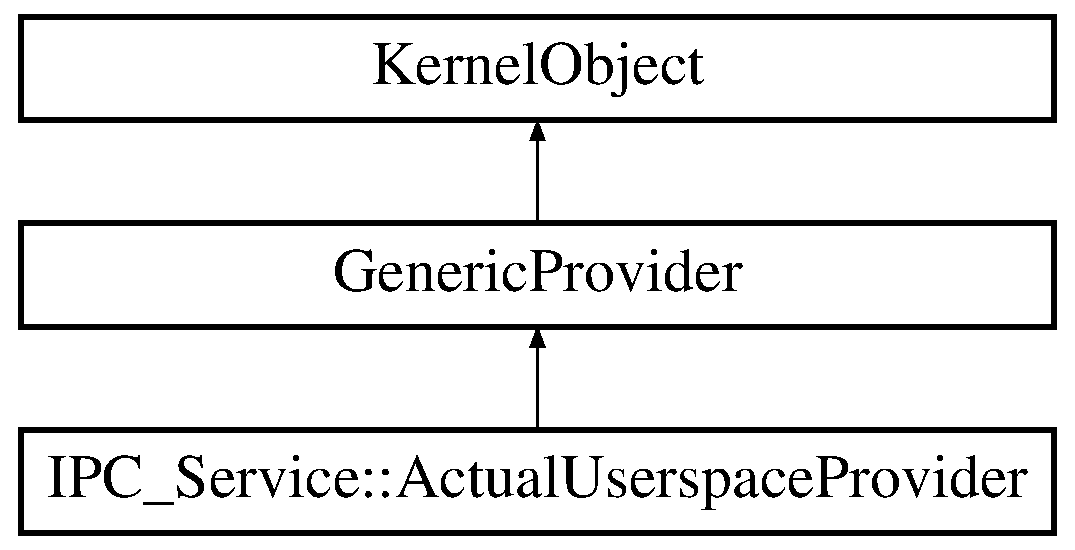
\includegraphics[height=3.000000cm]{class_i_p_c___service_1_1_actual_userspace_provider}
\end{center}
\end{figure}
\subsection*{Public Member Functions}
\begin{DoxyCompactItemize}
\item 
\mbox{\Hypertarget{class_i_p_c___service_1_1_actual_userspace_provider_ae0869d9c5fee31f786c69d239f9e212f}\label{class_i_p_c___service_1_1_actual_userspace_provider_ae0869d9c5fee31f786c69d239f9e212f}} 
const char $\ast$ {\bfseries Get\+Class\+Name} (U\+Int32 level)
\item 
\mbox{\Hypertarget{class_i_p_c___service_1_1_actual_userspace_provider_a5d89b927ecd4dedd01d02028588bc5cf}\label{class_i_p_c___service_1_1_actual_userspace_provider_a5d89b927ecd4dedd01d02028588bc5cf}} 
\hyperlink{class_i_p_c___service_1_1_userspace_provider}{Userspace\+Provider} $\ast$ {\bfseries Monitor} (void)
\item 
\mbox{\Hypertarget{class_i_p_c___service_1_1_actual_userspace_provider_ab41ede0b661c580bec3a653a404e9010}\label{class_i_p_c___service_1_1_actual_userspace_provider_ab41ede0b661c580bec3a653a404e9010}} 
\hyperlink{class_ipc_service}{Ipc\+Service} $\ast$ {\bfseries Launch\+Service} (\hyperlink{class_kernel_string}{Kernel\+String} $\ast$name, \hyperlink{class_kernel_string}{Kernel\+String} $\ast$type)
\item 
\mbox{\Hypertarget{class_i_p_c___service_1_1_actual_userspace_provider_a2a171142311c637e61e3b7615039f70f}\label{class_i_p_c___service_1_1_actual_userspace_provider_a2a171142311c637e61e3b7615039f70f}} 
bool {\bfseries Kill\+Service} (\hyperlink{class_ipc_service}{Ipc\+Service} $\ast$service)
\item 
\mbox{\Hypertarget{class_i_p_c___service_1_1_actual_userspace_provider_afcaa9880e30eda7b488e9225603da096}\label{class_i_p_c___service_1_1_actual_userspace_provider_afcaa9880e30eda7b488e9225603da096}} 
\hyperlink{class_ipc_client}{Ipc\+Client} $\ast$ {\bfseries Launch\+Client} (\hyperlink{class_kernel_string}{Kernel\+String} $\ast$name)
\item 
\mbox{\Hypertarget{class_i_p_c___service_1_1_actual_userspace_provider_a7ce03fcf818273560973087cfa541909}\label{class_i_p_c___service_1_1_actual_userspace_provider_a7ce03fcf818273560973087cfa541909}} 
bool {\bfseries Kill\+Client} (\hyperlink{class_ipc_client}{Ipc\+Client} $\ast$client)
\end{DoxyCompactItemize}
\subsection*{Protected Member Functions}
\begin{DoxyCompactItemize}
\item 
\mbox{\Hypertarget{class_i_p_c___service_1_1_actual_userspace_provider_ab29364220122b32e1b5ec64292a372ec}\label{class_i_p_c___service_1_1_actual_userspace_provider_ab29364220122b32e1b5ec64292a372ec}} 
\hyperlink{class_generic_provider_1_1_input_connection}{Input\+Connection} $\ast$ {\bfseries Input\+Connection\+Start} (\hyperlink{class_kernel_string}{Kernel\+String} $\ast$name, \hyperlink{class_ipc_endpoint}{Ipc\+Endpoint} $\ast$connection)
\item 
\mbox{\Hypertarget{class_i_p_c___service_1_1_actual_userspace_provider_ac07aeb354a483e9fa042be38fa827ff2}\label{class_i_p_c___service_1_1_actual_userspace_provider_ac07aeb354a483e9fa042be38fa827ff2}} 
void {\bfseries Input\+Connection\+Received} (\hyperlink{class_generic_provider_1_1_input_connection}{Input\+Connection} $\ast$connection, \hyperlink{class_kernel_buffer_memory}{Kernel\+Buffer\+Memory} $\ast$message)
\item 
\mbox{\Hypertarget{class_i_p_c___service_1_1_actual_userspace_provider_a5d5cc5a4d2c65398eb59400fb8ce149e}\label{class_i_p_c___service_1_1_actual_userspace_provider_a5d5cc5a4d2c65398eb59400fb8ce149e}} 
void {\bfseries Input\+Connection\+End} (\hyperlink{class_generic_provider_1_1_input_connection}{Input\+Connection} $\ast$connection)
\item 
\mbox{\Hypertarget{class_i_p_c___service_1_1_actual_userspace_provider_ad5a2568fa7eb45f94ddba0b889386d3a}\label{class_i_p_c___service_1_1_actual_userspace_provider_ad5a2568fa7eb45f94ddba0b889386d3a}} 
\hyperlink{class_generic_provider_1_1_output_connection}{Output\+Connection} $\ast$ {\bfseries Output\+Connection\+Start} (\hyperlink{class_generic_provider_1_1_service}{Service} $\ast$source, \hyperlink{class_ipc_endpoint}{Ipc\+Endpoint} $\ast$connection)
\item 
\mbox{\Hypertarget{class_i_p_c___service_1_1_actual_userspace_provider_a74ed15be91e351e5fd43638bd924cb9c}\label{class_i_p_c___service_1_1_actual_userspace_provider_a74ed15be91e351e5fd43638bd924cb9c}} 
void {\bfseries Output\+Connection\+Message} (\hyperlink{class_generic_provider_1_1_output_connection}{Output\+Connection} $\ast$connection, \hyperlink{class_kernel_buffer_memory}{Kernel\+Buffer\+Memory} $\ast$message)
\item 
\mbox{\Hypertarget{class_i_p_c___service_1_1_actual_userspace_provider_a590138d1fa024ef456c44e667057ac69}\label{class_i_p_c___service_1_1_actual_userspace_provider_a590138d1fa024ef456c44e667057ac69}} 
void {\bfseries Output\+Connection\+End} (\hyperlink{class_generic_provider_1_1_output_connection}{Output\+Connection} $\ast$old\+Connection)
\end{DoxyCompactItemize}
\subsection*{Private Attributes}
\begin{DoxyCompactItemize}
\item 
\mbox{\Hypertarget{class_i_p_c___service_1_1_actual_userspace_provider_a7f4aeb528e64d2d2fe8fdbb2c37f2955}\label{class_i_p_c___service_1_1_actual_userspace_provider_a7f4aeb528e64d2d2fe8fdbb2c37f2955}} 
\hyperlink{class_kernel_array}{Kernel\+Array} $\ast$ {\bfseries \+\_\+client\+List}
\item 
\mbox{\Hypertarget{class_i_p_c___service_1_1_actual_userspace_provider_abb248dc9a45587ca57312567c0a64d9f}\label{class_i_p_c___service_1_1_actual_userspace_provider_abb248dc9a45587ca57312567c0a64d9f}} 
\hyperlink{class_kernel_dictionary}{Kernel\+Dictionary} $\ast$ {\bfseries \+\_\+service\+Map}
\item 
\mbox{\Hypertarget{class_i_p_c___service_1_1_actual_userspace_provider_a93bed89a71e39e57af21b58652bd7343}\label{class_i_p_c___service_1_1_actual_userspace_provider_a93bed89a71e39e57af21b58652bd7343}} 
\hyperlink{class_i_p_c___service_1_1_userspace_provider}{Userspace\+Provider} $\ast$ {\bfseries \+\_\+monitor}
\end{DoxyCompactItemize}
\subsection*{Additional Inherited Members}


The documentation for this class was generated from the following file\+:\begin{DoxyCompactItemize}
\item 
I\+P\+C\+\_\+\+Service.\+cpp\end{DoxyCompactItemize}

\hypertarget{class_internal_1_1_allocation}{}\section{Internal\+:\+:Allocation Class Reference}
\label{class_internal_1_1_allocation}\index{Internal\+::\+Allocation@{Internal\+::\+Allocation}}
Inheritance diagram for Internal\+:\+:Allocation\+:\begin{figure}[H]
\begin{center}
\leavevmode
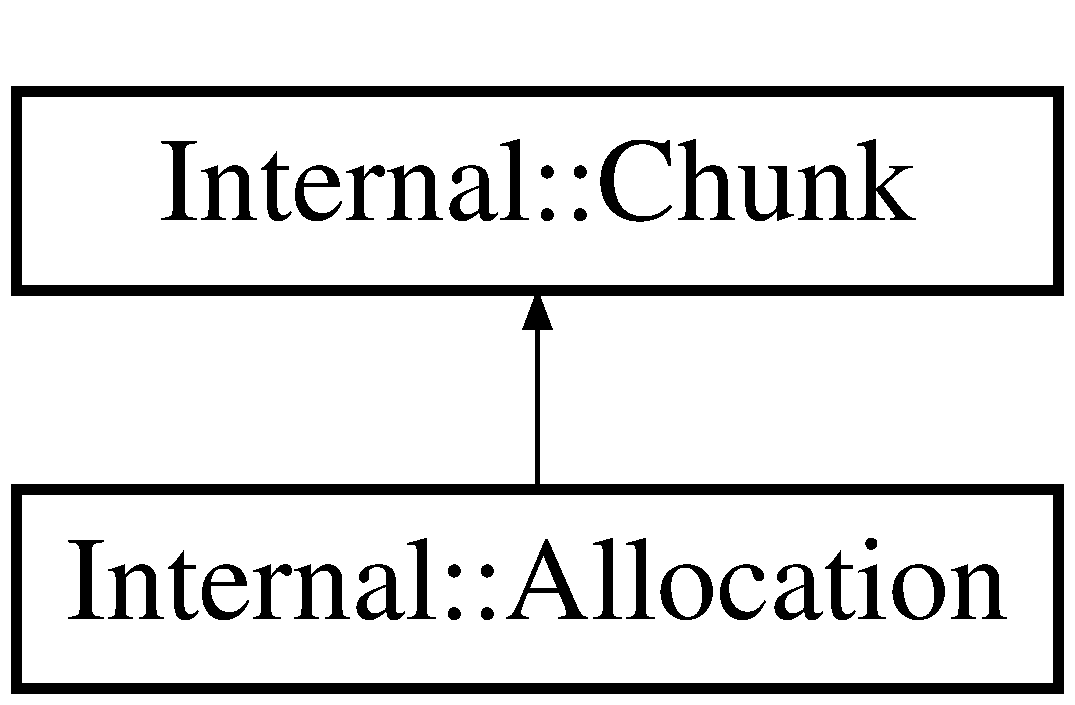
\includegraphics[height=2.000000cm]{class_internal_1_1_allocation}
\end{center}
\end{figure}
\subsection*{Public Member Functions}
\begin{DoxyCompactItemize}
\item 
\mbox{\Hypertarget{class_internal_1_1_allocation_ad816879b0a1f16cbbfda811ba35c83e6}\label{class_internal_1_1_allocation_ad816879b0a1f16cbbfda811ba35c83e6}} 
{\bfseries Allocation} (Basic\+Heap\+::h\+\_\+size size)
\item 
\mbox{\Hypertarget{class_internal_1_1_allocation_aafab9a6049ad889fc98c6e9e508e7ef3}\label{class_internal_1_1_allocation_aafab9a6049ad889fc98c6e9e508e7ef3}} 
void $\ast$ {\bfseries Get\+Pointer} (void)
\end{DoxyCompactItemize}
\subsection*{Static Public Member Functions}
\begin{DoxyCompactItemize}
\item 
\mbox{\Hypertarget{class_internal_1_1_allocation_a66e5cabfad8f06c9ce7a8cb17e40ed02}\label{class_internal_1_1_allocation_a66e5cabfad8f06c9ce7a8cb17e40ed02}} 
static \hyperlink{class_internal_1_1_allocation}{Allocation} $\ast$ {\bfseries Get\+Object} (void $\ast$pointer)
\end{DoxyCompactItemize}
\subsection*{Private Member Functions}
\begin{DoxyCompactItemize}
\item 
\mbox{\Hypertarget{class_internal_1_1_allocation_a6316094a356a6a483a1988a15199867c}\label{class_internal_1_1_allocation_a6316094a356a6a483a1988a15199867c}} 
void {\bfseries Scrub} (void)
\end{DoxyCompactItemize}
\subsection*{Additional Inherited Members}


The documentation for this class was generated from the following file\+:\begin{DoxyCompactItemize}
\item 
Basic\+Heap.\+cpp\end{DoxyCompactItemize}

\hypertarget{class_a_t_a_driver}{}\section{A\+T\+A\+Driver Class Reference}
\label{class_a_t_a_driver}\index{A\+T\+A\+Driver@{A\+T\+A\+Driver}}
Inheritance diagram for A\+T\+A\+Driver\+:\begin{figure}[H]
\begin{center}
\leavevmode
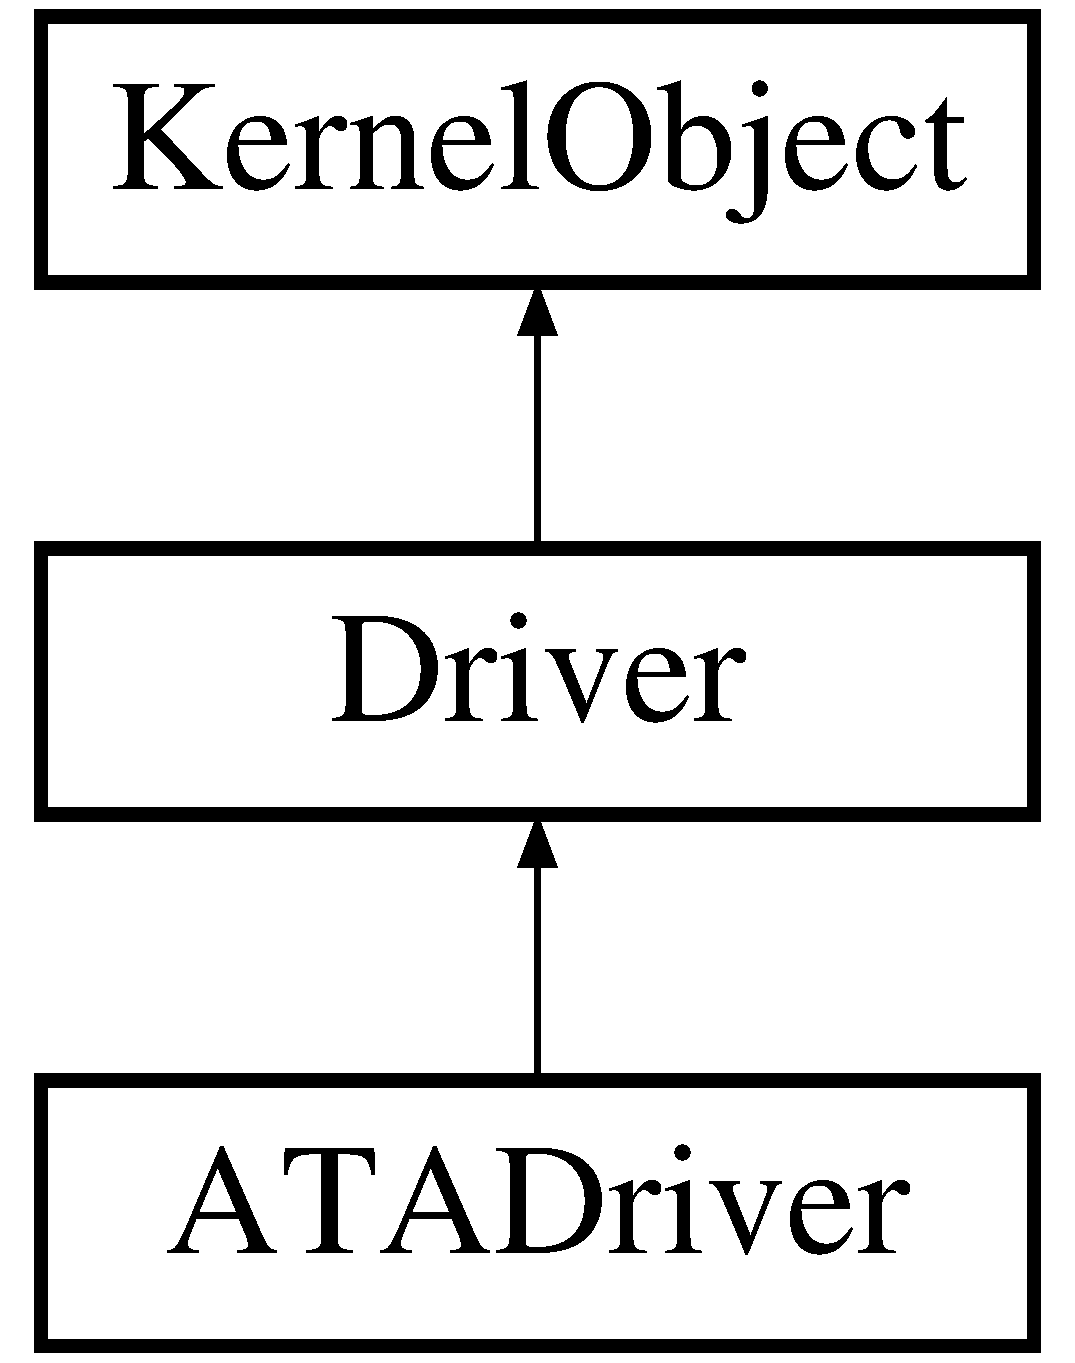
\includegraphics[height=3.000000cm]{class_a_t_a_driver}
\end{center}
\end{figure}
\subsection*{Classes}
\begin{DoxyCompactItemize}
\item 
struct \hyperlink{struct_a_t_a_driver_1_1_r_e_g___c_m_d___i_n_f_o}{R\+E\+G\+\_\+\+C\+M\+D\+\_\+\+I\+N\+FO}
\item 
union \hyperlink{union_a_t_a_driver_1_1_s_t_a_t___r_e_g}{S\+T\+A\+T\+\_\+\+R\+EG}
\end{DoxyCompactItemize}
\subsection*{Public Types}
\begin{DoxyCompactItemize}
\item 
\mbox{\Hypertarget{class_a_t_a_driver_a4850f4b56a51bb6a52c23db2408ff672}\label{class_a_t_a_driver_a4850f4b56a51bb6a52c23db2408ff672}} 
enum {\bfseries C\+O\+M\+M\+A\+ND} \{ \newline
{\bfseries cmd\+C\+F\+A\+\_\+\+E\+R\+A\+S\+E\+\_\+\+S\+E\+C\+T\+O\+RS} = 0x\+C0, 
{\bfseries cmd\+C\+F\+A\+\_\+\+R\+E\+Q\+U\+E\+S\+T\+\_\+\+E\+X\+T\+\_\+\+E\+R\+R\+\_\+\+C\+O\+DE} = 0x03, 
{\bfseries cmd\+C\+F\+A\+\_\+\+T\+R\+A\+N\+S\+L\+A\+T\+E\+\_\+\+S\+E\+C\+T\+OR} = 0x87, 
{\bfseries cmd\+C\+F\+A\+\_\+\+W\+R\+I\+T\+E\+\_\+\+M\+U\+L\+T\+I\+P\+L\+E\+\_\+\+W\+O\+\_\+\+E\+R\+A\+SE} = 0x\+CD, 
\newline
{\bfseries cmd\+C\+F\+A\+\_\+\+W\+R\+I\+T\+E\+\_\+\+S\+E\+C\+T\+O\+R\+S\+\_\+\+W\+O\+\_\+\+E\+R\+A\+SE} = 0x38, 
{\bfseries cmd\+C\+H\+E\+C\+K\+\_\+\+P\+O\+W\+E\+R\+\_\+\+M\+O\+D\+E1} = 0x\+E5, 
{\bfseries cmd\+C\+H\+E\+C\+K\+\_\+\+P\+O\+W\+E\+R\+\_\+\+M\+O\+D\+E2} = 0x98, 
{\bfseries cmd\+D\+E\+V\+I\+C\+E\+\_\+\+R\+E\+S\+ET} = 0x08, 
\newline
{\bfseries cmd\+E\+X\+E\+C\+U\+T\+E\+\_\+\+D\+E\+V\+I\+C\+E\+\_\+\+D\+I\+A\+G\+N\+O\+S\+T\+IC} = 0x90, 
{\bfseries cmd\+F\+L\+U\+S\+H\+\_\+\+C\+A\+C\+HE} = 0x\+E7, 
{\bfseries cmd\+F\+L\+U\+S\+H\+\_\+\+C\+A\+C\+H\+E\+\_\+\+E\+XT} = 0x\+EA, 
{\bfseries cmd\+F\+O\+R\+M\+A\+T\+\_\+\+T\+R\+A\+CK} = 0x50, 
\newline
{\bfseries cmd\+I\+D\+E\+N\+T\+I\+F\+Y\+\_\+\+D\+E\+V\+I\+CE} = 0x\+EC, 
{\bfseries cmd\+I\+D\+E\+N\+T\+I\+F\+Y\+\_\+\+D\+E\+V\+I\+C\+E\+\_\+\+P\+A\+C\+K\+ET} = 0x\+A1, 
{\bfseries cmd\+I\+D\+E\+N\+T\+I\+F\+Y\+\_\+\+P\+A\+C\+K\+E\+T\+\_\+\+D\+E\+V\+I\+CE} = 0x\+A1, 
{\bfseries cmd\+I\+D\+L\+E1} = 0x\+E3, 
\newline
{\bfseries cmd\+I\+D\+L\+E2} = 0x97, 
{\bfseries cmd\+I\+D\+L\+E\+\_\+\+I\+M\+M\+E\+D\+I\+A\+T\+E1} = 0x\+E1, 
{\bfseries cmd\+I\+D\+L\+E\+\_\+\+I\+M\+M\+E\+D\+I\+A\+T\+E2} = 0x95, 
{\bfseries cmd\+I\+N\+I\+T\+I\+A\+L\+I\+Z\+E\+\_\+\+D\+R\+I\+V\+E\+\_\+\+P\+A\+R\+A\+M\+E\+T\+E\+RS} = 0x91, 
\newline
{\bfseries cmd\+I\+N\+I\+T\+I\+A\+L\+I\+Z\+E\+\_\+\+D\+E\+V\+I\+C\+E\+\_\+\+P\+A\+R\+A\+M\+E\+T\+E\+RS} = 0x91, 
{\bfseries cmd\+N\+OP} = 0x00, 
{\bfseries cmd\+P\+A\+C\+K\+ET} = 0x\+A0, 
{\bfseries cmd\+R\+E\+A\+D\+\_\+\+B\+U\+F\+F\+ER} = 0x\+E4, 
\newline
{\bfseries cmd\+R\+E\+A\+D\+\_\+\+D\+MA} = 0x\+C8, 
{\bfseries cmd\+R\+E\+A\+D\+\_\+\+D\+M\+A\+\_\+\+E\+XT} = 0x25, 
{\bfseries cmd\+R\+E\+A\+D\+\_\+\+D\+M\+A\+\_\+\+Q\+U\+E\+U\+ED} = 0x\+C7, 
{\bfseries cmd\+R\+E\+A\+D\+\_\+\+D\+M\+A\+\_\+\+Q\+U\+E\+U\+E\+D\+\_\+\+E\+XT} = 0x26, 
\newline
{\bfseries cmd\+R\+E\+A\+D\+\_\+\+M\+U\+L\+T\+I\+P\+LE} = 0x\+C4, 
{\bfseries cmd\+R\+E\+A\+D\+\_\+\+M\+U\+L\+T\+I\+P\+L\+E\+\_\+\+E\+XT} = 0x29, 
{\bfseries cmd\+R\+E\+A\+D\+\_\+\+S\+E\+C\+T\+O\+RS} = 0x20, 
{\bfseries cmd\+R\+E\+A\+D\+\_\+\+S\+E\+C\+T\+O\+R\+S\+\_\+\+E\+XT} = 0x24, 
\newline
{\bfseries cmd\+R\+E\+A\+D\+\_\+\+V\+E\+R\+I\+F\+Y\+\_\+\+S\+E\+C\+T\+O\+RS} = 0x40, 
{\bfseries cmd\+R\+E\+A\+D\+\_\+\+V\+E\+R\+I\+F\+Y\+\_\+\+S\+E\+C\+T\+O\+R\+S\+\_\+\+E\+XT} = 0x42, 
{\bfseries cmd\+R\+E\+C\+A\+L\+I\+B\+R\+A\+TE} = 0x10, 
{\bfseries cmd\+S\+E\+EK} = 0x70, 
\newline
{\bfseries cmd\+S\+E\+T\+\_\+\+F\+E\+A\+T\+U\+R\+ES} = 0x\+EF, 
{\bfseries cmd\+S\+E\+T\+\_\+\+M\+U\+L\+T\+I\+P\+L\+E\+\_\+\+M\+O\+DE} = 0x\+C6, 
{\bfseries cmd\+S\+L\+E\+E\+P1} = 0x\+E6, 
{\bfseries cmd\+S\+L\+E\+E\+P2} = 0x99, 
\newline
{\bfseries cmd\+S\+M\+A\+RT} = 0x\+B0, 
{\bfseries cmd\+S\+T\+A\+N\+D\+B\+Y1} = 0x\+E2, 
{\bfseries cmd\+S\+T\+A\+N\+D\+B\+Y2} = 0x96, 
{\bfseries cmd\+S\+T\+A\+N\+D\+B\+Y\+\_\+\+I\+M\+M\+E\+D\+I\+A\+T\+E1} = 0x\+E0, 
\newline
{\bfseries cmd\+S\+T\+A\+N\+D\+B\+Y\+\_\+\+I\+M\+M\+E\+D\+I\+A\+T\+E2} = 0x94, 
{\bfseries cmd\+W\+R\+I\+T\+E\+\_\+\+B\+U\+F\+F\+ER} = 0x\+E8, 
{\bfseries cmd\+W\+R\+I\+T\+E\+\_\+\+D\+MA} = 0x\+CA, 
{\bfseries cmd\+W\+R\+I\+T\+E\+\_\+\+D\+M\+A\+\_\+\+E\+XT} = 0x35, 
\newline
{\bfseries cmd\+W\+R\+I\+T\+E\+\_\+\+D\+M\+A\+\_\+\+Q\+U\+E\+U\+ED} = 0x\+CC, 
{\bfseries cmd\+W\+R\+I\+T\+E\+\_\+\+D\+M\+A\+\_\+\+Q\+U\+E\+U\+E\+D\+\_\+\+E\+XT} = 0x36, 
{\bfseries cmd\+W\+R\+I\+T\+E\+\_\+\+M\+U\+L\+T\+I\+P\+LE} = 0x\+C5, 
{\bfseries cmd\+W\+R\+I\+T\+E\+\_\+\+M\+U\+L\+T\+I\+P\+L\+E\+\_\+\+E\+XT} = 0x39, 
\newline
{\bfseries cmd\+W\+R\+I\+T\+E\+\_\+\+S\+E\+C\+T\+O\+RS} = 0x30, 
{\bfseries cmd\+W\+R\+I\+T\+E\+\_\+\+S\+E\+C\+T\+O\+R\+S\+\_\+\+E\+XT} = 0x34, 
{\bfseries cmd\+W\+R\+I\+T\+E\+\_\+\+V\+E\+R\+I\+FY} = 0x3C
 \}
\item 
\mbox{\Hypertarget{class_a_t_a_driver_a2abcb2093e0beb44ed5b5f71611e57aa}\label{class_a_t_a_driver_a2abcb2093e0beb44ed5b5f71611e57aa}} 
enum {\bfseries L\+B\+A\+\_\+\+S\+I\+ZE} \{ {\bfseries lba\+C\+HS} = 0, 
{\bfseries lba28} = 28, 
{\bfseries lba48} = 48
 \}
\item 
\mbox{\Hypertarget{class_a_t_a_driver_a48384380799c33052841dcbb45e0e155}\label{class_a_t_a_driver_a48384380799c33052841dcbb45e0e155}} 
enum {\bfseries D\+E\+V\+\_\+\+C\+O\+N\+F\+IG} \{ \newline
{\bfseries dc\+None} = 0, 
{\bfseries dc\+Unknown} = 1, 
{\bfseries dc\+P\+A\+TA} = 2, 
{\bfseries dc\+P\+A\+T\+A\+PI} = 4, 
\newline
{\bfseries dc\+S\+A\+TA} = 2 + 8, 
{\bfseries dc\+S\+A\+T\+A\+PI} = 4 + 8
 \}
\end{DoxyCompactItemize}
\subsection*{Public Member Functions}
\begin{DoxyCompactItemize}
\item 
\mbox{\Hypertarget{class_a_t_a_driver_a8d56d9f4b87682c25e695014a6c22f28}\label{class_a_t_a_driver_a8d56d9f4b87682c25e695014a6c22f28}} 
const char $\ast$ {\bfseries Get\+Class\+Name} (U\+Int32 level)
\item 
\mbox{\Hypertarget{class_a_t_a_driver_a513bb44e2306fd92d7f235efd2450d28}\label{class_a_t_a_driver_a513bb44e2306fd92d7f235efd2450d28}} 
bool {\bfseries Start} (\hyperlink{class_driver}{Driver} $\ast$parent)
\item 
\mbox{\Hypertarget{class_a_t_a_driver_a60a7add2dcd7b21d8c927b6a32bc9ade}\label{class_a_t_a_driver_a60a7add2dcd7b21d8c927b6a32bc9ade}} 
void {\bfseries Stop} (void)
\end{DoxyCompactItemize}
\subsection*{Static Public Member Functions}
\begin{DoxyCompactItemize}
\item 
\mbox{\Hypertarget{class_a_t_a_driver_aa0d70f348001d302c2636679dbf384f2}\label{class_a_t_a_driver_aa0d70f348001d302c2636679dbf384f2}} 
static void {\bfseries Install} (void)
\end{DoxyCompactItemize}
\subsection*{Private Member Functions}
\begin{DoxyCompactItemize}
\item 
\mbox{\Hypertarget{class_a_t_a_driver_ad3d6512578f1cbb9227bde5e9ecbc7e7}\label{class_a_t_a_driver_ad3d6512578f1cbb9227bde5e9ecbc7e7}} 
\hyperlink{class_a_t_a_driver_node}{A\+T\+A\+Driver\+Node} $\ast$ {\bfseries I\+O\+Port} (void)
\item 
\mbox{\Hypertarget{class_a_t_a_driver_a59a29742ad53b92cc30109ec06b4e994}\label{class_a_t_a_driver_a59a29742ad53b92cc30109ec06b4e994}} 
void {\bfseries Start\+Timer} (void)
\item 
\mbox{\Hypertarget{class_a_t_a_driver_a49229a68f9dc58114d54246bdc0a7ae5}\label{class_a_t_a_driver_a49229a68f9dc58114d54246bdc0a7ae5}} 
int {\bfseries Configure} (void)
\item 
\mbox{\Hypertarget{class_a_t_a_driver_adb2eadde039bbfc3f1e8dba326ce61c2}\label{class_a_t_a_driver_adb2eadde039bbfc3f1e8dba326ce61c2}} 
bool {\bfseries Reset} (U\+Int32 device\+Return)
\item 
\mbox{\Hypertarget{class_a_t_a_driver_a877c90a14c27f0bd4c2fbbd29236e5af}\label{class_a_t_a_driver_a877c90a14c27f0bd4c2fbbd29236e5af}} 
bool {\bfseries Non\+Data\+Command\+L\+B\+A28} (U\+Int8 dev, C\+O\+M\+M\+A\+ND command, U\+Int32 sector, U\+Int32 lba)
\item 
\mbox{\Hypertarget{class_a_t_a_driver_a8cb0839e7e217848aa085c151cbbdb48}\label{class_a_t_a_driver_a8cb0839e7e217848aa085c151cbbdb48}} 
bool {\bfseries Non\+Data\+Command\+L\+B\+A48} (U\+Int8 dev, C\+O\+M\+M\+A\+ND command, U\+Int32 sector, U\+Int64 lba)
\item 
\mbox{\Hypertarget{class_a_t_a_driver_a4c141442bc319326e9a5b0439e4b75af}\label{class_a_t_a_driver_a4c141442bc319326e9a5b0439e4b75af}} 
bool {\bfseries Data\+Command\+L\+B\+A28\+In} (U\+Int8 device, C\+O\+M\+M\+A\+ND command, U\+Int32 lba, void $\ast$buffer, U\+Int32 num\+Sectors, U\+Int32 multi\+Cnt)
\item 
\mbox{\Hypertarget{class_a_t_a_driver_a72ed03e250b408a87449e98062ca8743}\label{class_a_t_a_driver_a72ed03e250b408a87449e98062ca8743}} 
bool {\bfseries Data\+Command\+L\+B\+A48\+In} (U\+Int8 device, C\+O\+M\+M\+A\+ND command, U\+Int64 lba, void $\ast$buffer, U\+Int32 num\+Sectors, U\+Int32 multi\+Cnt)
\item 
\mbox{\Hypertarget{class_a_t_a_driver_aa9b2e4ca088d4a8fcd91225d49bef47e}\label{class_a_t_a_driver_aa9b2e4ca088d4a8fcd91225d49bef47e}} 
bool {\bfseries Data\+Command\+L\+B\+A28\+Out} (U\+Int8 device, C\+O\+M\+M\+A\+ND command, U\+Int32 lba, void $\ast$buffer, U\+Int32 num\+Sectors, U\+Int32 multi\+Cnt)
\item 
\mbox{\Hypertarget{class_a_t_a_driver_a4ce19d0707488daebbc1c920359580dd}\label{class_a_t_a_driver_a4ce19d0707488daebbc1c920359580dd}} 
bool {\bfseries Data\+Command\+L\+B\+A48\+Out} (U\+Int8 device, C\+O\+M\+M\+A\+ND command, U\+Int64 lba, void $\ast$buffer, U\+Int32 num\+Sectors, U\+Int32 multi\+Cnt)
\item 
\mbox{\Hypertarget{class_a_t_a_driver_a62fe17dec81c828ef93ff588801b0624}\label{class_a_t_a_driver_a62fe17dec81c828ef93ff588801b0624}} 
bool {\bfseries Packet} (U\+Int8 device, char $\ast$control\+Buffer, U\+Int32 control\+Buffer\+Length, bool direction\+Out, void $\ast$data\+Buffer, U\+Int32 data\+Buffer\+Length)
\item 
\mbox{\Hypertarget{class_a_t_a_driver_a3170301817f7d44bc202e4e326aaec00}\label{class_a_t_a_driver_a3170301817f7d44bc202e4e326aaec00}} 
bool {\bfseries \+\_\+\+Exec\+Non\+Data\+Command} (U\+Int32 device)
\item 
\mbox{\Hypertarget{class_a_t_a_driver_a1b0854d1ed7a43e16cb9d0c3274652de}\label{class_a_t_a_driver_a1b0854d1ed7a43e16cb9d0c3274652de}} 
bool {\bfseries \+\_\+\+Exec\+Data\+Command\+In} (U\+Int32 device, U\+Int8 $\ast$buffer, U\+Int32 num\+Sectors, U\+Int32 multi\+Cnt)
\item 
\mbox{\Hypertarget{class_a_t_a_driver_a4ce795695fe10ccd25ef837b75574c5a}\label{class_a_t_a_driver_a4ce795695fe10ccd25ef837b75574c5a}} 
bool {\bfseries \+\_\+\+Exec\+Data\+Command\+Out} (U\+Int32 device, U\+Int8 $\ast$buffer, U\+Int32 num\+Sectors, U\+Int32 multi\+Cnt)
\item 
\mbox{\Hypertarget{class_a_t_a_driver_ab4e1ce0fdce3f184d016cb79c31a5770}\label{class_a_t_a_driver_ab4e1ce0fdce3f184d016cb79c31a5770}} 
bool {\bfseries \+\_\+\+Configure\+\_\+\+Init\+Device} (U\+Int8 device)
\item 
\mbox{\Hypertarget{class_a_t_a_driver_adc6ea8fed5cbf4fca899dde0e9fadf32}\label{class_a_t_a_driver_adc6ea8fed5cbf4fca899dde0e9fadf32}} 
D\+E\+V\+\_\+\+C\+O\+N\+F\+IG {\bfseries \+\_\+\+Configure\+\_\+\+Check\+Device} (U\+Int8 device)
\item 
\mbox{\Hypertarget{class_a_t_a_driver_a7d2626a7abf37076b39e1042571d7075}\label{class_a_t_a_driver_a7d2626a7abf37076b39e1042571d7075}} 
bool {\bfseries \+\_\+\+Select} (U\+Int8 device)
\item 
\mbox{\Hypertarget{class_a_t_a_driver_a97fd5077fcc89d5abef66326170f47a1}\label{class_a_t_a_driver_a97fd5077fcc89d5abef66326170f47a1}} 
void {\bfseries \+\_\+\+Setup\+Command} (void)
\item 
\mbox{\Hypertarget{class_a_t_a_driver_af1abb7ccb25080d5d5800f8ab8d9eefb}\label{class_a_t_a_driver_af1abb7ccb25080d5d5800f8ab8d9eefb}} 
void {\bfseries \+\_\+\+Wait} (U\+Int8 we, U\+Int8 pe)
\item 
\mbox{\Hypertarget{class_a_t_a_driver_aaf8eaa3f5495338155371dfd7d602bca}\label{class_a_t_a_driver_aaf8eaa3f5495338155371dfd7d602bca}} 
bool {\bfseries \+\_\+\+Complete\+Command} (void)
\item 
\mbox{\Hypertarget{class_a_t_a_driver_a10ce5d2f8ea48bbc45d7cee8dac57312}\label{class_a_t_a_driver_a10ce5d2f8ea48bbc45d7cee8dac57312}} 
void {\bfseries \+\_\+drq\+Block\+Out} (U\+Int8 address\+Data\+Register, U\+Int8 $\ast$buffer, U\+Int32 word\+Count)
\item 
\mbox{\Hypertarget{class_a_t_a_driver_a2dd7b6d944cd27bcf5826db3c38d1fae}\label{class_a_t_a_driver_a2dd7b6d944cd27bcf5826db3c38d1fae}} 
void {\bfseries \+\_\+drq\+Block\+In} (U\+Int8 address\+Data\+Register, U\+Int8 $\ast$buffer, U\+Int32 word\+Count)
\end{DoxyCompactItemize}
\subsection*{Private Attributes}
\begin{DoxyCompactItemize}
\item 
\mbox{\Hypertarget{class_a_t_a_driver_a299e08933068e464e7ee562e67951125}\label{class_a_t_a_driver_a299e08933068e464e7ee562e67951125}} 
friend {\bfseries Configure\+A\+TA}
\item 
\mbox{\Hypertarget{class_a_t_a_driver_af032ff6894fb0c425c2c22f7a5c688f9}\label{class_a_t_a_driver_af032ff6894fb0c425c2c22f7a5c688f9}} 
bool {\bfseries \+\_\+use\+Interrupts}
\item 
\mbox{\Hypertarget{class_a_t_a_driver_a691e4861fbc5c4fc3e443c1edbbc5c63}\label{class_a_t_a_driver_a691e4861fbc5c4fc3e443c1edbbc5c63}} 
\hyperlink{class_d_m_a_buffer}{D\+M\+A\+Buffer} $\ast$ {\bfseries \+\_\+dma\+Buffer}
\item 
\mbox{\Hypertarget{class_a_t_a_driver_aa7adcb4899b49a62b044d1ccd8e8bffd}\label{class_a_t_a_driver_aa7adcb4899b49a62b044d1ccd8e8bffd}} 
\hyperlink{class_timer}{Timer} $\ast$ {\bfseries \+\_\+timer}
\item 
\mbox{\Hypertarget{class_a_t_a_driver_a9eeaebd9d84acf04f8c0c7dfe48469ba}\label{class_a_t_a_driver_a9eeaebd9d84acf04f8c0c7dfe48469ba}} 
\hyperlink{class_signal_or}{Signal\+Or} $\ast$ {\bfseries \+\_\+wait\+Object}
\item 
\mbox{\Hypertarget{class_a_t_a_driver_a951c3b398478fe0bb091ec2d59a95c72}\label{class_a_t_a_driver_a951c3b398478fe0bb091ec2d59a95c72}} 
\hyperlink{class_ipc_service_proxy}{Ipc\+Service\+Proxy} $\ast$ {\bfseries \+\_\+service\+List}
\item 
\mbox{\Hypertarget{class_a_t_a_driver_ad5bb2f1f2ed0bbd54bc7c3a4fe493fce}\label{class_a_t_a_driver_ad5bb2f1f2ed0bbd54bc7c3a4fe493fce}} 
\hyperlink{class_dispatch_queue}{Dispatch\+Queue} $\ast$ {\bfseries \+\_\+main\+Queue}
\item 
\mbox{\Hypertarget{class_a_t_a_driver_ab4f21c70537fa68080e8a80680b7bd11}\label{class_a_t_a_driver_ab4f21c70537fa68080e8a80680b7bd11}} 
\hyperlink{class_a_t_a_driver_drive}{A\+T\+A\+Driver\+Drive} $\ast$ {\bfseries \+\_\+drive\+Handlers} \mbox{[}2\mbox{]}
\item 
\mbox{\Hypertarget{class_a_t_a_driver_ab6564764135aee3cc8ca3e833361e7b8}\label{class_a_t_a_driver_ab6564764135aee3cc8ca3e833361e7b8}} 
U\+Int8 {\bfseries \+\_\+pio\+Transfer\+Width}
\item 
\mbox{\Hypertarget{class_a_t_a_driver_a3c6c789a1d434d6778b1b8a59c28c524}\label{class_a_t_a_driver_a3c6c789a1d434d6778b1b8a59c28c524}} 
\hyperlink{struct_a_t_a_driver_1_1_r_e_g___c_m_d___i_n_f_o}{R\+E\+G\+\_\+\+C\+M\+D\+\_\+\+I\+N\+FO} {\bfseries \+\_\+reg\+Command\+Info}
\item 
\mbox{\Hypertarget{class_a_t_a_driver_a72cef04690e6c5f88880674b7a446330}\label{class_a_t_a_driver_a72cef04690e6c5f88880674b7a446330}} 
D\+E\+V\+\_\+\+C\+O\+N\+F\+IG {\bfseries \+\_\+config\+Info} \mbox{[}2\mbox{]}
\item 
\mbox{\Hypertarget{class_a_t_a_driver_a4167e083539c514f9c918eaaa53498d9}\label{class_a_t_a_driver_a4167e083539c514f9c918eaaa53498d9}} 
friend {\bfseries A\+T\+A\+Driver\+Drive\+\_\+\+A\+T\+A\+PI}
\item 
\mbox{\Hypertarget{class_a_t_a_driver_af445e273bc5912b83369c581ba906e1b}\label{class_a_t_a_driver_af445e273bc5912b83369c581ba906e1b}} 
friend {\bfseries A\+T\+A\+Driver\+Drive\+\_\+\+A\+TA}
\end{DoxyCompactItemize}
\subsection*{Additional Inherited Members}


The documentation for this class was generated from the following files\+:\begin{DoxyCompactItemize}
\item 
Driver\+\_\+\+A\+T\+A.\+h\item 
Driver\+\_\+\+A\+T\+A.\+cpp\end{DoxyCompactItemize}

\hypertarget{class_a_t_a_driver___factory}{}\section{A\+T\+A\+Driver\+\_\+\+Factory Class Reference}
\label{class_a_t_a_driver___factory}\index{A\+T\+A\+Driver\+\_\+\+Factory@{A\+T\+A\+Driver\+\_\+\+Factory}}
Inheritance diagram for A\+T\+A\+Driver\+\_\+\+Factory\+:\begin{figure}[H]
\begin{center}
\leavevmode
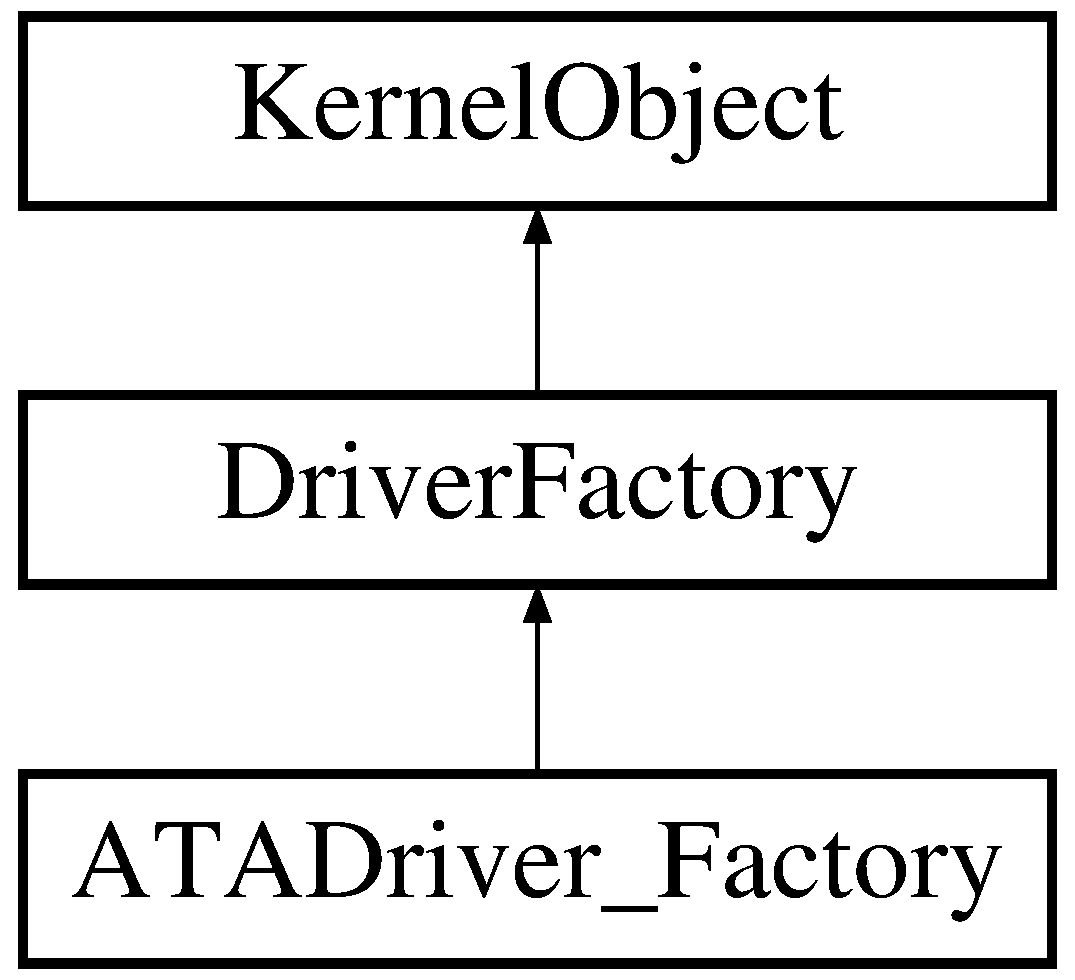
\includegraphics[height=3.000000cm]{class_a_t_a_driver___factory}
\end{center}
\end{figure}
\subsection*{Classes}
\begin{DoxyCompactItemize}
\item 
class \hyperlink{class_a_t_a_driver___factory_1_1_a_t_a_driver___match}{A\+T\+A\+Driver\+\_\+\+Match}
\end{DoxyCompactItemize}
\subsection*{Public Member Functions}
\begin{DoxyCompactItemize}
\item 
\mbox{\Hypertarget{class_a_t_a_driver___factory_ab6565ae7815e3c67d22f04b3a35edc5c}\label{class_a_t_a_driver___factory_ab6565ae7815e3c67d22f04b3a35edc5c}} 
const char $\ast$ {\bfseries Get\+Class\+Name} (U\+Int32 level)
\item 
\mbox{\Hypertarget{class_a_t_a_driver___factory_a1387aaec1518a594f1eaa3530518444a}\label{class_a_t_a_driver___factory_a1387aaec1518a594f1eaa3530518444a}} 
\hyperlink{class_kernel_array}{Kernel\+Array} $\ast$ {\bfseries Match\+For\+Parent} (\hyperlink{class_driver}{Driver} $\ast$parent)
\end{DoxyCompactItemize}
\subsection*{Additional Inherited Members}


The documentation for this class was generated from the following file\+:\begin{DoxyCompactItemize}
\item 
Driver\+\_\+\+A\+T\+A.\+cpp\end{DoxyCompactItemize}

\hypertarget{class_a_t_a_driver___factory_1_1_a_t_a_driver___match}{}\section{A\+T\+A\+Driver\+\_\+\+Factory\+:\+:A\+T\+A\+Driver\+\_\+\+Match Class Reference}
\label{class_a_t_a_driver___factory_1_1_a_t_a_driver___match}\index{A\+T\+A\+Driver\+\_\+\+Factory\+::\+A\+T\+A\+Driver\+\_\+\+Match@{A\+T\+A\+Driver\+\_\+\+Factory\+::\+A\+T\+A\+Driver\+\_\+\+Match}}
Inheritance diagram for A\+T\+A\+Driver\+\_\+\+Factory\+:\+:A\+T\+A\+Driver\+\_\+\+Match\+:\begin{figure}[H]
\begin{center}
\leavevmode
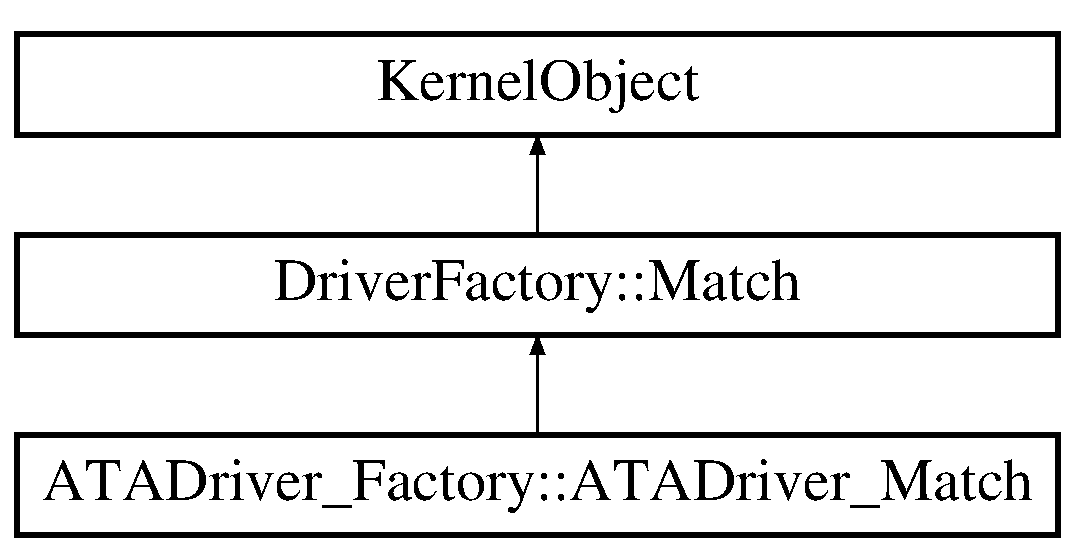
\includegraphics[height=3.000000cm]{class_a_t_a_driver___factory_1_1_a_t_a_driver___match}
\end{center}
\end{figure}
\subsection*{Public Member Functions}
\begin{DoxyCompactItemize}
\item 
\mbox{\Hypertarget{class_a_t_a_driver___factory_1_1_a_t_a_driver___match_a251190ce93be8be0e2794951a829c41e}\label{class_a_t_a_driver___factory_1_1_a_t_a_driver___match_a251190ce93be8be0e2794951a829c41e}} 
const char $\ast$ {\bfseries Get\+Class\+Name} (U\+Int32 level)
\item 
\mbox{\Hypertarget{class_a_t_a_driver___factory_1_1_a_t_a_driver___match_a3634f7fc7bd9ea0ecc224bdd51a56d6e}\label{class_a_t_a_driver___factory_1_1_a_t_a_driver___match_a3634f7fc7bd9ea0ecc224bdd51a56d6e}} 
int {\bfseries Match\+Value} (void)
\item 
\mbox{\Hypertarget{class_a_t_a_driver___factory_1_1_a_t_a_driver___match_a08ad2215e232e682b2a2fef9bfbf7941}\label{class_a_t_a_driver___factory_1_1_a_t_a_driver___match_a08ad2215e232e682b2a2fef9bfbf7941}} 
\hyperlink{class_driver}{Driver} $\ast$ {\bfseries Instantiate} (void)
\end{DoxyCompactItemize}
\subsection*{Additional Inherited Members}


The documentation for this class was generated from the following file\+:\begin{DoxyCompactItemize}
\item 
Driver\+\_\+\+A\+T\+A.\+cpp\end{DoxyCompactItemize}

\hypertarget{class_a_t_a_driver_drive}{}\section{A\+T\+A\+Driver\+Drive Class Reference}
\label{class_a_t_a_driver_drive}\index{A\+T\+A\+Driver\+Drive@{A\+T\+A\+Driver\+Drive}}
Inheritance diagram for A\+T\+A\+Driver\+Drive\+:\begin{figure}[H]
\begin{center}
\leavevmode
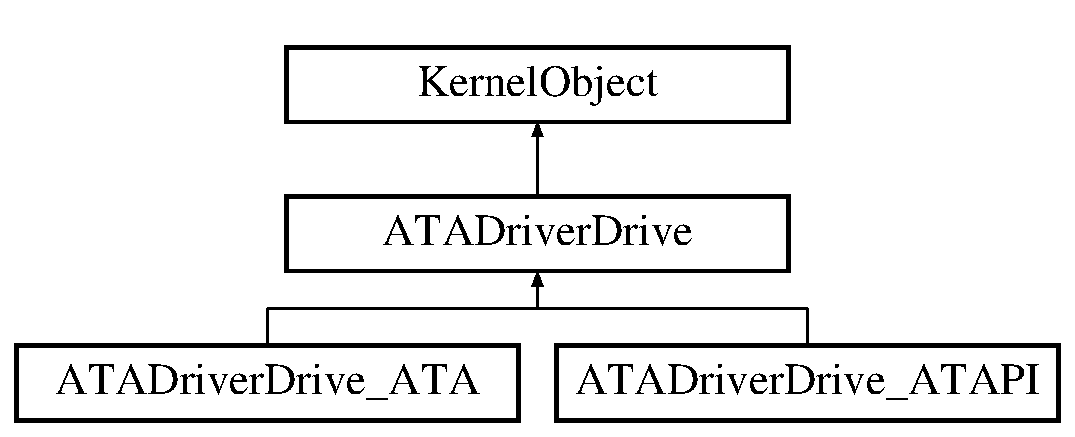
\includegraphics[height=3.000000cm]{class_a_t_a_driver_drive}
\end{center}
\end{figure}
\subsection*{Classes}
\begin{DoxyCompactItemize}
\item 
class \hyperlink{class_a_t_a_driver_drive_1_1_connection_handler}{Connection\+Handler}
\item 
class \hyperlink{class_a_t_a_driver_drive_1_1_generic_handler}{Generic\+Handler}
\item 
class \hyperlink{class_a_t_a_driver_drive_1_1_request}{Request}
\item 
class \hyperlink{class_a_t_a_driver_drive_1_1_request_handler}{Request\+Handler}
\item 
class \hyperlink{class_a_t_a_driver_drive_1_1_response_helper}{Response\+Helper}
\end{DoxyCompactItemize}
\subsection*{Public Member Functions}
\begin{DoxyCompactItemize}
\item 
\mbox{\Hypertarget{class_a_t_a_driver_drive_a2dff4ce26285788b53eca58d90805377}\label{class_a_t_a_driver_drive_a2dff4ce26285788b53eca58d90805377}} 
const char $\ast$ {\bfseries Get\+Class\+Name} (U\+Int32 level)
\item 
\mbox{\Hypertarget{class_a_t_a_driver_drive_a2285e89405b4ee1713f33764a8dc7a6f}\label{class_a_t_a_driver_drive_a2285e89405b4ee1713f33764a8dc7a6f}} 
{\bfseries A\+T\+A\+Driver\+Drive} (\hyperlink{class_a_t_a_driver}{A\+T\+A\+Driver} $\ast$driver, const char $\ast$mode, int index, \hyperlink{class_dispatch_queue}{Dispatch\+Queue} $\ast$queue)
\item 
\mbox{\Hypertarget{class_a_t_a_driver_drive_adec8a8a45d54b04b934b83635ab7c024}\label{class_a_t_a_driver_drive_adec8a8a45d54b04b934b83635ab7c024}} 
void {\bfseries Incoming\+Connection} (void)
\item 
\mbox{\Hypertarget{class_a_t_a_driver_drive_a320e2ce5cb415ca2774e09599594ded7}\label{class_a_t_a_driver_drive_a320e2ce5cb415ca2774e09599594ded7}} 
void {\bfseries Received\+Request} (\hyperlink{class_ipc_endpoint}{Ipc\+Endpoint} $\ast$connection)
\item 
\mbox{\Hypertarget{class_a_t_a_driver_drive_a6634cf8a9efd443ca199418eb4206a27}\label{class_a_t_a_driver_drive_a6634cf8a9efd443ca199418eb4206a27}} 
virtual void {\bfseries Process\+Request} (\hyperlink{class_ipc_endpoint}{Ipc\+Endpoint} $\ast$endpoint, Block\+Request $\ast$request, U\+Int64 length)=0
\end{DoxyCompactItemize}
\subsection*{Public Attributes}
\begin{DoxyCompactItemize}
\item 
\mbox{\Hypertarget{class_a_t_a_driver_drive_af6e820666a196d72e551110840d97556}\label{class_a_t_a_driver_drive_af6e820666a196d72e551110840d97556}} 
\hyperlink{class_ipc_service}{Ipc\+Service} $\ast$ {\bfseries \+\_\+service}
\end{DoxyCompactItemize}
\subsection*{Protected Attributes}
\begin{DoxyCompactItemize}
\item 
\mbox{\Hypertarget{class_a_t_a_driver_drive_aa880819cc83891928b099d242aa41591}\label{class_a_t_a_driver_drive_aa880819cc83891928b099d242aa41591}} 
\hyperlink{class_a_t_a_driver}{A\+T\+A\+Driver} $\ast$ {\bfseries \+\_\+driver}
\item 
\mbox{\Hypertarget{class_a_t_a_driver_drive_a93a8d1eb7eab06302e2662985bfca604}\label{class_a_t_a_driver_drive_a93a8d1eb7eab06302e2662985bfca604}} 
U\+Int32 {\bfseries \+\_\+driver\+Index}
\item 
\mbox{\Hypertarget{class_a_t_a_driver_drive_a72ee849627a09af62a58dce5bdee7a7e}\label{class_a_t_a_driver_drive_a72ee849627a09af62a58dce5bdee7a7e}} 
U\+Int16 {\bfseries \+\_\+sector\+Size}
\end{DoxyCompactItemize}
\subsection*{Private Attributes}
\begin{DoxyCompactItemize}
\item 
\mbox{\Hypertarget{class_a_t_a_driver_drive_aa3cea150d3b22e5ceeb617ed841c8bf5}\label{class_a_t_a_driver_drive_aa3cea150d3b22e5ceeb617ed841c8bf5}} 
\hyperlink{class_dispatch_queue}{Dispatch\+Queue} $\ast$ {\bfseries \+\_\+queue}
\end{DoxyCompactItemize}
\subsection*{Additional Inherited Members}


The documentation for this class was generated from the following file\+:\begin{DoxyCompactItemize}
\item 
Driver\+\_\+\+A\+T\+A.\+cpp\end{DoxyCompactItemize}

\hypertarget{class_a_t_a_driver_drive___a_t_a}{}\section{A\+T\+A\+Driver\+Drive\+\_\+\+A\+TA Class Reference}
\label{class_a_t_a_driver_drive___a_t_a}\index{A\+T\+A\+Driver\+Drive\+\_\+\+A\+TA@{A\+T\+A\+Driver\+Drive\+\_\+\+A\+TA}}
Inheritance diagram for A\+T\+A\+Driver\+Drive\+\_\+\+A\+TA\+:\begin{figure}[H]
\begin{center}
\leavevmode
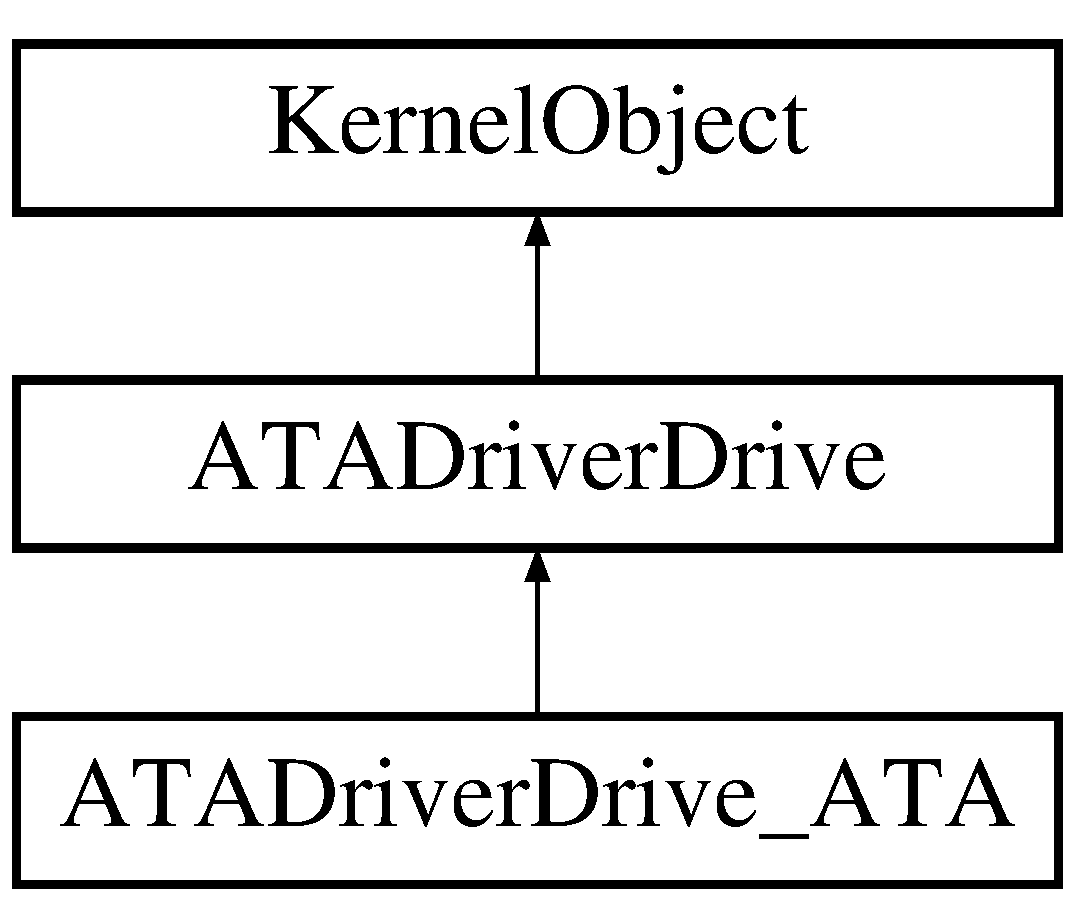
\includegraphics[height=3.000000cm]{class_a_t_a_driver_drive___a_t_a}
\end{center}
\end{figure}
\subsection*{Public Member Functions}
\begin{DoxyCompactItemize}
\item 
\mbox{\Hypertarget{class_a_t_a_driver_drive___a_t_a_aebd5ce9d0b960c477c5016e5c1875cae}\label{class_a_t_a_driver_drive___a_t_a_aebd5ce9d0b960c477c5016e5c1875cae}} 
const char $\ast$ {\bfseries Get\+Class\+Name} (U\+Int32 level)
\item 
\mbox{\Hypertarget{class_a_t_a_driver_drive___a_t_a_aea19e3107997411345a133c4a9ac5fe3}\label{class_a_t_a_driver_drive___a_t_a_aea19e3107997411345a133c4a9ac5fe3}} 
{\bfseries A\+T\+A\+Driver\+Drive\+\_\+\+A\+TA} (\hyperlink{class_a_t_a_driver}{A\+T\+A\+Driver} $\ast$driver, int index, \hyperlink{class_dispatch_queue}{Dispatch\+Queue} $\ast$queue)
\item 
\mbox{\Hypertarget{class_a_t_a_driver_drive___a_t_a_a630b62e187dd6eb85c69c85c0ec5ce3d}\label{class_a_t_a_driver_drive___a_t_a_a630b62e187dd6eb85c69c85c0ec5ce3d}} 
void {\bfseries Process\+Request} (\hyperlink{class_ipc_endpoint}{Ipc\+Endpoint} $\ast$endpoint, Block\+Request $\ast$request, U\+Int64 length)
\end{DoxyCompactItemize}
\subsection*{Additional Inherited Members}


The documentation for this class was generated from the following file\+:\begin{DoxyCompactItemize}
\item 
Driver\+\_\+\+A\+T\+A.\+cpp\end{DoxyCompactItemize}

\hypertarget{class_a_t_a_driver_drive___a_t_a_p_i}{}\section{A\+T\+A\+Driver\+Drive\+\_\+\+A\+T\+A\+PI Class Reference}
\label{class_a_t_a_driver_drive___a_t_a_p_i}\index{A\+T\+A\+Driver\+Drive\+\_\+\+A\+T\+A\+PI@{A\+T\+A\+Driver\+Drive\+\_\+\+A\+T\+A\+PI}}
Inheritance diagram for A\+T\+A\+Driver\+Drive\+\_\+\+A\+T\+A\+PI\+:\begin{figure}[H]
\begin{center}
\leavevmode
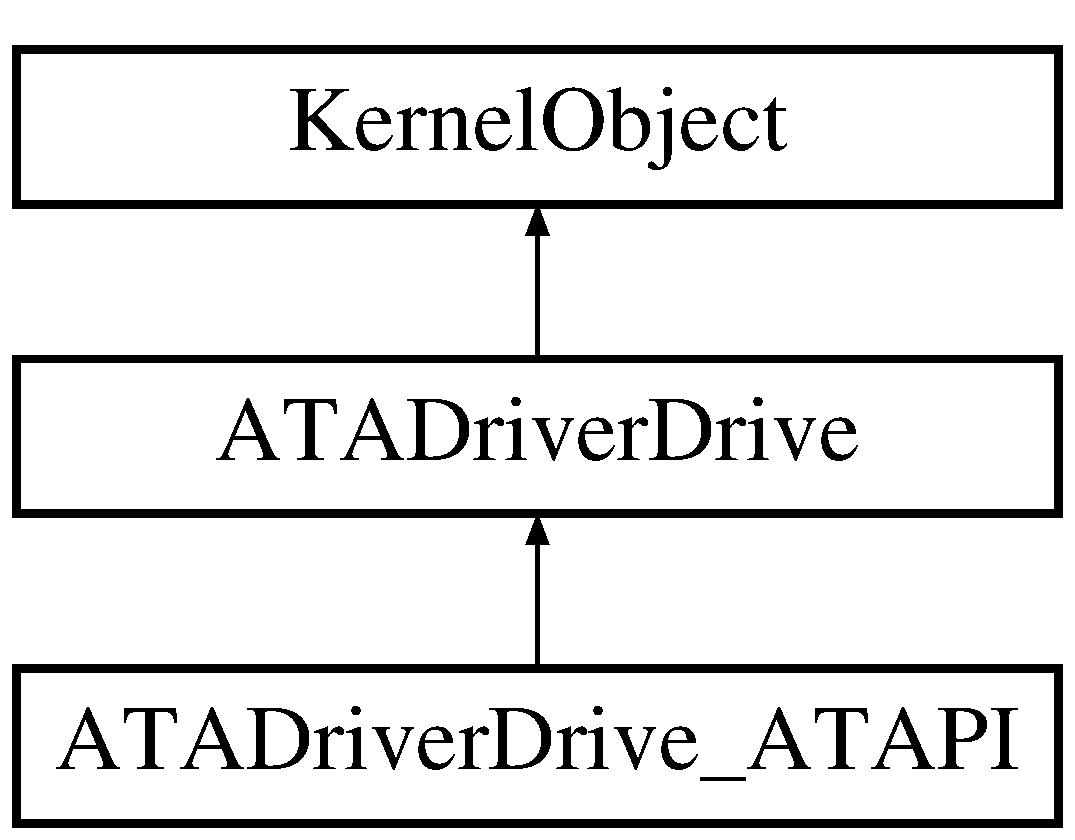
\includegraphics[height=3.000000cm]{class_a_t_a_driver_drive___a_t_a_p_i}
\end{center}
\end{figure}
\subsection*{Public Member Functions}
\begin{DoxyCompactItemize}
\item 
\mbox{\Hypertarget{class_a_t_a_driver_drive___a_t_a_p_i_a53892ccf58c952b1b670e6d41bcf32c8}\label{class_a_t_a_driver_drive___a_t_a_p_i_a53892ccf58c952b1b670e6d41bcf32c8}} 
const char $\ast$ {\bfseries Get\+Class\+Name} (U\+Int32 level)
\item 
\mbox{\Hypertarget{class_a_t_a_driver_drive___a_t_a_p_i_a9a12fbb0c92d9483c2dc17528e3eecf0}\label{class_a_t_a_driver_drive___a_t_a_p_i_a9a12fbb0c92d9483c2dc17528e3eecf0}} 
{\bfseries A\+T\+A\+Driver\+Drive\+\_\+\+A\+T\+A\+PI} (\hyperlink{class_a_t_a_driver}{A\+T\+A\+Driver} $\ast$driver, int index, \hyperlink{class_dispatch_queue}{Dispatch\+Queue} $\ast$queue)
\item 
\mbox{\Hypertarget{class_a_t_a_driver_drive___a_t_a_p_i_ae44b8c13d9be2b3b6fbbba4e29f7b3b4}\label{class_a_t_a_driver_drive___a_t_a_p_i_ae44b8c13d9be2b3b6fbbba4e29f7b3b4}} 
void {\bfseries Process\+Request} (\hyperlink{class_ipc_endpoint}{Ipc\+Endpoint} $\ast$endpoint, Block\+Request $\ast$request, U\+Int64 length)
\end{DoxyCompactItemize}
\subsection*{Additional Inherited Members}


The documentation for this class was generated from the following file\+:\begin{DoxyCompactItemize}
\item 
Driver\+\_\+\+A\+T\+A.\+cpp\end{DoxyCompactItemize}

\hypertarget{class_a_t_a_driver_node}{}\section{A\+T\+A\+Driver\+Node Class Reference}
\label{class_a_t_a_driver_node}\index{A\+T\+A\+Driver\+Node@{A\+T\+A\+Driver\+Node}}
Inheritance diagram for A\+T\+A\+Driver\+Node\+:\begin{figure}[H]
\begin{center}
\leavevmode
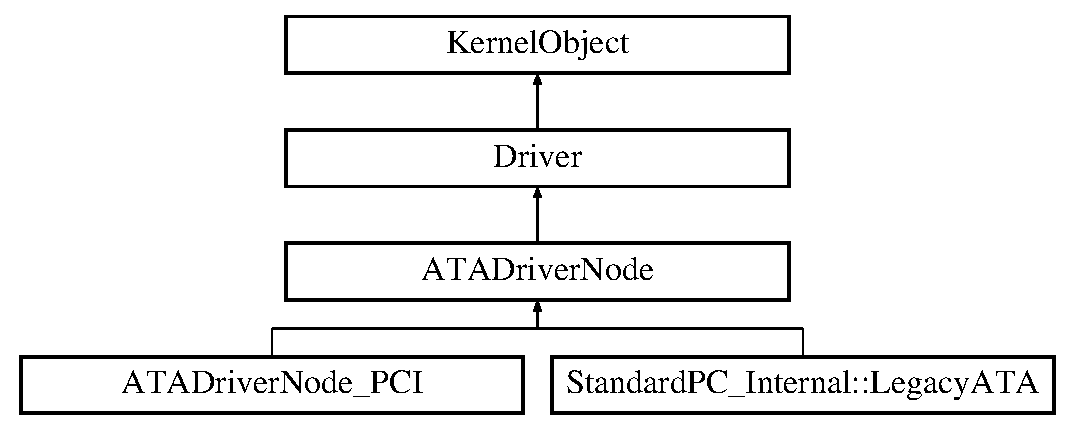
\includegraphics[height=4.000000cm]{class_a_t_a_driver_node}
\end{center}
\end{figure}
\subsection*{Public Member Functions}
\begin{DoxyCompactItemize}
\item 
\mbox{\Hypertarget{class_a_t_a_driver_node_a62e908c3ad6855e40a9e3f922ebd49d4}\label{class_a_t_a_driver_node_a62e908c3ad6855e40a9e3f922ebd49d4}} 
const char $\ast$ {\bfseries Get\+Class\+Name} (U\+Int32 level)
\item 
\mbox{\Hypertarget{class_a_t_a_driver_node_ac79dac66865a1b0ac13ea55d0b99f1c3}\label{class_a_t_a_driver_node_ac79dac66865a1b0ac13ea55d0b99f1c3}} 
{\bfseries A\+T\+A\+Driver\+Node} (const char $\ast$name)
\item 
\mbox{\Hypertarget{class_a_t_a_driver_node_a2022fc6685c72d9580a1afa878470cda}\label{class_a_t_a_driver_node_a2022fc6685c72d9580a1afa878470cda}} 
virtual U\+Int8 {\bfseries in\+Byte} (U\+Int32 address)=0
\item 
\mbox{\Hypertarget{class_a_t_a_driver_node_a3edab33f667a6033e93f1a627e5b54cc}\label{class_a_t_a_driver_node_a3edab33f667a6033e93f1a627e5b54cc}} 
virtual U\+Int16 {\bfseries in\+Short} (U\+Int32 address)=0
\item 
\mbox{\Hypertarget{class_a_t_a_driver_node_afb23a527dfddffab2773cbca507bdf95}\label{class_a_t_a_driver_node_afb23a527dfddffab2773cbca507bdf95}} 
virtual U\+Int32 {\bfseries in\+Long} (U\+Int32 address)=0
\item 
\mbox{\Hypertarget{class_a_t_a_driver_node_aceea9742a57fe02bebace6822330fec1}\label{class_a_t_a_driver_node_aceea9742a57fe02bebace6822330fec1}} 
virtual void {\bfseries out\+Byte} (U\+Int32 address, U\+Int8 byte)=0
\item 
\mbox{\Hypertarget{class_a_t_a_driver_node_ae3f04adeed8ec66ec0a335c53245dec4}\label{class_a_t_a_driver_node_ae3f04adeed8ec66ec0a335c53245dec4}} 
virtual void {\bfseries out\+Short} (U\+Int32 address, U\+Int16 byte)=0
\item 
\mbox{\Hypertarget{class_a_t_a_driver_node_a336a09330409830b3e22e9d2216f7543}\label{class_a_t_a_driver_node_a336a09330409830b3e22e9d2216f7543}} 
virtual void {\bfseries out\+Long} (U\+Int32 address, U\+Int32 byte)=0
\item 
\mbox{\Hypertarget{class_a_t_a_driver_node_a83481a2921bdd71dcd86fb97fd870d17}\label{class_a_t_a_driver_node_a83481a2921bdd71dcd86fb97fd870d17}} 
virtual void {\bfseries in\+Byte\+Rep} (U\+Int32 address, void $\ast$buffer, U\+Int32 length)=0
\item 
\mbox{\Hypertarget{class_a_t_a_driver_node_af82e63d322aa2e93ff1c7326eb4946c8}\label{class_a_t_a_driver_node_af82e63d322aa2e93ff1c7326eb4946c8}} 
virtual void {\bfseries in\+Short\+Rep} (U\+Int32 address, void $\ast$buffer, U\+Int32 length)=0
\item 
\mbox{\Hypertarget{class_a_t_a_driver_node_ab0e5bb5348c9f3f512a48fd48821ce7d}\label{class_a_t_a_driver_node_ab0e5bb5348c9f3f512a48fd48821ce7d}} 
virtual void {\bfseries in\+Long\+Rep} (U\+Int32 address, void $\ast$buffer, U\+Int32 length)=0
\item 
\mbox{\Hypertarget{class_a_t_a_driver_node_ac44712ba1cec68e5af518bbe7ab52ca2}\label{class_a_t_a_driver_node_ac44712ba1cec68e5af518bbe7ab52ca2}} 
virtual void {\bfseries out\+Byte\+Rep} (U\+Int32 address, void $\ast$buffer, U\+Int32 length)=0
\item 
\mbox{\Hypertarget{class_a_t_a_driver_node_a40111b18b03dfb80428bcd9f2434e004}\label{class_a_t_a_driver_node_a40111b18b03dfb80428bcd9f2434e004}} 
virtual void {\bfseries out\+Short\+Rep} (U\+Int32 address, void $\ast$buffer, U\+Int32 length)=0
\item 
\mbox{\Hypertarget{class_a_t_a_driver_node_a9b078d6ee5c6a3282a4a27e62f56070b}\label{class_a_t_a_driver_node_a9b078d6ee5c6a3282a4a27e62f56070b}} 
virtual void {\bfseries out\+Long\+Rep} (U\+Int32 address, void $\ast$buffer, U\+Int32 length)=0
\item 
\mbox{\Hypertarget{class_a_t_a_driver_node_a78e6b31ebb2e275dd2fb9bb49a10588d}\label{class_a_t_a_driver_node_a78e6b31ebb2e275dd2fb9bb49a10588d}} 
virtual \hyperlink{class_blockable_object}{Blockable\+Object} $\ast$ {\bfseries Interrupt} (void)=0
\item 
\mbox{\Hypertarget{class_a_t_a_driver_node_a5a7a31265883f8371a13d3426fb6add4}\label{class_a_t_a_driver_node_a5a7a31265883f8371a13d3426fb6add4}} 
virtual void {\bfseries Reset\+Interrupt} (void)=0
\item 
\mbox{\Hypertarget{class_a_t_a_driver_node_a2a44b1948f7aa7ddfb2d36013b56b8b8}\label{class_a_t_a_driver_node_a2a44b1948f7aa7ddfb2d36013b56b8b8}} 
U\+Int8 {\bfseries Interrupt\+Status} (void)
\item 
\mbox{\Hypertarget{class_a_t_a_driver_node_ac46d045009a24165081e8268b6c472ef}\label{class_a_t_a_driver_node_ac46d045009a24165081e8268b6c472ef}} 
U\+Int8 {\bfseries B\+M\+I\+D\+E\+Status} (void)
\item 
\mbox{\Hypertarget{class_a_t_a_driver_node_a2867a9c523be6e53f3b2b2828db351ff}\label{class_a_t_a_driver_node_a2867a9c523be6e53f3b2b2828db351ff}} 
void {\bfseries Update\+B\+M\+I\+D\+E\+State} (void)
\item 
\mbox{\Hypertarget{class_a_t_a_driver_node_aa2a9cb6f18a21ffa7ac059b271d1bb9f}\label{class_a_t_a_driver_node_aa2a9cb6f18a21ffa7ac059b271d1bb9f}} 
virtual bool {\bfseries D\+M\+A\+Available} (void)=0
\item 
\mbox{\Hypertarget{class_a_t_a_driver_node_a507da936d6bcce3fc41b875699c12015}\label{class_a_t_a_driver_node_a507da936d6bcce3fc41b875699c12015}} 
virtual U\+Int8 {\bfseries read\+Bus\+Master\+Status} (void)=0
\item 
\mbox{\Hypertarget{class_a_t_a_driver_node_a95d650298bffca359cd9800ba0fb29b9}\label{class_a_t_a_driver_node_a95d650298bffca359cd9800ba0fb29b9}} 
virtual void {\bfseries write\+Bus\+Master\+Status} (U\+Int8 x)=0
\end{DoxyCompactItemize}
\subsection*{Protected Member Functions}
\begin{DoxyCompactItemize}
\item 
\mbox{\Hypertarget{class_a_t_a_driver_node_a59256e38b62527a4d3d56347c3048b34}\label{class_a_t_a_driver_node_a59256e38b62527a4d3d56347c3048b34}} 
bool {\bfseries Update\+For\+Interrupt} (void)
\end{DoxyCompactItemize}
\subsection*{Private Attributes}
\begin{DoxyCompactItemize}
\item 
\mbox{\Hypertarget{class_a_t_a_driver_node_ad0aa8b905e16b316ef54d32792479979}\label{class_a_t_a_driver_node_ad0aa8b905e16b316ef54d32792479979}} 
U\+Int8 {\bfseries \+\_\+interrupt\+Status}
\item 
\mbox{\Hypertarget{class_a_t_a_driver_node_a9d4da4f71c18023dba9536ef358ef97a}\label{class_a_t_a_driver_node_a9d4da4f71c18023dba9536ef358ef97a}} 
U\+Int8 {\bfseries \+\_\+bm\+Status}
\end{DoxyCompactItemize}
\subsection*{Additional Inherited Members}


The documentation for this class was generated from the following files\+:\begin{DoxyCompactItemize}
\item 
Driver\+\_\+\+A\+T\+A.\+h\item 
Driver\+\_\+\+A\+T\+A.\+cpp\end{DoxyCompactItemize}

\hypertarget{class_a_t_a_driver_node___p_c_i}{}\section{A\+T\+A\+Driver\+Node\+\_\+\+P\+CI Class Reference}
\label{class_a_t_a_driver_node___p_c_i}\index{A\+T\+A\+Driver\+Node\+\_\+\+P\+CI@{A\+T\+A\+Driver\+Node\+\_\+\+P\+CI}}
Inheritance diagram for A\+T\+A\+Driver\+Node\+\_\+\+P\+CI\+:\begin{figure}[H]
\begin{center}
\leavevmode
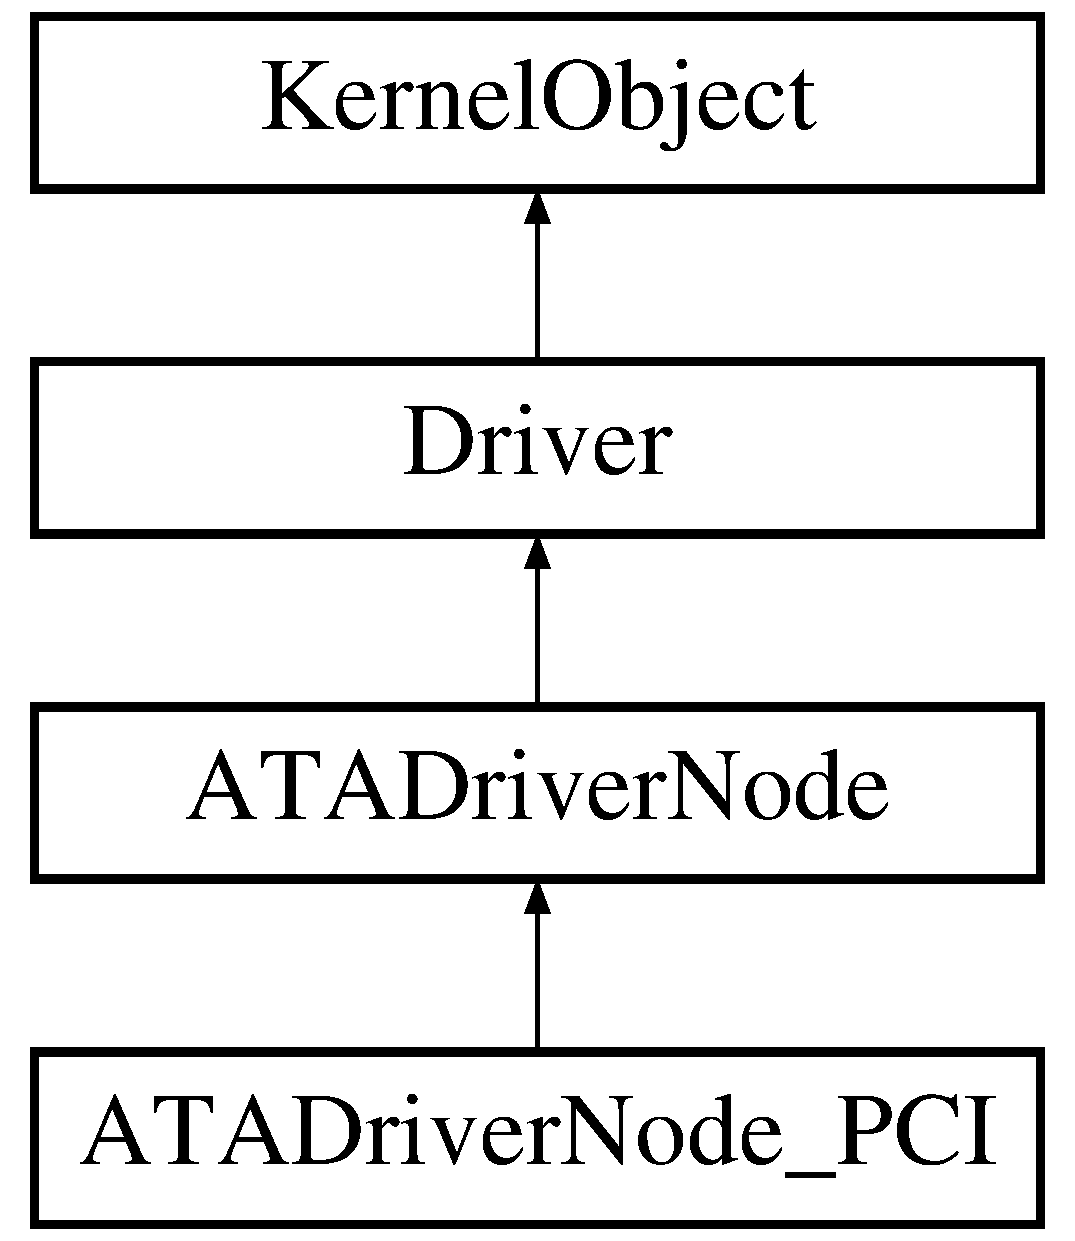
\includegraphics[height=4.000000cm]{class_a_t_a_driver_node___p_c_i}
\end{center}
\end{figure}
\subsection*{Classes}
\begin{DoxyCompactItemize}
\item 
class \hyperlink{class_a_t_a_driver_node___p_c_i_1_1_factory}{Factory}
\end{DoxyCompactItemize}
\subsection*{Public Member Functions}
\begin{DoxyCompactItemize}
\item 
\mbox{\Hypertarget{class_a_t_a_driver_node___p_c_i_a9ffff717b10d13bf6459bedaee3912e9}\label{class_a_t_a_driver_node___p_c_i_a9ffff717b10d13bf6459bedaee3912e9}} 
const char $\ast$ {\bfseries Get\+Class\+Name} (U\+Int32 level)
\item 
\mbox{\Hypertarget{class_a_t_a_driver_node___p_c_i_ab53db87dd2c34fe6bd9c3285945c9a3d}\label{class_a_t_a_driver_node___p_c_i_ab53db87dd2c34fe6bd9c3285945c9a3d}} 
{\bfseries A\+T\+A\+Driver\+Node\+\_\+\+P\+CI} (bool primary)
\item 
\mbox{\Hypertarget{class_a_t_a_driver_node___p_c_i_ab683ba5ad25993c17e129400379f3a77}\label{class_a_t_a_driver_node___p_c_i_ab683ba5ad25993c17e129400379f3a77}} 
bool {\bfseries Start} (\hyperlink{class_driver}{Driver} $\ast$parent)
\item 
\mbox{\Hypertarget{class_a_t_a_driver_node___p_c_i_a390a544ec824d21aff0338f1c742b18f}\label{class_a_t_a_driver_node___p_c_i_a390a544ec824d21aff0338f1c742b18f}} 
void {\bfseries Stop} (void)
\item 
\mbox{\Hypertarget{class_a_t_a_driver_node___p_c_i_a38d02cbce526950bb2dbfc602567e56d}\label{class_a_t_a_driver_node___p_c_i_a38d02cbce526950bb2dbfc602567e56d}} 
U\+Int8 {\bfseries in\+Byte} (U\+Int32 address)
\item 
\mbox{\Hypertarget{class_a_t_a_driver_node___p_c_i_a99a722f1bd82c4149657d74046451268}\label{class_a_t_a_driver_node___p_c_i_a99a722f1bd82c4149657d74046451268}} 
U\+Int16 {\bfseries in\+Short} (U\+Int32 address)
\item 
\mbox{\Hypertarget{class_a_t_a_driver_node___p_c_i_a12bdfd810a0cf2690a414544560df26b}\label{class_a_t_a_driver_node___p_c_i_a12bdfd810a0cf2690a414544560df26b}} 
U\+Int32 {\bfseries in\+Long} (U\+Int32 address)
\item 
\mbox{\Hypertarget{class_a_t_a_driver_node___p_c_i_a7edd942b48f5e6508b7485f40ac5d1ad}\label{class_a_t_a_driver_node___p_c_i_a7edd942b48f5e6508b7485f40ac5d1ad}} 
void {\bfseries out\+Byte} (U\+Int32 address, U\+Int8 byte)
\item 
\mbox{\Hypertarget{class_a_t_a_driver_node___p_c_i_a9746c4e2ef2a10fbaacfc06ad9b9203c}\label{class_a_t_a_driver_node___p_c_i_a9746c4e2ef2a10fbaacfc06ad9b9203c}} 
void {\bfseries out\+Short} (U\+Int32 address, U\+Int16 byte)
\item 
\mbox{\Hypertarget{class_a_t_a_driver_node___p_c_i_a378a53cc83790ba2c5991b28587f1dc2}\label{class_a_t_a_driver_node___p_c_i_a378a53cc83790ba2c5991b28587f1dc2}} 
void {\bfseries out\+Long} (U\+Int32 address, U\+Int32 byte)
\item 
\mbox{\Hypertarget{class_a_t_a_driver_node___p_c_i_a7a44c25032f56987a24038b1a09df602}\label{class_a_t_a_driver_node___p_c_i_a7a44c25032f56987a24038b1a09df602}} 
void {\bfseries in\+Byte\+Rep} (U\+Int32 address, void $\ast$buffer, U\+Int32 length)
\item 
\mbox{\Hypertarget{class_a_t_a_driver_node___p_c_i_ad32d892b3955c8bbcd29ad5bdf7f6174}\label{class_a_t_a_driver_node___p_c_i_ad32d892b3955c8bbcd29ad5bdf7f6174}} 
void {\bfseries in\+Short\+Rep} (U\+Int32 address, void $\ast$buffer, U\+Int32 length)
\item 
\mbox{\Hypertarget{class_a_t_a_driver_node___p_c_i_ae52364b6780b52da18b066e00ee2f062}\label{class_a_t_a_driver_node___p_c_i_ae52364b6780b52da18b066e00ee2f062}} 
void {\bfseries in\+Long\+Rep} (U\+Int32 address, void $\ast$buffer, U\+Int32 length)
\item 
\mbox{\Hypertarget{class_a_t_a_driver_node___p_c_i_a0c93318ee575386ccfe0f8abfb0d7b53}\label{class_a_t_a_driver_node___p_c_i_a0c93318ee575386ccfe0f8abfb0d7b53}} 
void {\bfseries out\+Byte\+Rep} (U\+Int32 address, void $\ast$buffer, U\+Int32 length)
\item 
\mbox{\Hypertarget{class_a_t_a_driver_node___p_c_i_a91715178936488341c6b85f616b5f68a}\label{class_a_t_a_driver_node___p_c_i_a91715178936488341c6b85f616b5f68a}} 
void {\bfseries out\+Short\+Rep} (U\+Int32 address, void $\ast$buffer, U\+Int32 length)
\item 
\mbox{\Hypertarget{class_a_t_a_driver_node___p_c_i_ac03497012e6c8778e0da03e727370fb9}\label{class_a_t_a_driver_node___p_c_i_ac03497012e6c8778e0da03e727370fb9}} 
void {\bfseries out\+Long\+Rep} (U\+Int32 address, void $\ast$buffer, U\+Int32 length)
\item 
\mbox{\Hypertarget{class_a_t_a_driver_node___p_c_i_acfe6c674f857bd166f4c30317a062041}\label{class_a_t_a_driver_node___p_c_i_acfe6c674f857bd166f4c30317a062041}} 
\hyperlink{class_blockable_object}{Blockable\+Object} $\ast$ {\bfseries Interrupt} (void)
\item 
\mbox{\Hypertarget{class_a_t_a_driver_node___p_c_i_a8e1814f837bd766c3aa4c6aca0353f9f}\label{class_a_t_a_driver_node___p_c_i_a8e1814f837bd766c3aa4c6aca0353f9f}} 
void {\bfseries Reset\+Interrupt} (void)
\item 
\mbox{\Hypertarget{class_a_t_a_driver_node___p_c_i_a3e8d76e23a4858280ab1b0bcc935d3c4}\label{class_a_t_a_driver_node___p_c_i_a3e8d76e23a4858280ab1b0bcc935d3c4}} 
bool {\bfseries D\+M\+A\+Available} (void)
\item 
\mbox{\Hypertarget{class_a_t_a_driver_node___p_c_i_a8ea1f7fe16a942402b46ac65e5349522}\label{class_a_t_a_driver_node___p_c_i_a8ea1f7fe16a942402b46ac65e5349522}} 
U\+Int8 {\bfseries read\+Bus\+Master\+Status} (void)
\item 
\mbox{\Hypertarget{class_a_t_a_driver_node___p_c_i_a64ff7d4170b18c49743ab195328b0eab}\label{class_a_t_a_driver_node___p_c_i_a64ff7d4170b18c49743ab195328b0eab}} 
void {\bfseries write\+Bus\+Master\+Status} (U\+Int8 x)
\end{DoxyCompactItemize}
\subsection*{Private Member Functions}
\begin{DoxyCompactItemize}
\item 
\mbox{\Hypertarget{class_a_t_a_driver_node___p_c_i_a1d7520ac832dcbd8a7d4b74a31c862b8}\label{class_a_t_a_driver_node___p_c_i_a1d7520ac832dcbd8a7d4b74a31c862b8}} 
U\+Int16 {\bfseries Get\+Port} (U\+Int32 address)
\end{DoxyCompactItemize}
\subsection*{Private Attributes}
\begin{DoxyCompactItemize}
\item 
\mbox{\Hypertarget{class_a_t_a_driver_node___p_c_i_a9d5ddedaf82426be62dc1dd9c6cb8fa1}\label{class_a_t_a_driver_node___p_c_i_a9d5ddedaf82426be62dc1dd9c6cb8fa1}} 
bool {\bfseries \+\_\+primary}
\item 
\mbox{\Hypertarget{class_a_t_a_driver_node___p_c_i_adf530c62d89628ca43316a5004aa710c}\label{class_a_t_a_driver_node___p_c_i_adf530c62d89628ca43316a5004aa710c}} 
U\+Int32 {\bfseries \+\_\+io\+Port}
\item 
\mbox{\Hypertarget{class_a_t_a_driver_node___p_c_i_a7162b2098283f9a19ea38d8285ee6396}\label{class_a_t_a_driver_node___p_c_i_a7162b2098283f9a19ea38d8285ee6396}} 
U\+Int32 {\bfseries \+\_\+control\+Port}
\item 
\mbox{\Hypertarget{class_a_t_a_driver_node___p_c_i_a5e3ed984e876bc66dc895b40a6db70ae}\label{class_a_t_a_driver_node___p_c_i_a5e3ed984e876bc66dc895b40a6db70ae}} 
U\+Int32 {\bfseries \+\_\+bm\+Port}
\item 
\mbox{\Hypertarget{class_a_t_a_driver_node___p_c_i_a19ef9cef9b3eec0d968e00665534a190}\label{class_a_t_a_driver_node___p_c_i_a19ef9cef9b3eec0d968e00665534a190}} 
\hyperlink{class_simple_signal}{Simple\+Signal} $\ast$ {\bfseries \+\_\+interrupt}
\item 
\mbox{\Hypertarget{class_a_t_a_driver_node___p_c_i_a1f984269864e2349109732446229ef07}\label{class_a_t_a_driver_node___p_c_i_a1f984269864e2349109732446229ef07}} 
Interrupt\+Handler\+Handle {\bfseries \+\_\+interrupt\+Token}
\end{DoxyCompactItemize}
\subsection*{Additional Inherited Members}


The documentation for this class was generated from the following file\+:\begin{DoxyCompactItemize}
\item 
Driver\+\_\+\+A\+T\+A.\+cpp\end{DoxyCompactItemize}

\hypertarget{class_generic_lock_1_1_autolock}{}\section{Generic\+Lock\+:\+:Autolock Class Reference}
\label{class_generic_lock_1_1_autolock}\index{Generic\+Lock\+::\+Autolock@{Generic\+Lock\+::\+Autolock}}
\subsection*{Public Member Functions}
\begin{DoxyCompactItemize}
\item 
\mbox{\Hypertarget{class_generic_lock_1_1_autolock_a13d8fd8753758af8d01e70769223f040}\label{class_generic_lock_1_1_autolock_a13d8fd8753758af8d01e70769223f040}} 
{\bfseries Autolock} (\hyperlink{class_generic_lock}{Generic\+Lock} $\ast$lock)
\end{DoxyCompactItemize}
\subsection*{Private Attributes}
\begin{DoxyCompactItemize}
\item 
\mbox{\Hypertarget{class_generic_lock_1_1_autolock_af6542b5858c621e3e3425a4b5bf089dd}\label{class_generic_lock_1_1_autolock_af6542b5858c621e3e3425a4b5bf089dd}} 
\hyperlink{class_generic_lock}{Generic\+Lock} $\ast$ {\bfseries \+\_\+lock}
\end{DoxyCompactItemize}


The documentation for this class was generated from the following file\+:\begin{DoxyCompactItemize}
\item 
Locking.\+h\end{DoxyCompactItemize}

\hypertarget{class_uninterruptable_spin_lock_1_1_autolock}{}\section{Uninterruptable\+Spin\+Lock\+:\+:Autolock Class Reference}
\label{class_uninterruptable_spin_lock_1_1_autolock}\index{Uninterruptable\+Spin\+Lock\+::\+Autolock@{Uninterruptable\+Spin\+Lock\+::\+Autolock}}
\subsection*{Public Member Functions}
\begin{DoxyCompactItemize}
\item 
\mbox{\Hypertarget{class_uninterruptable_spin_lock_1_1_autolock_ae4929dda4d5292dbacaeb53989951ce7}\label{class_uninterruptable_spin_lock_1_1_autolock_ae4929dda4d5292dbacaeb53989951ce7}} 
{\bfseries Autolock} (\hyperlink{class_uninterruptable_spin_lock}{Uninterruptable\+Spin\+Lock} $\ast$lock)
\end{DoxyCompactItemize}
\subsection*{Private Attributes}
\begin{DoxyCompactItemize}
\item 
\mbox{\Hypertarget{class_uninterruptable_spin_lock_1_1_autolock_a5c3a2646096d5c130363e006c1da2113}\label{class_uninterruptable_spin_lock_1_1_autolock_a5c3a2646096d5c130363e006c1da2113}} 
\hyperlink{class_uninterruptable_spin_lock}{Uninterruptable\+Spin\+Lock} $\ast$ {\bfseries \+\_\+lock}
\end{DoxyCompactItemize}


The documentation for this class was generated from the following file\+:\begin{DoxyCompactItemize}
\item 
Locking.\+h\end{DoxyCompactItemize}

\hypertarget{class_interruptable_spin_lock_1_1_autolock}{}\section{Interruptable\+Spin\+Lock\+:\+:Autolock Class Reference}
\label{class_interruptable_spin_lock_1_1_autolock}\index{Interruptable\+Spin\+Lock\+::\+Autolock@{Interruptable\+Spin\+Lock\+::\+Autolock}}
\subsection*{Public Member Functions}
\begin{DoxyCompactItemize}
\item 
\mbox{\Hypertarget{class_interruptable_spin_lock_1_1_autolock_a468c166688de715f62f7075759c2dbf5}\label{class_interruptable_spin_lock_1_1_autolock_a468c166688de715f62f7075759c2dbf5}} 
{\bfseries Autolock} (\hyperlink{class_interruptable_spin_lock}{Interruptable\+Spin\+Lock} $\ast$lock)
\end{DoxyCompactItemize}
\subsection*{Private Attributes}
\begin{DoxyCompactItemize}
\item 
\mbox{\Hypertarget{class_interruptable_spin_lock_1_1_autolock_a11a887823f81d878af0e1c31cf765ed4}\label{class_interruptable_spin_lock_1_1_autolock_a11a887823f81d878af0e1c31cf765ed4}} 
\hyperlink{class_interruptable_spin_lock}{Interruptable\+Spin\+Lock} $\ast$ {\bfseries \+\_\+lock}
\end{DoxyCompactItemize}


The documentation for this class was generated from the following file\+:\begin{DoxyCompactItemize}
\item 
Locking.\+h\end{DoxyCompactItemize}

\hypertarget{class_autorelease_pool}{}\section{Autorelease\+Pool Class Reference}
\label{class_autorelease_pool}\index{Autorelease\+Pool@{Autorelease\+Pool}}
\subsection*{Public Member Functions}
\begin{DoxyCompactItemize}
\item 
\mbox{\Hypertarget{class_autorelease_pool_a0cb469d59376fef7cb5a822606af977f}\label{class_autorelease_pool_a0cb469d59376fef7cb5a822606af977f}} 
void {\bfseries Flush} (void)
\item 
\mbox{\Hypertarget{class_autorelease_pool_a240527d400e2f31879246667eea3bb1b}\label{class_autorelease_pool_a240527d400e2f31879246667eea3bb1b}} 
void {\bfseries Add\+Object} (\hyperlink{class_kernel_object}{Kernel\+Object} $\ast$object)
\end{DoxyCompactItemize}
\subsection*{Private Attributes}
\begin{DoxyCompactItemize}
\item 
\mbox{\Hypertarget{class_autorelease_pool_a35648f63c1f40ed7de9fe3e3d4d45145}\label{class_autorelease_pool_a35648f63c1f40ed7de9fe3e3d4d45145}} 
\hyperlink{class_kernel_array}{Kernel\+Array} $\ast$ {\bfseries \+\_\+objects}
\item 
\mbox{\Hypertarget{class_autorelease_pool_a07dd69f30cbaf1e8fb7c5f3b171c5100}\label{class_autorelease_pool_a07dd69f30cbaf1e8fb7c5f3b171c5100}} 
\hyperlink{class_autorelease_pool}{Autorelease\+Pool} $\ast$ {\bfseries \+\_\+previous}
\end{DoxyCompactItemize}


The documentation for this class was generated from the following files\+:\begin{DoxyCompactItemize}
\item 
Kernel\+Object.\+h\item 
Kernel\+Object.\+cpp\end{DoxyCompactItemize}

\hypertarget{class_autorelease_pool_wrapper}{}\section{Autorelease\+Pool\+Wrapper Class Reference}
\label{class_autorelease_pool_wrapper}\index{Autorelease\+Pool\+Wrapper@{Autorelease\+Pool\+Wrapper}}
Inheritance diagram for Autorelease\+Pool\+Wrapper\+:\begin{figure}[H]
\begin{center}
\leavevmode
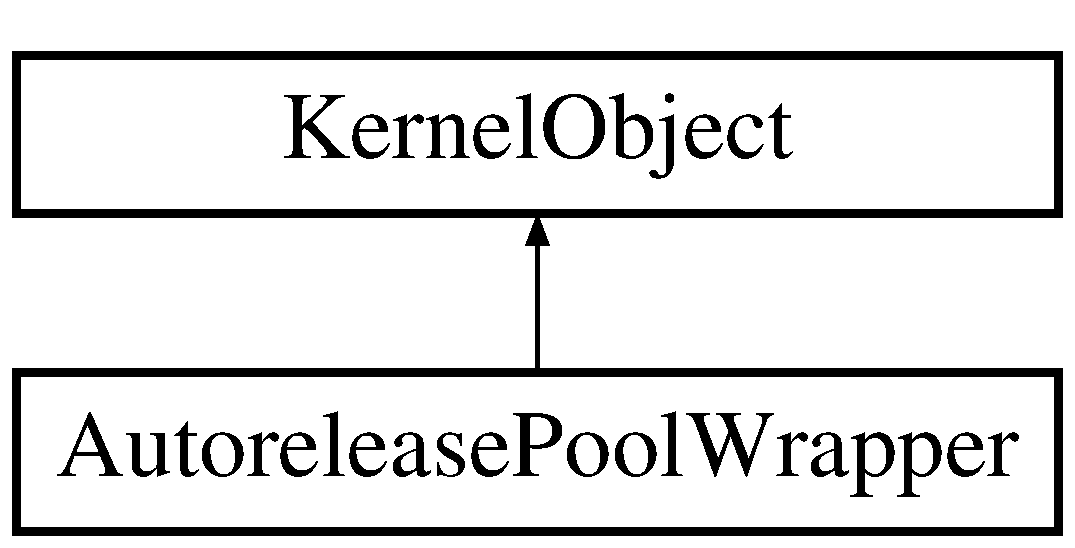
\includegraphics[height=2.000000cm]{class_autorelease_pool_wrapper}
\end{center}
\end{figure}
\subsection*{Public Member Functions}
\begin{DoxyCompactItemize}
\item 
\mbox{\Hypertarget{class_autorelease_pool_wrapper_a86606ece5fe2c12375f38b61c9dcd269}\label{class_autorelease_pool_wrapper_a86606ece5fe2c12375f38b61c9dcd269}} 
const char $\ast$ {\bfseries Get\+Class\+Name} (U\+Int32 level)
\item 
\mbox{\Hypertarget{class_autorelease_pool_wrapper_af78d131c8973ae5aae7e6ef1d6d91b4c}\label{class_autorelease_pool_wrapper_af78d131c8973ae5aae7e6ef1d6d91b4c}} 
{\bfseries Autorelease\+Pool\+Wrapper} (\hyperlink{class_autorelease_pool}{Autorelease\+Pool} $\ast$pool)
\end{DoxyCompactItemize}
\subsection*{Public Attributes}
\begin{DoxyCompactItemize}
\item 
\mbox{\Hypertarget{class_autorelease_pool_wrapper_a3ab16bc786d4319afbb09817b3d15a1c}\label{class_autorelease_pool_wrapper_a3ab16bc786d4319afbb09817b3d15a1c}} 
\hyperlink{class_autorelease_pool}{Autorelease\+Pool} $\ast$ {\bfseries \+\_\+pool}
\end{DoxyCompactItemize}
\subsection*{Additional Inherited Members}


The documentation for this class was generated from the following file\+:\begin{DoxyCompactItemize}
\item 
Kernel\+Object.\+cpp\end{DoxyCompactItemize}

\hypertarget{class_basic_heap}{}\section{Basic\+Heap Class Reference}
\label{class_basic_heap}\index{Basic\+Heap@{Basic\+Heap}}
\subsection*{Public Types}
\begin{DoxyCompactItemize}
\item 
\mbox{\Hypertarget{class_basic_heap_ab373b139903271cba9a74038376746dc}\label{class_basic_heap_ab373b139903271cba9a74038376746dc}} 
typedef unsigned long {\bfseries h\+\_\+size}
\end{DoxyCompactItemize}
\subsection*{Public Member Functions}
\begin{DoxyCompactItemize}
\item 
\mbox{\Hypertarget{class_basic_heap_a09729479676d8ccfb2fb59cb140a6aa9}\label{class_basic_heap_a09729479676d8ccfb2fb59cb140a6aa9}} 
void {\bfseries Add\+Block} (void $\ast$offset, h\+\_\+size length)
\item 
\mbox{\Hypertarget{class_basic_heap_a6227b3a159cf1769e8c758ee7abe1991}\label{class_basic_heap_a6227b3a159cf1769e8c758ee7abe1991}} 
void $\ast$ {\bfseries Alloc} (h\+\_\+size amount)
\item 
\mbox{\Hypertarget{class_basic_heap_a0ccbe7addeaf3f48971b810b595ac384}\label{class_basic_heap_a0ccbe7addeaf3f48971b810b595ac384}} 
void {\bfseries Release} (void $\ast$buffer)
\item 
\mbox{\Hypertarget{class_basic_heap_a85cda28f3010ea9224126f3e067f7c3e}\label{class_basic_heap_a85cda28f3010ea9224126f3e067f7c3e}} 
h\+\_\+size {\bfseries Total\+Memory} (void)
\item 
\mbox{\Hypertarget{class_basic_heap_a3fbb4aa5e17a3cdbeaff444b7022fd23}\label{class_basic_heap_a3fbb4aa5e17a3cdbeaff444b7022fd23}} 
h\+\_\+size {\bfseries Used\+Memory} (void)
\item 
\mbox{\Hypertarget{class_basic_heap_a3cb545adb35965285f84f2081a8da796}\label{class_basic_heap_a3cb545adb35965285f84f2081a8da796}} 
h\+\_\+size {\bfseries Free\+Memory} (void)
\item 
\mbox{\Hypertarget{class_basic_heap_aa4889e648609784e5dca60da308d50dd}\label{class_basic_heap_aa4889e648609784e5dca60da308d50dd}} 
h\+\_\+size {\bfseries Allocation\+Count} (void)
\item 
\mbox{\Hypertarget{class_basic_heap_abbef5717b4fd5d3f366bf89725671abe}\label{class_basic_heap_abbef5717b4fd5d3f366bf89725671abe}} 
void {\bfseries Test} (void)
\item 
\mbox{\Hypertarget{class_basic_heap_a1073a696e46034763b0c79306ba8b03d}\label{class_basic_heap_a1073a696e46034763b0c79306ba8b03d}} 
void {\bfseries Check} (void $\ast$)
\end{DoxyCompactItemize}
\subsection*{Private Attributes}
\begin{DoxyCompactItemize}
\item 
\mbox{\Hypertarget{class_basic_heap_afe5c9a65bbcb44b616b8db3ec422931e}\label{class_basic_heap_afe5c9a65bbcb44b616b8db3ec422931e}} 
\hyperlink{class_uninterruptable_spin_lock}{Uninterruptable\+Spin\+Lock} {\bfseries \+\_\+lock}
\item 
\mbox{\Hypertarget{class_basic_heap_a44e524a3f3699e0a323ff2d24a65cdf6}\label{class_basic_heap_a44e524a3f3699e0a323ff2d24a65cdf6}} 
\hyperlink{class_internal_1_1_free_space}{Internal\+::\+Free\+Space} $\ast$ {\bfseries \+\_\+free\+Start}
\item 
\mbox{\Hypertarget{class_basic_heap_acdc247c3c9a6056b9592ca61860888a5}\label{class_basic_heap_acdc247c3c9a6056b9592ca61860888a5}} 
\hyperlink{class_internal_1_1_free_space}{Internal\+::\+Free\+Space} $\ast$ {\bfseries \+\_\+free\+End}
\item 
\mbox{\Hypertarget{class_basic_heap_acbd2e99a996b5dc3bf52660545a93be1}\label{class_basic_heap_acbd2e99a996b5dc3bf52660545a93be1}} 
h\+\_\+size {\bfseries \+\_\+total}
\item 
\mbox{\Hypertarget{class_basic_heap_a88ebb1670a21c2dc251995486da321f0}\label{class_basic_heap_a88ebb1670a21c2dc251995486da321f0}} 
h\+\_\+size {\bfseries \+\_\+used}
\item 
\mbox{\Hypertarget{class_basic_heap_ae48f81b1c1d3e5d76441a6b3438c55de}\label{class_basic_heap_ae48f81b1c1d3e5d76441a6b3438c55de}} 
h\+\_\+size {\bfseries \+\_\+count}
\end{DoxyCompactItemize}
\subsection*{Friends}
\begin{DoxyCompactItemize}
\item 
\mbox{\Hypertarget{class_basic_heap_abcdce91148dce0245ab64ecb3763fccd}\label{class_basic_heap_abcdce91148dce0245ab64ecb3763fccd}} 
class {\bfseries Internal\+::\+Free\+Space}
\end{DoxyCompactItemize}


The documentation for this class was generated from the following files\+:\begin{DoxyCompactItemize}
\item 
Basic\+Heap.\+h\item 
Basic\+Heap.\+cpp\end{DoxyCompactItemize}

\hypertarget{class_binary_map}{}\section{Binary\+Map Class Reference}
\label{class_binary_map}\index{Binary\+Map@{Binary\+Map}}
Inheritance diagram for Binary\+Map\+:\begin{figure}[H]
\begin{center}
\leavevmode
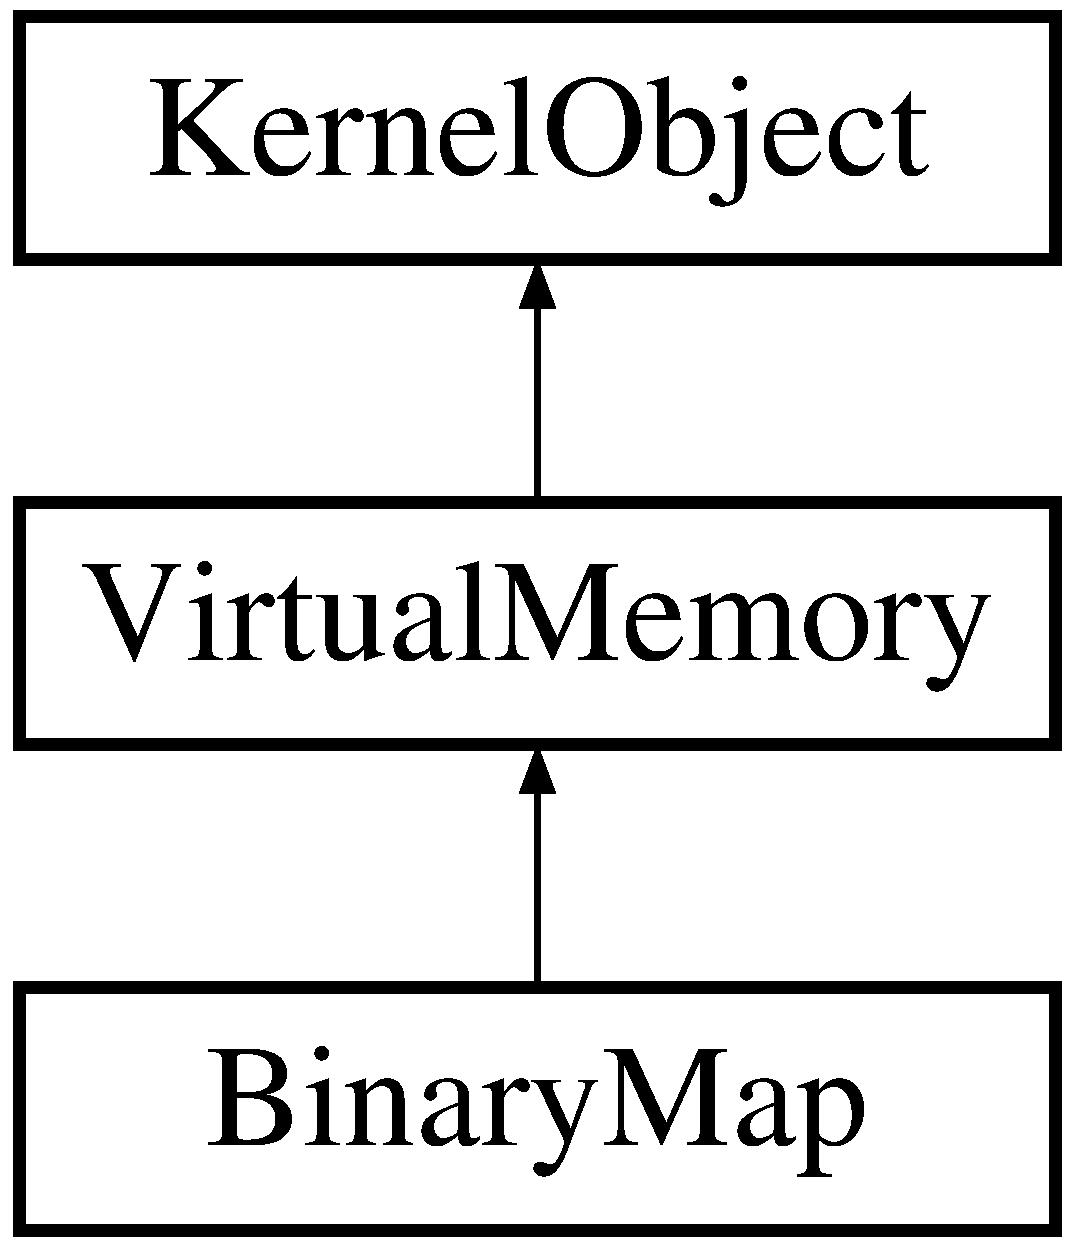
\includegraphics[height=3.000000cm]{class_binary_map}
\end{center}
\end{figure}
\subsection*{Public Member Functions}
\begin{DoxyCompactItemize}
\item 
\mbox{\Hypertarget{class_binary_map_af1dd6999b9654702d7a12310f0854d15}\label{class_binary_map_af1dd6999b9654702d7a12310f0854d15}} 
const char $\ast$ {\bfseries Get\+Class\+Name} (U\+Int32 level)
\item 
\mbox{\Hypertarget{class_binary_map_a712e67a9b086c0978216c6dadd1ba013}\label{class_binary_map_a712e67a9b086c0978216c6dadd1ba013}} 
{\bfseries Binary\+Map} (\hyperlink{class_process}{Process} $\ast$process, \hyperlink{class_interface_helper}{Interface\+Helper} $\ast$helper, \hyperlink{class_ipc_endpoint}{Ipc\+Endpoint} $\ast$connection, U\+Int32 chunk, U\+Int32 length)
\item 
\mbox{\Hypertarget{class_binary_map_ac1d23ebb9816d0e5b38f45d96df950ee}\label{class_binary_map_ac1d23ebb9816d0e5b38f45d96df950ee}} 
{\bfseries Binary\+Map} (\hyperlink{class_process}{Process} $\ast$process, \hyperlink{class_interface_helper}{Interface\+Helper} $\ast$helper, \hyperlink{class_ipc_endpoint}{Ipc\+Endpoint} $\ast$connection, U\+Int32 chunk, void $\ast$linear\+Base, U\+Int32 length)
\end{DoxyCompactItemize}
\subsection*{Protected Member Functions}
\begin{DoxyCompactItemize}
\item 
\mbox{\Hypertarget{class_binary_map_a2c58d83d15b26cb74bda9ac5b2e88e83}\label{class_binary_map_a2c58d83d15b26cb74bda9ac5b2e88e83}} 
void {\bfseries Handle\+Page\+Fault} (void $\ast$linear\+Address)
\end{DoxyCompactItemize}
\subsection*{Private Attributes}
\begin{DoxyCompactItemize}
\item 
\mbox{\Hypertarget{class_binary_map_aa0a1044f0f0262e7651ca196447c66e6}\label{class_binary_map_aa0a1044f0f0262e7651ca196447c66e6}} 
\hyperlink{class_interface_helper}{Interface\+Helper} $\ast$ {\bfseries \+\_\+owner\+Helper}
\item 
\mbox{\Hypertarget{class_binary_map_a24e66d94a55bae51d048fc0e691f4f72}\label{class_binary_map_a24e66d94a55bae51d048fc0e691f4f72}} 
\hyperlink{class_ipc_endpoint}{Ipc\+Endpoint} $\ast$ {\bfseries \+\_\+owner\+Connection}
\item 
\mbox{\Hypertarget{class_binary_map_ab80baabca4a1072238ad30f57e9bc6ea}\label{class_binary_map_ab80baabca4a1072238ad30f57e9bc6ea}} 
U\+Int32 {\bfseries \+\_\+chunk}
\end{DoxyCompactItemize}
\subsection*{Additional Inherited Members}


The documentation for this class was generated from the following file\+:\begin{DoxyCompactItemize}
\item 
Process.\+cpp\end{DoxyCompactItemize}

\hypertarget{class_test_harness_1_1_blob}{}\section{Test\+Harness\+:\+:Blob Class Reference}
\label{class_test_harness_1_1_blob}\index{Test\+Harness\+::\+Blob@{Test\+Harness\+::\+Blob}}
\subsection*{Public Member Functions}
\begin{DoxyCompactItemize}
\item 
\mbox{\Hypertarget{class_test_harness_1_1_blob_aa995eab940e164b12b1b286cdb110be8}\label{class_test_harness_1_1_blob_aa995eab940e164b12b1b286cdb110be8}} 
{\bfseries Blob} (\hyperlink{class_test_harness_1_1_blob}{Blob} $\ast$$\ast$start, \hyperlink{class_test_harness_1_1_blob}{Blob} $\ast$$\ast$end, void $\ast$offset, Basic\+Heap\+::h\+\_\+size length)
\end{DoxyCompactItemize}
\subsection*{Public Attributes}
\begin{DoxyCompactItemize}
\item 
\mbox{\Hypertarget{class_test_harness_1_1_blob_ac173605060f623f8b2be99e393c89096}\label{class_test_harness_1_1_blob_ac173605060f623f8b2be99e393c89096}} 
char $\ast$ {\bfseries \+\_\+offset}
\item 
\mbox{\Hypertarget{class_test_harness_1_1_blob_aa78c6c072eeaaa76d7445b3dce0cf4c8}\label{class_test_harness_1_1_blob_aa78c6c072eeaaa76d7445b3dce0cf4c8}} 
Basic\+Heap\+::h\+\_\+size {\bfseries \+\_\+length}
\item 
\mbox{\Hypertarget{class_test_harness_1_1_blob_a13c66a59433a68cbc918987d8cc71e84}\label{class_test_harness_1_1_blob_a13c66a59433a68cbc918987d8cc71e84}} 
\hyperlink{class_test_harness_1_1_blob}{Blob} $\ast$$\ast$ {\bfseries \+\_\+start}
\item 
\mbox{\Hypertarget{class_test_harness_1_1_blob_a99c2c5cdaf01a9ff1d9cd4ebd7888bf9}\label{class_test_harness_1_1_blob_a99c2c5cdaf01a9ff1d9cd4ebd7888bf9}} 
\hyperlink{class_test_harness_1_1_blob}{Blob} $\ast$$\ast$ {\bfseries \+\_\+end}
\item 
\mbox{\Hypertarget{class_test_harness_1_1_blob_ae4967f6930a3e41d4005a3a6ae773422}\label{class_test_harness_1_1_blob_ae4967f6930a3e41d4005a3a6ae773422}} 
\hyperlink{class_test_harness_1_1_blob}{Blob} $\ast$ {\bfseries \+\_\+previous}
\item 
\mbox{\Hypertarget{class_test_harness_1_1_blob_af82404f21319b94642b066e906993f15}\label{class_test_harness_1_1_blob_af82404f21319b94642b066e906993f15}} 
\hyperlink{class_test_harness_1_1_blob}{Blob} $\ast$ {\bfseries \+\_\+next}
\end{DoxyCompactItemize}


The documentation for this class was generated from the following file\+:\begin{DoxyCompactItemize}
\item 
Basic\+Heap\+Test.\+cpp\end{DoxyCompactItemize}

\hypertarget{class_dispatch_group_1_1_block}{}\section{Dispatch\+Group\+:\+:Block Class Reference}
\label{class_dispatch_group_1_1_block}\index{Dispatch\+Group\+::\+Block@{Dispatch\+Group\+::\+Block}}
\subsection*{Public Member Functions}
\begin{DoxyCompactItemize}
\item 
\mbox{\Hypertarget{class_dispatch_group_1_1_block_a3a4f551170c1dc6537c002b7b83758ee}\label{class_dispatch_group_1_1_block_a3a4f551170c1dc6537c002b7b83758ee}} 
{\bfseries Block} (\hyperlink{class_dispatch_group}{Dispatch\+Group} $\ast$group, U\+Int32 microseconds\+Passed=0)
\item 
\mbox{\Hypertarget{class_dispatch_group_1_1_block_a5b5d2869429a450f4b241ecc66659654}\label{class_dispatch_group_1_1_block_a5b5d2869429a450f4b241ecc66659654}} 
bool {\bfseries Valid} (void)
\end{DoxyCompactItemize}
\subsection*{Private Attributes}
\begin{DoxyCompactItemize}
\item 
\mbox{\Hypertarget{class_dispatch_group_1_1_block_a1f6c68c1176e8d364479493efe669cfb}\label{class_dispatch_group_1_1_block_a1f6c68c1176e8d364479493efe669cfb}} 
\hyperlink{class_dispatch_group}{Dispatch\+Group} $\ast$ {\bfseries \+\_\+group}
\item 
\mbox{\Hypertarget{class_dispatch_group_1_1_block_a770393a8e2890e3921b6f7af96ec1a57}\label{class_dispatch_group_1_1_block_a770393a8e2890e3921b6f7af96ec1a57}} 
void $\ast$ {\bfseries \+\_\+token}
\end{DoxyCompactItemize}


The documentation for this class was generated from the following file\+:\begin{DoxyCompactItemize}
\item 
Queue.\+h\end{DoxyCompactItemize}

\hypertarget{class_blockable_object}{}\section{Blockable\+Object Class Reference}
\label{class_blockable_object}\index{Blockable\+Object@{Blockable\+Object}}
Inheritance diagram for Blockable\+Object\+:\begin{figure}[H]
\begin{center}
\leavevmode
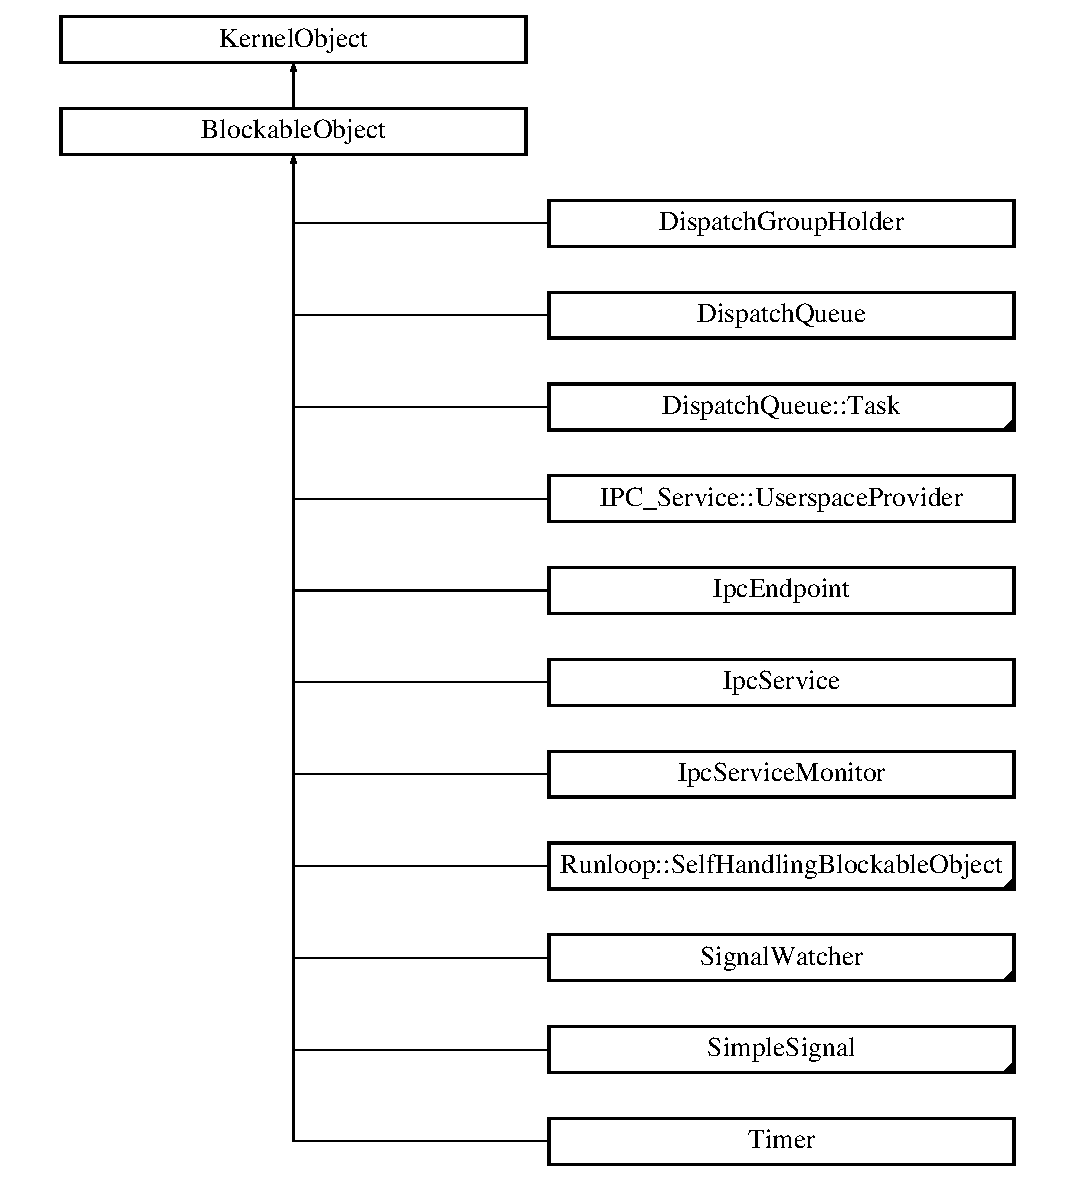
\includegraphics[height=12.000000cm]{class_blockable_object}
\end{center}
\end{figure}
\subsection*{Public Member Functions}
\begin{DoxyCompactItemize}
\item 
\mbox{\Hypertarget{class_blockable_object_a7fcae647f5c77522758c7b380556270a}\label{class_blockable_object_a7fcae647f5c77522758c7b380556270a}} 
const char $\ast$ {\bfseries Get\+Class\+Name} (U\+Int32 level)
\item 
\mbox{\Hypertarget{class_blockable_object_acc62e90014951c5bb0dc78e4d7007d74}\label{class_blockable_object_acc62e90014951c5bb0dc78e4d7007d74}} 
virtual void {\bfseries Register\+Observer} (\hyperlink{class_signal_watcher}{Signal\+Watcher} $\ast$watcher)
\item 
\mbox{\Hypertarget{class_blockable_object_a2e9cf7519914139866e17bbf10a74dfd}\label{class_blockable_object_a2e9cf7519914139866e17bbf10a74dfd}} 
virtual void {\bfseries Unregister\+Observer} (\hyperlink{class_signal_watcher}{Signal\+Watcher} $\ast$watcher)
\item 
\mbox{\Hypertarget{class_blockable_object_ae7010f91737c37796fcc5ad99f129265}\label{class_blockable_object_ae7010f91737c37796fcc5ad99f129265}} 
virtual bool {\bfseries Is\+Signalled} (void)
\item 
\mbox{\Hypertarget{class_blockable_object_afcfe6d01f5ecec42b390cb4d6a98d1ef}\label{class_blockable_object_afcfe6d01f5ecec42b390cb4d6a98d1ef}} 
virtual \hyperlink{class_kernel_array}{Kernel\+Array} $\ast$ {\bfseries Current\+Signals} (void)
\end{DoxyCompactItemize}
\subsection*{Static Public Member Functions}
\begin{DoxyCompactItemize}
\item 
\mbox{\Hypertarget{class_blockable_object_ad3abd46cd8e31a8691a1c564fcda83fc}\label{class_blockable_object_ad3abd46cd8e31a8691a1c564fcda83fc}} 
static void {\bfseries Configure\+Service} (void)
\end{DoxyCompactItemize}
\subsection*{Protected Member Functions}
\begin{DoxyCompactItemize}
\item 
\mbox{\Hypertarget{class_blockable_object_a6326633563601e0b22ef3d38c09c72fb}\label{class_blockable_object_a6326633563601e0b22ef3d38c09c72fb}} 
\hyperlink{class_kernel_array}{Kernel\+Array} $\ast$ {\bfseries This\+Current\+Signals} (void)
\item 
\mbox{\Hypertarget{class_blockable_object_a9b76187d71a80f78bad22e801fdd6317}\label{class_blockable_object_a9b76187d71a80f78bad22e801fdd6317}} 
virtual bool {\bfseries Check\+Signal} (void)
\item 
\mbox{\Hypertarget{class_blockable_object_a32fa6d1b6011a0b8bb9b651455b17df0}\label{class_blockable_object_a32fa6d1b6011a0b8bb9b651455b17df0}} 
void {\bfseries Set\+Signalled} (\hyperlink{class_blockable_object}{Blockable\+Object} $\ast$sender, bool active)
\end{DoxyCompactItemize}
\subsection*{Protected Attributes}
\begin{DoxyCompactItemize}
\item 
\mbox{\Hypertarget{class_blockable_object_a7a24c8b30ed53a5e34a81381cc9c98c0}\label{class_blockable_object_a7a24c8b30ed53a5e34a81381cc9c98c0}} 
\hyperlink{class_hardcore_spin_lock}{Hardcore\+Spin\+Lock} {\bfseries \+\_\+locker}
\end{DoxyCompactItemize}
\subsection*{Private Member Functions}
\begin{DoxyCompactItemize}
\item 
\mbox{\Hypertarget{class_blockable_object_ac05ea6392432f4d6bbae05fffb01f12a}\label{class_blockable_object_ac05ea6392432f4d6bbae05fffb01f12a}} 
void {\bfseries Do\+Signal} (bool active)
\end{DoxyCompactItemize}
\subsection*{Private Attributes}
\begin{DoxyCompactItemize}
\item 
\mbox{\Hypertarget{class_blockable_object_a5a4404223821f330f5f97cc0585ba7c3}\label{class_blockable_object_a5a4404223821f330f5f97cc0585ba7c3}} 
\hyperlink{class_kernel_array}{Kernel\+Array} $\ast$ {\bfseries \+\_\+watchers}
\item 
\mbox{\Hypertarget{class_blockable_object_ac8a9b85723f7ac7ef5fd690625ea69d2}\label{class_blockable_object_ac8a9b85723f7ac7ef5fd690625ea69d2}} 
\hyperlink{class_kernel_array}{Kernel\+Array} $\ast$ {\bfseries \+\_\+signals}
\item 
\mbox{\Hypertarget{class_blockable_object_a254bf323d64eb40d9608ad695d451208}\label{class_blockable_object_a254bf323d64eb40d9608ad695d451208}} 
bool {\bfseries \+\_\+self\+Signal}
\item 
\mbox{\Hypertarget{class_blockable_object_a6765b0109ed6a6db6c5e78998dbcb5eb}\label{class_blockable_object_a6765b0109ed6a6db6c5e78998dbcb5eb}} 
bool {\bfseries \+\_\+signalled}
\end{DoxyCompactItemize}


The documentation for this class was generated from the following files\+:\begin{DoxyCompactItemize}
\item 
Blocking.\+h\item 
Blocking.\+cpp\item 
Blocking\+\_\+\+Service.\+cpp\end{DoxyCompactItemize}

\hypertarget{class_cathode_ray_tube}{}\section{Cathode\+Ray\+Tube Class Reference}
\label{class_cathode_ray_tube}\index{Cathode\+Ray\+Tube@{Cathode\+Ray\+Tube}}
\subsection*{Public Member Functions}
\begin{DoxyCompactItemize}
\item 
\mbox{\Hypertarget{class_cathode_ray_tube_a1ee9fdda3c9182cc88969f882240239e}\label{class_cathode_ray_tube_a1ee9fdda3c9182cc88969f882240239e}} 
int {\bfseries Width} (void)
\item 
\mbox{\Hypertarget{class_cathode_ray_tube_add4a92d30872710612c7c6b145e1bd2e}\label{class_cathode_ray_tube_add4a92d30872710612c7c6b145e1bd2e}} 
int {\bfseries Height} (void)
\item 
\mbox{\Hypertarget{class_cathode_ray_tube_a8c635a7d588bdee1e89803bce01fb570}\label{class_cathode_ray_tube_a8c635a7d588bdee1e89803bce01fb570}} 
char $\ast$ {\bfseries Frame\+Buffer} (void)
\item 
\mbox{\Hypertarget{class_cathode_ray_tube_ac34d60890ce753329ef85511b88de24d}\label{class_cathode_ray_tube_ac34d60890ce753329ef85511b88de24d}} 
int {\bfseries Get\+Cursor\+Offset} (void)
\item 
\mbox{\Hypertarget{class_cathode_ray_tube_a98baf39ba4fecd2b2371a7b56e877346}\label{class_cathode_ray_tube_a98baf39ba4fecd2b2371a7b56e877346}} 
void {\bfseries Set\+Cursor\+Offset} (int offset)
\item 
\mbox{\Hypertarget{class_cathode_ray_tube_a03ab2f1fef56e75b52054ed9a23e876e}\label{class_cathode_ray_tube_a03ab2f1fef56e75b52054ed9a23e876e}} 
void {\bfseries Offset\+To\+Xy} (int offset, int $\ast$x, int $\ast$y)
\item 
\mbox{\Hypertarget{class_cathode_ray_tube_a9bb9750db449655a7489c4b60054ff81}\label{class_cathode_ray_tube_a9bb9750db449655a7489c4b60054ff81}} 
int {\bfseries Xy\+To\+Offset} (int x, int y)
\item 
\mbox{\Hypertarget{class_cathode_ray_tube_aa36a3798fafe70d85512d128b66b41ad}\label{class_cathode_ray_tube_aa36a3798fafe70d85512d128b66b41ad}} 
void {\bfseries Clear} (void)
\end{DoxyCompactItemize}
\subsection*{Private Attributes}
\begin{DoxyCompactItemize}
\item 
\mbox{\Hypertarget{class_cathode_ray_tube_a79c218fbba6ff113b25546c0ca856f73}\label{class_cathode_ray_tube_a79c218fbba6ff113b25546c0ca856f73}} 
bool {\bfseries set}
\item 
\mbox{\Hypertarget{class_cathode_ray_tube_a533c9335b714b27033b5a206b0b5949e}\label{class_cathode_ray_tube_a533c9335b714b27033b5a206b0b5949e}} 
int {\bfseries got}
\end{DoxyCompactItemize}


The documentation for this class was generated from the following file\+:\begin{DoxyCompactItemize}
\item 
debug.\+cpp\end{DoxyCompactItemize}

\hypertarget{class_internal_1_1_chunk}{}\section{Internal\+:\+:Chunk Class Reference}
\label{class_internal_1_1_chunk}\index{Internal\+::\+Chunk@{Internal\+::\+Chunk}}
Inheritance diagram for Internal\+:\+:Chunk\+:\begin{figure}[H]
\begin{center}
\leavevmode
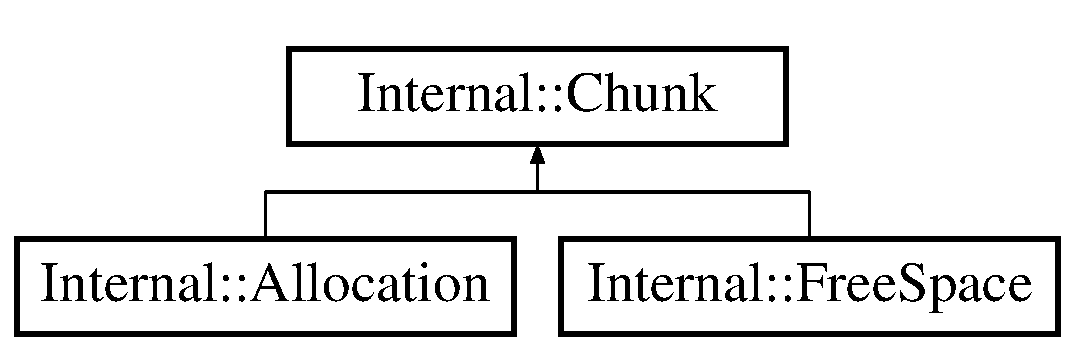
\includegraphics[height=2.000000cm]{class_internal_1_1_chunk}
\end{center}
\end{figure}
\subsection*{Public Types}
\begin{DoxyCompactItemize}
\item 
\mbox{\Hypertarget{class_internal_1_1_chunk_ab95e8afeb4d71a68331154ac5e318f7b}\label{class_internal_1_1_chunk_ab95e8afeb4d71a68331154ac5e318f7b}} 
enum {\bfseries Chunk\+Type} \{ {\bfseries Chunk\+Free}, 
{\bfseries Chunk\+Allocated}, 
{\bfseries Chunk\+End}
 \}
\end{DoxyCompactItemize}
\subsection*{Public Member Functions}
\begin{DoxyCompactItemize}
\item 
\mbox{\Hypertarget{class_internal_1_1_chunk_a72381e96bf7266774d4fe4999b2be009}\label{class_internal_1_1_chunk_a72381e96bf7266774d4fe4999b2be009}} 
{\bfseries Chunk} (Chunk\+Type new\+Type, Basic\+Heap\+::h\+\_\+size size)
\item 
\mbox{\Hypertarget{class_internal_1_1_chunk_a8b80771d7218ea6827d4872d3f9abab9}\label{class_internal_1_1_chunk_a8b80771d7218ea6827d4872d3f9abab9}} 
Chunk\+Type {\bfseries Type} (void)
\item 
\mbox{\Hypertarget{class_internal_1_1_chunk_ac053bf3bc4368a64903683a3f7ad2af9}\label{class_internal_1_1_chunk_ac053bf3bc4368a64903683a3f7ad2af9}} 
Basic\+Heap\+::h\+\_\+size {\bfseries Size} (void)
\item 
\mbox{\Hypertarget{class_internal_1_1_chunk_a8cc473a68b10da970ab3cab3ebfe9b97}\label{class_internal_1_1_chunk_a8cc473a68b10da970ab3cab3ebfe9b97}} 
\hyperlink{class_internal_1_1_chunk}{Chunk} $\ast$ {\bfseries Next} (void)
\end{DoxyCompactItemize}
\subsection*{Protected Attributes}
\begin{DoxyCompactItemize}
\item 
\mbox{\Hypertarget{class_internal_1_1_chunk_abc79836afba4e11ab3a9bcad0f8834b5}\label{class_internal_1_1_chunk_abc79836afba4e11ab3a9bcad0f8834b5}} 
Basic\+Heap\+::h\+\_\+size {\bfseries \+\_\+size}
\end{DoxyCompactItemize}
\subsection*{Private Attributes}
\begin{DoxyCompactItemize}
\item 
\mbox{\Hypertarget{class_internal_1_1_chunk_a2664fddcaeae17b93db51b0565e6df89}\label{class_internal_1_1_chunk_a2664fddcaeae17b93db51b0565e6df89}} 
Chunk\+Type {\bfseries \+\_\+type}
\end{DoxyCompactItemize}


The documentation for this class was generated from the following file\+:\begin{DoxyCompactItemize}
\item 
Basic\+Heap.\+cpp\end{DoxyCompactItemize}

\hypertarget{class_console_driver_1_1_colour}{}\section{Console\+Driver\+:\+:Colour Class Reference}
\label{class_console_driver_1_1_colour}\index{Console\+Driver\+::\+Colour@{Console\+Driver\+::\+Colour}}
\subsection*{Public Member Functions}
\begin{DoxyCompactItemize}
\item 
\mbox{\Hypertarget{class_console_driver_1_1_colour_a42162617488645335fac248ba5ef0e35}\label{class_console_driver_1_1_colour_a42162617488645335fac248ba5ef0e35}} 
{\bfseries Colour} (U\+Int8 r, U\+Int8 g, U\+Int8 b)
\end{DoxyCompactItemize}
\subsection*{Public Attributes}
\begin{DoxyCompactItemize}
\item 
\mbox{\Hypertarget{class_console_driver_1_1_colour_a25b20b8c051038a6af1b2a2875a13267}\label{class_console_driver_1_1_colour_a25b20b8c051038a6af1b2a2875a13267}} 
U\+Int8 {\bfseries red}
\item 
\mbox{\Hypertarget{class_console_driver_1_1_colour_aa2a37b5f06665216658a2499b802a7bc}\label{class_console_driver_1_1_colour_aa2a37b5f06665216658a2499b802a7bc}} 
U\+Int8 {\bfseries green}
\item 
\mbox{\Hypertarget{class_console_driver_1_1_colour_a18ed342c4ec7b1e27c9190ec72618e83}\label{class_console_driver_1_1_colour_a18ed342c4ec7b1e27c9190ec72618e83}} 
U\+Int8 {\bfseries blue}
\end{DoxyCompactItemize}


The documentation for this class was generated from the following file\+:\begin{DoxyCompactItemize}
\item 
Console.\+h\end{DoxyCompactItemize}

\hypertarget{class_standard_p_c___internal_1_1_p_s2_controller_1_1_command}{}\section{Standard\+P\+C\+\_\+\+Internal\+:\+:P\+S2\+Controller\+:\+:Command Class Reference}
\label{class_standard_p_c___internal_1_1_p_s2_controller_1_1_command}\index{Standard\+P\+C\+\_\+\+Internal\+::\+P\+S2\+Controller\+::\+Command@{Standard\+P\+C\+\_\+\+Internal\+::\+P\+S2\+Controller\+::\+Command}}
Inheritance diagram for Standard\+P\+C\+\_\+\+Internal\+:\+:P\+S2\+Controller\+:\+:Command\+:\begin{figure}[H]
\begin{center}
\leavevmode
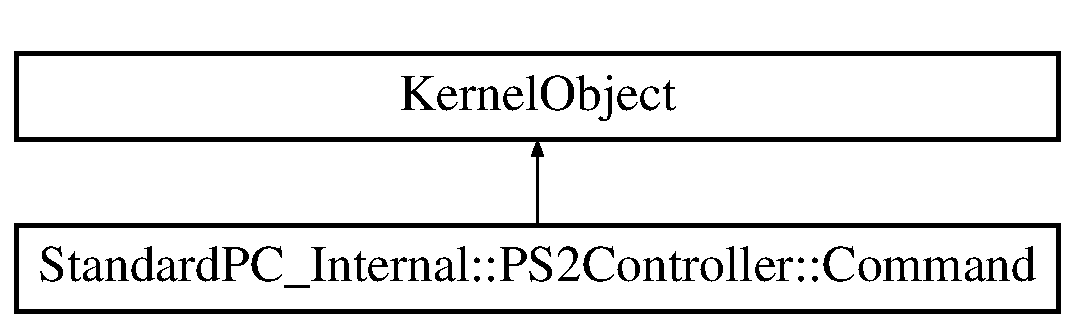
\includegraphics[height=2.000000cm]{class_standard_p_c___internal_1_1_p_s2_controller_1_1_command}
\end{center}
\end{figure}
\subsection*{Public Member Functions}
\begin{DoxyCompactItemize}
\item 
\mbox{\Hypertarget{class_standard_p_c___internal_1_1_p_s2_controller_1_1_command_a18271c7299d70aa610db684e733c8a31}\label{class_standard_p_c___internal_1_1_p_s2_controller_1_1_command_a18271c7299d70aa610db684e733c8a31}} 
{\bfseries Command} (\hyperlink{classbicycle_1_1function}{bicycle\+::function}$<$ void(void)$>$ send, \hyperlink{classbicycle_1_1function}{bicycle\+::function}$<$ void(U\+Int8 $\ast$)$>$ response, int expected)
\item 
\mbox{\Hypertarget{class_standard_p_c___internal_1_1_p_s2_controller_1_1_command_a42fd7dfa5ed34eb37cb2f9b0c45bc111}\label{class_standard_p_c___internal_1_1_p_s2_controller_1_1_command_a42fd7dfa5ed34eb37cb2f9b0c45bc111}} 
bool {\bfseries Run} (void)
\item 
\mbox{\Hypertarget{class_standard_p_c___internal_1_1_p_s2_controller_1_1_command_ab35156844379c7bdd154ca39535b11eb}\label{class_standard_p_c___internal_1_1_p_s2_controller_1_1_command_ab35156844379c7bdd154ca39535b11eb}} 
bool {\bfseries Add\+Byte} (U\+Int8 data)
\end{DoxyCompactItemize}
\subsection*{Private Attributes}
\begin{DoxyCompactItemize}
\item 
\mbox{\Hypertarget{class_standard_p_c___internal_1_1_p_s2_controller_1_1_command_ae9ea09a4f0b21dd90ce03f5ef31de5dc}\label{class_standard_p_c___internal_1_1_p_s2_controller_1_1_command_ae9ea09a4f0b21dd90ce03f5ef31de5dc}} 
\hyperlink{classbicycle_1_1function}{bicycle\+::function}$<$ void(void)$>$ {\bfseries \+\_\+send}
\item 
\mbox{\Hypertarget{class_standard_p_c___internal_1_1_p_s2_controller_1_1_command_af0191786a5119b3ebc2ae7294d07d285}\label{class_standard_p_c___internal_1_1_p_s2_controller_1_1_command_af0191786a5119b3ebc2ae7294d07d285}} 
\hyperlink{classbicycle_1_1function}{bicycle\+::function}$<$ void(U\+Int8 $\ast$)$>$ {\bfseries \+\_\+response}
\item 
\mbox{\Hypertarget{class_standard_p_c___internal_1_1_p_s2_controller_1_1_command_aae34086a4164bf871a11adb7b992ba5a}\label{class_standard_p_c___internal_1_1_p_s2_controller_1_1_command_aae34086a4164bf871a11adb7b992ba5a}} 
U\+Int8 {\bfseries \+\_\+buf} \mbox{[}10\mbox{]}
\item 
\mbox{\Hypertarget{class_standard_p_c___internal_1_1_p_s2_controller_1_1_command_a7427d625cc5e4dafead570ffc5d50b6a}\label{class_standard_p_c___internal_1_1_p_s2_controller_1_1_command_a7427d625cc5e4dafead570ffc5d50b6a}} 
int {\bfseries \+\_\+buf\+Size}
\item 
\mbox{\Hypertarget{class_standard_p_c___internal_1_1_p_s2_controller_1_1_command_a878b30ece9502bea3c2e7453dcc54672}\label{class_standard_p_c___internal_1_1_p_s2_controller_1_1_command_a878b30ece9502bea3c2e7453dcc54672}} 
int {\bfseries \+\_\+buf\+Need}
\end{DoxyCompactItemize}
\subsection*{Additional Inherited Members}


The documentation for this class was generated from the following file\+:\begin{DoxyCompactItemize}
\item 
Standard\+P\+C.\+cpp\end{DoxyCompactItemize}

\hypertarget{classbicycle_1_1concrete__function}{}\section{bicycle\+:\+:concrete\+\_\+function$<$ Func, Result, Args $>$ Class Template Reference}
\label{classbicycle_1_1concrete__function}\index{bicycle\+::concrete\+\_\+function$<$ Func, Result, Args $>$@{bicycle\+::concrete\+\_\+function$<$ Func, Result, Args $>$}}
Inheritance diagram for bicycle\+:\+:concrete\+\_\+function$<$ Func, Result, Args $>$\+:\begin{figure}[H]
\begin{center}
\leavevmode
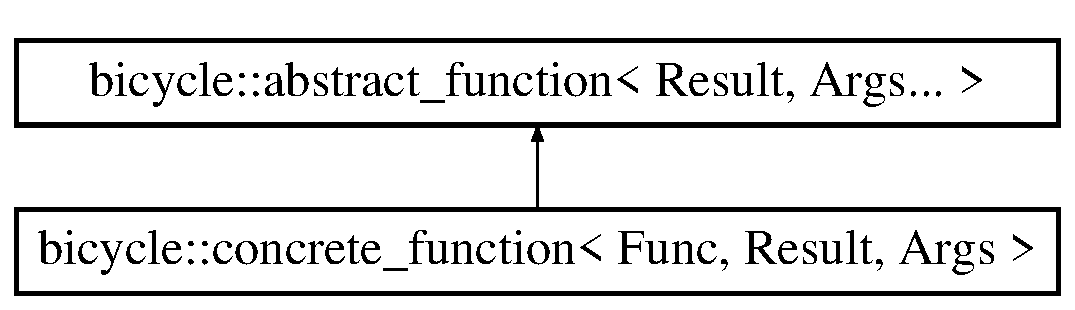
\includegraphics[height=2.000000cm]{classbicycle_1_1concrete__function}
\end{center}
\end{figure}
\subsection*{Public Member Functions}
\begin{DoxyCompactItemize}
\item 
\mbox{\Hypertarget{classbicycle_1_1concrete__function_af923ccdf1171fa1fdb6d72c5658ef90e}\label{classbicycle_1_1concrete__function_af923ccdf1171fa1fdb6d72c5658ef90e}} 
{\bfseries concrete\+\_\+function} (const Func \&x)
\item 
\mbox{\Hypertarget{classbicycle_1_1concrete__function_ae06f11989f73271f6151e1095c2abb02}\label{classbicycle_1_1concrete__function_ae06f11989f73271f6151e1095c2abb02}} 
Result {\bfseries operator()} (Args... args) override
\item 
\mbox{\Hypertarget{classbicycle_1_1concrete__function_a784c42fdba4d6970e2f2a40cd064a26e}\label{classbicycle_1_1concrete__function_a784c42fdba4d6970e2f2a40cd064a26e}} 
\hyperlink{classbicycle_1_1concrete__function}{concrete\+\_\+function} $\ast$ {\bfseries clone} () const override
\end{DoxyCompactItemize}
\subsection*{Private Attributes}
\begin{DoxyCompactItemize}
\item 
\mbox{\Hypertarget{classbicycle_1_1concrete__function_a9f0465bca48b1800f2fafafed2473c61}\label{classbicycle_1_1concrete__function_a9f0465bca48b1800f2fafafed2473c61}} 
Func {\bfseries f}
\end{DoxyCompactItemize}


The documentation for this class was generated from the following file\+:\begin{DoxyCompactItemize}
\item 
Kernel\+Function.\+h\end{DoxyCompactItemize}

\hypertarget{class_configure_a_t_a}{}\section{Configure\+A\+TA Class Reference}
\label{class_configure_a_t_a}\index{Configure\+A\+TA@{Configure\+A\+TA}}
Inheritance diagram for Configure\+A\+TA\+:\begin{figure}[H]
\begin{center}
\leavevmode
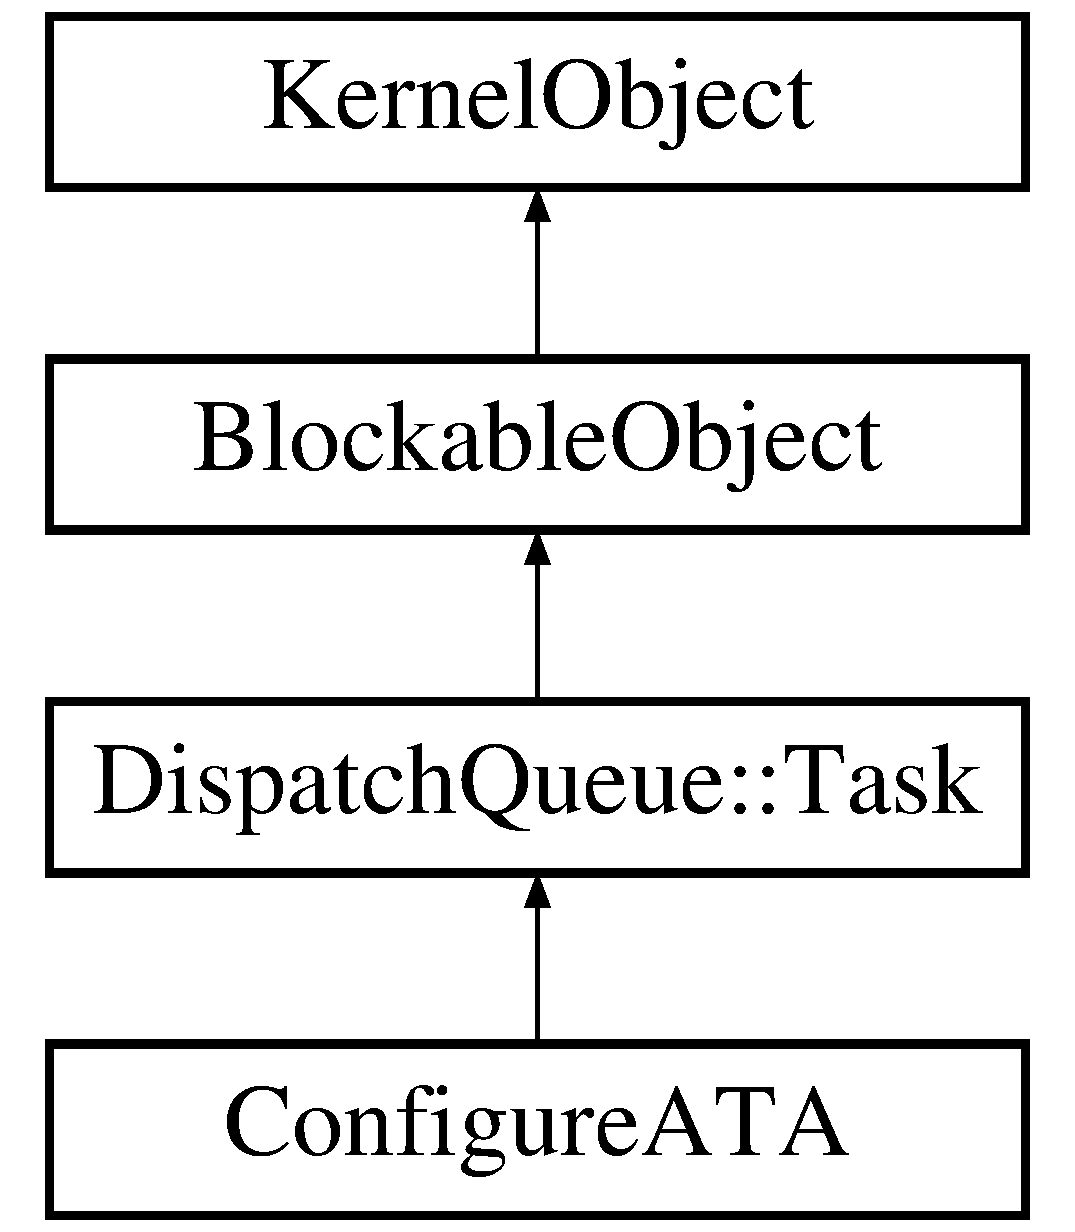
\includegraphics[height=4.000000cm]{class_configure_a_t_a}
\end{center}
\end{figure}
\subsection*{Public Member Functions}
\begin{DoxyCompactItemize}
\item 
\mbox{\Hypertarget{class_configure_a_t_a_a6adf1b2ad320729ae84f851adbbf4c09}\label{class_configure_a_t_a_a6adf1b2ad320729ae84f851adbbf4c09}} 
const char $\ast$ {\bfseries Get\+Class\+Name} (U\+Int32 level)
\item 
\mbox{\Hypertarget{class_configure_a_t_a_ae6f2afeaabb8b4edf19ce009f8e61c59}\label{class_configure_a_t_a_ae6f2afeaabb8b4edf19ce009f8e61c59}} 
{\bfseries Configure\+A\+TA} (\hyperlink{class_a_t_a_driver}{A\+T\+A\+Driver} $\ast$driver, bool use\+D\+MA)
\end{DoxyCompactItemize}
\subsection*{Protected Member Functions}
\begin{DoxyCompactItemize}
\item 
\mbox{\Hypertarget{class_configure_a_t_a_a40c16425cfde67d09deb7a7fa06ebee2}\label{class_configure_a_t_a_a40c16425cfde67d09deb7a7fa06ebee2}} 
void {\bfseries Execute} (void)
\end{DoxyCompactItemize}
\subsection*{Private Attributes}
\begin{DoxyCompactItemize}
\item 
\mbox{\Hypertarget{class_configure_a_t_a_a466e12e38b33d00f97b5c485ce54ab57}\label{class_configure_a_t_a_a466e12e38b33d00f97b5c485ce54ab57}} 
\hyperlink{class_a_t_a_driver}{A\+T\+A\+Driver} $\ast$ {\bfseries \+\_\+owner}
\item 
\mbox{\Hypertarget{class_configure_a_t_a_ad6faca95744b0d5a47a4df5ceef4f5a7}\label{class_configure_a_t_a_ad6faca95744b0d5a47a4df5ceef4f5a7}} 
bool {\bfseries \+\_\+use\+D\+MA}
\end{DoxyCompactItemize}
\subsection*{Additional Inherited Members}


The documentation for this class was generated from the following file\+:\begin{DoxyCompactItemize}
\item 
Driver\+\_\+\+A\+T\+A.\+cpp\end{DoxyCompactItemize}

\hypertarget{class_generic_provider_1_1_connection}{}\section{Generic\+Provider\+:\+:Connection Class Reference}
\label{class_generic_provider_1_1_connection}\index{Generic\+Provider\+::\+Connection@{Generic\+Provider\+::\+Connection}}
Inheritance diagram for Generic\+Provider\+:\+:Connection\+:\begin{figure}[H]
\begin{center}
\leavevmode
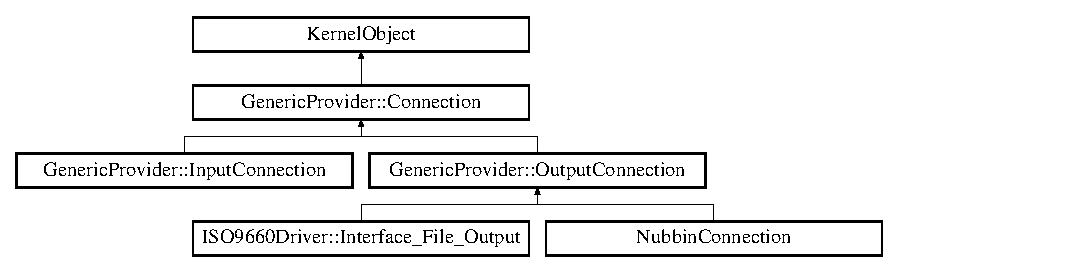
\includegraphics[height=3.204578cm]{class_generic_provider_1_1_connection}
\end{center}
\end{figure}
\subsection*{Public Member Functions}
\begin{DoxyCompactItemize}
\item 
\mbox{\Hypertarget{class_generic_provider_1_1_connection_a1a0e4585cc68a03139b7b6f90018c953}\label{class_generic_provider_1_1_connection_a1a0e4585cc68a03139b7b6f90018c953}} 
const char $\ast$ {\bfseries Get\+Class\+Name} (U\+Int32 level)
\item 
\mbox{\Hypertarget{class_generic_provider_1_1_connection_a2ca2ef660ec08ebd09e76adef06ec256}\label{class_generic_provider_1_1_connection_a2ca2ef660ec08ebd09e76adef06ec256}} 
\hyperlink{class_ipc_endpoint}{Ipc\+Endpoint} $\ast$ {\bfseries Link} (void)
\end{DoxyCompactItemize}
\subsection*{Protected Member Functions}
\begin{DoxyCompactItemize}
\item 
\mbox{\Hypertarget{class_generic_provider_1_1_connection_a7cb415aad20366a5efea335764305d2c}\label{class_generic_provider_1_1_connection_a7cb415aad20366a5efea335764305d2c}} 
{\bfseries Connection} (\hyperlink{class_generic_provider}{Generic\+Provider} $\ast$owner, \hyperlink{class_ipc_endpoint}{Ipc\+Endpoint} $\ast$connection)
\end{DoxyCompactItemize}
\subsection*{Private Attributes}
\begin{DoxyCompactItemize}
\item 
\mbox{\Hypertarget{class_generic_provider_1_1_connection_a277c17f0e1003a10867f5ceab3774acf}\label{class_generic_provider_1_1_connection_a277c17f0e1003a10867f5ceab3774acf}} 
\hyperlink{class_generic_provider}{Generic\+Provider} $\ast$ {\bfseries \+\_\+owner}
\item 
\mbox{\Hypertarget{class_generic_provider_1_1_connection_a46d806055858dce259f81d6a9d425a22}\label{class_generic_provider_1_1_connection_a46d806055858dce259f81d6a9d425a22}} 
\hyperlink{class_ipc_endpoint}{Ipc\+Endpoint} $\ast$ {\bfseries \+\_\+connection}
\end{DoxyCompactItemize}
\subsection*{Additional Inherited Members}


The documentation for this class was generated from the following files\+:\begin{DoxyCompactItemize}
\item 
Provider.\+h\item 
Provider.\+cpp\end{DoxyCompactItemize}

\hypertarget{class_provider_driver_1_1_connection}{}\section{Provider\+Driver\+:\+:Connection Class Reference}
\label{class_provider_driver_1_1_connection}\index{Provider\+Driver\+::\+Connection@{Provider\+Driver\+::\+Connection}}
Inheritance diagram for Provider\+Driver\+:\+:Connection\+:\begin{figure}[H]
\begin{center}
\leavevmode
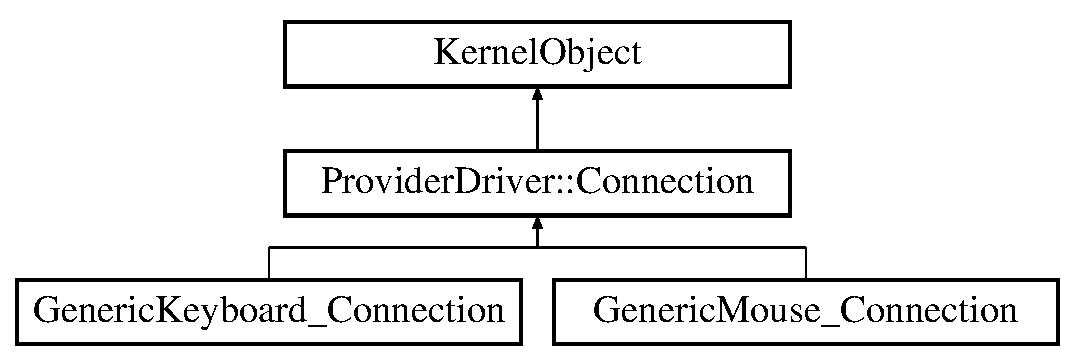
\includegraphics[height=3.000000cm]{class_provider_driver_1_1_connection}
\end{center}
\end{figure}
\subsection*{Public Member Functions}
\begin{DoxyCompactItemize}
\item 
\mbox{\Hypertarget{class_provider_driver_1_1_connection_aaf69c031c359e050378627914d1b1645}\label{class_provider_driver_1_1_connection_aaf69c031c359e050378627914d1b1645}} 
{\bfseries Connection} (\hyperlink{class_provider_driver}{Provider\+Driver} $\ast$owner, \hyperlink{class_provider_driver_1_1_service}{Service} $\ast$service, \hyperlink{class_ipc_endpoint}{Ipc\+Endpoint} $\ast$connection)
\item 
\mbox{\Hypertarget{class_provider_driver_1_1_connection_ab96165eb11d8db20fd451a4066c74a61}\label{class_provider_driver_1_1_connection_ab96165eb11d8db20fd451a4066c74a61}} 
const char $\ast$ {\bfseries Get\+Class\+Name} (U\+Int32 level)
\item 
\mbox{\Hypertarget{class_provider_driver_1_1_connection_ab7f1baf6d5bc27b7c35c531f2d917cd9}\label{class_provider_driver_1_1_connection_ab7f1baf6d5bc27b7c35c531f2d917cd9}} 
\hyperlink{class_provider_driver_1_1_service}{Service} $\ast$ {\bfseries Base\+Service} (void)
\item 
\mbox{\Hypertarget{class_provider_driver_1_1_connection_a467446433448a38cea19a8387588610f}\label{class_provider_driver_1_1_connection_a467446433448a38cea19a8387588610f}} 
\hyperlink{class_ipc_endpoint}{Ipc\+Endpoint} $\ast$ {\bfseries Link} (void)
\end{DoxyCompactItemize}
\subsection*{Public Attributes}
\begin{DoxyCompactItemize}
\item 
\mbox{\Hypertarget{class_provider_driver_1_1_connection_a99ebed66c13be4560c6eca07108412a4}\label{class_provider_driver_1_1_connection_a99ebed66c13be4560c6eca07108412a4}} 
\hyperlink{classbicycle_1_1function}{bicycle\+::function}$<$ void(\hyperlink{class_kernel_buffer_memory}{Kernel\+Buffer\+Memory} $\ast$)$>$ {\bfseries message}
\item 
\mbox{\Hypertarget{class_provider_driver_1_1_connection_aecce7d06f85d0060c723197f85d2e180}\label{class_provider_driver_1_1_connection_aecce7d06f85d0060c723197f85d2e180}} 
\hyperlink{classbicycle_1_1function}{bicycle\+::function}$<$ void(void)$>$ {\bfseries stop}
\end{DoxyCompactItemize}
\subsection*{Private Attributes}
\begin{DoxyCompactItemize}
\item 
\mbox{\Hypertarget{class_provider_driver_1_1_connection_add255e527f1cb37b302423b6e556d705}\label{class_provider_driver_1_1_connection_add255e527f1cb37b302423b6e556d705}} 
\hyperlink{class_provider_driver}{Provider\+Driver} $\ast$ {\bfseries \+\_\+owner}
\item 
\mbox{\Hypertarget{class_provider_driver_1_1_connection_a224a560b89116fbc0cbb2826661cf3ec}\label{class_provider_driver_1_1_connection_a224a560b89116fbc0cbb2826661cf3ec}} 
\hyperlink{class_provider_driver_1_1_service}{Service} $\ast$ {\bfseries \+\_\+service}
\item 
\mbox{\Hypertarget{class_provider_driver_1_1_connection_a79a4c9628398e966468908fa6914bd53}\label{class_provider_driver_1_1_connection_a79a4c9628398e966468908fa6914bd53}} 
\hyperlink{class_ipc_endpoint}{Ipc\+Endpoint} $\ast$ {\bfseries \+\_\+connection}
\end{DoxyCompactItemize}
\subsection*{Additional Inherited Members}


The documentation for this class was generated from the following files\+:\begin{DoxyCompactItemize}
\item 
Driver.\+h\item 
Driver.\+cpp\end{DoxyCompactItemize}

\hypertarget{class_a_t_a_driver_drive_1_1_connection_handler}{}\section{A\+T\+A\+Driver\+Drive\+:\+:Connection\+Handler Class Reference}
\label{class_a_t_a_driver_drive_1_1_connection_handler}\index{A\+T\+A\+Driver\+Drive\+::\+Connection\+Handler@{A\+T\+A\+Driver\+Drive\+::\+Connection\+Handler}}
Inheritance diagram for A\+T\+A\+Driver\+Drive\+:\+:Connection\+Handler\+:\begin{figure}[H]
\begin{center}
\leavevmode
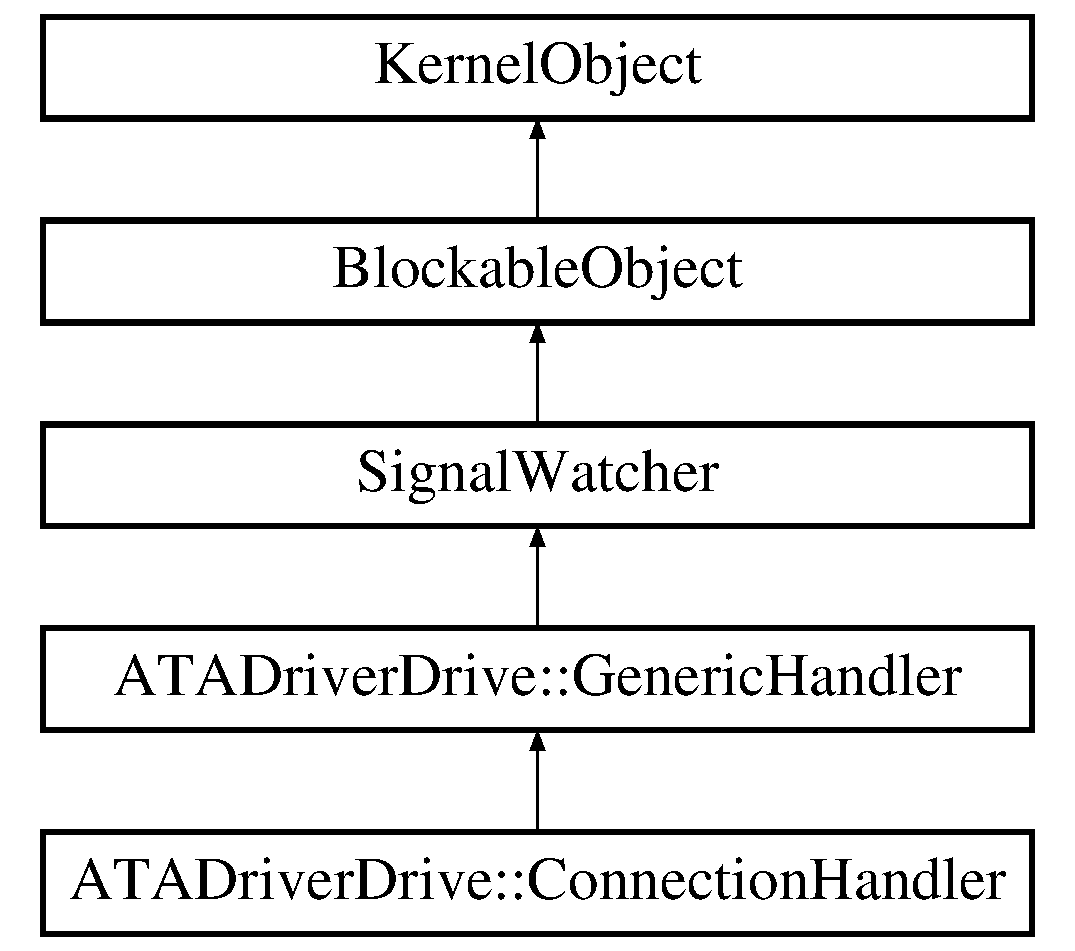
\includegraphics[height=5.000000cm]{class_a_t_a_driver_drive_1_1_connection_handler}
\end{center}
\end{figure}
\subsection*{Public Member Functions}
\begin{DoxyCompactItemize}
\item 
\mbox{\Hypertarget{class_a_t_a_driver_drive_1_1_connection_handler_add4de1606eee6dfb3bf70f21aa97bc52}\label{class_a_t_a_driver_drive_1_1_connection_handler_add4de1606eee6dfb3bf70f21aa97bc52}} 
const char $\ast$ {\bfseries Get\+Class\+Name} (U\+Int32 level)
\item 
\mbox{\Hypertarget{class_a_t_a_driver_drive_1_1_connection_handler_a2607b94166f4b8771d2206aaff8be7f0}\label{class_a_t_a_driver_drive_1_1_connection_handler_a2607b94166f4b8771d2206aaff8be7f0}} 
{\bfseries Connection\+Handler} (\hyperlink{class_a_t_a_driver_drive}{A\+T\+A\+Driver\+Drive} $\ast$owner)
\item 
\mbox{\Hypertarget{class_a_t_a_driver_drive_1_1_connection_handler_a3be6e60ed10d56d85de958e9374871d4}\label{class_a_t_a_driver_drive_1_1_connection_handler_a3be6e60ed10d56d85de958e9374871d4}} 
void {\bfseries Signal\+Changed} (\hyperlink{class_blockable_object}{Blockable\+Object} $\ast$watching, bool active)
\end{DoxyCompactItemize}
\subsection*{Additional Inherited Members}


The documentation for this class was generated from the following file\+:\begin{DoxyCompactItemize}
\item 
Driver\+\_\+\+A\+T\+A.\+cpp\end{DoxyCompactItemize}

\hypertarget{class_console_driver}{}\section{Console\+Driver Class Reference}
\label{class_console_driver}\index{Console\+Driver@{Console\+Driver}}
Inheritance diagram for Console\+Driver\+:\begin{figure}[H]
\begin{center}
\leavevmode
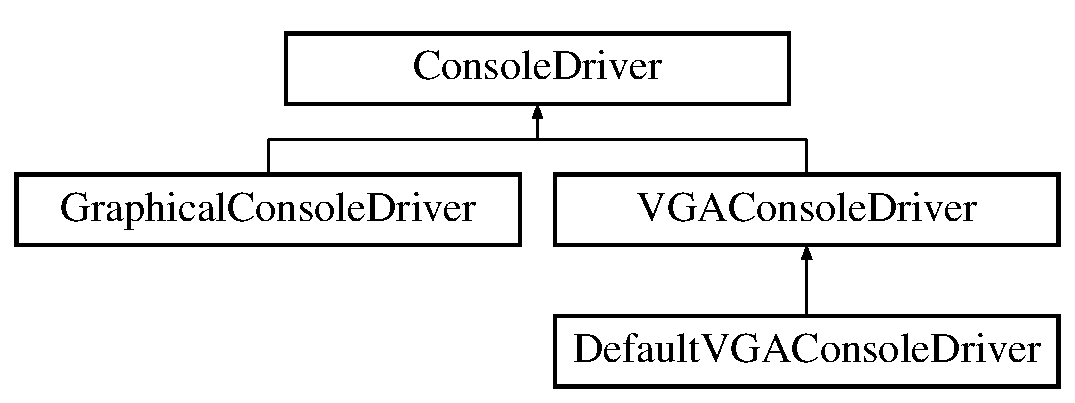
\includegraphics[height=3.000000cm]{class_console_driver}
\end{center}
\end{figure}
\subsection*{Classes}
\begin{DoxyCompactItemize}
\item 
class \hyperlink{class_console_driver_1_1_colour}{Colour}
\end{DoxyCompactItemize}
\subsection*{Public Member Functions}
\begin{DoxyCompactItemize}
\item 
\mbox{\Hypertarget{class_console_driver_ae382db5f8a03cd3eb6640668c94189c5}\label{class_console_driver_ae382db5f8a03cd3eb6640668c94189c5}} 
virtual void {\bfseries Set} (char c, int x, int y, \hyperlink{class_console_driver_1_1_colour}{Colour} foreground=\hyperlink{class_console_driver_1_1_colour}{Colour}(255, 255, 255), \hyperlink{class_console_driver_1_1_colour}{Colour} background=\hyperlink{class_console_driver_1_1_colour}{Colour}(0, 0, 0))=0
\item 
\mbox{\Hypertarget{class_console_driver_a5916d27374f57f5863a6ab5792b24ad6}\label{class_console_driver_a5916d27374f57f5863a6ab5792b24ad6}} 
virtual void {\bfseries Set\+Cursor} (int x, int y)=0
\item 
\mbox{\Hypertarget{class_console_driver_a0aefc44f4a7229bfe97be086730d8fbe}\label{class_console_driver_a0aefc44f4a7229bfe97be086730d8fbe}} 
virtual void {\bfseries Get\+Cursor} (int $\ast$x, int $\ast$y)=0
\item 
\mbox{\Hypertarget{class_console_driver_a09b75ec7e0714377eac28956d51e0eae}\label{class_console_driver_a09b75ec7e0714377eac28956d51e0eae}} 
virtual void {\bfseries Set\+Cursor\+Enabled} (bool enabled)=0
\item 
\mbox{\Hypertarget{class_console_driver_a2b801652c81112e4d2bc97f448f50166}\label{class_console_driver_a2b801652c81112e4d2bc97f448f50166}} 
virtual int {\bfseries Width} (void)=0
\item 
\mbox{\Hypertarget{class_console_driver_a010fedf93a07c9580a9d37fdb140536c}\label{class_console_driver_a010fedf93a07c9580a9d37fdb140536c}} 
virtual int {\bfseries Height} (void)=0
\item 
\mbox{\Hypertarget{class_console_driver_ac2cfde067e13c06d4e6b4abcc90357a1}\label{class_console_driver_ac2cfde067e13c06d4e6b4abcc90357a1}} 
virtual void {\bfseries Clear} (int x, int y, int w, int h)=0
\item 
\mbox{\Hypertarget{class_console_driver_a9d800bcf721d58b1c536bf99b7abc40e}\label{class_console_driver_a9d800bcf721d58b1c536bf99b7abc40e}} 
virtual void {\bfseries Copy} (int x\+From, int y\+From, int x\+To, int y\+To, int w, int h)=0
\end{DoxyCompactItemize}


The documentation for this class was generated from the following file\+:\begin{DoxyCompactItemize}
\item 
Console.\+h\end{DoxyCompactItemize}

\hypertarget{class_c_p_u_1_1_context}{}\section{C\+PU\+:\+:Context Class Reference}
\label{class_c_p_u_1_1_context}\index{C\+P\+U\+::\+Context@{C\+P\+U\+::\+Context}}
\subsection*{Public Member Functions}
\begin{DoxyCompactItemize}
\item 
\mbox{\Hypertarget{class_c_p_u_1_1_context_a1eb39f75ff9c4b407f184856ebfea95f}\label{class_c_p_u_1_1_context_a1eb39f75ff9c4b407f184856ebfea95f}} 
void {\bfseries Switch\+From} (\hyperlink{class_c_p_u_1_1_context}{Context} $\ast$$\ast$old\+Context)
\end{DoxyCompactItemize}
\subsection*{Public Attributes}
\begin{DoxyCompactItemize}
\item 
\mbox{\Hypertarget{class_c_p_u_1_1_context_a847a35a0d7e4387990dd68b83b358a17}\label{class_c_p_u_1_1_context_a847a35a0d7e4387990dd68b83b358a17}} 
U\+Int32 {\bfseries E\+DI}
\item 
\mbox{\Hypertarget{class_c_p_u_1_1_context_a8d5c58ab23deaae070bd2021ebcc98b4}\label{class_c_p_u_1_1_context_a8d5c58ab23deaae070bd2021ebcc98b4}} 
U\+Int32 {\bfseries E\+SI}
\item 
\mbox{\Hypertarget{class_c_p_u_1_1_context_acd814048ec2badce7560895f1b914ab0}\label{class_c_p_u_1_1_context_acd814048ec2badce7560895f1b914ab0}} 
U\+Int32 {\bfseries E\+BX}
\item 
\mbox{\Hypertarget{class_c_p_u_1_1_context_a16c8fa29ff62dad9337ba34afd02bec1}\label{class_c_p_u_1_1_context_a16c8fa29ff62dad9337ba34afd02bec1}} 
U\+Int32 {\bfseries E\+BP}
\item 
\mbox{\Hypertarget{class_c_p_u_1_1_context_aa41a3763abc75e81562b96a5e9d1907a}\label{class_c_p_u_1_1_context_aa41a3763abc75e81562b96a5e9d1907a}} 
U\+Int32 {\bfseries E\+IP}
\end{DoxyCompactItemize}


The documentation for this class was generated from the following files\+:\begin{DoxyCompactItemize}
\item 
C\+P\+U.\+h\item 
C\+P\+U.\+cpp\end{DoxyCompactItemize}

\hypertarget{class_standard_p_c_1_1_context_switching}{}\section{Standard\+PC\+:\+:Context\+Switching Class Reference}
\label{class_standard_p_c_1_1_context_switching}\index{Standard\+P\+C\+::\+Context\+Switching@{Standard\+P\+C\+::\+Context\+Switching}}
\subsection*{Static Public Member Functions}
\begin{DoxyCompactItemize}
\item 
\mbox{\Hypertarget{class_standard_p_c_1_1_context_switching_a916007a6599959c46cac1e126fdd7a32}\label{class_standard_p_c_1_1_context_switching_a916007a6599959c46cac1e126fdd7a32}} 
static void {\bfseries Initialise} (void)
\item 
\mbox{\Hypertarget{class_standard_p_c_1_1_context_switching_a9840f6fcfa04c78a1bd71e9a4ebd0e39}\label{class_standard_p_c_1_1_context_switching_a9840f6fcfa04c78a1bd71e9a4ebd0e39}} 
static void {\bfseries Entering\+Thread} (\hyperlink{class_thread}{Thread} $\ast$thread)
\item 
\mbox{\Hypertarget{class_standard_p_c_1_1_context_switching_a20e90a2068057fd8af6cddbbd6420577}\label{class_standard_p_c_1_1_context_switching_a20e90a2068057fd8af6cddbbd6420577}} 
static void {\bfseries Exiting\+Thread} (\hyperlink{class_thread}{Thread} $\ast$thread)
\end{DoxyCompactItemize}


The documentation for this class was generated from the following files\+:\begin{DoxyCompactItemize}
\item 
Standard\+P\+C.\+h\item 
Standard\+P\+C.\+cpp\end{DoxyCompactItemize}

\hypertarget{class_p_c_i_1_1_controller}{}\section{P\+CI\+:\+:Controller Class Reference}
\label{class_p_c_i_1_1_controller}\index{P\+C\+I\+::\+Controller@{P\+C\+I\+::\+Controller}}
Inheritance diagram for P\+CI\+:\+:Controller\+:\begin{figure}[H]
\begin{center}
\leavevmode
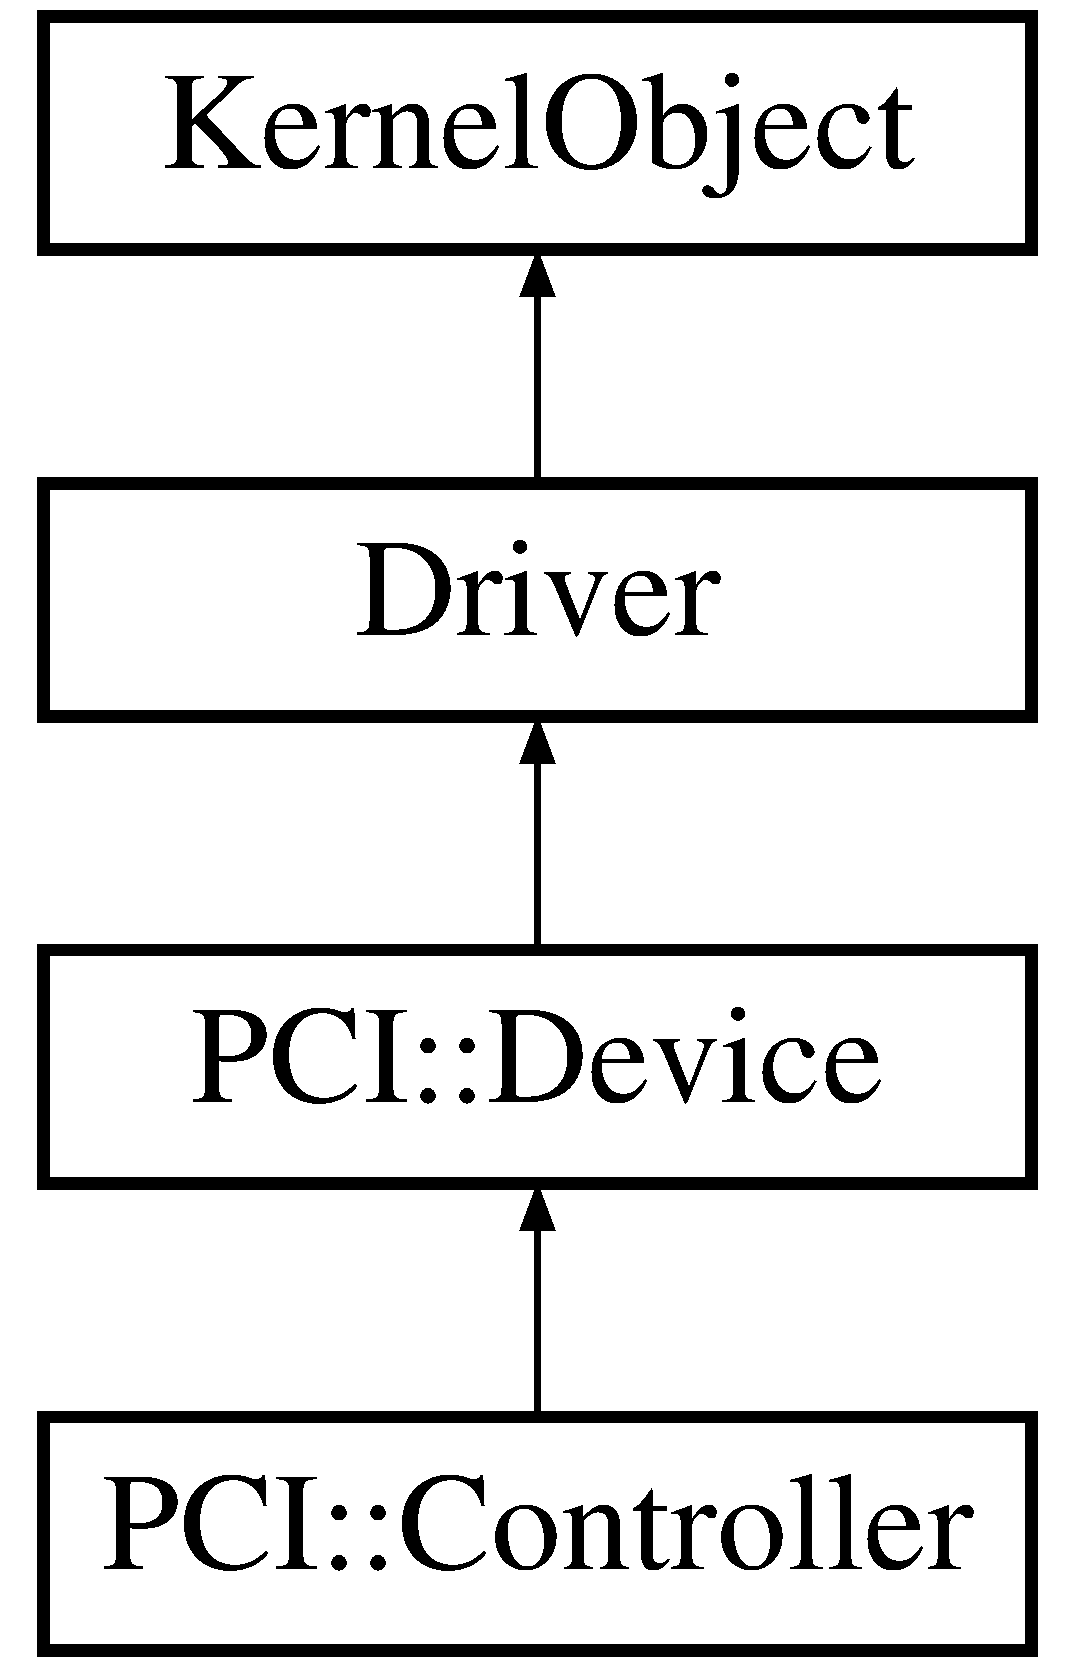
\includegraphics[height=4.000000cm]{class_p_c_i_1_1_controller}
\end{center}
\end{figure}
\subsection*{Public Member Functions}
\begin{DoxyCompactItemize}
\item 
\mbox{\Hypertarget{class_p_c_i_1_1_controller_a133af638b6cc15a6315301513e630b5e}\label{class_p_c_i_1_1_controller_a133af638b6cc15a6315301513e630b5e}} 
const char $\ast$ {\bfseries Get\+Class\+Name} (U\+Int32 level)
\item 
\mbox{\Hypertarget{class_p_c_i_1_1_controller_ab0998cb0f4ed2cf295a9d386eb66d0ea}\label{class_p_c_i_1_1_controller_ab0998cb0f4ed2cf295a9d386eb66d0ea}} 
{\bfseries Controller} (const char $\ast$name, U\+Int8 bus)
\item 
\mbox{\Hypertarget{class_p_c_i_1_1_controller_a82cf80c754e99e4b0c5355957d106678}\label{class_p_c_i_1_1_controller_a82cf80c754e99e4b0c5355957d106678}} 
void {\bfseries Check\+Function} (U\+Int8 device, U\+Int8 function)
\item 
\mbox{\Hypertarget{class_p_c_i_1_1_controller_a68d664ef4a7742d1b87d9364147775ca}\label{class_p_c_i_1_1_controller_a68d664ef4a7742d1b87d9364147775ca}} 
void {\bfseries Check\+Device} (U\+Int8 device)
\item 
\mbox{\Hypertarget{class_p_c_i_1_1_controller_a34391006bc15867b4e76ba1c8bb8bc23}\label{class_p_c_i_1_1_controller_a34391006bc15867b4e76ba1c8bb8bc23}} 
bool {\bfseries Start} (\hyperlink{class_driver}{Driver} $\ast$parent)
\end{DoxyCompactItemize}
\subsection*{Additional Inherited Members}


The documentation for this class was generated from the following file\+:\begin{DoxyCompactItemize}
\item 
pci.\+cpp\end{DoxyCompactItemize}

\hypertarget{class_convenient_sink}{}\section{Convenient\+Sink Class Reference}
\label{class_convenient_sink}\index{Convenient\+Sink@{Convenient\+Sink}}
Inheritance diagram for Convenient\+Sink\+:\begin{figure}[H]
\begin{center}
\leavevmode
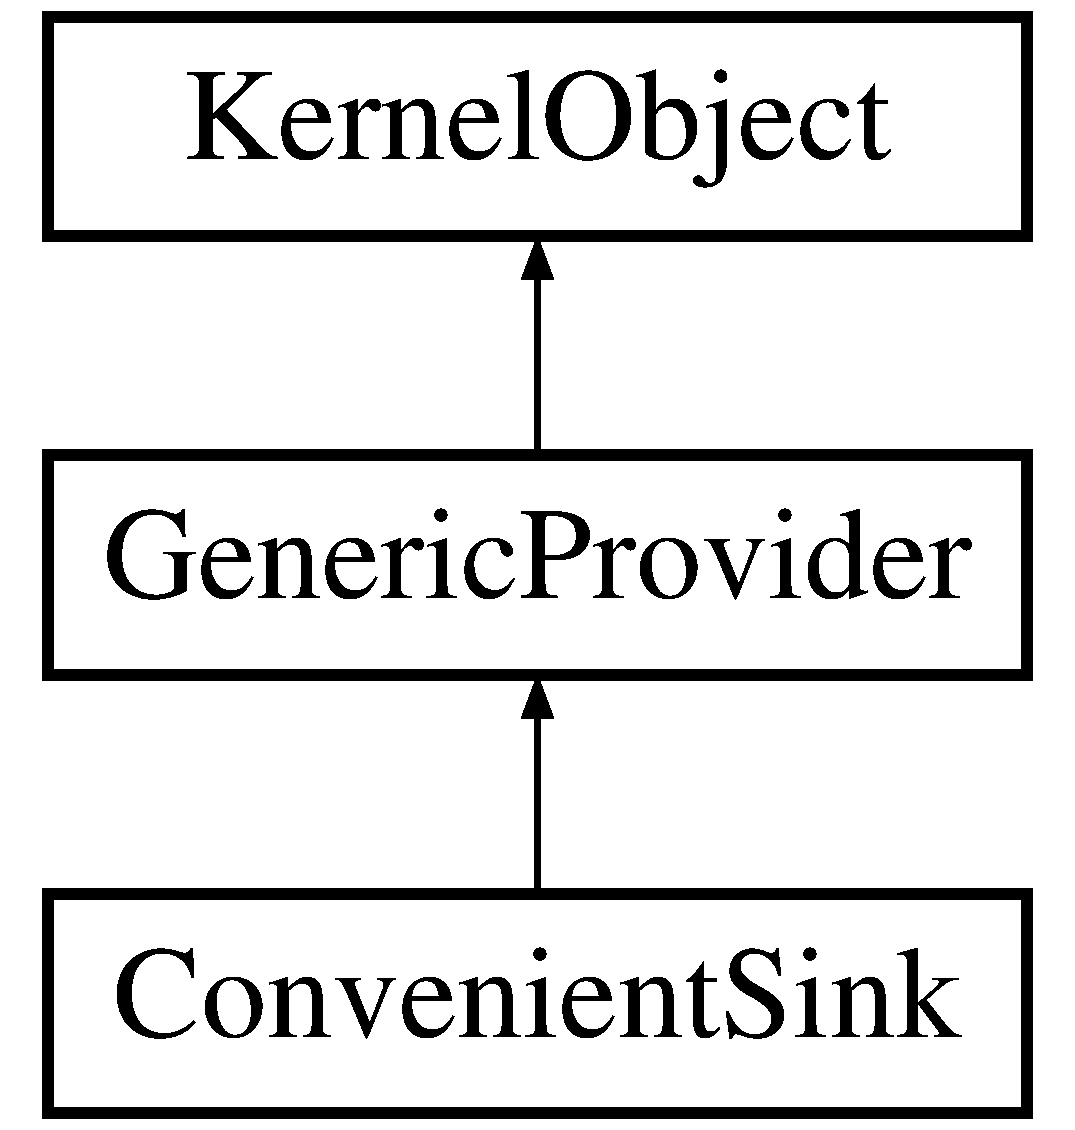
\includegraphics[height=3.000000cm]{class_convenient_sink}
\end{center}
\end{figure}
\subsection*{Public Member Functions}
\begin{DoxyCompactItemize}
\item 
\mbox{\Hypertarget{class_convenient_sink_a5de85f0a250db250ec8dbc13a8a4df1f}\label{class_convenient_sink_a5de85f0a250db250ec8dbc13a8a4df1f}} 
const char $\ast$ {\bfseries Get\+Class\+Name} (U\+Int32 level)
\item 
\mbox{\Hypertarget{class_convenient_sink_ad002c843d001c4e20b88be15326e94cf}\label{class_convenient_sink_ad002c843d001c4e20b88be15326e94cf}} 
{\bfseries Convenient\+Sink} (\hyperlink{class_runloop_thread}{Runloop\+Thread} $\ast$runloop=0\+L, Interface\+Helper $\ast$helper=0\+L)
\item 
\mbox{\Hypertarget{class_convenient_sink_a2d71d1a552fba23e7c9f9b02c314c703}\label{class_convenient_sink_a2d71d1a552fba23e7c9f9b02c314c703}} 
void {\bfseries Perform\+Task} (\hyperlink{class_ipc_endpoint}{Ipc\+Endpoint} $\ast$destination, \hyperlink{classbicycle_1_1function}{bicycle\+::function}$<$ void(Interface\+\_\+\+Request $\ast$)$>$ generate, \hyperlink{classbicycle_1_1function}{bicycle\+::function}$<$ void(Interface\+\_\+\+Response $\ast$)$>$ response)
\item 
\mbox{\Hypertarget{class_convenient_sink_a7a28863f9fd4f0cacec0bffc81e63a3b}\label{class_convenient_sink_a7a28863f9fd4f0cacec0bffc81e63a3b}} 
void {\bfseries Add\+Task} (\hyperlink{classbicycle_1_1function}{bicycle\+::function}$<$ void(void)$>$ task)
\item 
\mbox{\Hypertarget{class_convenient_sink_ae1907e7769945ff19fdd27c2cedeed25}\label{class_convenient_sink_ae1907e7769945ff19fdd27c2cedeed25}} 
void {\bfseries Create\+Input} (\hyperlink{class_kernel_string}{Kernel\+String} $\ast$name, \hyperlink{classbicycle_1_1function}{bicycle\+::function}$<$ bool(\hyperlink{class_ipc_endpoint}{Ipc\+Endpoint} $\ast$)$>$ connection\+Handler, \hyperlink{classbicycle_1_1function}{bicycle\+::function}$<$ void(\hyperlink{class_ipc_client}{Ipc\+Client} $\ast$)$>$ completion)
\item 
\mbox{\Hypertarget{class_convenient_sink_a00f0767e8ace4bba9dcf74684e33c4dc}\label{class_convenient_sink_a00f0767e8ace4bba9dcf74684e33c4dc}} 
void {\bfseries Stop\+Input} (\hyperlink{class_ipc_client}{Ipc\+Client} $\ast$input)
\item 
\mbox{\Hypertarget{class_convenient_sink_a81225ccdf46f074f43591f893e597076}\label{class_convenient_sink_a81225ccdf46f074f43591f893e597076}} 
\hyperlink{class_generic_provider_1_1_input_connection}{Input\+Connection} $\ast$ {\bfseries Input\+Connection\+Start} (\hyperlink{class_kernel_string}{Kernel\+String} $\ast$name, \hyperlink{class_ipc_endpoint}{Ipc\+Endpoint} $\ast$connection)
\item 
\mbox{\Hypertarget{class_convenient_sink_a52b4a8b5242f06c4195450dff3365611}\label{class_convenient_sink_a52b4a8b5242f06c4195450dff3365611}} 
void {\bfseries Input\+Connection\+Received} (\hyperlink{class_generic_provider_1_1_input_connection}{Input\+Connection} $\ast$connection, \hyperlink{class_kernel_buffer_memory}{Kernel\+Buffer\+Memory} $\ast$message)
\item 
\mbox{\Hypertarget{class_convenient_sink_a74919945dec9902eaa20602c73eedc35}\label{class_convenient_sink_a74919945dec9902eaa20602c73eedc35}} 
void {\bfseries Input\+Connection\+End} (\hyperlink{class_generic_provider_1_1_input_connection}{Input\+Connection} $\ast$connection)
\item 
\mbox{\Hypertarget{class_convenient_sink_ab3ffa0983b9097fb036e7e71454c6031}\label{class_convenient_sink_ab3ffa0983b9097fb036e7e71454c6031}} 
\hyperlink{class_generic_provider_1_1_output_connection}{Output\+Connection} $\ast$ {\bfseries Output\+Connection\+Start} (\hyperlink{class_generic_provider_1_1_service}{Service} $\ast$source, \hyperlink{class_ipc_endpoint}{Ipc\+Endpoint} $\ast$connection)
\item 
\mbox{\Hypertarget{class_convenient_sink_a0c94ca338f718ba8f50af1335531a247}\label{class_convenient_sink_a0c94ca338f718ba8f50af1335531a247}} 
void {\bfseries Output\+Connection\+Message} (\hyperlink{class_generic_provider_1_1_output_connection}{Output\+Connection} $\ast$connection, \hyperlink{class_kernel_buffer_memory}{Kernel\+Buffer\+Memory} $\ast$message)
\item 
\mbox{\Hypertarget{class_convenient_sink_a2b9e5bc821687d662c5abc075b26370f}\label{class_convenient_sink_a2b9e5bc821687d662c5abc075b26370f}} 
void {\bfseries Output\+Connection\+End} (\hyperlink{class_generic_provider_1_1_output_connection}{Output\+Connection} $\ast$old\+Connection)
\end{DoxyCompactItemize}
\subsection*{Public Attributes}
\begin{DoxyCompactItemize}
\item 
\mbox{\Hypertarget{class_convenient_sink_aad6e8c2cb143aca7a193345c1ab6683f}\label{class_convenient_sink_aad6e8c2cb143aca7a193345c1ab6683f}} 
\hyperlink{classbicycle_1_1function}{bicycle\+::function}$<$ void(\hyperlink{class_ipc_endpoint}{Ipc\+Endpoint} $\ast$source, Interface\+\_\+\+Response $\ast$response)$>$ {\bfseries unhandled\+Message\+Handler}
\end{DoxyCompactItemize}
\subsection*{Private Attributes}
\begin{DoxyCompactItemize}
\item 
\mbox{\Hypertarget{class_convenient_sink_a5e10483bed822b5150224609fe892fcb}\label{class_convenient_sink_a5e10483bed822b5150224609fe892fcb}} 
\hyperlink{class_kernel_dictionary}{Kernel\+Dictionary} $\ast$ {\bfseries \+\_\+inputs}
\item 
\mbox{\Hypertarget{class_convenient_sink_a988fc174a2e5b55a944fe2bc74994e55}\label{class_convenient_sink_a988fc174a2e5b55a944fe2bc74994e55}} 
\hyperlink{class_interface_helper}{Interface\+Helper} $\ast$ {\bfseries \+\_\+helper}
\end{DoxyCompactItemize}
\subsection*{Additional Inherited Members}


The documentation for this class was generated from the following files\+:\begin{DoxyCompactItemize}
\item 
Convenient\+Sink.\+h\item 
Convenient\+Sink.\+cpp\end{DoxyCompactItemize}

\hypertarget{class_c_physical_memory}{}\section{C\+Physical\+Memory Class Reference}
\label{class_c_physical_memory}\index{C\+Physical\+Memory@{C\+Physical\+Memory}}
\subsection*{Static Public Member Functions}
\begin{DoxyCompactItemize}
\item 
\mbox{\Hypertarget{class_c_physical_memory_aa6f7f1f81b45fcd3080edafd8b26a259}\label{class_c_physical_memory_aa6f7f1f81b45fcd3080edafd8b26a259}} 
static void {\bfseries Init} (void)
\item 
\mbox{\Hypertarget{class_c_physical_memory_aca270fd44f76f3e63ab080aa1631d8da}\label{class_c_physical_memory_aca270fd44f76f3e63ab080aa1631d8da}} 
static void {\bfseries Add\+Chunk} (Physical\+Pointer address, Physical\+Length length)
\item 
\mbox{\Hypertarget{class_c_physical_memory_a11ad72548c3cd1f1b58459865ce6f528}\label{class_c_physical_memory_a11ad72548c3cd1f1b58459865ce6f528}} 
static void {\bfseries Add\+Reserved} (Physical\+Pointer address, Physical\+Length length)
\item 
\mbox{\Hypertarget{class_c_physical_memory_aa29f1a8030d46ea20749557fe571b21a}\label{class_c_physical_memory_aa29f1a8030d46ea20749557fe571b21a}} 
static Page\+Count {\bfseries Total\+Pages} (void)
\item 
\mbox{\Hypertarget{class_c_physical_memory_af49bfb8e23a2f279b109f8c45e0ff775}\label{class_c_physical_memory_af49bfb8e23a2f279b109f8c45e0ff775}} 
static Page\+Count {\bfseries Total\+Used} (void)
\item 
\mbox{\Hypertarget{class_c_physical_memory_adbb6eb520e69ec3384871fd3f4571e17}\label{class_c_physical_memory_adbb6eb520e69ec3384871fd3f4571e17}} 
static Physical\+Length {\bfseries Page\+To\+Memory} (Page\+Count count)
\item 
\mbox{\Hypertarget{class_c_physical_memory_ad752abd9f704b7c29cad88da372d3f7d}\label{class_c_physical_memory_ad752abd9f704b7c29cad88da372d3f7d}} 
static Physical\+Pointer {\bfseries Allocate\+Contiguous\+Pages} (Page\+Count count=1, Physical\+Pointer min=Minimum, Physical\+Pointer max=Maximum)
\item 
\mbox{\Hypertarget{class_c_physical_memory_a137a04ac68d4bb5584d0c4689e3affd0}\label{class_c_physical_memory_a137a04ac68d4bb5584d0c4689e3affd0}} 
static void {\bfseries Release\+Pages} (Physical\+Pointer address, Page\+Count count=1)
\end{DoxyCompactItemize}
\subsection*{Static Public Attributes}
\begin{DoxyCompactItemize}
\item 
\mbox{\Hypertarget{class_c_physical_memory_a3f9cecd1fef0d4db190de9c6efa7a945}\label{class_c_physical_memory_a3f9cecd1fef0d4db190de9c6efa7a945}} 
static const Physical\+Pointer {\bfseries Minimum} = (Physical\+Pointer)0x00000000
\item 
\mbox{\Hypertarget{class_c_physical_memory_a00a8ccd7af579f6edbb149b83c810272}\label{class_c_physical_memory_a00a8ccd7af579f6edbb149b83c810272}} 
static const Physical\+Pointer {\bfseries Maximum} = (Physical\+Pointer)0x\+F\+F\+F\+F\+F\+F\+FF
\item 
\mbox{\Hypertarget{class_c_physical_memory_ab0a514a423cbe11bf7a79c15ac3d31de}\label{class_c_physical_memory_ab0a514a423cbe11bf7a79c15ac3d31de}} 
static const Physical\+Pointer {\bfseries Invalid} = (Physical\+Pointer)0x\+F\+F\+F\+F\+F\+F\+FF
\end{DoxyCompactItemize}


The documentation for this class was generated from the following files\+:\begin{DoxyCompactItemize}
\item 
mem\+\_\+physical.\+h\item 
mem\+\_\+physical.\+cpp\end{DoxyCompactItemize}

\hypertarget{class_c_p_u}{}\section{C\+PU Class Reference}
\label{class_c_p_u}\index{C\+PU@{C\+PU}}
\subsection*{Classes}
\begin{DoxyCompactItemize}
\item 
class \hyperlink{class_c_p_u_1_1_context}{Context}
\item 
struct \hyperlink{struct_c_p_u_1_1_c_p_u___l_o_c_a_l}{C\+P\+U\+\_\+\+L\+O\+C\+AL}
\item 
class \hyperlink{class_c_p_u_1_1_f_p_u_context}{F\+P\+U\+Context}
\end{DoxyCompactItemize}
\subsection*{Public Member Functions}
\begin{DoxyCompactItemize}
\item 
\mbox{\Hypertarget{class_c_p_u_a20206a3df3ca597e99bdf966df89af57}\label{class_c_p_u_a20206a3df3ca597e99bdf966df89af57}} 
void {\bfseries Push\+Interrupt\+Flag} (void)
\item 
\mbox{\Hypertarget{class_c_p_u_a7d27d44a71bdd1aa1afa493232b6b44e}\label{class_c_p_u_a7d27d44a71bdd1aa1afa493232b6b44e}} 
void {\bfseries Pop\+Interrupt\+Flag} (void)
\item 
\mbox{\Hypertarget{class_c_p_u_aab8ed436360feede06ddab846a391111}\label{class_c_p_u_aab8ed436360feede06ddab846a391111}} 
void {\bfseries Init\+Segments} (void)
\item 
\mbox{\Hypertarget{class_c_p_u_a5f0a7b53661c9e17a826a653d81b0668}\label{class_c_p_u_a5f0a7b53661c9e17a826a653d81b0668}} 
void {\bfseries Init\+T\+SS} (void $\ast$kernel\+Stack, U\+Int32 kernel\+Stack\+Size)
\end{DoxyCompactItemize}
\subsection*{Static Public Member Functions}
\begin{DoxyCompactItemize}
\item 
\mbox{\Hypertarget{class_c_p_u_a0067ab50ec54c16b162becc95fc55c9f}\label{class_c_p_u_a0067ab50ec54c16b162becc95fc55c9f}} 
static \hyperlink{class_c_p_u}{C\+PU} $\ast$Active {\bfseries asm} (\char`\"{}\%gs\+:0\char`\"{})
\end{DoxyCompactItemize}
\subsection*{Public Attributes}
\begin{DoxyCompactItemize}
\item 
\mbox{\Hypertarget{class_c_p_u_a15e6683421a83407a0d3173fbcaf8c3a}\label{class_c_p_u_a15e6683421a83407a0d3173fbcaf8c3a}} 
\hyperlink{class_c_p_u_1_1_context}{Context} $\ast$ {\bfseries scheduler}
\end{DoxyCompactItemize}
\subsection*{Private Attributes}
\begin{DoxyCompactItemize}
\item 
\mbox{\Hypertarget{class_c_p_u_a06414fdfbd4dccc052cb325816732e36}\label{class_c_p_u_a06414fdfbd4dccc052cb325816732e36}} 
G\+D\+T\+\_\+\+S\+E\+G\+M\+E\+NT {\bfseries gdt} \mbox{[}7\mbox{]}
\item 
\mbox{\Hypertarget{class_c_p_u_a06011b73c6a1da6fc859dc2e1f011364}\label{class_c_p_u_a06011b73c6a1da6fc859dc2e1f011364}} 
\hyperlink{struct_c_p_u_1_1_c_p_u___l_o_c_a_l}{C\+P\+U\+\_\+\+L\+O\+C\+AL} {\bfseries local\+Storage}
\item 
\mbox{\Hypertarget{class_c_p_u_a26a747f5fdf4e7748d1422a5cb4b992b}\label{class_c_p_u_a26a747f5fdf4e7748d1422a5cb4b992b}} 
T\+S\+S\+\_\+\+B\+L\+O\+CK {\bfseries cpu\+T\+SS}
\item 
\mbox{\Hypertarget{class_c_p_u_ab5cf734b3b2a0d35f6e1ae0eb858863f}\label{class_c_p_u_ab5cf734b3b2a0d35f6e1ae0eb858863f}} 
U\+Int32 {\bfseries \+\_\+interrupt\+Push\+Count}
\item 
\mbox{\Hypertarget{class_c_p_u_a58492e700fe3f7f06ea10e510803c34f}\label{class_c_p_u_a58492e700fe3f7f06ea10e510803c34f}} 
bool {\bfseries \+\_\+interrupt\+Was\+Enabled}
\end{DoxyCompactItemize}


The documentation for this class was generated from the following files\+:\begin{DoxyCompactItemize}
\item 
C\+P\+U.\+h\item 
C\+P\+U.\+cpp\end{DoxyCompactItemize}

\hypertarget{struct_c_p_u_1_1_c_p_u___l_o_c_a_l}{}\section{C\+PU\+:\+:C\+P\+U\+\_\+\+L\+O\+C\+AL Struct Reference}
\label{struct_c_p_u_1_1_c_p_u___l_o_c_a_l}\index{C\+P\+U\+::\+C\+P\+U\+\_\+\+L\+O\+C\+AL@{C\+P\+U\+::\+C\+P\+U\+\_\+\+L\+O\+C\+AL}}
\subsection*{Public Attributes}
\begin{DoxyCompactItemize}
\item 
\mbox{\Hypertarget{struct_c_p_u_1_1_c_p_u___l_o_c_a_l_ac90314334fe7fde1c64a3595f2050c5c}\label{struct_c_p_u_1_1_c_p_u___l_o_c_a_l_ac90314334fe7fde1c64a3595f2050c5c}} 
\hyperlink{class_c_p_u}{C\+PU} $\ast$ {\bfseries current}
\item 
\mbox{\Hypertarget{struct_c_p_u_1_1_c_p_u___l_o_c_a_l_ad96c7e38163009a55905ad1f9c058a81}\label{struct_c_p_u_1_1_c_p_u___l_o_c_a_l_ad96c7e38163009a55905ad1f9c058a81}} 
\hyperlink{class_process}{Process} $\ast$ {\bfseries process}
\item 
\mbox{\Hypertarget{struct_c_p_u_1_1_c_p_u___l_o_c_a_l_aabcc35c9e5586aad05df2ea03bbc6dcf}\label{struct_c_p_u_1_1_c_p_u___l_o_c_a_l_aabcc35c9e5586aad05df2ea03bbc6dcf}} 
\hyperlink{class_thread}{Thread} $\ast$ {\bfseries thread}
\end{DoxyCompactItemize}


The documentation for this struct was generated from the following file\+:\begin{DoxyCompactItemize}
\item 
C\+P\+U.\+h\end{DoxyCompactItemize}

\hypertarget{class_c_string_print}{}\section{C\+String\+Print Class Reference}
\label{class_c_string_print}\index{C\+String\+Print@{C\+String\+Print}}
Inheritance diagram for C\+String\+Print\+:\begin{figure}[H]
\begin{center}
\leavevmode
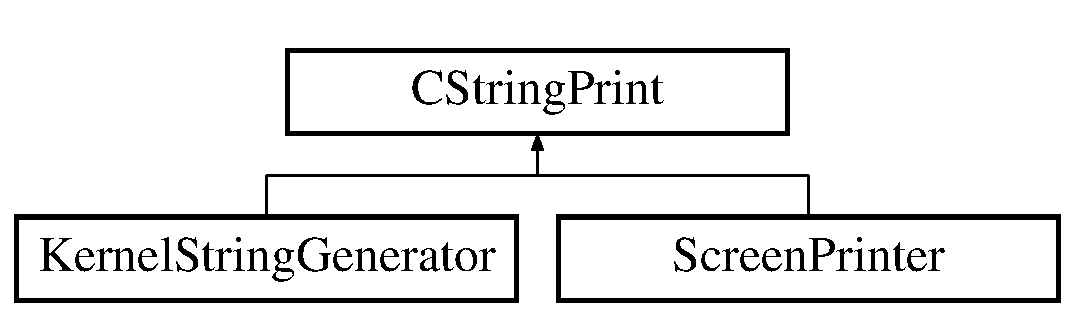
\includegraphics[height=2.000000cm]{class_c_string_print}
\end{center}
\end{figure}
\subsection*{Public Member Functions}
\begin{DoxyCompactItemize}
\item 
\mbox{\Hypertarget{class_c_string_print_a5ffc4491ea6865195c5163d1f83b309e}\label{class_c_string_print_a5ffc4491ea6865195c5163d1f83b309e}} 
void {\bfseries Print} (const char $\ast$format,...)
\item 
\mbox{\Hypertarget{class_c_string_print_aa59dd1d5fd21a71f0ccb2c9bc3adb05b}\label{class_c_string_print_aa59dd1d5fd21a71f0ccb2c9bc3adb05b}} 
void {\bfseries Print\+List} (const char $\ast$format, va\+\_\+list \&params)
\end{DoxyCompactItemize}
\subsection*{Static Public Member Functions}
\begin{DoxyCompactItemize}
\item 
\mbox{\Hypertarget{class_c_string_print_ad0fbb4a5886e3eb0f814046e76ded7d9}\label{class_c_string_print_ad0fbb4a5886e3eb0f814046e76ded7d9}} 
static bool {\bfseries Is\+Digit} (char c)
\item 
\mbox{\Hypertarget{class_c_string_print_a7fc2eff4d7f56cb742d61840c6529a1e}\label{class_c_string_print_a7fc2eff4d7f56cb742d61840c6529a1e}} 
static int {\bfseries Length\+Of} (const char $\ast$s)
\end{DoxyCompactItemize}
\subsection*{Protected Member Functions}
\begin{DoxyCompactItemize}
\item 
\mbox{\Hypertarget{class_c_string_print_a80897c8c98fcf5047730b82d5a029098}\label{class_c_string_print_a80897c8c98fcf5047730b82d5a029098}} 
virtual void {\bfseries Print\+Out} (const char $\ast$data, int length)=0
\end{DoxyCompactItemize}
\subsection*{Private Member Functions}
\begin{DoxyCompactItemize}
\item 
\mbox{\Hypertarget{class_c_string_print_a7d44210a9575d0951641e215dcf08d69}\label{class_c_string_print_a7d44210a9575d0951641e215dcf08d69}} 
int {\bfseries Parse\+Format} (va\+\_\+list \&params, const char $\ast$format)
\end{DoxyCompactItemize}


The documentation for this class was generated from the following files\+:\begin{DoxyCompactItemize}
\item 
tools.\+h\item 
tools.\+cpp\end{DoxyCompactItemize}

\hypertarget{class_i_p_c___service_1_1_userspace_provider_1_1_data}{}\section{I\+P\+C\+\_\+\+Service\+:\+:Userspace\+Provider\+:\+:Data Class Reference}
\label{class_i_p_c___service_1_1_userspace_provider_1_1_data}\index{I\+P\+C\+\_\+\+Service\+::\+Userspace\+Provider\+::\+Data@{I\+P\+C\+\_\+\+Service\+::\+Userspace\+Provider\+::\+Data}}
Inheritance diagram for I\+P\+C\+\_\+\+Service\+:\+:Userspace\+Provider\+:\+:Data\+:\begin{figure}[H]
\begin{center}
\leavevmode
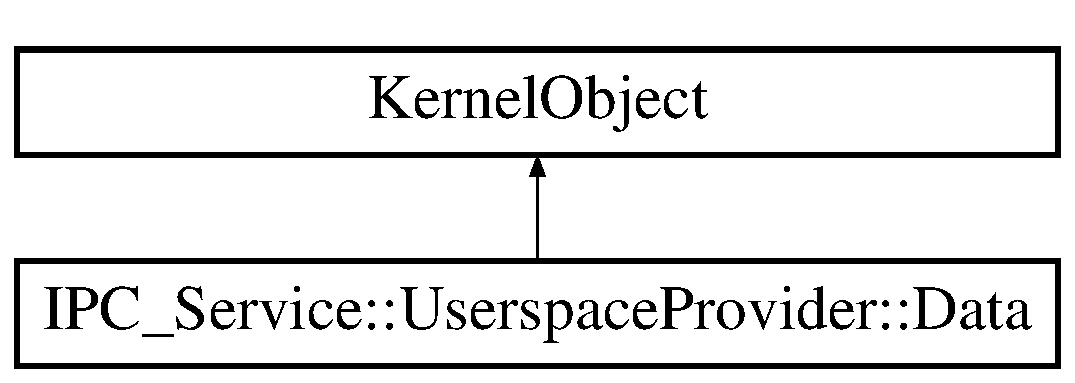
\includegraphics[height=2.000000cm]{class_i_p_c___service_1_1_userspace_provider_1_1_data}
\end{center}
\end{figure}
\subsection*{Public Member Functions}
\begin{DoxyCompactItemize}
\item 
\mbox{\Hypertarget{class_i_p_c___service_1_1_userspace_provider_1_1_data_a6fe54b26918c542ebceb4a2d32964975}\label{class_i_p_c___service_1_1_userspace_provider_1_1_data_a6fe54b26918c542ebceb4a2d32964975}} 
const char $\ast$ {\bfseries Get\+Class\+Name} (U\+Int32 level)
\item 
\mbox{\Hypertarget{class_i_p_c___service_1_1_userspace_provider_1_1_data_ae630842724e94b4fd389d2d60c00a4bf}\label{class_i_p_c___service_1_1_userspace_provider_1_1_data_ae630842724e94b4fd389d2d60c00a4bf}} 
{\bfseries Data} (int type, \hyperlink{class_ipc_endpoint}{Ipc\+Endpoint} $\ast$connection, \hyperlink{class_kernel_buffer_memory}{Kernel\+Buffer\+Memory} $\ast$message, \hyperlink{class_kernel_object}{Kernel\+Object} $\ast$owner)
\item 
\mbox{\Hypertarget{class_i_p_c___service_1_1_userspace_provider_1_1_data_ad2ea3d7a2e440cc2592a51b287646fc2}\label{class_i_p_c___service_1_1_userspace_provider_1_1_data_ad2ea3d7a2e440cc2592a51b287646fc2}} 
void {\bfseries Save} (U\+Int64 $\ast$output)
\end{DoxyCompactItemize}
\subsection*{Private Attributes}
\begin{DoxyCompactItemize}
\item 
\mbox{\Hypertarget{class_i_p_c___service_1_1_userspace_provider_1_1_data_aa3501006f181884717697d1658ec89b3}\label{class_i_p_c___service_1_1_userspace_provider_1_1_data_aa3501006f181884717697d1658ec89b3}} 
int {\bfseries \+\_\+type}
\item 
\mbox{\Hypertarget{class_i_p_c___service_1_1_userspace_provider_1_1_data_a8972258a8d6d54fcd55cb3544496eaf8}\label{class_i_p_c___service_1_1_userspace_provider_1_1_data_a8972258a8d6d54fcd55cb3544496eaf8}} 
\hyperlink{class_ipc_endpoint}{Ipc\+Endpoint} $\ast$ {\bfseries \+\_\+endpoint}
\item 
\mbox{\Hypertarget{class_i_p_c___service_1_1_userspace_provider_1_1_data_a8ba7300c495011bfc0930c2a58168d76}\label{class_i_p_c___service_1_1_userspace_provider_1_1_data_a8ba7300c495011bfc0930c2a58168d76}} 
\hyperlink{class_kernel_buffer_memory}{Kernel\+Buffer\+Memory} $\ast$ {\bfseries \+\_\+memory}
\item 
\mbox{\Hypertarget{class_i_p_c___service_1_1_userspace_provider_1_1_data_af56838f51c3f581ebd3175ce919dde28}\label{class_i_p_c___service_1_1_userspace_provider_1_1_data_af56838f51c3f581ebd3175ce919dde28}} 
\hyperlink{class_kernel_object}{Kernel\+Object} $\ast$ {\bfseries \+\_\+source}
\end{DoxyCompactItemize}
\subsection*{Additional Inherited Members}


The documentation for this class was generated from the following file\+:\begin{DoxyCompactItemize}
\item 
I\+P\+C\+\_\+\+Service.\+cpp\end{DoxyCompactItemize}

\hypertarget{class_default_v_g_a_console_driver}{}\section{Default\+V\+G\+A\+Console\+Driver Class Reference}
\label{class_default_v_g_a_console_driver}\index{Default\+V\+G\+A\+Console\+Driver@{Default\+V\+G\+A\+Console\+Driver}}
Inheritance diagram for Default\+V\+G\+A\+Console\+Driver\+:\begin{figure}[H]
\begin{center}
\leavevmode
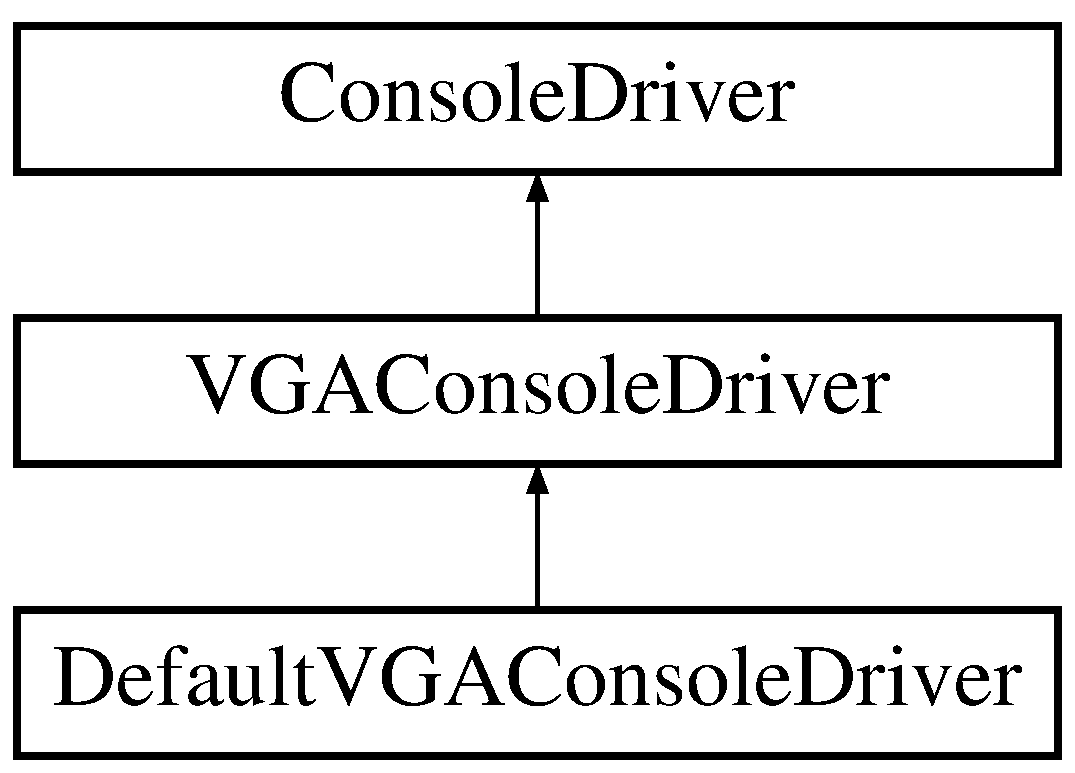
\includegraphics[height=3.000000cm]{class_default_v_g_a_console_driver}
\end{center}
\end{figure}
\subsection*{Public Member Functions}
\begin{DoxyCompactItemize}
\item 
\mbox{\Hypertarget{class_default_v_g_a_console_driver_a3d64c219ba74aaf8c488d4c2c5fef810}\label{class_default_v_g_a_console_driver_a3d64c219ba74aaf8c488d4c2c5fef810}} 
void {\bfseries Set\+Cursor} (int x, int y)
\item 
\mbox{\Hypertarget{class_default_v_g_a_console_driver_a3aef71265888b16365571d7ab741721a}\label{class_default_v_g_a_console_driver_a3aef71265888b16365571d7ab741721a}} 
void {\bfseries Get\+Cursor} (int $\ast$x, int $\ast$y)
\item 
\mbox{\Hypertarget{class_default_v_g_a_console_driver_a8e51ae9b29d13477075669d4f90cd053}\label{class_default_v_g_a_console_driver_a8e51ae9b29d13477075669d4f90cd053}} 
void {\bfseries Set\+Cursor\+Enabled} (bool enabled)
\end{DoxyCompactItemize}
\subsection*{Private Attributes}
\begin{DoxyCompactItemize}
\item 
\mbox{\Hypertarget{class_default_v_g_a_console_driver_a3005e5cf0d599a5ff0eec440c60d81e0}\label{class_default_v_g_a_console_driver_a3005e5cf0d599a5ff0eec440c60d81e0}} 
bool {\bfseries set}
\item 
\mbox{\Hypertarget{class_default_v_g_a_console_driver_ab7cdc0053a6a7be8618622b9a871e496}\label{class_default_v_g_a_console_driver_ab7cdc0053a6a7be8618622b9a871e496}} 
int {\bfseries got}
\end{DoxyCompactItemize}


The documentation for this class was generated from the following file\+:\begin{DoxyCompactItemize}
\item 
Video\+\_\+\+Multiboot.\+cpp\end{DoxyCompactItemize}

\hypertarget{class_kernel_object___internal_1_1_destruction_watcher_handle}{}\section{Kernel\+Object\+\_\+\+Internal\+:\+:Destruction\+Watcher\+Handle Class Reference}
\label{class_kernel_object___internal_1_1_destruction_watcher_handle}\index{Kernel\+Object\+\_\+\+Internal\+::\+Destruction\+Watcher\+Handle@{Kernel\+Object\+\_\+\+Internal\+::\+Destruction\+Watcher\+Handle}}
Inheritance diagram for Kernel\+Object\+\_\+\+Internal\+:\+:Destruction\+Watcher\+Handle\+:\begin{figure}[H]
\begin{center}
\leavevmode
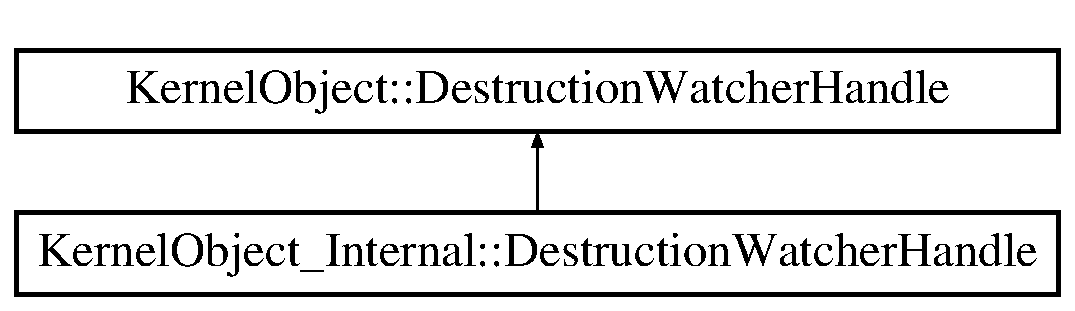
\includegraphics[height=2.000000cm]{class_kernel_object___internal_1_1_destruction_watcher_handle}
\end{center}
\end{figure}
\subsection*{Public Member Functions}
\begin{DoxyCompactItemize}
\item 
\mbox{\Hypertarget{class_kernel_object___internal_1_1_destruction_watcher_handle_a22c59517d57b899e9c8b8e03ab1323a6}\label{class_kernel_object___internal_1_1_destruction_watcher_handle_a22c59517d57b899e9c8b8e03ab1323a6}} 
{\bfseries Destruction\+Watcher\+Handle} (\hyperlink{class_kernel_object_1_1_destruction_watcher_handle}{Kernel\+Object\+::\+Destruction\+Watcher\+Handle} $\ast$$\ast$start, \hyperlink{class_kernel_object_1_1_destruction_watcher_handle}{Kernel\+Object\+::\+Destruction\+Watcher\+Handle} $\ast$$\ast$end, \hyperlink{classbicycle_1_1function}{bicycle\+::function}$<$ void(void)$>$ on\+Destroy)
\item 
\mbox{\Hypertarget{class_kernel_object___internal_1_1_destruction_watcher_handle_ac4a99a8fcb2e0e36a9ed424f1dacf18b}\label{class_kernel_object___internal_1_1_destruction_watcher_handle_ac4a99a8fcb2e0e36a9ed424f1dacf18b}} 
void {\bfseries Run} (void)
\end{DoxyCompactItemize}
\subsection*{Private Attributes}
\begin{DoxyCompactItemize}
\item 
\mbox{\Hypertarget{class_kernel_object___internal_1_1_destruction_watcher_handle_ac7ea6e6fbd9c94f2ac9f00553caaa455}\label{class_kernel_object___internal_1_1_destruction_watcher_handle_ac7ea6e6fbd9c94f2ac9f00553caaa455}} 
\hyperlink{class_kernel_object_1_1_destruction_watcher_handle}{Kernel\+Object\+::\+Destruction\+Watcher\+Handle} $\ast$$\ast$ {\bfseries \+\_\+start}
\item 
\mbox{\Hypertarget{class_kernel_object___internal_1_1_destruction_watcher_handle_ac2dc223fe682c6bfaa04207ee918e1c9}\label{class_kernel_object___internal_1_1_destruction_watcher_handle_ac2dc223fe682c6bfaa04207ee918e1c9}} 
\hyperlink{class_kernel_object_1_1_destruction_watcher_handle}{Kernel\+Object\+::\+Destruction\+Watcher\+Handle} $\ast$$\ast$ {\bfseries \+\_\+end}
\item 
\mbox{\Hypertarget{class_kernel_object___internal_1_1_destruction_watcher_handle_a30d3f4a11a58e083c1e6511134847201}\label{class_kernel_object___internal_1_1_destruction_watcher_handle_a30d3f4a11a58e083c1e6511134847201}} 
\hyperlink{class_kernel_object_1_1_destruction_watcher_handle}{Kernel\+Object\+::\+Destruction\+Watcher\+Handle} $\ast$ {\bfseries \+\_\+last}
\item 
\mbox{\Hypertarget{class_kernel_object___internal_1_1_destruction_watcher_handle_a592ff0484d078e959d8666c8814060b5}\label{class_kernel_object___internal_1_1_destruction_watcher_handle_a592ff0484d078e959d8666c8814060b5}} 
\hyperlink{class_kernel_object_1_1_destruction_watcher_handle}{Kernel\+Object\+::\+Destruction\+Watcher\+Handle} $\ast$ {\bfseries \+\_\+next}
\item 
\mbox{\Hypertarget{class_kernel_object___internal_1_1_destruction_watcher_handle_a16a94d405963ef9aa0ba855a2cc939c1}\label{class_kernel_object___internal_1_1_destruction_watcher_handle_a16a94d405963ef9aa0ba855a2cc939c1}} 
\hyperlink{classbicycle_1_1function}{bicycle\+::function}$<$ void(void)$>$ {\bfseries \+\_\+destroy}
\end{DoxyCompactItemize}


The documentation for this class was generated from the following file\+:\begin{DoxyCompactItemize}
\item 
Kernel\+Object.\+cpp\end{DoxyCompactItemize}

\hypertarget{class_kernel_object_1_1_destruction_watcher_handle}{}\section{Kernel\+Object\+:\+:Destruction\+Watcher\+Handle Class Reference}
\label{class_kernel_object_1_1_destruction_watcher_handle}\index{Kernel\+Object\+::\+Destruction\+Watcher\+Handle@{Kernel\+Object\+::\+Destruction\+Watcher\+Handle}}
Inheritance diagram for Kernel\+Object\+:\+:Destruction\+Watcher\+Handle\+:\begin{figure}[H]
\begin{center}
\leavevmode
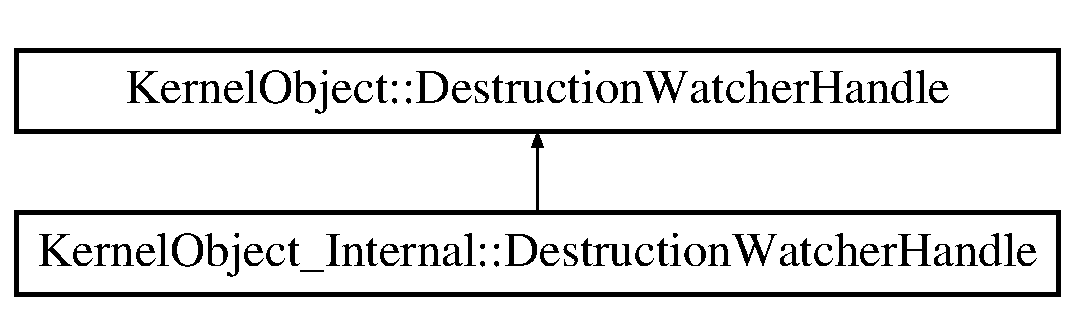
\includegraphics[height=2.000000cm]{class_kernel_object_1_1_destruction_watcher_handle}
\end{center}
\end{figure}


The documentation for this class was generated from the following file\+:\begin{DoxyCompactItemize}
\item 
Kernel\+Object.\+h\end{DoxyCompactItemize}

\hypertarget{class_p_c_i_1_1_device}{}\section{P\+CI\+:\+:Device Class Reference}
\label{class_p_c_i_1_1_device}\index{P\+C\+I\+::\+Device@{P\+C\+I\+::\+Device}}
Inheritance diagram for P\+CI\+:\+:Device\+:\begin{figure}[H]
\begin{center}
\leavevmode
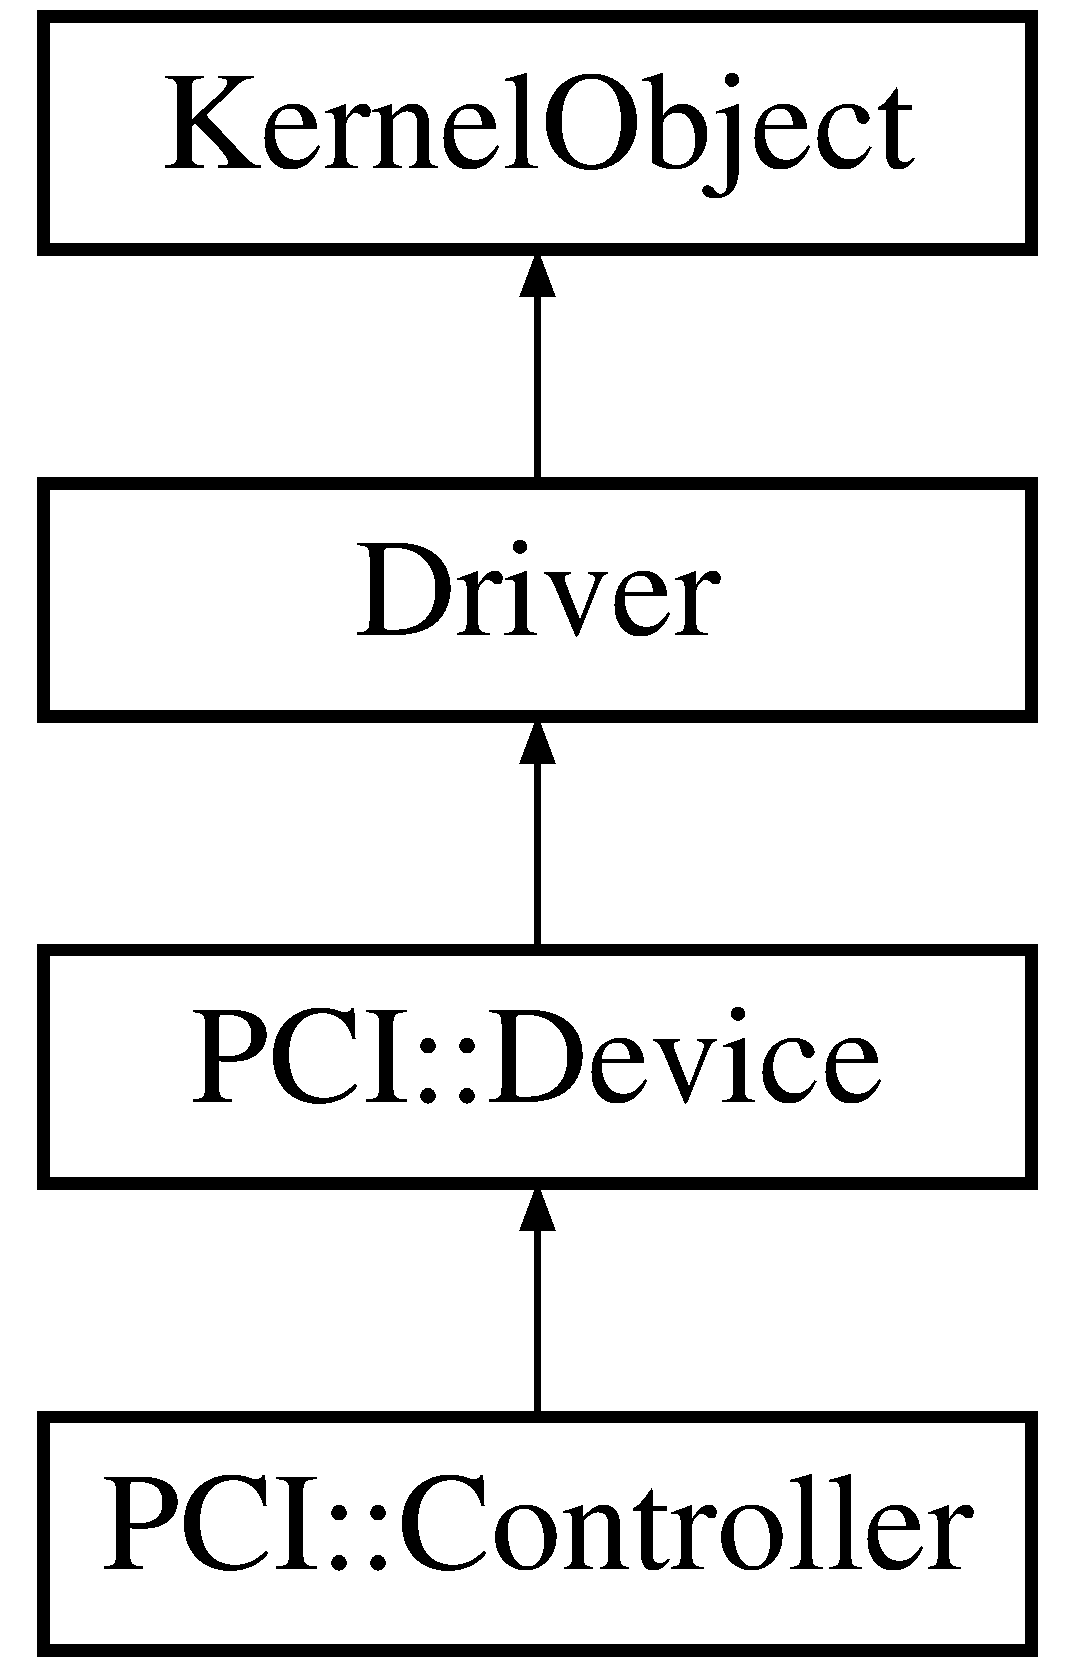
\includegraphics[height=4.000000cm]{class_p_c_i_1_1_device}
\end{center}
\end{figure}
\subsection*{Public Member Functions}
\begin{DoxyCompactItemize}
\item 
\mbox{\Hypertarget{class_p_c_i_1_1_device_a4cd01dd207da8bec0782cea685ee3921}\label{class_p_c_i_1_1_device_a4cd01dd207da8bec0782cea685ee3921}} 
const char $\ast$ {\bfseries Get\+Class\+Name} (U\+Int32 level)
\item 
\mbox{\Hypertarget{class_p_c_i_1_1_device_a8c802a13f70f87f54515e18582697a7a}\label{class_p_c_i_1_1_device_a8c802a13f70f87f54515e18582697a7a}} 
{\bfseries Device} (const char $\ast$name, U\+Int8 bus, U\+Int8 device, U\+Int8 function)
\item 
\mbox{\Hypertarget{class_p_c_i_1_1_device_ac156bded5416c390d6473b7ff10930f7}\label{class_p_c_i_1_1_device_ac156bded5416c390d6473b7ff10930f7}} 
U\+Int8 {\bfseries Bus} (void)
\item 
\mbox{\Hypertarget{class_p_c_i_1_1_device_a4ca1d7ad6b1bbcdb26ce9c503be49988}\label{class_p_c_i_1_1_device_a4ca1d7ad6b1bbcdb26ce9c503be49988}} 
U\+Int8 {\bfseries P\+C\+I\+Device} (void)
\item 
\mbox{\Hypertarget{class_p_c_i_1_1_device_a2693e3d5351ed5e885130ec69009c2e6}\label{class_p_c_i_1_1_device_a2693e3d5351ed5e885130ec69009c2e6}} 
U\+Int8 {\bfseries Function} (void)
\item 
\mbox{\Hypertarget{class_p_c_i_1_1_device_af7ad0b76bfffb0530005d5bcfe45133b}\label{class_p_c_i_1_1_device_af7ad0b76bfffb0530005d5bcfe45133b}} 
U\+Int16 {\bfseries Vendor\+ID} (void)
\item 
\mbox{\Hypertarget{class_p_c_i_1_1_device_aa87d2a176e119d83dd028ca23e0eca97}\label{class_p_c_i_1_1_device_aa87d2a176e119d83dd028ca23e0eca97}} 
U\+Int16 {\bfseries Device\+ID} (void)
\item 
\mbox{\Hypertarget{class_p_c_i_1_1_device_a05ea166817d3dbd1cb1156cf9af1310c}\label{class_p_c_i_1_1_device_a05ea166817d3dbd1cb1156cf9af1310c}} 
U\+Int8 {\bfseries Header\+Type} (void)
\item 
\mbox{\Hypertarget{class_p_c_i_1_1_device_a2b684ca6a69959339e2b7b48efc0bba5}\label{class_p_c_i_1_1_device_a2b684ca6a69959339e2b7b48efc0bba5}} 
U\+Int8 {\bfseries Base\+Class} (void)
\item 
\mbox{\Hypertarget{class_p_c_i_1_1_device_ab2f26fd2c025a104052c32ef40d1ca47}\label{class_p_c_i_1_1_device_ab2f26fd2c025a104052c32ef40d1ca47}} 
U\+Int8 {\bfseries Sub\+Class} (void)
\item 
\mbox{\Hypertarget{class_p_c_i_1_1_device_a4b8d0c211e4b8722397574408ad93bc6}\label{class_p_c_i_1_1_device_a4b8d0c211e4b8722397574408ad93bc6}} 
U\+Int32 {\bfseries Read\+B\+AR} (U\+Int8 bar)
\item 
\mbox{\Hypertarget{class_p_c_i_1_1_device_acb6992e4a37c36efdda5d7f2de916166}\label{class_p_c_i_1_1_device_acb6992e4a37c36efdda5d7f2de916166}} 
U\+Int16 {\bfseries Status} (void)
\item 
\mbox{\Hypertarget{class_p_c_i_1_1_device_abac79f8a35c4cec8aae8fa0ab060baf9}\label{class_p_c_i_1_1_device_abac79f8a35c4cec8aae8fa0ab060baf9}} 
U\+Int32 {\bfseries Read\+P\+C\+I\+Register} (U\+Int8 reg)
\item 
\mbox{\Hypertarget{class_p_c_i_1_1_device_a106d53580b7102da5e38e578ae7af00c}\label{class_p_c_i_1_1_device_a106d53580b7102da5e38e578ae7af00c}} 
void {\bfseries Write\+P\+C\+I\+Register} (U\+Int8 reg, U\+Int32 value)
\item 
\mbox{\Hypertarget{class_p_c_i_1_1_device_a323b4199e204596a1b35e83e6aa539b4}\label{class_p_c_i_1_1_device_a323b4199e204596a1b35e83e6aa539b4}} 
\hyperlink{class_interrupts}{Interrupts} $\ast$ {\bfseries Interrupt\+Source} (void)
\end{DoxyCompactItemize}
\subsection*{Private Attributes}
\begin{DoxyCompactItemize}
\item 
\mbox{\Hypertarget{class_p_c_i_1_1_device_a9b6471f14a9232bf92dba05df8cc4b2e}\label{class_p_c_i_1_1_device_a9b6471f14a9232bf92dba05df8cc4b2e}} 
U\+Int8 {\bfseries \+\_\+bus}
\item 
\mbox{\Hypertarget{class_p_c_i_1_1_device_a6ed31c0a3f573f63db71619c804212d5}\label{class_p_c_i_1_1_device_a6ed31c0a3f573f63db71619c804212d5}} 
U\+Int8 {\bfseries \+\_\+device}
\item 
\mbox{\Hypertarget{class_p_c_i_1_1_device_a4f27b1199ccddbe3bb3cb08df70c7267}\label{class_p_c_i_1_1_device_a4f27b1199ccddbe3bb3cb08df70c7267}} 
U\+Int8 {\bfseries \+\_\+function}
\end{DoxyCompactItemize}
\subsection*{Additional Inherited Members}


The documentation for this class was generated from the following files\+:\begin{DoxyCompactItemize}
\item 
pci.\+h\item 
pci.\+cpp\end{DoxyCompactItemize}

\hypertarget{class_i_s_o9660_driver_1_1_directory_entry}{}\section{I\+S\+O9660\+Driver\+:\+:Directory\+Entry Class Reference}
\label{class_i_s_o9660_driver_1_1_directory_entry}\index{I\+S\+O9660\+Driver\+::\+Directory\+Entry@{I\+S\+O9660\+Driver\+::\+Directory\+Entry}}
Inheritance diagram for I\+S\+O9660\+Driver\+:\+:Directory\+Entry\+:\begin{figure}[H]
\begin{center}
\leavevmode
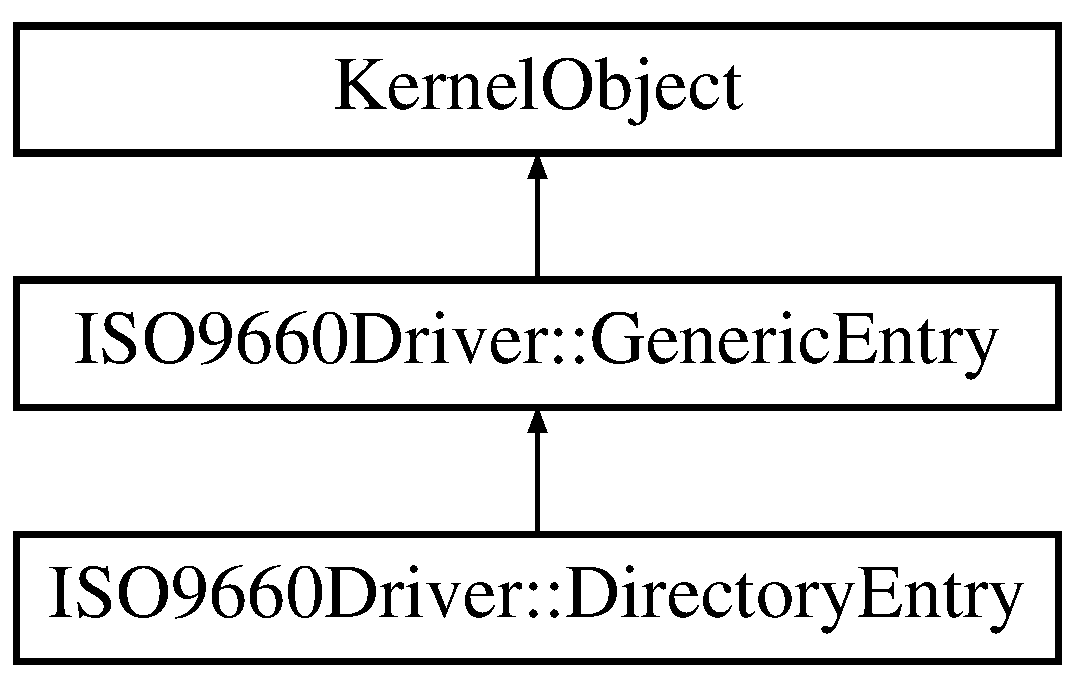
\includegraphics[height=3.000000cm]{class_i_s_o9660_driver_1_1_directory_entry}
\end{center}
\end{figure}
\subsection*{Public Member Functions}
\begin{DoxyCompactItemize}
\item 
\mbox{\Hypertarget{class_i_s_o9660_driver_1_1_directory_entry_a3b7991145db6160135509659a40bec42}\label{class_i_s_o9660_driver_1_1_directory_entry_a3b7991145db6160135509659a40bec42}} 
const char $\ast$ {\bfseries Get\+Class\+Name} (U\+Int32 level)
\item 
\mbox{\Hypertarget{class_i_s_o9660_driver_1_1_directory_entry_a0ffa97f591a6f9b68a9167d56a49dc8b}\label{class_i_s_o9660_driver_1_1_directory_entry_a0ffa97f591a6f9b68a9167d56a49dc8b}} 
{\bfseries Directory\+Entry} (Directory\+Record $\ast$record)
\item 
\mbox{\Hypertarget{class_i_s_o9660_driver_1_1_directory_entry_ad70d802668b01cc163a4a79a7f1d3228}\label{class_i_s_o9660_driver_1_1_directory_entry_ad70d802668b01cc163a4a79a7f1d3228}} 
bool {\bfseries Loaded} (void)
\item 
\mbox{\Hypertarget{class_i_s_o9660_driver_1_1_directory_entry_a2f0a3cc8a0bf887e2d2aa5c525ee7959}\label{class_i_s_o9660_driver_1_1_directory_entry_a2f0a3cc8a0bf887e2d2aa5c525ee7959}} 
void {\bfseries Parse} (U\+Int64 \&node\+Counter, void $\ast$data)
\item 
\mbox{\Hypertarget{class_i_s_o9660_driver_1_1_directory_entry_ac06665e7497151be5c73f391abc43a06}\label{class_i_s_o9660_driver_1_1_directory_entry_ac06665e7497151be5c73f391abc43a06}} 
\hyperlink{class_kernel_array}{Kernel\+Array} $\ast$ {\bfseries Entries} (void)
\item 
\mbox{\Hypertarget{class_i_s_o9660_driver_1_1_directory_entry_afe44ce377d28399d630aae0366fd4a93}\label{class_i_s_o9660_driver_1_1_directory_entry_afe44ce377d28399d630aae0366fd4a93}} 
\hyperlink{class_i_s_o9660_driver_1_1_generic_entry}{Generic\+Entry} $\ast$ {\bfseries Search\+Entry} (U\+Int32 node)
\item 
\mbox{\Hypertarget{class_i_s_o9660_driver_1_1_directory_entry_a00ddae7aa76e86c00ddcc7d363e09679}\label{class_i_s_o9660_driver_1_1_directory_entry_a00ddae7aa76e86c00ddcc7d363e09679}} 
\hyperlink{class_i_s_o9660_driver_1_1_generic_entry}{Generic\+Entry} $\ast$ {\bfseries Search\+Entry} (\hyperlink{class_kernel_string}{Kernel\+String} $\ast$name)
\item 
\mbox{\Hypertarget{class_i_s_o9660_driver_1_1_directory_entry_ac1c570c8d5d9132d77da154a22f1c5af}\label{class_i_s_o9660_driver_1_1_directory_entry_ac1c570c8d5d9132d77da154a22f1c5af}} 
\hyperlink{class_i_s_o9660_driver_1_1_generic_entry}{Generic\+Entry} $\ast$ {\bfseries Find\+Node} (U\+Int32 node)
\end{DoxyCompactItemize}
\subsection*{Static Private Member Functions}
\begin{DoxyCompactItemize}
\item 
\mbox{\Hypertarget{class_i_s_o9660_driver_1_1_directory_entry_a72fb6153bc7150d744e16447521996ad}\label{class_i_s_o9660_driver_1_1_directory_entry_a72fb6153bc7150d744e16447521996ad}} 
static \hyperlink{class_i_s_o9660_driver_1_1_generic_entry}{Generic\+Entry} $\ast$ {\bfseries Create} (U\+Int64 \&node\+Counter, Directory\+Record $\ast$record)
\end{DoxyCompactItemize}
\subsection*{Private Attributes}
\begin{DoxyCompactItemize}
\item 
\mbox{\Hypertarget{class_i_s_o9660_driver_1_1_directory_entry_af72d3107d8492883fe27ae043fda5c2b}\label{class_i_s_o9660_driver_1_1_directory_entry_af72d3107d8492883fe27ae043fda5c2b}} 
\hyperlink{class_kernel_array}{Kernel\+Array} $\ast$ {\bfseries \+\_\+entries}
\end{DoxyCompactItemize}
\subsection*{Additional Inherited Members}


The documentation for this class was generated from the following file\+:\begin{DoxyCompactItemize}
\item 
fs\+\_\+iso9660.\+cpp\end{DoxyCompactItemize}

\hypertarget{class_dispatch_group}{}\section{Dispatch\+Group Class Reference}
\label{class_dispatch_group}\index{Dispatch\+Group@{Dispatch\+Group}}
Inheritance diagram for Dispatch\+Group\+:\begin{figure}[H]
\begin{center}
\leavevmode
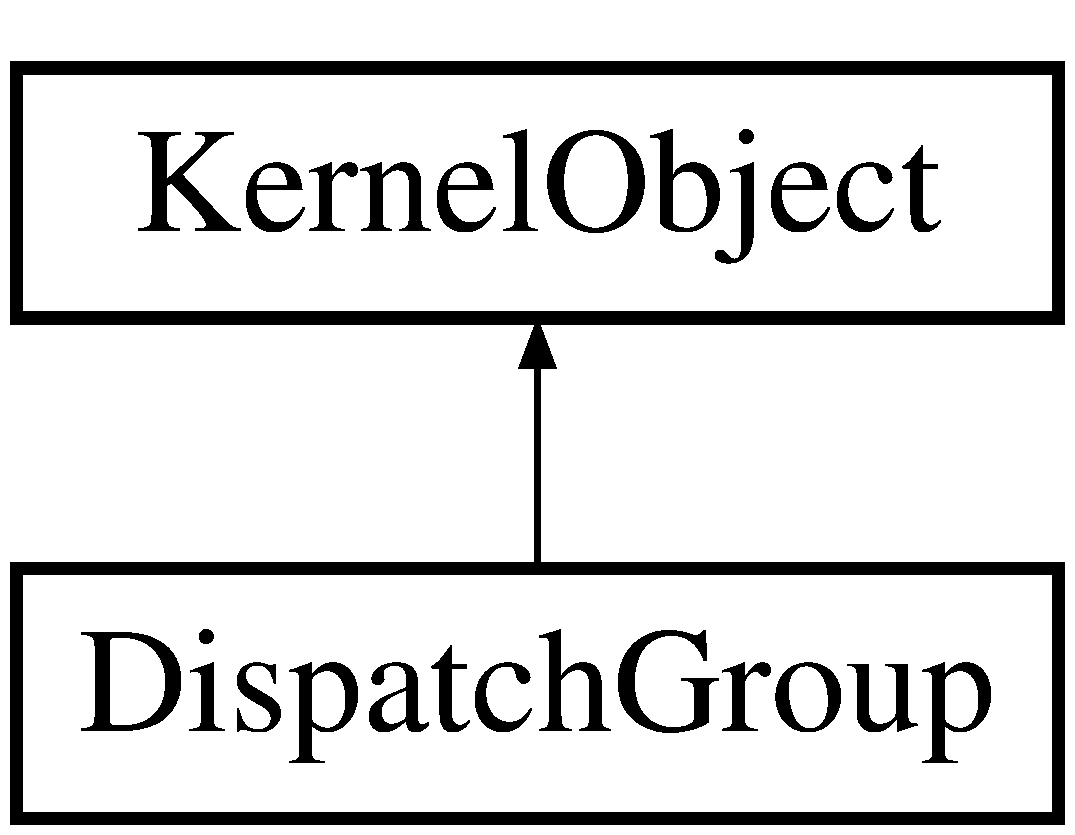
\includegraphics[height=2.000000cm]{class_dispatch_group}
\end{center}
\end{figure}
\subsection*{Classes}
\begin{DoxyCompactItemize}
\item 
class \hyperlink{class_dispatch_group_1_1_block}{Block}
\end{DoxyCompactItemize}
\subsection*{Public Member Functions}
\begin{DoxyCompactItemize}
\item 
\mbox{\Hypertarget{class_dispatch_group_afc5d3ca0a4653b8086ed75d2c9e4d189}\label{class_dispatch_group_afc5d3ca0a4653b8086ed75d2c9e4d189}} 
const char $\ast$ {\bfseries Get\+Class\+Name} (U\+Int32 level)
\item 
\mbox{\Hypertarget{class_dispatch_group_a7b46159a6164d8766a7a1e76ef6afb5e}\label{class_dispatch_group_a7b46159a6164d8766a7a1e76ef6afb5e}} 
void $\ast$ {\bfseries Enter\+Or\+Timeout} (U\+Int32 microseconds\+Passed=0)
\item 
\mbox{\Hypertarget{class_dispatch_group_a91a5a5ff7c16c99dc095a3a71a6d67c1}\label{class_dispatch_group_a91a5a5ff7c16c99dc095a3a71a6d67c1}} 
void {\bfseries Exit} (void $\ast$token)
\end{DoxyCompactItemize}
\subsection*{Private Attributes}
\begin{DoxyCompactItemize}
\item 
\mbox{\Hypertarget{class_dispatch_group_addee2d352ae490c730edd60a1b9a1f44}\label{class_dispatch_group_addee2d352ae490c730edd60a1b9a1f44}} 
\hyperlink{class_hardcore_spin_lock}{Hardcore\+Spin\+Lock} {\bfseries \+\_\+lock}
\item 
\mbox{\Hypertarget{class_dispatch_group_aad762a4511216a55c195c9df783fce67}\label{class_dispatch_group_aad762a4511216a55c195c9df783fce67}} 
\hyperlink{class_dispatch_group_holder}{Dispatch\+Group\+Holder} $\ast$ {\bfseries \+\_\+start}
\item 
\mbox{\Hypertarget{class_dispatch_group_a6d71594707c8ea942534e1a985914b21}\label{class_dispatch_group_a6d71594707c8ea942534e1a985914b21}} 
\hyperlink{class_dispatch_group_holder}{Dispatch\+Group\+Holder} $\ast$ {\bfseries \+\_\+end}
\item 
\mbox{\Hypertarget{class_dispatch_group_a10f894ac59e3e32aa51ad8548b1f1e0f}\label{class_dispatch_group_a10f894ac59e3e32aa51ad8548b1f1e0f}} 
\hyperlink{class_dispatch_group_holder}{Dispatch\+Group\+Holder} $\ast$ {\bfseries \+\_\+current}
\end{DoxyCompactItemize}
\subsection*{Additional Inherited Members}


The documentation for this class was generated from the following files\+:\begin{DoxyCompactItemize}
\item 
Queue.\+h\item 
Queue.\+cpp\end{DoxyCompactItemize}

\hypertarget{class_dispatch_group_holder}{}\section{Dispatch\+Group\+Holder Class Reference}
\label{class_dispatch_group_holder}\index{Dispatch\+Group\+Holder@{Dispatch\+Group\+Holder}}
Inheritance diagram for Dispatch\+Group\+Holder\+:\begin{figure}[H]
\begin{center}
\leavevmode
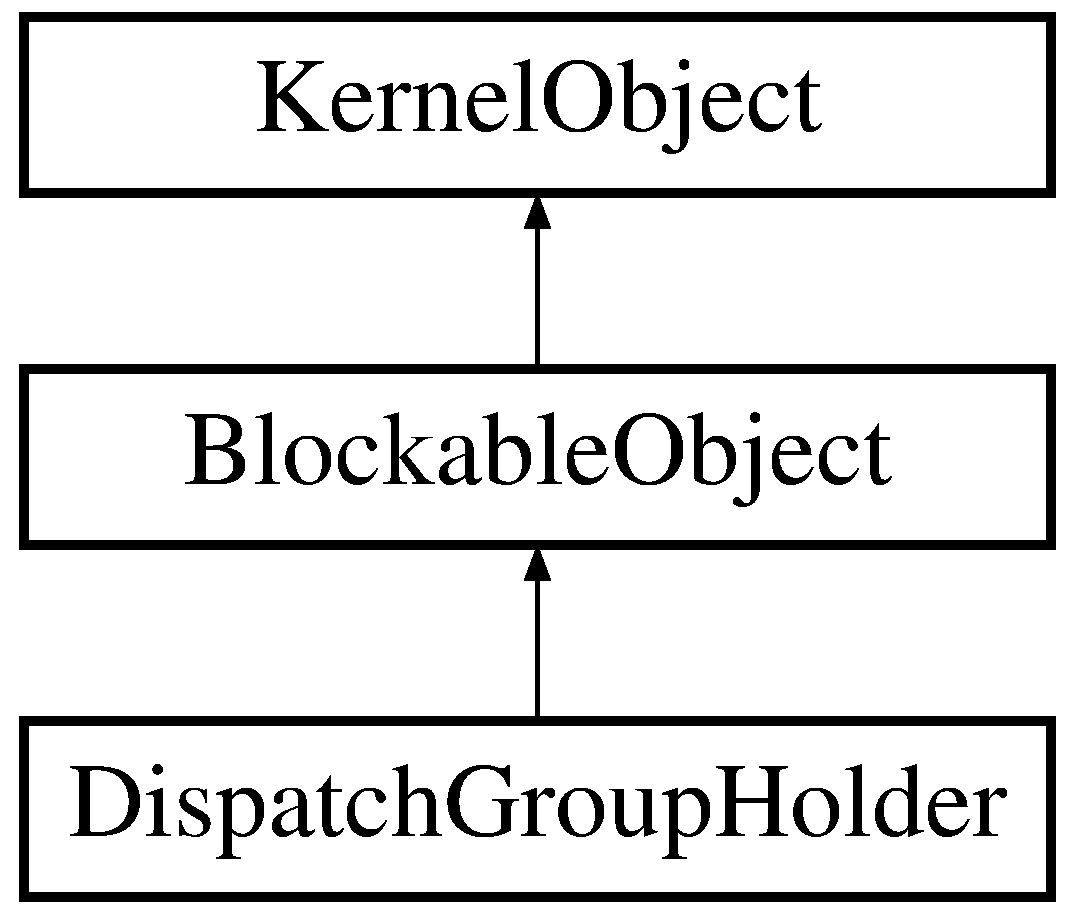
\includegraphics[height=3.000000cm]{class_dispatch_group_holder}
\end{center}
\end{figure}
\subsection*{Public Member Functions}
\begin{DoxyCompactItemize}
\item 
\mbox{\Hypertarget{class_dispatch_group_holder_aae21b4b1b4450fbe91c72f23c3c05740}\label{class_dispatch_group_holder_aae21b4b1b4450fbe91c72f23c3c05740}} 
const char $\ast$ {\bfseries Get\+Class\+Name} (U\+Int32 level)
\item 
\mbox{\Hypertarget{class_dispatch_group_holder_ab8fbf08463a7fbc1cc5e45907f8c050c}\label{class_dispatch_group_holder_ab8fbf08463a7fbc1cc5e45907f8c050c}} 
{\bfseries Dispatch\+Group\+Holder} (\hyperlink{class_dispatch_group_holder}{Dispatch\+Group\+Holder} $\ast$$\ast$start, \hyperlink{class_dispatch_group_holder}{Dispatch\+Group\+Holder} $\ast$$\ast$end)
\item 
\mbox{\Hypertarget{class_dispatch_group_holder_a2c804da5523078a19dd0df85314805ea}\label{class_dispatch_group_holder_a2c804da5523078a19dd0df85314805ea}} 
\hyperlink{class_blockable_object}{Blockable\+Object} $\ast$ {\bfseries After\+These} (void)
\item 
\mbox{\Hypertarget{class_dispatch_group_holder_aa8d9db75b9364a749adff5aaf5f2641d}\label{class_dispatch_group_holder_aa8d9db75b9364a749adff5aaf5f2641d}} 
void {\bfseries Completed} (void)
\end{DoxyCompactItemize}
\subsection*{Private Attributes}
\begin{DoxyCompactItemize}
\item 
\mbox{\Hypertarget{class_dispatch_group_holder_a4a9eae28e44db90d2a42378d6b9fc0e1}\label{class_dispatch_group_holder_a4a9eae28e44db90d2a42378d6b9fc0e1}} 
\hyperlink{class_dispatch_group_holder}{Dispatch\+Group\+Holder} $\ast$$\ast$ {\bfseries \+\_\+start}
\item 
\mbox{\Hypertarget{class_dispatch_group_holder_a263959802537c48cb097bf85d327421c}\label{class_dispatch_group_holder_a263959802537c48cb097bf85d327421c}} 
\hyperlink{class_dispatch_group_holder}{Dispatch\+Group\+Holder} $\ast$$\ast$ {\bfseries \+\_\+end}
\item 
\mbox{\Hypertarget{class_dispatch_group_holder_afb5567f718605a7aa5034f95797ce844}\label{class_dispatch_group_holder_afb5567f718605a7aa5034f95797ce844}} 
\hyperlink{class_dispatch_group_holder}{Dispatch\+Group\+Holder} $\ast$ {\bfseries \+\_\+last}
\item 
\mbox{\Hypertarget{class_dispatch_group_holder_a3176a6a7ccbf8ce86bb6a166e5c786aa}\label{class_dispatch_group_holder_a3176a6a7ccbf8ce86bb6a166e5c786aa}} 
\hyperlink{class_dispatch_group_holder}{Dispatch\+Group\+Holder} $\ast$ {\bfseries \+\_\+next}
\end{DoxyCompactItemize}
\subsection*{Additional Inherited Members}


The documentation for this class was generated from the following file\+:\begin{DoxyCompactItemize}
\item 
Queue.\+cpp\end{DoxyCompactItemize}

\hypertarget{class_dispatch_queue}{}\section{Dispatch\+Queue Class Reference}
\label{class_dispatch_queue}\index{Dispatch\+Queue@{Dispatch\+Queue}}
Inheritance diagram for Dispatch\+Queue\+:\begin{figure}[H]
\begin{center}
\leavevmode
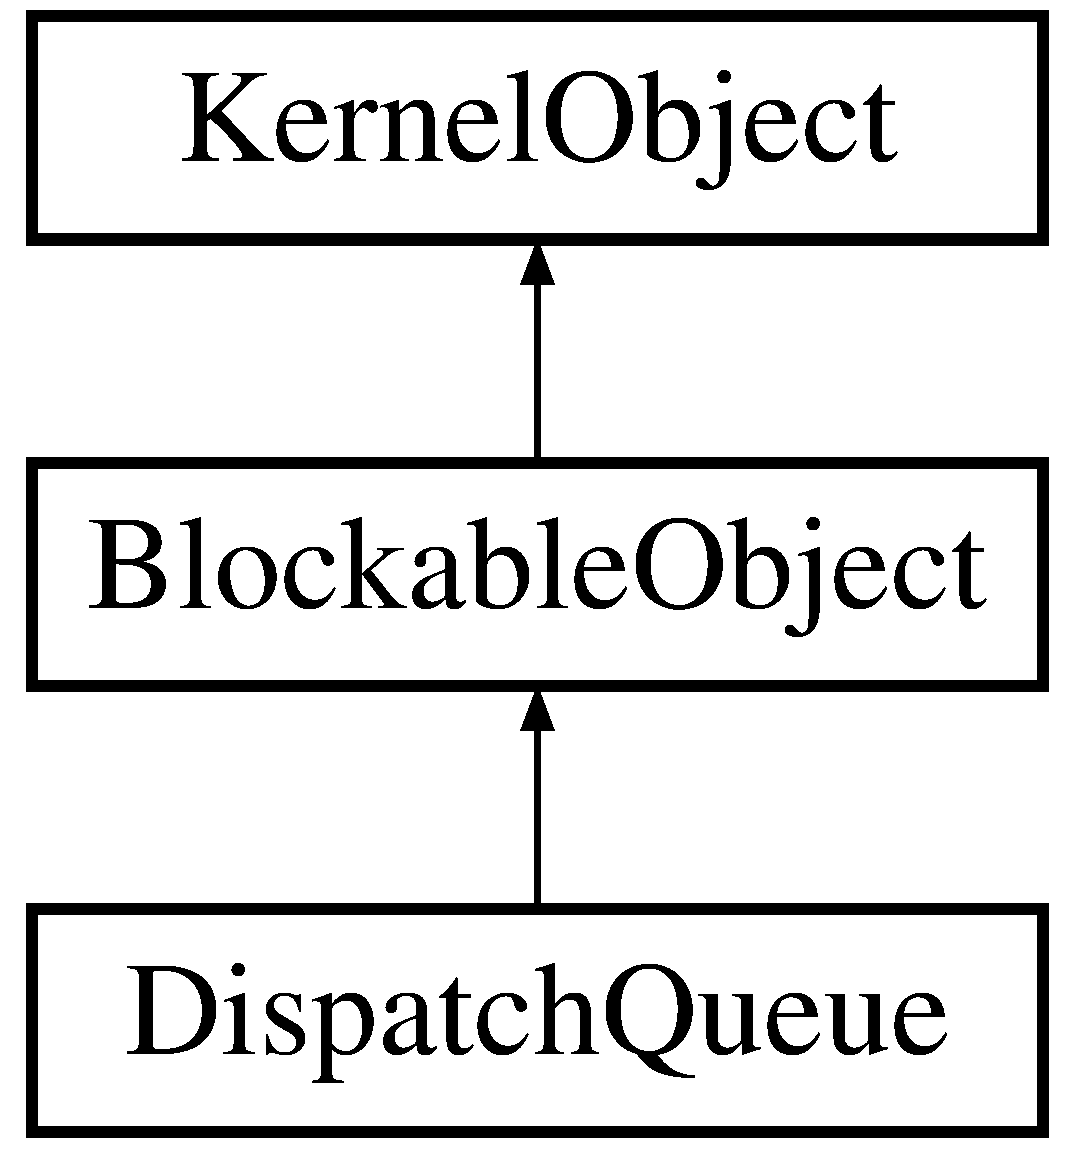
\includegraphics[height=3.000000cm]{class_dispatch_queue}
\end{center}
\end{figure}
\subsection*{Classes}
\begin{DoxyCompactItemize}
\item 
class \hyperlink{class_dispatch_queue_1_1_task}{Task}
\end{DoxyCompactItemize}
\subsection*{Public Member Functions}
\begin{DoxyCompactItemize}
\item 
\mbox{\Hypertarget{class_dispatch_queue_a411cdb6a0c6408f4534f210da8ce6075}\label{class_dispatch_queue_a411cdb6a0c6408f4534f210da8ce6075}} 
const char $\ast$ {\bfseries Get\+Class\+Name} (U\+Int32 level)
\item 
\mbox{\Hypertarget{class_dispatch_queue_ad19d2087cc2aeacb7c7e007ef46a7717}\label{class_dispatch_queue_ad19d2087cc2aeacb7c7e007ef46a7717}} 
void {\bfseries Add\+Task} (\hyperlink{class_dispatch_queue_1_1_task}{Task} $\ast$task)
\item 
\mbox{\Hypertarget{class_dispatch_queue_a0064260523d229021d6d0bb35285641d}\label{class_dispatch_queue_a0064260523d229021d6d0bb35285641d}} 
void {\bfseries Add\+Task} (\hyperlink{classbicycle_1_1function}{bicycle\+::function}$<$ int(void)$>$ task)
\end{DoxyCompactItemize}
\subsection*{Static Private Member Functions}
\begin{DoxyCompactItemize}
\item 
\mbox{\Hypertarget{class_dispatch_queue_a6c66705437b5735aa2fd87ac78129e48}\label{class_dispatch_queue_a6c66705437b5735aa2fd87ac78129e48}} 
static void {\bfseries Work\+Thread} (void $\ast$)
\end{DoxyCompactItemize}
\subsection*{Private Attributes}
\begin{DoxyCompactItemize}
\item 
\mbox{\Hypertarget{class_dispatch_queue_abf8f4141259cb1332d778755db309a8d}\label{class_dispatch_queue_abf8f4141259cb1332d778755db309a8d}} 
\hyperlink{class_hardcore_spin_lock}{Hardcore\+Spin\+Lock} {\bfseries \+\_\+task\+Lock}
\item 
\mbox{\Hypertarget{class_dispatch_queue_ab9d2b9ec0351036442b556382b9a21bf}\label{class_dispatch_queue_ab9d2b9ec0351036442b556382b9a21bf}} 
\hyperlink{class_kernel_f_i_f_o}{Kernel\+F\+I\+FO} $\ast$ {\bfseries \+\_\+tasks}
\item 
\mbox{\Hypertarget{class_dispatch_queue_a2ff299d7672007208eaa503d0cc32a70}\label{class_dispatch_queue_a2ff299d7672007208eaa503d0cc32a70}} 
\hyperlink{class_thread}{Thread} $\ast$ {\bfseries \+\_\+thread}
\item 
\mbox{\Hypertarget{class_dispatch_queue_a157e71179befc0648ecd99c30a48fce9}\label{class_dispatch_queue_a157e71179befc0648ecd99c30a48fce9}} 
\hyperlink{class_simple_signal}{Simple\+Signal} $\ast$ {\bfseries \+\_\+thread\+End}
\end{DoxyCompactItemize}
\subsection*{Additional Inherited Members}


The documentation for this class was generated from the following files\+:\begin{DoxyCompactItemize}
\item 
Queue.\+h\item 
Queue.\+cpp\end{DoxyCompactItemize}

\hypertarget{class_dispatch_queue___llambda_task}{}\section{Dispatch\+Queue\+\_\+\+Llambda\+Task Class Reference}
\label{class_dispatch_queue___llambda_task}\index{Dispatch\+Queue\+\_\+\+Llambda\+Task@{Dispatch\+Queue\+\_\+\+Llambda\+Task}}
Inheritance diagram for Dispatch\+Queue\+\_\+\+Llambda\+Task\+:\begin{figure}[H]
\begin{center}
\leavevmode
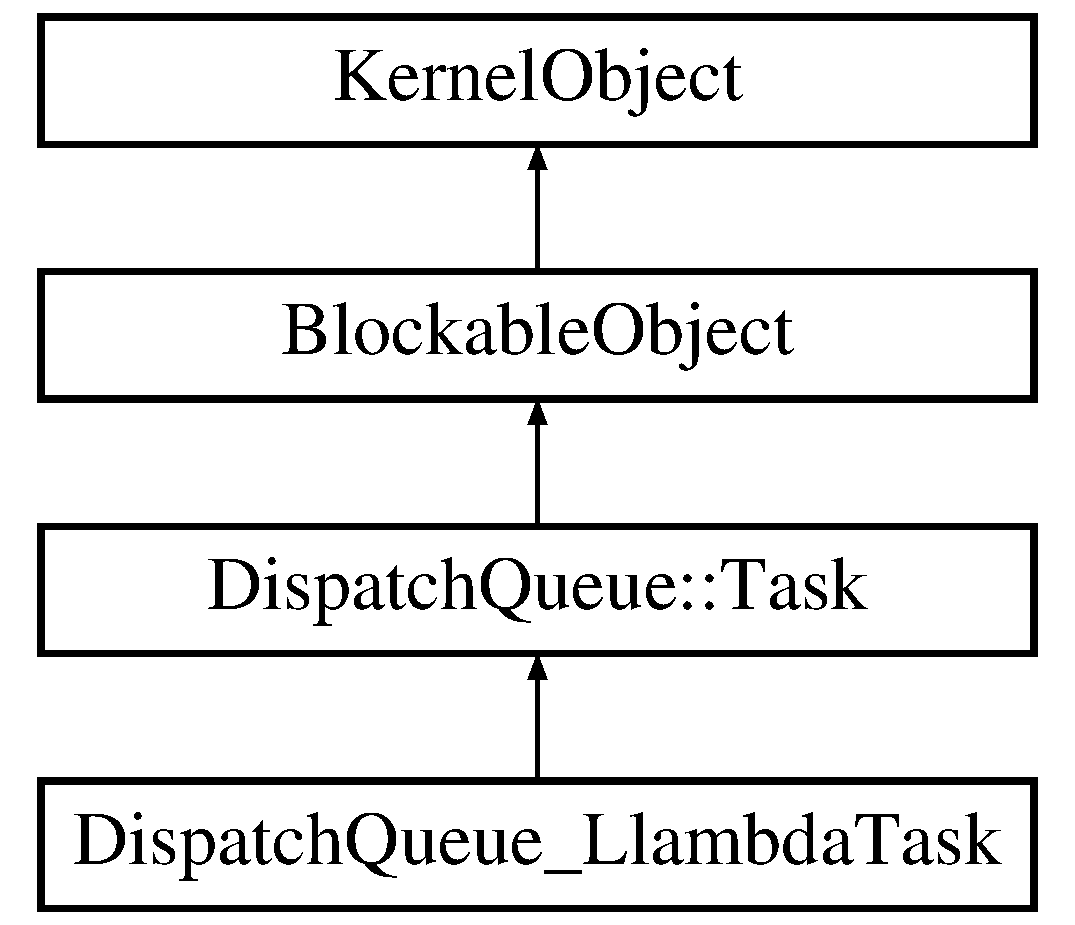
\includegraphics[height=4.000000cm]{class_dispatch_queue___llambda_task}
\end{center}
\end{figure}
\subsection*{Public Member Functions}
\begin{DoxyCompactItemize}
\item 
\mbox{\Hypertarget{class_dispatch_queue___llambda_task_a86b7f342ffba4b7ae41609ef5a31596f}\label{class_dispatch_queue___llambda_task_a86b7f342ffba4b7ae41609ef5a31596f}} 
const char $\ast$ {\bfseries Get\+Class\+Name} (U\+Int32 level)
\item 
\mbox{\Hypertarget{class_dispatch_queue___llambda_task_a7dc1f1f6c7a8608d175a2c511046a584}\label{class_dispatch_queue___llambda_task_a7dc1f1f6c7a8608d175a2c511046a584}} 
{\bfseries Dispatch\+Queue\+\_\+\+Llambda\+Task} (\hyperlink{classbicycle_1_1function}{bicycle\+::function}$<$ int(void)$>$ task)
\end{DoxyCompactItemize}
\subsection*{Protected Member Functions}
\begin{DoxyCompactItemize}
\item 
\mbox{\Hypertarget{class_dispatch_queue___llambda_task_a5bb5a09bf0b9b8613bb5cf91b2bc33b8}\label{class_dispatch_queue___llambda_task_a5bb5a09bf0b9b8613bb5cf91b2bc33b8}} 
void {\bfseries Execute} (void)
\end{DoxyCompactItemize}
\subsection*{Private Attributes}
\begin{DoxyCompactItemize}
\item 
\mbox{\Hypertarget{class_dispatch_queue___llambda_task_a32acee7d526ff77f7d1c3fc02d5bec0d}\label{class_dispatch_queue___llambda_task_a32acee7d526ff77f7d1c3fc02d5bec0d}} 
\hyperlink{classbicycle_1_1function}{bicycle\+::function}$<$ int(void)$>$ {\bfseries \+\_\+function}
\end{DoxyCompactItemize}
\subsection*{Additional Inherited Members}


The documentation for this class was generated from the following file\+:\begin{DoxyCompactItemize}
\item 
Queue.\+cpp\end{DoxyCompactItemize}

\hypertarget{class_d_m_a_buffer}{}\section{D\+M\+A\+Buffer Class Reference}
\label{class_d_m_a_buffer}\index{D\+M\+A\+Buffer@{D\+M\+A\+Buffer}}
\subsection*{Public Member Functions}
\begin{DoxyCompactItemize}
\item 
\mbox{\Hypertarget{class_d_m_a_buffer_a7b6e8fc6ef0e90e40567c8c31e19063a}\label{class_d_m_a_buffer_a7b6e8fc6ef0e90e40567c8c31e19063a}} 
Physical\+Pointer {\bfseries Physical} (void)
\item 
\mbox{\Hypertarget{class_d_m_a_buffer_ac179dd93f3efc0bc6a641d8187f200ff}\label{class_d_m_a_buffer_ac179dd93f3efc0bc6a641d8187f200ff}} 
void $\ast$ {\bfseries Virtual} (void)
\end{DoxyCompactItemize}
\subsection*{Private Attributes}
\begin{DoxyCompactItemize}
\item 
\mbox{\Hypertarget{class_d_m_a_buffer_a9a6610851e6fba3b913ece79813343b9}\label{class_d_m_a_buffer_a9a6610851e6fba3b913ece79813343b9}} 
Physical\+Pointer {\bfseries \+\_\+physical\+Address}
\item 
\mbox{\Hypertarget{class_d_m_a_buffer_ac292b7e9639bf901e49251e3f2b6bd3b}\label{class_d_m_a_buffer_ac292b7e9639bf901e49251e3f2b6bd3b}} 
void $\ast$ {\bfseries \+\_\+virtual\+Address}
\item 
\mbox{\Hypertarget{class_d_m_a_buffer_a136908f02c3bc48b27c188cf3a79cf19}\label{class_d_m_a_buffer_a136908f02c3bc48b27c188cf3a79cf19}} 
int {\bfseries \+\_\+allocated\+Pages}
\end{DoxyCompactItemize}


The documentation for this class was generated from the following file\+:\begin{DoxyCompactItemize}
\item 
Driver\+\_\+\+A\+T\+A.\+cpp\end{DoxyCompactItemize}

\hypertarget{class_driver}{}\section{Driver Class Reference}
\label{class_driver}\index{Driver@{Driver}}
Inheritance diagram for Driver\+:\begin{figure}[H]
\begin{center}
\leavevmode
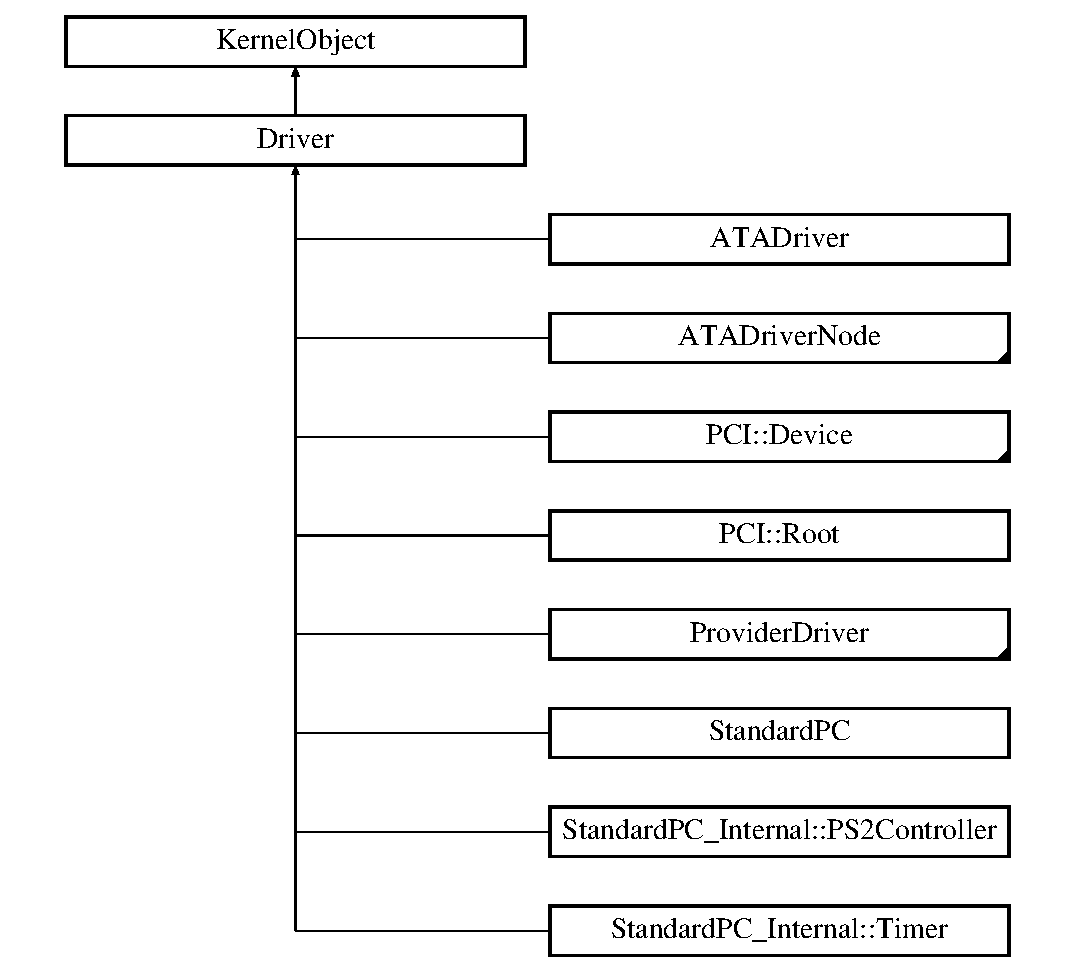
\includegraphics[height=10.000000cm]{class_driver}
\end{center}
\end{figure}
\subsection*{Public Member Functions}
\begin{DoxyCompactItemize}
\item 
\mbox{\Hypertarget{class_driver_a539239c6c0fa57667ae0997ef7da9d96}\label{class_driver_a539239c6c0fa57667ae0997ef7da9d96}} 
{\bfseries Driver} (const char $\ast$name)
\item 
\mbox{\Hypertarget{class_driver_a0b9ee00795cffded27141c950a8abbc2}\label{class_driver_a0b9ee00795cffded27141c950a8abbc2}} 
const char $\ast$ {\bfseries Get\+Class\+Name} (U\+Int32 level)
\item 
\mbox{\Hypertarget{class_driver_af3af210d6320609cbb81dd6368c6eacf}\label{class_driver_af3af210d6320609cbb81dd6368c6eacf}} 
virtual bool {\bfseries Start} (\hyperlink{class_driver}{Driver} $\ast$parent)
\item 
\mbox{\Hypertarget{class_driver_a6a4db5aaca6e3cdac7122b90b7abedb0}\label{class_driver_a6a4db5aaca6e3cdac7122b90b7abedb0}} 
virtual void {\bfseries Stop} (void)
\item 
\mbox{\Hypertarget{class_driver_a160ea51a9f3e9588f3a33bdc7f9c65a7}\label{class_driver_a160ea51a9f3e9588f3a33bdc7f9c65a7}} 
\hyperlink{class_driver}{Driver} $\ast$ {\bfseries Parent} (void)
\item 
\mbox{\Hypertarget{class_driver_a03f1c650a55570a51d79bfc1245084c2}\label{class_driver_a03f1c650a55570a51d79bfc1245084c2}} 
\hyperlink{class_driver}{Driver} $\ast$ {\bfseries Child} (int index)
\item 
\mbox{\Hypertarget{class_driver_a46822daa4eeba0a9da1acd786c95ca40}\label{class_driver_a46822daa4eeba0a9da1acd786c95ca40}} 
\hyperlink{class_interrupts}{Interrupts} $\ast$ {\bfseries Test} (void)
\item 
\mbox{\Hypertarget{class_driver_a53d7f2e9902a94c67515ba171b4b9943}\label{class_driver_a53d7f2e9902a94c67515ba171b4b9943}} 
\hyperlink{class_kernel_array}{Kernel\+Array} $\ast$ {\bfseries Property\+List} (void)
\item 
\mbox{\Hypertarget{class_driver_aa2977aba000e5ebdabf777295eba2618}\label{class_driver_aa2977aba000e5ebdabf777295eba2618}} 
\hyperlink{class_kernel_object}{Kernel\+Object} $\ast$ {\bfseries Property\+For} (\hyperlink{class_kernel_object}{Kernel\+Object} $\ast$property)
\item 
\mbox{\Hypertarget{class_driver_aca1cafa4d4695c093f5895d7d39be50d}\label{class_driver_aca1cafa4d4695c093f5895d7d39be50d}} 
virtual \hyperlink{class_interrupts}{Interrupts} $\ast$ {\bfseries Interrupt\+Source} (void)
\end{DoxyCompactItemize}
\subsection*{Static Public Member Functions}
\begin{DoxyCompactItemize}
\item 
\mbox{\Hypertarget{class_driver_ad97bd656791f23dd5ae7c3a8029d3b31}\label{class_driver_ad97bd656791f23dd5ae7c3a8029d3b31}} 
static void {\bfseries Configure\+Service} (void)
\item 
\mbox{\Hypertarget{class_driver_a4d57c158b21441adeeeeec3994674746}\label{class_driver_a4d57c158b21441adeeeeec3994674746}} 
static void {\bfseries Register\+Factory} (\hyperlink{class_driver_factory}{Driver\+Factory} $\ast$factory)
\item 
\mbox{\Hypertarget{class_driver_a3996984bc55f3c550b9a3d82673382e0}\label{class_driver_a3996984bc55f3c550b9a3d82673382e0}} 
static void {\bfseries Unregister\+Factory} (\hyperlink{class_driver_factory}{Driver\+Factory} $\ast$factory)
\end{DoxyCompactItemize}
\subsection*{Protected Member Functions}
\begin{DoxyCompactItemize}
\item 
\mbox{\Hypertarget{class_driver_a7688e9808028a867736f42aff745ba56}\label{class_driver_a7688e9808028a867736f42aff745ba56}} 
virtual bool {\bfseries Connect\+Child} (\hyperlink{class_driver}{Driver} $\ast$child)
\item 
\mbox{\Hypertarget{class_driver_a7d2bbb830c6059effcfe05cc6e2e0862}\label{class_driver_a7d2bbb830c6059effcfe05cc6e2e0862}} 
virtual void {\bfseries Detach\+Child} (\hyperlink{class_driver}{Driver} $\ast$child)
\item 
\mbox{\Hypertarget{class_driver_a12e96593446af8b1c55b972a2c3fa500}\label{class_driver_a12e96593446af8b1c55b972a2c3fa500}} 
void {\bfseries Set\+Property} (\hyperlink{class_kernel_object}{Kernel\+Object} $\ast$property, \hyperlink{class_kernel_object}{Kernel\+Object} $\ast$value)
\end{DoxyCompactItemize}
\subsection*{Private Attributes}
\begin{DoxyCompactItemize}
\item 
\mbox{\Hypertarget{class_driver_adbbee28d4b7694ead1ce602ff0e9cccd}\label{class_driver_adbbee28d4b7694ead1ce602ff0e9cccd}} 
\hyperlink{class_kernel_dictionary}{Kernel\+Dictionary} $\ast$ {\bfseries \+\_\+properties}
\item 
\mbox{\Hypertarget{class_driver_a1d4e0938f1466041e9a23ab6e7854f6f}\label{class_driver_a1d4e0938f1466041e9a23ab6e7854f6f}} 
\hyperlink{class_driver}{Driver} $\ast$ {\bfseries \+\_\+start}
\item 
\mbox{\Hypertarget{class_driver_a797564a13d3d85ecfc540e6669c19117}\label{class_driver_a797564a13d3d85ecfc540e6669c19117}} 
\hyperlink{class_driver}{Driver} $\ast$ {\bfseries \+\_\+end}
\item 
\mbox{\Hypertarget{class_driver_a1bebc8c02511a8fc6d69b54bc7880ed2}\label{class_driver_a1bebc8c02511a8fc6d69b54bc7880ed2}} 
\hyperlink{class_driver}{Driver} $\ast$ {\bfseries \+\_\+previous}
\item 
\mbox{\Hypertarget{class_driver_a10f419c14dea9d810246550a6da81e50}\label{class_driver_a10f419c14dea9d810246550a6da81e50}} 
\hyperlink{class_driver}{Driver} $\ast$ {\bfseries \+\_\+next}
\item 
\mbox{\Hypertarget{class_driver_ae3e26aff77965a463f52fd27f47eadf3}\label{class_driver_ae3e26aff77965a463f52fd27f47eadf3}} 
\hyperlink{class_driver}{Driver} $\ast$ {\bfseries \+\_\+parent}
\end{DoxyCompactItemize}


The documentation for this class was generated from the following files\+:\begin{DoxyCompactItemize}
\item 
Driver.\+h\item 
Driver.\+cpp\item 
System\+\_\+\+Service.\+cpp\end{DoxyCompactItemize}

\hypertarget{class_driver_factory}{}\section{Driver\+Factory Class Reference}
\label{class_driver_factory}\index{Driver\+Factory@{Driver\+Factory}}
Inheritance diagram for Driver\+Factory\+:\begin{figure}[H]
\begin{center}
\leavevmode
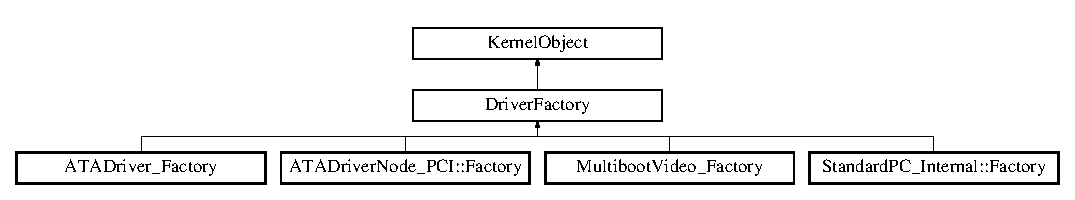
\includegraphics[height=2.234043cm]{class_driver_factory}
\end{center}
\end{figure}
\subsection*{Classes}
\begin{DoxyCompactItemize}
\item 
class \hyperlink{class_driver_factory_1_1_match}{Match}
\end{DoxyCompactItemize}
\subsection*{Public Member Functions}
\begin{DoxyCompactItemize}
\item 
\mbox{\Hypertarget{class_driver_factory_a5078ba6e7827958bb2ba233e4d3d2a2e}\label{class_driver_factory_a5078ba6e7827958bb2ba233e4d3d2a2e}} 
const char $\ast$ {\bfseries Get\+Class\+Name} (U\+Int32 level)
\item 
\mbox{\Hypertarget{class_driver_factory_ae714755a83d5e0a8ed20f156052e5b35}\label{class_driver_factory_ae714755a83d5e0a8ed20f156052e5b35}} 
virtual \hyperlink{class_kernel_array}{Kernel\+Array} $\ast$ {\bfseries Match\+For\+Parent} (\hyperlink{class_driver}{Driver} $\ast$parent)=0
\end{DoxyCompactItemize}
\subsection*{Additional Inherited Members}


The documentation for this class was generated from the following file\+:\begin{DoxyCompactItemize}
\item 
Driver.\+h\end{DoxyCompactItemize}

\hypertarget{class_d_r_q_handle__in_byte_rep}{}\section{D\+R\+Q\+Handle\+\_\+in\+Byte\+Rep Class Reference}
\label{class_d_r_q_handle__in_byte_rep}\index{D\+R\+Q\+Handle\+\_\+in\+Byte\+Rep@{D\+R\+Q\+Handle\+\_\+in\+Byte\+Rep}}
\subsection*{Static Public Member Functions}
\begin{DoxyCompactItemize}
\item 
\mbox{\Hypertarget{class_d_r_q_handle__in_byte_rep_aa7ff48a9c2278f27f3aa67e71e146ef7}\label{class_d_r_q_handle__in_byte_rep_aa7ff48a9c2278f27f3aa67e71e146ef7}} 
static void {\bfseries Handle} (\hyperlink{class_a_t_a_driver_node}{A\+T\+A\+Driver\+Node} $\ast$io, U\+Int8 reg, U\+Int8 $\ast$buffer, U\+Int32 length)
\end{DoxyCompactItemize}


The documentation for this class was generated from the following file\+:\begin{DoxyCompactItemize}
\item 
Driver\+\_\+\+A\+T\+A.\+cpp\end{DoxyCompactItemize}

\hypertarget{class_d_r_q_handle__in_long_rep}{}\section{D\+R\+Q\+Handle\+\_\+in\+Long\+Rep Class Reference}
\label{class_d_r_q_handle__in_long_rep}\index{D\+R\+Q\+Handle\+\_\+in\+Long\+Rep@{D\+R\+Q\+Handle\+\_\+in\+Long\+Rep}}
\subsection*{Static Public Member Functions}
\begin{DoxyCompactItemize}
\item 
\mbox{\Hypertarget{class_d_r_q_handle__in_long_rep_af51dff8cad08d8a2271c4144b52f4cb5}\label{class_d_r_q_handle__in_long_rep_af51dff8cad08d8a2271c4144b52f4cb5}} 
static void {\bfseries Handle} (\hyperlink{class_a_t_a_driver_node}{A\+T\+A\+Driver\+Node} $\ast$io, U\+Int8 reg, U\+Int8 $\ast$buffer, U\+Int32 length)
\end{DoxyCompactItemize}


The documentation for this class was generated from the following file\+:\begin{DoxyCompactItemize}
\item 
Driver\+\_\+\+A\+T\+A.\+cpp\end{DoxyCompactItemize}

\hypertarget{class_d_r_q_handle__in_short_rep}{}\section{D\+R\+Q\+Handle\+\_\+in\+Short\+Rep Class Reference}
\label{class_d_r_q_handle__in_short_rep}\index{D\+R\+Q\+Handle\+\_\+in\+Short\+Rep@{D\+R\+Q\+Handle\+\_\+in\+Short\+Rep}}
\subsection*{Static Public Member Functions}
\begin{DoxyCompactItemize}
\item 
\mbox{\Hypertarget{class_d_r_q_handle__in_short_rep_a551704e1c7b47db16b18ab840ee492fa}\label{class_d_r_q_handle__in_short_rep_a551704e1c7b47db16b18ab840ee492fa}} 
static void {\bfseries Handle} (\hyperlink{class_a_t_a_driver_node}{A\+T\+A\+Driver\+Node} $\ast$io, U\+Int8 reg, U\+Int8 $\ast$buffer, U\+Int32 length)
\end{DoxyCompactItemize}


The documentation for this class was generated from the following file\+:\begin{DoxyCompactItemize}
\item 
Driver\+\_\+\+A\+T\+A.\+cpp\end{DoxyCompactItemize}

\hypertarget{class_d_r_q_handle__out_byte_rep}{}\section{D\+R\+Q\+Handle\+\_\+out\+Byte\+Rep Class Reference}
\label{class_d_r_q_handle__out_byte_rep}\index{D\+R\+Q\+Handle\+\_\+out\+Byte\+Rep@{D\+R\+Q\+Handle\+\_\+out\+Byte\+Rep}}
\subsection*{Static Public Member Functions}
\begin{DoxyCompactItemize}
\item 
\mbox{\Hypertarget{class_d_r_q_handle__out_byte_rep_a5f9de061a65251dfd449821a957bfb9f}\label{class_d_r_q_handle__out_byte_rep_a5f9de061a65251dfd449821a957bfb9f}} 
static void {\bfseries Handle} (\hyperlink{class_a_t_a_driver_node}{A\+T\+A\+Driver\+Node} $\ast$io, U\+Int8 reg, U\+Int8 $\ast$buffer, U\+Int32 length)
\end{DoxyCompactItemize}


The documentation for this class was generated from the following file\+:\begin{DoxyCompactItemize}
\item 
Driver\+\_\+\+A\+T\+A.\+cpp\end{DoxyCompactItemize}

\hypertarget{class_d_r_q_handle__out_long_rep}{}\section{D\+R\+Q\+Handle\+\_\+out\+Long\+Rep Class Reference}
\label{class_d_r_q_handle__out_long_rep}\index{D\+R\+Q\+Handle\+\_\+out\+Long\+Rep@{D\+R\+Q\+Handle\+\_\+out\+Long\+Rep}}
\subsection*{Static Public Member Functions}
\begin{DoxyCompactItemize}
\item 
\mbox{\Hypertarget{class_d_r_q_handle__out_long_rep_acdc740d764873c7d6fc79bec1e76bf7f}\label{class_d_r_q_handle__out_long_rep_acdc740d764873c7d6fc79bec1e76bf7f}} 
static void {\bfseries Handle} (\hyperlink{class_a_t_a_driver_node}{A\+T\+A\+Driver\+Node} $\ast$io, U\+Int8 reg, U\+Int8 $\ast$buffer, U\+Int32 length)
\end{DoxyCompactItemize}


The documentation for this class was generated from the following file\+:\begin{DoxyCompactItemize}
\item 
Driver\+\_\+\+A\+T\+A.\+cpp\end{DoxyCompactItemize}

\hypertarget{class_d_r_q_handle__out_short_rep}{}\section{D\+R\+Q\+Handle\+\_\+out\+Short\+Rep Class Reference}
\label{class_d_r_q_handle__out_short_rep}\index{D\+R\+Q\+Handle\+\_\+out\+Short\+Rep@{D\+R\+Q\+Handle\+\_\+out\+Short\+Rep}}
\subsection*{Static Public Member Functions}
\begin{DoxyCompactItemize}
\item 
\mbox{\Hypertarget{class_d_r_q_handle__out_short_rep_adc99e4e4ee3a033aba2273923f705369}\label{class_d_r_q_handle__out_short_rep_adc99e4e4ee3a033aba2273923f705369}} 
static void {\bfseries Handle} (\hyperlink{class_a_t_a_driver_node}{A\+T\+A\+Driver\+Node} $\ast$io, U\+Int8 reg, U\+Int8 $\ast$buffer, U\+Int32 length)
\end{DoxyCompactItemize}


The documentation for this class was generated from the following file\+:\begin{DoxyCompactItemize}
\item 
Driver\+\_\+\+A\+T\+A.\+cpp\end{DoxyCompactItemize}

\hypertarget{struct_elf32___phdr}{}\section{Elf32\+\_\+\+Phdr Struct Reference}
\label{struct_elf32___phdr}\index{Elf32\+\_\+\+Phdr@{Elf32\+\_\+\+Phdr}}
\subsection*{Public Attributes}
\begin{DoxyCompactItemize}
\item 
\mbox{\Hypertarget{struct_elf32___phdr_a8b1d2942ddb9abcb85db1429b5116923}\label{struct_elf32___phdr_a8b1d2942ddb9abcb85db1429b5116923}} 
Elf32\+\_\+\+Word {\bfseries p\+\_\+type}
\item 
\mbox{\Hypertarget{struct_elf32___phdr_ac590d4c4b26104216e53058b5b03eef0}\label{struct_elf32___phdr_ac590d4c4b26104216e53058b5b03eef0}} 
Elf32\+\_\+\+Off {\bfseries p\+\_\+offset}
\item 
\mbox{\Hypertarget{struct_elf32___phdr_a01a298ebc899bcf9c23211a7bf1155a6}\label{struct_elf32___phdr_a01a298ebc899bcf9c23211a7bf1155a6}} 
Elf32\+\_\+\+Addr {\bfseries p\+\_\+vaddr}
\item 
\mbox{\Hypertarget{struct_elf32___phdr_af18f0a179a5fca09e3c04bcdce3fac2f}\label{struct_elf32___phdr_af18f0a179a5fca09e3c04bcdce3fac2f}} 
Elf32\+\_\+\+Addr {\bfseries p\+\_\+paddr}
\item 
\mbox{\Hypertarget{struct_elf32___phdr_ac9151f2e11001284bf1c7d2d2659555c}\label{struct_elf32___phdr_ac9151f2e11001284bf1c7d2d2659555c}} 
Elf32\+\_\+\+Word {\bfseries p\+\_\+filesz}
\item 
\mbox{\Hypertarget{struct_elf32___phdr_ada1cdd3d6ccb79a17bed0e3c21379c84}\label{struct_elf32___phdr_ada1cdd3d6ccb79a17bed0e3c21379c84}} 
Elf32\+\_\+\+Word {\bfseries p\+\_\+memsz}
\item 
\mbox{\Hypertarget{struct_elf32___phdr_a35c457e6828894b7b275730593802050}\label{struct_elf32___phdr_a35c457e6828894b7b275730593802050}} 
Elf32\+\_\+\+Word {\bfseries p\+\_\+flags}
\item 
\mbox{\Hypertarget{struct_elf32___phdr_afd09d9e4297b13fc94fd57d09f2a9f70}\label{struct_elf32___phdr_afd09d9e4297b13fc94fd57d09f2a9f70}} 
Elf32\+\_\+\+Word {\bfseries p\+\_\+align}
\end{DoxyCompactItemize}


The documentation for this struct was generated from the following file\+:\begin{DoxyCompactItemize}
\item 
elf.\+h\end{DoxyCompactItemize}

\hypertarget{class_elf_provider}{}\section{Elf\+Provider Class Reference}
\label{class_elf_provider}\index{Elf\+Provider@{Elf\+Provider}}
Inheritance diagram for Elf\+Provider\+:\begin{figure}[H]
\begin{center}
\leavevmode
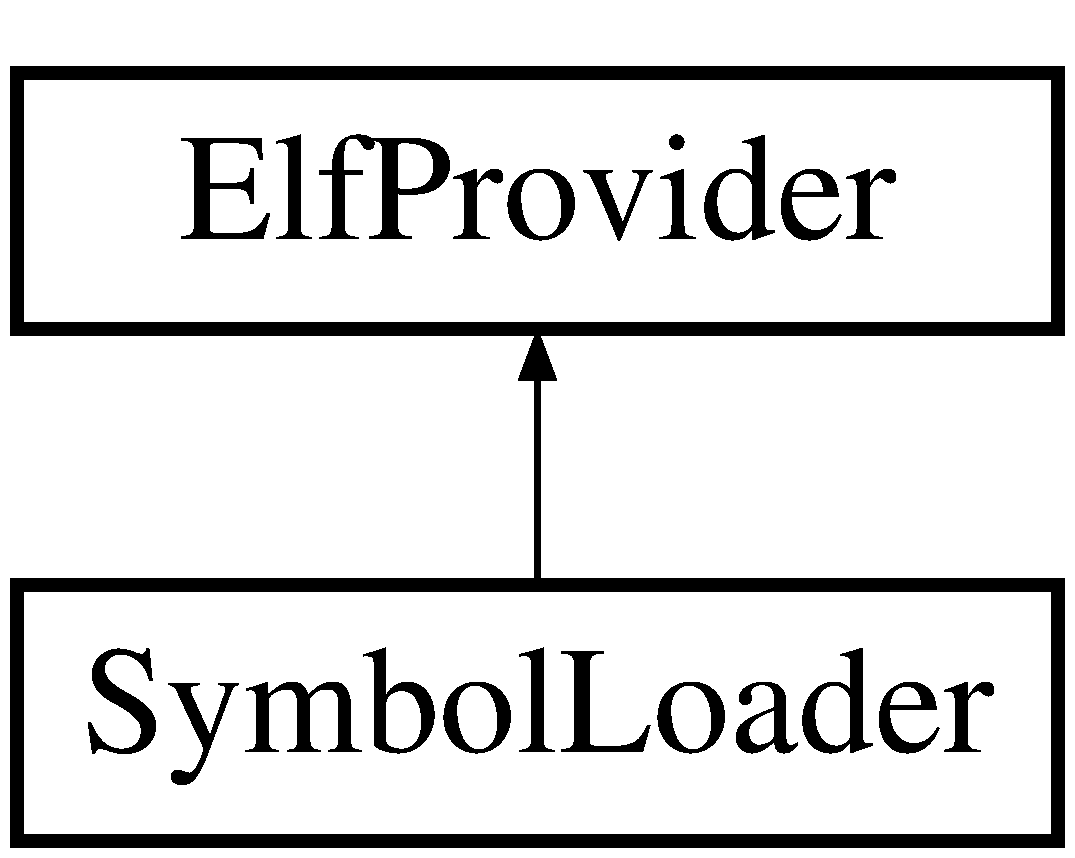
\includegraphics[height=2.000000cm]{class_elf_provider}
\end{center}
\end{figure}
\subsection*{Public Member Functions}
\begin{DoxyCompactItemize}
\item 
\mbox{\Hypertarget{class_elf_provider_ae757dbfaff68b095dee6685380c3ae8e}\label{class_elf_provider_ae757dbfaff68b095dee6685380c3ae8e}} 
virtual U\+Int64 {\bfseries Header} (void)=0
\item 
\mbox{\Hypertarget{class_elf_provider_a009de9ef2b4a261f7ef531950c165bc1}\label{class_elf_provider_a009de9ef2b4a261f7ef531950c165bc1}} 
virtual U\+Int64 {\bfseries Count} (void)=0
\item 
\mbox{\Hypertarget{class_elf_provider_a1aba51981b249d783ea9cb4a56839927}\label{class_elf_provider_a1aba51981b249d783ea9cb4a56839927}} 
virtual U\+Int64 {\bfseries Strndx} (void)=0
\item 
\mbox{\Hypertarget{class_elf_provider_ab92e6abc7309775a3f6bdd356928aeac}\label{class_elf_provider_ab92e6abc7309775a3f6bdd356928aeac}} 
virtual void $\ast$ {\bfseries Get\+Address} (U\+Int64 address)=0
\end{DoxyCompactItemize}


The documentation for this class was generated from the following file\+:\begin{DoxyCompactItemize}
\item 
elfsyms.\+h\end{DoxyCompactItemize}

\hypertarget{class_elf_symbols}{}\section{Elf\+Symbols Class Reference}
\label{class_elf_symbols}\index{Elf\+Symbols@{Elf\+Symbols}}
Inheritance diagram for Elf\+Symbols\+:\begin{figure}[H]
\begin{center}
\leavevmode
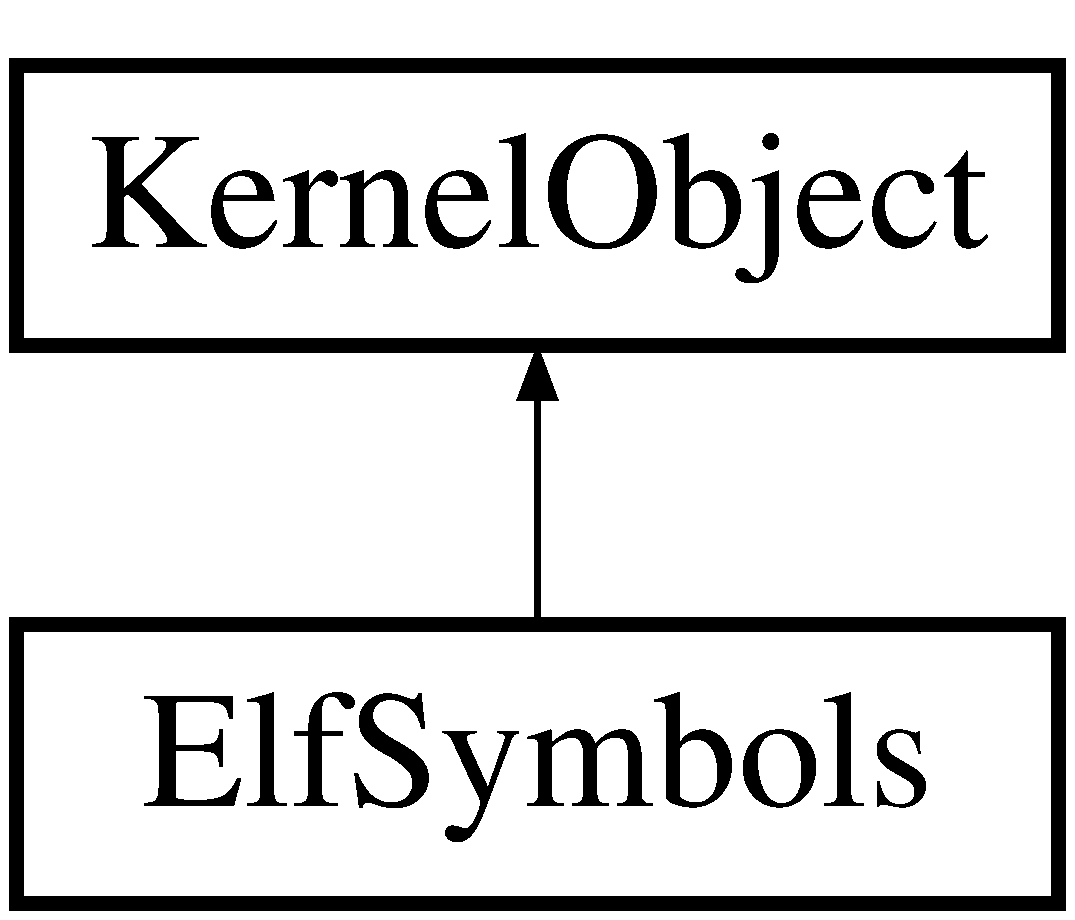
\includegraphics[height=2.000000cm]{class_elf_symbols}
\end{center}
\end{figure}
\subsection*{Classes}
\begin{DoxyCompactItemize}
\item 
class \hyperlink{class_elf_symbols_1_1_symbol}{Symbol}
\end{DoxyCompactItemize}
\subsection*{Public Member Functions}
\begin{DoxyCompactItemize}
\item 
\mbox{\Hypertarget{class_elf_symbols_ac304a4890081cb18f6cffe7a3384e54b}\label{class_elf_symbols_ac304a4890081cb18f6cffe7a3384e54b}} 
int {\bfseries Parse} (\hyperlink{class_elf_provider}{Elf\+Provider} $\ast$source)
\item 
\mbox{\Hypertarget{class_elf_symbols_a19cbe406d6752e860452252d72a97bb6}\label{class_elf_symbols_a19cbe406d6752e860452252d72a97bb6}} 
\hyperlink{class_elf_symbols_1_1_symbol}{Symbol} $\ast$ {\bfseries Find} (void $\ast$address)
\end{DoxyCompactItemize}
\subsection*{Private Attributes}
\begin{DoxyCompactItemize}
\item 
\mbox{\Hypertarget{class_elf_symbols_af33e568ee51c7020bf90dbf59d1e5807}\label{class_elf_symbols_af33e568ee51c7020bf90dbf59d1e5807}} 
\hyperlink{class_kernel_array}{Kernel\+Array} $\ast$ {\bfseries \+\_\+symbols}
\end{DoxyCompactItemize}
\subsection*{Additional Inherited Members}


The documentation for this class was generated from the following files\+:\begin{DoxyCompactItemize}
\item 
elfsyms.\+h\item 
elfsyms.\+cpp\end{DoxyCompactItemize}

\hypertarget{class_entry}{}\section{Entry Class Reference}
\label{class_entry}\index{Entry@{Entry}}
\subsection*{Public Member Functions}
\begin{DoxyCompactItemize}
\item 
\mbox{\Hypertarget{class_entry_a0b21b906d47583a54d4676495ea85012}\label{class_entry_a0b21b906d47583a54d4676495ea85012}} 
{\bfseries Entry} (\hyperlink{class_entry}{Entry} $\ast$$\ast$start, \hyperlink{class_entry}{Entry} $\ast$$\ast$end, \hyperlink{class_kernel_object}{Kernel\+Object} $\ast$key, \hyperlink{class_kernel_object}{Kernel\+Object} $\ast$value)
\item 
\mbox{\Hypertarget{class_entry_ad81b59692d342f8f8de06f46a3921e91}\label{class_entry_ad81b59692d342f8f8de06f46a3921e91}} 
void {\bfseries Change} (\hyperlink{class_kernel_object}{Kernel\+Object} $\ast$value)
\end{DoxyCompactItemize}
\subsection*{Public Attributes}
\begin{DoxyCompactItemize}
\item 
\mbox{\Hypertarget{class_entry_a56be933167cac18b9c5591a41d180739}\label{class_entry_a56be933167cac18b9c5591a41d180739}} 
\hyperlink{class_kernel_object}{Kernel\+Object} $\ast$ {\bfseries key}
\item 
\mbox{\Hypertarget{class_entry_a66559cc407bee32b494006d4014aa9af}\label{class_entry_a66559cc407bee32b494006d4014aa9af}} 
\hyperlink{class_kernel_object}{Kernel\+Object} $\ast$ {\bfseries value}
\item 
\mbox{\Hypertarget{class_entry_ac2f98827296edee00ac27ea720a0e619}\label{class_entry_ac2f98827296edee00ac27ea720a0e619}} 
\hyperlink{class_entry}{Entry} $\ast$ {\bfseries \+\_\+next}
\end{DoxyCompactItemize}
\subsection*{Private Attributes}
\begin{DoxyCompactItemize}
\item 
\mbox{\Hypertarget{class_entry_a499af520da687360af294e2fdd51367c}\label{class_entry_a499af520da687360af294e2fdd51367c}} 
\hyperlink{class_entry}{Entry} $\ast$$\ast$ {\bfseries \+\_\+start}
\item 
\mbox{\Hypertarget{class_entry_af041afc13e5ffe93bab70a0afe3960db}\label{class_entry_af041afc13e5ffe93bab70a0afe3960db}} 
\hyperlink{class_entry}{Entry} $\ast$$\ast$ {\bfseries \+\_\+end}
\item 
\mbox{\Hypertarget{class_entry_a7a59c156aea6cff3e427df87479b2610}\label{class_entry_a7a59c156aea6cff3e427df87479b2610}} 
\hyperlink{class_entry}{Entry} $\ast$ {\bfseries \+\_\+previous}
\end{DoxyCompactItemize}


The documentation for this class was generated from the following file\+:\begin{DoxyCompactItemize}
\item 
Collections.\+cpp\end{DoxyCompactItemize}

\hypertarget{class_i_p_c___manager___internal_1_1_entry}{}\section{I\+P\+C\+\_\+\+Manager\+\_\+\+Internal\+:\+:Entry Class Reference}
\label{class_i_p_c___manager___internal_1_1_entry}\index{I\+P\+C\+\_\+\+Manager\+\_\+\+Internal\+::\+Entry@{I\+P\+C\+\_\+\+Manager\+\_\+\+Internal\+::\+Entry}}
\subsection*{Public Types}
\begin{DoxyCompactItemize}
\item 
\mbox{\Hypertarget{class_i_p_c___manager___internal_1_1_entry_a94f0b89803d1929ab5c2b5eb2f1afb9c}\label{class_i_p_c___manager___internal_1_1_entry_a94f0b89803d1929ab5c2b5eb2f1afb9c}} 
enum {\bfseries Type} \{ \newline
{\bfseries type\+Invalid} = 0, 
{\bfseries type\+Provider} = 1 $<$$<$ 1, 
{\bfseries type\+Input} = 1 $<$$<$ 2, 
{\bfseries type\+Output} = 1 $<$$<$ 3, 
\newline
{\bfseries type\+Input\+Connection} = 1 $<$$<$ 4, 
{\bfseries type\+Output\+Connection} = 1 $<$$<$ 5, 
{\bfseries type\+Start} = 0, 
{\bfseries type\+Stop} = 1
 \}
\end{DoxyCompactItemize}
\subsection*{Public Member Functions}
\begin{DoxyCompactItemize}
\item 
\mbox{\Hypertarget{class_i_p_c___manager___internal_1_1_entry_a2ff426f22a51d430862f6cabf85e2a45}\label{class_i_p_c___manager___internal_1_1_entry_a2ff426f22a51d430862f6cabf85e2a45}} 
{\bfseries Entry} (\hyperlink{class_i_p_c___manager___internal_1_1_entry}{Entry} $\ast$$\ast$start, \hyperlink{class_i_p_c___manager___internal_1_1_entry}{Entry} $\ast$$\ast$end, U\+Int32 provider, U\+Int32 io\+Port, U\+Int32 connection, Type type)
\item 
\mbox{\Hypertarget{class_i_p_c___manager___internal_1_1_entry_ae9f73fa712c307cf434237bc2d05969a}\label{class_i_p_c___manager___internal_1_1_entry_ae9f73fa712c307cf434237bc2d05969a}} 
int {\bfseries Cancel\+If\+Necessary} (void)
\item 
\mbox{\Hypertarget{class_i_p_c___manager___internal_1_1_entry_a7615fe5e9643d8548448c477e30a3f3f}\label{class_i_p_c___manager___internal_1_1_entry_a7615fe5e9643d8548448c477e30a3f3f}} 
\hyperlink{class_kernel_dictionary}{Kernel\+Dictionary} $\ast$ {\bfseries Get\+Info} (void)
\end{DoxyCompactItemize}
\subsection*{Static Public Member Functions}
\begin{DoxyCompactItemize}
\item 
\mbox{\Hypertarget{class_i_p_c___manager___internal_1_1_entry_ac0139be73bef62997dff89d613914088}\label{class_i_p_c___manager___internal_1_1_entry_ac0139be73bef62997dff89d613914088}} 
static U\+Int32 {\bfseries Map} (\hyperlink{class_kernel_object}{Kernel\+Object} $\ast$object)
\item 
\mbox{\Hypertarget{class_i_p_c___manager___internal_1_1_entry_ab93847831a98c8904b96e18bf27ed16d}\label{class_i_p_c___manager___internal_1_1_entry_ab93847831a98c8904b96e18bf27ed16d}} 
static \hyperlink{class_kernel_object}{Kernel\+Object} $\ast$ {\bfseries Demap} (U\+Int32 map)
\end{DoxyCompactItemize}
\subsection*{Public Attributes}
\begin{DoxyCompactItemize}
\item 
\mbox{\Hypertarget{class_i_p_c___manager___internal_1_1_entry_a95a5e38367ca5053d8a930a1888a1de7}\label{class_i_p_c___manager___internal_1_1_entry_a95a5e38367ca5053d8a930a1888a1de7}} 
Type {\bfseries \+\_\+type}
\item 
\mbox{\Hypertarget{class_i_p_c___manager___internal_1_1_entry_ae0b5352d87361aef2b21bdf42875115c}\label{class_i_p_c___manager___internal_1_1_entry_ae0b5352d87361aef2b21bdf42875115c}} 
U\+Int32 {\bfseries \+\_\+provider\+Handle}
\item 
\mbox{\Hypertarget{class_i_p_c___manager___internal_1_1_entry_a767b725f2fccfc545e1639cd271fd3b5}\label{class_i_p_c___manager___internal_1_1_entry_a767b725f2fccfc545e1639cd271fd3b5}} 
U\+Int32 {\bfseries \+\_\+io\+Handle}
\item 
\mbox{\Hypertarget{class_i_p_c___manager___internal_1_1_entry_a57021dc9a582b3b5df8725e949601645}\label{class_i_p_c___manager___internal_1_1_entry_a57021dc9a582b3b5df8725e949601645}} 
U\+Int32 {\bfseries \+\_\+connection\+Handle}
\item 
\mbox{\Hypertarget{class_i_p_c___manager___internal_1_1_entry_a8f69bdd17278046052028180cfa1fc10}\label{class_i_p_c___manager___internal_1_1_entry_a8f69bdd17278046052028180cfa1fc10}} 
\hyperlink{class_i_p_c___manager___internal_1_1_entry}{Entry} $\ast$$\ast$ {\bfseries \+\_\+start}
\item 
\mbox{\Hypertarget{class_i_p_c___manager___internal_1_1_entry_aabeb2cf3d6d04febddcfc8d0ce360ee2}\label{class_i_p_c___manager___internal_1_1_entry_aabeb2cf3d6d04febddcfc8d0ce360ee2}} 
\hyperlink{class_i_p_c___manager___internal_1_1_entry}{Entry} $\ast$$\ast$ {\bfseries \+\_\+end}
\item 
\mbox{\Hypertarget{class_i_p_c___manager___internal_1_1_entry_ab547daa6dd7418717f894413b14408d8}\label{class_i_p_c___manager___internal_1_1_entry_ab547daa6dd7418717f894413b14408d8}} 
\hyperlink{class_i_p_c___manager___internal_1_1_entry}{Entry} $\ast$ {\bfseries \+\_\+last}
\item 
\mbox{\Hypertarget{class_i_p_c___manager___internal_1_1_entry_a16615d2ccd3623477dbb659fe0a1a366}\label{class_i_p_c___manager___internal_1_1_entry_a16615d2ccd3623477dbb659fe0a1a366}} 
\hyperlink{class_i_p_c___manager___internal_1_1_entry}{Entry} $\ast$ {\bfseries \+\_\+next}
\end{DoxyCompactItemize}
\subsection*{Static Private Member Functions}
\begin{DoxyCompactItemize}
\item 
\mbox{\Hypertarget{class_i_p_c___manager___internal_1_1_entry_ac72cd2f47ac111bba36fd03cbecee9b6}\label{class_i_p_c___manager___internal_1_1_entry_ac72cd2f47ac111bba36fd03cbecee9b6}} 
static \hyperlink{class_kernel_number}{Kernel\+Number} $\ast$ {\bfseries Number} (U\+Int32 handle)
\item 
\mbox{\Hypertarget{class_i_p_c___manager___internal_1_1_entry_a28d84c1ef0d3cdd6d30183fe9d3f6766}\label{class_i_p_c___manager___internal_1_1_entry_a28d84c1ef0d3cdd6d30183fe9d3f6766}} 
static \hyperlink{class_kernel_string}{Kernel\+String} $\ast$ {\bfseries State} (Type type)
\item 
\mbox{\Hypertarget{class_i_p_c___manager___internal_1_1_entry_a0f2be2d7dd6403bdac2a8a2a5483bdc2}\label{class_i_p_c___manager___internal_1_1_entry_a0f2be2d7dd6403bdac2a8a2a5483bdc2}} 
static \hyperlink{class_kernel_string}{Kernel\+String} $\ast$ {\bfseries Type\+Name} (Type type)
\end{DoxyCompactItemize}


The documentation for this class was generated from the following file\+:\begin{DoxyCompactItemize}
\item 
I\+P\+C\+\_\+\+Manager.\+cpp\end{DoxyCompactItemize}

\hypertarget{class_generic_provider_1_1_factory}{}\section{Generic\+Provider\+:\+:Factory Class Reference}
\label{class_generic_provider_1_1_factory}\index{Generic\+Provider\+::\+Factory@{Generic\+Provider\+::\+Factory}}
Inheritance diagram for Generic\+Provider\+:\+:Factory\+:\begin{figure}[H]
\begin{center}
\leavevmode
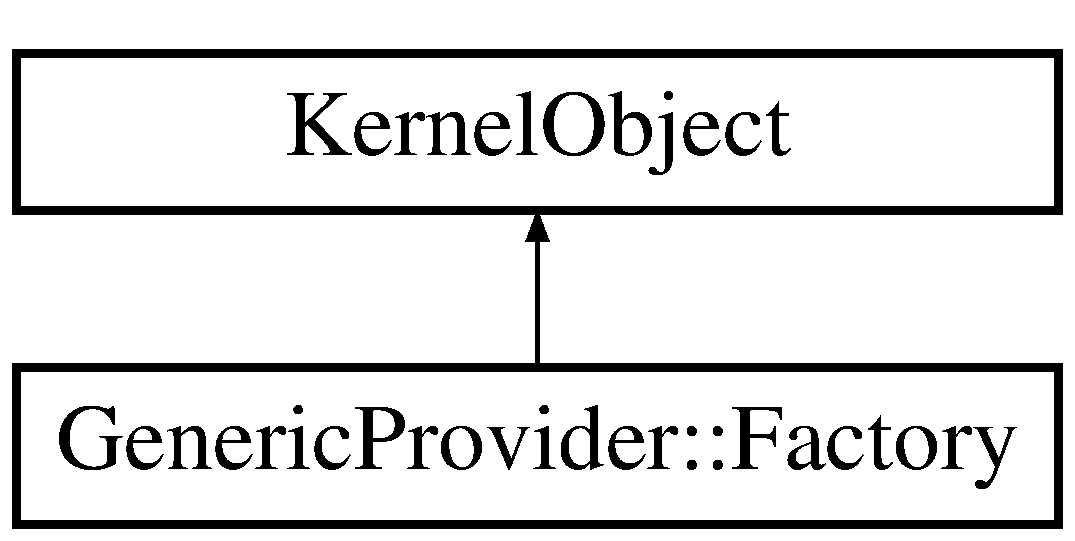
\includegraphics[height=2.000000cm]{class_generic_provider_1_1_factory}
\end{center}
\end{figure}
\subsection*{Public Member Functions}
\begin{DoxyCompactItemize}
\item 
\mbox{\Hypertarget{class_generic_provider_1_1_factory_a14f7b9bfd314c51a15425e64e871e4ba}\label{class_generic_provider_1_1_factory_a14f7b9bfd314c51a15425e64e871e4ba}} 
const char $\ast$ {\bfseries Get\+Class\+Name} (U\+Int32 level)
\item 
\mbox{\Hypertarget{class_generic_provider_1_1_factory_a4e5419dabf227fef04089557787efefd}\label{class_generic_provider_1_1_factory_a4e5419dabf227fef04089557787efefd}} 
virtual \hyperlink{class_kernel_dictionary}{Kernel\+Dictionary} $\ast$ {\bfseries Information} (void)=0
\item 
\mbox{\Hypertarget{class_generic_provider_1_1_factory_a8358aa2ab2b2d09c791d1a57ae039be1}\label{class_generic_provider_1_1_factory_a8358aa2ab2b2d09c791d1a57ae039be1}} 
virtual U\+Int32 {\bfseries Expected\+Input} (void)=0
\item 
\mbox{\Hypertarget{class_generic_provider_1_1_factory_ad0c495bd0326c020a569090aa28d2863}\label{class_generic_provider_1_1_factory_ad0c495bd0326c020a569090aa28d2863}} 
virtual \hyperlink{class_kernel_dictionary}{Kernel\+Dictionary} $\ast$ {\bfseries Expected\+Input\+Info} (U\+Int32 index)=0
\item 
\mbox{\Hypertarget{class_generic_provider_1_1_factory_af27e5ddd34bf68d5b21cfa45c2feef51}\label{class_generic_provider_1_1_factory_af27e5ddd34bf68d5b21cfa45c2feef51}} 
virtual U\+Int32 {\bfseries Expected\+Output} (void)=0
\item 
\mbox{\Hypertarget{class_generic_provider_1_1_factory_a493dc19e38e1d2529536bfb662f96d4f}\label{class_generic_provider_1_1_factory_a493dc19e38e1d2529536bfb662f96d4f}} 
virtual \hyperlink{class_kernel_dictionary}{Kernel\+Dictionary} $\ast$ {\bfseries Expected\+Output\+Info} (U\+Int32 index)=0
\item 
\mbox{\Hypertarget{class_generic_provider_1_1_factory_a7e7fac279e81b7a0d1db7a33ab7c4a1a}\label{class_generic_provider_1_1_factory_a7e7fac279e81b7a0d1db7a33ab7c4a1a}} 
virtual \hyperlink{class_generic_provider}{Generic\+Provider} $\ast$ {\bfseries Create} (void)=0
\end{DoxyCompactItemize}
\subsection*{Additional Inherited Members}


The documentation for this class was generated from the following file\+:\begin{DoxyCompactItemize}
\item 
Provider.\+h\end{DoxyCompactItemize}

\hypertarget{class_standard_p_c___internal_1_1_factory}{}\section{Standard\+P\+C\+\_\+\+Internal\+:\+:Factory Class Reference}
\label{class_standard_p_c___internal_1_1_factory}\index{Standard\+P\+C\+\_\+\+Internal\+::\+Factory@{Standard\+P\+C\+\_\+\+Internal\+::\+Factory}}
Inheritance diagram for Standard\+P\+C\+\_\+\+Internal\+:\+:Factory\+:\begin{figure}[H]
\begin{center}
\leavevmode
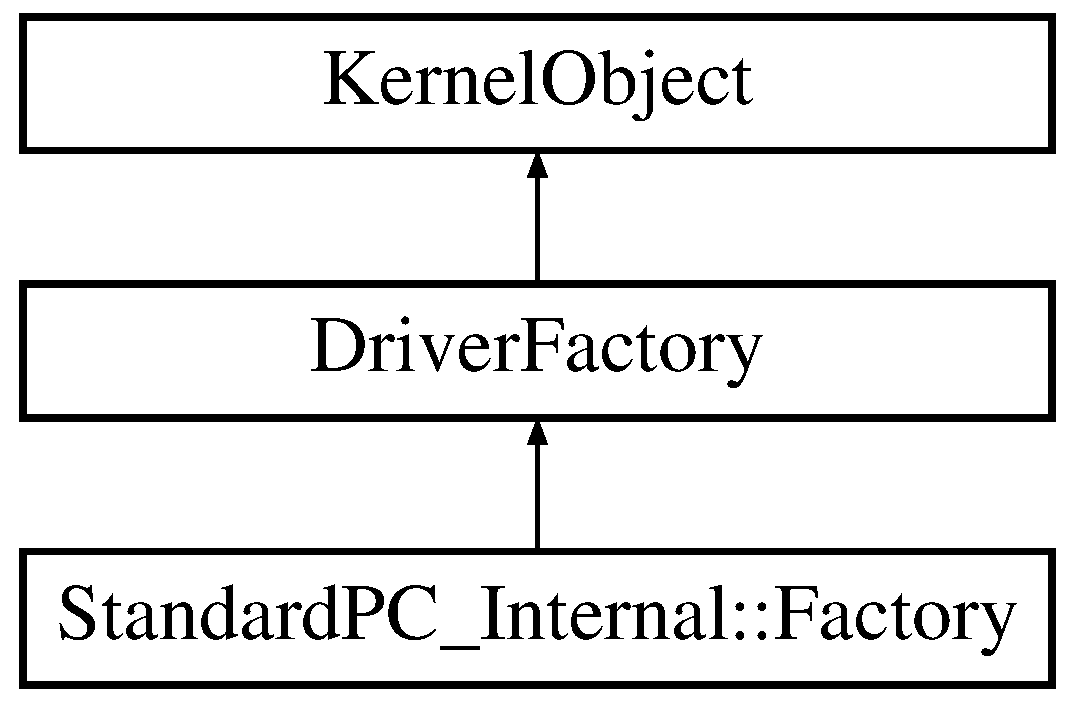
\includegraphics[height=3.000000cm]{class_standard_p_c___internal_1_1_factory}
\end{center}
\end{figure}
\subsection*{Classes}
\begin{DoxyCompactItemize}
\item 
class \hyperlink{class_standard_p_c___internal_1_1_factory_1_1_match___i_d_e}{Match\+\_\+\+I\+DE}
\item 
class \hyperlink{class_standard_p_c___internal_1_1_factory_1_1_match___keyboard}{Match\+\_\+\+Keyboard}
\item 
class \hyperlink{class_standard_p_c___internal_1_1_factory_1_1_match___p_c_i}{Match\+\_\+\+P\+CI}
\item 
class \hyperlink{class_standard_p_c___internal_1_1_factory_1_1_match___timer}{Match\+\_\+\+Timer}
\end{DoxyCompactItemize}
\subsection*{Public Member Functions}
\begin{DoxyCompactItemize}
\item 
\mbox{\Hypertarget{class_standard_p_c___internal_1_1_factory_a6f08529f24ebbfd458212eaad303b6d1}\label{class_standard_p_c___internal_1_1_factory_a6f08529f24ebbfd458212eaad303b6d1}} 
const char $\ast$ {\bfseries Get\+Class\+Name} (U\+Int32 level)
\item 
\mbox{\Hypertarget{class_standard_p_c___internal_1_1_factory_abf4d5bb16337cf994540d8923e87e2ce}\label{class_standard_p_c___internal_1_1_factory_abf4d5bb16337cf994540d8923e87e2ce}} 
\hyperlink{class_kernel_array}{Kernel\+Array} $\ast$ {\bfseries Match\+For\+Parent} (\hyperlink{class_driver}{Driver} $\ast$parent)
\end{DoxyCompactItemize}
\subsection*{Static Public Member Functions}
\begin{DoxyCompactItemize}
\item 
\mbox{\Hypertarget{class_standard_p_c___internal_1_1_factory_aee622428354b75acb132461d7016758d}\label{class_standard_p_c___internal_1_1_factory_aee622428354b75acb132461d7016758d}} 
static void {\bfseries Install} (void)
\end{DoxyCompactItemize}


The documentation for this class was generated from the following file\+:\begin{DoxyCompactItemize}
\item 
Standard\+P\+C.\+cpp\end{DoxyCompactItemize}

\hypertarget{class_a_t_a_driver_node___p_c_i_1_1_factory}{}\section{A\+T\+A\+Driver\+Node\+\_\+\+P\+CI\+:\+:Factory Class Reference}
\label{class_a_t_a_driver_node___p_c_i_1_1_factory}\index{A\+T\+A\+Driver\+Node\+\_\+\+P\+C\+I\+::\+Factory@{A\+T\+A\+Driver\+Node\+\_\+\+P\+C\+I\+::\+Factory}}
Inheritance diagram for A\+T\+A\+Driver\+Node\+\_\+\+P\+CI\+:\+:Factory\+:\begin{figure}[H]
\begin{center}
\leavevmode
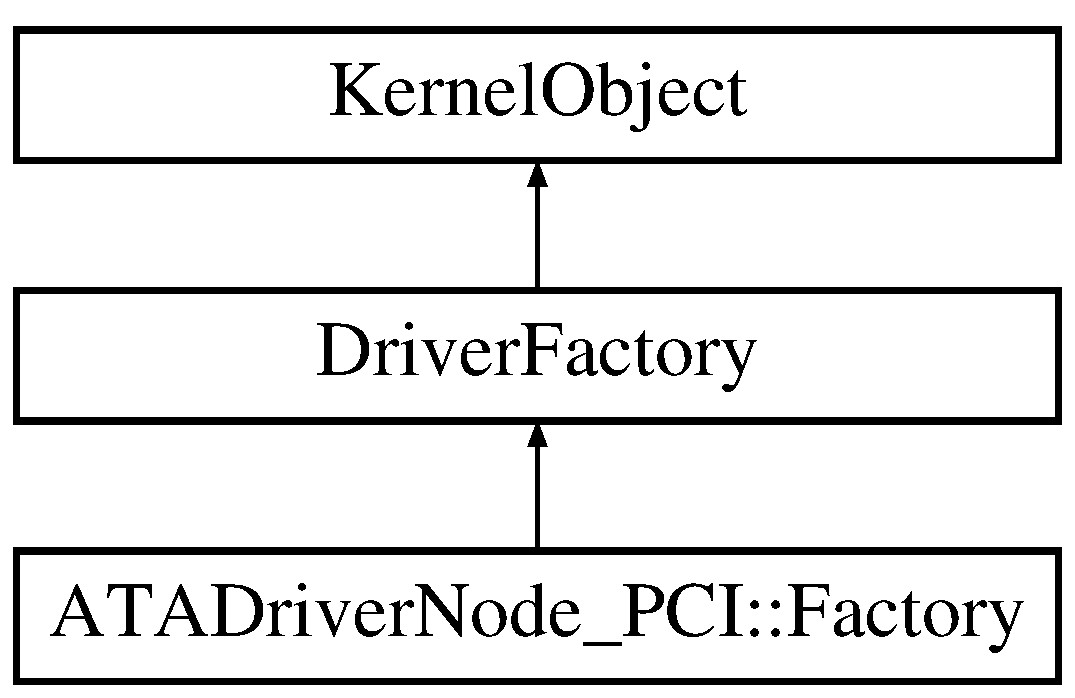
\includegraphics[height=3.000000cm]{class_a_t_a_driver_node___p_c_i_1_1_factory}
\end{center}
\end{figure}
\subsection*{Classes}
\begin{DoxyCompactItemize}
\item 
class \hyperlink{class_a_t_a_driver_node___p_c_i_1_1_factory_1_1_match}{Match}
\end{DoxyCompactItemize}
\subsection*{Public Member Functions}
\begin{DoxyCompactItemize}
\item 
\mbox{\Hypertarget{class_a_t_a_driver_node___p_c_i_1_1_factory_abec01459a9aa821e1e1ba3a1716c035f}\label{class_a_t_a_driver_node___p_c_i_1_1_factory_abec01459a9aa821e1e1ba3a1716c035f}} 
const char $\ast$ {\bfseries Get\+Class\+Name} (U\+Int32 level)
\item 
\mbox{\Hypertarget{class_a_t_a_driver_node___p_c_i_1_1_factory_aabb222d09a3fb9884208c4de48dd5f39}\label{class_a_t_a_driver_node___p_c_i_1_1_factory_aabb222d09a3fb9884208c4de48dd5f39}} 
\hyperlink{class_kernel_array}{Kernel\+Array} $\ast$ {\bfseries Match\+For\+Parent} (\hyperlink{class_driver}{Driver} $\ast$parent)
\end{DoxyCompactItemize}
\subsection*{Additional Inherited Members}


The documentation for this class was generated from the following file\+:\begin{DoxyCompactItemize}
\item 
Driver\+\_\+\+A\+T\+A.\+cpp\end{DoxyCompactItemize}

\hypertarget{class_f_i_f_o_item}{}\section{F\+I\+F\+O\+Item Class Reference}
\label{class_f_i_f_o_item}\index{F\+I\+F\+O\+Item@{F\+I\+F\+O\+Item}}
\subsection*{Public Member Functions}
\begin{DoxyCompactItemize}
\item 
\mbox{\Hypertarget{class_f_i_f_o_item_a7650d9cf486522770f8092db4e723dd6}\label{class_f_i_f_o_item_a7650d9cf486522770f8092db4e723dd6}} 
{\bfseries F\+I\+F\+O\+Item} (\hyperlink{class_f_i_f_o_item}{F\+I\+F\+O\+Item} $\ast$$\ast$start, \hyperlink{class_f_i_f_o_item}{F\+I\+F\+O\+Item} $\ast$$\ast$end, \hyperlink{class_kernel_object}{Kernel\+Object} $\ast$item)
\end{DoxyCompactItemize}
\subsection*{Public Attributes}
\begin{DoxyCompactItemize}
\item 
\mbox{\Hypertarget{class_f_i_f_o_item_af8be2d98e69407c5a4d9c004edd79629}\label{class_f_i_f_o_item_af8be2d98e69407c5a4d9c004edd79629}} 
\hyperlink{class_kernel_object}{Kernel\+Object} $\ast$ {\bfseries item}
\end{DoxyCompactItemize}
\subsection*{Private Attributes}
\begin{DoxyCompactItemize}
\item 
\mbox{\Hypertarget{class_f_i_f_o_item_a7a682c43d321c8190b719f712bfb5033}\label{class_f_i_f_o_item_a7a682c43d321c8190b719f712bfb5033}} 
\hyperlink{class_f_i_f_o_item}{F\+I\+F\+O\+Item} $\ast$$\ast$ {\bfseries \+\_\+start}
\item 
\mbox{\Hypertarget{class_f_i_f_o_item_a604e993a66c03b8bb92aeb9a38119605}\label{class_f_i_f_o_item_a604e993a66c03b8bb92aeb9a38119605}} 
\hyperlink{class_f_i_f_o_item}{F\+I\+F\+O\+Item} $\ast$$\ast$ {\bfseries \+\_\+end}
\item 
\mbox{\Hypertarget{class_f_i_f_o_item_a88962d8827231a34a58091315a7885ed}\label{class_f_i_f_o_item_a88962d8827231a34a58091315a7885ed}} 
\hyperlink{class_f_i_f_o_item}{F\+I\+F\+O\+Item} $\ast$ {\bfseries \+\_\+previous}
\item 
\mbox{\Hypertarget{class_f_i_f_o_item_a79213d288c782ab14af33519198c4e44}\label{class_f_i_f_o_item_a79213d288c782ab14af33519198c4e44}} 
\hyperlink{class_f_i_f_o_item}{F\+I\+F\+O\+Item} $\ast$ {\bfseries \+\_\+next}
\end{DoxyCompactItemize}


The documentation for this class was generated from the following file\+:\begin{DoxyCompactItemize}
\item 
Collections.\+cpp\end{DoxyCompactItemize}

\hypertarget{class_i_s_o9660_driver_1_1_file_entry}{}\section{I\+S\+O9660\+Driver\+:\+:File\+Entry Class Reference}
\label{class_i_s_o9660_driver_1_1_file_entry}\index{I\+S\+O9660\+Driver\+::\+File\+Entry@{I\+S\+O9660\+Driver\+::\+File\+Entry}}
Inheritance diagram for I\+S\+O9660\+Driver\+:\+:File\+Entry\+:\begin{figure}[H]
\begin{center}
\leavevmode
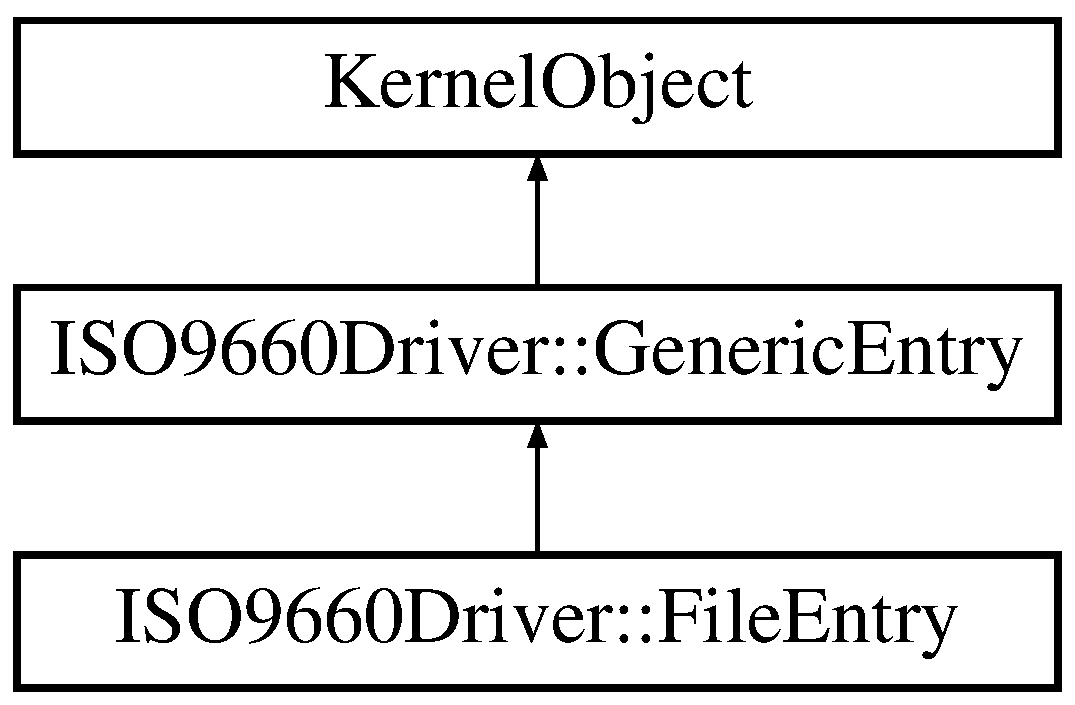
\includegraphics[height=3.000000cm]{class_i_s_o9660_driver_1_1_file_entry}
\end{center}
\end{figure}
\subsection*{Public Member Functions}
\begin{DoxyCompactItemize}
\item 
\mbox{\Hypertarget{class_i_s_o9660_driver_1_1_file_entry_a15e1b9456428da2c1fe3e3ba676ee9b8}\label{class_i_s_o9660_driver_1_1_file_entry_a15e1b9456428da2c1fe3e3ba676ee9b8}} 
const char $\ast$ {\bfseries Get\+Class\+Name} (U\+Int32 level)
\item 
\mbox{\Hypertarget{class_i_s_o9660_driver_1_1_file_entry_af19d975ca0424aef0085091fe6ab9fad}\label{class_i_s_o9660_driver_1_1_file_entry_af19d975ca0424aef0085091fe6ab9fad}} 
{\bfseries File\+Entry} (Directory\+Record $\ast$record)
\end{DoxyCompactItemize}
\subsection*{Additional Inherited Members}


The documentation for this class was generated from the following file\+:\begin{DoxyCompactItemize}
\item 
fs\+\_\+iso9660.\+cpp\end{DoxyCompactItemize}

\hypertarget{class_file_nubbin}{}\section{File\+Nubbin Class Reference}
\label{class_file_nubbin}\index{File\+Nubbin@{File\+Nubbin}}
Inheritance diagram for File\+Nubbin\+:\begin{figure}[H]
\begin{center}
\leavevmode
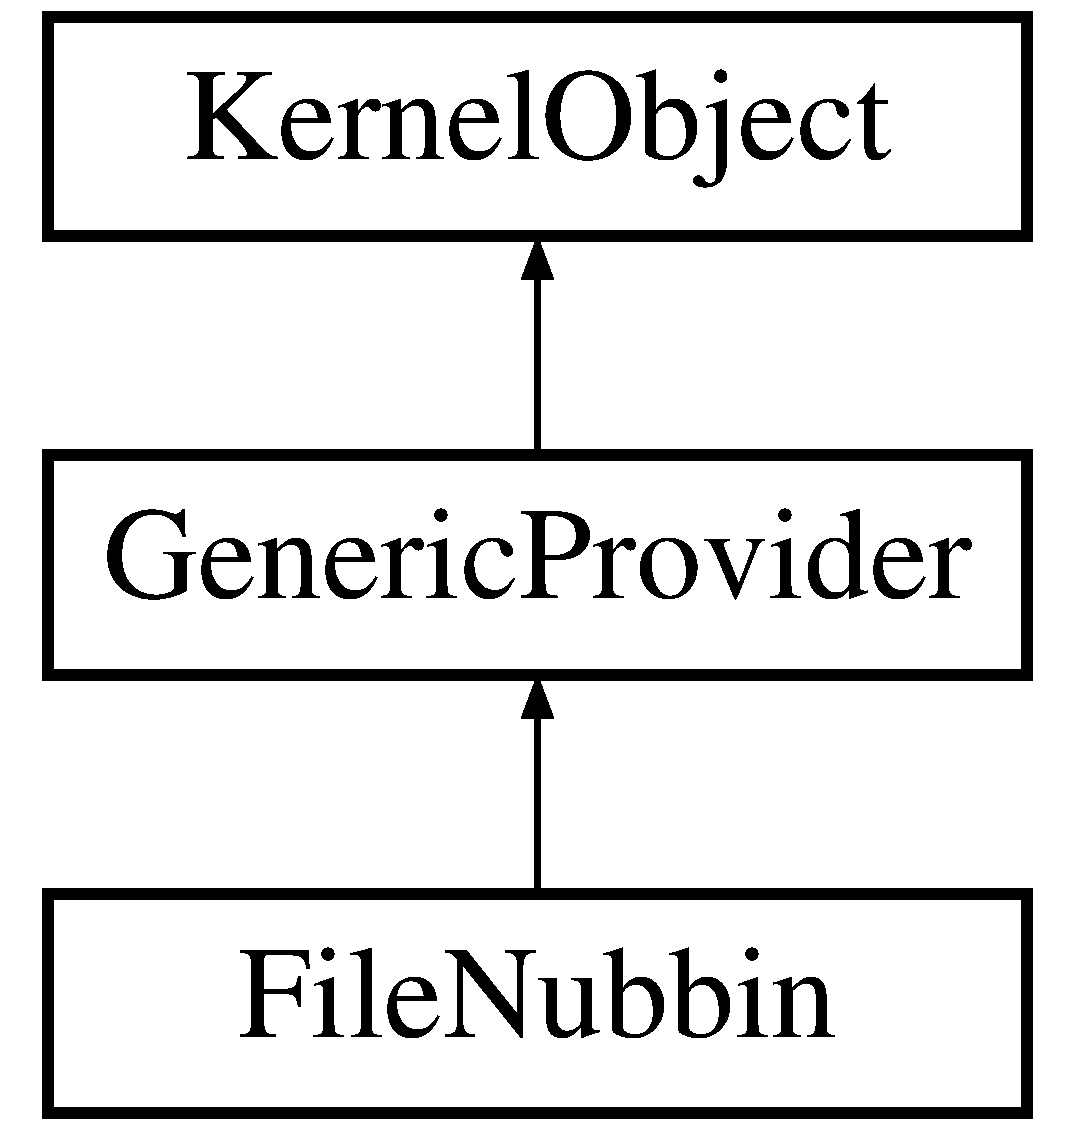
\includegraphics[height=3.000000cm]{class_file_nubbin}
\end{center}
\end{figure}
\subsection*{Public Member Functions}
\begin{DoxyCompactItemize}
\item 
\mbox{\Hypertarget{class_file_nubbin_a3610e343611cec037ed204aad82ce162}\label{class_file_nubbin_a3610e343611cec037ed204aad82ce162}} 
const char $\ast$ {\bfseries Get\+Class\+Name} (U\+Int32 level)
\end{DoxyCompactItemize}
\subsection*{Protected Member Functions}
\begin{DoxyCompactItemize}
\item 
\mbox{\Hypertarget{class_file_nubbin_a2d0dd708224d16f38bd65f5f9e58dcff}\label{class_file_nubbin_a2d0dd708224d16f38bd65f5f9e58dcff}} 
\hyperlink{class_generic_provider_1_1_input_connection}{Input\+Connection} $\ast$ {\bfseries Input\+Connection\+Start} (\hyperlink{class_kernel_string}{Kernel\+String} $\ast$name, \hyperlink{class_ipc_endpoint}{Ipc\+Endpoint} $\ast$connection)
\item 
\mbox{\Hypertarget{class_file_nubbin_a5892d0ab45aa3280c9a1d4ab9192a7c9}\label{class_file_nubbin_a5892d0ab45aa3280c9a1d4ab9192a7c9}} 
void {\bfseries Input\+Connection\+Received} (\hyperlink{class_generic_provider_1_1_input_connection}{Input\+Connection} $\ast$connection, \hyperlink{class_kernel_buffer_memory}{Kernel\+Buffer\+Memory} $\ast$message)
\item 
\mbox{\Hypertarget{class_file_nubbin_a5bd1d71596b948c2548d089f3f53bc4c}\label{class_file_nubbin_a5bd1d71596b948c2548d089f3f53bc4c}} 
void {\bfseries Input\+Connection\+End} (\hyperlink{class_generic_provider_1_1_input_connection}{Input\+Connection} $\ast$connection)
\item 
\mbox{\Hypertarget{class_file_nubbin_aaabd96992a6a9e608a1d0200c98ef05f}\label{class_file_nubbin_aaabd96992a6a9e608a1d0200c98ef05f}} 
\hyperlink{class_generic_provider_1_1_output_connection}{Output\+Connection} $\ast$ {\bfseries Output\+Connection\+Start} (\hyperlink{class_generic_provider_1_1_service}{Service} $\ast$source, \hyperlink{class_ipc_endpoint}{Ipc\+Endpoint} $\ast$connection)
\item 
\mbox{\Hypertarget{class_file_nubbin_a318d1408bfdfd7a927fd7b4a7be7a640}\label{class_file_nubbin_a318d1408bfdfd7a927fd7b4a7be7a640}} 
void {\bfseries Output\+Connection\+Message} (\hyperlink{class_generic_provider_1_1_output_connection}{Output\+Connection} $\ast$connection, \hyperlink{class_kernel_buffer_memory}{Kernel\+Buffer\+Memory} $\ast$message)
\item 
\mbox{\Hypertarget{class_file_nubbin_a3a4b7a025db8b6b423947bf921891072}\label{class_file_nubbin_a3a4b7a025db8b6b423947bf921891072}} 
void {\bfseries Output\+Connection\+End} (\hyperlink{class_generic_provider_1_1_output_connection}{Output\+Connection} $\ast$old\+Connection)
\end{DoxyCompactItemize}
\subsection*{Private Member Functions}
\begin{DoxyCompactItemize}
\item 
\mbox{\Hypertarget{class_file_nubbin_a9eeee47cc884ff7018c2aad7f5fef783}\label{class_file_nubbin_a9eeee47cc884ff7018c2aad7f5fef783}} 
\hyperlink{class_generic_provider_1_1_input_connection}{Input\+Connection} $\ast$ {\bfseries Input} (void)
\end{DoxyCompactItemize}
\subsection*{Private Attributes}
\begin{DoxyCompactItemize}
\item 
\mbox{\Hypertarget{class_file_nubbin_a8d5f1d19f134e6b2b15899080c8cbb78}\label{class_file_nubbin_a8d5f1d19f134e6b2b15899080c8cbb78}} 
\hyperlink{class_interface_helper}{Interface\+Helper} $\ast$ {\bfseries \+\_\+tasks}
\end{DoxyCompactItemize}
\subsection*{Additional Inherited Members}


The documentation for this class was generated from the following files\+:\begin{DoxyCompactItemize}
\item 
File\+Nubbin.\+h\item 
File\+Nubbin.\+cpp\end{DoxyCompactItemize}

\hypertarget{class_file_system___i_s_o9660}{}\section{File\+System\+\_\+\+I\+S\+O9660 Class Reference}
\label{class_file_system___i_s_o9660}\index{File\+System\+\_\+\+I\+S\+O9660@{File\+System\+\_\+\+I\+S\+O9660}}
Inheritance diagram for File\+System\+\_\+\+I\+S\+O9660\+:\begin{figure}[H]
\begin{center}
\leavevmode
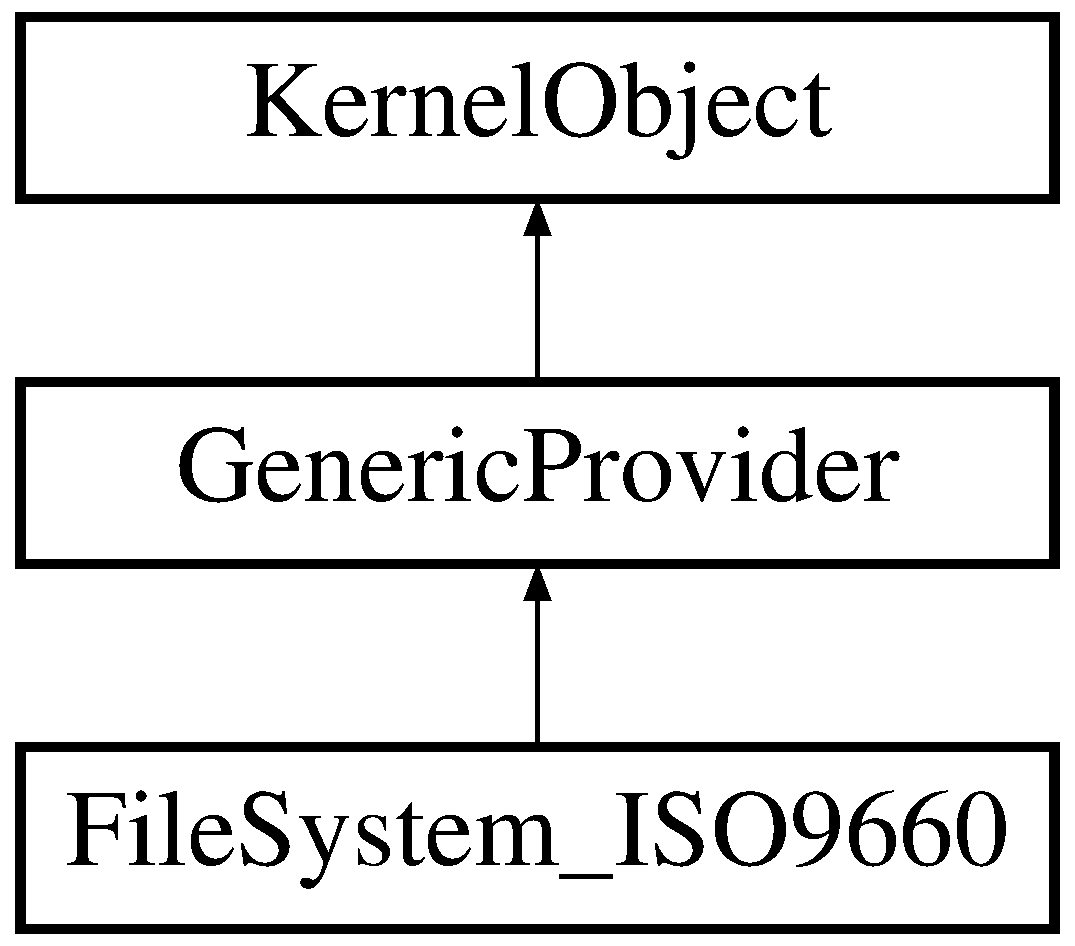
\includegraphics[height=3.000000cm]{class_file_system___i_s_o9660}
\end{center}
\end{figure}
\subsection*{Public Member Functions}
\begin{DoxyCompactItemize}
\item 
\mbox{\Hypertarget{class_file_system___i_s_o9660_ae48eb790c8be9145a59730ea53a73667}\label{class_file_system___i_s_o9660_ae48eb790c8be9145a59730ea53a73667}} 
const char $\ast$ {\bfseries Get\+Class\+Name} (U\+Int32 level)
\end{DoxyCompactItemize}
\subsection*{Protected Member Functions}
\begin{DoxyCompactItemize}
\item 
\mbox{\Hypertarget{class_file_system___i_s_o9660_aec75a25f049b5d49162737c020236f29}\label{class_file_system___i_s_o9660_aec75a25f049b5d49162737c020236f29}} 
\hyperlink{class_generic_provider_1_1_input_connection}{Input\+Connection} $\ast$ {\bfseries Input\+Connection\+Start} (\hyperlink{class_kernel_string}{Kernel\+String} $\ast$name, \hyperlink{class_ipc_endpoint}{Ipc\+Endpoint} $\ast$connection)
\item 
\mbox{\Hypertarget{class_file_system___i_s_o9660_aa8fc5bc6090dbaa4648837f133034543}\label{class_file_system___i_s_o9660_aa8fc5bc6090dbaa4648837f133034543}} 
void {\bfseries Input\+Connection\+Received} (\hyperlink{class_generic_provider_1_1_input_connection}{Input\+Connection} $\ast$connection, \hyperlink{class_kernel_buffer_memory}{Kernel\+Buffer\+Memory} $\ast$message)
\item 
\mbox{\Hypertarget{class_file_system___i_s_o9660_accad32bb3f7ec5d6bd3e4aa1ab75c72b}\label{class_file_system___i_s_o9660_accad32bb3f7ec5d6bd3e4aa1ab75c72b}} 
void {\bfseries Input\+Connection\+End} (\hyperlink{class_generic_provider_1_1_input_connection}{Input\+Connection} $\ast$connection)
\item 
\mbox{\Hypertarget{class_file_system___i_s_o9660_a65f08062655e64e11b6b04cd49f88648}\label{class_file_system___i_s_o9660_a65f08062655e64e11b6b04cd49f88648}} 
\hyperlink{class_generic_provider_1_1_output_connection}{Output\+Connection} $\ast$ {\bfseries Output\+Connection\+Start} (\hyperlink{class_generic_provider_1_1_service}{Service} $\ast$source, \hyperlink{class_ipc_endpoint}{Ipc\+Endpoint} $\ast$connection)
\item 
\mbox{\Hypertarget{class_file_system___i_s_o9660_aa3234131cd06c5b3aad307e206dc5eb4}\label{class_file_system___i_s_o9660_aa3234131cd06c5b3aad307e206dc5eb4}} 
void {\bfseries Output\+Connection\+Message} (\hyperlink{class_generic_provider_1_1_output_connection}{Output\+Connection} $\ast$connection, \hyperlink{class_kernel_buffer_memory}{Kernel\+Buffer\+Memory} $\ast$message)
\item 
\mbox{\Hypertarget{class_file_system___i_s_o9660_a5725b59566f7f9f97eae56a8caad85c4}\label{class_file_system___i_s_o9660_a5725b59566f7f9f97eae56a8caad85c4}} 
void {\bfseries Output\+Connection\+End} (\hyperlink{class_generic_provider_1_1_output_connection}{Output\+Connection} $\ast$old\+Connection)
\end{DoxyCompactItemize}
\subsection*{Private Member Functions}
\begin{DoxyCompactItemize}
\item 
\mbox{\Hypertarget{class_file_system___i_s_o9660_acfb7cd8374d0ec8065ac96545b759260}\label{class_file_system___i_s_o9660_acfb7cd8374d0ec8065ac96545b759260}} 
void {\bfseries Perform\+Task} (\hyperlink{class_ipc_endpoint}{Ipc\+Endpoint} $\ast$destination, \hyperlink{classbicycle_1_1function}{bicycle\+::function}$<$ int(Interface\+\_\+\+Request $\ast$)$>$ generate, \hyperlink{classbicycle_1_1function}{bicycle\+::function}$<$ int(Interface\+\_\+\+Response $\ast$)$>$ response)
\item 
\mbox{\Hypertarget{class_file_system___i_s_o9660_a10bd4494fa7f5ede324528c892462ac0}\label{class_file_system___i_s_o9660_a10bd4494fa7f5ede324528c892462ac0}} 
void {\bfseries Read\+G\+VD} (int offset)
\item 
\mbox{\Hypertarget{class_file_system___i_s_o9660_a8c423a8e7aa2d5abd4a598c6933472dc}\label{class_file_system___i_s_o9660_a8c423a8e7aa2d5abd4a598c6933472dc}} 
\hyperlink{class_generic_provider_1_1_input_connection}{Input\+Connection} $\ast$ {\bfseries Input} (void)
\item 
\mbox{\Hypertarget{class_file_system___i_s_o9660_a31d06e786de18d10b4b02c0d82c2a6d5}\label{class_file_system___i_s_o9660_a31d06e786de18d10b4b02c0d82c2a6d5}} 
void {\bfseries Ensure\+Entry\+Loaded} (\hyperlink{class_i_s_o9660_driver_1_1_generic_entry}{I\+S\+O9660\+Driver\+::\+Generic\+Entry} $\ast$entry, \hyperlink{classbicycle_1_1function}{bicycle\+::function}$<$ void(int)$>$ on\+Loaded)
\item 
\mbox{\Hypertarget{class_file_system___i_s_o9660_a67e4d00408d0fc5ec48aa5afc27c46c2}\label{class_file_system___i_s_o9660_a67e4d00408d0fc5ec48aa5afc27c46c2}} 
void {\bfseries Parse\+Path} (\hyperlink{class_i_s_o9660_driver_1_1_generic_entry}{I\+S\+O9660\+Driver\+::\+Generic\+Entry} $\ast$current, Flat\+Array $\ast$path, U\+Int32 path\+Index, \hyperlink{classbicycle_1_1function}{bicycle\+::function}$<$ void(\hyperlink{class_i_s_o9660_driver_1_1_generic_entry}{I\+S\+O9660\+Driver\+::\+Generic\+Entry} $\ast$)$>$ on\+Found, \hyperlink{classbicycle_1_1function}{bicycle\+::function}$<$ void(U\+Int32 failed\+Index, U\+Int32 reason)$>$ on\+Not\+Found)
\item 
\mbox{\Hypertarget{class_file_system___i_s_o9660_a823edd7eab33a4d9edb576b53d7ee1c0}\label{class_file_system___i_s_o9660_a823edd7eab33a4d9edb576b53d7ee1c0}} 
void {\bfseries Parse\+Path} (U\+Int64 start\+Node, Flat\+Array $\ast$path, U\+Int32 path\+Index, \hyperlink{classbicycle_1_1function}{bicycle\+::function}$<$ void(\hyperlink{class_i_s_o9660_driver_1_1_generic_entry}{I\+S\+O9660\+Driver\+::\+Generic\+Entry} $\ast$)$>$ on\+Found, \hyperlink{classbicycle_1_1function}{bicycle\+::function}$<$ void(U\+Int32 failed\+Index, U\+Int32 reason)$>$ on\+Not\+Found)
\end{DoxyCompactItemize}
\subsection*{Private Attributes}
\begin{DoxyCompactItemize}
\item 
\mbox{\Hypertarget{class_file_system___i_s_o9660_a19d8e4f30b4347fea84b70d7e02f7788}\label{class_file_system___i_s_o9660_a19d8e4f30b4347fea84b70d7e02f7788}} 
\hyperlink{class_i_s_o9660_driver_1_1_directory_entry}{I\+S\+O9660\+Driver\+::\+Directory\+Entry} $\ast$ {\bfseries \+\_\+root\+Directory}
\item 
\mbox{\Hypertarget{class_file_system___i_s_o9660_aa4c08b17b136cfaaae06b113335d6f14}\label{class_file_system___i_s_o9660_aa4c08b17b136cfaaae06b113335d6f14}} 
U\+Int64 {\bfseries \+\_\+node\+Counter}
\item 
\mbox{\Hypertarget{class_file_system___i_s_o9660_a53e621cc6d53322d1ea81adcb8c5fa1e}\label{class_file_system___i_s_o9660_a53e621cc6d53322d1ea81adcb8c5fa1e}} 
\hyperlink{class_interface_helper}{Interface\+Helper} $\ast$ {\bfseries \+\_\+tasks}
\end{DoxyCompactItemize}
\subsection*{Additional Inherited Members}


The documentation for this class was generated from the following files\+:\begin{DoxyCompactItemize}
\item 
fs\+\_\+iso9660.\+h\item 
fs\+\_\+iso9660.\+cpp\end{DoxyCompactItemize}

\hypertarget{class_c_p_u_1_1_f_p_u_context}{}\section{C\+PU\+:\+:F\+P\+U\+Context Class Reference}
\label{class_c_p_u_1_1_f_p_u_context}\index{C\+P\+U\+::\+F\+P\+U\+Context@{C\+P\+U\+::\+F\+P\+U\+Context}}
\subsection*{Public Member Functions}
\begin{DoxyCompactItemize}
\item 
\mbox{\Hypertarget{class_c_p_u_1_1_f_p_u_context_a2049972f314c95d4b2b6eaeb8bec01cd}\label{class_c_p_u_1_1_f_p_u_context_a2049972f314c95d4b2b6eaeb8bec01cd}} 
void {\bfseries Store} (void)
\item 
\mbox{\Hypertarget{class_c_p_u_1_1_f_p_u_context_ac3585931eb5408f7ed40966f582fc85e}\label{class_c_p_u_1_1_f_p_u_context_ac3585931eb5408f7ed40966f582fc85e}} 
void {\bfseries Restore} (void)
\end{DoxyCompactItemize}
\subsection*{Public Attributes}
\begin{DoxyCompactItemize}
\item 
\mbox{\Hypertarget{class_c_p_u_1_1_f_p_u_context_acf8229836e3e097a0b9cb27931492424}\label{class_c_p_u_1_1_f_p_u_context_acf8229836e3e097a0b9cb27931492424}} 
char {\bfseries data} \mbox{[}108\mbox{]}
\end{DoxyCompactItemize}


The documentation for this class was generated from the following file\+:\begin{DoxyCompactItemize}
\item 
C\+P\+U.\+h\end{DoxyCompactItemize}

\hypertarget{struct_generic_video_1_1_f_r_a_m_e_b_u_f_f_e_r}{}\section{Generic\+Video\+:\+:F\+R\+A\+M\+E\+B\+U\+F\+F\+ER Struct Reference}
\label{struct_generic_video_1_1_f_r_a_m_e_b_u_f_f_e_r}\index{Generic\+Video\+::\+F\+R\+A\+M\+E\+B\+U\+F\+F\+ER@{Generic\+Video\+::\+F\+R\+A\+M\+E\+B\+U\+F\+F\+ER}}
\subsection*{Public Types}
\begin{DoxyCompactItemize}
\item 
\mbox{\Hypertarget{struct_generic_video_1_1_f_r_a_m_e_b_u_f_f_e_r_a38bd8d779b5d02419d1849f009d6f158}\label{struct_generic_video_1_1_f_r_a_m_e_b_u_f_f_e_r_a38bd8d779b5d02419d1849f009d6f158}} 
enum {\bfseries Pixel\+Format} \{ {\bfseries Pixel24\+R\+GB}, 
{\bfseries Pixel24\+B\+GR}, 
{\bfseries Pixel32\+R\+G\+Bx}, 
{\bfseries Pixel32\+B\+G\+Rx}
 \}
\end{DoxyCompactItemize}
\subsection*{Public Attributes}
\begin{DoxyCompactItemize}
\item 
\mbox{\Hypertarget{struct_generic_video_1_1_f_r_a_m_e_b_u_f_f_e_r_a954cd6b182ab1df0758616917ddcf064}\label{struct_generic_video_1_1_f_r_a_m_e_b_u_f_f_e_r_a954cd6b182ab1df0758616917ddcf064}} 
int {\bfseries width}
\item 
\mbox{\Hypertarget{struct_generic_video_1_1_f_r_a_m_e_b_u_f_f_e_r_a527a99a438df1a46909f18ffdde7ffcb}\label{struct_generic_video_1_1_f_r_a_m_e_b_u_f_f_e_r_a527a99a438df1a46909f18ffdde7ffcb}} 
int {\bfseries height}
\item 
\mbox{\Hypertarget{struct_generic_video_1_1_f_r_a_m_e_b_u_f_f_e_r_a3357709abff25112e53ca4bdcb43cf00}\label{struct_generic_video_1_1_f_r_a_m_e_b_u_f_f_e_r_a3357709abff25112e53ca4bdcb43cf00}} 
T\+Y\+PE {\bfseries mode}
\item 
\mbox{\Hypertarget{struct_generic_video_1_1_f_r_a_m_e_b_u_f_f_e_r_a01fc057b3adee75af9528dd1953ee4ad}\label{struct_generic_video_1_1_f_r_a_m_e_b_u_f_f_e_r_a01fc057b3adee75af9528dd1953ee4ad}} 
Physical\+Pointer {\bfseries address}
\item 
\mbox{\Hypertarget{struct_generic_video_1_1_f_r_a_m_e_b_u_f_f_e_r_af15f6a049da78198065915d9ba9e99a4}\label{struct_generic_video_1_1_f_r_a_m_e_b_u_f_f_e_r_af15f6a049da78198065915d9ba9e99a4}} 
int {\bfseries line\+Span}
\item 
\mbox{\Hypertarget{struct_generic_video_1_1_f_r_a_m_e_b_u_f_f_e_r_a78459a43694cb0d452c5878768c47318}\label{struct_generic_video_1_1_f_r_a_m_e_b_u_f_f_e_r_a78459a43694cb0d452c5878768c47318}} 
int {\bfseries bytes\+Per\+Pixel}
\item 
\mbox{\Hypertarget{struct_generic_video_1_1_f_r_a_m_e_b_u_f_f_e_r_a06d74f3ca675e5bad576701a220deaee}\label{struct_generic_video_1_1_f_r_a_m_e_b_u_f_f_e_r_a06d74f3ca675e5bad576701a220deaee}} 
Pixel\+Format {\bfseries format}
\end{DoxyCompactItemize}


The documentation for this struct was generated from the following file\+:\begin{DoxyCompactItemize}
\item 
Generic\+Video.\+h\end{DoxyCompactItemize}

\hypertarget{class_internal_1_1_free_space}{}\section{Internal\+:\+:Free\+Space Class Reference}
\label{class_internal_1_1_free_space}\index{Internal\+::\+Free\+Space@{Internal\+::\+Free\+Space}}
Inheritance diagram for Internal\+:\+:Free\+Space\+:\begin{figure}[H]
\begin{center}
\leavevmode
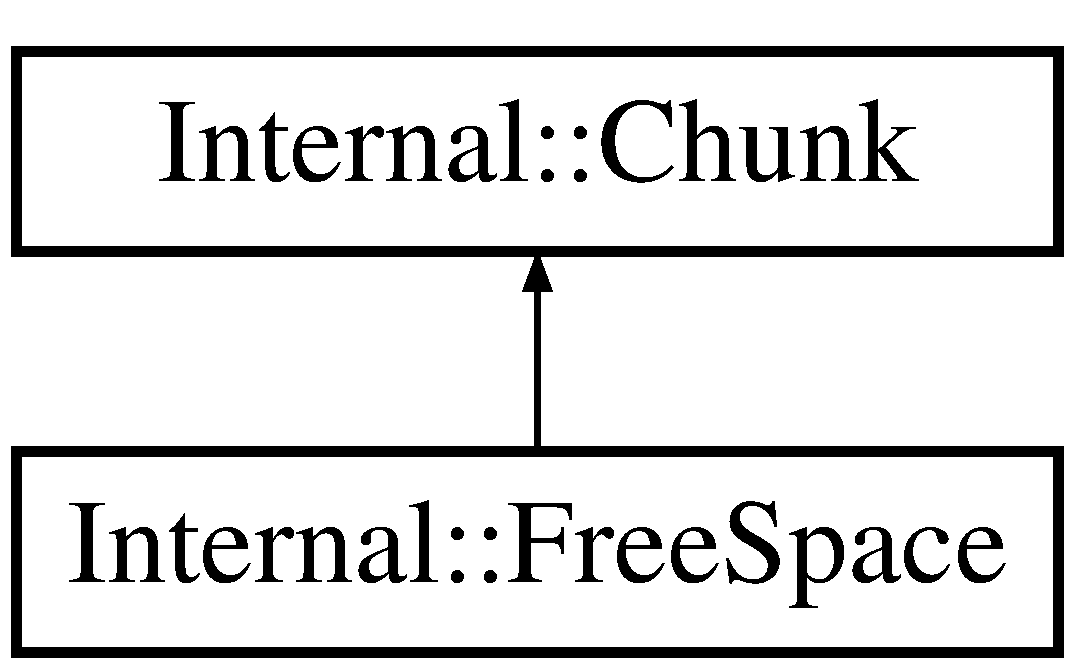
\includegraphics[height=2.000000cm]{class_internal_1_1_free_space}
\end{center}
\end{figure}
\subsection*{Public Member Functions}
\begin{DoxyCompactItemize}
\item 
\mbox{\Hypertarget{class_internal_1_1_free_space_aa49a37f66e5839379a2be70f4a014515}\label{class_internal_1_1_free_space_aa49a37f66e5839379a2be70f4a014515}} 
{\bfseries Free\+Space} (\hyperlink{class_basic_heap}{Basic\+Heap} $\ast$owner, Basic\+Heap\+::h\+\_\+size size)
\item 
\mbox{\Hypertarget{class_internal_1_1_free_space_ab3d263aa397c45d8be07e66d715cdfee}\label{class_internal_1_1_free_space_ab3d263aa397c45d8be07e66d715cdfee}} 
\hyperlink{class_internal_1_1_free_space}{Free\+Space} $\ast$ {\bfseries Split} (Basic\+Heap\+::h\+\_\+size size)
\item 
\mbox{\Hypertarget{class_internal_1_1_free_space_ac001c0431b6942012e7d03f30937eb4c}\label{class_internal_1_1_free_space_ac001c0431b6942012e7d03f30937eb4c}} 
int {\bfseries Merge} (void)
\end{DoxyCompactItemize}
\subsection*{Public Attributes}
\begin{DoxyCompactItemize}
\item 
\mbox{\Hypertarget{class_internal_1_1_free_space_ad8ef6322f41635762ac8bb03e109ad14}\label{class_internal_1_1_free_space_ad8ef6322f41635762ac8bb03e109ad14}} 
\hyperlink{class_internal_1_1_free_space}{Free\+Space} $\ast$ {\bfseries last}
\item 
\mbox{\Hypertarget{class_internal_1_1_free_space_a7f23ff600c1e06b38c41cd1babb6e4b4}\label{class_internal_1_1_free_space_a7f23ff600c1e06b38c41cd1babb6e4b4}} 
\hyperlink{class_internal_1_1_free_space}{Free\+Space} $\ast$ {\bfseries next}
\end{DoxyCompactItemize}
\subsection*{Private Attributes}
\begin{DoxyCompactItemize}
\item 
\mbox{\Hypertarget{class_internal_1_1_free_space_aa88e61b5d518682778c5c72764cad7b4}\label{class_internal_1_1_free_space_aa88e61b5d518682778c5c72764cad7b4}} 
\hyperlink{class_basic_heap}{Basic\+Heap} $\ast$ {\bfseries \+\_\+heap}
\end{DoxyCompactItemize}
\subsection*{Additional Inherited Members}


The documentation for this class was generated from the following file\+:\begin{DoxyCompactItemize}
\item 
Basic\+Heap.\+cpp\end{DoxyCompactItemize}

\hypertarget{structbicycle_1_1func__filter}{}\section{bicycle\+:\+:func\+\_\+filter$<$ Func $>$ Struct Template Reference}
\label{structbicycle_1_1func__filter}\index{bicycle\+::func\+\_\+filter$<$ Func $>$@{bicycle\+::func\+\_\+filter$<$ Func $>$}}
\subsection*{Public Types}
\begin{DoxyCompactItemize}
\item 
\mbox{\Hypertarget{structbicycle_1_1func__filter_a6388729a15d62e3c7d9ca550d9d9da3b}\label{structbicycle_1_1func__filter_a6388729a15d62e3c7d9ca550d9d9da3b}} 
typedef Func {\bfseries type}
\end{DoxyCompactItemize}


The documentation for this struct was generated from the following file\+:\begin{DoxyCompactItemize}
\item 
Kernel\+Function.\+h\end{DoxyCompactItemize}

\hypertarget{structbicycle_1_1func__filter_3_01_result_07_args_8_8_8_08_4}{}\section{bicycle\+:\+:func\+\_\+filter$<$ Result(Args...)$>$ Struct Template Reference}
\label{structbicycle_1_1func__filter_3_01_result_07_args_8_8_8_08_4}\index{bicycle\+::func\+\_\+filter$<$ Result(\+Args...)$>$@{bicycle\+::func\+\_\+filter$<$ Result(\+Args...)$>$}}
\subsection*{Public Types}
\begin{DoxyCompactItemize}
\item 
\mbox{\Hypertarget{structbicycle_1_1func__filter_3_01_result_07_args_8_8_8_08_4_a4cc2a468603b62d2c6639d9cad87d825}\label{structbicycle_1_1func__filter_3_01_result_07_args_8_8_8_08_4_a4cc2a468603b62d2c6639d9cad87d825}} 
typedef Result($\ast$ {\bfseries type}) (Args...)
\end{DoxyCompactItemize}


The documentation for this struct was generated from the following file\+:\begin{DoxyCompactItemize}
\item 
Kernel\+Function.\+h\end{DoxyCompactItemize}

\hypertarget{classbicycle_1_1function}{}\section{bicycle\+:\+:function$<$ signature $>$ Class Template Reference}
\label{classbicycle_1_1function}\index{bicycle\+::function$<$ signature $>$@{bicycle\+::function$<$ signature $>$}}


The documentation for this class was generated from the following file\+:\begin{DoxyCompactItemize}
\item 
Kernel\+Function.\+h\end{DoxyCompactItemize}

\hypertarget{classbicycle_1_1function_3_01_result_07_args_8_8_8_08_4}{}\section{bicycle\+:\+:function$<$ Result(Args...)$>$ Class Template Reference}
\label{classbicycle_1_1function_3_01_result_07_args_8_8_8_08_4}\index{bicycle\+::function$<$ Result(\+Args...)$>$@{bicycle\+::function$<$ Result(\+Args...)$>$}}
\subsection*{Public Member Functions}
\begin{DoxyCompactItemize}
\item 
\mbox{\Hypertarget{classbicycle_1_1function_3_01_result_07_args_8_8_8_08_4_a406cca8012390e9d9c7beb625fc2f8be}\label{classbicycle_1_1function_3_01_result_07_args_8_8_8_08_4_a406cca8012390e9d9c7beb625fc2f8be}} 
{\footnotesize template$<$typename Func $>$ }\\{\bfseries function} (const Func \&x)
\item 
\mbox{\Hypertarget{classbicycle_1_1function_3_01_result_07_args_8_8_8_08_4_a2de0e18109cc2ffd292e7469019e60bf}\label{classbicycle_1_1function_3_01_result_07_args_8_8_8_08_4_a2de0e18109cc2ffd292e7469019e60bf}} 
{\bfseries function} (const \hyperlink{classbicycle_1_1function}{function} \&rhs)
\item 
\mbox{\Hypertarget{classbicycle_1_1function_3_01_result_07_args_8_8_8_08_4_a05d7b7d0ff1d9d0e543e23c17c08ee1d}\label{classbicycle_1_1function_3_01_result_07_args_8_8_8_08_4_a05d7b7d0ff1d9d0e543e23c17c08ee1d}} 
\hyperlink{classbicycle_1_1function}{function} \& {\bfseries operator=} (const \hyperlink{classbicycle_1_1function}{function} \&rhs)
\item 
\mbox{\Hypertarget{classbicycle_1_1function_3_01_result_07_args_8_8_8_08_4_a35979bc6f350a35287291d811016f442}\label{classbicycle_1_1function_3_01_result_07_args_8_8_8_08_4_a35979bc6f350a35287291d811016f442}} 
{\footnotesize template$<$typename Func $>$ }\\\hyperlink{classbicycle_1_1function}{function} \& {\bfseries operator=} (const Func \&x)
\item 
\mbox{\Hypertarget{classbicycle_1_1function_3_01_result_07_args_8_8_8_08_4_a35bdb499145776c993b6b6b7ae8432cf}\label{classbicycle_1_1function_3_01_result_07_args_8_8_8_08_4_a35bdb499145776c993b6b6b7ae8432cf}} 
Result {\bfseries operator()} (Args... args) const
\end{DoxyCompactItemize}
\subsection*{Private Attributes}
\begin{DoxyCompactItemize}
\item 
\mbox{\Hypertarget{classbicycle_1_1function_3_01_result_07_args_8_8_8_08_4_a67d4aa030a44c2bcfe5f797723e8d1c9}\label{classbicycle_1_1function_3_01_result_07_args_8_8_8_08_4_a67d4aa030a44c2bcfe5f797723e8d1c9}} 
\hyperlink{structbicycle_1_1abstract__function}{abstract\+\_\+function}$<$ Result, Args... $>$ $\ast$ {\bfseries f}
\end{DoxyCompactItemize}


The documentation for this class was generated from the following file\+:\begin{DoxyCompactItemize}
\item 
Kernel\+Function.\+h\end{DoxyCompactItemize}

\hypertarget{classbicycle_1_1function_3_01void_07_args_8_8_8_08_4}{}\section{bicycle\+:\+:function$<$ void(Args...)$>$ Class Template Reference}
\label{classbicycle_1_1function_3_01void_07_args_8_8_8_08_4}\index{bicycle\+::function$<$ void(\+Args...)$>$@{bicycle\+::function$<$ void(\+Args...)$>$}}
\subsection*{Public Member Functions}
\begin{DoxyCompactItemize}
\item 
\mbox{\Hypertarget{classbicycle_1_1function_3_01void_07_args_8_8_8_08_4_a7652f084a4b89af8e913ec658a4e0ca5}\label{classbicycle_1_1function_3_01void_07_args_8_8_8_08_4_a7652f084a4b89af8e913ec658a4e0ca5}} 
{\footnotesize template$<$typename Func $>$ }\\{\bfseries function} (const Func \&x)
\item 
\mbox{\Hypertarget{classbicycle_1_1function_3_01void_07_args_8_8_8_08_4_af2421e7cfdca2755169a449445977af2}\label{classbicycle_1_1function_3_01void_07_args_8_8_8_08_4_af2421e7cfdca2755169a449445977af2}} 
{\bfseries function} (const \hyperlink{classbicycle_1_1function}{function} \&rhs)
\item 
\mbox{\Hypertarget{classbicycle_1_1function_3_01void_07_args_8_8_8_08_4_a057e6eed484cc06322126726b6b56a78}\label{classbicycle_1_1function_3_01void_07_args_8_8_8_08_4_a057e6eed484cc06322126726b6b56a78}} 
\hyperlink{classbicycle_1_1function}{function} \& {\bfseries operator=} (const \hyperlink{classbicycle_1_1function}{function} \&rhs)
\item 
\mbox{\Hypertarget{classbicycle_1_1function_3_01void_07_args_8_8_8_08_4_a062e23deb6c976c3a1fabc293428237c}\label{classbicycle_1_1function_3_01void_07_args_8_8_8_08_4_a062e23deb6c976c3a1fabc293428237c}} 
{\footnotesize template$<$typename Func $>$ }\\\hyperlink{classbicycle_1_1function}{function} \& {\bfseries operator=} (const Func \&x)
\item 
\mbox{\Hypertarget{classbicycle_1_1function_3_01void_07_args_8_8_8_08_4_aa77bb97b31ca2abe49357405bbbce6bd}\label{classbicycle_1_1function_3_01void_07_args_8_8_8_08_4_aa77bb97b31ca2abe49357405bbbce6bd}} 
void {\bfseries operator()} (Args... args) const
\end{DoxyCompactItemize}
\subsection*{Private Attributes}
\begin{DoxyCompactItemize}
\item 
\mbox{\Hypertarget{classbicycle_1_1function_3_01void_07_args_8_8_8_08_4_a0f880231a4e0d21d1cb8290b887dd4bb}\label{classbicycle_1_1function_3_01void_07_args_8_8_8_08_4_a0f880231a4e0d21d1cb8290b887dd4bb}} 
\hyperlink{structbicycle_1_1abstract__function}{abstract\+\_\+function}$<$ void, Args... $>$ $\ast$ {\bfseries f}
\end{DoxyCompactItemize}


The documentation for this class was generated from the following file\+:\begin{DoxyCompactItemize}
\item 
Kernel\+Function.\+h\end{DoxyCompactItemize}

\hypertarget{class_i_s_o9660_driver_1_1_generic_entry}{}\section{I\+S\+O9660\+Driver\+:\+:Generic\+Entry Class Reference}
\label{class_i_s_o9660_driver_1_1_generic_entry}\index{I\+S\+O9660\+Driver\+::\+Generic\+Entry@{I\+S\+O9660\+Driver\+::\+Generic\+Entry}}
Inheritance diagram for I\+S\+O9660\+Driver\+:\+:Generic\+Entry\+:\begin{figure}[H]
\begin{center}
\leavevmode
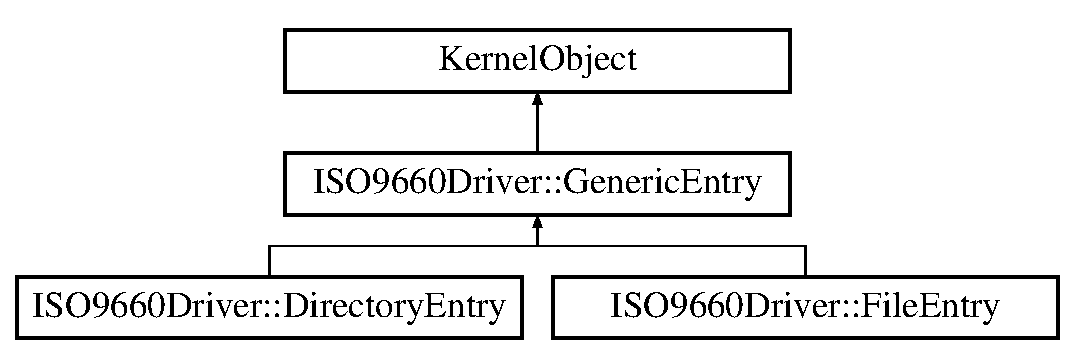
\includegraphics[height=3.000000cm]{class_i_s_o9660_driver_1_1_generic_entry}
\end{center}
\end{figure}
\subsection*{Classes}
\begin{DoxyCompactItemize}
\item 
class \hyperlink{class_i_s_o9660_driver_1_1_generic_entry_1_1_interim_date}{Interim\+Date}
\end{DoxyCompactItemize}
\subsection*{Public Member Functions}
\begin{DoxyCompactItemize}
\item 
\mbox{\Hypertarget{class_i_s_o9660_driver_1_1_generic_entry_a0c52498ba3b8d3ea4fc94917a189f644}\label{class_i_s_o9660_driver_1_1_generic_entry_a0c52498ba3b8d3ea4fc94917a189f644}} 
const char $\ast$ {\bfseries Get\+Class\+Name} (U\+Int32 level)
\item 
\mbox{\Hypertarget{class_i_s_o9660_driver_1_1_generic_entry_adb6933e6011e07c57785824d45b63962}\label{class_i_s_o9660_driver_1_1_generic_entry_adb6933e6011e07c57785824d45b63962}} 
{\bfseries Generic\+Entry} (const Directory\+Record $\ast$record)
\item 
\mbox{\Hypertarget{class_i_s_o9660_driver_1_1_generic_entry_ab48b924fed6721e2063e748bb92b2cf2}\label{class_i_s_o9660_driver_1_1_generic_entry_ab48b924fed6721e2063e748bb92b2cf2}} 
bool {\bfseries Is\+Directory} (void)
\item 
\mbox{\Hypertarget{class_i_s_o9660_driver_1_1_generic_entry_abdf8c027359d53e1a6fdf1d8927789e0}\label{class_i_s_o9660_driver_1_1_generic_entry_abdf8c027359d53e1a6fdf1d8927789e0}} 
void {\bfseries Encode} (Flat\+Dictionary $\ast$output)
\end{DoxyCompactItemize}
\subsection*{Public Attributes}
\begin{DoxyCompactItemize}
\item 
\mbox{\Hypertarget{class_i_s_o9660_driver_1_1_generic_entry_a3e4b5da3520ee802a7aec03d8c7589eb}\label{class_i_s_o9660_driver_1_1_generic_entry_a3e4b5da3520ee802a7aec03d8c7589eb}} 
U\+Int32 {\bfseries node}
\item 
\mbox{\Hypertarget{class_i_s_o9660_driver_1_1_generic_entry_a281aeac84ff6fed9afba7fa99ab076ca}\label{class_i_s_o9660_driver_1_1_generic_entry_a281aeac84ff6fed9afba7fa99ab076ca}} 
U\+Int32 {\bfseries start}
\item 
\mbox{\Hypertarget{class_i_s_o9660_driver_1_1_generic_entry_ad5af615529f2823846f1205b9a3fea8f}\label{class_i_s_o9660_driver_1_1_generic_entry_ad5af615529f2823846f1205b9a3fea8f}} 
U\+Int32 {\bfseries length}
\item 
\mbox{\Hypertarget{class_i_s_o9660_driver_1_1_generic_entry_a8e4ca44b4109033c6b526b01daffc87c}\label{class_i_s_o9660_driver_1_1_generic_entry_a8e4ca44b4109033c6b526b01daffc87c}} 
\hyperlink{class_kernel_string}{Kernel\+String} $\ast$ {\bfseries name}
\end{DoxyCompactItemize}
\subsection*{Static Private Member Functions}
\begin{DoxyCompactItemize}
\item 
\mbox{\Hypertarget{class_i_s_o9660_driver_1_1_generic_entry_a60d478f922eed16f71ee2bd8b736438f}\label{class_i_s_o9660_driver_1_1_generic_entry_a60d478f922eed16f71ee2bd8b736438f}} 
static void {\bfseries Save\+String} (Flat\+Array $\ast$output, const char $\ast$key)
\item 
\mbox{\Hypertarget{class_i_s_o9660_driver_1_1_generic_entry_a4f6823d68ad344923d24a35e781fbd29}\label{class_i_s_o9660_driver_1_1_generic_entry_a4f6823d68ad344923d24a35e781fbd29}} 
static void {\bfseries Save\+Integer} (Flat\+Array $\ast$output, U\+Int64 value)
\end{DoxyCompactItemize}
\subsection*{Private Attributes}
\begin{DoxyCompactItemize}
\item 
\mbox{\Hypertarget{class_i_s_o9660_driver_1_1_generic_entry_a3be07e0ee32ce5577cbb44b5bd7d9cc6}\label{class_i_s_o9660_driver_1_1_generic_entry_a3be07e0ee32ce5577cbb44b5bd7d9cc6}} 
bool {\bfseries \+\_\+is\+Directory}
\item 
\mbox{\Hypertarget{class_i_s_o9660_driver_1_1_generic_entry_a8e5b26bece08a4775b6d329c0458b4ed}\label{class_i_s_o9660_driver_1_1_generic_entry_a8e5b26bece08a4775b6d329c0458b4ed}} 
\hyperlink{class_i_s_o9660_driver_1_1_generic_entry_1_1_interim_date}{Interim\+Date} {\bfseries \+\_\+creation\+Date}
\end{DoxyCompactItemize}
\subsection*{Additional Inherited Members}


The documentation for this class was generated from the following file\+:\begin{DoxyCompactItemize}
\item 
fs\+\_\+iso9660.\+cpp\end{DoxyCompactItemize}

\hypertarget{class_a_t_a_driver_drive_1_1_generic_handler}{}\section{A\+T\+A\+Driver\+Drive\+:\+:Generic\+Handler Class Reference}
\label{class_a_t_a_driver_drive_1_1_generic_handler}\index{A\+T\+A\+Driver\+Drive\+::\+Generic\+Handler@{A\+T\+A\+Driver\+Drive\+::\+Generic\+Handler}}
Inheritance diagram for A\+T\+A\+Driver\+Drive\+:\+:Generic\+Handler\+:\begin{figure}[H]
\begin{center}
\leavevmode
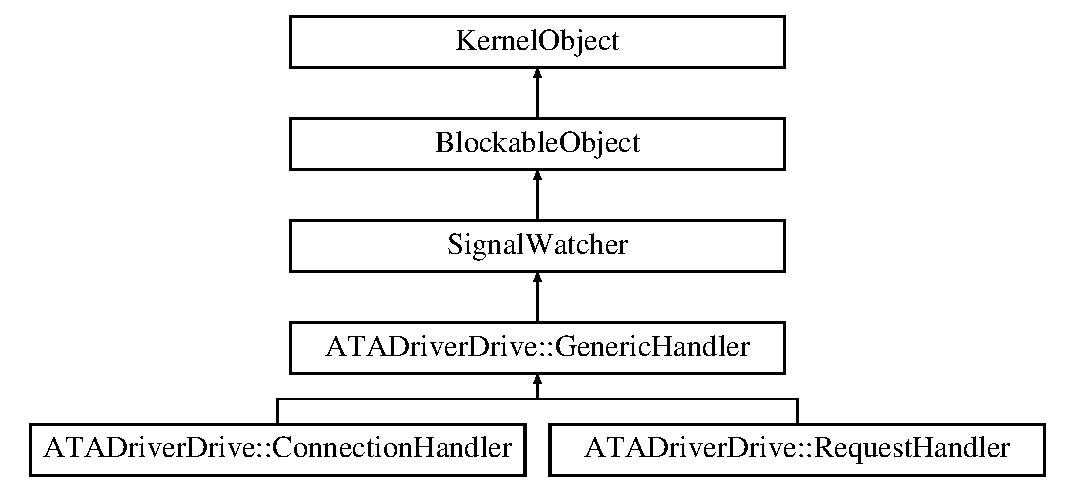
\includegraphics[height=5.000000cm]{class_a_t_a_driver_drive_1_1_generic_handler}
\end{center}
\end{figure}
\subsection*{Public Member Functions}
\begin{DoxyCompactItemize}
\item 
\mbox{\Hypertarget{class_a_t_a_driver_drive_1_1_generic_handler_a7998229768c9be84cf6162f52815e5b4}\label{class_a_t_a_driver_drive_1_1_generic_handler_a7998229768c9be84cf6162f52815e5b4}} 
const char $\ast$ {\bfseries Get\+Class\+Name} (U\+Int32 level)
\item 
\mbox{\Hypertarget{class_a_t_a_driver_drive_1_1_generic_handler_affba10bc475e4b471ce76f4e76206e0f}\label{class_a_t_a_driver_drive_1_1_generic_handler_affba10bc475e4b471ce76f4e76206e0f}} 
{\bfseries Generic\+Handler} (\hyperlink{class_a_t_a_driver_drive}{A\+T\+A\+Driver\+Drive} $\ast$owner)
\end{DoxyCompactItemize}
\subsection*{Protected Attributes}
\begin{DoxyCompactItemize}
\item 
\mbox{\Hypertarget{class_a_t_a_driver_drive_1_1_generic_handler_a0e1a78771ea3f6c40925d9dfe0f6d34c}\label{class_a_t_a_driver_drive_1_1_generic_handler_a0e1a78771ea3f6c40925d9dfe0f6d34c}} 
\hyperlink{class_a_t_a_driver_drive}{A\+T\+A\+Driver\+Drive} $\ast$ {\bfseries \+\_\+owner}
\end{DoxyCompactItemize}
\subsection*{Additional Inherited Members}


The documentation for this class was generated from the following file\+:\begin{DoxyCompactItemize}
\item 
Driver\+\_\+\+A\+T\+A.\+cpp\end{DoxyCompactItemize}

\hypertarget{class_generic_keyboard}{}\section{Generic\+Keyboard Class Reference}
\label{class_generic_keyboard}\index{Generic\+Keyboard@{Generic\+Keyboard}}
Inheritance diagram for Generic\+Keyboard\+:\begin{figure}[H]
\begin{center}
\leavevmode
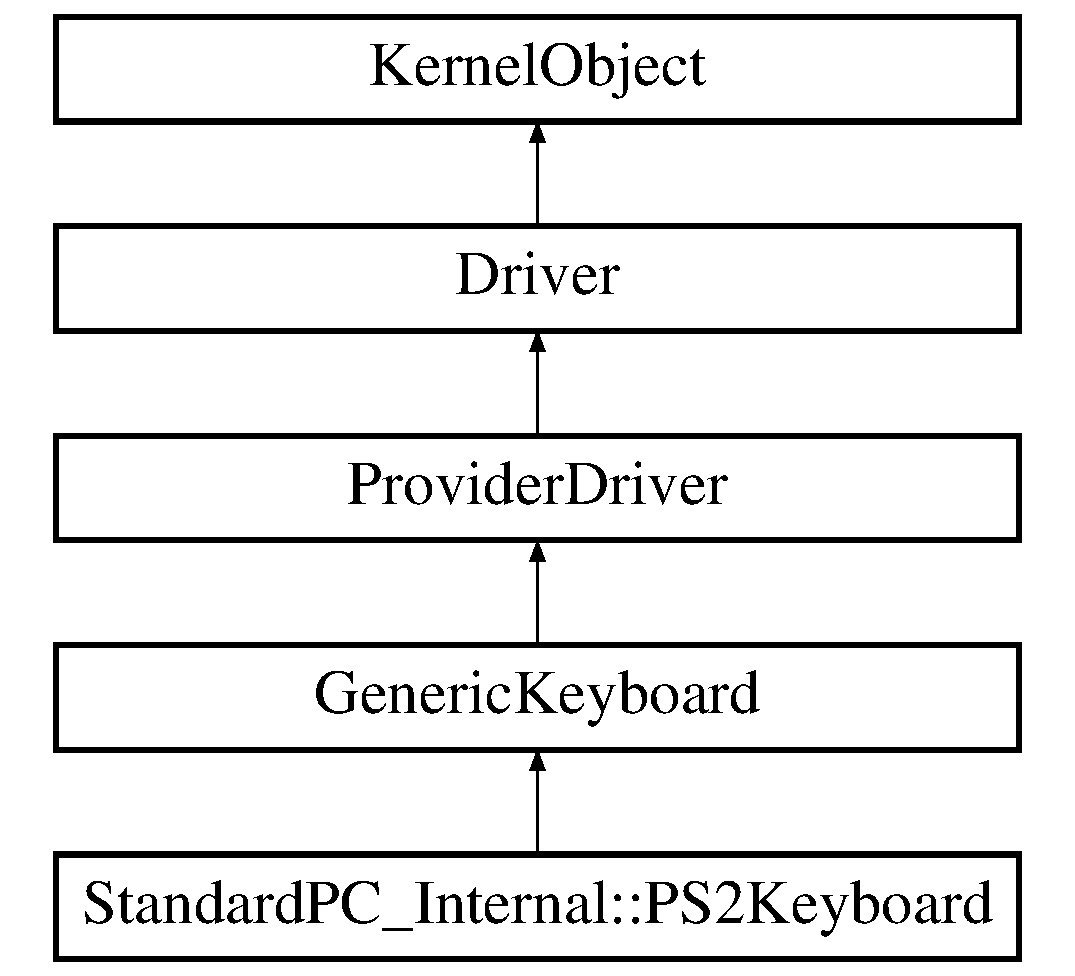
\includegraphics[height=5.000000cm]{class_generic_keyboard}
\end{center}
\end{figure}
\subsection*{Public Member Functions}
\begin{DoxyCompactItemize}
\item 
\mbox{\Hypertarget{class_generic_keyboard_ada61b732d8ef64c5a506896f4fbeee87}\label{class_generic_keyboard_ada61b732d8ef64c5a506896f4fbeee87}} 
const char $\ast$ {\bfseries Get\+Class\+Name} (U\+Int32 level)
\item 
\mbox{\Hypertarget{class_generic_keyboard_a3df84388c4aca9eb633d259f6cf670ed}\label{class_generic_keyboard_a3df84388c4aca9eb633d259f6cf670ed}} 
{\bfseries Generic\+Keyboard} (const char $\ast$name)
\item 
\mbox{\Hypertarget{class_generic_keyboard_a437887f81eb3507c4e9775127040eb26}\label{class_generic_keyboard_a437887f81eb3507c4e9775127040eb26}} 
bool {\bfseries Start} (\hyperlink{class_driver}{Driver} $\ast$parent)
\item 
\mbox{\Hypertarget{class_generic_keyboard_acc9f38c7e0a6a3d1adf545fdddd31388}\label{class_generic_keyboard_acc9f38c7e0a6a3d1adf545fdddd31388}} 
void {\bfseries Stop} (void)
\end{DoxyCompactItemize}
\subsection*{Protected Member Functions}
\begin{DoxyCompactItemize}
\item 
\mbox{\Hypertarget{class_generic_keyboard_a7e7e2702466ab806a76e1db77adc832a}\label{class_generic_keyboard_a7e7e2702466ab806a76e1db77adc832a}} 
bool {\bfseries Handle\+Key} (U\+Int8 event)
\item 
\mbox{\Hypertarget{class_generic_keyboard_ae3a3b36c55bf4761fe69fed8f4579ac2}\label{class_generic_keyboard_ae3a3b36c55bf4761fe69fed8f4579ac2}} 
void {\bfseries Send\+Event} (int key, bool down)
\item 
\mbox{\Hypertarget{class_generic_keyboard_a1582672c49773e3095c25d5b73991d57}\label{class_generic_keyboard_a1582672c49773e3095c25d5b73991d57}} 
\hyperlink{class_provider_driver_1_1_connection}{Connection} $\ast$ {\bfseries Connection\+Start} (Service $\ast$service, \hyperlink{class_ipc_endpoint}{Ipc\+Endpoint} $\ast$endpoint)
\item 
\mbox{\Hypertarget{class_generic_keyboard_a334c6ddbc5046b15d7096132e6473107}\label{class_generic_keyboard_a334c6ddbc5046b15d7096132e6473107}} 
void {\bfseries Connection\+Receive} (\hyperlink{class_provider_driver_1_1_connection}{Connection} $\ast$connection, \hyperlink{class_kernel_buffer_memory}{Kernel\+Buffer\+Memory} $\ast$message)
\item 
\mbox{\Hypertarget{class_generic_keyboard_a23a3fedb20cb8f4cbc6815c6df6084f8}\label{class_generic_keyboard_a23a3fedb20cb8f4cbc6815c6df6084f8}} 
void {\bfseries Connection\+Stop} (\hyperlink{class_provider_driver_1_1_connection}{Connection} $\ast$connection)
\end{DoxyCompactItemize}
\subsection*{Protected Attributes}
\begin{DoxyCompactItemize}
\item 
\mbox{\Hypertarget{class_generic_keyboard_a54f18808154a1af2babca5cab64320f9}\label{class_generic_keyboard_a54f18808154a1af2babca5cab64320f9}} 
\hyperlink{class_runloop_thread}{Runloop\+Thread} $\ast$ {\bfseries \+\_\+thread}
\item 
\mbox{\Hypertarget{class_generic_keyboard_a98b6e081427bfbf72c03ef16aee7fcbe}\label{class_generic_keyboard_a98b6e081427bfbf72c03ef16aee7fcbe}} 
bool {\bfseries \+\_\+extended}
\item 
\mbox{\Hypertarget{class_generic_keyboard_a901addff4150beed15747fd01905dd7b}\label{class_generic_keyboard_a901addff4150beed15747fd01905dd7b}} 
int {\bfseries \+\_\+identifier\+Count}
\item 
\mbox{\Hypertarget{class_generic_keyboard_ad2d2ce165de1352b0670620338decb94}\label{class_generic_keyboard_ad2d2ce165de1352b0670620338decb94}} 
\hyperlink{class_kernel_dictionary}{Kernel\+Dictionary} $\ast$ {\bfseries \+\_\+mapping}
\item 
\mbox{\Hypertarget{class_generic_keyboard_aecfcfc8513bb18181a56b4b984cba113}\label{class_generic_keyboard_aecfcfc8513bb18181a56b4b984cba113}} 
\hyperlink{class_kernel_array}{Kernel\+Array} $\ast$ {\bfseries \+\_\+pressed}
\end{DoxyCompactItemize}
\subsection*{Private Attributes}
\begin{DoxyCompactItemize}
\item 
\mbox{\Hypertarget{class_generic_keyboard_abb8543e658be6686e2f2b46a8340e557}\label{class_generic_keyboard_abb8543e658be6686e2f2b46a8340e557}} 
Service $\ast$ {\bfseries \+\_\+service}
\end{DoxyCompactItemize}
\subsection*{Additional Inherited Members}


The documentation for this class was generated from the following files\+:\begin{DoxyCompactItemize}
\item 
Generic\+Keyboard.\+h\item 
Generic\+Keyboard.\+cpp\end{DoxyCompactItemize}

\hypertarget{class_generic_keyboard___connection}{}\section{Generic\+Keyboard\+\_\+\+Connection Class Reference}
\label{class_generic_keyboard___connection}\index{Generic\+Keyboard\+\_\+\+Connection@{Generic\+Keyboard\+\_\+\+Connection}}
Inheritance diagram for Generic\+Keyboard\+\_\+\+Connection\+:\begin{figure}[H]
\begin{center}
\leavevmode
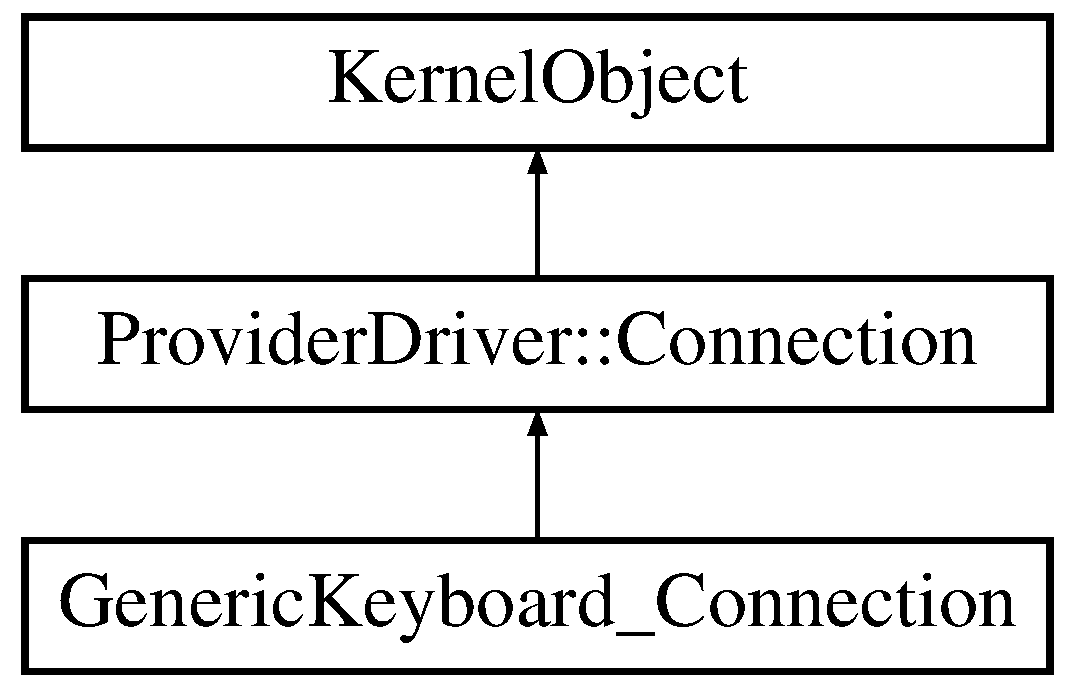
\includegraphics[height=3.000000cm]{class_generic_keyboard___connection}
\end{center}
\end{figure}
\subsection*{Public Member Functions}
\begin{DoxyCompactItemize}
\item 
\mbox{\Hypertarget{class_generic_keyboard___connection_a61982e1bf3f8943cec4eacf1fb136966}\label{class_generic_keyboard___connection_a61982e1bf3f8943cec4eacf1fb136966}} 
const char $\ast$ {\bfseries Get\+Class\+Name} (U\+Int32 level)
\item 
\mbox{\Hypertarget{class_generic_keyboard___connection_a4d81ad65ccc20afa0eb1ea4b6e5f67d6}\label{class_generic_keyboard___connection_a4d81ad65ccc20afa0eb1ea4b6e5f67d6}} 
{\bfseries Generic\+Keyboard\+\_\+\+Connection} (\hyperlink{class_generic_keyboard}{Generic\+Keyboard} $\ast$owner, \hyperlink{class_provider_driver_1_1_service}{Provider\+Driver\+::\+Service} $\ast$service, \hyperlink{class_ipc_endpoint}{Ipc\+Endpoint} $\ast$endpoint)
\end{DoxyCompactItemize}
\subsection*{Additional Inherited Members}


The documentation for this class was generated from the following file\+:\begin{DoxyCompactItemize}
\item 
Generic\+Keyboard.\+cpp\end{DoxyCompactItemize}

\hypertarget{class_generic_lock}{}\section{Generic\+Lock Class Reference}
\label{class_generic_lock}\index{Generic\+Lock@{Generic\+Lock}}
Inheritance diagram for Generic\+Lock\+:\begin{figure}[H]
\begin{center}
\leavevmode
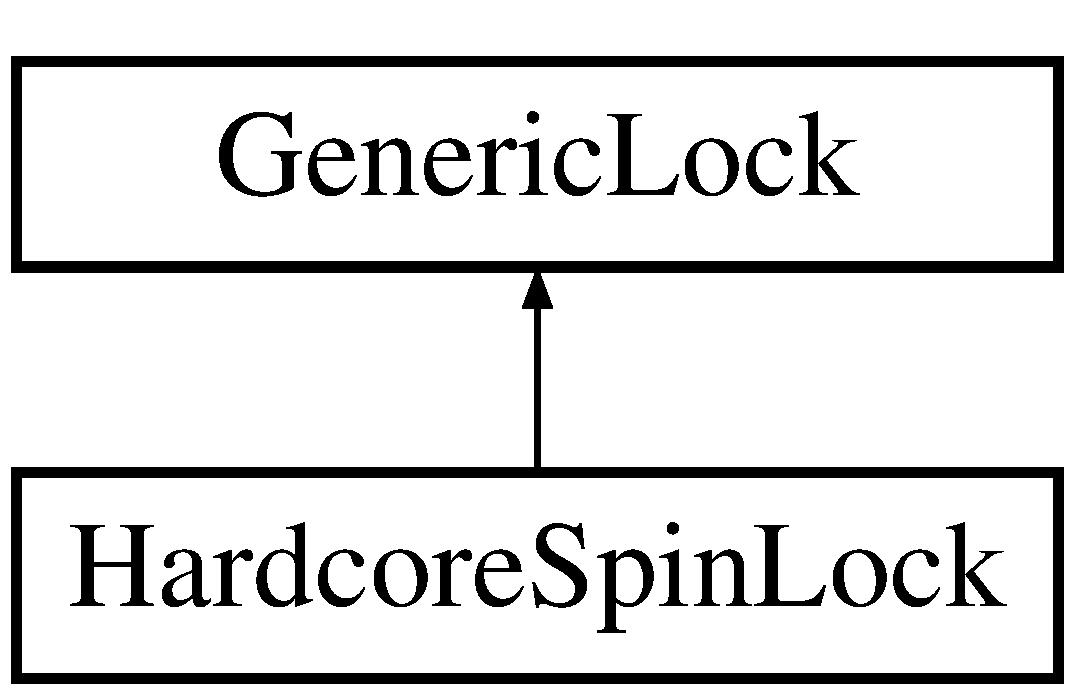
\includegraphics[height=2.000000cm]{class_generic_lock}
\end{center}
\end{figure}
\subsection*{Classes}
\begin{DoxyCompactItemize}
\item 
class \hyperlink{class_generic_lock_1_1_autolock}{Autolock}
\end{DoxyCompactItemize}
\subsection*{Public Member Functions}
\begin{DoxyCompactItemize}
\item 
\mbox{\Hypertarget{class_generic_lock_a78b911107ad38f5ea3db5f382e7100a5}\label{class_generic_lock_a78b911107ad38f5ea3db5f382e7100a5}} 
virtual void {\bfseries Lock} (void)
\item 
\mbox{\Hypertarget{class_generic_lock_aef3829188e15b0968c2fa14a8f754d5b}\label{class_generic_lock_aef3829188e15b0968c2fa14a8f754d5b}} 
virtual void {\bfseries Unlock} (void)
\item 
\mbox{\Hypertarget{class_generic_lock_ae0ed0d1aa6503437763c7eedd76eaa86}\label{class_generic_lock_ae0ed0d1aa6503437763c7eedd76eaa86}} 
virtual bool {\bfseries Holding} (void)=0
\end{DoxyCompactItemize}
\subsection*{Protected Member Functions}
\begin{DoxyCompactItemize}
\item 
\mbox{\Hypertarget{class_generic_lock_a6a310d2226a52bd5e5213b56becf2e1d}\label{class_generic_lock_a6a310d2226a52bd5e5213b56becf2e1d}} 
{\bfseries Generic\+Lock} (const char $\ast$lock\+Name)
\end{DoxyCompactItemize}
\subsection*{Protected Attributes}
\begin{DoxyCompactItemize}
\item 
\mbox{\Hypertarget{class_generic_lock_a699a610f530945caf6ebc9da0738bd3d}\label{class_generic_lock_a699a610f530945caf6ebc9da0738bd3d}} 
char $\ast$ {\bfseries \+\_\+name}
\item 
\mbox{\Hypertarget{class_generic_lock_aadc93550c44c1f710e3442205bf47c12}\label{class_generic_lock_aadc93550c44c1f710e3442205bf47c12}} 
\hyperlink{class_c_p_u}{C\+PU} $\ast$ {\bfseries \+\_\+cpu}
\item 
\mbox{\Hypertarget{class_generic_lock_a616f43d83b5396bf9efded878621764e}\label{class_generic_lock_a616f43d83b5396bf9efded878621764e}} 
Lock\+Int32 {\bfseries \+\_\+lock\+Stack} \mbox{[}10\mbox{]}
\end{DoxyCompactItemize}


The documentation for this class was generated from the following files\+:\begin{DoxyCompactItemize}
\item 
Locking.\+h\item 
Locking.\+cpp\end{DoxyCompactItemize}

\hypertarget{class_generic_mouse}{}\section{Generic\+Mouse Class Reference}
\label{class_generic_mouse}\index{Generic\+Mouse@{Generic\+Mouse}}
Inheritance diagram for Generic\+Mouse\+:\begin{figure}[H]
\begin{center}
\leavevmode
\includegraphics[height=5.000000cm]{class_generic_mouse}
\end{center}
\end{figure}
\subsection*{Public Member Functions}
\begin{DoxyCompactItemize}
\item 
\mbox{\Hypertarget{class_generic_mouse_a89c7ce7169444a492e8246ed4162839a}\label{class_generic_mouse_a89c7ce7169444a492e8246ed4162839a}} 
const char $\ast$ {\bfseries Get\+Class\+Name} (U\+Int32 level)
\item 
\mbox{\Hypertarget{class_generic_mouse_abc932bc5a5d13890cf4478689fb0353c}\label{class_generic_mouse_abc932bc5a5d13890cf4478689fb0353c}} 
{\bfseries Generic\+Mouse} (const char $\ast$name)
\item 
\mbox{\Hypertarget{class_generic_mouse_afe652111afa403e7407b91e50f1a77d6}\label{class_generic_mouse_afe652111afa403e7407b91e50f1a77d6}} 
bool {\bfseries Start} (\hyperlink{class_driver}{Driver} $\ast$parent)
\item 
\mbox{\Hypertarget{class_generic_mouse_a17a3923ab25e4826add22fc73b9b1e40}\label{class_generic_mouse_a17a3923ab25e4826add22fc73b9b1e40}} 
void {\bfseries Stop} (void)
\end{DoxyCompactItemize}
\subsection*{Protected Member Functions}
\begin{DoxyCompactItemize}
\item 
\mbox{\Hypertarget{class_generic_mouse_ae982497904804dc3586966dc44c087a5}\label{class_generic_mouse_ae982497904804dc3586966dc44c087a5}} 
void {\bfseries Move} (S\+Int32 x, S\+Int32 y)
\item 
\mbox{\Hypertarget{class_generic_mouse_adeeededabddd93d4c6349b98d3436e4c}\label{class_generic_mouse_adeeededabddd93d4c6349b98d3436e4c}} 
void {\bfseries Button} (U\+Int32 index, bool down)
\item 
\mbox{\Hypertarget{class_generic_mouse_a196dfde2263e2e8fb8efda7eae07fe67}\label{class_generic_mouse_a196dfde2263e2e8fb8efda7eae07fe67}} 
void {\bfseries Scroll} (S\+Int32 x, S\+Int32 y)
\item 
\mbox{\Hypertarget{class_generic_mouse_ab42c3bb04e2fd439f55c3d3a6a331051}\label{class_generic_mouse_ab42c3bb04e2fd439f55c3d3a6a331051}} 
\hyperlink{class_provider_driver_1_1_connection}{Connection} $\ast$ {\bfseries Connection\+Start} (\hyperlink{class_provider_driver_1_1_service}{Service} $\ast$service, \hyperlink{class_ipc_endpoint}{Ipc\+Endpoint} $\ast$endpoint)
\item 
\mbox{\Hypertarget{class_generic_mouse_a5a0092d02a7fbbf141e58d13e568640d}\label{class_generic_mouse_a5a0092d02a7fbbf141e58d13e568640d}} 
void {\bfseries Connection\+Receive} (\hyperlink{class_provider_driver_1_1_connection}{Connection} $\ast$connection, \hyperlink{class_kernel_buffer_memory}{Kernel\+Buffer\+Memory} $\ast$message)
\item 
\mbox{\Hypertarget{class_generic_mouse_a1bb452ac2b9e237ad60ddb377a514904}\label{class_generic_mouse_a1bb452ac2b9e237ad60ddb377a514904}} 
void {\bfseries Connection\+Stop} (\hyperlink{class_provider_driver_1_1_connection}{Connection} $\ast$connection)
\end{DoxyCompactItemize}
\subsection*{Protected Attributes}
\begin{DoxyCompactItemize}
\item 
\mbox{\Hypertarget{class_generic_mouse_a7c8d725fb20e262d2c7fb656a30684b4}\label{class_generic_mouse_a7c8d725fb20e262d2c7fb656a30684b4}} 
\hyperlink{class_runloop_thread}{Runloop\+Thread} $\ast$ {\bfseries \+\_\+thread}
\end{DoxyCompactItemize}
\subsection*{Private Member Functions}
\begin{DoxyCompactItemize}
\item 
\mbox{\Hypertarget{class_generic_mouse_aa1bff7fce968f5e27d5922b17e4a4541}\label{class_generic_mouse_aa1bff7fce968f5e27d5922b17e4a4541}} 
void {\bfseries Send\+Motion} (int x, int y, int type)
\end{DoxyCompactItemize}
\subsection*{Private Attributes}
\begin{DoxyCompactItemize}
\item 
\mbox{\Hypertarget{class_generic_mouse_a44d0165cb5da8ccb90acd9ea4a4419d1}\label{class_generic_mouse_a44d0165cb5da8ccb90acd9ea4a4419d1}} 
\hyperlink{class_provider_driver_1_1_service}{Service} $\ast$ {\bfseries \+\_\+service}
\item 
\mbox{\Hypertarget{class_generic_mouse_a53d0c2374616e0f4b1779fb35a725949}\label{class_generic_mouse_a53d0c2374616e0f4b1779fb35a725949}} 
int {\bfseries \+\_\+identifier\+Count}
\end{DoxyCompactItemize}
\subsection*{Additional Inherited Members}


The documentation for this class was generated from the following files\+:\begin{DoxyCompactItemize}
\item 
Generic\+Mouse.\+h\item 
Generic\+Mouse.\+cpp\end{DoxyCompactItemize}

\hypertarget{class_generic_mouse___connection}{}\section{Generic\+Mouse\+\_\+\+Connection Class Reference}
\label{class_generic_mouse___connection}\index{Generic\+Mouse\+\_\+\+Connection@{Generic\+Mouse\+\_\+\+Connection}}
Inheritance diagram for Generic\+Mouse\+\_\+\+Connection\+:\begin{figure}[H]
\begin{center}
\leavevmode
\includegraphics[height=3.000000cm]{class_generic_mouse___connection}
\end{center}
\end{figure}
\subsection*{Public Member Functions}
\begin{DoxyCompactItemize}
\item 
\mbox{\Hypertarget{class_generic_mouse___connection_ac83b2829d1695736efeba196801417e3}\label{class_generic_mouse___connection_ac83b2829d1695736efeba196801417e3}} 
const char $\ast$ {\bfseries Get\+Class\+Name} (U\+Int32 level)
\item 
\mbox{\Hypertarget{class_generic_mouse___connection_a60596cad7925599c80788e28f33c2584}\label{class_generic_mouse___connection_a60596cad7925599c80788e28f33c2584}} 
{\bfseries Generic\+Mouse\+\_\+\+Connection} (\hyperlink{class_generic_mouse}{Generic\+Mouse} $\ast$owner, \hyperlink{class_provider_driver_1_1_service}{Provider\+Driver\+::\+Service} $\ast$service, \hyperlink{class_ipc_endpoint}{Ipc\+Endpoint} $\ast$endpoint)
\end{DoxyCompactItemize}
\subsection*{Additional Inherited Members}


The documentation for this class was generated from the following file\+:\begin{DoxyCompactItemize}
\item 
Generic\+Mouse.\+cpp\end{DoxyCompactItemize}

\hypertarget{class_generic_provider}{}\section{Generic\+Provider Class Reference}
\label{class_generic_provider}\index{Generic\+Provider@{Generic\+Provider}}
Inheritance diagram for Generic\+Provider\+:\begin{figure}[H]
\begin{center}
\leavevmode
\includegraphics[height=1.388430cm]{class_generic_provider}
\end{center}
\end{figure}
\subsection*{Classes}
\begin{DoxyCompactItemize}
\item 
class \hyperlink{class_generic_provider_1_1_connection}{Connection}
\item 
class \hyperlink{class_generic_provider_1_1_factory}{Factory}
\item 
class \hyperlink{class_generic_provider_1_1_input}{Input}
\item 
class \hyperlink{class_generic_provider_1_1_input_connection}{Input\+Connection}
\item 
class \hyperlink{class_generic_provider_1_1_output_connection}{Output\+Connection}
\item 
class \hyperlink{class_generic_provider_1_1_service}{Service}
\item 
class \hyperlink{class_generic_provider_1_1_stash}{Stash}
\end{DoxyCompactItemize}
\subsection*{Public Member Functions}
\begin{DoxyCompactItemize}
\item 
\mbox{\Hypertarget{class_generic_provider_af3f64b26dedc39569ba00220d7e02f15}\label{class_generic_provider_af3f64b26dedc39569ba00220d7e02f15}} 
const char $\ast$ {\bfseries Get\+Class\+Name} (U\+Int32 level)
\item 
\mbox{\Hypertarget{class_generic_provider_a055659c50d30df73d358c9d89a58438d}\label{class_generic_provider_a055659c50d30df73d358c9d89a58438d}} 
{\bfseries Generic\+Provider} (\hyperlink{class_runloop_thread}{Runloop\+Thread} $\ast$runloop=0\+L)
\end{DoxyCompactItemize}
\subsection*{Protected Member Functions}
\begin{DoxyCompactItemize}
\item 
\mbox{\Hypertarget{class_generic_provider_afe4705c6685a0037b798ce06ca7d0831}\label{class_generic_provider_afe4705c6685a0037b798ce06ca7d0831}} 
void {\bfseries Launch} (\hyperlink{class_generic_provider_1_1_service}{Service} $\ast$service)
\item 
\mbox{\Hypertarget{class_generic_provider_abe6cac041cab50af23fffc2fe55c0e8c}\label{class_generic_provider_abe6cac041cab50af23fffc2fe55c0e8c}} 
void {\bfseries Kill} (\hyperlink{class_generic_provider_1_1_service}{Service} $\ast$service)
\item 
\mbox{\Hypertarget{class_generic_provider_a529c51b8ab4f6091009f807048d64fd6}\label{class_generic_provider_a529c51b8ab4f6091009f807048d64fd6}} 
virtual \hyperlink{class_generic_provider_1_1_input_connection}{Input\+Connection} $\ast$ {\bfseries Input\+Connection\+Start} (\hyperlink{class_kernel_string}{Kernel\+String} $\ast$name, \hyperlink{class_ipc_endpoint}{Ipc\+Endpoint} $\ast$connection)=0
\item 
\mbox{\Hypertarget{class_generic_provider_a512426f35c9f30ea0349ee7b8bd8a1c7}\label{class_generic_provider_a512426f35c9f30ea0349ee7b8bd8a1c7}} 
virtual void {\bfseries Input\+Connection\+Received} (\hyperlink{class_generic_provider_1_1_input_connection}{Input\+Connection} $\ast$connection, \hyperlink{class_kernel_buffer_memory}{Kernel\+Buffer\+Memory} $\ast$message)=0
\item 
\mbox{\Hypertarget{class_generic_provider_a9a20dd06d2274a7a14571de2c8f7c29b}\label{class_generic_provider_a9a20dd06d2274a7a14571de2c8f7c29b}} 
virtual void {\bfseries Input\+Connection\+End} (\hyperlink{class_generic_provider_1_1_input_connection}{Input\+Connection} $\ast$connection)=0
\item 
\mbox{\Hypertarget{class_generic_provider_ad5d5468ae38b686ad72833ac8b67bbfe}\label{class_generic_provider_ad5d5468ae38b686ad72833ac8b67bbfe}} 
virtual \hyperlink{class_generic_provider_1_1_output_connection}{Output\+Connection} $\ast$ {\bfseries Output\+Connection\+Start} (\hyperlink{class_generic_provider_1_1_service}{Service} $\ast$source, \hyperlink{class_ipc_endpoint}{Ipc\+Endpoint} $\ast$connection)=0
\item 
\mbox{\Hypertarget{class_generic_provider_a8c4b6eecd893d088376e3e83b9ed681a}\label{class_generic_provider_a8c4b6eecd893d088376e3e83b9ed681a}} 
virtual void {\bfseries Output\+Connection\+Message} (\hyperlink{class_generic_provider_1_1_output_connection}{Output\+Connection} $\ast$connection, \hyperlink{class_kernel_buffer_memory}{Kernel\+Buffer\+Memory} $\ast$message)=0
\item 
\mbox{\Hypertarget{class_generic_provider_a4a50940010e058da5113119d8eee2d2e}\label{class_generic_provider_a4a50940010e058da5113119d8eee2d2e}} 
virtual void {\bfseries Output\+Connection\+End} (\hyperlink{class_generic_provider_1_1_output_connection}{Output\+Connection} $\ast$old\+Connection)=0
\end{DoxyCompactItemize}
\subsection*{Protected Attributes}
\begin{DoxyCompactItemize}
\item 
\mbox{\Hypertarget{class_generic_provider_aedf53462a351ca88b8fd841f27394ee2}\label{class_generic_provider_aedf53462a351ca88b8fd841f27394ee2}} 
friend {\bfseries Generic\+Provider\+\_\+\+Thunk}
\item 
\mbox{\Hypertarget{class_generic_provider_a896e89cd9ab7ce816ea4b9f1dacf539a}\label{class_generic_provider_a896e89cd9ab7ce816ea4b9f1dacf539a}} 
\hyperlink{class_runloop_thread}{Runloop\+Thread} $\ast$ {\bfseries \+\_\+runloop}
\item 
\mbox{\Hypertarget{class_generic_provider_aa9627c4f6cef973632dad341f44c6bed}\label{class_generic_provider_aa9627c4f6cef973632dad341f44c6bed}} 
\hyperlink{class_kernel_dictionary}{Kernel\+Dictionary} $\ast$ {\bfseries \+\_\+inputs}
\item 
\mbox{\Hypertarget{class_generic_provider_a6e09a8d8f15b7ca6904f39e2321e0792}\label{class_generic_provider_a6e09a8d8f15b7ca6904f39e2321e0792}} 
\hyperlink{class_kernel_array}{Kernel\+Array} $\ast$ {\bfseries \+\_\+services}
\item 
\mbox{\Hypertarget{class_generic_provider_a311a7921fcdd59fa42f3ee2748353c61}\label{class_generic_provider_a311a7921fcdd59fa42f3ee2748353c61}} 
\hyperlink{class_kernel_array}{Kernel\+Array} $\ast$ {\bfseries \+\_\+connections}
\item 
\mbox{\Hypertarget{class_generic_provider_a06edbbc5a4d2a9428d42c85f0d05a456}\label{class_generic_provider_a06edbbc5a4d2a9428d42c85f0d05a456}} 
\hyperlink{class_ipc_service_proxy}{Ipc\+Service\+Proxy} $\ast$ {\bfseries \+\_\+service\+List}
\end{DoxyCompactItemize}
\subsection*{Additional Inherited Members}


The documentation for this class was generated from the following files\+:\begin{DoxyCompactItemize}
\item 
Provider.\+h\item 
Provider.\+cpp\end{DoxyCompactItemize}

\hypertarget{class_generic_provider___thunk}{}\section{Generic\+Provider\+\_\+\+Thunk Class Reference}
\label{class_generic_provider___thunk}\index{Generic\+Provider\+\_\+\+Thunk@{Generic\+Provider\+\_\+\+Thunk}}
\subsection*{Static Public Member Functions}
\begin{DoxyCompactItemize}
\item 
\mbox{\Hypertarget{class_generic_provider___thunk_a11c30597f6d697796056ed0858d7e880}\label{class_generic_provider___thunk_a11c30597f6d697796056ed0858d7e880}} 
static \hyperlink{class_generic_provider_1_1_input_connection}{Generic\+Provider\+::\+Input\+Connection} $\ast$ {\bfseries Input\+Connect} (\hyperlink{class_generic_provider}{Generic\+Provider} $\ast$provider, \hyperlink{class_kernel_string}{Kernel\+String} $\ast$name, \hyperlink{class_ipc_endpoint}{Ipc\+Endpoint} $\ast$connection)
\item 
\mbox{\Hypertarget{class_generic_provider___thunk_ad2286d701abe19d754fdd2e7e04883ca}\label{class_generic_provider___thunk_ad2286d701abe19d754fdd2e7e04883ca}} 
static void {\bfseries Input\+Message} (\hyperlink{class_generic_provider}{Generic\+Provider} $\ast$provider, \hyperlink{class_generic_provider_1_1_input_connection}{Generic\+Provider\+::\+Input\+Connection} $\ast$connection, \hyperlink{class_kernel_buffer_memory}{Kernel\+Buffer\+Memory} $\ast$message)
\item 
\mbox{\Hypertarget{class_generic_provider___thunk_a96aecd845f4b7c91630d9a307a045021}\label{class_generic_provider___thunk_a96aecd845f4b7c91630d9a307a045021}} 
static void {\bfseries Input\+Disconnect} (\hyperlink{class_generic_provider}{Generic\+Provider} $\ast$provider, \hyperlink{class_generic_provider_1_1_input_connection}{Generic\+Provider\+::\+Input\+Connection} $\ast$connection)
\item 
\mbox{\Hypertarget{class_generic_provider___thunk_aabbcdf1e3c9a0007281c51ddca7306fc}\label{class_generic_provider___thunk_aabbcdf1e3c9a0007281c51ddca7306fc}} 
static \hyperlink{class_generic_provider_1_1_output_connection}{Generic\+Provider\+::\+Output\+Connection} $\ast$ {\bfseries Output\+Connect} (\hyperlink{class_generic_provider}{Generic\+Provider} $\ast$provider, \hyperlink{class_generic_provider_1_1_service}{Generic\+Provider\+::\+Service} $\ast$source, \hyperlink{class_ipc_endpoint}{Ipc\+Endpoint} $\ast$connection)
\item 
\mbox{\Hypertarget{class_generic_provider___thunk_a6fe45b736110c95417c9c11402d89467}\label{class_generic_provider___thunk_a6fe45b736110c95417c9c11402d89467}} 
static void {\bfseries Output\+Message} (\hyperlink{class_generic_provider}{Generic\+Provider} $\ast$provider, \hyperlink{class_generic_provider_1_1_output_connection}{Generic\+Provider\+::\+Output\+Connection} $\ast$connection, \hyperlink{class_kernel_buffer_memory}{Kernel\+Buffer\+Memory} $\ast$message)
\item 
\mbox{\Hypertarget{class_generic_provider___thunk_a97a7b80984c8fa083544ab341178c98f}\label{class_generic_provider___thunk_a97a7b80984c8fa083544ab341178c98f}} 
static void {\bfseries Output\+Disconnect} (\hyperlink{class_generic_provider}{Generic\+Provider} $\ast$provider, \hyperlink{class_generic_provider_1_1_output_connection}{Generic\+Provider\+::\+Output\+Connection} $\ast$connection)
\item 
\mbox{\Hypertarget{class_generic_provider___thunk_a60ea7e3ebdc70baffd9c1593fc3ab005}\label{class_generic_provider___thunk_a60ea7e3ebdc70baffd9c1593fc3ab005}} 
static \hyperlink{class_kernel_dictionary}{Kernel\+Dictionary} $\ast$ {\bfseries Inputs} (\hyperlink{class_generic_provider}{Generic\+Provider} $\ast$provider)
\item 
\mbox{\Hypertarget{class_generic_provider___thunk_a7b451e574d9c4c3340f17e47235b2d4e}\label{class_generic_provider___thunk_a7b451e574d9c4c3340f17e47235b2d4e}} 
static \hyperlink{class_kernel_array}{Kernel\+Array} $\ast$ {\bfseries Connections} (\hyperlink{class_generic_provider}{Generic\+Provider} $\ast$provider)
\end{DoxyCompactItemize}


The documentation for this class was generated from the following file\+:\begin{DoxyCompactItemize}
\item 
Provider.\+cpp\end{DoxyCompactItemize}

\hypertarget{class_generic_video}{}\section{Generic\+Video Class Reference}
\label{class_generic_video}\index{Generic\+Video@{Generic\+Video}}
Inheritance diagram for Generic\+Video\+:\begin{figure}[H]
\begin{center}
\leavevmode
\includegraphics[height=5.000000cm]{class_generic_video}
\end{center}
\end{figure}
\subsection*{Classes}
\begin{DoxyCompactItemize}
\item 
struct \hyperlink{struct_generic_video_1_1_f_r_a_m_e_b_u_f_f_e_r}{F\+R\+A\+M\+E\+B\+U\+F\+F\+ER}
\item 
struct \hyperlink{struct_generic_video_1_1_m_o_d_e}{M\+O\+DE}
\end{DoxyCompactItemize}
\subsection*{Public Types}
\begin{DoxyCompactItemize}
\item 
\mbox{\Hypertarget{class_generic_video_a4c7668d1982087fd88cc45c1265d1016}\label{class_generic_video_a4c7668d1982087fd88cc45c1265d1016}} 
enum {\bfseries Match\+Level} \{ {\bfseries Match\+\_\+\+Specialised} = 10000, 
{\bfseries Match\+\_\+\+Default} = 1000, 
{\bfseries Match\+\_\+\+Backup} = 100
 \}
\end{DoxyCompactItemize}
\subsection*{Public Member Functions}
\begin{DoxyCompactItemize}
\item 
\mbox{\Hypertarget{class_generic_video_a3d88f7c2dbf327b2f5bf5ad0312cdc9b}\label{class_generic_video_a3d88f7c2dbf327b2f5bf5ad0312cdc9b}} 
const char $\ast$ {\bfseries Get\+Class\+Name} (U\+Int32 level)
\item 
\mbox{\Hypertarget{class_generic_video_a6d7ea217635188d4f4595b2552ffefbd}\label{class_generic_video_a6d7ea217635188d4f4595b2552ffefbd}} 
{\bfseries Generic\+Video} (const char $\ast$name)
\item 
\mbox{\Hypertarget{class_generic_video_a7f601466f4431a15ccbe5892e4f3a980}\label{class_generic_video_a7f601466f4431a15ccbe5892e4f3a980}} 
bool {\bfseries Start} (\hyperlink{class_driver}{Driver} $\ast$parent)
\item 
\mbox{\Hypertarget{class_generic_video_ac20f42bb81a05caaf029c40fd131e0ec}\label{class_generic_video_ac20f42bb81a05caaf029c40fd131e0ec}} 
void {\bfseries Stop} (void)
\end{DoxyCompactItemize}
\subsection*{Protected Types}
\begin{DoxyCompactItemize}
\item 
\mbox{\Hypertarget{class_generic_video_a3ff8211afd1d1e51e4bfbeb2e7f9e072}\label{class_generic_video_a3ff8211afd1d1e51e4bfbeb2e7f9e072}} 
enum {\bfseries T\+Y\+PE} \{ {\bfseries t\+Invalid}, 
{\bfseries t\+Graphical}, 
{\bfseries t\+Text}
 \}
\item 
\mbox{\Hypertarget{class_generic_video_a2af21b082d10a16e6e36a7bcb13f9691}\label{class_generic_video_a2af21b082d10a16e6e36a7bcb13f9691}} 
typedef void $\ast$ {\bfseries M\+O\+D\+E\+\_\+\+I\+D\+E\+N\+T\+I\+F\+I\+ER}
\end{DoxyCompactItemize}
\subsection*{Protected Member Functions}
\begin{DoxyCompactItemize}
\item 
\mbox{\Hypertarget{class_generic_video_a024f3e13dfe826a93d4d0ae0bd0f6794}\label{class_generic_video_a024f3e13dfe826a93d4d0ae0bd0f6794}} 
virtual int {\bfseries Get\+Port\+Count} (void)=0
\item 
\mbox{\Hypertarget{class_generic_video_aab4172455afed5a027bb0cafdce0afb1}\label{class_generic_video_aab4172455afed5a027bb0cafdce0afb1}} 
virtual int {\bfseries Get\+Modes} (int port, \hyperlink{struct_generic_video_1_1_m_o_d_e}{M\+O\+DE} $\ast$mode)=0
\item 
\mbox{\Hypertarget{class_generic_video_ad4f59851a53d5f54524aacd7ad8a3b45}\label{class_generic_video_ad4f59851a53d5f54524aacd7ad8a3b45}} 
virtual void {\bfseries Set\+Mode} (int port, M\+O\+D\+E\+\_\+\+I\+D\+E\+N\+T\+I\+F\+I\+ER mode)=0
\item 
\mbox{\Hypertarget{class_generic_video_a2d74e1db238df01cd93c0c49126c708d}\label{class_generic_video_a2d74e1db238df01cd93c0c49126c708d}} 
virtual M\+O\+D\+E\+\_\+\+I\+D\+E\+N\+T\+I\+F\+I\+ER {\bfseries Get\+Mode} (int port)=0
\item 
\mbox{\Hypertarget{class_generic_video_a86caece1005aff6d1db7bf6a786e7b64}\label{class_generic_video_a86caece1005aff6d1db7bf6a786e7b64}} 
void {\bfseries Update\+Port} (int index)
\item 
\mbox{\Hypertarget{class_generic_video_a9bab0c388d4d797c18aa68e057cb7cf6}\label{class_generic_video_a9bab0c388d4d797c18aa68e057cb7cf6}} 
virtual T\+Y\+PE {\bfseries Get\+Port\+Mode} (int index)=0
\item 
\mbox{\Hypertarget{class_generic_video_a6ec5a1ecef3f99c82fde3d71e7852781}\label{class_generic_video_a6ec5a1ecef3f99c82fde3d71e7852781}} 
virtual void {\bfseries Get\+Framebuffer} (int index, \hyperlink{struct_generic_video_1_1_f_r_a_m_e_b_u_f_f_e_r}{F\+R\+A\+M\+E\+B\+U\+F\+F\+ER} $\ast$info)=0
\item 
\mbox{\Hypertarget{class_generic_video_acf564daaf7cb4bda77d972997524dc62}\label{class_generic_video_acf564daaf7cb4bda77d972997524dc62}} 
virtual void {\bfseries Get\+Console} (int index, int $\ast$width, int $\ast$height, bool $\ast$colour, bool $\ast$cursor)=0
\item 
\mbox{\Hypertarget{class_generic_video_a743a1bef0b284e26b24edd5f5e8d1550}\label{class_generic_video_a743a1bef0b284e26b24edd5f5e8d1550}} 
virtual void {\bfseries Show\+Cursor} (int index, bool visible)=0
\item 
\mbox{\Hypertarget{class_generic_video_ad27368c06533fa4d5ede9363b8692a56}\label{class_generic_video_ad27368c06533fa4d5ede9363b8692a56}} 
virtual void {\bfseries Set\+Cursor} (int index, int x, int y)=0
\item 
\mbox{\Hypertarget{class_generic_video_a524776693a54935ce59bf0d949504bb1}\label{class_generic_video_a524776693a54935ce59bf0d949504bb1}} 
virtual void {\bfseries Set\+Colour} (int index, bool foreground, unsigned char r, unsigned char g, unsigned char b)=0
\item 
\mbox{\Hypertarget{class_generic_video_a0668a2e5722901419c0fd9249e235a12}\label{class_generic_video_a0668a2e5722901419c0fd9249e235a12}} 
virtual void {\bfseries Set\+Character} (int index, int x, int y, char c)=0
\item 
\mbox{\Hypertarget{class_generic_video_a6eba3c9ae7d4b98690ff0ae298befd4f}\label{class_generic_video_a6eba3c9ae7d4b98690ff0ae298befd4f}} 
virtual void {\bfseries Move\+Characters} (int index, int fromX, int fromY, int toX, int toY, int width, int height)=0
\end{DoxyCompactItemize}
\subsection*{Private Attributes}
\begin{DoxyCompactItemize}
\item 
\mbox{\Hypertarget{class_generic_video_a0e7c619087fdb7eb9b1f847c178fa7ad}\label{class_generic_video_a0e7c619087fdb7eb9b1f847c178fa7ad}} 
\hyperlink{class_kernel_dictionary}{Kernel\+Dictionary} $\ast$ {\bfseries \+\_\+ports}
\end{DoxyCompactItemize}
\subsection*{Additional Inherited Members}


The documentation for this class was generated from the following files\+:\begin{DoxyCompactItemize}
\item 
Generic\+Video.\+h\item 
Generic\+Video.\+cpp\end{DoxyCompactItemize}

\hypertarget{class_graphical_console_driver}{}\section{Graphical\+Console\+Driver Class Reference}
\label{class_graphical_console_driver}\index{Graphical\+Console\+Driver@{Graphical\+Console\+Driver}}
Inheritance diagram for Graphical\+Console\+Driver\+:\begin{figure}[H]
\begin{center}
\leavevmode
\includegraphics[height=2.000000cm]{class_graphical_console_driver}
\end{center}
\end{figure}
\subsection*{Public Member Functions}
\begin{DoxyCompactItemize}
\item 
\mbox{\Hypertarget{class_graphical_console_driver_a2e54aac1329dfd54696fcf5104810259}\label{class_graphical_console_driver_a2e54aac1329dfd54696fcf5104810259}} 
void {\bfseries Set\+Mode} (void $\ast$address, int width, int height, int pixel\+Span, int width\+Span, int depth)
\item 
\mbox{\Hypertarget{class_graphical_console_driver_a63cc9dea01f6dd077c571500d9e19fea}\label{class_graphical_console_driver_a63cc9dea01f6dd077c571500d9e19fea}} 
void {\bfseries Set} (char c, int x, int y, \hyperlink{class_console_driver_1_1_colour}{Colour} foreground=\hyperlink{class_console_driver_1_1_colour}{Colour}(255, 255, 255), \hyperlink{class_console_driver_1_1_colour}{Colour} background=\hyperlink{class_console_driver_1_1_colour}{Colour}(0, 0, 0))
\item 
\mbox{\Hypertarget{class_graphical_console_driver_afdfcf91a3df641a246d443f4f1437cf4}\label{class_graphical_console_driver_afdfcf91a3df641a246d443f4f1437cf4}} 
void {\bfseries Set\+Cursor} (int x, int y)
\item 
\mbox{\Hypertarget{class_graphical_console_driver_a49a19d5567c5370a995f9b021144d852}\label{class_graphical_console_driver_a49a19d5567c5370a995f9b021144d852}} 
void {\bfseries Get\+Cursor} (int $\ast$x, int $\ast$y)
\item 
\mbox{\Hypertarget{class_graphical_console_driver_a1c8cae5032b8567e64ba158544c751b5}\label{class_graphical_console_driver_a1c8cae5032b8567e64ba158544c751b5}} 
void {\bfseries Set\+Cursor\+Enabled} (bool enabled)
\item 
\mbox{\Hypertarget{class_graphical_console_driver_aa97a0ad0854e310207fc993b605224d8}\label{class_graphical_console_driver_aa97a0ad0854e310207fc993b605224d8}} 
int {\bfseries Width} (void)
\item 
\mbox{\Hypertarget{class_graphical_console_driver_a4442ccf1cdf30f4d16468ccd621298e5}\label{class_graphical_console_driver_a4442ccf1cdf30f4d16468ccd621298e5}} 
int {\bfseries Height} (void)
\item 
\mbox{\Hypertarget{class_graphical_console_driver_ac0f4c19da01bae81d3a54290cedbe5ce}\label{class_graphical_console_driver_ac0f4c19da01bae81d3a54290cedbe5ce}} 
void {\bfseries Clear} (int x, int y, int w, int h)
\item 
\mbox{\Hypertarget{class_graphical_console_driver_ae993d049898931292ded38d33f64354d}\label{class_graphical_console_driver_ae993d049898931292ded38d33f64354d}} 
void {\bfseries Copy} (int x\+From, int y\+From, int x\+To, int y\+To, int w, int h)
\end{DoxyCompactItemize}
\subsection*{Private Attributes}
\begin{DoxyCompactItemize}
\item 
\mbox{\Hypertarget{class_graphical_console_driver_a1ac384f819df9631698169a6e415619d}\label{class_graphical_console_driver_a1ac384f819df9631698169a6e415619d}} 
unsigned char $\ast$ {\bfseries \+\_\+buffer}
\item 
\mbox{\Hypertarget{class_graphical_console_driver_a86c44fe737f2b02079b265bc79e8f4d5}\label{class_graphical_console_driver_a86c44fe737f2b02079b265bc79e8f4d5}} 
int {\bfseries \+\_\+width}
\item 
\mbox{\Hypertarget{class_graphical_console_driver_a096769686cfbc0105b974764ce26914c}\label{class_graphical_console_driver_a096769686cfbc0105b974764ce26914c}} 
int {\bfseries \+\_\+height}
\item 
\mbox{\Hypertarget{class_graphical_console_driver_aefa1fcb29ead61934b858120a842709b}\label{class_graphical_console_driver_aefa1fcb29ead61934b858120a842709b}} 
int {\bfseries \+\_\+pixel\+Span}
\item 
\mbox{\Hypertarget{class_graphical_console_driver_ab95a4db949ab1cf30e7791f3a53ef84a}\label{class_graphical_console_driver_ab95a4db949ab1cf30e7791f3a53ef84a}} 
int {\bfseries \+\_\+width\+Span}
\item 
\mbox{\Hypertarget{class_graphical_console_driver_a130f94eb15b6984575dcf232286a8701}\label{class_graphical_console_driver_a130f94eb15b6984575dcf232286a8701}} 
int {\bfseries \+\_\+depth}
\item 
\mbox{\Hypertarget{class_graphical_console_driver_a5f29285731b4d8b2a185834e6264d775}\label{class_graphical_console_driver_a5f29285731b4d8b2a185834e6264d775}} 
int {\bfseries \+\_\+cursorX}
\item 
\mbox{\Hypertarget{class_graphical_console_driver_ad470a64bee743d331c954d08da26639d}\label{class_graphical_console_driver_ad470a64bee743d331c954d08da26639d}} 
int {\bfseries \+\_\+cursorY}
\item 
\mbox{\Hypertarget{class_graphical_console_driver_abd445916d14b4a5d430058ab496986ec}\label{class_graphical_console_driver_abd445916d14b4a5d430058ab496986ec}} 
bool {\bfseries \+\_\+cursor\+Enabled}
\item 
\mbox{\Hypertarget{class_graphical_console_driver_aab1afdf45a335c4ea3965a29ec8a101e}\label{class_graphical_console_driver_aab1afdf45a335c4ea3965a29ec8a101e}} 
void($\ast$ {\bfseries \+\_\+pixel\+Set} )(unsigned char $\ast$buffer, int width\+Span, int x, int y, \hyperlink{class_console_driver_1_1_colour}{Colour} colour)
\end{DoxyCompactItemize}


The documentation for this class was generated from the following files\+:\begin{DoxyCompactItemize}
\item 
Console.\+h\item 
Console.\+cpp\end{DoxyCompactItemize}

\hypertarget{class_growable_stack}{}\section{Growable\+Stack Class Reference}
\label{class_growable_stack}\index{Growable\+Stack@{Growable\+Stack}}
Inheritance diagram for Growable\+Stack\+:\begin{figure}[H]
\begin{center}
\leavevmode
\includegraphics[height=3.000000cm]{class_growable_stack}
\end{center}
\end{figure}
\subsection*{Public Member Functions}
\begin{DoxyCompactItemize}
\item 
\mbox{\Hypertarget{class_growable_stack_abce61b68dc37ec1599707fdfcc2d71c8}\label{class_growable_stack_abce61b68dc37ec1599707fdfcc2d71c8}} 
const char $\ast$ {\bfseries Get\+Class\+Name} (U\+Int32 level)
\item 
\mbox{\Hypertarget{class_growable_stack_a58153cde8bf389e48b0452a7f8d44687}\label{class_growable_stack_a58153cde8bf389e48b0452a7f8d44687}} 
{\bfseries Growable\+Stack} (\hyperlink{class_process}{Process} $\ast$process, U\+Int32 maximum\+Pages)
\item 
\mbox{\Hypertarget{class_growable_stack_ac65e7f4b6493793184c0a063fdec7ae3}\label{class_growable_stack_ac65e7f4b6493793184c0a063fdec7ae3}} 
void $\ast$ {\bfseries Stack\+Top} (void)
\item 
\mbox{\Hypertarget{class_growable_stack_a9db4cdc20c1c07ca26187df034f7298d}\label{class_growable_stack_a9db4cdc20c1c07ca26187df034f7298d}} 
\hyperlink{class_virtual_memory}{Virtual\+Memory} $\ast$ {\bfseries Map\+Into\+Kernel} (void)
\end{DoxyCompactItemize}
\subsection*{Protected Member Functions}
\begin{DoxyCompactItemize}
\item 
\mbox{\Hypertarget{class_growable_stack_a8f21f92acbb14fe4281c201b95d923de}\label{class_growable_stack_a8f21f92acbb14fe4281c201b95d923de}} 
void {\bfseries Handle\+Page\+Fault} (void $\ast$linear\+Address)
\end{DoxyCompactItemize}
\subsection*{Private Member Functions}
\begin{DoxyCompactItemize}
\item 
\mbox{\Hypertarget{class_growable_stack_ab5c4f65e9a4405e6171b8a2567e6f6e5}\label{class_growable_stack_ab5c4f65e9a4405e6171b8a2567e6f6e5}} 
Physical\+Pointer {\bfseries Get\+Address} (U\+Int32 offset)
\end{DoxyCompactItemize}
\subsection*{Private Attributes}
\begin{DoxyCompactItemize}
\item 
\mbox{\Hypertarget{class_growable_stack_acc455b20594b72ffa8f76786fc5ba113}\label{class_growable_stack_acc455b20594b72ffa8f76786fc5ba113}} 
friend {\bfseries Growable\+Stack\+Mapping}
\end{DoxyCompactItemize}
\subsection*{Additional Inherited Members}


The documentation for this class was generated from the following files\+:\begin{DoxyCompactItemize}
\item 
mem\+\_\+virtual.\+h\item 
mem\+\_\+virtual.\+cpp\end{DoxyCompactItemize}

\hypertarget{class_growable_stack_mapping}{}\section{Growable\+Stack\+Mapping Class Reference}
\label{class_growable_stack_mapping}\index{Growable\+Stack\+Mapping@{Growable\+Stack\+Mapping}}
Inheritance diagram for Growable\+Stack\+Mapping\+:\begin{figure}[H]
\begin{center}
\leavevmode
\includegraphics[height=3.000000cm]{class_growable_stack_mapping}
\end{center}
\end{figure}
\subsection*{Public Member Functions}
\begin{DoxyCompactItemize}
\item 
\mbox{\Hypertarget{class_growable_stack_mapping_a971ff1d54ebe4519e5d81eb23c450e15}\label{class_growable_stack_mapping_a971ff1d54ebe4519e5d81eb23c450e15}} 
const char $\ast$ {\bfseries Get\+Class\+Name} (U\+Int32 level)
\item 
\mbox{\Hypertarget{class_growable_stack_mapping_a0fd8a12a2711619ba496773ecc937729}\label{class_growable_stack_mapping_a0fd8a12a2711619ba496773ecc937729}} 
{\bfseries Growable\+Stack\+Mapping} (\hyperlink{class_growable_stack}{Growable\+Stack} $\ast$stack)
\end{DoxyCompactItemize}
\subsection*{Protected Member Functions}
\begin{DoxyCompactItemize}
\item 
\mbox{\Hypertarget{class_growable_stack_mapping_a8cc1fccf0d1533f25238d89535583e09}\label{class_growable_stack_mapping_a8cc1fccf0d1533f25238d89535583e09}} 
void {\bfseries Handle\+Page\+Fault} (void $\ast$linear\+Address)
\end{DoxyCompactItemize}
\subsection*{Private Attributes}
\begin{DoxyCompactItemize}
\item 
\mbox{\Hypertarget{class_growable_stack_mapping_a8c2f805c3b03ec78d2b377380fce6ca1}\label{class_growable_stack_mapping_a8c2f805c3b03ec78d2b377380fce6ca1}} 
\hyperlink{class_growable_stack}{Growable\+Stack} $\ast$ {\bfseries \+\_\+stack}
\end{DoxyCompactItemize}
\subsection*{Additional Inherited Members}


The documentation for this class was generated from the following file\+:\begin{DoxyCompactItemize}
\item 
mem\+\_\+virtual.\+cpp\end{DoxyCompactItemize}

\hypertarget{class_kernel_object___internal_1_1_handled_object}{}\section{Kernel\+Object\+\_\+\+Internal\+:\+:Handled\+Object Class Reference}
\label{class_kernel_object___internal_1_1_handled_object}\index{Kernel\+Object\+\_\+\+Internal\+::\+Handled\+Object@{Kernel\+Object\+\_\+\+Internal\+::\+Handled\+Object}}
Inheritance diagram for Kernel\+Object\+\_\+\+Internal\+:\+:Handled\+Object\+:\begin{figure}[H]
\begin{center}
\leavevmode
\includegraphics[height=2.000000cm]{class_kernel_object___internal_1_1_handled_object}
\end{center}
\end{figure}
\subsection*{Public Member Functions}
\begin{DoxyCompactItemize}
\item 
\mbox{\Hypertarget{class_kernel_object___internal_1_1_handled_object_abb1f87dd4f558cc863c0190781e7a833}\label{class_kernel_object___internal_1_1_handled_object_abb1f87dd4f558cc863c0190781e7a833}} 
const char $\ast$ {\bfseries Get\+Class\+Name} (U\+Int32 level)
\item 
\mbox{\Hypertarget{class_kernel_object___internal_1_1_handled_object_a81bf2b155b8c8c37d3957fbc2ce652d8}\label{class_kernel_object___internal_1_1_handled_object_a81bf2b155b8c8c37d3957fbc2ce652d8}} 
Handle {\bfseries Get\+Handle} (void)
\item 
\mbox{\Hypertarget{class_kernel_object___internal_1_1_handled_object_a6cbd10ce63492db268584cf2f4ee5550}\label{class_kernel_object___internal_1_1_handled_object_a6cbd10ce63492db268584cf2f4ee5550}} 
\hyperlink{class_kernel_object}{Kernel\+Object} $\ast$ {\bfseries Object} (void)
\item 
\mbox{\Hypertarget{class_kernel_object___internal_1_1_handled_object_a9b28bd635ae568d8ea706c7a1c832dc5}\label{class_kernel_object___internal_1_1_handled_object_a9b28bd635ae568d8ea706c7a1c832dc5}} 
bool {\bfseries User\+Add\+Ref} (void)
\item 
\mbox{\Hypertarget{class_kernel_object___internal_1_1_handled_object_a6187d669b52913f92050d603854a5656}\label{class_kernel_object___internal_1_1_handled_object_a6187d669b52913f92050d603854a5656}} 
bool {\bfseries User\+Release} (void)
\item 
\mbox{\Hypertarget{class_kernel_object___internal_1_1_handled_object_afb6b19db628f94bd94cc2db3c744c93d}\label{class_kernel_object___internal_1_1_handled_object_afb6b19db628f94bd94cc2db3c744c93d}} 
void {\bfseries Adjust\+Retain} (U\+Int32 adjust)
\item 
\mbox{\Hypertarget{class_kernel_object___internal_1_1_handled_object_a8595534a454e88e9fd645ebb8f9ebef1}\label{class_kernel_object___internal_1_1_handled_object_a8595534a454e88e9fd645ebb8f9ebef1}} 
{\bfseries Handled\+Object} (int handle, \hyperlink{class_kernel_object}{Kernel\+Object} $\ast$object, \hyperlink{classbicycle_1_1function}{bicycle\+::function}$<$ int(\hyperlink{class_kernel_object___internal_1_1_handled_object}{Handled\+Object} $\ast$)$>$ on\+Destroy, U\+Int32 initial\+User\+Retains)
\end{DoxyCompactItemize}
\subsection*{Private Attributes}
\begin{DoxyCompactItemize}
\item 
\mbox{\Hypertarget{class_kernel_object___internal_1_1_handled_object_af2ed8a56606b81ff99e248b12d6afc60}\label{class_kernel_object___internal_1_1_handled_object_af2ed8a56606b81ff99e248b12d6afc60}} 
Handle {\bfseries \+\_\+handle}
\item 
\mbox{\Hypertarget{class_kernel_object___internal_1_1_handled_object_a3390ae3115a327f5f3b0eff98d9736f6}\label{class_kernel_object___internal_1_1_handled_object_a3390ae3115a327f5f3b0eff98d9736f6}} 
\hyperlink{class_kernel_object}{Kernel\+Object} $\ast$ {\bfseries \+\_\+object}
\item 
\mbox{\Hypertarget{class_kernel_object___internal_1_1_handled_object_a6914d534c688d8f1f9a8024eca66cb58}\label{class_kernel_object___internal_1_1_handled_object_a6914d534c688d8f1f9a8024eca66cb58}} 
\hyperlink{class_kernel_object_1_1_destruction_watcher_handle}{Destruction\+Watcher\+Handle} $\ast$ {\bfseries \+\_\+watcher}
\item 
\mbox{\Hypertarget{class_kernel_object___internal_1_1_handled_object_a9e81627db5c4d453232489be54b93e80}\label{class_kernel_object___internal_1_1_handled_object_a9e81627db5c4d453232489be54b93e80}} 
U\+Int32 {\bfseries \+\_\+user\+Retain\+Count}
\end{DoxyCompactItemize}
\subsection*{Additional Inherited Members}


The documentation for this class was generated from the following file\+:\begin{DoxyCompactItemize}
\item 
Kernel\+Object.\+cpp\end{DoxyCompactItemize}

\hypertarget{class_startup___internal_1_1_handler}{}\section{Startup\+\_\+\+Internal\+:\+:Handler Class Reference}
\label{class_startup___internal_1_1_handler}\index{Startup\+\_\+\+Internal\+::\+Handler@{Startup\+\_\+\+Internal\+::\+Handler}}
Inheritance diagram for Startup\+\_\+\+Internal\+:\+:Handler\+:\begin{figure}[H]
\begin{center}
\leavevmode
\includegraphics[height=0.953192cm]{class_startup___internal_1_1_handler}
\end{center}
\end{figure}
\subsection*{Public Member Functions}
\begin{DoxyCompactItemize}
\item 
\mbox{\Hypertarget{class_startup___internal_1_1_handler_a8d10f849a4e9e97cc161beaa074b7b3c}\label{class_startup___internal_1_1_handler_a8d10f849a4e9e97cc161beaa074b7b3c}} 
{\bfseries Handler} (\hyperlink{classbicycle_1_1function}{bicycle\+::function}$<$ void(\hyperlink{class_startup___internal_1_1_handler}{Handler} $\ast$)$>$ updater)
\item 
\mbox{\Hypertarget{class_startup___internal_1_1_handler_a0f1676197cbb4c403e1caf56f94a5f21}\label{class_startup___internal_1_1_handler_a0f1676197cbb4c403e1caf56f94a5f21}} 
virtual void {\bfseries Found\+Input} (\hyperlink{class_kernel_object}{Kernel\+Object} $\ast$provider, \hyperlink{class_ipc_client}{Ipc\+Client} $\ast$client)=0
\item 
\mbox{\Hypertarget{class_startup___internal_1_1_handler_acd357ca0cbbd721227238c75f8a8e7aa}\label{class_startup___internal_1_1_handler_acd357ca0cbbd721227238c75f8a8e7aa}} 
virtual void {\bfseries Found\+Output} (\hyperlink{class_kernel_object}{Kernel\+Object} $\ast$provider, \hyperlink{class_ipc_service}{Ipc\+Service} $\ast$service)=0
\end{DoxyCompactItemize}
\subsection*{Protected Attributes}
\begin{DoxyCompactItemize}
\item 
\mbox{\Hypertarget{class_startup___internal_1_1_handler_a6568d82309ad571797abacbcc4ae7e9e}\label{class_startup___internal_1_1_handler_a6568d82309ad571797abacbcc4ae7e9e}} 
\hyperlink{classbicycle_1_1function}{bicycle\+::function}$<$ void(\hyperlink{class_startup___internal_1_1_handler}{Handler} $\ast$)$>$ {\bfseries \+\_\+updater}
\end{DoxyCompactItemize}


The documentation for this class was generated from the following file\+:\begin{DoxyCompactItemize}
\item 
Startup.\+cpp\end{DoxyCompactItemize}

\hypertarget{class_standard_p_c___internal_1_1_interrupts_1_1_handler_handle}{}\section{Standard\+P\+C\+\_\+\+Internal\+:\+:Interrupts\+:\+:Handler\+Handle Class Reference}
\label{class_standard_p_c___internal_1_1_interrupts_1_1_handler_handle}\index{Standard\+P\+C\+\_\+\+Internal\+::\+Interrupts\+::\+Handler\+Handle@{Standard\+P\+C\+\_\+\+Internal\+::\+Interrupts\+::\+Handler\+Handle}}
\subsection*{Public Member Functions}
\begin{DoxyCompactItemize}
\item 
\mbox{\Hypertarget{class_standard_p_c___internal_1_1_interrupts_1_1_handler_handle_aa0cd42d3b76365eec1915c1d5b85e67e}\label{class_standard_p_c___internal_1_1_interrupts_1_1_handler_handle_aa0cd42d3b76365eec1915c1d5b85e67e}} 
{\bfseries Handler\+Handle} (\hyperlink{class_standard_p_c___internal_1_1_interrupts_1_1_handler_handle}{Handler\+Handle} $\ast$$\ast$root, \hyperlink{classbicycle_1_1function}{Interrupt\+Handler\+Block} handler, U\+Int16 irq)
\end{DoxyCompactItemize}
\subsection*{Static Public Member Functions}
\begin{DoxyCompactItemize}
\item 
\mbox{\Hypertarget{class_standard_p_c___internal_1_1_interrupts_1_1_handler_handle_a4356b689bebad58bb05ba5e5f90d6d4c}\label{class_standard_p_c___internal_1_1_interrupts_1_1_handler_handle_a4356b689bebad58bb05ba5e5f90d6d4c}} 
static void {\bfseries Trigger} (\hyperlink{class_standard_p_c___internal_1_1_interrupts_1_1_handler_handle}{Handler\+Handle} $\ast$that, \hyperlink{struct_trap_frame}{Trap\+Frame} $\ast$frame)
\end{DoxyCompactItemize}
\subsection*{Public Attributes}
\begin{DoxyCompactItemize}
\item 
\mbox{\Hypertarget{class_standard_p_c___internal_1_1_interrupts_1_1_handler_handle_a72a595706d8182774873d0d4394de817}\label{class_standard_p_c___internal_1_1_interrupts_1_1_handler_handle_a72a595706d8182774873d0d4394de817}} 
U\+Int16 {\bfseries \+\_\+irq}
\end{DoxyCompactItemize}
\subsection*{Private Attributes}
\begin{DoxyCompactItemize}
\item 
\mbox{\Hypertarget{class_standard_p_c___internal_1_1_interrupts_1_1_handler_handle_a851e1bd553f6e2daee2aa40219d69140}\label{class_standard_p_c___internal_1_1_interrupts_1_1_handler_handle_a851e1bd553f6e2daee2aa40219d69140}} 
\hyperlink{class_standard_p_c___internal_1_1_interrupts_1_1_handler_handle}{Handler\+Handle} $\ast$$\ast$ {\bfseries \+\_\+root}
\item 
\mbox{\Hypertarget{class_standard_p_c___internal_1_1_interrupts_1_1_handler_handle_a37c1e708e90b2022058ebd4b308c4ebd}\label{class_standard_p_c___internal_1_1_interrupts_1_1_handler_handle_a37c1e708e90b2022058ebd4b308c4ebd}} 
\hyperlink{class_standard_p_c___internal_1_1_interrupts_1_1_handler_handle}{Handler\+Handle} $\ast$ {\bfseries \+\_\+last}
\item 
\mbox{\Hypertarget{class_standard_p_c___internal_1_1_interrupts_1_1_handler_handle_a575a50145ff91f9226edbb38987271eb}\label{class_standard_p_c___internal_1_1_interrupts_1_1_handler_handle_a575a50145ff91f9226edbb38987271eb}} 
\hyperlink{class_standard_p_c___internal_1_1_interrupts_1_1_handler_handle}{Handler\+Handle} $\ast$ {\bfseries \+\_\+next}
\item 
\mbox{\Hypertarget{class_standard_p_c___internal_1_1_interrupts_1_1_handler_handle_a7c0725c18ced9e5baf85f76dfb66ba1d}\label{class_standard_p_c___internal_1_1_interrupts_1_1_handler_handle_a7c0725c18ced9e5baf85f76dfb66ba1d}} 
\hyperlink{classbicycle_1_1function}{Interrupt\+Handler\+Block} {\bfseries \+\_\+handler}
\end{DoxyCompactItemize}


The documentation for this class was generated from the following file\+:\begin{DoxyCompactItemize}
\item 
Standard\+P\+C.\+cpp\end{DoxyCompactItemize}

\hypertarget{class_hardcore_spin_lock}{}\section{Hardcore\+Spin\+Lock Class Reference}
\label{class_hardcore_spin_lock}\index{Hardcore\+Spin\+Lock@{Hardcore\+Spin\+Lock}}
Inheritance diagram for Hardcore\+Spin\+Lock\+:\begin{figure}[H]
\begin{center}
\leavevmode
\includegraphics[height=2.000000cm]{class_hardcore_spin_lock}
\end{center}
\end{figure}
\subsection*{Public Member Functions}
\begin{DoxyCompactItemize}
\item 
\mbox{\Hypertarget{class_hardcore_spin_lock_aa185fc065ed475cca1663304ca913c8a}\label{class_hardcore_spin_lock_aa185fc065ed475cca1663304ca913c8a}} 
{\bfseries Hardcore\+Spin\+Lock} (const char $\ast$name)
\item 
\mbox{\Hypertarget{class_hardcore_spin_lock_a356eced86b643ed8005f7a444b1c08c0}\label{class_hardcore_spin_lock_a356eced86b643ed8005f7a444b1c08c0}} 
void {\bfseries Lock} (void)
\item 
\mbox{\Hypertarget{class_hardcore_spin_lock_a8247ac0425a17d728be8f56d740dcd08}\label{class_hardcore_spin_lock_a8247ac0425a17d728be8f56d740dcd08}} 
void {\bfseries Unlock} (void)
\item 
\mbox{\Hypertarget{class_hardcore_spin_lock_a81c726f719670690bd1e39785747c979}\label{class_hardcore_spin_lock_a81c726f719670690bd1e39785747c979}} 
bool {\bfseries Holding} (void)
\end{DoxyCompactItemize}
\subsection*{Private Attributes}
\begin{DoxyCompactItemize}
\item 
\mbox{\Hypertarget{class_hardcore_spin_lock_a9a65b2f64f0b2f2c38488f7643614616}\label{class_hardcore_spin_lock_a9a65b2f64f0b2f2c38488f7643614616}} 
Lock\+Int32 {\bfseries \+\_\+locked}
\item 
\mbox{\Hypertarget{class_hardcore_spin_lock_ae31bccb7b29faa3972e560fe91e947ec}\label{class_hardcore_spin_lock_ae31bccb7b29faa3972e560fe91e947ec}} 
Lock\+Int32 {\bfseries \+\_\+depth}
\end{DoxyCompactItemize}
\subsection*{Additional Inherited Members}


The documentation for this class was generated from the following files\+:\begin{DoxyCompactItemize}
\item 
Locking.\+h\item 
Locking.\+cpp\end{DoxyCompactItemize}

\hypertarget{class_hash_entry}{}\section{Hash\+Entry Class Reference}
\label{class_hash_entry}\index{Hash\+Entry@{Hash\+Entry}}
\subsection*{Public Member Functions}
\begin{DoxyCompactItemize}
\item 
\mbox{\Hypertarget{class_hash_entry_aa260f33a43f839975ed37c251b80ed4b}\label{class_hash_entry_aa260f33a43f839975ed37c251b80ed4b}} 
\hyperlink{class_entry}{Entry} $\ast$ {\bfseries Find} (\hyperlink{class_kernel_object}{Kernel\+Object} $\ast$key)
\item 
\mbox{\Hypertarget{class_hash_entry_ae893b9bbf0703e06408ac681671ed160}\label{class_hash_entry_ae893b9bbf0703e06408ac681671ed160}} 
void {\bfseries Set} (\hyperlink{class_kernel_object}{Kernel\+Object} $\ast$key, \hyperlink{class_kernel_object}{Kernel\+Object} $\ast$value)
\end{DoxyCompactItemize}
\subsection*{Public Attributes}
\begin{DoxyCompactItemize}
\item 
\mbox{\Hypertarget{class_hash_entry_a90d5921900705c1658b1d384ce9f0394}\label{class_hash_entry_a90d5921900705c1658b1d384ce9f0394}} 
\hyperlink{class_entry}{Entry} $\ast$ {\bfseries objects}
\end{DoxyCompactItemize}
\subsection*{Private Attributes}
\begin{DoxyCompactItemize}
\item 
\mbox{\Hypertarget{class_hash_entry_a0ae97dc4f2e30ad7b42c46a990b30b76}\label{class_hash_entry_a0ae97dc4f2e30ad7b42c46a990b30b76}} 
\hyperlink{class_entry}{Entry} $\ast$ {\bfseries end}
\end{DoxyCompactItemize}


The documentation for this class was generated from the following file\+:\begin{DoxyCompactItemize}
\item 
Collections.\+cpp\end{DoxyCompactItemize}

\hypertarget{class_image_loader}{}\section{Image\+Loader Class Reference}
\label{class_image_loader}\index{Image\+Loader@{Image\+Loader}}
Inheritance diagram for Image\+Loader\+:\begin{figure}[H]
\begin{center}
\leavevmode
\includegraphics[height=3.000000cm]{class_image_loader}
\end{center}
\end{figure}
\subsection*{Public Member Functions}
\begin{DoxyCompactItemize}
\item 
\mbox{\Hypertarget{class_image_loader_a90f79b71b80f026c0a0c8b8da07b9d23}\label{class_image_loader_a90f79b71b80f026c0a0c8b8da07b9d23}} 
const char $\ast$ {\bfseries Get\+Class\+Name} (U\+Int32 level)
\end{DoxyCompactItemize}
\subsection*{Protected Member Functions}
\begin{DoxyCompactItemize}
\item 
\mbox{\Hypertarget{class_image_loader_a5a21a1647a02f1db7af2582a46995254}\label{class_image_loader_a5a21a1647a02f1db7af2582a46995254}} 
\hyperlink{class_generic_provider_1_1_input_connection}{Input\+Connection} $\ast$ {\bfseries Input\+Connection\+Start} (\hyperlink{class_kernel_string}{Kernel\+String} $\ast$name, \hyperlink{class_ipc_endpoint}{Ipc\+Endpoint} $\ast$connection)
\item 
\mbox{\Hypertarget{class_image_loader_aa1e679360953cf9891dcacb4e7ecb3eb}\label{class_image_loader_aa1e679360953cf9891dcacb4e7ecb3eb}} 
void {\bfseries Input\+Connection\+Received} (\hyperlink{class_generic_provider_1_1_input_connection}{Input\+Connection} $\ast$connection, \hyperlink{class_kernel_buffer_memory}{Kernel\+Buffer\+Memory} $\ast$message)
\item 
\mbox{\Hypertarget{class_image_loader_a0d5902f1550af016f8c8bef14577a115}\label{class_image_loader_a0d5902f1550af016f8c8bef14577a115}} 
void {\bfseries Input\+Connection\+End} (\hyperlink{class_generic_provider_1_1_input_connection}{Input\+Connection} $\ast$connection)
\item 
\mbox{\Hypertarget{class_image_loader_a4f61980ed4221ded592c4297bc576c88}\label{class_image_loader_a4f61980ed4221ded592c4297bc576c88}} 
\hyperlink{class_generic_provider_1_1_output_connection}{Output\+Connection} $\ast$ {\bfseries Output\+Connection\+Start} (\hyperlink{class_generic_provider_1_1_service}{Service} $\ast$source, \hyperlink{class_ipc_endpoint}{Ipc\+Endpoint} $\ast$connection)
\item 
\mbox{\Hypertarget{class_image_loader_a023653de0385e1e33775a1f5464bbf21}\label{class_image_loader_a023653de0385e1e33775a1f5464bbf21}} 
void {\bfseries Output\+Connection\+Message} (\hyperlink{class_generic_provider_1_1_output_connection}{Output\+Connection} $\ast$connection, \hyperlink{class_kernel_buffer_memory}{Kernel\+Buffer\+Memory} $\ast$message)
\item 
\mbox{\Hypertarget{class_image_loader_a4ab1978124337eeb190582f1a454d348}\label{class_image_loader_a4ab1978124337eeb190582f1a454d348}} 
void {\bfseries Output\+Connection\+End} (\hyperlink{class_generic_provider_1_1_output_connection}{Output\+Connection} $\ast$old\+Connection)
\end{DoxyCompactItemize}
\subsection*{Private Member Functions}
\begin{DoxyCompactItemize}
\item 
\mbox{\Hypertarget{class_image_loader_a640b3940e97c44543443044079a9eb13}\label{class_image_loader_a640b3940e97c44543443044079a9eb13}} 
\hyperlink{class_generic_provider_1_1_input_connection}{Input\+Connection} $\ast$ {\bfseries Input} (void)
\end{DoxyCompactItemize}
\subsection*{Private Attributes}
\begin{DoxyCompactItemize}
\item 
\mbox{\Hypertarget{class_image_loader_a9d8d31cfd04da62114dc315e19682ffc}\label{class_image_loader_a9d8d31cfd04da62114dc315e19682ffc}} 
\hyperlink{class_interface_helper}{Interface\+Helper} $\ast$ {\bfseries \+\_\+tasks}
\item 
\mbox{\Hypertarget{class_image_loader_aaf0bbc6e3e14de1414caa7c2255c52ac}\label{class_image_loader_aaf0bbc6e3e14de1414caa7c2255c52ac}} 
\hyperlink{class_kernel_array}{Kernel\+Array} $\ast$ {\bfseries \+\_\+symbols}
\item 
\mbox{\Hypertarget{class_image_loader_a9f049d25ae5841fe9e7e10bb9d0cd374}\label{class_image_loader_a9f049d25ae5841fe9e7e10bb9d0cd374}} 
\hyperlink{class_kernel_array}{Kernel\+Array} $\ast$ {\bfseries \+\_\+segments}
\end{DoxyCompactItemize}
\subsection*{Additional Inherited Members}


The documentation for this class was generated from the following files\+:\begin{DoxyCompactItemize}
\item 
Image\+Loader.\+h\item 
Image\+Loader.\+cpp\end{DoxyCompactItemize}

\hypertarget{class_image_loader___segment}{}\section{Image\+Loader\+\_\+\+Segment Class Reference}
\label{class_image_loader___segment}\index{Image\+Loader\+\_\+\+Segment@{Image\+Loader\+\_\+\+Segment}}
Inheritance diagram for Image\+Loader\+\_\+\+Segment\+:\begin{figure}[H]
\begin{center}
\leavevmode
\includegraphics[height=2.000000cm]{class_image_loader___segment}
\end{center}
\end{figure}
\subsection*{Public Member Functions}
\begin{DoxyCompactItemize}
\item 
\mbox{\Hypertarget{class_image_loader___segment_ade18e83c203c412e785d973ced784d1c}\label{class_image_loader___segment_ade18e83c203c412e785d973ced784d1c}} 
const char $\ast$ {\bfseries Get\+Class\+Name} (U\+Int32 level)
\item 
\mbox{\Hypertarget{class_image_loader___segment_ae7ca816133fd5608d1f800caf1bfb10a}\label{class_image_loader___segment_ae7ca816133fd5608d1f800caf1bfb10a}} 
{\bfseries Image\+Loader\+\_\+\+Segment} (\hyperlink{struct_elf32___phdr}{Elf32\+\_\+\+Phdr} $\ast$header)
\item 
\mbox{\Hypertarget{class_image_loader___segment_af964b8a8102b0c8b67ea205dcb64288b}\label{class_image_loader___segment_af964b8a8102b0c8b67ea205dcb64288b}} 
U\+Int64 {\bfseries Virtual\+Address} (void)
\item 
\mbox{\Hypertarget{class_image_loader___segment_a4610f77d9120fe4a52d87b1fdb903b8d}\label{class_image_loader___segment_a4610f77d9120fe4a52d87b1fdb903b8d}} 
U\+Int64 {\bfseries Virtual\+Length} (void)
\item 
\mbox{\Hypertarget{class_image_loader___segment_a95638b6c6f6060fe84d41892cf1617e7}\label{class_image_loader___segment_a95638b6c6f6060fe84d41892cf1617e7}} 
U\+Int64 {\bfseries Write\+Flags} (void)
\item 
\mbox{\Hypertarget{class_image_loader___segment_a75db9682514d94b1c1307c3e094992f4}\label{class_image_loader___segment_a75db9682514d94b1c1307c3e094992f4}} 
U\+Int64 {\bfseries File\+Offset} (void)
\item 
\mbox{\Hypertarget{class_image_loader___segment_aa361c081bcef2b738d937a8a90609b6d}\label{class_image_loader___segment_aa361c081bcef2b738d937a8a90609b6d}} 
U\+Int64 {\bfseries File\+Length} (void)
\end{DoxyCompactItemize}
\subsection*{Private Attributes}
\begin{DoxyCompactItemize}
\item 
\mbox{\Hypertarget{class_image_loader___segment_ad83f34ab7ab6b0f073ddb3baa4f71b12}\label{class_image_loader___segment_ad83f34ab7ab6b0f073ddb3baa4f71b12}} 
U\+Int64 {\bfseries \+\_\+address}
\item 
\mbox{\Hypertarget{class_image_loader___segment_ace3b34c70ea09cd1f9fc26e5b8be0d3e}\label{class_image_loader___segment_ace3b34c70ea09cd1f9fc26e5b8be0d3e}} 
U\+Int64 {\bfseries \+\_\+length}
\item 
\mbox{\Hypertarget{class_image_loader___segment_a8a2bcb0fff7a42aa0840c1bc94a79ef2}\label{class_image_loader___segment_a8a2bcb0fff7a42aa0840c1bc94a79ef2}} 
U\+Int64 {\bfseries \+\_\+flags}
\item 
\mbox{\Hypertarget{class_image_loader___segment_a9517242b943c0f8cbba9e18a9fd663db}\label{class_image_loader___segment_a9517242b943c0f8cbba9e18a9fd663db}} 
U\+Int64 {\bfseries \+\_\+offset}
\item 
\mbox{\Hypertarget{class_image_loader___segment_a2b6f1b875ed8be014038d1fec95c83a2}\label{class_image_loader___segment_a2b6f1b875ed8be014038d1fec95c83a2}} 
U\+Int64 {\bfseries \+\_\+file\+Length}
\end{DoxyCompactItemize}
\subsection*{Additional Inherited Members}


The documentation for this class was generated from the following file\+:\begin{DoxyCompactItemize}
\item 
Image\+Loader.\+cpp\end{DoxyCompactItemize}

\hypertarget{class_image_loader___symbol}{}\section{Image\+Loader\+\_\+\+Symbol Class Reference}
\label{class_image_loader___symbol}\index{Image\+Loader\+\_\+\+Symbol@{Image\+Loader\+\_\+\+Symbol}}
Inheritance diagram for Image\+Loader\+\_\+\+Symbol\+:\begin{figure}[H]
\begin{center}
\leavevmode
\includegraphics[height=4.000000cm]{class_image_loader___symbol}
\end{center}
\end{figure}
\subsection*{Public Member Functions}
\begin{DoxyCompactItemize}
\item 
\mbox{\Hypertarget{class_image_loader___symbol_a8db8b1bb8b68a4e01b6958a732c1f42f}\label{class_image_loader___symbol_a8db8b1bb8b68a4e01b6958a732c1f42f}} 
const char $\ast$ {\bfseries Get\+Class\+Name} (U\+Int32 level)
\item 
\mbox{\Hypertarget{class_image_loader___symbol_a987681bd76930d8f7c520d8281469e36}\label{class_image_loader___symbol_a987681bd76930d8f7c520d8281469e36}} 
virtual U\+Int64 {\bfseries Address} (void)=0
\item 
\mbox{\Hypertarget{class_image_loader___symbol_a443e7ff4ca62518a6ad9308cef438e0a}\label{class_image_loader___symbol_a443e7ff4ca62518a6ad9308cef438e0a}} 
virtual void {\bfseries Encode} (Flat\+Dictionary $\ast$output)=0
\end{DoxyCompactItemize}
\subsection*{Additional Inherited Members}


The documentation for this class was generated from the following file\+:\begin{DoxyCompactItemize}
\item 
Image\+Loader.\+cpp\end{DoxyCompactItemize}

\hypertarget{class_image_loader___symbol___entry_point}{}\section{Image\+Loader\+\_\+\+Symbol\+\_\+\+Entry\+Point Class Reference}
\label{class_image_loader___symbol___entry_point}\index{Image\+Loader\+\_\+\+Symbol\+\_\+\+Entry\+Point@{Image\+Loader\+\_\+\+Symbol\+\_\+\+Entry\+Point}}
Inheritance diagram for Image\+Loader\+\_\+\+Symbol\+\_\+\+Entry\+Point\+:\begin{figure}[H]
\begin{center}
\leavevmode
\includegraphics[height=4.000000cm]{class_image_loader___symbol___entry_point}
\end{center}
\end{figure}
\subsection*{Public Member Functions}
\begin{DoxyCompactItemize}
\item 
\mbox{\Hypertarget{class_image_loader___symbol___entry_point_aabd13b5bdf106c5b76257b86bda80ef9}\label{class_image_loader___symbol___entry_point_aabd13b5bdf106c5b76257b86bda80ef9}} 
const char $\ast$ {\bfseries Get\+Class\+Name} (U\+Int32 level)
\item 
\mbox{\Hypertarget{class_image_loader___symbol___entry_point_a7aef7b9543ebecdd3247d7569a4cf09c}\label{class_image_loader___symbol___entry_point_a7aef7b9543ebecdd3247d7569a4cf09c}} 
{\bfseries Image\+Loader\+\_\+\+Symbol\+\_\+\+Entry\+Point} (U\+Int64 address, \hyperlink{class_kernel_string}{Kernel\+String} $\ast$name)
\item 
\mbox{\Hypertarget{class_image_loader___symbol___entry_point_a3c3e934d2241d7c44013c2fa3938ecc4}\label{class_image_loader___symbol___entry_point_a3c3e934d2241d7c44013c2fa3938ecc4}} 
void {\bfseries Encode} (Flat\+Dictionary $\ast$output)
\end{DoxyCompactItemize}
\subsection*{Private Attributes}
\begin{DoxyCompactItemize}
\item 
\mbox{\Hypertarget{class_image_loader___symbol___entry_point_a9139121e368b8bd58a7b16cd1d4caefc}\label{class_image_loader___symbol___entry_point_a9139121e368b8bd58a7b16cd1d4caefc}} 
\hyperlink{class_kernel_string}{Kernel\+String} $\ast$ {\bfseries \+\_\+name}
\end{DoxyCompactItemize}
\subsection*{Additional Inherited Members}


The documentation for this class was generated from the following file\+:\begin{DoxyCompactItemize}
\item 
Image\+Loader.\+cpp\end{DoxyCompactItemize}

\hypertarget{class_image_loader___symbol___main}{}\section{Image\+Loader\+\_\+\+Symbol\+\_\+\+Main Class Reference}
\label{class_image_loader___symbol___main}\index{Image\+Loader\+\_\+\+Symbol\+\_\+\+Main@{Image\+Loader\+\_\+\+Symbol\+\_\+\+Main}}
Inheritance diagram for Image\+Loader\+\_\+\+Symbol\+\_\+\+Main\+:\begin{figure}[H]
\begin{center}
\leavevmode
\includegraphics[height=4.000000cm]{class_image_loader___symbol___main}
\end{center}
\end{figure}
\subsection*{Public Member Functions}
\begin{DoxyCompactItemize}
\item 
\mbox{\Hypertarget{class_image_loader___symbol___main_a15ff87a18a8f0a877c46d8c93aa09ac5}\label{class_image_loader___symbol___main_a15ff87a18a8f0a877c46d8c93aa09ac5}} 
const char $\ast$ {\bfseries Get\+Class\+Name} (U\+Int32 level)
\item 
\mbox{\Hypertarget{class_image_loader___symbol___main_a6bcabf879b16c29de14b618fb47a53ed}\label{class_image_loader___symbol___main_a6bcabf879b16c29de14b618fb47a53ed}} 
{\bfseries Image\+Loader\+\_\+\+Symbol\+\_\+\+Main} (U\+Int64 main)
\item 
\mbox{\Hypertarget{class_image_loader___symbol___main_ae7161c654c87b705bdecc2d9aa5953d6}\label{class_image_loader___symbol___main_ae7161c654c87b705bdecc2d9aa5953d6}} 
U\+Int64 {\bfseries Address} (void)
\item 
\mbox{\Hypertarget{class_image_loader___symbol___main_a4fb54a0fe8904ed2a32a7970dfe9dfef}\label{class_image_loader___symbol___main_a4fb54a0fe8904ed2a32a7970dfe9dfef}} 
void {\bfseries Encode} (Flat\+Dictionary $\ast$output)
\end{DoxyCompactItemize}
\subsection*{Private Attributes}
\begin{DoxyCompactItemize}
\item 
\mbox{\Hypertarget{class_image_loader___symbol___main_a494bb3eafd2f1a6ce9b5b46e5aaaa583}\label{class_image_loader___symbol___main_a494bb3eafd2f1a6ce9b5b46e5aaaa583}} 
U\+Int64 {\bfseries \+\_\+main}
\end{DoxyCompactItemize}
\subsection*{Additional Inherited Members}


The documentation for this class was generated from the following file\+:\begin{DoxyCompactItemize}
\item 
Image\+Loader.\+cpp\end{DoxyCompactItemize}

\hypertarget{class_convenient_sink___internal_1_1_input}{}\section{Convenient\+Sink\+\_\+\+Internal\+:\+:Input Class Reference}
\label{class_convenient_sink___internal_1_1_input}\index{Convenient\+Sink\+\_\+\+Internal\+::\+Input@{Convenient\+Sink\+\_\+\+Internal\+::\+Input}}
Inheritance diagram for Convenient\+Sink\+\_\+\+Internal\+:\+:Input\+:\begin{figure}[H]
\begin{center}
\leavevmode
\includegraphics[height=4.000000cm]{class_convenient_sink___internal_1_1_input}
\end{center}
\end{figure}
\subsection*{Public Member Functions}
\begin{DoxyCompactItemize}
\item 
\mbox{\Hypertarget{class_convenient_sink___internal_1_1_input_a0d905e4ffc38d483d1a98ac335d1ba55}\label{class_convenient_sink___internal_1_1_input_a0d905e4ffc38d483d1a98ac335d1ba55}} 
{\bfseries Input} (\hyperlink{class_generic_provider}{Generic\+Provider} $\ast$owner, \hyperlink{class_kernel_string}{Kernel\+String} $\ast$name, \hyperlink{classbicycle_1_1function}{bicycle\+::function}$<$ bool(\hyperlink{class_ipc_endpoint}{Ipc\+Endpoint} $\ast$)$>$ connection\+Handler)
\item 
\mbox{\Hypertarget{class_convenient_sink___internal_1_1_input_a031cd58b07adabd8e6f1741080215e94}\label{class_convenient_sink___internal_1_1_input_a031cd58b07adabd8e6f1741080215e94}} 
bool {\bfseries Should\+Connect} (\hyperlink{class_ipc_endpoint}{Ipc\+Endpoint} $\ast$endpoint)
\end{DoxyCompactItemize}
\subsection*{Private Attributes}
\begin{DoxyCompactItemize}
\item 
\mbox{\Hypertarget{class_convenient_sink___internal_1_1_input_a233ca94cb4012e4e6b4aed6afd9aed6c}\label{class_convenient_sink___internal_1_1_input_a233ca94cb4012e4e6b4aed6afd9aed6c}} 
\hyperlink{classbicycle_1_1function}{bicycle\+::function}$<$ bool(\hyperlink{class_ipc_endpoint}{Ipc\+Endpoint} $\ast$)$>$ {\bfseries \+\_\+connection\+Handler}
\end{DoxyCompactItemize}
\subsection*{Additional Inherited Members}


The documentation for this class was generated from the following file\+:\begin{DoxyCompactItemize}
\item 
Convenient\+Sink.\+cpp\end{DoxyCompactItemize}

\hypertarget{class_generic_provider_1_1_input}{}\section{Generic\+Provider\+:\+:Input Class Reference}
\label{class_generic_provider_1_1_input}\index{Generic\+Provider\+::\+Input@{Generic\+Provider\+::\+Input}}
Inheritance diagram for Generic\+Provider\+:\+:Input\+:\begin{figure}[H]
\begin{center}
\leavevmode
\includegraphics[height=4.000000cm]{class_generic_provider_1_1_input}
\end{center}
\end{figure}
\subsection*{Public Member Functions}
\begin{DoxyCompactItemize}
\item 
\mbox{\Hypertarget{class_generic_provider_1_1_input_ada4c804a620739200b092c515de715cf}\label{class_generic_provider_1_1_input_ada4c804a620739200b092c515de715cf}} 
const char $\ast$ {\bfseries Get\+Class\+Name} (U\+Int32 level)
\item 
\mbox{\Hypertarget{class_generic_provider_1_1_input_ad57336e411b51000ab32aa6f20278b60}\label{class_generic_provider_1_1_input_ad57336e411b51000ab32aa6f20278b60}} 
{\bfseries Input} (\hyperlink{class_generic_provider}{Generic\+Provider} $\ast$owner, \hyperlink{class_kernel_string}{Kernel\+String} $\ast$name)
\item 
\mbox{\Hypertarget{class_generic_provider_1_1_input_a972ad0d779ab00ba19e05258b690ef07}\label{class_generic_provider_1_1_input_a972ad0d779ab00ba19e05258b690ef07}} 
void {\bfseries Connect} (\hyperlink{class_ipc_service}{Ipc\+Service} $\ast$service)
\item 
\mbox{\Hypertarget{class_generic_provider_1_1_input_a1c7cd203e8ab72138e7b45270955ccb5}\label{class_generic_provider_1_1_input_a1c7cd203e8ab72138e7b45270955ccb5}} 
void {\bfseries Disconnect} (void)
\end{DoxyCompactItemize}
\subsection*{Protected Member Functions}
\begin{DoxyCompactItemize}
\item 
\mbox{\Hypertarget{class_generic_provider_1_1_input_abbdae40ca57e0b9ac93caec0ff9f811c}\label{class_generic_provider_1_1_input_abbdae40ca57e0b9ac93caec0ff9f811c}} 
\hyperlink{class_generic_provider}{Generic\+Provider} $\ast$ {\bfseries Owner} (void)
\end{DoxyCompactItemize}
\subsection*{Private Member Functions}
\begin{DoxyCompactItemize}
\item 
\mbox{\Hypertarget{class_generic_provider_1_1_input_a865caf97ec99e4272f1eb1bb7472ae84}\label{class_generic_provider_1_1_input_a865caf97ec99e4272f1eb1bb7472ae84}} 
void {\bfseries Do\+Disconnect} (void)
\end{DoxyCompactItemize}
\subsection*{Private Attributes}
\begin{DoxyCompactItemize}
\item 
\mbox{\Hypertarget{class_generic_provider_1_1_input_a325fa3b2b9ad99a5353e7aa28ba63689}\label{class_generic_provider_1_1_input_a325fa3b2b9ad99a5353e7aa28ba63689}} 
\hyperlink{class_generic_provider}{Generic\+Provider} $\ast$ {\bfseries \+\_\+owner}
\item 
\mbox{\Hypertarget{class_generic_provider_1_1_input_a3b3b207c304cad64c2e9befc5cac88e8}\label{class_generic_provider_1_1_input_a3b3b207c304cad64c2e9befc5cac88e8}} 
\hyperlink{class_generic_provider_1_1_input_connection}{Input\+Connection} $\ast$ {\bfseries \+\_\+connection}
\end{DoxyCompactItemize}
\subsection*{Additional Inherited Members}


The documentation for this class was generated from the following files\+:\begin{DoxyCompactItemize}
\item 
Provider.\+h\item 
Provider.\+cpp\end{DoxyCompactItemize}

\hypertarget{class_generic_provider_1_1_input_connection}{}\section{Generic\+Provider\+:\+:Input\+Connection Class Reference}
\label{class_generic_provider_1_1_input_connection}\index{Generic\+Provider\+::\+Input\+Connection@{Generic\+Provider\+::\+Input\+Connection}}
Inheritance diagram for Generic\+Provider\+:\+:Input\+Connection\+:\begin{figure}[H]
\begin{center}
\leavevmode
\includegraphics[height=3.000000cm]{class_generic_provider_1_1_input_connection}
\end{center}
\end{figure}
\subsection*{Public Member Functions}
\begin{DoxyCompactItemize}
\item 
\mbox{\Hypertarget{class_generic_provider_1_1_input_connection_ae97f413cf0d14f7b2fe570f36aba39b3}\label{class_generic_provider_1_1_input_connection_ae97f413cf0d14f7b2fe570f36aba39b3}} 
const char $\ast$ {\bfseries Get\+Class\+Name} (U\+Int32 level)
\item 
\mbox{\Hypertarget{class_generic_provider_1_1_input_connection_a604b9b4e332f6adb4fc5983df93e97ed}\label{class_generic_provider_1_1_input_connection_a604b9b4e332f6adb4fc5983df93e97ed}} 
{\bfseries Input\+Connection} (\hyperlink{class_generic_provider}{Generic\+Provider} $\ast$owner, \hyperlink{class_kernel_string}{Kernel\+String} $\ast$input, \hyperlink{class_ipc_endpoint}{Ipc\+Endpoint} $\ast$connection)
\item 
\mbox{\Hypertarget{class_generic_provider_1_1_input_connection_a3e4f0520957781b0c064819490eabe34}\label{class_generic_provider_1_1_input_connection_a3e4f0520957781b0c064819490eabe34}} 
\hyperlink{class_kernel_string}{Kernel\+String} $\ast$ {\bfseries Source} (void)
\end{DoxyCompactItemize}
\subsection*{Private Attributes}
\begin{DoxyCompactItemize}
\item 
\mbox{\Hypertarget{class_generic_provider_1_1_input_connection_a616ddff8551c141a24cc122d1822b1b2}\label{class_generic_provider_1_1_input_connection_a616ddff8551c141a24cc122d1822b1b2}} 
\hyperlink{class_kernel_string}{Kernel\+String} $\ast$ {\bfseries \+\_\+source}
\end{DoxyCompactItemize}
\subsection*{Additional Inherited Members}


The documentation for this class was generated from the following files\+:\begin{DoxyCompactItemize}
\item 
Provider.\+h\item 
Provider.\+cpp\end{DoxyCompactItemize}

\hypertarget{class_i_s_o9660_driver_1_1_interface___file___output}{}\section{I\+S\+O9660\+Driver\+:\+:Interface\+\_\+\+File\+\_\+\+Output Class Reference}
\label{class_i_s_o9660_driver_1_1_interface___file___output}\index{I\+S\+O9660\+Driver\+::\+Interface\+\_\+\+File\+\_\+\+Output@{I\+S\+O9660\+Driver\+::\+Interface\+\_\+\+File\+\_\+\+Output}}
Inheritance diagram for I\+S\+O9660\+Driver\+:\+:Interface\+\_\+\+File\+\_\+\+Output\+:\begin{figure}[H]
\begin{center}
\leavevmode
\includegraphics[height=4.000000cm]{class_i_s_o9660_driver_1_1_interface___file___output}
\end{center}
\end{figure}
\subsection*{Public Member Functions}
\begin{DoxyCompactItemize}
\item 
\mbox{\Hypertarget{class_i_s_o9660_driver_1_1_interface___file___output_a126c81346394299cf8c02965d0fd70c9}\label{class_i_s_o9660_driver_1_1_interface___file___output_a126c81346394299cf8c02965d0fd70c9}} 
const char $\ast$ {\bfseries Get\+Class\+Name} (U\+Int32 level)
\item 
\mbox{\Hypertarget{class_i_s_o9660_driver_1_1_interface___file___output_a6e9c7ef46302d08628c9fcdb5adc06e2}\label{class_i_s_o9660_driver_1_1_interface___file___output_a6e9c7ef46302d08628c9fcdb5adc06e2}} 
{\bfseries Interface\+\_\+\+File\+\_\+\+Output} (\hyperlink{class_file_system___i_s_o9660}{File\+System\+\_\+\+I\+S\+O9660} $\ast$owner, \hyperlink{class_generic_provider_1_1_service}{Generic\+Provider\+::\+Service} $\ast$service, \hyperlink{class_ipc_endpoint}{Ipc\+Endpoint} $\ast$endpoint)
\item 
\mbox{\Hypertarget{class_i_s_o9660_driver_1_1_interface___file___output_a4d9050fa4df5f84b93c99d5d5e264990}\label{class_i_s_o9660_driver_1_1_interface___file___output_a4d9050fa4df5f84b93c99d5d5e264990}} 
U\+Int32 {\bfseries Open} (\hyperlink{class_i_s_o9660_driver_1_1_file_entry}{File\+Entry} $\ast$file)
\item 
\mbox{\Hypertarget{class_i_s_o9660_driver_1_1_interface___file___output_a55045f95f559b3aa96879e95d18220b0}\label{class_i_s_o9660_driver_1_1_interface___file___output_a55045f95f559b3aa96879e95d18220b0}} 
void {\bfseries Close} (U\+Int32 file\+Handle)
\item 
\mbox{\Hypertarget{class_i_s_o9660_driver_1_1_interface___file___output_aa261680b427fb2718e3ea193c6d6aeec}\label{class_i_s_o9660_driver_1_1_interface___file___output_aa261680b427fb2718e3ea193c6d6aeec}} 
\hyperlink{class_i_s_o9660_driver_1_1_file_entry}{File\+Entry} $\ast$ {\bfseries File\+For\+Handle} (U\+Int32 file\+Handle)
\end{DoxyCompactItemize}
\subsection*{Private Attributes}
\begin{DoxyCompactItemize}
\item 
\mbox{\Hypertarget{class_i_s_o9660_driver_1_1_interface___file___output_a9ed6bfa64925f57618fc70f2a3276447}\label{class_i_s_o9660_driver_1_1_interface___file___output_a9ed6bfa64925f57618fc70f2a3276447}} 
\hyperlink{class_kernel_dictionary}{Kernel\+Dictionary} $\ast$ {\bfseries \+\_\+handles}
\item 
\mbox{\Hypertarget{class_i_s_o9660_driver_1_1_interface___file___output_a958ccfc7bb1c36033395ea466d565f6e}\label{class_i_s_o9660_driver_1_1_interface___file___output_a958ccfc7bb1c36033395ea466d565f6e}} 
U\+Int32 {\bfseries \+\_\+handle\+Count}
\end{DoxyCompactItemize}
\subsection*{Additional Inherited Members}


The documentation for this class was generated from the following file\+:\begin{DoxyCompactItemize}
\item 
fs\+\_\+iso9660.\+cpp\end{DoxyCompactItemize}

\hypertarget{class_interface_helper}{}\section{Interface\+Helper Class Reference}
\label{class_interface_helper}\index{Interface\+Helper@{Interface\+Helper}}
Inheritance diagram for Interface\+Helper\+:\begin{figure}[H]
\begin{center}
\leavevmode
\includegraphics[height=2.000000cm]{class_interface_helper}
\end{center}
\end{figure}
\subsection*{Public Member Functions}
\begin{DoxyCompactItemize}
\item 
\mbox{\Hypertarget{class_interface_helper_ab0d93a8b33030d4612311d48cd5dded7}\label{class_interface_helper_ab0d93a8b33030d4612311d48cd5dded7}} 
const char $\ast$ {\bfseries Get\+Class\+Name} (U\+Int32 level)
\item 
\mbox{\Hypertarget{class_interface_helper_acd3fda4f54071b0510a27fc7b9814927}\label{class_interface_helper_acd3fda4f54071b0510a27fc7b9814927}} 
void {\bfseries Perform\+Task} (\hyperlink{class_ipc_endpoint}{Ipc\+Endpoint} $\ast$destination, \hyperlink{classbicycle_1_1function}{bicycle\+::function}$<$ void(Interface\+\_\+\+Request $\ast$)$>$ generate, \hyperlink{classbicycle_1_1function}{bicycle\+::function}$<$ void(Interface\+\_\+\+Response $\ast$)$>$ response)
\item 
\mbox{\Hypertarget{class_interface_helper_aabd0f7625db2f2274b363b14e6f9d74b}\label{class_interface_helper_aabd0f7625db2f2274b363b14e6f9d74b}} 
void {\bfseries Handle\+Message} (\hyperlink{class_kernel_buffer_memory}{Kernel\+Buffer\+Memory} $\ast$response\+Memory, \hyperlink{classbicycle_1_1function}{bicycle\+::function}$<$ void(Interface\+\_\+\+Response $\ast$)$>$ on\+Unhandled)
\end{DoxyCompactItemize}
\subsection*{Private Attributes}
\begin{DoxyCompactItemize}
\item 
\mbox{\Hypertarget{class_interface_helper_a5df5576da59e0ee2673a5f48e76f76bf}\label{class_interface_helper_a5df5576da59e0ee2673a5f48e76f76bf}} 
U\+Int64 {\bfseries \+\_\+identifier}
\item 
\mbox{\Hypertarget{class_interface_helper_a97ff1d968dade22ac2a5be05e397938f}\label{class_interface_helper_a97ff1d968dade22ac2a5be05e397938f}} 
\hyperlink{class_kernel_dictionary}{Kernel\+Dictionary} $\ast$ {\bfseries \+\_\+tasks}
\end{DoxyCompactItemize}
\subsection*{Additional Inherited Members}


The documentation for this class was generated from the following files\+:\begin{DoxyCompactItemize}
\item 
Provider.\+h\item 
Provider.\+cpp\end{DoxyCompactItemize}

\hypertarget{class_interface_helper___handler}{}\section{Interface\+Helper\+\_\+\+Handler Class Reference}
\label{class_interface_helper___handler}\index{Interface\+Helper\+\_\+\+Handler@{Interface\+Helper\+\_\+\+Handler}}
Inheritance diagram for Interface\+Helper\+\_\+\+Handler\+:\begin{figure}[H]
\begin{center}
\leavevmode
\includegraphics[height=3.000000cm]{class_interface_helper___handler}
\end{center}
\end{figure}
\subsection*{Public Member Functions}
\begin{DoxyCompactItemize}
\item 
\mbox{\Hypertarget{class_interface_helper___handler_a7881a353ae89ee45ea31922ebc8c105b}\label{class_interface_helper___handler_a7881a353ae89ee45ea31922ebc8c105b}} 
const char $\ast$ {\bfseries Get\+Class\+Name} (U\+Int32 level)
\item 
\mbox{\Hypertarget{class_interface_helper___handler_a6e47bb18bf5845a4748bd8bec32fc386}\label{class_interface_helper___handler_a6e47bb18bf5845a4748bd8bec32fc386}} 
{\bfseries Interface\+Helper\+\_\+\+Handler} (\hyperlink{class_ipc_endpoint}{Ipc\+Endpoint} $\ast$connection, \hyperlink{classbicycle_1_1function}{bicycle\+::function}$<$ void(Interface\+\_\+\+Response $\ast$)$>$ callback)
\end{DoxyCompactItemize}
\subsection*{Private Attributes}
\begin{DoxyCompactItemize}
\item 
\mbox{\Hypertarget{class_interface_helper___handler_a1bdba7b59522f93861c92dcb0b92eaf2}\label{class_interface_helper___handler_a1bdba7b59522f93861c92dcb0b92eaf2}} 
\hyperlink{class_ipc_endpoint}{Ipc\+Endpoint} $\ast$ {\bfseries \+\_\+connection}
\end{DoxyCompactItemize}
\subsection*{Additional Inherited Members}


The documentation for this class was generated from the following file\+:\begin{DoxyCompactItemize}
\item 
Provider.\+cpp\end{DoxyCompactItemize}

\hypertarget{class_i_s_o9660_driver_1_1_generic_entry_1_1_interim_date}{}\section{I\+S\+O9660\+Driver\+:\+:Generic\+Entry\+:\+:Interim\+Date Class Reference}
\label{class_i_s_o9660_driver_1_1_generic_entry_1_1_interim_date}\index{I\+S\+O9660\+Driver\+::\+Generic\+Entry\+::\+Interim\+Date@{I\+S\+O9660\+Driver\+::\+Generic\+Entry\+::\+Interim\+Date}}
\subsection*{Public Member Functions}
\begin{DoxyCompactItemize}
\item 
\mbox{\Hypertarget{class_i_s_o9660_driver_1_1_generic_entry_1_1_interim_date_a18df36220dfba7f70e5f101624a6e98f}\label{class_i_s_o9660_driver_1_1_generic_entry_1_1_interim_date_a18df36220dfba7f70e5f101624a6e98f}} 
{\bfseries Interim\+Date} (const Directory\+Record $\ast$record)
\item 
\mbox{\Hypertarget{class_i_s_o9660_driver_1_1_generic_entry_1_1_interim_date_ab09a590fa3e149895c233a93db7564a4}\label{class_i_s_o9660_driver_1_1_generic_entry_1_1_interim_date_ab09a590fa3e149895c233a93db7564a4}} 
void {\bfseries Save} (Flat\+Dictionary $\ast$output)
\end{DoxyCompactItemize}
\subsection*{Private Attributes}
\begin{DoxyCompactItemize}
\item 
\mbox{\Hypertarget{class_i_s_o9660_driver_1_1_generic_entry_1_1_interim_date_a98d27ab5af20b713612c1c8373331178}\label{class_i_s_o9660_driver_1_1_generic_entry_1_1_interim_date_a98d27ab5af20b713612c1c8373331178}} 
U\+Int8 {\bfseries Year}
\item 
\mbox{\Hypertarget{class_i_s_o9660_driver_1_1_generic_entry_1_1_interim_date_a79a04ce7ac15f3ac1e2b9377723f55d6}\label{class_i_s_o9660_driver_1_1_generic_entry_1_1_interim_date_a79a04ce7ac15f3ac1e2b9377723f55d6}} 
U\+Int8 {\bfseries Month}
\item 
\mbox{\Hypertarget{class_i_s_o9660_driver_1_1_generic_entry_1_1_interim_date_abbc3faf2175f2c7bdde46bcaee7e40ea}\label{class_i_s_o9660_driver_1_1_generic_entry_1_1_interim_date_abbc3faf2175f2c7bdde46bcaee7e40ea}} 
U\+Int8 {\bfseries Day}
\item 
\mbox{\Hypertarget{class_i_s_o9660_driver_1_1_generic_entry_1_1_interim_date_a485ad5cebab5d1254e11384277bbd188}\label{class_i_s_o9660_driver_1_1_generic_entry_1_1_interim_date_a485ad5cebab5d1254e11384277bbd188}} 
U\+Int8 {\bfseries Hour}
\item 
\mbox{\Hypertarget{class_i_s_o9660_driver_1_1_generic_entry_1_1_interim_date_ad0b2c1b0597f3c843db413a93acc6ae3}\label{class_i_s_o9660_driver_1_1_generic_entry_1_1_interim_date_ad0b2c1b0597f3c843db413a93acc6ae3}} 
U\+Int8 {\bfseries Minute}
\item 
\mbox{\Hypertarget{class_i_s_o9660_driver_1_1_generic_entry_1_1_interim_date_a88993ebf63ffd4b94109165ae9c26eb1}\label{class_i_s_o9660_driver_1_1_generic_entry_1_1_interim_date_a88993ebf63ffd4b94109165ae9c26eb1}} 
U\+Int8 {\bfseries Second}
\end{DoxyCompactItemize}


The documentation for this class was generated from the following file\+:\begin{DoxyCompactItemize}
\item 
fs\+\_\+iso9660.\+cpp\end{DoxyCompactItemize}

\hypertarget{class_interruptable_spin_lock}{}\section{Interruptable\+Spin\+Lock Class Reference}
\label{class_interruptable_spin_lock}\index{Interruptable\+Spin\+Lock@{Interruptable\+Spin\+Lock}}
\subsection*{Classes}
\begin{DoxyCompactItemize}
\item 
class \hyperlink{class_interruptable_spin_lock_1_1_autolock}{Autolock}
\end{DoxyCompactItemize}
\subsection*{Public Member Functions}
\begin{DoxyCompactItemize}
\item 
\mbox{\Hypertarget{class_interruptable_spin_lock_a4eb5e8fd2db8b2660aea940535a6e526}\label{class_interruptable_spin_lock_a4eb5e8fd2db8b2660aea940535a6e526}} 
void {\bfseries Lock} (void)
\item 
\mbox{\Hypertarget{class_interruptable_spin_lock_aefa7a43a08633755adaec3a7d4c87e01}\label{class_interruptable_spin_lock_aefa7a43a08633755adaec3a7d4c87e01}} 
void {\bfseries Unlock} (void)
\end{DoxyCompactItemize}
\subsection*{Private Attributes}
\begin{DoxyCompactItemize}
\item 
\mbox{\Hypertarget{class_interruptable_spin_lock_a6a9dc2a9067ff667c97a68dd21575cf5}\label{class_interruptable_spin_lock_a6a9dc2a9067ff667c97a68dd21575cf5}} 
Lock\+Int32 {\bfseries \+\_\+locked}
\end{DoxyCompactItemize}


The documentation for this class was generated from the following files\+:\begin{DoxyCompactItemize}
\item 
Locking.\+h\item 
Locking.\+cpp\end{DoxyCompactItemize}

\hypertarget{class_interrupt_disabler}{}\section{Interrupt\+Disabler Class Reference}
\label{class_interrupt_disabler}\index{Interrupt\+Disabler@{Interrupt\+Disabler}}
\subsection*{Private Attributes}
\begin{DoxyCompactItemize}
\item 
\mbox{\Hypertarget{class_interrupt_disabler_a66d4478234cc6833a1891f785ad33c57}\label{class_interrupt_disabler_a66d4478234cc6833a1891f785ad33c57}} 
bool {\bfseries \+\_\+was}
\end{DoxyCompactItemize}


The documentation for this class was generated from the following file\+:\begin{DoxyCompactItemize}
\item 
C\+P\+U\+\_\+intr.\+h\end{DoxyCompactItemize}

\hypertarget{class_interrupt_enabler}{}\section{Interrupt\+Enabler Class Reference}
\label{class_interrupt_enabler}\index{Interrupt\+Enabler@{Interrupt\+Enabler}}
\subsection*{Private Attributes}
\begin{DoxyCompactItemize}
\item 
\mbox{\Hypertarget{class_interrupt_enabler_a2a43d382f98caf7844c520a66fafe7f5}\label{class_interrupt_enabler_a2a43d382f98caf7844c520a66fafe7f5}} 
bool {\bfseries \+\_\+was}
\end{DoxyCompactItemize}


The documentation for this class was generated from the following file\+:\begin{DoxyCompactItemize}
\item 
C\+P\+U\+\_\+intr.\+h\end{DoxyCompactItemize}

\hypertarget{class_interrupts}{}\section{Interrupts Class Reference}
\label{class_interrupts}\index{Interrupts@{Interrupts}}
Inheritance diagram for Interrupts\+:\begin{figure}[H]
\begin{center}
\leavevmode
\includegraphics[height=3.000000cm]{class_interrupts}
\end{center}
\end{figure}
\subsection*{Public Member Functions}
\begin{DoxyCompactItemize}
\item 
\mbox{\Hypertarget{class_interrupts_a5420d99f7f52aff51c174680e75e05eb}\label{class_interrupts_a5420d99f7f52aff51c174680e75e05eb}} 
const char $\ast$ {\bfseries Get\+Class\+Name} (U\+Int32 level)
\item 
\mbox{\Hypertarget{class_interrupts_a09a932aa8c2c50f54aa686ab3db94817}\label{class_interrupts_a09a932aa8c2c50f54aa686ab3db94817}} 
virtual Interrupt\+Handler\+Handle {\bfseries Register\+Handler} (int irq, Interrupt\+Handler handler, void $\ast$context)
\item 
\mbox{\Hypertarget{class_interrupts_a91ca8a05a51bed7a548c4540b8607caf}\label{class_interrupts_a91ca8a05a51bed7a548c4540b8607caf}} 
virtual Interrupt\+Handler\+Handle {\bfseries Register\+Handler} (int irq, \hyperlink{classbicycle_1_1function}{Interrupt\+Handler\+Block} handler)=0
\item 
\mbox{\Hypertarget{class_interrupts_aa82c8f24ba5c3edbd4a0d6f92f883741}\label{class_interrupts_aa82c8f24ba5c3edbd4a0d6f92f883741}} 
virtual void {\bfseries Unregister\+Handler} (Interrupt\+Handler\+Handle handler)=0
\item 
\mbox{\Hypertarget{class_interrupts_ae2270331263a1ff421f87c84b88ce077}\label{class_interrupts_ae2270331263a1ff421f87c84b88ce077}} 
virtual void {\bfseries Configure\+Syscall} (int irq)=0
\end{DoxyCompactItemize}
\subsection*{Additional Inherited Members}


The documentation for this class was generated from the following file\+:\begin{DoxyCompactItemize}
\item 
Interrupts.\+h\end{DoxyCompactItemize}

\hypertarget{class_standard_p_c___internal_1_1_interrupts}{}\section{Standard\+P\+C\+\_\+\+Internal\+:\+:Interrupts Class Reference}
\label{class_standard_p_c___internal_1_1_interrupts}\index{Standard\+P\+C\+\_\+\+Internal\+::\+Interrupts@{Standard\+P\+C\+\_\+\+Internal\+::\+Interrupts}}
Inheritance diagram for Standard\+P\+C\+\_\+\+Internal\+:\+:Interrupts\+:\begin{figure}[H]
\begin{center}
\leavevmode
\includegraphics[height=3.000000cm]{class_standard_p_c___internal_1_1_interrupts}
\end{center}
\end{figure}
\subsection*{Classes}
\begin{DoxyCompactItemize}
\item 
class \hyperlink{class_standard_p_c___internal_1_1_interrupts_1_1_handler_handle}{Handler\+Handle}
\end{DoxyCompactItemize}
\subsection*{Public Member Functions}
\begin{DoxyCompactItemize}
\item 
\mbox{\Hypertarget{class_standard_p_c___internal_1_1_interrupts_a2eece12d584b787901971a94d5ed3135}\label{class_standard_p_c___internal_1_1_interrupts_a2eece12d584b787901971a94d5ed3135}} 
const char $\ast$ {\bfseries Get\+Class\+Name} (U\+Int32 level)
\item 
\mbox{\Hypertarget{class_standard_p_c___internal_1_1_interrupts_a0f2ae13585f232a6d1a45cb7af914fd2}\label{class_standard_p_c___internal_1_1_interrupts_a0f2ae13585f232a6d1a45cb7af914fd2}} 
void {\bfseries Set} (void)
\item 
\mbox{\Hypertarget{class_standard_p_c___internal_1_1_interrupts_a033ef1718b6adb74d888ec27871e61fe}\label{class_standard_p_c___internal_1_1_interrupts_a033ef1718b6adb74d888ec27871e61fe}} 
void {\bfseries Trigger} (\hyperlink{struct_trap_frame}{Trap\+Frame} $\ast$frame)
\item 
\mbox{\Hypertarget{class_standard_p_c___internal_1_1_interrupts_a8b241fed09acc33b3882d7893b89f94e}\label{class_standard_p_c___internal_1_1_interrupts_a8b241fed09acc33b3882d7893b89f94e}} 
Interrupt\+Handler\+Handle {\bfseries Register\+Handler} (int irq, \hyperlink{classbicycle_1_1function}{Interrupt\+Handler\+Block} handler)
\item 
\mbox{\Hypertarget{class_standard_p_c___internal_1_1_interrupts_ac0ca6665236b24acfc6d3ab76c34721a}\label{class_standard_p_c___internal_1_1_interrupts_ac0ca6665236b24acfc6d3ab76c34721a}} 
void {\bfseries Unregister\+Handler} (Interrupt\+Handler\+Handle handler)
\item 
\mbox{\Hypertarget{class_standard_p_c___internal_1_1_interrupts_a1c591f63469c59115bd838470e295b27}\label{class_standard_p_c___internal_1_1_interrupts_a1c591f63469c59115bd838470e295b27}} 
void {\bfseries Configure\+Syscall} (int irq)
\end{DoxyCompactItemize}
\subsection*{Private Attributes}
\begin{DoxyCompactItemize}
\item 
\mbox{\Hypertarget{class_standard_p_c___internal_1_1_interrupts_a1daba8c0d6bd4d51be827f60e1c5ff15}\label{class_standard_p_c___internal_1_1_interrupts_a1daba8c0d6bd4d51be827f60e1c5ff15}} 
idt\+\_\+entry {\bfseries entries} \mbox{[}256\mbox{]}
\item 
\mbox{\Hypertarget{class_standard_p_c___internal_1_1_interrupts_a6c7ddb0271a06de58d9c4339ec8d4d54}\label{class_standard_p_c___internal_1_1_interrupts_a6c7ddb0271a06de58d9c4339ec8d4d54}} 
\hyperlink{class_standard_p_c___internal_1_1_interrupts_1_1_handler_handle}{Handler\+Handle} $\ast$ {\bfseries handlers} \mbox{[}256\mbox{]}
\end{DoxyCompactItemize}
\subsection*{Additional Inherited Members}


The documentation for this class was generated from the following file\+:\begin{DoxyCompactItemize}
\item 
Standard\+P\+C.\+cpp\end{DoxyCompactItemize}

\hypertarget{class_interrupts___p_c_i}{}\section{Interrupts\+\_\+\+P\+CI Class Reference}
\label{class_interrupts___p_c_i}\index{Interrupts\+\_\+\+P\+CI@{Interrupts\+\_\+\+P\+CI}}
Inheritance diagram for Interrupts\+\_\+\+P\+CI\+:\begin{figure}[H]
\begin{center}
\leavevmode
\includegraphics[height=3.000000cm]{class_interrupts___p_c_i}
\end{center}
\end{figure}
\subsection*{Public Member Functions}
\begin{DoxyCompactItemize}
\item 
\mbox{\Hypertarget{class_interrupts___p_c_i_a9b9521a5b19ef2963dfed625153bb13d}\label{class_interrupts___p_c_i_a9b9521a5b19ef2963dfed625153bb13d}} 
const char $\ast$ {\bfseries Get\+Class\+Name} (U\+Int32 level)
\item 
\mbox{\Hypertarget{class_interrupts___p_c_i_ae75e0bf0da3423e61dc457693de541a6}\label{class_interrupts___p_c_i_ae75e0bf0da3423e61dc457693de541a6}} 
{\bfseries Interrupts\+\_\+\+P\+CI} (\hyperlink{class_interrupts}{Interrupts} $\ast$original, \hyperlink{class_p_c_i_1_1_device}{P\+C\+I\+::\+Device} $\ast$owner)
\item 
\mbox{\Hypertarget{class_interrupts___p_c_i_a6358fc2cf5f3d08f0b1946c61f5d5c97}\label{class_interrupts___p_c_i_a6358fc2cf5f3d08f0b1946c61f5d5c97}} 
Interrupt\+Handler\+Handle {\bfseries Register\+Handler} (int irq, \hyperlink{classbicycle_1_1function}{Interrupt\+Handler\+Block} handler)
\item 
\mbox{\Hypertarget{class_interrupts___p_c_i_abb7e3b8e41bdcf03193e53c317c05e41}\label{class_interrupts___p_c_i_abb7e3b8e41bdcf03193e53c317c05e41}} 
void {\bfseries Unregister\+Handler} (Interrupt\+Handler\+Handle handler)
\item 
\mbox{\Hypertarget{class_interrupts___p_c_i_afa9d3d0653e7fa8f6a5fedc8038c9374}\label{class_interrupts___p_c_i_afa9d3d0653e7fa8f6a5fedc8038c9374}} 
void {\bfseries Configure\+Syscall} (int irq)
\end{DoxyCompactItemize}
\subsection*{Private Attributes}
\begin{DoxyCompactItemize}
\item 
\mbox{\Hypertarget{class_interrupts___p_c_i_a413e12262228642d711358719d99b05f}\label{class_interrupts___p_c_i_a413e12262228642d711358719d99b05f}} 
\hyperlink{class_interrupts}{Interrupts} $\ast$ {\bfseries \+\_\+interrupts}
\item 
\mbox{\Hypertarget{class_interrupts___p_c_i_a841350feb4bc85feefa188426fcda998}\label{class_interrupts___p_c_i_a841350feb4bc85feefa188426fcda998}} 
\hyperlink{class_p_c_i_1_1_device}{P\+C\+I\+::\+Device} $\ast$ {\bfseries \+\_\+owner}
\end{DoxyCompactItemize}
\subsection*{Additional Inherited Members}


The documentation for this class was generated from the following file\+:\begin{DoxyCompactItemize}
\item 
pci.\+cpp\end{DoxyCompactItemize}

\hypertarget{struct_i_o_a_p_i_c}{}\section{I\+O\+A\+P\+IC Struct Reference}
\label{struct_i_o_a_p_i_c}\index{I\+O\+A\+P\+IC@{I\+O\+A\+P\+IC}}
\subsection*{Public Attributes}
\begin{DoxyCompactItemize}
\item 
\mbox{\Hypertarget{struct_i_o_a_p_i_c_aafdf3c2083f371ccd5814c5d3bacce9b}\label{struct_i_o_a_p_i_c_aafdf3c2083f371ccd5814c5d3bacce9b}} 
U\+Int32 {\bfseries reg}
\item 
\mbox{\Hypertarget{struct_i_o_a_p_i_c_a8bf1974ec2873ff8f940523ca1a5ff5a}\label{struct_i_o_a_p_i_c_a8bf1974ec2873ff8f940523ca1a5ff5a}} 
U\+Int32 {\bfseries pad} \mbox{[}3\mbox{]}
\item 
\mbox{\Hypertarget{struct_i_o_a_p_i_c_ad1fae589f25cbee722fae2f4f93b7d6a}\label{struct_i_o_a_p_i_c_ad1fae589f25cbee722fae2f4f93b7d6a}} 
U\+Int32 {\bfseries data}
\end{DoxyCompactItemize}


The documentation for this struct was generated from the following file\+:\begin{DoxyCompactItemize}
\item 
C\+P\+U\+\_\+\+I\+O\+A\+P\+I\+C.\+cpp\end{DoxyCompactItemize}

\hypertarget{class_ipc_client}{}\section{Ipc\+Client Class Reference}
\label{class_ipc_client}\index{Ipc\+Client@{Ipc\+Client}}
Inheritance diagram for Ipc\+Client\+:\begin{figure}[H]
\begin{center}
\leavevmode
\includegraphics[height=4.000000cm]{class_ipc_client}
\end{center}
\end{figure}
\subsection*{Public Member Functions}
\begin{DoxyCompactItemize}
\item 
\mbox{\Hypertarget{class_ipc_client_aeb842e37c974631ba275659fe5c831e4}\label{class_ipc_client_aeb842e37c974631ba275659fe5c831e4}} 
const char $\ast$ {\bfseries Get\+Class\+Name} (U\+Int32 level)
\item 
\mbox{\Hypertarget{class_ipc_client_ad6747b7afdc214fa51c8f878268bf2af}\label{class_ipc_client_ad6747b7afdc214fa51c8f878268bf2af}} 
{\bfseries Ipc\+Client} (\hyperlink{class_kernel_string}{Kernel\+String} $\ast$name)
\item 
\mbox{\Hypertarget{class_ipc_client_a5baa5db6bd1ae8568345bd7ba96b524e}\label{class_ipc_client_a5baa5db6bd1ae8568345bd7ba96b524e}} 
\hyperlink{class_kernel_string}{Kernel\+String} $\ast$ {\bfseries Name} (void)
\item 
\mbox{\Hypertarget{class_ipc_client_ab0487fe4553c3f2f05a9d49542355f05}\label{class_ipc_client_ab0487fe4553c3f2f05a9d49542355f05}} 
\hyperlink{class_kernel_dictionary}{Kernel\+Dictionary} $\ast$ {\bfseries Properties} (void)
\item 
\mbox{\Hypertarget{class_ipc_client_abe5591b55d806cc877fdb01038443265}\label{class_ipc_client_abe5591b55d806cc877fdb01038443265}} 
void {\bfseries Start} (\hyperlink{class_ipc_service_proxy}{Ipc\+Service\+Proxy} $\ast$proxy)
\item 
\mbox{\Hypertarget{class_ipc_client_ad5f7decfec2ede18491e791776002615}\label{class_ipc_client_ad5f7decfec2ede18491e791776002615}} 
void {\bfseries Stop} (void)
\item 
\mbox{\Hypertarget{class_ipc_client_ad5cc034f356c9f9c84d22245b426b788}\label{class_ipc_client_ad5cc034f356c9f9c84d22245b426b788}} 
bool {\bfseries Active} (void)
\item 
\mbox{\Hypertarget{class_ipc_client_a27404c55c3d45db93203b40d77639a26}\label{class_ipc_client_a27404c55c3d45db93203b40d77639a26}} 
virtual void {\bfseries Connect} (\hyperlink{class_ipc_service}{Ipc\+Service} $\ast$service)=0
\item 
\mbox{\Hypertarget{class_ipc_client_ad511bac1bba2625edae3c43dbe5075fa}\label{class_ipc_client_ad511bac1bba2625edae3c43dbe5075fa}} 
virtual void {\bfseries Disconnect} (void)=0
\end{DoxyCompactItemize}
\subsection*{Protected Member Functions}
\begin{DoxyCompactItemize}
\item 
\mbox{\Hypertarget{class_ipc_client_a1f0a6346aac2708d48c7c555096c295b}\label{class_ipc_client_a1f0a6346aac2708d48c7c555096c295b}} 
\hyperlink{class_ipc_endpoint}{Ipc\+Endpoint} $\ast$ {\bfseries Complete\+Connect} (\hyperlink{class_ipc_service}{Ipc\+Service} $\ast$service)
\end{DoxyCompactItemize}
\subsection*{Private Attributes}
\begin{DoxyCompactItemize}
\item 
\mbox{\Hypertarget{class_ipc_client_a5f6e0735e640e8eb70dd2a1a67a34054}\label{class_ipc_client_a5f6e0735e640e8eb70dd2a1a67a34054}} 
\hyperlink{class_kernel_string}{Kernel\+String} $\ast$ {\bfseries \+\_\+name}
\item 
\mbox{\Hypertarget{class_ipc_client_a248f3294d0776fa86736c8bcd5f115a5}\label{class_ipc_client_a248f3294d0776fa86736c8bcd5f115a5}} 
\hyperlink{class_kernel_dictionary}{Kernel\+Dictionary} $\ast$ {\bfseries \+\_\+properties}
\item 
\mbox{\Hypertarget{class_ipc_client_abe19134e532ca8e57834c61b0648415c}\label{class_ipc_client_abe19134e532ca8e57834c61b0648415c}} 
\hyperlink{class_ipc_service_proxy}{Ipc\+Service\+Proxy} $\ast$ {\bfseries \+\_\+proxy}
\end{DoxyCompactItemize}
\subsection*{Additional Inherited Members}


The documentation for this class was generated from the following files\+:\begin{DoxyCompactItemize}
\item 
I\+P\+C.\+h\item 
I\+P\+C.\+cpp\end{DoxyCompactItemize}

\hypertarget{class_ipc_client_block}{}\section{Ipc\+Client\+Block Class Reference}
\label{class_ipc_client_block}\index{Ipc\+Client\+Block@{Ipc\+Client\+Block}}
Inheritance diagram for Ipc\+Client\+Block\+:\begin{figure}[H]
\begin{center}
\leavevmode
\includegraphics[height=3.000000cm]{class_ipc_client_block}
\end{center}
\end{figure}
\subsection*{Public Member Functions}
\begin{DoxyCompactItemize}
\item 
\mbox{\Hypertarget{class_ipc_client_block_afcc3f5d9dad84863d69b7404c608be26}\label{class_ipc_client_block_afcc3f5d9dad84863d69b7404c608be26}} 
const char $\ast$ {\bfseries Get\+Class\+Name} (U\+Int32 level)
\item 
\mbox{\Hypertarget{class_ipc_client_block_ae3a54781e31b952d271cfdb69d60054b}\label{class_ipc_client_block_ae3a54781e31b952d271cfdb69d60054b}} 
{\bfseries Ipc\+Client\+Block} (\hyperlink{class_kernel_string}{Kernel\+String} $\ast$name, \hyperlink{classbicycle_1_1function}{bicycle\+::function}$<$ int(\hyperlink{class_ipc_service}{Ipc\+Service} $\ast$, \hyperlink{classbicycle_1_1function}{bicycle\+::function}$<$ \hyperlink{class_ipc_endpoint}{Ipc\+Endpoint} $\ast$(void)$>$)$>$ on\+Connect, \hyperlink{classbicycle_1_1function}{bicycle\+::function}$<$ int(void)$>$ on\+Disconnect)
\item 
\mbox{\Hypertarget{class_ipc_client_block_afdaa4a4a37fa1576101c234492d0e777}\label{class_ipc_client_block_afdaa4a4a37fa1576101c234492d0e777}} 
void {\bfseries Connect} (\hyperlink{class_ipc_service}{Ipc\+Service} $\ast$service)
\item 
\mbox{\Hypertarget{class_ipc_client_block_a2c4c915e6b099fd7a7b3c4910900dc05}\label{class_ipc_client_block_a2c4c915e6b099fd7a7b3c4910900dc05}} 
void {\bfseries Disconnect} (void)
\end{DoxyCompactItemize}
\subsection*{Private Attributes}
\begin{DoxyCompactItemize}
\item 
\mbox{\Hypertarget{class_ipc_client_block_a4fa3acdbbd1994afe795210ea85041d1}\label{class_ipc_client_block_a4fa3acdbbd1994afe795210ea85041d1}} 
\hyperlink{classbicycle_1_1function}{bicycle\+::function}$<$ int(\hyperlink{class_ipc_service}{Ipc\+Service} $\ast$, \hyperlink{classbicycle_1_1function}{bicycle\+::function}$<$ \hyperlink{class_ipc_endpoint}{Ipc\+Endpoint} $\ast$(void)$>$)$>$ {\bfseries \+\_\+connect}
\item 
\mbox{\Hypertarget{class_ipc_client_block_a2e31f029c8aeecb086ac6e4a48df71fe}\label{class_ipc_client_block_a2e31f029c8aeecb086ac6e4a48df71fe}} 
\hyperlink{classbicycle_1_1function}{bicycle\+::function}$<$ int(void)$>$ {\bfseries \+\_\+disconnect}
\end{DoxyCompactItemize}
\subsection*{Additional Inherited Members}


The documentation for this class was generated from the following file\+:\begin{DoxyCompactItemize}
\item 
I\+P\+C.\+h\end{DoxyCompactItemize}

\hypertarget{class_ipc_endpoint}{}\section{Ipc\+Endpoint Class Reference}
\label{class_ipc_endpoint}\index{Ipc\+Endpoint@{Ipc\+Endpoint}}
Inheritance diagram for Ipc\+Endpoint\+:\begin{figure}[H]
\begin{center}
\leavevmode
\includegraphics[height=3.000000cm]{class_ipc_endpoint}
\end{center}
\end{figure}
\subsection*{Public Member Functions}
\begin{DoxyCompactItemize}
\item 
\mbox{\Hypertarget{class_ipc_endpoint_aa54fd29187d9bc631b4189ef6fa7cf61}\label{class_ipc_endpoint_aa54fd29187d9bc631b4189ef6fa7cf61}} 
const char $\ast$ {\bfseries Get\+Class\+Name} (U\+Int32 level)
\item 
\mbox{\Hypertarget{class_ipc_endpoint_a1182438bf047eaba5824227160469f8a}\label{class_ipc_endpoint_a1182438bf047eaba5824227160469f8a}} 
void {\bfseries Connect} (\hyperlink{class_ipc_endpoint}{Ipc\+Endpoint} $\ast$remote)
\item 
\mbox{\Hypertarget{class_ipc_endpoint_a5bff070b0d3a8271e0f6d7ae6b3830f6}\label{class_ipc_endpoint_a5bff070b0d3a8271e0f6d7ae6b3830f6}} 
bool {\bfseries Is\+Connected} (void)
\item 
\mbox{\Hypertarget{class_ipc_endpoint_a0fcd1bb72527d7c9a89dc8a3afd9aa31}\label{class_ipc_endpoint_a0fcd1bb72527d7c9a89dc8a3afd9aa31}} 
U\+Int32 {\bfseries Unique\+Identifier} (void)
\item 
\mbox{\Hypertarget{class_ipc_endpoint_a31c1a0eb19a7239bd7fb55e9839f32eb}\label{class_ipc_endpoint_a31c1a0eb19a7239bd7fb55e9839f32eb}} 
\hyperlink{class_kernel_buffer_memory}{Kernel\+Buffer\+Memory} $\ast$ {\bfseries Create\+Send\+Buffer} (U\+Int64 size=65535)
\item 
\mbox{\Hypertarget{class_ipc_endpoint_aa3bc4549fac5a36ae910c1795020e4af}\label{class_ipc_endpoint_aa3bc4549fac5a36ae910c1795020e4af}} 
void {\bfseries Send\+Buffer} (\hyperlink{class_kernel_buffer_memory}{Kernel\+Buffer\+Memory} $\ast$buffer)
\item 
\mbox{\Hypertarget{class_ipc_endpoint_ab985ebe471c4ecf102931af96c47f9e5}\label{class_ipc_endpoint_ab985ebe471c4ecf102931af96c47f9e5}} 
void {\bfseries Send\+Message} (\hyperlink{classbicycle_1_1function}{bicycle\+::function}$<$ bool(void $\ast$)$>$ generator, U\+Int64 maximum\+Size=65535)
\item 
\mbox{\Hypertarget{class_ipc_endpoint_a6cb0e252a71ee86add470ed1455f88f1}\label{class_ipc_endpoint_a6cb0e252a71ee86add470ed1455f88f1}} 
\hyperlink{class_kernel_buffer_memory}{Kernel\+Buffer\+Memory} $\ast$ {\bfseries Read} (bool wait)
\end{DoxyCompactItemize}
\subsection*{Private Attributes}
\begin{DoxyCompactItemize}
\item 
\mbox{\Hypertarget{class_ipc_endpoint_a855a86e1275925fb2ef0af17a4b08cb1}\label{class_ipc_endpoint_a855a86e1275925fb2ef0af17a4b08cb1}} 
\hyperlink{class_ipc_endpoint}{Ipc\+Endpoint} $\ast$ {\bfseries \+\_\+remote}
\item 
\mbox{\Hypertarget{class_ipc_endpoint_a72260227854eaf22da3cfbeaa0948167}\label{class_ipc_endpoint_a72260227854eaf22da3cfbeaa0948167}} 
\hyperlink{class_kernel_f_i_f_o}{Kernel\+F\+I\+FO} $\ast$ {\bfseries \+\_\+fifo}
\item 
\mbox{\Hypertarget{class_ipc_endpoint_a163353e1689d2064fd2bc82a379e4335}\label{class_ipc_endpoint_a163353e1689d2064fd2bc82a379e4335}} 
U\+Int64 {\bfseries \+\_\+fifo\+Count}
\end{DoxyCompactItemize}
\subsection*{Additional Inherited Members}


The documentation for this class was generated from the following files\+:\begin{DoxyCompactItemize}
\item 
I\+P\+C.\+h\item 
I\+P\+C.\+cpp\end{DoxyCompactItemize}

\hypertarget{class_ipc_service}{}\section{Ipc\+Service Class Reference}
\label{class_ipc_service}\index{Ipc\+Service@{Ipc\+Service}}
Inheritance diagram for Ipc\+Service\+:\begin{figure}[H]
\begin{center}
\leavevmode
\includegraphics[height=3.000000cm]{class_ipc_service}
\end{center}
\end{figure}
\subsection*{Public Member Functions}
\begin{DoxyCompactItemize}
\item 
\mbox{\Hypertarget{class_ipc_service_a46fb059ab216115f3efd7f028bbab2c4}\label{class_ipc_service_a46fb059ab216115f3efd7f028bbab2c4}} 
const char $\ast$ {\bfseries Get\+Class\+Name} (U\+Int32 level)
\item 
\mbox{\Hypertarget{class_ipc_service_a8890c42050eb8b5cd8f3da28ce3b8426}\label{class_ipc_service_a8890c42050eb8b5cd8f3da28ce3b8426}} 
{\bfseries Ipc\+Service} (\hyperlink{class_kernel_string}{Kernel\+String} $\ast$name, \hyperlink{class_kernel_string}{Kernel\+String} $\ast$service)
\item 
\mbox{\Hypertarget{class_ipc_service_a61415ab1329973de3594c1124644d1eb}\label{class_ipc_service_a61415ab1329973de3594c1124644d1eb}} 
\hyperlink{class_kernel_string}{Kernel\+String} $\ast$ {\bfseries Name} (void)
\item 
\mbox{\Hypertarget{class_ipc_service_ad3eb36cb050250883398602298c1f76e}\label{class_ipc_service_ad3eb36cb050250883398602298c1f76e}} 
\hyperlink{class_kernel_string}{Kernel\+String} $\ast$ {\bfseries Service\+Type} (void)
\item 
\mbox{\Hypertarget{class_ipc_service_a39feb505958bdba346a38dbea3e1bb94}\label{class_ipc_service_a39feb505958bdba346a38dbea3e1bb94}} 
\hyperlink{class_kernel_dictionary}{Kernel\+Dictionary} $\ast$ {\bfseries Properties} (void)
\item 
\mbox{\Hypertarget{class_ipc_service_a168b5ab8b55306db01659be94d576fdd}\label{class_ipc_service_a168b5ab8b55306db01659be94d576fdd}} 
\hyperlink{class_ipc_endpoint}{Ipc\+Endpoint} $\ast$ {\bfseries Next\+Connection} (bool wait)
\item 
\mbox{\Hypertarget{class_ipc_service_a9fc25c44f34831ec0df4fc20981ddc2a}\label{class_ipc_service_a9fc25c44f34831ec0df4fc20981ddc2a}} 
void {\bfseries Start} (\hyperlink{class_ipc_service_proxy}{Ipc\+Service\+Proxy} $\ast$proxy)
\item 
\mbox{\Hypertarget{class_ipc_service_aa6bd186a1b01401ba8a0bd60e7eb1d5f}\label{class_ipc_service_aa6bd186a1b01401ba8a0bd60e7eb1d5f}} 
void {\bfseries Stop} (void)
\end{DoxyCompactItemize}
\subsection*{Private Member Functions}
\begin{DoxyCompactItemize}
\item 
\mbox{\Hypertarget{class_ipc_service_a436343998618e888fcc921675a600ed5}\label{class_ipc_service_a436343998618e888fcc921675a600ed5}} 
\hyperlink{class_ipc_endpoint}{Ipc\+Endpoint} $\ast$ {\bfseries Request\+Connection} (void)
\end{DoxyCompactItemize}
\subsection*{Private Attributes}
\begin{DoxyCompactItemize}
\item 
\mbox{\Hypertarget{class_ipc_service_a2cc3062376872535da7acaad43d2ca4e}\label{class_ipc_service_a2cc3062376872535da7acaad43d2ca4e}} 
friend {\bfseries Ipc\+Client}
\item 
\mbox{\Hypertarget{class_ipc_service_a29512da85956bfe1ed0df3da2a08b472}\label{class_ipc_service_a29512da85956bfe1ed0df3da2a08b472}} 
\hyperlink{class_ipc_service_proxy}{Ipc\+Service\+Proxy} $\ast$ {\bfseries \+\_\+proxy}
\item 
\mbox{\Hypertarget{class_ipc_service_af0b9a9dafacff815aaf757a6f172efbe}\label{class_ipc_service_af0b9a9dafacff815aaf757a6f172efbe}} 
\hyperlink{class_kernel_dictionary}{Kernel\+Dictionary} $\ast$ {\bfseries \+\_\+properties}
\item 
\mbox{\Hypertarget{class_ipc_service_aabbb968191370b1dcb3eca360db6f794}\label{class_ipc_service_aabbb968191370b1dcb3eca360db6f794}} 
\hyperlink{class_kernel_string}{Kernel\+String} $\ast$ {\bfseries \+\_\+name}
\item 
\mbox{\Hypertarget{class_ipc_service_a7d99b3e1ac61f27eb38561aa97cbc075}\label{class_ipc_service_a7d99b3e1ac61f27eb38561aa97cbc075}} 
\hyperlink{class_kernel_string}{Kernel\+String} $\ast$ {\bfseries \+\_\+type}
\item 
\mbox{\Hypertarget{class_ipc_service_a7e930415d89140574289979576abf29a}\label{class_ipc_service_a7e930415d89140574289979576abf29a}} 
\hyperlink{class_kernel_f_i_f_o}{Kernel\+F\+I\+FO} $\ast$ {\bfseries \+\_\+fifo}
\item 
\mbox{\Hypertarget{class_ipc_service_a9a8afb7e9aab1c20b9b8f1f076fab15d}\label{class_ipc_service_a9a8afb7e9aab1c20b9b8f1f076fab15d}} 
U\+Int64 {\bfseries \+\_\+fifo\+Count}
\end{DoxyCompactItemize}
\subsection*{Additional Inherited Members}


The documentation for this class was generated from the following files\+:\begin{DoxyCompactItemize}
\item 
I\+P\+C.\+h\item 
I\+P\+C.\+cpp\end{DoxyCompactItemize}

\hypertarget{class_ipc_service_monitor}{}\section{Ipc\+Service\+Monitor Class Reference}
\label{class_ipc_service_monitor}\index{Ipc\+Service\+Monitor@{Ipc\+Service\+Monitor}}
Inheritance diagram for Ipc\+Service\+Monitor\+:\begin{figure}[H]
\begin{center}
\leavevmode
\includegraphics[height=3.000000cm]{class_ipc_service_monitor}
\end{center}
\end{figure}
\subsection*{Public Member Functions}
\begin{DoxyCompactItemize}
\item 
\mbox{\Hypertarget{class_ipc_service_monitor_aaca1a440a5511502271fa484c42daaad}\label{class_ipc_service_monitor_aaca1a440a5511502271fa484c42daaad}} 
const char $\ast$ {\bfseries Get\+Class\+Name} (U\+Int32 level)
\item 
\mbox{\Hypertarget{class_ipc_service_monitor_a2dd053de1d4c38a92ebf016790a195ec}\label{class_ipc_service_monitor_a2dd053de1d4c38a92ebf016790a195ec}} 
\hyperlink{class_kernel_array}{Kernel\+Array} $\ast$ {\bfseries Changes} (void)
\item 
\mbox{\Hypertarget{class_ipc_service_monitor_ae652890e03e40cde39b03e077c120122}\label{class_ipc_service_monitor_ae652890e03e40cde39b03e077c120122}} 
\hyperlink{class_kernel_object}{Kernel\+Object} $\ast$ {\bfseries Object\+For\+Identifier} (U\+Int32 identifier)
\end{DoxyCompactItemize}
\subsection*{Static Public Member Functions}
\begin{DoxyCompactItemize}
\item 
\mbox{\Hypertarget{class_ipc_service_monitor_a220c12df2ae7643d77849bd2f4355739}\label{class_ipc_service_monitor_a220c12df2ae7643d77849bd2f4355739}} 
static void {\bfseries Configure\+Service} (void)
\end{DoxyCompactItemize}
\subsection*{Private Member Functions}
\begin{DoxyCompactItemize}
\item 
\mbox{\Hypertarget{class_ipc_service_monitor_a425dfbd0bbd2a633068f72d3016be37e}\label{class_ipc_service_monitor_a425dfbd0bbd2a633068f72d3016be37e}} 
void {\bfseries Set\+Trigger} (bool should\+Trigger)
\end{DoxyCompactItemize}
\subsection*{Private Attributes}
\begin{DoxyCompactItemize}
\item 
\mbox{\Hypertarget{class_ipc_service_monitor_a4a9fd4b2213be93b30d26f334897e9f5}\label{class_ipc_service_monitor_a4a9fd4b2213be93b30d26f334897e9f5}} 
\hyperlink{class_i_p_c___manager___internal_1_1_state}{I\+P\+C\+\_\+\+Manager\+\_\+\+Internal\+::\+State} $\ast$ {\bfseries \+\_\+state}
\item 
\mbox{\Hypertarget{class_ipc_service_monitor_aff2673ca842e0f9aaf81745ec9de43d5}\label{class_ipc_service_monitor_aff2673ca842e0f9aaf81745ec9de43d5}} 
bool {\bfseries \+\_\+triggered}
\end{DoxyCompactItemize}
\subsection*{Additional Inherited Members}


The documentation for this class was generated from the following files\+:\begin{DoxyCompactItemize}
\item 
I\+P\+C\+\_\+\+Manager.\+h\item 
I\+P\+C\+\_\+\+Manager.\+cpp\item 
I\+P\+C\+\_\+\+Service.\+cpp\end{DoxyCompactItemize}

\hypertarget{class_ipc_service_proxy}{}\section{Ipc\+Service\+Proxy Class Reference}
\label{class_ipc_service_proxy}\index{Ipc\+Service\+Proxy@{Ipc\+Service\+Proxy}}
Inheritance diagram for Ipc\+Service\+Proxy\+:\begin{figure}[H]
\begin{center}
\leavevmode
\includegraphics[height=2.000000cm]{class_ipc_service_proxy}
\end{center}
\end{figure}
\subsection*{Public Member Functions}
\begin{DoxyCompactItemize}
\item 
\mbox{\Hypertarget{class_ipc_service_proxy_aeea02a14085ba594c2dd04d0e5f4c01f}\label{class_ipc_service_proxy_aeea02a14085ba594c2dd04d0e5f4c01f}} 
const char $\ast$ {\bfseries Get\+Class\+Name} (U\+Int32 level)
\item 
\mbox{\Hypertarget{class_ipc_service_proxy_a2c7305b9e500893e0507c095085f9707}\label{class_ipc_service_proxy_a2c7305b9e500893e0507c095085f9707}} 
{\bfseries Ipc\+Service\+Proxy} (\hyperlink{class_kernel_object}{Kernel\+Object} $\ast$service)
\item 
\mbox{\Hypertarget{class_ipc_service_proxy_a64b67c108def90875d6083839f55dde4}\label{class_ipc_service_proxy_a64b67c108def90875d6083839f55dde4}} 
void {\bfseries Start} (void)
\item 
\mbox{\Hypertarget{class_ipc_service_proxy_a81b49fcb66b5f03560c2e4a9a77a520f}\label{class_ipc_service_proxy_a81b49fcb66b5f03560c2e4a9a77a520f}} 
void {\bfseries Stop} (void)
\item 
\mbox{\Hypertarget{class_ipc_service_proxy_afd46bd212b66190dcbe23a1967f7a300}\label{class_ipc_service_proxy_afd46bd212b66190dcbe23a1967f7a300}} 
void {\bfseries Add\+Input} (\hyperlink{class_ipc_client}{Ipc\+Client} $\ast$client)
\item 
\mbox{\Hypertarget{class_ipc_service_proxy_ab0dfc25c4a4ef39ec57c6b04bf3d3ef9}\label{class_ipc_service_proxy_ab0dfc25c4a4ef39ec57c6b04bf3d3ef9}} 
void {\bfseries Remove\+Input} (\hyperlink{class_ipc_client}{Ipc\+Client} $\ast$client)
\item 
\mbox{\Hypertarget{class_ipc_service_proxy_a3e63be453b52b7df750d7b69e05819e5}\label{class_ipc_service_proxy_a3e63be453b52b7df750d7b69e05819e5}} 
void {\bfseries Add\+Output} (\hyperlink{class_ipc_service}{Ipc\+Service} $\ast$output)
\item 
\mbox{\Hypertarget{class_ipc_service_proxy_a2d317fdbe413ede786105567c17e63aa}\label{class_ipc_service_proxy_a2d317fdbe413ede786105567c17e63aa}} 
void {\bfseries Remove\+Output} (\hyperlink{class_ipc_service}{Ipc\+Service} $\ast$output)
\item 
\mbox{\Hypertarget{class_ipc_service_proxy_a0473580c2108a6c47bf1e4f68fdff0a5}\label{class_ipc_service_proxy_a0473580c2108a6c47bf1e4f68fdff0a5}} 
void {\bfseries Start\+Input} (\hyperlink{class_ipc_client}{Ipc\+Client} $\ast$client, \hyperlink{class_ipc_endpoint}{Ipc\+Endpoint} $\ast$endpoint)
\item 
\mbox{\Hypertarget{class_ipc_service_proxy_ae87be63fc05b775b403837a2174afbec}\label{class_ipc_service_proxy_ae87be63fc05b775b403837a2174afbec}} 
void {\bfseries Start\+Output} (\hyperlink{class_ipc_service}{Ipc\+Service} $\ast$output, \hyperlink{class_ipc_endpoint}{Ipc\+Endpoint} $\ast$endpoint)
\end{DoxyCompactItemize}
\subsection*{Private Attributes}
\begin{DoxyCompactItemize}
\item 
\mbox{\Hypertarget{class_ipc_service_proxy_a8afb35bc3af71f8165ddeaa8797d86e9}\label{class_ipc_service_proxy_a8afb35bc3af71f8165ddeaa8797d86e9}} 
bool {\bfseries \+\_\+active}
\item 
\mbox{\Hypertarget{class_ipc_service_proxy_a365a4071024cb60e0996ff25b9831fc1}\label{class_ipc_service_proxy_a365a4071024cb60e0996ff25b9831fc1}} 
\hyperlink{class_kernel_object}{Kernel\+Object} $\ast$ {\bfseries \+\_\+service}
\end{DoxyCompactItemize}
\subsection*{Additional Inherited Members}


The documentation for this class was generated from the following files\+:\begin{DoxyCompactItemize}
\item 
I\+P\+C\+\_\+\+Manager.\+h\item 
I\+P\+C\+\_\+\+Manager.\+cpp\end{DoxyCompactItemize}

\hypertarget{class_kernel_array}{}\section{Kernel\+Array Class Reference}
\label{class_kernel_array}\index{Kernel\+Array@{Kernel\+Array}}
Inheritance diagram for Kernel\+Array\+:\begin{figure}[H]
\begin{center}
\leavevmode
\includegraphics[height=2.000000cm]{class_kernel_array}
\end{center}
\end{figure}
\subsection*{Public Member Functions}
\begin{DoxyCompactItemize}
\item 
\mbox{\Hypertarget{class_kernel_array_afe57c8dd8b106940c8923836b85a7f33}\label{class_kernel_array_afe57c8dd8b106940c8923836b85a7f33}} 
const char $\ast$ {\bfseries Get\+Class\+Name} (U\+Int32 level)
\item 
\mbox{\Hypertarget{class_kernel_array_a4de364a9b094c9429b5b3c4f1b9a5063}\label{class_kernel_array_a4de364a9b094c9429b5b3c4f1b9a5063}} 
void {\bfseries Add} (\hyperlink{class_kernel_object}{Kernel\+Object} $\ast$object)
\item 
\mbox{\Hypertarget{class_kernel_array_a43a68eb58629b312763b75176dd4ce50}\label{class_kernel_array_a43a68eb58629b312763b75176dd4ce50}} 
void {\bfseries Remove} (\hyperlink{class_kernel_object}{Kernel\+Object} $\ast$object)
\item 
\mbox{\Hypertarget{class_kernel_array_afae76475af286540f48413f1d89f4a40}\label{class_kernel_array_afae76475af286540f48413f1d89f4a40}} 
bool {\bfseries Contains} (\hyperlink{class_kernel_object}{Kernel\+Object} $\ast$object)
\item 
\mbox{\Hypertarget{class_kernel_array_afc788e784b755a5b5b64e09601e89120}\label{class_kernel_array_afc788e784b755a5b5b64e09601e89120}} 
U\+Int32 {\bfseries Find} (\hyperlink{class_kernel_object}{Kernel\+Object} $\ast$object)
\item 
\mbox{\Hypertarget{class_kernel_array_a6e74949b8d7ac7b131926cf7e7d4b487}\label{class_kernel_array_a6e74949b8d7ac7b131926cf7e7d4b487}} 
void {\bfseries Add\+Array} (\hyperlink{class_kernel_array}{Kernel\+Array} $\ast$other)
\item 
\mbox{\Hypertarget{class_kernel_array_ac5dc640feec59d1590938481f77fdc6b}\label{class_kernel_array_ac5dc640feec59d1590938481f77fdc6b}} 
void {\bfseries Sort} (int($\ast$compare)(\hyperlink{class_kernel_object}{Kernel\+Object} $\ast$, \hyperlink{class_kernel_object}{Kernel\+Object} $\ast$))
\item 
\mbox{\Hypertarget{class_kernel_array_a1adcfed2be6c9296ed6e43a2d56edbec}\label{class_kernel_array_a1adcfed2be6c9296ed6e43a2d56edbec}} 
U\+Int32 {\bfseries Count} (void)
\item 
\mbox{\Hypertarget{class_kernel_array_a6898378545baa0d683496b46576641cc}\label{class_kernel_array_a6898378545baa0d683496b46576641cc}} 
\hyperlink{class_kernel_object}{Kernel\+Object} $\ast$ {\bfseries Object\+At} (U\+Int32 index)
\item 
\mbox{\Hypertarget{class_kernel_array_addd9def6a7c418ad266e6bcb9f04ad2b}\label{class_kernel_array_addd9def6a7c418ad266e6bcb9f04ad2b}} 
U\+Int32 {\bfseries Hash} (void)
\item 
\mbox{\Hypertarget{class_kernel_array_ad843363091e9a9c78ea335b1f6e7f665}\label{class_kernel_array_ad843363091e9a9c78ea335b1f6e7f665}} 
void {\bfseries Sort} (\hyperlink{classbicycle_1_1function}{bicycle\+::function}$<$ int(\hyperlink{class_kernel_object}{Kernel\+Object} $\ast$, \hyperlink{class_kernel_object}{Kernel\+Object} $\ast$)$>$ compare)
\item 
\mbox{\Hypertarget{class_kernel_array_a0aa81ce91d139b13e5096ca34156870d}\label{class_kernel_array_a0aa81ce91d139b13e5096ca34156870d}} 
void $\ast$ {\bfseries Enumerate} (\hyperlink{classbicycle_1_1function}{bicycle\+::function}$<$ void $\ast$(\hyperlink{class_kernel_object}{Kernel\+Object} $\ast$)$>$ enumerator)
\end{DoxyCompactItemize}
\subsection*{Static Public Attributes}
\begin{DoxyCompactItemize}
\item 
\mbox{\Hypertarget{class_kernel_array_a14cfe2588c8c1ff9bac63811d5c75622}\label{class_kernel_array_a14cfe2588c8c1ff9bac63811d5c75622}} 
static const U\+Int32 {\bfseries Invalid\+Index} = (U\+Int32)-\/1
\end{DoxyCompactItemize}
\subsection*{Private Member Functions}
\begin{DoxyCompactItemize}
\item 
\mbox{\Hypertarget{class_kernel_array_a1b682e9ee1cea994e453e91805277911}\label{class_kernel_array_a1b682e9ee1cea994e453e91805277911}} 
void {\bfseries Check\+Capacity} (U\+Int32 required)
\end{DoxyCompactItemize}
\subsection*{Private Attributes}
\begin{DoxyCompactItemize}
\item 
\mbox{\Hypertarget{class_kernel_array_a732dbd77aa85db228732d567af33b1f1}\label{class_kernel_array_a732dbd77aa85db228732d567af33b1f1}} 
\hyperlink{class_kernel_object}{Kernel\+Object} $\ast$$\ast$ {\bfseries \+\_\+index}
\item 
\mbox{\Hypertarget{class_kernel_array_aaf982d91a2555f1b9f6724d4b6dbb191}\label{class_kernel_array_aaf982d91a2555f1b9f6724d4b6dbb191}} 
U\+Int32 {\bfseries \+\_\+max}
\item 
\mbox{\Hypertarget{class_kernel_array_adef73cb91ffbc5a03c6e46a704bb1d99}\label{class_kernel_array_adef73cb91ffbc5a03c6e46a704bb1d99}} 
U\+Int32 {\bfseries \+\_\+count}
\end{DoxyCompactItemize}
\subsection*{Additional Inherited Members}


The documentation for this class was generated from the following files\+:\begin{DoxyCompactItemize}
\item 
Collections.\+h\item 
Collections.\+cpp\end{DoxyCompactItemize}

\hypertarget{class_kernel_buffer_memory}{}\section{Kernel\+Buffer\+Memory Class Reference}
\label{class_kernel_buffer_memory}\index{Kernel\+Buffer\+Memory@{Kernel\+Buffer\+Memory}}
Inheritance diagram for Kernel\+Buffer\+Memory\+:\begin{figure}[H]
\begin{center}
\leavevmode
\includegraphics[height=3.000000cm]{class_kernel_buffer_memory}
\end{center}
\end{figure}
\subsection*{Classes}
\begin{DoxyCompactItemize}
\item 
class \hyperlink{class_kernel_buffer_memory_1_1_map}{Map}
\end{DoxyCompactItemize}
\subsection*{Public Member Functions}
\begin{DoxyCompactItemize}
\item 
\mbox{\Hypertarget{class_kernel_buffer_memory_a6b5677991707c02c1e6d76502b1fc063}\label{class_kernel_buffer_memory_a6b5677991707c02c1e6d76502b1fc063}} 
const char $\ast$ {\bfseries Get\+Class\+Name} (U\+Int32 level)
\item 
\mbox{\Hypertarget{class_kernel_buffer_memory_afa3b374430fde17e7485c3896868ceae}\label{class_kernel_buffer_memory_afa3b374430fde17e7485c3896868ceae}} 
{\bfseries Kernel\+Buffer\+Memory} (U\+Int64 maximum\+Size)
\item 
\mbox{\Hypertarget{class_kernel_buffer_memory_a2aa32a2d21da8013b31df1ac02a7ca96}\label{class_kernel_buffer_memory_a2aa32a2d21da8013b31df1ac02a7ca96}} 
virtual Physical\+Pointer {\bfseries Pointer\+For\+Offset} (U\+Int64 offset)
\item 
\mbox{\Hypertarget{class_kernel_buffer_memory_a7c30ac1553880779d4466b5c7201044b}\label{class_kernel_buffer_memory_a7c30ac1553880779d4466b5c7201044b}} 
U\+Int64 {\bfseries Maximum\+Size} (void)
\item 
\mbox{\Hypertarget{class_kernel_buffer_memory_a93ad09eee7ea2085ddba2f1a4d619b24}\label{class_kernel_buffer_memory_a93ad09eee7ea2085ddba2f1a4d619b24}} 
U\+Int64 {\bfseries Size} (void)
\item 
\mbox{\Hypertarget{class_kernel_buffer_memory_aec5fef9a9ba0c34f20bc9701b85bdf69}\label{class_kernel_buffer_memory_aec5fef9a9ba0c34f20bc9701b85bdf69}} 
void {\bfseries Perform\+On\+Buffer} (bool readonly, \hyperlink{classbicycle_1_1function}{bicycle\+::function}$<$ int(void $\ast$)$>$ operations)
\end{DoxyCompactItemize}
\subsection*{Private Attributes}
\begin{DoxyCompactItemize}
\item 
\mbox{\Hypertarget{class_kernel_buffer_memory_af6a876f25d917a8177d1ea0145b876d5}\label{class_kernel_buffer_memory_af6a876f25d917a8177d1ea0145b876d5}} 
U\+Int64 {\bfseries \+\_\+page\+Count}
\item 
\mbox{\Hypertarget{class_kernel_buffer_memory_ab2f82ab9e7abd12bcc8a7c8e43d1347a}\label{class_kernel_buffer_memory_ab2f82ab9e7abd12bcc8a7c8e43d1347a}} 
U\+Int64 {\bfseries \+\_\+pages\+Used}
\item 
\mbox{\Hypertarget{class_kernel_buffer_memory_ad2df04e9a03438ac4c2fc548882a0a1f}\label{class_kernel_buffer_memory_ad2df04e9a03438ac4c2fc548882a0a1f}} 
Physical\+Pointer $\ast$ {\bfseries \+\_\+pages}
\end{DoxyCompactItemize}
\subsection*{Additional Inherited Members}


The documentation for this class was generated from the following files\+:\begin{DoxyCompactItemize}
\item 
I\+P\+C.\+h\item 
I\+P\+C.\+cpp\end{DoxyCompactItemize}

\hypertarget{class_kernel_dictionary}{}\section{Kernel\+Dictionary Class Reference}
\label{class_kernel_dictionary}\index{Kernel\+Dictionary@{Kernel\+Dictionary}}
Inheritance diagram for Kernel\+Dictionary\+:\begin{figure}[H]
\begin{center}
\leavevmode
\includegraphics[height=2.000000cm]{class_kernel_dictionary}
\end{center}
\end{figure}
\subsection*{Public Member Functions}
\begin{DoxyCompactItemize}
\item 
\mbox{\Hypertarget{class_kernel_dictionary_aa0a3d7320d68f5b3fc983a2bf7da6c4f}\label{class_kernel_dictionary_aa0a3d7320d68f5b3fc983a2bf7da6c4f}} 
const char $\ast$ {\bfseries Get\+Class\+Name} (U\+Int32 level)
\item 
\mbox{\Hypertarget{class_kernel_dictionary_a96855a57786d2f703d95f4c4822cda70}\label{class_kernel_dictionary_a96855a57786d2f703d95f4c4822cda70}} 
void {\bfseries Set} (\hyperlink{class_kernel_object}{Kernel\+Object} $\ast$key, \hyperlink{class_kernel_object}{Kernel\+Object} $\ast$value)
\item 
\mbox{\Hypertarget{class_kernel_dictionary_aef20dcde13386e00547ce7e86d3ee8c6}\label{class_kernel_dictionary_aef20dcde13386e00547ce7e86d3ee8c6}} 
\hyperlink{class_kernel_object}{Kernel\+Object} $\ast$ {\bfseries Object\+For} (\hyperlink{class_kernel_object}{Kernel\+Object} $\ast$key)
\item 
\mbox{\Hypertarget{class_kernel_dictionary_a525981ef89ec2e1e8b53e64a23dc89c8}\label{class_kernel_dictionary_a525981ef89ec2e1e8b53e64a23dc89c8}} 
\hyperlink{class_kernel_array}{Kernel\+Array} $\ast$ {\bfseries All\+Keys} (void)
\item 
\mbox{\Hypertarget{class_kernel_dictionary_a0e2bad4fd6fc1f2b32fde3a1fec2bfcb}\label{class_kernel_dictionary_a0e2bad4fd6fc1f2b32fde3a1fec2bfcb}} 
\hyperlink{class_kernel_array}{Kernel\+Array} $\ast$ {\bfseries All\+Objects} (void)
\item 
\mbox{\Hypertarget{class_kernel_dictionary_a2392f74975d38531a27cdd183848457e}\label{class_kernel_dictionary_a2392f74975d38531a27cdd183848457e}} 
U\+Int32 {\bfseries Hash} (void)
\end{DoxyCompactItemize}
\subsection*{Private Member Functions}
\begin{DoxyCompactItemize}
\item 
\mbox{\Hypertarget{class_kernel_dictionary_af09b1d257ebb7fe77858bbc6c1d2bb0f}\label{class_kernel_dictionary_af09b1d257ebb7fe77858bbc6c1d2bb0f}} 
void {\bfseries Resize} (U\+Int32 size)
\end{DoxyCompactItemize}
\subsection*{Private Attributes}
\begin{DoxyCompactItemize}
\item 
\mbox{\Hypertarget{class_kernel_dictionary_a22df5c8642a927e967d2b24a6006a133}\label{class_kernel_dictionary_a22df5c8642a927e967d2b24a6006a133}} 
U\+Int32 {\bfseries \+\_\+slot\+Count}
\item 
\mbox{\Hypertarget{class_kernel_dictionary_ac6d4eace3f7871ae65bc460c20959265}\label{class_kernel_dictionary_ac6d4eace3f7871ae65bc460c20959265}} 
\hyperlink{class_hash_entry}{Hash\+Entry} $\ast$ {\bfseries \+\_\+slots}
\end{DoxyCompactItemize}
\subsection*{Additional Inherited Members}


The documentation for this class was generated from the following files\+:\begin{DoxyCompactItemize}
\item 
Collections.\+h\item 
Collections.\+cpp\end{DoxyCompactItemize}

\hypertarget{class_kernel_f_i_f_o}{}\section{Kernel\+F\+I\+FO Class Reference}
\label{class_kernel_f_i_f_o}\index{Kernel\+F\+I\+FO@{Kernel\+F\+I\+FO}}
Inheritance diagram for Kernel\+F\+I\+FO\+:\begin{figure}[H]
\begin{center}
\leavevmode
\includegraphics[height=2.000000cm]{class_kernel_f_i_f_o}
\end{center}
\end{figure}
\subsection*{Public Member Functions}
\begin{DoxyCompactItemize}
\item 
\mbox{\Hypertarget{class_kernel_f_i_f_o_a9fcaab6f5950f1e7423184a5ce0c0068}\label{class_kernel_f_i_f_o_a9fcaab6f5950f1e7423184a5ce0c0068}} 
const char $\ast$ {\bfseries Get\+Class\+Name} (U\+Int32 level)
\item 
\mbox{\Hypertarget{class_kernel_f_i_f_o_ab6faf136865bfe074ed953babd4be191}\label{class_kernel_f_i_f_o_ab6faf136865bfe074ed953babd4be191}} 
void {\bfseries Push} (\hyperlink{class_kernel_object}{Kernel\+Object} $\ast$object)
\item 
\mbox{\Hypertarget{class_kernel_f_i_f_o_ade5d34c4a15e0a9e02b37f8b86495440}\label{class_kernel_f_i_f_o_ade5d34c4a15e0a9e02b37f8b86495440}} 
\hyperlink{class_kernel_object}{Kernel\+Object} $\ast$ {\bfseries Pop} (void)
\end{DoxyCompactItemize}
\subsection*{Private Attributes}
\begin{DoxyCompactItemize}
\item 
\mbox{\Hypertarget{class_kernel_f_i_f_o_a3997fa6c31de59e6936b25c12ebce7bb}\label{class_kernel_f_i_f_o_a3997fa6c31de59e6936b25c12ebce7bb}} 
\hyperlink{class_f_i_f_o_item}{F\+I\+F\+O\+Item} $\ast$ {\bfseries \+\_\+start}
\item 
\mbox{\Hypertarget{class_kernel_f_i_f_o_a56a5dc9f69d3653087dadd3ecdab6c02}\label{class_kernel_f_i_f_o_a56a5dc9f69d3653087dadd3ecdab6c02}} 
\hyperlink{class_f_i_f_o_item}{F\+I\+F\+O\+Item} $\ast$ {\bfseries \+\_\+end}
\end{DoxyCompactItemize}
\subsection*{Additional Inherited Members}


The documentation for this class was generated from the following files\+:\begin{DoxyCompactItemize}
\item 
Collections.\+h\item 
Collections.\+cpp\end{DoxyCompactItemize}

\hypertarget{class_kernel_function}{}\section{Kernel\+Function$<$ func $>$ Class Template Reference}
\label{class_kernel_function}\index{Kernel\+Function$<$ func $>$@{Kernel\+Function$<$ func $>$}}
Inheritance diagram for Kernel\+Function$<$ func $>$\+:\begin{figure}[H]
\begin{center}
\leavevmode
\includegraphics[height=2.000000cm]{class_kernel_function}
\end{center}
\end{figure}
\subsection*{Public Member Functions}
\begin{DoxyCompactItemize}
\item 
\mbox{\Hypertarget{class_kernel_function_a4c46af53b0fcbae995e7fe54adf4f701}\label{class_kernel_function_a4c46af53b0fcbae995e7fe54adf4f701}} 
const char $\ast$ {\bfseries Get\+Class\+Name} (U\+Int32 level)
\item 
\mbox{\Hypertarget{class_kernel_function_a0538d2a2606af767662e59173fb1b614}\label{class_kernel_function_a0538d2a2606af767662e59173fb1b614}} 
{\bfseries Kernel\+Function} (\hyperlink{classbicycle_1_1function}{bicycle\+::function}$<$ func $>$ callback)
\item 
\mbox{\Hypertarget{class_kernel_function_a7c3b2f3fa084230fa8e126e57ce64fe7}\label{class_kernel_function_a7c3b2f3fa084230fa8e126e57ce64fe7}} 
\hyperlink{classbicycle_1_1function}{bicycle\+::function}$<$ func $>$ {\bfseries Pointer} (void)
\end{DoxyCompactItemize}
\subsection*{Private Attributes}
\begin{DoxyCompactItemize}
\item 
\mbox{\Hypertarget{class_kernel_function_a5814ba8fab8bc77a122b157e24006e46}\label{class_kernel_function_a5814ba8fab8bc77a122b157e24006e46}} 
\hyperlink{classbicycle_1_1function}{bicycle\+::function}$<$ func $>$ {\bfseries m\+\_\+function}
\end{DoxyCompactItemize}
\subsection*{Additional Inherited Members}


The documentation for this class was generated from the following file\+:\begin{DoxyCompactItemize}
\item 
Kernel\+Object.\+h\end{DoxyCompactItemize}

\hypertarget{class_kernel_number}{}\section{Kernel\+Number Class Reference}
\label{class_kernel_number}\index{Kernel\+Number@{Kernel\+Number}}
Inheritance diagram for Kernel\+Number\+:\begin{figure}[H]
\begin{center}
\leavevmode
\includegraphics[height=2.000000cm]{class_kernel_number}
\end{center}
\end{figure}
\subsection*{Public Member Functions}
\begin{DoxyCompactItemize}
\item 
\mbox{\Hypertarget{class_kernel_number_a392f31c0ca350f661a95bc688fa64539}\label{class_kernel_number_a392f31c0ca350f661a95bc688fa64539}} 
{\bfseries Kernel\+Number} (U\+Int32 value)
\item 
\mbox{\Hypertarget{class_kernel_number_a55dcbd119b176c2f3f1bf1f6eab32c07}\label{class_kernel_number_a55dcbd119b176c2f3f1bf1f6eab32c07}} 
const char $\ast$ {\bfseries Get\+Class\+Name} (U\+Int32 level)
\item 
\mbox{\Hypertarget{class_kernel_number_ab967352bece230448d48d0d1b0b95822}\label{class_kernel_number_ab967352bece230448d48d0d1b0b95822}} 
U\+Int32 {\bfseries Value} (void)
\item 
\mbox{\Hypertarget{class_kernel_number_a1f2c92ec7ee4f64373824a877c0f84c8}\label{class_kernel_number_a1f2c92ec7ee4f64373824a877c0f84c8}} 
U\+Int32 {\bfseries Hash} (void)
\item 
\mbox{\Hypertarget{class_kernel_number_a824ceb10453c8c71a62c8fb01df683b7}\label{class_kernel_number_a824ceb10453c8c71a62c8fb01df683b7}} 
void {\bfseries Reset} (U\+Int32 new\+Value)
\end{DoxyCompactItemize}
\subsection*{Private Attributes}
\begin{DoxyCompactItemize}
\item 
\mbox{\Hypertarget{class_kernel_number_aeb87d393d8a0c181690aea2e09fe7e37}\label{class_kernel_number_aeb87d393d8a0c181690aea2e09fe7e37}} 
U\+Int32 {\bfseries \+\_\+value}
\end{DoxyCompactItemize}
\subsection*{Additional Inherited Members}


The documentation for this class was generated from the following file\+:\begin{DoxyCompactItemize}
\item 
Collections.\+h\end{DoxyCompactItemize}

\hypertarget{class_kernel_object}{}\section{Kernel\+Object Class Reference}
\label{class_kernel_object}\index{Kernel\+Object@{Kernel\+Object}}
Inheritance diagram for Kernel\+Object\+:\begin{figure}[H]
\begin{center}
\leavevmode
\includegraphics[height=12.000000cm]{class_kernel_object}
\end{center}
\end{figure}
\subsection*{Classes}
\begin{DoxyCompactItemize}
\item 
class \hyperlink{class_kernel_object_1_1_destruction_watcher_handle}{Destruction\+Watcher\+Handle}
\end{DoxyCompactItemize}
\subsection*{Public Member Functions}
\begin{DoxyCompactItemize}
\item 
\mbox{\Hypertarget{class_kernel_object_a3acaa882f6fd48aa73479c1d85adc01b}\label{class_kernel_object_a3acaa882f6fd48aa73479c1d85adc01b}} 
virtual void {\bfseries Add\+Ref} (void)
\item 
\mbox{\Hypertarget{class_kernel_object_a1ab51c4efab74fe7031d20c2977d3007}\label{class_kernel_object_a1ab51c4efab74fe7031d20c2977d3007}} 
virtual void {\bfseries Release} (void)
\item 
\mbox{\Hypertarget{class_kernel_object_a7e90f015b06f04d2bf24a8d0c1f2d01b}\label{class_kernel_object_a7e90f015b06f04d2bf24a8d0c1f2d01b}} 
virtual void {\bfseries Autorelease} (void)
\item 
\mbox{\Hypertarget{class_kernel_object_a1453eb2f9d706cca362b59bcbb67c89e}\label{class_kernel_object_a1453eb2f9d706cca362b59bcbb67c89e}} 
virtual U\+Int32 {\bfseries Hash} (void)
\item 
\mbox{\Hypertarget{class_kernel_object_ab44f875a49feae5ab2c7a6d34232be34}\label{class_kernel_object_ab44f875a49feae5ab2c7a6d34232be34}} 
virtual bool {\bfseries Is\+Equal\+To} (\hyperlink{class_kernel_object}{Kernel\+Object} $\ast$other)
\item 
\mbox{\Hypertarget{class_kernel_object_a510d90ac2bb40fa5d6356d62a688bfc1}\label{class_kernel_object_a510d90ac2bb40fa5d6356d62a688bfc1}} 
virtual const char $\ast$ {\bfseries Get\+Class\+Name} (U\+Int32 level)
\item 
\mbox{\Hypertarget{class_kernel_object_aebe126d96e0db3f95d095794d0af344c}\label{class_kernel_object_aebe126d96e0db3f95d095794d0af344c}} 
bool {\bfseries Is\+Derived\+From\+Class} (const char $\ast$name)
\item 
\mbox{\Hypertarget{class_kernel_object_a60b69686097868fc83081f35b7041a5f}\label{class_kernel_object_a60b69686097868fc83081f35b7041a5f}} 
bool {\bfseries Is\+Instance\+Of\+Class} (const char $\ast$name)
\item 
\mbox{\Hypertarget{class_kernel_object_a230cb13d1dc6c6535387d9efe8b23c17}\label{class_kernel_object_a230cb13d1dc6c6535387d9efe8b23c17}} 
\hyperlink{class_kernel_object_1_1_destruction_watcher_handle}{Destruction\+Watcher\+Handle} $\ast$ {\bfseries Watch} (\hyperlink{classbicycle_1_1function}{bicycle\+::function}$<$ void(void)$>$ on\+Destroy)
\end{DoxyCompactItemize}
\subsection*{Static Public Member Functions}
\begin{DoxyCompactItemize}
\item 
\mbox{\Hypertarget{class_kernel_object_a5fe13e8344acd71e632572c52ea5ddf7}\label{class_kernel_object_a5fe13e8344acd71e632572c52ea5ddf7}} 
static void {\bfseries Configure\+Service} (void)
\end{DoxyCompactItemize}
\subsection*{Private Attributes}
\begin{DoxyCompactItemize}
\item 
\mbox{\Hypertarget{class_kernel_object_afb26ceb5200fd39ef9f6b123c6d621fb}\label{class_kernel_object_afb26ceb5200fd39ef9f6b123c6d621fb}} 
U\+Int32 {\bfseries \+\_\+count}
\item 
\mbox{\Hypertarget{class_kernel_object_abe5916faa507a2a88c75fafc72ddc714}\label{class_kernel_object_abe5916faa507a2a88c75fafc72ddc714}} 
\hyperlink{class_kernel_object_1_1_destruction_watcher_handle}{Destruction\+Watcher\+Handle} $\ast$ {\bfseries \+\_\+watch\+Start}
\item 
\mbox{\Hypertarget{class_kernel_object_a591fd2f982d0397cdc30b4ccf1c04fb1}\label{class_kernel_object_a591fd2f982d0397cdc30b4ccf1c04fb1}} 
\hyperlink{class_kernel_object_1_1_destruction_watcher_handle}{Destruction\+Watcher\+Handle} $\ast$ {\bfseries \+\_\+watch\+End}
\end{DoxyCompactItemize}


The documentation for this class was generated from the following files\+:\begin{DoxyCompactItemize}
\item 
Kernel\+Object.\+h\item 
Kernel\+Object.\+cpp\item 
Kernel\+Object\+\_\+\+Service.\+cpp\end{DoxyCompactItemize}

\hypertarget{class_kernel_string}{}\section{Kernel\+String Class Reference}
\label{class_kernel_string}\index{Kernel\+String@{Kernel\+String}}
Inheritance diagram for Kernel\+String\+:\begin{figure}[H]
\begin{center}
\leavevmode
\includegraphics[height=2.000000cm]{class_kernel_string}
\end{center}
\end{figure}
\subsection*{Public Types}
\begin{DoxyCompactItemize}
\item 
\mbox{\Hypertarget{class_kernel_string_a58274876ad6c9e4a76630ef4e3d3561c}\label{class_kernel_string_a58274876ad6c9e4a76630ef4e3d3561c}} 
enum {\bfseries B\+U\+F\+F\+E\+R\+\_\+\+D\+I\+S\+P\+O\+S\+I\+T\+I\+ON} \{ {\bfseries ksbf\+Constant} = 0, 
{\bfseries ksbf\+Copy} = 1, 
{\bfseries ksbf\+Inherit} = 2
 \}
\end{DoxyCompactItemize}
\subsection*{Public Member Functions}
\begin{DoxyCompactItemize}
\item 
\mbox{\Hypertarget{class_kernel_string_af1993dc2645feb180e9007b2f3043590}\label{class_kernel_string_af1993dc2645feb180e9007b2f3043590}} 
{\bfseries Kernel\+String} (const char $\ast$input)
\item 
\mbox{\Hypertarget{class_kernel_string_a869af80f41d0fab7af5178efa9a9ce5e}\label{class_kernel_string_a869af80f41d0fab7af5178efa9a9ce5e}} 
{\bfseries Kernel\+String} (const char $\ast$input, U\+Int32 length, B\+U\+F\+F\+E\+R\+\_\+\+D\+I\+S\+P\+O\+S\+I\+T\+I\+ON disposition=ksbf\+Copy)
\item 
\mbox{\Hypertarget{class_kernel_string_aae7fa539b2a831bab547b3a9b790c853}\label{class_kernel_string_aae7fa539b2a831bab547b3a9b790c853}} 
const char $\ast$ {\bfseries Get\+Class\+Name} (U\+Int32 level)
\item 
\mbox{\Hypertarget{class_kernel_string_a89adc7b7b3d8d681dad2440be449f44d}\label{class_kernel_string_a89adc7b7b3d8d681dad2440be449f44d}} 
const char $\ast$ {\bfseries C\+String} (void)
\item 
\mbox{\Hypertarget{class_kernel_string_abd900bb2e758c23d833bfa8b79d04dc8}\label{class_kernel_string_abd900bb2e758c23d833bfa8b79d04dc8}} 
U\+Int32 {\bfseries Length} (void)
\item 
\mbox{\Hypertarget{class_kernel_string_adcb0c39f668a93ecdf5da357f5b0547d}\label{class_kernel_string_adcb0c39f668a93ecdf5da357f5b0547d}} 
U\+Int32 {\bfseries Hash} (void)
\end{DoxyCompactItemize}
\subsection*{Static Public Member Functions}
\begin{DoxyCompactItemize}
\item 
\mbox{\Hypertarget{class_kernel_string_a7eb431d5935c958d0067767a5f4caa1a}\label{class_kernel_string_a7eb431d5935c958d0067767a5f4caa1a}} 
static \hyperlink{class_kernel_string}{Kernel\+String} $\ast$ {\bfseries Format} (const char $\ast$input,...)
\end{DoxyCompactItemize}
\subsection*{Private Attributes}
\begin{DoxyCompactItemize}
\item 
\mbox{\Hypertarget{class_kernel_string_a8821aa77d0edec8fd37bd7c267604365}\label{class_kernel_string_a8821aa77d0edec8fd37bd7c267604365}} 
bool {\bfseries \+\_\+own\+Buffer}
\item 
\mbox{\Hypertarget{class_kernel_string_aee3c06a5a2987740980b6d98dd7c3d3c}\label{class_kernel_string_aee3c06a5a2987740980b6d98dd7c3d3c}} 
const char $\ast$ {\bfseries \+\_\+data}
\item 
\mbox{\Hypertarget{class_kernel_string_a96630b5976b8488a6e7cd9658337e5f3}\label{class_kernel_string_a96630b5976b8488a6e7cd9658337e5f3}} 
U\+Int32 {\bfseries \+\_\+length}
\end{DoxyCompactItemize}


The documentation for this class was generated from the following files\+:\begin{DoxyCompactItemize}
\item 
Collections.\+h\item 
Collections.\+cpp\end{DoxyCompactItemize}

\hypertarget{class_kernel_string_generator}{}\section{Kernel\+String\+Generator Class Reference}
\label{class_kernel_string_generator}\index{Kernel\+String\+Generator@{Kernel\+String\+Generator}}
Inheritance diagram for Kernel\+String\+Generator\+:\begin{figure}[H]
\begin{center}
\leavevmode
\includegraphics[height=2.000000cm]{class_kernel_string_generator}
\end{center}
\end{figure}
\subsection*{Public Member Functions}
\begin{DoxyCompactItemize}
\item 
\mbox{\Hypertarget{class_kernel_string_generator_aed849ce8806121b20469a7fe5f33c40b}\label{class_kernel_string_generator_aed849ce8806121b20469a7fe5f33c40b}} 
{\bfseries Kernel\+String\+Generator} (U\+Int32 chunk\+Size=32)
\item 
\mbox{\Hypertarget{class_kernel_string_generator_a79e45d1c01848c2f0bd2a496a4c83053}\label{class_kernel_string_generator_a79e45d1c01848c2f0bd2a496a4c83053}} 
char $\ast$ {\bfseries Finalise\+String} (U\+Int32 $\ast$output\+Length)
\end{DoxyCompactItemize}
\subsection*{Protected Member Functions}
\begin{DoxyCompactItemize}
\item 
\mbox{\Hypertarget{class_kernel_string_generator_a84f2470023f800d6ac2a1369e91b6168}\label{class_kernel_string_generator_a84f2470023f800d6ac2a1369e91b6168}} 
void {\bfseries Print\+Out} (const char $\ast$data, int length)
\end{DoxyCompactItemize}
\subsection*{Private Member Functions}
\begin{DoxyCompactItemize}
\item 
\mbox{\Hypertarget{class_kernel_string_generator_a2b9465ee88845d031a4f72c954d7ed6d}\label{class_kernel_string_generator_a2b9465ee88845d031a4f72c954d7ed6d}} 
void {\bfseries Reset} (void)
\item 
\mbox{\Hypertarget{class_kernel_string_generator_a8a310be1e6df62162d4a54244cd6600e}\label{class_kernel_string_generator_a8a310be1e6df62162d4a54244cd6600e}} 
void {\bfseries Check} (U\+Int32 required)
\end{DoxyCompactItemize}
\subsection*{Private Attributes}
\begin{DoxyCompactItemize}
\item 
\mbox{\Hypertarget{class_kernel_string_generator_a2466759e3a3bc1890e3fbd7e5a34df41}\label{class_kernel_string_generator_a2466759e3a3bc1890e3fbd7e5a34df41}} 
char $\ast$ {\bfseries \+\_\+data}
\item 
\mbox{\Hypertarget{class_kernel_string_generator_ab75c49c8d22d7e58314a7c28c06be550}\label{class_kernel_string_generator_ab75c49c8d22d7e58314a7c28c06be550}} 
U\+Int32 {\bfseries \+\_\+total}
\item 
\mbox{\Hypertarget{class_kernel_string_generator_a871448071ebc30f510dfb4a086de1610}\label{class_kernel_string_generator_a871448071ebc30f510dfb4a086de1610}} 
U\+Int32 {\bfseries \+\_\+chunk}
\item 
\mbox{\Hypertarget{class_kernel_string_generator_aa42b64577134cce0204708dae680d56d}\label{class_kernel_string_generator_aa42b64577134cce0204708dae680d56d}} 
U\+Int32 {\bfseries \+\_\+length}
\end{DoxyCompactItemize}
\subsection*{Additional Inherited Members}


The documentation for this class was generated from the following file\+:\begin{DoxyCompactItemize}
\item 
Collections.\+cpp\end{DoxyCompactItemize}

\hypertarget{class_kernel_thread}{}\section{Kernel\+Thread Class Reference}
\label{class_kernel_thread}\index{Kernel\+Thread@{Kernel\+Thread}}
Inheritance diagram for Kernel\+Thread\+:\begin{figure}[H]
\begin{center}
\leavevmode
\includegraphics[height=5.000000cm]{class_kernel_thread}
\end{center}
\end{figure}
\subsection*{Public Member Functions}
\begin{DoxyCompactItemize}
\item 
\mbox{\Hypertarget{class_kernel_thread_ad9defc2320d37356a6f04aeb9b3ec4ec}\label{class_kernel_thread_ad9defc2320d37356a6f04aeb9b3ec4ec}} 
const char $\ast$ {\bfseries Get\+Class\+Name} (U\+Int32 level)
\item 
\mbox{\Hypertarget{class_kernel_thread_a41ad6abfcc539d2d1f4e8c7a10f4878e}\label{class_kernel_thread_a41ad6abfcc539d2d1f4e8c7a10f4878e}} 
{\bfseries Kernel\+Thread} (U\+Int32 stack\+Size=8192)
\end{DoxyCompactItemize}
\subsection*{Protected Member Functions}
\begin{DoxyCompactItemize}
\item 
\mbox{\Hypertarget{class_kernel_thread_ae7704cf3525422c7a7bb1829cad9824e}\label{class_kernel_thread_ae7704cf3525422c7a7bb1829cad9824e}} 
virtual void {\bfseries Thread\+Main} (void)=0
\end{DoxyCompactItemize}
\subsection*{Static Private Member Functions}
\begin{DoxyCompactItemize}
\item 
\mbox{\Hypertarget{class_kernel_thread_ac7df0d5b3175b405112f6959b9e88dc9}\label{class_kernel_thread_ac7df0d5b3175b405112f6959b9e88dc9}} 
static void {\bfseries Thunk} (void $\ast$)
\end{DoxyCompactItemize}
\subsection*{Additional Inherited Members}


The documentation for this class was generated from the following files\+:\begin{DoxyCompactItemize}
\item 
Thread.\+h\item 
Thread.\+cpp\end{DoxyCompactItemize}

\hypertarget{class_standard_p_c___internal_1_1_legacy_a_t_a}{}\section{Standard\+P\+C\+\_\+\+Internal\+:\+:Legacy\+A\+TA Class Reference}
\label{class_standard_p_c___internal_1_1_legacy_a_t_a}\index{Standard\+P\+C\+\_\+\+Internal\+::\+Legacy\+A\+TA@{Standard\+P\+C\+\_\+\+Internal\+::\+Legacy\+A\+TA}}
Inheritance diagram for Standard\+P\+C\+\_\+\+Internal\+:\+:Legacy\+A\+TA\+:\begin{figure}[H]
\begin{center}
\leavevmode
\includegraphics[height=4.000000cm]{class_standard_p_c___internal_1_1_legacy_a_t_a}
\end{center}
\end{figure}
\subsection*{Classes}
\begin{DoxyCompactItemize}
\item 
class \hyperlink{class_standard_p_c___internal_1_1_legacy_a_t_a_1_1_simpler_signal}{Simpler\+Signal}
\end{DoxyCompactItemize}
\subsection*{Public Member Functions}
\begin{DoxyCompactItemize}
\item 
\mbox{\Hypertarget{class_standard_p_c___internal_1_1_legacy_a_t_a_a58a1064f5e621f4ed393f25721859021}\label{class_standard_p_c___internal_1_1_legacy_a_t_a_a58a1064f5e621f4ed393f25721859021}} 
const char $\ast$ {\bfseries Get\+Class\+Name} (U\+Int32 level)
\item 
\mbox{\Hypertarget{class_standard_p_c___internal_1_1_legacy_a_t_a_a980a607bc3e3ea4cb97cdc46d860fa13}\label{class_standard_p_c___internal_1_1_legacy_a_t_a_a980a607bc3e3ea4cb97cdc46d860fa13}} 
{\bfseries Legacy\+A\+TA} (U\+Int16 base\+Port, U\+Int16 base\+I\+RQ)
\item 
\mbox{\Hypertarget{class_standard_p_c___internal_1_1_legacy_a_t_a_a4077aba1a8803a5375bacdf2dbfa04ae}\label{class_standard_p_c___internal_1_1_legacy_a_t_a_a4077aba1a8803a5375bacdf2dbfa04ae}} 
bool {\bfseries Start} (\hyperlink{class_driver}{Driver} $\ast$parent)
\item 
\mbox{\Hypertarget{class_standard_p_c___internal_1_1_legacy_a_t_a_aef130f5c8123b642751f7f4cf3207acf}\label{class_standard_p_c___internal_1_1_legacy_a_t_a_aef130f5c8123b642751f7f4cf3207acf}} 
void {\bfseries Stop} (void)
\item 
\mbox{\Hypertarget{class_standard_p_c___internal_1_1_legacy_a_t_a_afb804bc153543f6526617ca0b244e8ae}\label{class_standard_p_c___internal_1_1_legacy_a_t_a_afb804bc153543f6526617ca0b244e8ae}} 
U\+Int8 {\bfseries in\+Byte} (U\+Int32 address)
\item 
\mbox{\Hypertarget{class_standard_p_c___internal_1_1_legacy_a_t_a_a9872e9721d34270aea57a7ca50a30bb5}\label{class_standard_p_c___internal_1_1_legacy_a_t_a_a9872e9721d34270aea57a7ca50a30bb5}} 
U\+Int16 {\bfseries in\+Short} (U\+Int32 address)
\item 
\mbox{\Hypertarget{class_standard_p_c___internal_1_1_legacy_a_t_a_aed9fb6dc21332eaec46aacb018ed76ce}\label{class_standard_p_c___internal_1_1_legacy_a_t_a_aed9fb6dc21332eaec46aacb018ed76ce}} 
U\+Int32 {\bfseries in\+Long} (U\+Int32 address)
\item 
\mbox{\Hypertarget{class_standard_p_c___internal_1_1_legacy_a_t_a_a0e61b4736f639181a489d248601ada2f}\label{class_standard_p_c___internal_1_1_legacy_a_t_a_a0e61b4736f639181a489d248601ada2f}} 
void {\bfseries out\+Byte} (U\+Int32 address, U\+Int8 byte)
\item 
\mbox{\Hypertarget{class_standard_p_c___internal_1_1_legacy_a_t_a_a23ab8ad8018ac00fcf9ebf9c9630cbb8}\label{class_standard_p_c___internal_1_1_legacy_a_t_a_a23ab8ad8018ac00fcf9ebf9c9630cbb8}} 
void {\bfseries out\+Short} (U\+Int32 address, U\+Int16 byte)
\item 
\mbox{\Hypertarget{class_standard_p_c___internal_1_1_legacy_a_t_a_a201000567da8316a449dfc51a6678bdd}\label{class_standard_p_c___internal_1_1_legacy_a_t_a_a201000567da8316a449dfc51a6678bdd}} 
void {\bfseries out\+Long} (U\+Int32 address, U\+Int32 byte)
\item 
\mbox{\Hypertarget{class_standard_p_c___internal_1_1_legacy_a_t_a_ad58596ba9b16da26c81c67d0f9398c1b}\label{class_standard_p_c___internal_1_1_legacy_a_t_a_ad58596ba9b16da26c81c67d0f9398c1b}} 
void {\bfseries in\+Byte\+Rep} (U\+Int32 address, void $\ast$buffer, U\+Int32 length)
\item 
\mbox{\Hypertarget{class_standard_p_c___internal_1_1_legacy_a_t_a_a5513afb70a4612b5ea23e60bd23cf058}\label{class_standard_p_c___internal_1_1_legacy_a_t_a_a5513afb70a4612b5ea23e60bd23cf058}} 
void {\bfseries in\+Short\+Rep} (U\+Int32 address, void $\ast$buffer, U\+Int32 length)
\item 
\mbox{\Hypertarget{class_standard_p_c___internal_1_1_legacy_a_t_a_ac2d95393889607af8232a0702e061a3d}\label{class_standard_p_c___internal_1_1_legacy_a_t_a_ac2d95393889607af8232a0702e061a3d}} 
void {\bfseries in\+Long\+Rep} (U\+Int32 address, void $\ast$buffer, U\+Int32 length)
\item 
\mbox{\Hypertarget{class_standard_p_c___internal_1_1_legacy_a_t_a_a5aa34c81cb812c15e6ef8fb1136f612b}\label{class_standard_p_c___internal_1_1_legacy_a_t_a_a5aa34c81cb812c15e6ef8fb1136f612b}} 
void {\bfseries out\+Byte\+Rep} (U\+Int32 address, void $\ast$buffer, U\+Int32 length)
\item 
\mbox{\Hypertarget{class_standard_p_c___internal_1_1_legacy_a_t_a_aa05ca1d259c7a73ac09b2e0f1c33dc1b}\label{class_standard_p_c___internal_1_1_legacy_a_t_a_aa05ca1d259c7a73ac09b2e0f1c33dc1b}} 
void {\bfseries out\+Short\+Rep} (U\+Int32 address, void $\ast$buffer, U\+Int32 length)
\item 
\mbox{\Hypertarget{class_standard_p_c___internal_1_1_legacy_a_t_a_a688955b172ff2475a4d60d9d182c347c}\label{class_standard_p_c___internal_1_1_legacy_a_t_a_a688955b172ff2475a4d60d9d182c347c}} 
void {\bfseries out\+Long\+Rep} (U\+Int32 address, void $\ast$buffer, U\+Int32 length)
\item 
\mbox{\Hypertarget{class_standard_p_c___internal_1_1_legacy_a_t_a_ae747f0ab0cee226b55840894b3e3edd3}\label{class_standard_p_c___internal_1_1_legacy_a_t_a_ae747f0ab0cee226b55840894b3e3edd3}} 
\hyperlink{class_blockable_object}{Blockable\+Object} $\ast$ {\bfseries Interrupt} (void)
\item 
\mbox{\Hypertarget{class_standard_p_c___internal_1_1_legacy_a_t_a_a13e458c1159a35304eb9a117ae717105}\label{class_standard_p_c___internal_1_1_legacy_a_t_a_a13e458c1159a35304eb9a117ae717105}} 
void {\bfseries Reset\+Interrupt} (void)
\item 
\mbox{\Hypertarget{class_standard_p_c___internal_1_1_legacy_a_t_a_a918676981077c419161028744aced104}\label{class_standard_p_c___internal_1_1_legacy_a_t_a_a918676981077c419161028744aced104}} 
bool {\bfseries D\+M\+A\+Available} (void)
\item 
\mbox{\Hypertarget{class_standard_p_c___internal_1_1_legacy_a_t_a_af8ed06bf864ab4540140bbf7f086a92d}\label{class_standard_p_c___internal_1_1_legacy_a_t_a_af8ed06bf864ab4540140bbf7f086a92d}} 
U\+Int8 {\bfseries read\+Bus\+Master\+Status} (void)
\item 
\mbox{\Hypertarget{class_standard_p_c___internal_1_1_legacy_a_t_a_a46954e018bfadd81b8d06f83ab9bda51}\label{class_standard_p_c___internal_1_1_legacy_a_t_a_a46954e018bfadd81b8d06f83ab9bda51}} 
void {\bfseries write\+Bus\+Master\+Status} (U\+Int8 x)
\end{DoxyCompactItemize}
\subsection*{Private Member Functions}
\begin{DoxyCompactItemize}
\item 
\mbox{\Hypertarget{class_standard_p_c___internal_1_1_legacy_a_t_a_ad3aa129a5f83dbc7e5701b4531c9145c}\label{class_standard_p_c___internal_1_1_legacy_a_t_a_ad3aa129a5f83dbc7e5701b4531c9145c}} 
unsigned short {\bfseries Get\+Port} (U\+Int32 address)
\end{DoxyCompactItemize}
\subsection*{Static Private Member Functions}
\begin{DoxyCompactItemize}
\item 
\mbox{\Hypertarget{class_standard_p_c___internal_1_1_legacy_a_t_a_ae49ba129ccc73a7bc5a13d8cf467451c}\label{class_standard_p_c___internal_1_1_legacy_a_t_a_ae49ba129ccc73a7bc5a13d8cf467451c}} 
static bool {\bfseries Interrupt\+Callback} (void $\ast$context, void $\ast$info)
\end{DoxyCompactItemize}
\subsection*{Private Attributes}
\begin{DoxyCompactItemize}
\item 
\mbox{\Hypertarget{class_standard_p_c___internal_1_1_legacy_a_t_a_a727b37f7180d933da8c03f5685713295}\label{class_standard_p_c___internal_1_1_legacy_a_t_a_a727b37f7180d933da8c03f5685713295}} 
U\+Int16 {\bfseries \+\_\+base\+Port}
\item 
\mbox{\Hypertarget{class_standard_p_c___internal_1_1_legacy_a_t_a_a92105e75e917c74df11d339f66eeb58b}\label{class_standard_p_c___internal_1_1_legacy_a_t_a_a92105e75e917c74df11d339f66eeb58b}} 
U\+Int16 {\bfseries \+\_\+base\+I\+RQ}
\item 
\mbox{\Hypertarget{class_standard_p_c___internal_1_1_legacy_a_t_a_a23ae255e2a3fd2f52be2ec4ad5984fab}\label{class_standard_p_c___internal_1_1_legacy_a_t_a_a23ae255e2a3fd2f52be2ec4ad5984fab}} 
Interrupt\+Handler\+Handle {\bfseries \+\_\+interrupt\+Handle}
\item 
\mbox{\Hypertarget{class_standard_p_c___internal_1_1_legacy_a_t_a_a146933e80ad4f57cb2a01558bea42cb4}\label{class_standard_p_c___internal_1_1_legacy_a_t_a_a146933e80ad4f57cb2a01558bea42cb4}} 
\hyperlink{class_standard_p_c___internal_1_1_legacy_a_t_a_1_1_simpler_signal}{Simpler\+Signal} $\ast$ {\bfseries \+\_\+interrupt}
\end{DoxyCompactItemize}
\subsection*{Additional Inherited Members}


The documentation for this class was generated from the following file\+:\begin{DoxyCompactItemize}
\item 
Standard\+P\+C.\+cpp\end{DoxyCompactItemize}

\hypertarget{class_list_signal_watcher}{}\section{List\+Signal\+Watcher Class Reference}
\label{class_list_signal_watcher}\index{List\+Signal\+Watcher@{List\+Signal\+Watcher}}
Inheritance diagram for List\+Signal\+Watcher\+:\begin{figure}[H]
\begin{center}
\leavevmode
\includegraphics[height=5.000000cm]{class_list_signal_watcher}
\end{center}
\end{figure}
\subsection*{Public Member Functions}
\begin{DoxyCompactItemize}
\item 
\mbox{\Hypertarget{class_list_signal_watcher_a9ac6c93c03804ba56a8336b6f0b0bead}\label{class_list_signal_watcher_a9ac6c93c03804ba56a8336b6f0b0bead}} 
const char $\ast$ {\bfseries Get\+Class\+Name} (U\+Int32 level)
\item 
\mbox{\Hypertarget{class_list_signal_watcher_a5d3d589777d5508c59b4bc36eb0c291b}\label{class_list_signal_watcher_a5d3d589777d5508c59b4bc36eb0c291b}} 
virtual void {\bfseries Add\+Source} (\hyperlink{class_blockable_object}{Blockable\+Object} $\ast$source)
\item 
\mbox{\Hypertarget{class_list_signal_watcher_a15977566c74ce095722abfd8e1c62c9d}\label{class_list_signal_watcher_a15977566c74ce095722abfd8e1c62c9d}} 
virtual void {\bfseries Remove\+Source} (\hyperlink{class_blockable_object}{Blockable\+Object} $\ast$source)
\item 
\mbox{\Hypertarget{class_list_signal_watcher_a279fd18750f1f0be3a19b1327c0c00ca}\label{class_list_signal_watcher_a279fd18750f1f0be3a19b1327c0c00ca}} 
void {\bfseries Signal\+Changed} (\hyperlink{class_blockable_object}{Blockable\+Object} $\ast$watching, bool active)
\end{DoxyCompactItemize}
\subsection*{Protected Member Functions}
\begin{DoxyCompactItemize}
\item 
\mbox{\Hypertarget{class_list_signal_watcher_aefe7a0f45dfa1f390116d5e1b28376e8}\label{class_list_signal_watcher_aefe7a0f45dfa1f390116d5e1b28376e8}} 
\hyperlink{class_kernel_array}{Kernel\+Array} $\ast$ {\bfseries Sources} (void)
\end{DoxyCompactItemize}
\subsection*{Private Attributes}
\begin{DoxyCompactItemize}
\item 
\mbox{\Hypertarget{class_list_signal_watcher_adf775720154bb3f077d6924139272ce5}\label{class_list_signal_watcher_adf775720154bb3f077d6924139272ce5}} 
\hyperlink{class_kernel_array}{Kernel\+Array} $\ast$ {\bfseries \+\_\+sources}
\item 
\mbox{\Hypertarget{class_list_signal_watcher_a2e57c31c92dd9c9aad85b858350b8f69}\label{class_list_signal_watcher_a2e57c31c92dd9c9aad85b858350b8f69}} 
U\+Int32 {\bfseries \+\_\+trigger\+Count}
\end{DoxyCompactItemize}
\subsection*{Additional Inherited Members}


The documentation for this class was generated from the following files\+:\begin{DoxyCompactItemize}
\item 
Blocking.\+h\item 
Blocking.\+cpp\end{DoxyCompactItemize}

\hypertarget{class_kernel_buffer_memory_1_1_map}{}\section{Kernel\+Buffer\+Memory\+:\+:Map Class Reference}
\label{class_kernel_buffer_memory_1_1_map}\index{Kernel\+Buffer\+Memory\+::\+Map@{Kernel\+Buffer\+Memory\+::\+Map}}
Inheritance diagram for Kernel\+Buffer\+Memory\+:\+:Map\+:\begin{figure}[H]
\begin{center}
\leavevmode
\includegraphics[height=3.000000cm]{class_kernel_buffer_memory_1_1_map}
\end{center}
\end{figure}
\subsection*{Public Member Functions}
\begin{DoxyCompactItemize}
\item 
\mbox{\Hypertarget{class_kernel_buffer_memory_1_1_map_a291c8df5c0e47b1813d18d2a74afb4a8}\label{class_kernel_buffer_memory_1_1_map_a291c8df5c0e47b1813d18d2a74afb4a8}} 
const char $\ast$ {\bfseries Get\+Class\+Name} (U\+Int32 level)
\item 
\mbox{\Hypertarget{class_kernel_buffer_memory_1_1_map_a8cea00150ddb605f20c7701938cbb947}\label{class_kernel_buffer_memory_1_1_map_a8cea00150ddb605f20c7701938cbb947}} 
{\bfseries Map} (\hyperlink{class_process}{Process} $\ast$process, \hyperlink{class_kernel_buffer_memory}{Kernel\+Buffer\+Memory} $\ast$memory, bool readonly)
\end{DoxyCompactItemize}
\subsection*{Protected Member Functions}
\begin{DoxyCompactItemize}
\item 
\mbox{\Hypertarget{class_kernel_buffer_memory_1_1_map_aacc1181a46e3f5e3285c7d16ad1e7ca5}\label{class_kernel_buffer_memory_1_1_map_aacc1181a46e3f5e3285c7d16ad1e7ca5}} 
void {\bfseries Handle\+Page\+Fault} (void $\ast$linear\+Address)
\end{DoxyCompactItemize}
\subsection*{Private Attributes}
\begin{DoxyCompactItemize}
\item 
\mbox{\Hypertarget{class_kernel_buffer_memory_1_1_map_a2726c57e46c1a5e2c74fd5b80774371f}\label{class_kernel_buffer_memory_1_1_map_a2726c57e46c1a5e2c74fd5b80774371f}} 
\hyperlink{class_kernel_buffer_memory}{Kernel\+Buffer\+Memory} $\ast$ {\bfseries \+\_\+memory}
\item 
\mbox{\Hypertarget{class_kernel_buffer_memory_1_1_map_aae9cb05083c3af56ac8267e809291886}\label{class_kernel_buffer_memory_1_1_map_aae9cb05083c3af56ac8267e809291886}} 
bool {\bfseries \+\_\+readonly}
\end{DoxyCompactItemize}
\subsection*{Additional Inherited Members}


The documentation for this class was generated from the following files\+:\begin{DoxyCompactItemize}
\item 
I\+P\+C.\+h\item 
I\+P\+C.\+cpp\end{DoxyCompactItemize}

\hypertarget{class_multiboot_video___factory_1_1_match}{}\section{Multiboot\+Video\+\_\+\+Factory\+:\+:Match Class Reference}
\label{class_multiboot_video___factory_1_1_match}\index{Multiboot\+Video\+\_\+\+Factory\+::\+Match@{Multiboot\+Video\+\_\+\+Factory\+::\+Match}}
Inheritance diagram for Multiboot\+Video\+\_\+\+Factory\+:\+:Match\+:\begin{figure}[H]
\begin{center}
\leavevmode
\includegraphics[height=3.000000cm]{class_multiboot_video___factory_1_1_match}
\end{center}
\end{figure}
\subsection*{Public Member Functions}
\begin{DoxyCompactItemize}
\item 
\mbox{\Hypertarget{class_multiboot_video___factory_1_1_match_a570369e2b918334a2de17316316b941b}\label{class_multiboot_video___factory_1_1_match_a570369e2b918334a2de17316316b941b}} 
const char $\ast$ {\bfseries Get\+Class\+Name} (U\+Int32 level)
\item 
\mbox{\Hypertarget{class_multiboot_video___factory_1_1_match_aecb13bfaf1897d83cbd0cccd9b0d0eb6}\label{class_multiboot_video___factory_1_1_match_aecb13bfaf1897d83cbd0cccd9b0d0eb6}} 
int {\bfseries Match\+Value} (void)
\item 
\mbox{\Hypertarget{class_multiboot_video___factory_1_1_match_a2f62b415e8bcab1c9b624936ccbaa4cb}\label{class_multiboot_video___factory_1_1_match_a2f62b415e8bcab1c9b624936ccbaa4cb}} 
\hyperlink{class_driver}{Driver} $\ast$ {\bfseries Instantiate} (void)
\end{DoxyCompactItemize}
\subsection*{Additional Inherited Members}


The documentation for this class was generated from the following file\+:\begin{DoxyCompactItemize}
\item 
Video\+\_\+\+Multiboot.\+cpp\end{DoxyCompactItemize}

\hypertarget{class_driver_factory_1_1_match}{}\section{Driver\+Factory\+:\+:Match Class Reference}
\label{class_driver_factory_1_1_match}\index{Driver\+Factory\+::\+Match@{Driver\+Factory\+::\+Match}}
Inheritance diagram for Driver\+Factory\+:\+:Match\+:\begin{figure}[H]
\begin{center}
\leavevmode
\includegraphics[height=0.827586cm]{class_driver_factory_1_1_match}
\end{center}
\end{figure}
\subsection*{Public Member Functions}
\begin{DoxyCompactItemize}
\item 
\mbox{\Hypertarget{class_driver_factory_1_1_match_a06de5e6e15c3e71614feff4d37539291}\label{class_driver_factory_1_1_match_a06de5e6e15c3e71614feff4d37539291}} 
const char $\ast$ {\bfseries Get\+Class\+Name} (U\+Int32 level)
\item 
\mbox{\Hypertarget{class_driver_factory_1_1_match_aa6eb9d234199a633c0d714415425b705}\label{class_driver_factory_1_1_match_aa6eb9d234199a633c0d714415425b705}} 
virtual int {\bfseries Match\+Value} (void)=0
\item 
\mbox{\Hypertarget{class_driver_factory_1_1_match_a80c28c9ed76337479cc75a3a99d2a9f7}\label{class_driver_factory_1_1_match_a80c28c9ed76337479cc75a3a99d2a9f7}} 
virtual \hyperlink{class_driver}{Driver} $\ast$ {\bfseries Instantiate} (void)=0
\item 
\mbox{\Hypertarget{class_driver_factory_1_1_match_ae96d422414ba05ca792f0b8ef855e7b3}\label{class_driver_factory_1_1_match_ae96d422414ba05ca792f0b8ef855e7b3}} 
virtual bool {\bfseries Match\+Multiple} (void)
\end{DoxyCompactItemize}
\subsection*{Additional Inherited Members}


The documentation for this class was generated from the following file\+:\begin{DoxyCompactItemize}
\item 
Driver.\+h\end{DoxyCompactItemize}

\hypertarget{class_a_t_a_driver_node___p_c_i_1_1_factory_1_1_match}{}\section{A\+T\+A\+Driver\+Node\+\_\+\+P\+CI\+:\+:Factory\+:\+:Match Class Reference}
\label{class_a_t_a_driver_node___p_c_i_1_1_factory_1_1_match}\index{A\+T\+A\+Driver\+Node\+\_\+\+P\+C\+I\+::\+Factory\+::\+Match@{A\+T\+A\+Driver\+Node\+\_\+\+P\+C\+I\+::\+Factory\+::\+Match}}
Inheritance diagram for A\+T\+A\+Driver\+Node\+\_\+\+P\+CI\+:\+:Factory\+:\+:Match\+:\begin{figure}[H]
\begin{center}
\leavevmode
\includegraphics[height=3.000000cm]{class_a_t_a_driver_node___p_c_i_1_1_factory_1_1_match}
\end{center}
\end{figure}
\subsection*{Public Member Functions}
\begin{DoxyCompactItemize}
\item 
\mbox{\Hypertarget{class_a_t_a_driver_node___p_c_i_1_1_factory_1_1_match_a11e30e7505354699f1cb60553e6cd86e}\label{class_a_t_a_driver_node___p_c_i_1_1_factory_1_1_match_a11e30e7505354699f1cb60553e6cd86e}} 
const char $\ast$ {\bfseries Get\+Class\+Name} (U\+Int32 level)
\item 
\mbox{\Hypertarget{class_a_t_a_driver_node___p_c_i_1_1_factory_1_1_match_aae05ca4058363138ccb781aee0e22274}\label{class_a_t_a_driver_node___p_c_i_1_1_factory_1_1_match_aae05ca4058363138ccb781aee0e22274}} 
{\bfseries Match} (bool primary)
\item 
\mbox{\Hypertarget{class_a_t_a_driver_node___p_c_i_1_1_factory_1_1_match_a0354f5956953207ce83a11c0c0ccf28d}\label{class_a_t_a_driver_node___p_c_i_1_1_factory_1_1_match_a0354f5956953207ce83a11c0c0ccf28d}} 
int {\bfseries Match\+Value} (void)
\item 
\mbox{\Hypertarget{class_a_t_a_driver_node___p_c_i_1_1_factory_1_1_match_aea99f920769d9335dbd41ef1cbc83504}\label{class_a_t_a_driver_node___p_c_i_1_1_factory_1_1_match_aea99f920769d9335dbd41ef1cbc83504}} 
\hyperlink{class_driver}{Driver} $\ast$ {\bfseries Instantiate} (void)
\item 
\mbox{\Hypertarget{class_a_t_a_driver_node___p_c_i_1_1_factory_1_1_match_ab0c0203d701d195f8e736e3ae9ba81a9}\label{class_a_t_a_driver_node___p_c_i_1_1_factory_1_1_match_ab0c0203d701d195f8e736e3ae9ba81a9}} 
bool {\bfseries Match\+Multiple} (void)
\end{DoxyCompactItemize}
\subsection*{Private Attributes}
\begin{DoxyCompactItemize}
\item 
\mbox{\Hypertarget{class_a_t_a_driver_node___p_c_i_1_1_factory_1_1_match_a6f6e86630d0b34b9c2d89b91cdd37879}\label{class_a_t_a_driver_node___p_c_i_1_1_factory_1_1_match_a6f6e86630d0b34b9c2d89b91cdd37879}} 
bool {\bfseries \+\_\+primary}
\end{DoxyCompactItemize}
\subsection*{Additional Inherited Members}


The documentation for this class was generated from the following file\+:\begin{DoxyCompactItemize}
\item 
Driver\+\_\+\+A\+T\+A.\+cpp\end{DoxyCompactItemize}

\hypertarget{class_standard_p_c___internal_1_1_factory_1_1_match___i_d_e}{}\section{Standard\+P\+C\+\_\+\+Internal\+:\+:Factory\+:\+:Match\+\_\+\+I\+DE Class Reference}
\label{class_standard_p_c___internal_1_1_factory_1_1_match___i_d_e}\index{Standard\+P\+C\+\_\+\+Internal\+::\+Factory\+::\+Match\+\_\+\+I\+DE@{Standard\+P\+C\+\_\+\+Internal\+::\+Factory\+::\+Match\+\_\+\+I\+DE}}
Inheritance diagram for Standard\+P\+C\+\_\+\+Internal\+:\+:Factory\+:\+:Match\+\_\+\+I\+DE\+:\begin{figure}[H]
\begin{center}
\leavevmode
\includegraphics[height=3.000000cm]{class_standard_p_c___internal_1_1_factory_1_1_match___i_d_e}
\end{center}
\end{figure}
\subsection*{Public Member Functions}
\begin{DoxyCompactItemize}
\item 
\mbox{\Hypertarget{class_standard_p_c___internal_1_1_factory_1_1_match___i_d_e_ab256ab7d7784a3071685962303837240}\label{class_standard_p_c___internal_1_1_factory_1_1_match___i_d_e_ab256ab7d7784a3071685962303837240}} 
const char $\ast$ {\bfseries Get\+Class\+Name} (U\+Int32 level)
\item 
\mbox{\Hypertarget{class_standard_p_c___internal_1_1_factory_1_1_match___i_d_e_a8cb5667888290bdc1dacf7cbae5ad3e2}\label{class_standard_p_c___internal_1_1_factory_1_1_match___i_d_e_a8cb5667888290bdc1dacf7cbae5ad3e2}} 
{\bfseries Match\+\_\+\+I\+DE} (U\+Int16 port, U\+Int16 irq)
\item 
\mbox{\Hypertarget{class_standard_p_c___internal_1_1_factory_1_1_match___i_d_e_a4c33c403553a49f81f81ccb3852106a5}\label{class_standard_p_c___internal_1_1_factory_1_1_match___i_d_e_a4c33c403553a49f81f81ccb3852106a5}} 
int {\bfseries Match\+Value} (void)
\item 
\mbox{\Hypertarget{class_standard_p_c___internal_1_1_factory_1_1_match___i_d_e_a9e67b99ccaff365b022bc98cedddabc0}\label{class_standard_p_c___internal_1_1_factory_1_1_match___i_d_e_a9e67b99ccaff365b022bc98cedddabc0}} 
\hyperlink{class_driver}{Driver} $\ast$ {\bfseries Instantiate} (void)
\item 
\mbox{\Hypertarget{class_standard_p_c___internal_1_1_factory_1_1_match___i_d_e_a06525b951739f2a9208e8e5cc0365052}\label{class_standard_p_c___internal_1_1_factory_1_1_match___i_d_e_a06525b951739f2a9208e8e5cc0365052}} 
bool {\bfseries Match\+Multiple} (void)
\end{DoxyCompactItemize}
\subsection*{Private Attributes}
\begin{DoxyCompactItemize}
\item 
\mbox{\Hypertarget{class_standard_p_c___internal_1_1_factory_1_1_match___i_d_e_ae3cd8979795d0d0b753a7ed9708f47d9}\label{class_standard_p_c___internal_1_1_factory_1_1_match___i_d_e_ae3cd8979795d0d0b753a7ed9708f47d9}} 
U\+Int16 {\bfseries \+\_\+port}
\item 
\mbox{\Hypertarget{class_standard_p_c___internal_1_1_factory_1_1_match___i_d_e_a89adb4ffae634c896ab7ed62acf6e27a}\label{class_standard_p_c___internal_1_1_factory_1_1_match___i_d_e_a89adb4ffae634c896ab7ed62acf6e27a}} 
U\+Int16 {\bfseries \+\_\+irq}
\end{DoxyCompactItemize}
\subsection*{Additional Inherited Members}


The documentation for this class was generated from the following file\+:\begin{DoxyCompactItemize}
\item 
Standard\+P\+C.\+cpp\end{DoxyCompactItemize}

\hypertarget{class_standard_p_c___internal_1_1_factory_1_1_match___keyboard}{}\section{Standard\+P\+C\+\_\+\+Internal\+:\+:Factory\+:\+:Match\+\_\+\+Keyboard Class Reference}
\label{class_standard_p_c___internal_1_1_factory_1_1_match___keyboard}\index{Standard\+P\+C\+\_\+\+Internal\+::\+Factory\+::\+Match\+\_\+\+Keyboard@{Standard\+P\+C\+\_\+\+Internal\+::\+Factory\+::\+Match\+\_\+\+Keyboard}}
Inheritance diagram for Standard\+P\+C\+\_\+\+Internal\+:\+:Factory\+:\+:Match\+\_\+\+Keyboard\+:\begin{figure}[H]
\begin{center}
\leavevmode
\includegraphics[height=3.000000cm]{class_standard_p_c___internal_1_1_factory_1_1_match___keyboard}
\end{center}
\end{figure}
\subsection*{Public Member Functions}
\begin{DoxyCompactItemize}
\item 
\mbox{\Hypertarget{class_standard_p_c___internal_1_1_factory_1_1_match___keyboard_a8197dfd37f380984ddc3e57f385d3edd}\label{class_standard_p_c___internal_1_1_factory_1_1_match___keyboard_a8197dfd37f380984ddc3e57f385d3edd}} 
const char $\ast$ {\bfseries Get\+Class\+Name} (U\+Int32 level)
\item 
\mbox{\Hypertarget{class_standard_p_c___internal_1_1_factory_1_1_match___keyboard_a2e62a516a76c58a55fbdb85b36c93c9a}\label{class_standard_p_c___internal_1_1_factory_1_1_match___keyboard_a2e62a516a76c58a55fbdb85b36c93c9a}} 
int {\bfseries Match\+Value} (void)
\item 
\mbox{\Hypertarget{class_standard_p_c___internal_1_1_factory_1_1_match___keyboard_a5e34875dc9a788ebef8dd7bb826bd36e}\label{class_standard_p_c___internal_1_1_factory_1_1_match___keyboard_a5e34875dc9a788ebef8dd7bb826bd36e}} 
\hyperlink{class_driver}{Driver} $\ast$ {\bfseries Instantiate} (void)
\item 
\mbox{\Hypertarget{class_standard_p_c___internal_1_1_factory_1_1_match___keyboard_a851cf29f6c63ea54b1fea33dcc2f214c}\label{class_standard_p_c___internal_1_1_factory_1_1_match___keyboard_a851cf29f6c63ea54b1fea33dcc2f214c}} 
bool {\bfseries Match\+Multiple} (void)
\end{DoxyCompactItemize}
\subsection*{Additional Inherited Members}


The documentation for this class was generated from the following file\+:\begin{DoxyCompactItemize}
\item 
Standard\+P\+C.\+cpp\end{DoxyCompactItemize}

\hypertarget{class_standard_p_c___internal_1_1_factory_1_1_match___p_c_i}{}\section{Standard\+P\+C\+\_\+\+Internal\+:\+:Factory\+:\+:Match\+\_\+\+P\+CI Class Reference}
\label{class_standard_p_c___internal_1_1_factory_1_1_match___p_c_i}\index{Standard\+P\+C\+\_\+\+Internal\+::\+Factory\+::\+Match\+\_\+\+P\+CI@{Standard\+P\+C\+\_\+\+Internal\+::\+Factory\+::\+Match\+\_\+\+P\+CI}}
Inheritance diagram for Standard\+P\+C\+\_\+\+Internal\+:\+:Factory\+:\+:Match\+\_\+\+P\+CI\+:\begin{figure}[H]
\begin{center}
\leavevmode
\includegraphics[height=3.000000cm]{class_standard_p_c___internal_1_1_factory_1_1_match___p_c_i}
\end{center}
\end{figure}
\subsection*{Public Member Functions}
\begin{DoxyCompactItemize}
\item 
\mbox{\Hypertarget{class_standard_p_c___internal_1_1_factory_1_1_match___p_c_i_ac3f58b990a94156e437e8eb8a98bb0ef}\label{class_standard_p_c___internal_1_1_factory_1_1_match___p_c_i_ac3f58b990a94156e437e8eb8a98bb0ef}} 
const char $\ast$ {\bfseries Get\+Class\+Name} (U\+Int32 level)
\item 
\mbox{\Hypertarget{class_standard_p_c___internal_1_1_factory_1_1_match___p_c_i_ad9b4b2243ffb18847ac1f1c044c25b08}\label{class_standard_p_c___internal_1_1_factory_1_1_match___p_c_i_ad9b4b2243ffb18847ac1f1c044c25b08}} 
int {\bfseries Match\+Value} (void)
\item 
\mbox{\Hypertarget{class_standard_p_c___internal_1_1_factory_1_1_match___p_c_i_a9f5ff785ac46ef3d2d8d9b5a848b59a4}\label{class_standard_p_c___internal_1_1_factory_1_1_match___p_c_i_a9f5ff785ac46ef3d2d8d9b5a848b59a4}} 
\hyperlink{class_driver}{Driver} $\ast$ {\bfseries Instantiate} (void)
\item 
\mbox{\Hypertarget{class_standard_p_c___internal_1_1_factory_1_1_match___p_c_i_aa07b116feef858b277be5eb4822ccab4}\label{class_standard_p_c___internal_1_1_factory_1_1_match___p_c_i_aa07b116feef858b277be5eb4822ccab4}} 
bool {\bfseries Match\+Multiple} (void)
\end{DoxyCompactItemize}
\subsection*{Additional Inherited Members}


The documentation for this class was generated from the following file\+:\begin{DoxyCompactItemize}
\item 
Standard\+P\+C.\+cpp\end{DoxyCompactItemize}

\hypertarget{class_standard_p_c___internal_1_1_factory_1_1_match___timer}{}\section{Standard\+P\+C\+\_\+\+Internal\+:\+:Factory\+:\+:Match\+\_\+\+Timer Class Reference}
\label{class_standard_p_c___internal_1_1_factory_1_1_match___timer}\index{Standard\+P\+C\+\_\+\+Internal\+::\+Factory\+::\+Match\+\_\+\+Timer@{Standard\+P\+C\+\_\+\+Internal\+::\+Factory\+::\+Match\+\_\+\+Timer}}
Inheritance diagram for Standard\+P\+C\+\_\+\+Internal\+:\+:Factory\+:\+:Match\+\_\+\+Timer\+:\begin{figure}[H]
\begin{center}
\leavevmode
\includegraphics[height=3.000000cm]{class_standard_p_c___internal_1_1_factory_1_1_match___timer}
\end{center}
\end{figure}
\subsection*{Public Member Functions}
\begin{DoxyCompactItemize}
\item 
\mbox{\Hypertarget{class_standard_p_c___internal_1_1_factory_1_1_match___timer_a5ad877344d92c17167ffab5143e0722a}\label{class_standard_p_c___internal_1_1_factory_1_1_match___timer_a5ad877344d92c17167ffab5143e0722a}} 
const char $\ast$ {\bfseries Get\+Class\+Name} (U\+Int32 level)
\item 
\mbox{\Hypertarget{class_standard_p_c___internal_1_1_factory_1_1_match___timer_aabe43d1cddd99292fa2dea30abf6ebb1}\label{class_standard_p_c___internal_1_1_factory_1_1_match___timer_aabe43d1cddd99292fa2dea30abf6ebb1}} 
int {\bfseries Match\+Value} (void)
\item 
\mbox{\Hypertarget{class_standard_p_c___internal_1_1_factory_1_1_match___timer_acd2664893e453943c5a0a03d3367ffda}\label{class_standard_p_c___internal_1_1_factory_1_1_match___timer_acd2664893e453943c5a0a03d3367ffda}} 
\hyperlink{class_driver}{Driver} $\ast$ {\bfseries Instantiate} (void)
\item 
\mbox{\Hypertarget{class_standard_p_c___internal_1_1_factory_1_1_match___timer_a87d1d20cdda475c0b7c3a6afbcc80c42}\label{class_standard_p_c___internal_1_1_factory_1_1_match___timer_a87d1d20cdda475c0b7c3a6afbcc80c42}} 
bool {\bfseries Match\+Multiple} (void)
\end{DoxyCompactItemize}
\subsection*{Additional Inherited Members}


The documentation for this class was generated from the following file\+:\begin{DoxyCompactItemize}
\item 
Standard\+P\+C.\+cpp\end{DoxyCompactItemize}

\hypertarget{class_measure}{}\section{Measure Class Reference}
\label{class_measure}\index{Measure@{Measure}}
\subsection*{Public Member Functions}
\begin{DoxyCompactItemize}
\item 
\mbox{\Hypertarget{class_measure_a4fb5486d6539300233b0d2cd6de0b35b}\label{class_measure_a4fb5486d6539300233b0d2cd6de0b35b}} 
{\bfseries Measure} (const char $\ast$name)
\end{DoxyCompactItemize}
\subsection*{Private Attributes}
\begin{DoxyCompactItemize}
\item 
\mbox{\Hypertarget{class_measure_ac67677826086335400c3d01e695b518c}\label{class_measure_ac67677826086335400c3d01e695b518c}} 
const char $\ast$ {\bfseries \+\_\+name}
\item 
\mbox{\Hypertarget{class_measure_a65f186a7ca1e5002855a594cdac8115f}\label{class_measure_a65f186a7ca1e5002855a594cdac8115f}} 
uint64\+\_\+t {\bfseries \+\_\+start}
\end{DoxyCompactItemize}


The documentation for this class was generated from the following file\+:\begin{DoxyCompactItemize}
\item 
Basic\+Heap\+Test.\+cpp\end{DoxyCompactItemize}

\hypertarget{struct_generic_video_1_1_m_o_d_e}{}\section{Generic\+Video\+:\+:M\+O\+DE Struct Reference}
\label{struct_generic_video_1_1_m_o_d_e}\index{Generic\+Video\+::\+M\+O\+DE@{Generic\+Video\+::\+M\+O\+DE}}
\subsection*{Public Attributes}
\begin{DoxyCompactItemize}
\item 
\mbox{\Hypertarget{struct_generic_video_1_1_m_o_d_e_a8655bec4bebe7571c7883d29c708b50e}\label{struct_generic_video_1_1_m_o_d_e_a8655bec4bebe7571c7883d29c708b50e}} 
M\+O\+D\+E\+\_\+\+I\+D\+E\+N\+T\+I\+F\+I\+ER {\bfseries identifier}
\item 
\mbox{\Hypertarget{struct_generic_video_1_1_m_o_d_e_a2f820e4b258302b6dc86953b8f41de7c}\label{struct_generic_video_1_1_m_o_d_e_a2f820e4b258302b6dc86953b8f41de7c}} 
T\+Y\+PE {\bfseries mode}
\item 
\mbox{\Hypertarget{struct_generic_video_1_1_m_o_d_e_a09d5f8583758a520c6653e594566a035}\label{struct_generic_video_1_1_m_o_d_e_a09d5f8583758a520c6653e594566a035}} 
int {\bfseries width}
\item 
\mbox{\Hypertarget{struct_generic_video_1_1_m_o_d_e_a00577d08730c57c4c1100626179c381c}\label{struct_generic_video_1_1_m_o_d_e_a00577d08730c57c4c1100626179c381c}} 
int {\bfseries height}
\item 
\mbox{\Hypertarget{struct_generic_video_1_1_m_o_d_e_ab5eca35dc5f7dda0bb571bc594186e6f}\label{struct_generic_video_1_1_m_o_d_e_ab5eca35dc5f7dda0bb571bc594186e6f}} 
int {\bfseries depth}
\end{DoxyCompactItemize}


The documentation for this struct was generated from the following file\+:\begin{DoxyCompactItemize}
\item 
Generic\+Video.\+h\end{DoxyCompactItemize}

\hypertarget{structmultiboot__aout__symbol__table}{}\section{multiboot\+\_\+aout\+\_\+symbol\+\_\+table Struct Reference}
\label{structmultiboot__aout__symbol__table}\index{multiboot\+\_\+aout\+\_\+symbol\+\_\+table@{multiboot\+\_\+aout\+\_\+symbol\+\_\+table}}
\subsection*{Public Attributes}
\begin{DoxyCompactItemize}
\item 
\mbox{\Hypertarget{structmultiboot__aout__symbol__table_a3c9cc58c068678c095a7695f74375ca2}\label{structmultiboot__aout__symbol__table_a3c9cc58c068678c095a7695f74375ca2}} 
multiboot\+\_\+uint32\+\_\+t {\bfseries tabsize}
\item 
\mbox{\Hypertarget{structmultiboot__aout__symbol__table_af9876cbe1b37935ed039c855f04b760e}\label{structmultiboot__aout__symbol__table_af9876cbe1b37935ed039c855f04b760e}} 
multiboot\+\_\+uint32\+\_\+t {\bfseries strsize}
\item 
\mbox{\Hypertarget{structmultiboot__aout__symbol__table_ab399f68a251079409489149a5d48033f}\label{structmultiboot__aout__symbol__table_ab399f68a251079409489149a5d48033f}} 
multiboot\+\_\+uint32\+\_\+t {\bfseries addr}
\item 
\mbox{\Hypertarget{structmultiboot__aout__symbol__table_a2317e4e566e417b8fb3502074e0807d7}\label{structmultiboot__aout__symbol__table_a2317e4e566e417b8fb3502074e0807d7}} 
multiboot\+\_\+uint32\+\_\+t {\bfseries reserved}
\end{DoxyCompactItemize}


The documentation for this struct was generated from the following file\+:\begin{DoxyCompactItemize}
\item 
multiboot.\+h\end{DoxyCompactItemize}

\hypertarget{structmultiboot__elf__section__header__table}{}\section{multiboot\+\_\+elf\+\_\+section\+\_\+header\+\_\+table Struct Reference}
\label{structmultiboot__elf__section__header__table}\index{multiboot\+\_\+elf\+\_\+section\+\_\+header\+\_\+table@{multiboot\+\_\+elf\+\_\+section\+\_\+header\+\_\+table}}
\subsection*{Public Attributes}
\begin{DoxyCompactItemize}
\item 
\mbox{\Hypertarget{structmultiboot__elf__section__header__table_ac7a3ee82a45af6c3c10413de7620eec2}\label{structmultiboot__elf__section__header__table_ac7a3ee82a45af6c3c10413de7620eec2}} 
multiboot\+\_\+uint32\+\_\+t {\bfseries num}
\item 
\mbox{\Hypertarget{structmultiboot__elf__section__header__table_a87bed62f532b2e2e73ab41df40069e2a}\label{structmultiboot__elf__section__header__table_a87bed62f532b2e2e73ab41df40069e2a}} 
multiboot\+\_\+uint32\+\_\+t {\bfseries size}
\item 
\mbox{\Hypertarget{structmultiboot__elf__section__header__table_ad0c7bb0937470de83f3319015416614a}\label{structmultiboot__elf__section__header__table_ad0c7bb0937470de83f3319015416614a}} 
multiboot\+\_\+uint32\+\_\+t {\bfseries addr}
\item 
\mbox{\Hypertarget{structmultiboot__elf__section__header__table_adfc74c974ba232064320ba57a02d0fb3}\label{structmultiboot__elf__section__header__table_adfc74c974ba232064320ba57a02d0fb3}} 
multiboot\+\_\+uint32\+\_\+t {\bfseries shndx}
\end{DoxyCompactItemize}


The documentation for this struct was generated from the following file\+:\begin{DoxyCompactItemize}
\item 
multiboot.\+h\end{DoxyCompactItemize}

\hypertarget{structmultiboot__header}{}\section{multiboot\+\_\+header Struct Reference}
\label{structmultiboot__header}\index{multiboot\+\_\+header@{multiboot\+\_\+header}}
\subsection*{Public Attributes}
\begin{DoxyCompactItemize}
\item 
\mbox{\Hypertarget{structmultiboot__header_a7fddee92e60ff58e159c6bf2c40bf29b}\label{structmultiboot__header_a7fddee92e60ff58e159c6bf2c40bf29b}} 
multiboot\+\_\+uint32\+\_\+t {\bfseries magic}
\item 
\mbox{\Hypertarget{structmultiboot__header_ab922f32c179ec7bde91519d19f27d95b}\label{structmultiboot__header_ab922f32c179ec7bde91519d19f27d95b}} 
multiboot\+\_\+uint32\+\_\+t {\bfseries flags}
\item 
\mbox{\Hypertarget{structmultiboot__header_a17e73abddfe8264c254767a20099038d}\label{structmultiboot__header_a17e73abddfe8264c254767a20099038d}} 
multiboot\+\_\+uint32\+\_\+t {\bfseries checksum}
\item 
\mbox{\Hypertarget{structmultiboot__header_a9718b2fc6ce29a37e9a209f92ab856e3}\label{structmultiboot__header_a9718b2fc6ce29a37e9a209f92ab856e3}} 
multiboot\+\_\+uint32\+\_\+t {\bfseries header\+\_\+addr}
\item 
\mbox{\Hypertarget{structmultiboot__header_a99de1cf326c46c76c6039f317b7a1ef2}\label{structmultiboot__header_a99de1cf326c46c76c6039f317b7a1ef2}} 
multiboot\+\_\+uint32\+\_\+t {\bfseries load\+\_\+addr}
\item 
\mbox{\Hypertarget{structmultiboot__header_ac9efc1a4c3cd18f286b2fd50ff052e31}\label{structmultiboot__header_ac9efc1a4c3cd18f286b2fd50ff052e31}} 
multiboot\+\_\+uint32\+\_\+t {\bfseries load\+\_\+end\+\_\+addr}
\item 
\mbox{\Hypertarget{structmultiboot__header_ab4f2496ec9b0d1a95985929d281dfa19}\label{structmultiboot__header_ab4f2496ec9b0d1a95985929d281dfa19}} 
multiboot\+\_\+uint32\+\_\+t {\bfseries bss\+\_\+end\+\_\+addr}
\item 
\mbox{\Hypertarget{structmultiboot__header_ac3d807775a9d69730e6698dcdcf6491e}\label{structmultiboot__header_ac3d807775a9d69730e6698dcdcf6491e}} 
multiboot\+\_\+uint32\+\_\+t {\bfseries entry\+\_\+addr}
\item 
\mbox{\Hypertarget{structmultiboot__header_a4c90b7929342dd5aab7d08afa0906d28}\label{structmultiboot__header_a4c90b7929342dd5aab7d08afa0906d28}} 
multiboot\+\_\+uint32\+\_\+t {\bfseries mode\+\_\+type}
\item 
\mbox{\Hypertarget{structmultiboot__header_ad72a1a3dd608e73c818d0c27974def40}\label{structmultiboot__header_ad72a1a3dd608e73c818d0c27974def40}} 
multiboot\+\_\+uint32\+\_\+t {\bfseries width}
\item 
\mbox{\Hypertarget{structmultiboot__header_a055c5e6553ea032897ad50a12f998a17}\label{structmultiboot__header_a055c5e6553ea032897ad50a12f998a17}} 
multiboot\+\_\+uint32\+\_\+t {\bfseries height}
\item 
\mbox{\Hypertarget{structmultiboot__header_aba85b53dc3af1bf99c71292a776e9dff}\label{structmultiboot__header_aba85b53dc3af1bf99c71292a776e9dff}} 
multiboot\+\_\+uint32\+\_\+t {\bfseries depth}
\end{DoxyCompactItemize}


The documentation for this struct was generated from the following file\+:\begin{DoxyCompactItemize}
\item 
multiboot.\+h\end{DoxyCompactItemize}

\hypertarget{structmultiboot__info}{}\section{multiboot\+\_\+info Struct Reference}
\label{structmultiboot__info}\index{multiboot\+\_\+info@{multiboot\+\_\+info}}
\subsection*{Public Attributes}
\begin{DoxyCompactItemize}
\item 
\mbox{\Hypertarget{structmultiboot__info_aa562865bc325fd785c9fa4c5056294f3}\label{structmultiboot__info_aa562865bc325fd785c9fa4c5056294f3}} 
multiboot\+\_\+uint32\+\_\+t {\bfseries flags}
\item 
\mbox{\Hypertarget{structmultiboot__info_aa3503176ee0d132ef98537fa0b36ff09}\label{structmultiboot__info_aa3503176ee0d132ef98537fa0b36ff09}} 
multiboot\+\_\+uint32\+\_\+t {\bfseries mem\+\_\+lower}
\item 
\mbox{\Hypertarget{structmultiboot__info_a87db5803d5a79490b2bf32cb8e9a05c9}\label{structmultiboot__info_a87db5803d5a79490b2bf32cb8e9a05c9}} 
multiboot\+\_\+uint32\+\_\+t {\bfseries mem\+\_\+upper}
\item 
\mbox{\Hypertarget{structmultiboot__info_ac7dd626a05c9ba62d55ea8a7a254de80}\label{structmultiboot__info_ac7dd626a05c9ba62d55ea8a7a254de80}} 
multiboot\+\_\+uint32\+\_\+t {\bfseries boot\+\_\+device}
\item 
\mbox{\Hypertarget{structmultiboot__info_a0f2f05f69c69c615bf2b4820d357cf36}\label{structmultiboot__info_a0f2f05f69c69c615bf2b4820d357cf36}} 
multiboot\+\_\+uint32\+\_\+t {\bfseries cmdline}
\item 
\mbox{\Hypertarget{structmultiboot__info_aebdafce31f94277d138202f7b1ec35cc}\label{structmultiboot__info_aebdafce31f94277d138202f7b1ec35cc}} 
multiboot\+\_\+uint32\+\_\+t {\bfseries mods\+\_\+count}
\item 
\mbox{\Hypertarget{structmultiboot__info_a854bdbfa7b23c9c3dfa0bfc155ef8242}\label{structmultiboot__info_a854bdbfa7b23c9c3dfa0bfc155ef8242}} 
multiboot\+\_\+uint32\+\_\+t {\bfseries mods\+\_\+addr}
\item 
\mbox{\Hypertarget{structmultiboot__info_a92268962967a1ced614ac40367c0bf2e}\label{structmultiboot__info_a92268962967a1ced614ac40367c0bf2e}} 
\begin{tabbing}
xx\=xx\=xx\=xx\=xx\=xx\=xx\=xx\=xx\=\kill
union \{\\
\>\hyperlink{structmultiboot__aout__symbol__table}{multiboot\_aout\_symbol\_table\_t} {\bfseries aout\_sym}\\
\>\hyperlink{structmultiboot__elf__section__header__table}{multiboot\_elf\_section\_header\_table\_t} {\bfseries elf\_sec}\\
\} {\bfseries u}\\

\end{tabbing}\item 
\mbox{\Hypertarget{structmultiboot__info_a86a0d881c5233a4b1c8cd690ccd19b75}\label{structmultiboot__info_a86a0d881c5233a4b1c8cd690ccd19b75}} 
multiboot\+\_\+uint32\+\_\+t {\bfseries mmap\+\_\+length}
\item 
\mbox{\Hypertarget{structmultiboot__info_aacf83273b9f8448d91fb24690492c0d8}\label{structmultiboot__info_aacf83273b9f8448d91fb24690492c0d8}} 
multiboot\+\_\+uint32\+\_\+t {\bfseries mmap\+\_\+addr}
\item 
\mbox{\Hypertarget{structmultiboot__info_abe859eaa7e97309f072b3bc1caf5742e}\label{structmultiboot__info_abe859eaa7e97309f072b3bc1caf5742e}} 
multiboot\+\_\+uint32\+\_\+t {\bfseries drives\+\_\+length}
\item 
\mbox{\Hypertarget{structmultiboot__info_a34d90ffaaf58124095cb17de9c3b1515}\label{structmultiboot__info_a34d90ffaaf58124095cb17de9c3b1515}} 
multiboot\+\_\+uint32\+\_\+t {\bfseries drives\+\_\+addr}
\item 
\mbox{\Hypertarget{structmultiboot__info_a919ce01f85d05ab90857f8591dfb3948}\label{structmultiboot__info_a919ce01f85d05ab90857f8591dfb3948}} 
multiboot\+\_\+uint32\+\_\+t {\bfseries config\+\_\+table}
\item 
\mbox{\Hypertarget{structmultiboot__info_a4442438f7c2da9c0cf87a94ffd1acc04}\label{structmultiboot__info_a4442438f7c2da9c0cf87a94ffd1acc04}} 
multiboot\+\_\+uint32\+\_\+t {\bfseries boot\+\_\+loader\+\_\+name}
\item 
\mbox{\Hypertarget{structmultiboot__info_ad4285d60142d241a9e6b68a03e62ee0a}\label{structmultiboot__info_ad4285d60142d241a9e6b68a03e62ee0a}} 
multiboot\+\_\+uint32\+\_\+t {\bfseries apm\+\_\+table}
\item 
\mbox{\Hypertarget{structmultiboot__info_a06191cef73b64e9d64a01850547fd2e8}\label{structmultiboot__info_a06191cef73b64e9d64a01850547fd2e8}} 
multiboot\+\_\+uint32\+\_\+t {\bfseries vbe\+\_\+control\+\_\+info}
\item 
\mbox{\Hypertarget{structmultiboot__info_a88f574fe1adbcb5ff63fc95b2e072b4c}\label{structmultiboot__info_a88f574fe1adbcb5ff63fc95b2e072b4c}} 
multiboot\+\_\+uint32\+\_\+t {\bfseries vbe\+\_\+mode\+\_\+info}
\item 
\mbox{\Hypertarget{structmultiboot__info_ac7653182e52bddb7e437cc8a66d74ce5}\label{structmultiboot__info_ac7653182e52bddb7e437cc8a66d74ce5}} 
multiboot\+\_\+uint16\+\_\+t {\bfseries vbe\+\_\+mode}
\item 
\mbox{\Hypertarget{structmultiboot__info_a204c99787efd58c0f54fe1e056b1d69f}\label{structmultiboot__info_a204c99787efd58c0f54fe1e056b1d69f}} 
multiboot\+\_\+uint16\+\_\+t {\bfseries vbe\+\_\+interface\+\_\+seg}
\item 
\mbox{\Hypertarget{structmultiboot__info_a1621d51b1cc198a1496e9f61b3708291}\label{structmultiboot__info_a1621d51b1cc198a1496e9f61b3708291}} 
multiboot\+\_\+uint16\+\_\+t {\bfseries vbe\+\_\+interface\+\_\+off}
\item 
\mbox{\Hypertarget{structmultiboot__info_ab3c537df524db1ed0aeaa2e6f61a23e6}\label{structmultiboot__info_ab3c537df524db1ed0aeaa2e6f61a23e6}} 
multiboot\+\_\+uint16\+\_\+t {\bfseries vbe\+\_\+interface\+\_\+len}
\end{DoxyCompactItemize}


The documentation for this struct was generated from the following file\+:\begin{DoxyCompactItemize}
\item 
multiboot.\+h\end{DoxyCompactItemize}

\hypertarget{structmultiboot__mmap__entry}{}\section{multiboot\+\_\+mmap\+\_\+entry Struct Reference}
\label{structmultiboot__mmap__entry}\index{multiboot\+\_\+mmap\+\_\+entry@{multiboot\+\_\+mmap\+\_\+entry}}
\subsection*{Public Attributes}
\begin{DoxyCompactItemize}
\item 
\mbox{\Hypertarget{structmultiboot__mmap__entry_af10c1835051b4b08bdcdb538c1b4101d}\label{structmultiboot__mmap__entry_af10c1835051b4b08bdcdb538c1b4101d}} 
multiboot\+\_\+uint32\+\_\+t {\bfseries size}
\item 
\mbox{\Hypertarget{structmultiboot__mmap__entry_a3f76a637264b83e30967bcd808ff403c}\label{structmultiboot__mmap__entry_a3f76a637264b83e30967bcd808ff403c}} 
multiboot\+\_\+uint64\+\_\+t {\bfseries addr}
\item 
\mbox{\Hypertarget{structmultiboot__mmap__entry_a6bfa44919a328492fa4e3d6239a23352}\label{structmultiboot__mmap__entry_a6bfa44919a328492fa4e3d6239a23352}} 
multiboot\+\_\+uint64\+\_\+t {\bfseries len}
\item 
\mbox{\Hypertarget{structmultiboot__mmap__entry_aa6fc447c57f074d0babfe3bbb7017de9}\label{structmultiboot__mmap__entry_aa6fc447c57f074d0babfe3bbb7017de9}} 
multiboot\+\_\+uint32\+\_\+t {\bfseries type}
\end{DoxyCompactItemize}


The documentation for this struct was generated from the following file\+:\begin{DoxyCompactItemize}
\item 
multiboot.\+h\end{DoxyCompactItemize}

\hypertarget{structmultiboot__mod__list}{}\section{multiboot\+\_\+mod\+\_\+list Struct Reference}
\label{structmultiboot__mod__list}\index{multiboot\+\_\+mod\+\_\+list@{multiboot\+\_\+mod\+\_\+list}}
\subsection*{Public Attributes}
\begin{DoxyCompactItemize}
\item 
\mbox{\Hypertarget{structmultiboot__mod__list_afe0e2af1e8c0297c17a7771bd1a62e0f}\label{structmultiboot__mod__list_afe0e2af1e8c0297c17a7771bd1a62e0f}} 
multiboot\+\_\+uint32\+\_\+t {\bfseries mod\+\_\+start}
\item 
\mbox{\Hypertarget{structmultiboot__mod__list_a75b0899f1e1f90d4ff629b7136f5b988}\label{structmultiboot__mod__list_a75b0899f1e1f90d4ff629b7136f5b988}} 
multiboot\+\_\+uint32\+\_\+t {\bfseries mod\+\_\+end}
\item 
\mbox{\Hypertarget{structmultiboot__mod__list_a31365a9d2d0cae071f5cb8bddb9b33fb}\label{structmultiboot__mod__list_a31365a9d2d0cae071f5cb8bddb9b33fb}} 
multiboot\+\_\+uint32\+\_\+t {\bfseries cmdline}
\item 
\mbox{\Hypertarget{structmultiboot__mod__list_a63d98e6d313098a4d35b828e204a4e0c}\label{structmultiboot__mod__list_a63d98e6d313098a4d35b828e204a4e0c}} 
multiboot\+\_\+uint32\+\_\+t {\bfseries pad}
\end{DoxyCompactItemize}


The documentation for this struct was generated from the following file\+:\begin{DoxyCompactItemize}
\item 
multiboot.\+h\end{DoxyCompactItemize}

\hypertarget{class_multiboot_video}{}\section{Multiboot\+Video Class Reference}
\label{class_multiboot_video}\index{Multiboot\+Video@{Multiboot\+Video}}
Inheritance diagram for Multiboot\+Video\+:\begin{figure}[H]
\begin{center}
\leavevmode
\includegraphics[height=5.000000cm]{class_multiboot_video}
\end{center}
\end{figure}
\subsection*{Public Member Functions}
\begin{DoxyCompactItemize}
\item 
\mbox{\Hypertarget{class_multiboot_video_acefc165a7e93db517f46af0d9b55e025}\label{class_multiboot_video_acefc165a7e93db517f46af0d9b55e025}} 
const char $\ast$ {\bfseries Get\+Class\+Name} (U\+Int32 level)
\item 
\mbox{\Hypertarget{class_multiboot_video_a1322464ae0ec12bf4f986a6fa3b10922}\label{class_multiboot_video_a1322464ae0ec12bf4f986a6fa3b10922}} 
bool {\bfseries Start} (\hyperlink{class_driver}{Driver} $\ast$parent)
\item 
\mbox{\Hypertarget{class_multiboot_video_a126e8825edb795129878cc4bdbf1c6f7}\label{class_multiboot_video_a126e8825edb795129878cc4bdbf1c6f7}} 
void {\bfseries Stop} (void)
\end{DoxyCompactItemize}
\subsection*{Protected Member Functions}
\begin{DoxyCompactItemize}
\item 
\mbox{\Hypertarget{class_multiboot_video_a1e8f1308d8e1dd2acba1159d2c12e6e5}\label{class_multiboot_video_a1e8f1308d8e1dd2acba1159d2c12e6e5}} 
int {\bfseries Get\+Port\+Count} (void)
\item 
\mbox{\Hypertarget{class_multiboot_video_ac2c1339147b7d9c0c18cd207ef71dc32}\label{class_multiboot_video_ac2c1339147b7d9c0c18cd207ef71dc32}} 
int {\bfseries Get\+Modes} (int port, \hyperlink{struct_generic_video_1_1_m_o_d_e}{M\+O\+DE} $\ast$mode)
\item 
\mbox{\Hypertarget{class_multiboot_video_a0571599f2635c0d98f5af5b3cd288a0b}\label{class_multiboot_video_a0571599f2635c0d98f5af5b3cd288a0b}} 
void {\bfseries Set\+Mode} (int port, M\+O\+D\+E\+\_\+\+I\+D\+E\+N\+T\+I\+F\+I\+ER mode)
\item 
\mbox{\Hypertarget{class_multiboot_video_a931be7f7c26ab397eabe072296aa3c85}\label{class_multiboot_video_a931be7f7c26ab397eabe072296aa3c85}} 
M\+O\+D\+E\+\_\+\+I\+D\+E\+N\+T\+I\+F\+I\+ER {\bfseries Get\+Mode} (int port)
\item 
\mbox{\Hypertarget{class_multiboot_video_a6c7e27619781736ec7a6695c1aad0ac0}\label{class_multiboot_video_a6c7e27619781736ec7a6695c1aad0ac0}} 
T\+Y\+PE {\bfseries Get\+Port\+Mode} (int index)
\item 
\mbox{\Hypertarget{class_multiboot_video_a1bca5ae7476c4df3cecbfc055aeb59b7}\label{class_multiboot_video_a1bca5ae7476c4df3cecbfc055aeb59b7}} 
void {\bfseries Get\+Framebuffer} (int port, \hyperlink{struct_generic_video_1_1_f_r_a_m_e_b_u_f_f_e_r}{F\+R\+A\+M\+E\+B\+U\+F\+F\+ER} $\ast$info)
\item 
\mbox{\Hypertarget{class_multiboot_video_a02678c884301af1674b7e93c92153a9e}\label{class_multiboot_video_a02678c884301af1674b7e93c92153a9e}} 
void {\bfseries Get\+Console} (int index, int $\ast$width, int $\ast$height, bool $\ast$colour, bool $\ast$cursor)
\item 
\mbox{\Hypertarget{class_multiboot_video_a8a1a3811b4adaf033cb0cdfa365c67b7}\label{class_multiboot_video_a8a1a3811b4adaf033cb0cdfa365c67b7}} 
void {\bfseries Show\+Cursor} (int index, bool visible)
\item 
\mbox{\Hypertarget{class_multiboot_video_a9fe34073a9259a9c9c934344b8dfa562}\label{class_multiboot_video_a9fe34073a9259a9c9c934344b8dfa562}} 
void {\bfseries Set\+Cursor} (int index, int x, int y)
\item 
\mbox{\Hypertarget{class_multiboot_video_a082cd66f51e00a4ad45e91fb7b842266}\label{class_multiboot_video_a082cd66f51e00a4ad45e91fb7b842266}} 
void {\bfseries Set\+Colour} (int index, bool foreground, unsigned char r, unsigned char g, unsigned char b)
\item 
\mbox{\Hypertarget{class_multiboot_video_a718e738d80a324a6fb0334f2c577cabb}\label{class_multiboot_video_a718e738d80a324a6fb0334f2c577cabb}} 
void {\bfseries Set\+Character} (int index, int x, int y, char c)
\item 
\mbox{\Hypertarget{class_multiboot_video_acc3b93600fd492d821fba737f0600f53}\label{class_multiboot_video_acc3b93600fd492d821fba737f0600f53}} 
void {\bfseries Move\+Characters} (int index, int fromX, int fromY, int toX, int toY, int width, int height)
\end{DoxyCompactItemize}
\subsection*{Private Attributes}
\begin{DoxyCompactItemize}
\item 
\mbox{\Hypertarget{class_multiboot_video_a262bfb74406068c9a6a3d641472d3ebc}\label{class_multiboot_video_a262bfb74406068c9a6a3d641472d3ebc}} 
bool {\bfseries \+\_\+graphical}
\end{DoxyCompactItemize}
\subsection*{Additional Inherited Members}


The documentation for this class was generated from the following file\+:\begin{DoxyCompactItemize}
\item 
Video\+\_\+\+Multiboot.\+cpp\end{DoxyCompactItemize}

\hypertarget{class_multiboot_video___factory}{}\section{Multiboot\+Video\+\_\+\+Factory Class Reference}
\label{class_multiboot_video___factory}\index{Multiboot\+Video\+\_\+\+Factory@{Multiboot\+Video\+\_\+\+Factory}}
Inheritance diagram for Multiboot\+Video\+\_\+\+Factory\+:\begin{figure}[H]
\begin{center}
\leavevmode
\includegraphics[height=3.000000cm]{class_multiboot_video___factory}
\end{center}
\end{figure}
\subsection*{Classes}
\begin{DoxyCompactItemize}
\item 
class \hyperlink{class_multiboot_video___factory_1_1_match}{Match}
\end{DoxyCompactItemize}
\subsection*{Public Member Functions}
\begin{DoxyCompactItemize}
\item 
\mbox{\Hypertarget{class_multiboot_video___factory_a0c0dd8d58ab03ca25f38508b862e8f74}\label{class_multiboot_video___factory_a0c0dd8d58ab03ca25f38508b862e8f74}} 
const char $\ast$ {\bfseries Get\+Class\+Name} (U\+Int32 level)
\item 
\mbox{\Hypertarget{class_multiboot_video___factory_ad3e5a57c211de3fd377b406d7ee6ecf8}\label{class_multiboot_video___factory_ad3e5a57c211de3fd377b406d7ee6ecf8}} 
\hyperlink{class_kernel_array}{Kernel\+Array} $\ast$ {\bfseries Match\+For\+Parent} (\hyperlink{class_driver}{Driver} $\ast$parent)
\end{DoxyCompactItemize}
\subsection*{Additional Inherited Members}


The documentation for this class was generated from the following file\+:\begin{DoxyCompactItemize}
\item 
Video\+\_\+\+Multiboot.\+cpp\end{DoxyCompactItemize}

\hypertarget{class_nubbin_connection}{}\section{Nubbin\+Connection Class Reference}
\label{class_nubbin_connection}\index{Nubbin\+Connection@{Nubbin\+Connection}}
Inheritance diagram for Nubbin\+Connection\+:\begin{figure}[H]
\begin{center}
\leavevmode
\includegraphics[height=4.000000cm]{class_nubbin_connection}
\end{center}
\end{figure}
\subsection*{Public Member Functions}
\begin{DoxyCompactItemize}
\item 
\mbox{\Hypertarget{class_nubbin_connection_af3c8ac78684700cacf4e53d94f11618b}\label{class_nubbin_connection_af3c8ac78684700cacf4e53d94f11618b}} 
const char $\ast$ {\bfseries Get\+Class\+Name} (U\+Int32 level)
\item 
\mbox{\Hypertarget{class_nubbin_connection_a1af6beeb57aba584b44b3d2cf5e5627b}\label{class_nubbin_connection_a1af6beeb57aba584b44b3d2cf5e5627b}} 
{\bfseries Nubbin\+Connection} (\hyperlink{class_file_nubbin}{File\+Nubbin} $\ast$owner, \hyperlink{class_generic_provider_1_1_service}{Generic\+Provider\+::\+Service} $\ast$service, \hyperlink{class_ipc_endpoint}{Ipc\+Endpoint} $\ast$connection)
\item 
\mbox{\Hypertarget{class_nubbin_connection_a1787cf93e6cc433f1c34b585213f31f8}\label{class_nubbin_connection_a1787cf93e6cc433f1c34b585213f31f8}} 
virtual void {\bfseries Process\+Message} (Interface\+\_\+\+Request $\ast$request, \hyperlink{classbicycle_1_1function}{bicycle\+::function}$<$ int(\hyperlink{classbicycle_1_1function}{bicycle\+::function}$<$ bool(Interface\+\_\+\+Response $\ast$)$>$)$>$ send\+Reply)=0
\end{DoxyCompactItemize}
\subsection*{Additional Inherited Members}


The documentation for this class was generated from the following file\+:\begin{DoxyCompactItemize}
\item 
File\+Nubbin.\+cpp\end{DoxyCompactItemize}

\hypertarget{class_nubbin_handle}{}\section{Nubbin\+Handle Class Reference}
\label{class_nubbin_handle}\index{Nubbin\+Handle@{Nubbin\+Handle}}
Inheritance diagram for Nubbin\+Handle\+:\begin{figure}[H]
\begin{center}
\leavevmode
\includegraphics[height=4.000000cm]{class_nubbin_handle}
\end{center}
\end{figure}
\subsection*{Public Types}
\begin{DoxyCompactItemize}
\item 
\mbox{\Hypertarget{class_nubbin_handle_a4f0e80d0edcf259618d4d8f201315dc1}\label{class_nubbin_handle_a4f0e80d0edcf259618d4d8f201315dc1}} 
typedef \hyperlink{classbicycle_1_1function}{bicycle\+::function}$<$ void(\hyperlink{classbicycle_1_1function}{bicycle\+::function}$<$ void(Interface\+\_\+\+Request $\ast$)$>$, \hyperlink{classbicycle_1_1function}{bicycle\+::function}$<$ void(Interface\+\_\+\+Response $\ast$)$>$)$>$ {\bfseries Requester\+Function}
\end{DoxyCompactItemize}
\subsection*{Public Member Functions}
\begin{DoxyCompactItemize}
\item 
\mbox{\Hypertarget{class_nubbin_handle_a923a5ccbb2e6b98d1ee432b79ae74f32}\label{class_nubbin_handle_a923a5ccbb2e6b98d1ee432b79ae74f32}} 
const char $\ast$ {\bfseries Get\+Class\+Name} (U\+Int32 level)
\item 
\mbox{\Hypertarget{class_nubbin_handle_af22496ca2e2944ddd6797b93c0b0d5fe}\label{class_nubbin_handle_af22496ca2e2944ddd6797b93c0b0d5fe}} 
{\bfseries Nubbin\+Handle} (\hyperlink{class_file_nubbin}{File\+Nubbin} $\ast$owner, \hyperlink{class_ipc_service}{Ipc\+Service} $\ast$service, Interface\+\_\+\+File\+\_\+\+Nubbin\+::\+Expose $\ast$request, \hyperlink{classbicycle_1_1function}{Requester\+Function} requester, \hyperlink{classbicycle_1_1function}{bicycle\+::function}$<$ void(int, \hyperlink{class_nubbin_handle}{Nubbin\+Handle} $\ast$)$>$ completion)
\item 
\mbox{\Hypertarget{class_nubbin_handle_a4469361fbeaea7d948d40a0fda5caf93}\label{class_nubbin_handle_a4469361fbeaea7d948d40a0fda5caf93}} 
bool {\bfseries Is\+Command} (void)
\item 
\mbox{\Hypertarget{class_nubbin_handle_a489168b0513c919a8436e07569383d53}\label{class_nubbin_handle_a489168b0513c919a8436e07569383d53}} 
bool {\bfseries Can\+Eject} (void)
\item 
\mbox{\Hypertarget{class_nubbin_handle_a53624c3d7b49476ad02be85c960495c4}\label{class_nubbin_handle_a53624c3d7b49476ad02be85c960495c4}} 
bool {\bfseries Try\+Connect} (void)
\item 
\mbox{\Hypertarget{class_nubbin_handle_a120d1bb12c14545b8dfe8d2e38b56fdd}\label{class_nubbin_handle_a120d1bb12c14545b8dfe8d2e38b56fdd}} 
bool {\bfseries Try\+Disconnect} (void)
\item 
\mbox{\Hypertarget{class_nubbin_handle_a3bb5f781d13b3bcd12201346feb6b77d}\label{class_nubbin_handle_a3bb5f781d13b3bcd12201346feb6b77d}} 
void {\bfseries Update\+Connection} (bool connected)
\item 
\mbox{\Hypertarget{class_nubbin_handle_a250464dda4347b339662340bac85d8a4}\label{class_nubbin_handle_a250464dda4347b339662340bac85d8a4}} 
U\+Int32 {\bfseries Value} (void)
\end{DoxyCompactItemize}
\subsection*{Private Attributes}
\begin{DoxyCompactItemize}
\item 
\mbox{\Hypertarget{class_nubbin_handle_a93fc943afef439f46765a76d29e5ad84}\label{class_nubbin_handle_a93fc943afef439f46765a76d29e5ad84}} 
\hyperlink{classbicycle_1_1function}{Requester\+Function} {\bfseries \+\_\+requester}
\item 
\mbox{\Hypertarget{class_nubbin_handle_ace50d0ac556b64dab50e1985217bd8b9}\label{class_nubbin_handle_ace50d0ac556b64dab50e1985217bd8b9}} 
bool {\bfseries \+\_\+exclusive}
\item 
\mbox{\Hypertarget{class_nubbin_handle_a7f87e2d27d3f46a6b821f853dd05021e}\label{class_nubbin_handle_a7f87e2d27d3f46a6b821f853dd05021e}} 
bool {\bfseries \+\_\+auto\+Unexpose}
\item 
\mbox{\Hypertarget{class_nubbin_handle_a35ccf0b8422a9306d681451583bb1fa5}\label{class_nubbin_handle_a35ccf0b8422a9306d681451583bb1fa5}} 
bool {\bfseries \+\_\+allow\+Eject}
\item 
\mbox{\Hypertarget{class_nubbin_handle_a49a1b11d575dc9f1a0572760bb0ddec7}\label{class_nubbin_handle_a49a1b11d575dc9f1a0572760bb0ddec7}} 
U\+Int32 {\bfseries \+\_\+open\+Count}
\item 
\mbox{\Hypertarget{class_nubbin_handle_ad8be45fe38e62fbe2b48720b7247488d}\label{class_nubbin_handle_ad8be45fe38e62fbe2b48720b7247488d}} 
U\+Int32 {\bfseries \+\_\+handle}
\end{DoxyCompactItemize}
\subsection*{Additional Inherited Members}


The documentation for this class was generated from the following file\+:\begin{DoxyCompactItemize}
\item 
File\+Nubbin.\+cpp\end{DoxyCompactItemize}

\hypertarget{class_nubbin_service}{}\section{Nubbin\+Service Class Reference}
\label{class_nubbin_service}\index{Nubbin\+Service@{Nubbin\+Service}}
Inheritance diagram for Nubbin\+Service\+:\begin{figure}[H]
\begin{center}
\leavevmode
\includegraphics[height=4.000000cm]{class_nubbin_service}
\end{center}
\end{figure}
\subsection*{Public Member Functions}
\begin{DoxyCompactItemize}
\item 
\mbox{\Hypertarget{class_nubbin_service_a59958edad8e16b51e936886d1f2574b6}\label{class_nubbin_service_a59958edad8e16b51e936886d1f2574b6}} 
const char $\ast$ {\bfseries Get\+Class\+Name} (U\+Int32 level)
\item 
\mbox{\Hypertarget{class_nubbin_service_a4abc62615e85b0e2f2185fb6c1b53aa0}\label{class_nubbin_service_a4abc62615e85b0e2f2185fb6c1b53aa0}} 
{\bfseries Nubbin\+Service} (\hyperlink{class_file_nubbin}{File\+Nubbin} $\ast$owner, \hyperlink{class_ipc_service}{Ipc\+Service} $\ast$service)
\item 
\mbox{\Hypertarget{class_nubbin_service_a8a5f55282c8cdbde73f1c638f7e97cc6}\label{class_nubbin_service_a8a5f55282c8cdbde73f1c638f7e97cc6}} 
virtual bool {\bfseries Is\+Command} (void)
\end{DoxyCompactItemize}
\subsection*{Additional Inherited Members}


The documentation for this class was generated from the following file\+:\begin{DoxyCompactItemize}
\item 
File\+Nubbin.\+cpp\end{DoxyCompactItemize}

\hypertarget{class_object_mapper}{}\section{Object\+Mapper Class Reference}
\label{class_object_mapper}\index{Object\+Mapper@{Object\+Mapper}}
Inheritance diagram for Object\+Mapper\+:\begin{figure}[H]
\begin{center}
\leavevmode
\includegraphics[height=2.000000cm]{class_object_mapper}
\end{center}
\end{figure}
\subsection*{Public Member Functions}
\begin{DoxyCompactItemize}
\item 
\mbox{\Hypertarget{class_object_mapper_a195f3551b2c5217a735a355ea755258c}\label{class_object_mapper_a195f3551b2c5217a735a355ea755258c}} 
const char $\ast$ {\bfseries Get\+Class\+Name} (U\+Int32 level)
\item 
\mbox{\Hypertarget{class_object_mapper_adb790e7f63a3973f9d78ca92ab495729}\label{class_object_mapper_adb790e7f63a3973f9d78ca92ab495729}} 
Handle {\bfseries Map} (\hyperlink{class_kernel_object}{Kernel\+Object} $\ast$object, U\+Int32 userspace\+Retain\+Count)
\item 
\mbox{\Hypertarget{class_object_mapper_afdc3bff77408aed2c3e8dd735e6980da}\label{class_object_mapper_afdc3bff77408aed2c3e8dd735e6980da}} 
void {\bfseries Unmap} (Handle object)
\item 
\mbox{\Hypertarget{class_object_mapper_a579a59aea26ddd3ade5147b97d4c99ec}\label{class_object_mapper_a579a59aea26ddd3ade5147b97d4c99ec}} 
void {\bfseries Unmap} (\hyperlink{class_kernel_object}{Kernel\+Object} $\ast$object)
\item 
\mbox{\Hypertarget{class_object_mapper_af0ff19c2675951a5b501cd3258148ace}\label{class_object_mapper_af0ff19c2675951a5b501cd3258148ace}} 
\hyperlink{class_kernel_object}{Kernel\+Object} $\ast$ {\bfseries Find} (Handle object)
\item 
\mbox{\Hypertarget{class_object_mapper_a886841000f1cd09814827455fb14f508}\label{class_object_mapper_a886841000f1cd09814827455fb14f508}} 
bool {\bfseries Map\+Add\+Ref} (Handle object)
\item 
\mbox{\Hypertarget{class_object_mapper_acf86dc599ab75b601100cb0d557e6bda}\label{class_object_mapper_acf86dc599ab75b601100cb0d557e6bda}} 
bool {\bfseries Map\+Release} (Handle object)
\end{DoxyCompactItemize}
\subsection*{Private Attributes}
\begin{DoxyCompactItemize}
\item 
\mbox{\Hypertarget{class_object_mapper_a10580cef6df5d68294f73b32c045152a}\label{class_object_mapper_a10580cef6df5d68294f73b32c045152a}} 
Handle {\bfseries \+\_\+next\+Handle}
\item 
\mbox{\Hypertarget{class_object_mapper_ac2509ce49bb0e371d53fd7ed4cd0d39f}\label{class_object_mapper_ac2509ce49bb0e371d53fd7ed4cd0d39f}} 
\hyperlink{class_kernel_dictionary}{Kernel\+Dictionary} $\ast$ {\bfseries \+\_\+handle\+Map}
\item 
\mbox{\Hypertarget{class_object_mapper_a7d92f6ba51e30a9fe222218cf9c82dd0}\label{class_object_mapper_a7d92f6ba51e30a9fe222218cf9c82dd0}} 
\hyperlink{class_kernel_dictionary}{Kernel\+Dictionary} $\ast$ {\bfseries \+\_\+object\+Map}
\end{DoxyCompactItemize}
\subsection*{Additional Inherited Members}


The documentation for this class was generated from the following files\+:\begin{DoxyCompactItemize}
\item 
Kernel\+Object.\+h\item 
Kernel\+Object.\+cpp\end{DoxyCompactItemize}

\hypertarget{class_generic_provider_1_1_output_connection}{}\section{Generic\+Provider\+:\+:Output\+Connection Class Reference}
\label{class_generic_provider_1_1_output_connection}\index{Generic\+Provider\+::\+Output\+Connection@{Generic\+Provider\+::\+Output\+Connection}}
Inheritance diagram for Generic\+Provider\+:\+:Output\+Connection\+:\begin{figure}[H]
\begin{center}
\leavevmode
\includegraphics[height=4.000000cm]{class_generic_provider_1_1_output_connection}
\end{center}
\end{figure}
\subsection*{Public Member Functions}
\begin{DoxyCompactItemize}
\item 
\mbox{\Hypertarget{class_generic_provider_1_1_output_connection_a68138f5c62866da3f7a82d9c649d516c}\label{class_generic_provider_1_1_output_connection_a68138f5c62866da3f7a82d9c649d516c}} 
const char $\ast$ {\bfseries Get\+Class\+Name} (U\+Int32 level)
\item 
\mbox{\Hypertarget{class_generic_provider_1_1_output_connection_a55066e60c8782608796cf21263ba18eb}\label{class_generic_provider_1_1_output_connection_a55066e60c8782608796cf21263ba18eb}} 
{\bfseries Output\+Connection} (\hyperlink{class_generic_provider}{Generic\+Provider} $\ast$owner, \hyperlink{class_generic_provider_1_1_service}{Service} $\ast$source, \hyperlink{class_ipc_endpoint}{Ipc\+Endpoint} $\ast$connection)
\item 
\mbox{\Hypertarget{class_generic_provider_1_1_output_connection_aae8c38fef14fe035007a2ca35afddcb8}\label{class_generic_provider_1_1_output_connection_aae8c38fef14fe035007a2ca35afddcb8}} 
\hyperlink{class_generic_provider_1_1_service}{Service} $\ast$ {\bfseries Source} (void)
\end{DoxyCompactItemize}
\subsection*{Private Attributes}
\begin{DoxyCompactItemize}
\item 
\mbox{\Hypertarget{class_generic_provider_1_1_output_connection_ac6da1944b2e7866764bdb3459c09c40b}\label{class_generic_provider_1_1_output_connection_ac6da1944b2e7866764bdb3459c09c40b}} 
\hyperlink{class_generic_provider_1_1_service}{Service} $\ast$ {\bfseries \+\_\+source}
\end{DoxyCompactItemize}
\subsection*{Additional Inherited Members}


The documentation for this class was generated from the following files\+:\begin{DoxyCompactItemize}
\item 
Provider.\+h\item 
Provider.\+cpp\end{DoxyCompactItemize}

\hypertarget{struct_p_a_g_e___e_n_t_r_y}{}\section{P\+A\+G\+E\+\_\+\+E\+N\+T\+RY Struct Reference}
\label{struct_p_a_g_e___e_n_t_r_y}\index{P\+A\+G\+E\+\_\+\+E\+N\+T\+RY@{P\+A\+G\+E\+\_\+\+E\+N\+T\+RY}}
\subsection*{Public Attributes}
\begin{DoxyCompactItemize}
\item 
\mbox{\Hypertarget{struct_p_a_g_e___e_n_t_r_y_afd46907505fa7df9ca7fd9cbd44f2448}\label{struct_p_a_g_e___e_n_t_r_y_afd46907505fa7df9ca7fd9cbd44f2448}} 
void $\ast$ {\bfseries page\+Base}
\item 
\mbox{\Hypertarget{struct_p_a_g_e___e_n_t_r_y_aeb536eb5b4c6b6d43d90a73a30017094}\label{struct_p_a_g_e___e_n_t_r_y_aeb536eb5b4c6b6d43d90a73a30017094}} 
unsigned int {\bfseries page\+Count}
\end{DoxyCompactItemize}


The documentation for this struct was generated from the following file\+:\begin{DoxyCompactItemize}
\item 
mem\+\_\+physical.\+cpp\end{DoxyCompactItemize}

\hypertarget{struct_p_a_g_e___s_t_a_c_k}{}\section{P\+A\+G\+E\+\_\+\+S\+T\+A\+CK Struct Reference}
\label{struct_p_a_g_e___s_t_a_c_k}\index{P\+A\+G\+E\+\_\+\+S\+T\+A\+CK@{P\+A\+G\+E\+\_\+\+S\+T\+A\+CK}}
\subsection*{Public Attributes}
\begin{DoxyCompactItemize}
\item 
\mbox{\Hypertarget{struct_p_a_g_e___s_t_a_c_k_ab5d413fd141e3fd932d632ffbd71b7ff}\label{struct_p_a_g_e___s_t_a_c_k_ab5d413fd141e3fd932d632ffbd71b7ff}} 
\hyperlink{struct_p_a_g_e___s_t_a_c_k}{P\+A\+G\+E\+\_\+\+S\+T\+A\+CK} $\ast$ {\bfseries last\+Page}
\item 
\mbox{\Hypertarget{struct_p_a_g_e___s_t_a_c_k_a682c01f75a7fe68ee6e7ea4fca258443}\label{struct_p_a_g_e___s_t_a_c_k_a682c01f75a7fe68ee6e7ea4fca258443}} 
\hyperlink{struct_p_a_g_e___s_t_a_c_k}{P\+A\+G\+E\+\_\+\+S\+T\+A\+CK} $\ast$ {\bfseries next\+Page}
\item 
\mbox{\Hypertarget{struct_p_a_g_e___s_t_a_c_k_a80b3c05013c0f41197d87329184da2a7}\label{struct_p_a_g_e___s_t_a_c_k_a80b3c05013c0f41197d87329184da2a7}} 
unsigned int {\bfseries entry\+Count}
\item 
\mbox{\Hypertarget{struct_p_a_g_e___s_t_a_c_k_a1386a5df4d8338ed84976d809b51d298}\label{struct_p_a_g_e___s_t_a_c_k_a1386a5df4d8338ed84976d809b51d298}} 
unsigned int {\bfseries reserved}
\item 
\mbox{\Hypertarget{struct_p_a_g_e___s_t_a_c_k_ac3964ea08c421e727ff3495e3e462946}\label{struct_p_a_g_e___s_t_a_c_k_ac3964ea08c421e727ff3495e3e462946}} 
\hyperlink{struct_p_a_g_e___e_n_t_r_y}{P\+A\+G\+E\+\_\+\+E\+N\+T\+RY} {\bfseries entries} \mbox{[}510\mbox{]}
\end{DoxyCompactItemize}


The documentation for this struct was generated from the following file\+:\begin{DoxyCompactItemize}
\item 
mem\+\_\+physical.\+cpp\end{DoxyCompactItemize}

\hypertarget{class_process}{}\section{Process Class Reference}
\label{class_process}\index{Process@{Process}}
Inheritance diagram for Process\+:\begin{figure}[H]
\begin{center}
\leavevmode
\includegraphics[height=2.000000cm]{class_process}
\end{center}
\end{figure}
\subsection*{Public Member Functions}
\begin{DoxyCompactItemize}
\item 
\mbox{\Hypertarget{class_process_af0b7ed12e6dffddad4efb76abc331ccb}\label{class_process_af0b7ed12e6dffddad4efb76abc331ccb}} 
const char $\ast$ {\bfseries Get\+Class\+Name} (U\+Int32 level)
\item 
\mbox{\Hypertarget{class_process_a361cd2b04f304cb3bd1e222c5b767cf3}\label{class_process_a361cd2b04f304cb3bd1e222c5b767cf3}} 
{\bfseries Process} (const char $\ast$name)
\item 
\mbox{\Hypertarget{class_process_a2bb3f00dd929c5a5e8af39afffd9118b}\label{class_process_a2bb3f00dd929c5a5e8af39afffd9118b}} 
\hyperlink{class_object_mapper}{Object\+Mapper} $\ast$ {\bfseries Active\+Mapper} (void)
\item 
\mbox{\Hypertarget{class_process_a6d286a25e03295edd34d926c335953f0}\label{class_process_a6d286a25e03295edd34d926c335953f0}} 
void {\bfseries Attach\+Image} (\hyperlink{class_ipc_service}{Ipc\+Service} $\ast$binary\+Image\+Service)
\end{DoxyCompactItemize}
\subsection*{Static Public Member Functions}
\begin{DoxyCompactItemize}
\item 
\mbox{\Hypertarget{class_process_a4cdbb0b1ac9fba40eba7e3931121fab1}\label{class_process_a4cdbb0b1ac9fba40eba7e3931121fab1}} 
static \hyperlink{class_process}{Process} $\ast$Active {\bfseries asm} (\char`\"{}\%gs\+:4\char`\"{})
\item 
\mbox{\Hypertarget{class_process_ac5522a53b0c690800afd06147c1cc8d3}\label{class_process_ac5522a53b0c690800afd06147c1cc8d3}} 
static \hyperlink{class_object_mapper}{Object\+Mapper} $\ast$ {\bfseries Mapper} (void)
\end{DoxyCompactItemize}
\subsection*{Public Attributes}
\begin{DoxyCompactItemize}
\item 
\mbox{\Hypertarget{class_process_a44815d57592e2fa9392d9bec9855d86e}\label{class_process_a44815d57592e2fa9392d9bec9855d86e}} 
\hyperlink{class_s_page_directory_info}{S\+Page\+Directory\+Info} {\bfseries page\+Directory}
\end{DoxyCompactItemize}
\subsection*{Protected Attributes}
\begin{DoxyCompactItemize}
\item 
\mbox{\Hypertarget{class_process_adbaa52e1d1cdb01a2719438067f766a4}\label{class_process_adbaa52e1d1cdb01a2719438067f766a4}} 
\hyperlink{class_runloop_thread}{Runloop\+Thread} $\ast$ {\bfseries \+\_\+runloop}
\end{DoxyCompactItemize}
\subsection*{Private Attributes}
\begin{DoxyCompactItemize}
\item 
\mbox{\Hypertarget{class_process_a94d7d97673d347d53c6fc6f402f6bb1f}\label{class_process_a94d7d97673d347d53c6fc6f402f6bb1f}} 
\hyperlink{class_kernel_dictionary}{Kernel\+Dictionary} $\ast$ {\bfseries \+\_\+binaries}
\item 
\mbox{\Hypertarget{class_process_a049445237da4e6f60b413653da0de65f}\label{class_process_a049445237da4e6f60b413653da0de65f}} 
\hyperlink{class_interface_helper}{Interface\+Helper} $\ast$ {\bfseries \+\_\+helper}
\item 
\mbox{\Hypertarget{class_process_ab471040cd2bb848d058459f81c6b302c}\label{class_process_ab471040cd2bb848d058459f81c6b302c}} 
\hyperlink{class_object_mapper}{Object\+Mapper} $\ast$ {\bfseries \+\_\+mapper}
\end{DoxyCompactItemize}


The documentation for this class was generated from the following files\+:\begin{DoxyCompactItemize}
\item 
Process.\+h\item 
Process.\+cpp\end{DoxyCompactItemize}

\hypertarget{class_provider_driver}{}\section{Provider\+Driver Class Reference}
\label{class_provider_driver}\index{Provider\+Driver@{Provider\+Driver}}
Inheritance diagram for Provider\+Driver\+:\begin{figure}[H]
\begin{center}
\leavevmode
\includegraphics[height=4.223228cm]{class_provider_driver}
\end{center}
\end{figure}
\subsection*{Classes}
\begin{DoxyCompactItemize}
\item 
class \hyperlink{class_provider_driver_1_1_connection}{Connection}
\item 
class \hyperlink{class_provider_driver_1_1_service}{Service}
\end{DoxyCompactItemize}
\subsection*{Public Member Functions}
\begin{DoxyCompactItemize}
\item 
\mbox{\Hypertarget{class_provider_driver_a70e0a4119c8894ad7a0023979eaf3d56}\label{class_provider_driver_a70e0a4119c8894ad7a0023979eaf3d56}} 
{\bfseries Provider\+Driver} (const char $\ast$name)
\item 
\mbox{\Hypertarget{class_provider_driver_a05f05c310c5b901a1546136953ab098d}\label{class_provider_driver_a05f05c310c5b901a1546136953ab098d}} 
const char $\ast$ {\bfseries Get\+Class\+Name} (U\+Int32 level)
\item 
\mbox{\Hypertarget{class_provider_driver_a7102ff8ba4f54e3448656a069f31990c}\label{class_provider_driver_a7102ff8ba4f54e3448656a069f31990c}} 
bool {\bfseries Start} (\hyperlink{class_driver}{Driver} $\ast$parent)
\item 
\mbox{\Hypertarget{class_provider_driver_a4da2459f85a8e1f5c6b5020b70ab3309}\label{class_provider_driver_a4da2459f85a8e1f5c6b5020b70ab3309}} 
void {\bfseries Stop} (void)
\end{DoxyCompactItemize}
\subsection*{Protected Member Functions}
\begin{DoxyCompactItemize}
\item 
\mbox{\Hypertarget{class_provider_driver_aea597c683b195352ea7bddf3f0ba84c4}\label{class_provider_driver_aea597c683b195352ea7bddf3f0ba84c4}} 
void {\bfseries Launch} (\hyperlink{class_provider_driver_1_1_service}{Service} $\ast$service)
\item 
\mbox{\Hypertarget{class_provider_driver_aa51c68dc8ef2410b622e66817dbf954d}\label{class_provider_driver_aa51c68dc8ef2410b622e66817dbf954d}} 
void {\bfseries Terminate} (\hyperlink{class_provider_driver_1_1_service}{Service} $\ast$service)
\item 
\mbox{\Hypertarget{class_provider_driver_a22b99f1b0b0b0478e2578c07c3b5a22c}\label{class_provider_driver_a22b99f1b0b0b0478e2578c07c3b5a22c}} 
virtual \hyperlink{class_provider_driver_1_1_connection}{Connection} $\ast$ {\bfseries Connection\+Start} (\hyperlink{class_provider_driver_1_1_service}{Service} $\ast$service, \hyperlink{class_ipc_endpoint}{Ipc\+Endpoint} $\ast$endpoint)
\item 
\mbox{\Hypertarget{class_provider_driver_ac21796c0194003b4bb7109f86aed5747}\label{class_provider_driver_ac21796c0194003b4bb7109f86aed5747}} 
virtual void {\bfseries Connection\+Receive} (\hyperlink{class_provider_driver_1_1_connection}{Connection} $\ast$connection, \hyperlink{class_kernel_buffer_memory}{Kernel\+Buffer\+Memory} $\ast$message)
\item 
\mbox{\Hypertarget{class_provider_driver_a0aacdeb881c7a6100518ffb657459303}\label{class_provider_driver_a0aacdeb881c7a6100518ffb657459303}} 
virtual void {\bfseries Connection\+Stop} (\hyperlink{class_provider_driver_1_1_connection}{Connection} $\ast$connection)
\end{DoxyCompactItemize}
\subsection*{Protected Attributes}
\begin{DoxyCompactItemize}
\item 
\mbox{\Hypertarget{class_provider_driver_af3fc1b3590b59483be42792e99b29e1d}\label{class_provider_driver_af3fc1b3590b59483be42792e99b29e1d}} 
\hyperlink{class_ipc_service_proxy}{Ipc\+Service\+Proxy} $\ast$ {\bfseries \+\_\+service\+List}
\item 
\mbox{\Hypertarget{class_provider_driver_ac88895ce99b1fd6d7f3d151d3fbe1050}\label{class_provider_driver_ac88895ce99b1fd6d7f3d151d3fbe1050}} 
\hyperlink{class_runloop_thread}{Runloop\+Thread} $\ast$ {\bfseries \+\_\+runloop}
\item 
\mbox{\Hypertarget{class_provider_driver_ac293ae78ee426b000e4fa5e97c942e2f}\label{class_provider_driver_ac293ae78ee426b000e4fa5e97c942e2f}} 
\hyperlink{class_kernel_array}{Kernel\+Array} $\ast$ {\bfseries \+\_\+services}
\item 
\mbox{\Hypertarget{class_provider_driver_a02b080fcd33eb82e6b3db250678402d4}\label{class_provider_driver_a02b080fcd33eb82e6b3db250678402d4}} 
\hyperlink{class_kernel_array}{Kernel\+Array} $\ast$ {\bfseries \+\_\+connections}
\end{DoxyCompactItemize}
\subsection*{Additional Inherited Members}


The documentation for this class was generated from the following files\+:\begin{DoxyCompactItemize}
\item 
Driver.\+h\item 
Driver.\+cpp\end{DoxyCompactItemize}

\hypertarget{class_standard_p_c___internal_1_1_p_s2_controller}{}\section{Standard\+P\+C\+\_\+\+Internal\+:\+:P\+S2\+Controller Class Reference}
\label{class_standard_p_c___internal_1_1_p_s2_controller}\index{Standard\+P\+C\+\_\+\+Internal\+::\+P\+S2\+Controller@{Standard\+P\+C\+\_\+\+Internal\+::\+P\+S2\+Controller}}
Inheritance diagram for Standard\+P\+C\+\_\+\+Internal\+:\+:P\+S2\+Controller\+:\begin{figure}[H]
\begin{center}
\leavevmode
\includegraphics[height=3.000000cm]{class_standard_p_c___internal_1_1_p_s2_controller}
\end{center}
\end{figure}
\subsection*{Classes}
\begin{DoxyCompactItemize}
\item 
class \hyperlink{class_standard_p_c___internal_1_1_p_s2_controller_1_1_command}{Command}
\end{DoxyCompactItemize}
\subsection*{Public Member Functions}
\begin{DoxyCompactItemize}
\item 
\mbox{\Hypertarget{class_standard_p_c___internal_1_1_p_s2_controller_ae80d510e1b645ee598738d16994268c9}\label{class_standard_p_c___internal_1_1_p_s2_controller_ae80d510e1b645ee598738d16994268c9}} 
const char $\ast$ {\bfseries Get\+Class\+Name} (U\+Int32 level)
\item 
\mbox{\Hypertarget{class_standard_p_c___internal_1_1_p_s2_controller_a3027c3ff6f74c8884f9469e7e6774ed1}\label{class_standard_p_c___internal_1_1_p_s2_controller_a3027c3ff6f74c8884f9469e7e6774ed1}} 
bool {\bfseries Start} (\hyperlink{class_driver}{Driver} $\ast$parent)
\item 
\mbox{\Hypertarget{class_standard_p_c___internal_1_1_p_s2_controller_af3b13eeaaddbcf9079c51fd17f14fa15}\label{class_standard_p_c___internal_1_1_p_s2_controller_af3b13eeaaddbcf9079c51fd17f14fa15}} 
void {\bfseries Stop} (void)
\item 
\mbox{\Hypertarget{class_standard_p_c___internal_1_1_p_s2_controller_a2183dfc3e43c5599ccf5d15236c8dfcf}\label{class_standard_p_c___internal_1_1_p_s2_controller_a2183dfc3e43c5599ccf5d15236c8dfcf}} 
void {\bfseries Send\+Command} (bool aux, U\+Int8 command, U\+Int8 $\ast$data, int datalen, int responselen, \hyperlink{classbicycle_1_1function}{bicycle\+::function}$<$ void(U\+Int8 $\ast$response)$>$ response)
\item 
\mbox{\Hypertarget{class_standard_p_c___internal_1_1_p_s2_controller_a2140ceecc900ec8de0d0085350f43c5b}\label{class_standard_p_c___internal_1_1_p_s2_controller_a2140ceecc900ec8de0d0085350f43c5b}} 
\hyperlink{class_runloop_thread}{Runloop\+Thread} $\ast$ {\bfseries Runloop} (void)
\end{DoxyCompactItemize}
\subsection*{Static Private Member Functions}
\begin{DoxyCompactItemize}
\item 
\mbox{\Hypertarget{class_standard_p_c___internal_1_1_p_s2_controller_ac2fc01063fefe1e64ef7935993a8fa55}\label{class_standard_p_c___internal_1_1_p_s2_controller_ac2fc01063fefe1e64ef7935993a8fa55}} 
static U\+Int8 {\bfseries Read\+Data} (void)
\item 
\mbox{\Hypertarget{class_standard_p_c___internal_1_1_p_s2_controller_a0402a9dee2384014c51569610e0b388d}\label{class_standard_p_c___internal_1_1_p_s2_controller_a0402a9dee2384014c51569610e0b388d}} 
static U\+Int8 {\bfseries Read\+Status} (void)
\item 
\mbox{\Hypertarget{class_standard_p_c___internal_1_1_p_s2_controller_afa03a1342e7758e5213e6c88ea0ebf57}\label{class_standard_p_c___internal_1_1_p_s2_controller_afa03a1342e7758e5213e6c88ea0ebf57}} 
static void {\bfseries Send\+Byte} (bool control, U\+Int8 command)
\item 
\mbox{\Hypertarget{class_standard_p_c___internal_1_1_p_s2_controller_ac7b1be0720854698814168ecb8e2143c}\label{class_standard_p_c___internal_1_1_p_s2_controller_ac7b1be0720854698814168ecb8e2143c}} 
static U\+Int8 {\bfseries Read\+Byte} (bool $\ast$aux)
\end{DoxyCompactItemize}
\subsection*{Private Attributes}
\begin{DoxyCompactItemize}
\item 
\mbox{\Hypertarget{class_standard_p_c___internal_1_1_p_s2_controller_a686f36507713d39d0de843fec42660b2}\label{class_standard_p_c___internal_1_1_p_s2_controller_a686f36507713d39d0de843fec42660b2}} 
\hyperlink{class_standard_p_c___internal_1_1_p_s2_keyboard}{P\+S2\+Keyboard} $\ast$ {\bfseries \+\_\+keyboard}
\item 
\mbox{\Hypertarget{class_standard_p_c___internal_1_1_p_s2_controller_adf46e88314a96ad4d84968fe23175831}\label{class_standard_p_c___internal_1_1_p_s2_controller_adf46e88314a96ad4d84968fe23175831}} 
\hyperlink{class_standard_p_c___internal_1_1_p_s2_mouse}{P\+S2\+Mouse} $\ast$ {\bfseries \+\_\+mouse}
\item 
\mbox{\Hypertarget{class_standard_p_c___internal_1_1_p_s2_controller_a6179d4f16c628287bd3c1cc56a1de5f7}\label{class_standard_p_c___internal_1_1_p_s2_controller_a6179d4f16c628287bd3c1cc56a1de5f7}} 
Interrupt\+Handler\+Handle {\bfseries \+\_\+interrupt\+Keyboard}
\item 
\mbox{\Hypertarget{class_standard_p_c___internal_1_1_p_s2_controller_a8baef8f1c54735d9d7bbe41bdd609af3}\label{class_standard_p_c___internal_1_1_p_s2_controller_a8baef8f1c54735d9d7bbe41bdd609af3}} 
Interrupt\+Handler\+Handle {\bfseries \+\_\+interrupt\+Mouse}
\item 
\mbox{\Hypertarget{class_standard_p_c___internal_1_1_p_s2_controller_ace5db428b131d16cccc3ffb5da07f4cb}\label{class_standard_p_c___internal_1_1_p_s2_controller_ace5db428b131d16cccc3ffb5da07f4cb}} 
\hyperlink{class_runloop_thread}{Runloop\+Thread} $\ast$ {\bfseries \+\_\+runloop}
\item 
\mbox{\Hypertarget{class_standard_p_c___internal_1_1_p_s2_controller_afd45cba9d660119902184e7720205fde}\label{class_standard_p_c___internal_1_1_p_s2_controller_afd45cba9d660119902184e7720205fde}} 
\hyperlink{class_kernel_array}{Kernel\+Array} $\ast$ {\bfseries \+\_\+command\+Keyboard}
\item 
\mbox{\Hypertarget{class_standard_p_c___internal_1_1_p_s2_controller_a831f7f19cad7cbbe3249c9e137c215af}\label{class_standard_p_c___internal_1_1_p_s2_controller_a831f7f19cad7cbbe3249c9e137c215af}} 
\hyperlink{class_kernel_array}{Kernel\+Array} $\ast$ {\bfseries \+\_\+command\+Mouse}
\end{DoxyCompactItemize}
\subsection*{Additional Inherited Members}


The documentation for this class was generated from the following file\+:\begin{DoxyCompactItemize}
\item 
Standard\+P\+C.\+cpp\end{DoxyCompactItemize}

\hypertarget{class_standard_p_c___internal_1_1_p_s2_keyboard}{}\section{Standard\+P\+C\+\_\+\+Internal\+:\+:P\+S2\+Keyboard Class Reference}
\label{class_standard_p_c___internal_1_1_p_s2_keyboard}\index{Standard\+P\+C\+\_\+\+Internal\+::\+P\+S2\+Keyboard@{Standard\+P\+C\+\_\+\+Internal\+::\+P\+S2\+Keyboard}}
Inheritance diagram for Standard\+P\+C\+\_\+\+Internal\+:\+:P\+S2\+Keyboard\+:\begin{figure}[H]
\begin{center}
\leavevmode
\includegraphics[height=5.000000cm]{class_standard_p_c___internal_1_1_p_s2_keyboard}
\end{center}
\end{figure}
\subsection*{Public Member Functions}
\begin{DoxyCompactItemize}
\item 
\mbox{\Hypertarget{class_standard_p_c___internal_1_1_p_s2_keyboard_a97f6613334bd97626a8b9c6142027bf8}\label{class_standard_p_c___internal_1_1_p_s2_keyboard_a97f6613334bd97626a8b9c6142027bf8}} 
const char $\ast$ {\bfseries Get\+Class\+Name} (U\+Int32 level)
\item 
\mbox{\Hypertarget{class_standard_p_c___internal_1_1_p_s2_keyboard_ae8d9ad5f5ab1d25453174880cd4a0da5}\label{class_standard_p_c___internal_1_1_p_s2_keyboard_ae8d9ad5f5ab1d25453174880cd4a0da5}} 
void {\bfseries Feed\+Byte} (U\+Int8 c)
\item 
\mbox{\Hypertarget{class_standard_p_c___internal_1_1_p_s2_keyboard_a053934f0f6910de675afd328e63d3adc}\label{class_standard_p_c___internal_1_1_p_s2_keyboard_a053934f0f6910de675afd328e63d3adc}} 
void {\bfseries Reset\+Input} (void)
\end{DoxyCompactItemize}
\subsection*{Additional Inherited Members}


The documentation for this class was generated from the following file\+:\begin{DoxyCompactItemize}
\item 
Standard\+P\+C.\+cpp\end{DoxyCompactItemize}

\hypertarget{class_standard_p_c___internal_1_1_p_s2_mouse}{}\section{Standard\+P\+C\+\_\+\+Internal\+:\+:P\+S2\+Mouse Class Reference}
\label{class_standard_p_c___internal_1_1_p_s2_mouse}\index{Standard\+P\+C\+\_\+\+Internal\+::\+P\+S2\+Mouse@{Standard\+P\+C\+\_\+\+Internal\+::\+P\+S2\+Mouse}}
Inheritance diagram for Standard\+P\+C\+\_\+\+Internal\+:\+:P\+S2\+Mouse\+:\begin{figure}[H]
\begin{center}
\leavevmode
\includegraphics[height=5.000000cm]{class_standard_p_c___internal_1_1_p_s2_mouse}
\end{center}
\end{figure}
\subsection*{Public Member Functions}
\begin{DoxyCompactItemize}
\item 
\mbox{\Hypertarget{class_standard_p_c___internal_1_1_p_s2_mouse_a3b874fd8a75bd75bdcde90eb4b50a3e6}\label{class_standard_p_c___internal_1_1_p_s2_mouse_a3b874fd8a75bd75bdcde90eb4b50a3e6}} 
const char $\ast$ {\bfseries Get\+Class\+Name} (U\+Int32 level)
\item 
\mbox{\Hypertarget{class_standard_p_c___internal_1_1_p_s2_mouse_abb22af09833998dd69ad671c8918819a}\label{class_standard_p_c___internal_1_1_p_s2_mouse_abb22af09833998dd69ad671c8918819a}} 
bool {\bfseries Start} (\hyperlink{class_driver}{Driver} $\ast$parent)
\item 
\mbox{\Hypertarget{class_standard_p_c___internal_1_1_p_s2_mouse_a1b35a845d2ede91aedce08f5ebb64e64}\label{class_standard_p_c___internal_1_1_p_s2_mouse_a1b35a845d2ede91aedce08f5ebb64e64}} 
void {\bfseries Stop} (void)
\item 
\mbox{\Hypertarget{class_standard_p_c___internal_1_1_p_s2_mouse_a5b14962deabe496e544035819eb7096d}\label{class_standard_p_c___internal_1_1_p_s2_mouse_a5b14962deabe496e544035819eb7096d}} 
void {\bfseries Feed\+Byte} (U\+Int8 c)
\item 
\mbox{\Hypertarget{class_standard_p_c___internal_1_1_p_s2_mouse_ab3e6605535efeab888b730c575a1bee1}\label{class_standard_p_c___internal_1_1_p_s2_mouse_ab3e6605535efeab888b730c575a1bee1}} 
void {\bfseries Reset\+Input} (void)
\end{DoxyCompactItemize}
\subsection*{Private Member Functions}
\begin{DoxyCompactItemize}
\item 
\mbox{\Hypertarget{class_standard_p_c___internal_1_1_p_s2_mouse_aaa412a60b872099ac25b1be0cfdd6582}\label{class_standard_p_c___internal_1_1_p_s2_mouse_aaa412a60b872099ac25b1be0cfdd6582}} 
void {\bfseries Reset} (bool retry)
\item 
\mbox{\Hypertarget{class_standard_p_c___internal_1_1_p_s2_mouse_a834421ca76ef28c6ddb154eef77d17e5}\label{class_standard_p_c___internal_1_1_p_s2_mouse_a834421ca76ef28c6ddb154eef77d17e5}} 
void {\bfseries Set\+Sample\+Rate} (U\+Int8 rate, \hyperlink{classbicycle_1_1function}{bicycle\+::function}$<$ void(bool success)$>$ on\+Completion)
\item 
\mbox{\Hypertarget{class_standard_p_c___internal_1_1_p_s2_mouse_a3ad21c3888a316313660df2b9038fecc}\label{class_standard_p_c___internal_1_1_p_s2_mouse_a3ad21c3888a316313660df2b9038fecc}} 
void {\bfseries Get\+Mouse\+ID} (\hyperlink{classbicycle_1_1function}{bicycle\+::function}$<$ void(U\+Int8 result)$>$ on\+Completion)
\item 
\mbox{\Hypertarget{class_standard_p_c___internal_1_1_p_s2_mouse_add73b19f913ed27de626cdd975a74150}\label{class_standard_p_c___internal_1_1_p_s2_mouse_add73b19f913ed27de626cdd975a74150}} 
void {\bfseries Request\+Single\+Packet} (\hyperlink{classbicycle_1_1function}{bicycle\+::function}$<$ void(U\+Int8 $\ast$data)$>$ on\+Completion)
\item 
\mbox{\Hypertarget{class_standard_p_c___internal_1_1_p_s2_mouse_a2cd0b2445c1135760f82bc23e49564a6}\label{class_standard_p_c___internal_1_1_p_s2_mouse_a2cd0b2445c1135760f82bc23e49564a6}} 
void {\bfseries Send\+Reset} (void)
\item 
\mbox{\Hypertarget{class_standard_p_c___internal_1_1_p_s2_mouse_a7a4f3add7ea0722d13ccffd961576e9f}\label{class_standard_p_c___internal_1_1_p_s2_mouse_a7a4f3add7ea0722d13ccffd961576e9f}} 
void {\bfseries Set\+Streaming} (bool enabled, \hyperlink{classbicycle_1_1function}{bicycle\+::function}$<$ void(bool success)$>$ on\+Completion)
\end{DoxyCompactItemize}
\subsection*{Private Attributes}
\begin{DoxyCompactItemize}
\item 
\mbox{\Hypertarget{class_standard_p_c___internal_1_1_p_s2_mouse_a8f59c807a6a491c80440080f41dd3d8b}\label{class_standard_p_c___internal_1_1_p_s2_mouse_a8f59c807a6a491c80440080f41dd3d8b}} 
U\+Int8 {\bfseries \+\_\+mouse\+ID}
\item 
\mbox{\Hypertarget{class_standard_p_c___internal_1_1_p_s2_mouse_ae35585a702d47d503f6e9c91ed86813b}\label{class_standard_p_c___internal_1_1_p_s2_mouse_ae35585a702d47d503f6e9c91ed86813b}} 
U\+Int8 {\bfseries \+\_\+butans}
\item 
\mbox{\Hypertarget{class_standard_p_c___internal_1_1_p_s2_mouse_a87a881295699c3214acdf2a8f58702fd}\label{class_standard_p_c___internal_1_1_p_s2_mouse_a87a881295699c3214acdf2a8f58702fd}} 
U\+Int8 {\bfseries \+\_\+buffer} \mbox{[}10\mbox{]}
\item 
\mbox{\Hypertarget{class_standard_p_c___internal_1_1_p_s2_mouse_a231dc0ef268740792b4245349dc77dbb}\label{class_standard_p_c___internal_1_1_p_s2_mouse_a231dc0ef268740792b4245349dc77dbb}} 
int {\bfseries \+\_\+received}
\end{DoxyCompactItemize}
\subsection*{Additional Inherited Members}


The documentation for this class was generated from the following file\+:\begin{DoxyCompactItemize}
\item 
Standard\+P\+C.\+cpp\end{DoxyCompactItemize}

\hypertarget{struct_a_t_a_driver_1_1_r_e_g___c_m_d___i_n_f_o}{}\section{A\+T\+A\+Driver\+:\+:R\+E\+G\+\_\+\+C\+M\+D\+\_\+\+I\+N\+FO Struct Reference}
\label{struct_a_t_a_driver_1_1_r_e_g___c_m_d___i_n_f_o}\index{A\+T\+A\+Driver\+::\+R\+E\+G\+\_\+\+C\+M\+D\+\_\+\+I\+N\+FO@{A\+T\+A\+Driver\+::\+R\+E\+G\+\_\+\+C\+M\+D\+\_\+\+I\+N\+FO}}
\subsection*{Public Attributes}
\begin{DoxyCompactItemize}
\item 
\mbox{\Hypertarget{struct_a_t_a_driver_1_1_r_e_g___c_m_d___i_n_f_o_a43f9f9c0fbb2c8c2b648f7c00e8ba111}\label{struct_a_t_a_driver_1_1_r_e_g___c_m_d___i_n_f_o_a43f9f9c0fbb2c8c2b648f7c00e8ba111}} 
C\+O\+M\+M\+A\+ND {\bfseries command}
\item 
\mbox{\Hypertarget{struct_a_t_a_driver_1_1_r_e_g___c_m_d___i_n_f_o_a7df5f1f5a9b1a9fbdf965f6e21fe5870}\label{struct_a_t_a_driver_1_1_r_e_g___c_m_d___i_n_f_o_a7df5f1f5a9b1a9fbdf965f6e21fe5870}} 
U\+Int32 {\bfseries feature}
\item 
\mbox{\Hypertarget{struct_a_t_a_driver_1_1_r_e_g___c_m_d___i_n_f_o_ab00676b39ce75bba1e70dd308bdeff74}\label{struct_a_t_a_driver_1_1_r_e_g___c_m_d___i_n_f_o_ab00676b39ce75bba1e70dd308bdeff74}} 
U\+Int32 {\bfseries sec\+Count}
\item 
\mbox{\Hypertarget{struct_a_t_a_driver_1_1_r_e_g___c_m_d___i_n_f_o_a1e6b39b723c7cbacfcb9568f03b83e94}\label{struct_a_t_a_driver_1_1_r_e_g___c_m_d___i_n_f_o_a1e6b39b723c7cbacfcb9568f03b83e94}} 
U\+Int32 {\bfseries sec\+Num}
\item 
\mbox{\Hypertarget{struct_a_t_a_driver_1_1_r_e_g___c_m_d___i_n_f_o_a6e1772608782889f008c0adddf0d59f8}\label{struct_a_t_a_driver_1_1_r_e_g___c_m_d___i_n_f_o_a6e1772608782889f008c0adddf0d59f8}} 
U\+Int32 {\bfseries cyl\+Low}
\item 
\mbox{\Hypertarget{struct_a_t_a_driver_1_1_r_e_g___c_m_d___i_n_f_o_abe490a6c359b4747c626bef43d9865c2}\label{struct_a_t_a_driver_1_1_r_e_g___c_m_d___i_n_f_o_abe490a6c359b4747c626bef43d9865c2}} 
U\+Int32 {\bfseries cyl\+High}
\item 
\mbox{\Hypertarget{struct_a_t_a_driver_1_1_r_e_g___c_m_d___i_n_f_o_a68b103cf72d907afcfd95b81df0ac534}\label{struct_a_t_a_driver_1_1_r_e_g___c_m_d___i_n_f_o_a68b103cf72d907afcfd95b81df0ac534}} 
U\+Int8 {\bfseries dev\+Head}
\item 
\mbox{\Hypertarget{struct_a_t_a_driver_1_1_r_e_g___c_m_d___i_n_f_o_aa2b7d3c184627b6acf9bdc878c19987d}\label{struct_a_t_a_driver_1_1_r_e_g___c_m_d___i_n_f_o_aa2b7d3c184627b6acf9bdc878c19987d}} 
U\+Int8 {\bfseries dev\+Control}
\item 
\mbox{\Hypertarget{struct_a_t_a_driver_1_1_r_e_g___c_m_d___i_n_f_o_a3c806a503f74f4ebbfa9c7de68b970c2}\label{struct_a_t_a_driver_1_1_r_e_g___c_m_d___i_n_f_o_a3c806a503f74f4ebbfa9c7de68b970c2}} 
U\+Int32 {\bfseries sector\+Count}
\item 
\mbox{\Hypertarget{struct_a_t_a_driver_1_1_r_e_g___c_m_d___i_n_f_o_a817f3f95463036160df830682e7cdd34}\label{struct_a_t_a_driver_1_1_r_e_g___c_m_d___i_n_f_o_a817f3f95463036160df830682e7cdd34}} 
U\+Int32 {\bfseries current\+Multiple\+Block}
\item 
\mbox{\Hypertarget{struct_a_t_a_driver_1_1_r_e_g___c_m_d___i_n_f_o_acaa5de56ae8a0ecf563241d9fdcdf985}\label{struct_a_t_a_driver_1_1_r_e_g___c_m_d___i_n_f_o_acaa5de56ae8a0ecf563241d9fdcdf985}} 
U\+Int8 {\bfseries lba\+Size}
\item 
\mbox{\Hypertarget{struct_a_t_a_driver_1_1_r_e_g___c_m_d___i_n_f_o_a7375a046b16cb3925bc0f5dbf884a1d8}\label{struct_a_t_a_driver_1_1_r_e_g___c_m_d___i_n_f_o_a7375a046b16cb3925bc0f5dbf884a1d8}} 
U\+Int32 {\bfseries lba\+Low}
\item 
\mbox{\Hypertarget{struct_a_t_a_driver_1_1_r_e_g___c_m_d___i_n_f_o_adcf7ea6c4f735f85f6d5a25dc547fcc9}\label{struct_a_t_a_driver_1_1_r_e_g___c_m_d___i_n_f_o_adcf7ea6c4f735f85f6d5a25dc547fcc9}} 
U\+Int32 {\bfseries lba\+High}
\item 
\mbox{\Hypertarget{struct_a_t_a_driver_1_1_r_e_g___c_m_d___i_n_f_o_aa3a5639ea58c1623c0b9e10a5c533b78}\label{struct_a_t_a_driver_1_1_r_e_g___c_m_d___i_n_f_o_aa3a5639ea58c1623c0b9e10a5c533b78}} 
\hyperlink{union_a_t_a_driver_1_1_s_t_a_t___r_e_g}{S\+T\+A\+T\+\_\+\+R\+EG} {\bfseries reg\+Status}
\item 
\mbox{\Hypertarget{struct_a_t_a_driver_1_1_r_e_g___c_m_d___i_n_f_o_a2945950189e54f1e1a7254216b54dc93}\label{struct_a_t_a_driver_1_1_r_e_g___c_m_d___i_n_f_o_a2945950189e54f1e1a7254216b54dc93}} 
\hyperlink{union_a_t_a_driver_1_1_s_t_a_t___r_e_g}{S\+T\+A\+T\+\_\+\+R\+EG} {\bfseries reg\+Alt\+Status}
\item 
\mbox{\Hypertarget{struct_a_t_a_driver_1_1_r_e_g___c_m_d___i_n_f_o_a562dd7e5d7bf97703e8b0baa1902ef81}\label{struct_a_t_a_driver_1_1_r_e_g___c_m_d___i_n_f_o_a562dd7e5d7bf97703e8b0baa1902ef81}} 
\begin{tabbing}
xx\=xx\=xx\=xx\=xx\=xx\=xx\=xx\=xx\=\kill
union \{\\
\>UInt8 {\bfseries raw}\\
\mbox{\Hypertarget{union_a_t_a_driver_1_1_r_e_g___c_m_d___i_n_f_o_1_1_0D11_a222af44e01d39ed3804bfd2a04756a8a}\label{union_a_t_a_driver_1_1_r_e_g___c_m_d___i_n_f_o_1_1_0D11_a222af44e01d39ed3804bfd2a04756a8a}} 
\>struct \{\\
\>\>bool {\bfseries ataAddressMarkNotFound}:1\\
\>\>bool {\bfseries ataTrack0NotFound}:1\\
\>\>bool {\bfseries ataCommandAbort}:1\\
\>\>bool {\bfseries ataMediaChangeRequest}:1\\
\>\>bool {\bfseries ataIdNotFound}:1\\
\>\>bool {\bfseries ataMediaChange}:1\\
\>\>bool {\bfseries ataUncorrectedError}:1\\
\>\>bool {\bfseries ataBadBlockOrCRC}:1\\
\>\} \\
\mbox{\Hypertarget{union_a_t_a_driver_1_1_r_e_g___c_m_d___i_n_f_o_1_1_0D11_af2ba58791a15886bad289d59b0684f58}\label{union_a_t_a_driver_1_1_r_e_g___c_m_d___i_n_f_o_1_1_0D11_af2ba58791a15886bad289d59b0684f58}} 
\>struct \{\\
\>\>bool {\bfseries atapiIllegalLengthIndication}:1\\
\>\>bool {\bfseries atapiEndOfMedia}:1\\
\>\>bool {\bfseries atapiCommandAbort}:1\\
\>\>bool {\bfseries atapiMediaChange}:1\\
\>\>UInt8 {\bfseries atapiSenseKey}:4\\
\>\} \\
\} {\bfseries regError}\\

\end{tabbing}\item 
\mbox{\Hypertarget{struct_a_t_a_driver_1_1_r_e_g___c_m_d___i_n_f_o_a0c597a30d209a154fc8379fbe47a3a54}\label{struct_a_t_a_driver_1_1_r_e_g___c_m_d___i_n_f_o_a0c597a30d209a154fc8379fbe47a3a54}} 
U\+Int8 {\bfseries error\+Code}
\item 
\mbox{\Hypertarget{struct_a_t_a_driver_1_1_r_e_g___c_m_d___i_n_f_o_a12df6f6ff7797f59bef81e268729db62}\label{struct_a_t_a_driver_1_1_r_e_g___c_m_d___i_n_f_o_a12df6f6ff7797f59bef81e268729db62}} 
bool {\bfseries time\+Out\+Error}
\item 
\mbox{\Hypertarget{struct_a_t_a_driver_1_1_r_e_g___c_m_d___i_n_f_o_a1a1fe370e365d1a78298fac543836e8d}\label{struct_a_t_a_driver_1_1_r_e_g___c_m_d___i_n_f_o_a1a1fe370e365d1a78298fac543836e8d}} 
U\+Int32 {\bfseries total\+Bytes}
\item 
\mbox{\Hypertarget{struct_a_t_a_driver_1_1_r_e_g___c_m_d___i_n_f_o_ab98d73fbffb8b94c4e19f328ad9b5f80}\label{struct_a_t_a_driver_1_1_r_e_g___c_m_d___i_n_f_o_ab98d73fbffb8b94c4e19f328ad9b5f80}} 
U\+Int32 {\bfseries drq\+Packets}
\end{DoxyCompactItemize}


The documentation for this struct was generated from the following file\+:\begin{DoxyCompactItemize}
\item 
Driver\+\_\+\+A\+T\+A.\+h\end{DoxyCompactItemize}

\hypertarget{class_a_t_a_driver_drive_1_1_request}{}\section{A\+T\+A\+Driver\+Drive\+:\+:Request Class Reference}
\label{class_a_t_a_driver_drive_1_1_request}\index{A\+T\+A\+Driver\+Drive\+::\+Request@{A\+T\+A\+Driver\+Drive\+::\+Request}}
Inheritance diagram for A\+T\+A\+Driver\+Drive\+:\+:Request\+:\begin{figure}[H]
\begin{center}
\leavevmode
\includegraphics[height=4.000000cm]{class_a_t_a_driver_drive_1_1_request}
\end{center}
\end{figure}
\subsection*{Public Member Functions}
\begin{DoxyCompactItemize}
\item 
\mbox{\Hypertarget{class_a_t_a_driver_drive_1_1_request_ade57fc7f11f1a103cf4384a2404b7602}\label{class_a_t_a_driver_drive_1_1_request_ade57fc7f11f1a103cf4384a2404b7602}} 
const char $\ast$ {\bfseries Get\+Class\+Name} (U\+Int32 level)
\item 
\mbox{\Hypertarget{class_a_t_a_driver_drive_1_1_request_a68da461d996261750e9c1936388ff733}\label{class_a_t_a_driver_drive_1_1_request_a68da461d996261750e9c1936388ff733}} 
{\bfseries Request} (\hyperlink{class_a_t_a_driver_drive}{A\+T\+A\+Driver\+Drive} $\ast$owner, \hyperlink{class_ipc_endpoint}{Ipc\+Endpoint} $\ast$sender, \hyperlink{class_kernel_buffer_memory}{Kernel\+Buffer\+Memory} $\ast$request)
\end{DoxyCompactItemize}
\subsection*{Protected Member Functions}
\begin{DoxyCompactItemize}
\item 
\mbox{\Hypertarget{class_a_t_a_driver_drive_1_1_request_a906fd326fd68e34855363e40731961ff}\label{class_a_t_a_driver_drive_1_1_request_a906fd326fd68e34855363e40731961ff}} 
void {\bfseries Execute} (void)
\end{DoxyCompactItemize}
\subsection*{Private Attributes}
\begin{DoxyCompactItemize}
\item 
\mbox{\Hypertarget{class_a_t_a_driver_drive_1_1_request_a6052bdfa39103ac0832e43b10a5c5b3e}\label{class_a_t_a_driver_drive_1_1_request_a6052bdfa39103ac0832e43b10a5c5b3e}} 
\hyperlink{class_a_t_a_driver_drive}{A\+T\+A\+Driver\+Drive} $\ast$ {\bfseries \+\_\+owner}
\item 
\mbox{\Hypertarget{class_a_t_a_driver_drive_1_1_request_a9f77cfd6f119cfb0d41018836e810bab}\label{class_a_t_a_driver_drive_1_1_request_a9f77cfd6f119cfb0d41018836e810bab}} 
\hyperlink{class_ipc_endpoint}{Ipc\+Endpoint} $\ast$ {\bfseries \+\_\+endpoint}
\item 
\mbox{\Hypertarget{class_a_t_a_driver_drive_1_1_request_ad561fa8506cd7f31d0b0c475e0958372}\label{class_a_t_a_driver_drive_1_1_request_ad561fa8506cd7f31d0b0c475e0958372}} 
\hyperlink{class_kernel_buffer_memory}{Kernel\+Buffer\+Memory} $\ast$ {\bfseries \+\_\+request}
\end{DoxyCompactItemize}
\subsection*{Additional Inherited Members}


The documentation for this class was generated from the following file\+:\begin{DoxyCompactItemize}
\item 
Driver\+\_\+\+A\+T\+A.\+cpp\end{DoxyCompactItemize}

\hypertarget{class_a_t_a_driver_drive_1_1_request_handler}{}\section{A\+T\+A\+Driver\+Drive\+:\+:Request\+Handler Class Reference}
\label{class_a_t_a_driver_drive_1_1_request_handler}\index{A\+T\+A\+Driver\+Drive\+::\+Request\+Handler@{A\+T\+A\+Driver\+Drive\+::\+Request\+Handler}}
Inheritance diagram for A\+T\+A\+Driver\+Drive\+:\+:Request\+Handler\+:\begin{figure}[H]
\begin{center}
\leavevmode
\includegraphics[height=5.000000cm]{class_a_t_a_driver_drive_1_1_request_handler}
\end{center}
\end{figure}
\subsection*{Public Member Functions}
\begin{DoxyCompactItemize}
\item 
\mbox{\Hypertarget{class_a_t_a_driver_drive_1_1_request_handler_ad41daaa7f4126a30ffda9c4aad9ff86f}\label{class_a_t_a_driver_drive_1_1_request_handler_ad41daaa7f4126a30ffda9c4aad9ff86f}} 
const char $\ast$ {\bfseries Get\+Class\+Name} (U\+Int32 level)
\item 
\mbox{\Hypertarget{class_a_t_a_driver_drive_1_1_request_handler_ab6b16803a6624ef2baa1628531f16119}\label{class_a_t_a_driver_drive_1_1_request_handler_ab6b16803a6624ef2baa1628531f16119}} 
{\bfseries Request\+Handler} (\hyperlink{class_a_t_a_driver_drive}{A\+T\+A\+Driver\+Drive} $\ast$owner, \hyperlink{class_ipc_endpoint}{Ipc\+Endpoint} $\ast$sender)
\item 
\mbox{\Hypertarget{class_a_t_a_driver_drive_1_1_request_handler_ade86860d36c6ef1d806e675bf37bd7b4}\label{class_a_t_a_driver_drive_1_1_request_handler_ade86860d36c6ef1d806e675bf37bd7b4}} 
void {\bfseries Signal\+Changed} (\hyperlink{class_blockable_object}{Blockable\+Object} $\ast$watching, bool active)
\end{DoxyCompactItemize}
\subsection*{Protected Attributes}
\begin{DoxyCompactItemize}
\item 
\mbox{\Hypertarget{class_a_t_a_driver_drive_1_1_request_handler_a2af59c0622082a091ed6f83a89e74f89}\label{class_a_t_a_driver_drive_1_1_request_handler_a2af59c0622082a091ed6f83a89e74f89}} 
\hyperlink{class_ipc_endpoint}{Ipc\+Endpoint} $\ast$ {\bfseries \+\_\+sender}
\end{DoxyCompactItemize}
\subsection*{Additional Inherited Members}


The documentation for this class was generated from the following file\+:\begin{DoxyCompactItemize}
\item 
Driver\+\_\+\+A\+T\+A.\+cpp\end{DoxyCompactItemize}

\hypertarget{class_a_t_a_driver_drive_1_1_response_helper}{}\section{A\+T\+A\+Driver\+Drive\+:\+:Response\+Helper Class Reference}
\label{class_a_t_a_driver_drive_1_1_response_helper}\index{A\+T\+A\+Driver\+Drive\+::\+Response\+Helper@{A\+T\+A\+Driver\+Drive\+::\+Response\+Helper}}
\subsection*{Public Member Functions}
\begin{DoxyCompactItemize}
\item 
\mbox{\Hypertarget{class_a_t_a_driver_drive_1_1_response_helper_a6faefe502db29f2b4d4c1efc51c56d10}\label{class_a_t_a_driver_drive_1_1_response_helper_a6faefe502db29f2b4d4c1efc51c56d10}} 
{\bfseries Response\+Helper} (\hyperlink{class_ipc_endpoint}{Ipc\+Endpoint} $\ast$endpoint, Block\+Request $\ast$request, U\+Int64 maximum\+Length=65536)
\item 
\mbox{\Hypertarget{class_a_t_a_driver_drive_1_1_response_helper_aa97e2cd61e5f868867220d4c154ccab1}\label{class_a_t_a_driver_drive_1_1_response_helper_aa97e2cd61e5f868867220d4c154ccab1}} 
Block\+Response $\ast$ {\bfseries Response} (void)
\end{DoxyCompactItemize}
\subsection*{Private Attributes}
\begin{DoxyCompactItemize}
\item 
\mbox{\Hypertarget{class_a_t_a_driver_drive_1_1_response_helper_aa86214ed149cf939de5c336cfb8798d9}\label{class_a_t_a_driver_drive_1_1_response_helper_aa86214ed149cf939de5c336cfb8798d9}} 
\hyperlink{class_ipc_endpoint}{Ipc\+Endpoint} $\ast$ {\bfseries \+\_\+endpoint}
\item 
\mbox{\Hypertarget{class_a_t_a_driver_drive_1_1_response_helper_aa2c5fa9560903ad69b77e22c9d02a84d}\label{class_a_t_a_driver_drive_1_1_response_helper_aa2c5fa9560903ad69b77e22c9d02a84d}} 
\hyperlink{class_kernel_buffer_memory}{Kernel\+Buffer\+Memory} $\ast$ {\bfseries \+\_\+response}
\item 
\mbox{\Hypertarget{class_a_t_a_driver_drive_1_1_response_helper_ad698e4a66802e3131d221a31d93ab1a9}\label{class_a_t_a_driver_drive_1_1_response_helper_ad698e4a66802e3131d221a31d93ab1a9}} 
\hyperlink{class_kernel_buffer_memory_1_1_map}{Kernel\+Buffer\+Memory\+::\+Map} $\ast$ {\bfseries \+\_\+mapping}
\end{DoxyCompactItemize}


The documentation for this class was generated from the following file\+:\begin{DoxyCompactItemize}
\item 
Driver\+\_\+\+A\+T\+A.\+cpp\end{DoxyCompactItemize}

\hypertarget{class_p_c_i_1_1_root}{}\section{P\+CI\+:\+:Root Class Reference}
\label{class_p_c_i_1_1_root}\index{P\+C\+I\+::\+Root@{P\+C\+I\+::\+Root}}
Inheritance diagram for P\+CI\+:\+:Root\+:\begin{figure}[H]
\begin{center}
\leavevmode
\includegraphics[height=3.000000cm]{class_p_c_i_1_1_root}
\end{center}
\end{figure}
\subsection*{Public Member Functions}
\begin{DoxyCompactItemize}
\item 
\mbox{\Hypertarget{class_p_c_i_1_1_root_a8ef3d7c0dbb1f75034e36ccbef6e9df3}\label{class_p_c_i_1_1_root_a8ef3d7c0dbb1f75034e36ccbef6e9df3}} 
const char $\ast$ {\bfseries Get\+Class\+Name} (U\+Int32 level)
\item 
\mbox{\Hypertarget{class_p_c_i_1_1_root_aa2242334bac3f55dcf293358e7a323da}\label{class_p_c_i_1_1_root_aa2242334bac3f55dcf293358e7a323da}} 
bool {\bfseries Start} (\hyperlink{class_driver}{Driver} $\ast$parent)
\end{DoxyCompactItemize}
\subsection*{Additional Inherited Members}


The documentation for this class was generated from the following files\+:\begin{DoxyCompactItemize}
\item 
pci.\+h\item 
pci.\+cpp\end{DoxyCompactItemize}

\hypertarget{class_runloop}{}\section{Runloop Class Reference}
\label{class_runloop}\index{Runloop@{Runloop}}
Inheritance diagram for Runloop\+:\begin{figure}[H]
\begin{center}
\leavevmode
\includegraphics[height=3.000000cm]{class_runloop}
\end{center}
\end{figure}
\subsection*{Classes}
\begin{DoxyCompactItemize}
\item 
class \hyperlink{class_runloop_1_1_self_handling_blockable_object}{Self\+Handling\+Blockable\+Object}
\end{DoxyCompactItemize}
\subsection*{Public Member Functions}
\begin{DoxyCompactItemize}
\item 
\mbox{\Hypertarget{class_runloop_ae76fa4415c8add83ed8c3c27c7c3f0ad}\label{class_runloop_ae76fa4415c8add83ed8c3c27c7c3f0ad}} 
const char $\ast$ {\bfseries Get\+Class\+Name} (U\+Int32 level)
\item 
\mbox{\Hypertarget{class_runloop_a6ccff9ef0b5888e71bb3d8e4cfab2526}\label{class_runloop_a6ccff9ef0b5888e71bb3d8e4cfab2526}} 
void {\bfseries Add\+Source} (\hyperlink{class_runloop_1_1_self_handling_blockable_object}{Self\+Handling\+Blockable\+Object} $\ast$blocker)
\item 
\mbox{\Hypertarget{class_runloop_ac112273eff6fa3d26463124e3b26b4a7}\label{class_runloop_ac112273eff6fa3d26463124e3b26b4a7}} 
void {\bfseries Add\+Source} (\hyperlink{class_blockable_object}{Blockable\+Object} $\ast$blocker, \hyperlink{classbicycle_1_1function}{bicycle\+::function}$<$ void(\hyperlink{class_blockable_object}{Blockable\+Object} $\ast$watching, \hyperlink{class_kernel_array}{Kernel\+Array} $\ast$signals)$>$ handler)
\item 
\mbox{\Hypertarget{class_runloop_a10a87ba53e9bd157cddc0e89a824fcd5}\label{class_runloop_a10a87ba53e9bd157cddc0e89a824fcd5}} 
void {\bfseries Remove\+Source} (\hyperlink{class_blockable_object}{Blockable\+Object} $\ast$blocker)
\item 
\mbox{\Hypertarget{class_runloop_a400c648328ae0257b36f6c5a6a795196}\label{class_runloop_a400c648328ae0257b36f6c5a6a795196}} 
void {\bfseries Add\+Delayed\+Task} (U\+Int32 microseconds, \hyperlink{classbicycle_1_1function}{bicycle\+::function}$<$ void(void)$>$ task)
\item 
\mbox{\Hypertarget{class_runloop_acd795a05217f22f0d22817717aa9557a}\label{class_runloop_acd795a05217f22f0d22817717aa9557a}} 
void {\bfseries Run} (void)
\item 
\mbox{\Hypertarget{class_runloop_a63c722898462db076eb4e996e77bfbe1}\label{class_runloop_a63c722898462db076eb4e996e77bfbe1}} 
void {\bfseries Stop} (void)
\item 
\mbox{\Hypertarget{class_runloop_a8e35aab876127353b54092247494f5b7}\label{class_runloop_a8e35aab876127353b54092247494f5b7}} 
void {\bfseries Sync} (\hyperlink{classbicycle_1_1function}{bicycle\+::function}$<$ void(void)$>$ synchronous\+Code)
\end{DoxyCompactItemize}
\subsection*{Private Attributes}
\begin{DoxyCompactItemize}
\item 
\mbox{\Hypertarget{class_runloop_a4140570af9a6aa78565cc09280daa7ed}\label{class_runloop_a4140570af9a6aa78565cc09280daa7ed}} 
\hyperlink{class_signal_or}{Signal\+Or} $\ast$ {\bfseries \+\_\+source\+List}
\item 
\mbox{\Hypertarget{class_runloop_a416e85cfc5c9c07f220626c560727838}\label{class_runloop_a416e85cfc5c9c07f220626c560727838}} 
\hyperlink{class_kernel_dictionary}{Kernel\+Dictionary} $\ast$ {\bfseries \+\_\+source\+Map}
\item 
\mbox{\Hypertarget{class_runloop_a14c2ffd2bc8361e57dd1eececd87c844}\label{class_runloop_a14c2ffd2bc8361e57dd1eececd87c844}} 
\hyperlink{class_simple_signal}{Simple\+Signal} $\ast$ {\bfseries \+\_\+stop}
\item 
\mbox{\Hypertarget{class_runloop_a5b0825df04ced7f0e48facf2fd9006f7}\label{class_runloop_a5b0825df04ced7f0e48facf2fd9006f7}} 
bool {\bfseries \+\_\+running}
\end{DoxyCompactItemize}
\subsection*{Additional Inherited Members}


The documentation for this class was generated from the following files\+:\begin{DoxyCompactItemize}
\item 
Runloop.\+h\item 
Runloop.\+cpp\end{DoxyCompactItemize}

\hypertarget{class_runloop_thread}{}\section{Runloop\+Thread Class Reference}
\label{class_runloop_thread}\index{Runloop\+Thread@{Runloop\+Thread}}
Inheritance diagram for Runloop\+Thread\+:\begin{figure}[H]
\begin{center}
\leavevmode
\includegraphics[height=3.000000cm]{class_runloop_thread}
\end{center}
\end{figure}
\subsection*{Public Member Functions}
\begin{DoxyCompactItemize}
\item 
\mbox{\Hypertarget{class_runloop_thread_a2630a57d6d97a0cca01e15a64191b6f8}\label{class_runloop_thread_a2630a57d6d97a0cca01e15a64191b6f8}} 
const char $\ast$ {\bfseries Get\+Class\+Name} (U\+Int32 level)
\item 
\mbox{\Hypertarget{class_runloop_thread_a3ca9e14fcac1cd8aec3901772f568e14}\label{class_runloop_thread_a3ca9e14fcac1cd8aec3901772f568e14}} 
{\bfseries Runloop\+Thread} (\hyperlink{class_process}{Process} $\ast$owner=0\+L)
\item 
\mbox{\Hypertarget{class_runloop_thread_af37c487cf24e7f4ed2d8ea05eb9cd083}\label{class_runloop_thread_af37c487cf24e7f4ed2d8ea05eb9cd083}} 
void {\bfseries Add\+Task} (\hyperlink{classbicycle_1_1function}{bicycle\+::function}$<$ void(void)$>$ task)
\item 
\mbox{\Hypertarget{class_runloop_thread_a9eefcaf072160127daafbcb26a5fdf9b}\label{class_runloop_thread_a9eefcaf072160127daafbcb26a5fdf9b}} 
\hyperlink{class_task_queue}{Task\+Queue} $\ast$ {\bfseries Queue} (void)
\end{DoxyCompactItemize}
\subsection*{Static Private Member Functions}
\begin{DoxyCompactItemize}
\item 
\mbox{\Hypertarget{class_runloop_thread_a046d7c06797d051e8a3a13d672fa1d7a}\label{class_runloop_thread_a046d7c06797d051e8a3a13d672fa1d7a}} 
static void {\bfseries Work\+Thread} (void $\ast$)
\end{DoxyCompactItemize}
\subsection*{Private Attributes}
\begin{DoxyCompactItemize}
\item 
\mbox{\Hypertarget{class_runloop_thread_aa41cce8dc90002f64989d52b5dfd0a10}\label{class_runloop_thread_aa41cce8dc90002f64989d52b5dfd0a10}} 
\hyperlink{class_thread}{Thread} $\ast$ {\bfseries \+\_\+thread}
\item 
\mbox{\Hypertarget{class_runloop_thread_a42a37e8d9938db7c09fd1ff0fe91171c}\label{class_runloop_thread_a42a37e8d9938db7c09fd1ff0fe91171c}} 
\hyperlink{class_task_queue}{Task\+Queue} $\ast$ {\bfseries \+\_\+tasks}
\end{DoxyCompactItemize}
\subsection*{Additional Inherited Members}


The documentation for this class was generated from the following files\+:\begin{DoxyCompactItemize}
\item 
Runloop.\+h\item 
Runloop.\+cpp\end{DoxyCompactItemize}

\hypertarget{class_scheduler}{}\section{Scheduler Class Reference}
\label{class_scheduler}\index{Scheduler@{Scheduler}}
\subsection*{Static Public Member Functions}
\begin{DoxyCompactItemize}
\item 
\mbox{\Hypertarget{class_scheduler_ac99e696798082d7597bbe1141a79ecd8}\label{class_scheduler_ac99e696798082d7597bbe1141a79ecd8}} 
static void {\bfseries Begin\+Scheduling} (void)
\item 
\mbox{\Hypertarget{class_scheduler_a8165a6caa9492a66058238848b87110c}\label{class_scheduler_a8165a6caa9492a66058238848b87110c}} 
static void {\bfseries Enter\+From\+Interrupt} (void)
\end{DoxyCompactItemize}


The documentation for this class was generated from the following files\+:\begin{DoxyCompactItemize}
\item 
Scheduler.\+h\item 
Scheduler.\+cpp\end{DoxyCompactItemize}

\hypertarget{class_screen_printer}{}\section{Screen\+Printer Class Reference}
\label{class_screen_printer}\index{Screen\+Printer@{Screen\+Printer}}
Inheritance diagram for Screen\+Printer\+:\begin{figure}[H]
\begin{center}
\leavevmode
\includegraphics[height=2.000000cm]{class_screen_printer}
\end{center}
\end{figure}
\subsection*{Protected Member Functions}
\begin{DoxyCompactItemize}
\item 
\mbox{\Hypertarget{class_screen_printer_a9610331aaa93a9456672aa5d19383e78}\label{class_screen_printer_a9610331aaa93a9456672aa5d19383e78}} 
void {\bfseries Print\+Out} (const char $\ast$data, int length)
\end{DoxyCompactItemize}
\subsection*{Private Member Functions}
\begin{DoxyCompactItemize}
\item 
\mbox{\Hypertarget{class_screen_printer_a614cc695bdda8114739646ec4dbfb149}\label{class_screen_printer_a614cc695bdda8114739646ec4dbfb149}} 
int {\bfseries Width} (void)
\item 
\mbox{\Hypertarget{class_screen_printer_ada242aee697d49cc39f404b136255aa6}\label{class_screen_printer_ada242aee697d49cc39f404b136255aa6}} 
int {\bfseries Height} (void)
\item 
\mbox{\Hypertarget{class_screen_printer_adc59988b0f036db10f256e4899ab885d}\label{class_screen_printer_adc59988b0f036db10f256e4899ab885d}} 
void {\bfseries Get\+Cursor} (int $\ast$x, int $\ast$y)
\item 
\mbox{\Hypertarget{class_screen_printer_a78db6dfebf3a858324dc481da3f86244}\label{class_screen_printer_a78db6dfebf3a858324dc481da3f86244}} 
void {\bfseries Set\+Cursor} (int x, int y)
\item 
\mbox{\Hypertarget{class_screen_printer_a91946ab6bc21675d72d65f1409fda09e}\label{class_screen_printer_a91946ab6bc21675d72d65f1409fda09e}} 
void {\bfseries Handle\+Char} (char c)
\item 
\mbox{\Hypertarget{class_screen_printer_ab43b2812f065247945d959ab1bbb2a7d}\label{class_screen_printer_ab43b2812f065247945d959ab1bbb2a7d}} 
void {\bfseries Shift\+Line} (void)
\item 
\mbox{\Hypertarget{class_screen_printer_a6d40bd673b8ff1916dcbd436ba3ba35e}\label{class_screen_printer_a6d40bd673b8ff1916dcbd436ba3ba35e}} 
void {\bfseries Print\+Char} (char c, int f)
\end{DoxyCompactItemize}
\subsection*{Additional Inherited Members}


The documentation for this class was generated from the following file\+:\begin{DoxyCompactItemize}
\item 
debug.\+cpp\end{DoxyCompactItemize}

\hypertarget{class_runloop_1_1_self_handling_blockable_object}{}\section{Runloop\+:\+:Self\+Handling\+Blockable\+Object Class Reference}
\label{class_runloop_1_1_self_handling_blockable_object}\index{Runloop\+::\+Self\+Handling\+Blockable\+Object@{Runloop\+::\+Self\+Handling\+Blockable\+Object}}
Inheritance diagram for Runloop\+:\+:Self\+Handling\+Blockable\+Object\+:\begin{figure}[H]
\begin{center}
\leavevmode
\includegraphics[height=4.000000cm]{class_runloop_1_1_self_handling_blockable_object}
\end{center}
\end{figure}
\subsection*{Public Member Functions}
\begin{DoxyCompactItemize}
\item 
\mbox{\Hypertarget{class_runloop_1_1_self_handling_blockable_object_ae16434a28db0d98fa32337b1e2696b1d}\label{class_runloop_1_1_self_handling_blockable_object_ae16434a28db0d98fa32337b1e2696b1d}} 
const char $\ast$ {\bfseries Get\+Class\+Name} (U\+Int32 level)
\item 
\mbox{\Hypertarget{class_runloop_1_1_self_handling_blockable_object_a43459697bcd7790f9dbe14353275c13e}\label{class_runloop_1_1_self_handling_blockable_object_a43459697bcd7790f9dbe14353275c13e}} 
virtual void {\bfseries Process\+Signal} (\hyperlink{class_runloop}{Runloop} $\ast$runloop, \hyperlink{class_blockable_object}{Blockable\+Object} $\ast$watching, \hyperlink{class_kernel_array}{Kernel\+Array} $\ast$signals)=0
\end{DoxyCompactItemize}
\subsection*{Additional Inherited Members}


The documentation for this class was generated from the following file\+:\begin{DoxyCompactItemize}
\item 
Runloop.\+h\end{DoxyCompactItemize}

\hypertarget{class_kernel_object___internal_1_1_service}{}\section{Kernel\+Object\+\_\+\+Internal\+:\+:Service Class Reference}
\label{class_kernel_object___internal_1_1_service}\index{Kernel\+Object\+\_\+\+Internal\+::\+Service@{Kernel\+Object\+\_\+\+Internal\+::\+Service}}
Inheritance diagram for Kernel\+Object\+\_\+\+Internal\+:\+:Service\+:\begin{figure}[H]
\begin{center}
\leavevmode
\includegraphics[height=2.000000cm]{class_kernel_object___internal_1_1_service}
\end{center}
\end{figure}
\subsection*{Protected Member Functions}
\begin{DoxyCompactItemize}
\item 
\mbox{\Hypertarget{class_kernel_object___internal_1_1_service_af20fb4175c982a9da56201c4f4dcf5b7}\label{class_kernel_object___internal_1_1_service_af20fb4175c982a9da56201c4f4dcf5b7}} 
void {\bfseries Handle} (U\+Int64 $\ast$parameters)
\item 
\mbox{\Hypertarget{class_kernel_object___internal_1_1_service_acbdd53aec77300e58f304440e1cbb5e8}\label{class_kernel_object___internal_1_1_service_acbdd53aec77300e58f304440e1cbb5e8}} 
int {\bfseries Interrupt} (void)
\end{DoxyCompactItemize}
\subsection*{Additional Inherited Members}


The documentation for this class was generated from the following file\+:\begin{DoxyCompactItemize}
\item 
Kernel\+Object\+\_\+\+Service.\+cpp\end{DoxyCompactItemize}

\hypertarget{class_collections___internal_1_1_service}{}\section{Collections\+\_\+\+Internal\+:\+:Service Class Reference}
\label{class_collections___internal_1_1_service}\index{Collections\+\_\+\+Internal\+::\+Service@{Collections\+\_\+\+Internal\+::\+Service}}
Inheritance diagram for Collections\+\_\+\+Internal\+:\+:Service\+:\begin{figure}[H]
\begin{center}
\leavevmode
\includegraphics[height=2.000000cm]{class_collections___internal_1_1_service}
\end{center}
\end{figure}
\subsection*{Protected Member Functions}
\begin{DoxyCompactItemize}
\item 
\mbox{\Hypertarget{class_collections___internal_1_1_service_a2863c7cd6d093f1c908eacdc77af072e}\label{class_collections___internal_1_1_service_a2863c7cd6d093f1c908eacdc77af072e}} 
void {\bfseries Handle} (U\+Int64 $\ast$parameters)
\item 
\mbox{\Hypertarget{class_collections___internal_1_1_service_ae972a295c578a0aadf3090785cdfdfb4}\label{class_collections___internal_1_1_service_ae972a295c578a0aadf3090785cdfdfb4}} 
int {\bfseries Interrupt} (void)
\end{DoxyCompactItemize}
\subsection*{Additional Inherited Members}


The documentation for this class was generated from the following file\+:\begin{DoxyCompactItemize}
\item 
Collections\+\_\+\+Service.\+cpp\end{DoxyCompactItemize}

\hypertarget{class_system___internal_1_1_service}{}\section{System\+\_\+\+Internal\+:\+:Service Class Reference}
\label{class_system___internal_1_1_service}\index{System\+\_\+\+Internal\+::\+Service@{System\+\_\+\+Internal\+::\+Service}}
Inheritance diagram for System\+\_\+\+Internal\+:\+:Service\+:\begin{figure}[H]
\begin{center}
\leavevmode
\includegraphics[height=2.000000cm]{class_system___internal_1_1_service}
\end{center}
\end{figure}
\subsection*{Public Member Functions}
\begin{DoxyCompactItemize}
\item 
\mbox{\Hypertarget{class_system___internal_1_1_service_a505a3faf1f0f0a2f799746f96465d20a}\label{class_system___internal_1_1_service_a505a3faf1f0f0a2f799746f96465d20a}} 
void {\bfseries Handle} (U\+Int64 $\ast$parameters)
\item 
\mbox{\Hypertarget{class_system___internal_1_1_service_abcb3c20543603258bebb97a11e8ce74c}\label{class_system___internal_1_1_service_abcb3c20543603258bebb97a11e8ce74c}} 
int {\bfseries Interrupt} (void)
\end{DoxyCompactItemize}
\subsection*{Additional Inherited Members}


The documentation for this class was generated from the following file\+:\begin{DoxyCompactItemize}
\item 
System\+\_\+\+Service.\+cpp\end{DoxyCompactItemize}

\hypertarget{class_i_p_c___service_1_1_service}{}\section{I\+P\+C\+\_\+\+Service\+:\+:Service Class Reference}
\label{class_i_p_c___service_1_1_service}\index{I\+P\+C\+\_\+\+Service\+::\+Service@{I\+P\+C\+\_\+\+Service\+::\+Service}}
Inheritance diagram for I\+P\+C\+\_\+\+Service\+:\+:Service\+:\begin{figure}[H]
\begin{center}
\leavevmode
\includegraphics[height=2.000000cm]{class_i_p_c___service_1_1_service}
\end{center}
\end{figure}
\subsection*{Protected Member Functions}
\begin{DoxyCompactItemize}
\item 
\mbox{\Hypertarget{class_i_p_c___service_1_1_service_a63c9d060bcff34dbbc2f59f86dfb2377}\label{class_i_p_c___service_1_1_service_a63c9d060bcff34dbbc2f59f86dfb2377}} 
void {\bfseries Handle} (U\+Int64 $\ast$parameters)
\item 
\mbox{\Hypertarget{class_i_p_c___service_1_1_service_a7ba241a58a7682040677fcd02a00892e}\label{class_i_p_c___service_1_1_service_a7ba241a58a7682040677fcd02a00892e}} 
int {\bfseries Interrupt} (void)
\end{DoxyCompactItemize}
\subsection*{Additional Inherited Members}


The documentation for this class was generated from the following file\+:\begin{DoxyCompactItemize}
\item 
I\+P\+C\+\_\+\+Service.\+cpp\end{DoxyCompactItemize}

\hypertarget{class_blocking___internal_1_1_service}{}\section{Blocking\+\_\+\+Internal\+:\+:Service Class Reference}
\label{class_blocking___internal_1_1_service}\index{Blocking\+\_\+\+Internal\+::\+Service@{Blocking\+\_\+\+Internal\+::\+Service}}
Inheritance diagram for Blocking\+\_\+\+Internal\+:\+:Service\+:\begin{figure}[H]
\begin{center}
\leavevmode
\includegraphics[height=2.000000cm]{class_blocking___internal_1_1_service}
\end{center}
\end{figure}
\subsection*{Protected Member Functions}
\begin{DoxyCompactItemize}
\item 
\mbox{\Hypertarget{class_blocking___internal_1_1_service_af8b5921a35c419b05c2b94d8ceca64b7}\label{class_blocking___internal_1_1_service_af8b5921a35c419b05c2b94d8ceca64b7}} 
void {\bfseries Handle} (U\+Int64 $\ast$parameters)
\item 
\mbox{\Hypertarget{class_blocking___internal_1_1_service_ad4682845d5e7d3eaeb16a2c857ecbe83}\label{class_blocking___internal_1_1_service_ad4682845d5e7d3eaeb16a2c857ecbe83}} 
int {\bfseries Interrupt} (void)
\end{DoxyCompactItemize}
\subsection*{Additional Inherited Members}


The documentation for this class was generated from the following file\+:\begin{DoxyCompactItemize}
\item 
Blocking\+\_\+\+Service.\+cpp\end{DoxyCompactItemize}

\hypertarget{class_thread___internal_1_1_service}{}\section{Thread\+\_\+\+Internal\+:\+:Service Class Reference}
\label{class_thread___internal_1_1_service}\index{Thread\+\_\+\+Internal\+::\+Service@{Thread\+\_\+\+Internal\+::\+Service}}
Inheritance diagram for Thread\+\_\+\+Internal\+:\+:Service\+:\begin{figure}[H]
\begin{center}
\leavevmode
\includegraphics[height=2.000000cm]{class_thread___internal_1_1_service}
\end{center}
\end{figure}
\subsection*{Protected Member Functions}
\begin{DoxyCompactItemize}
\item 
\mbox{\Hypertarget{class_thread___internal_1_1_service_a7434ceb5b590d2d51acf5c562d6356bf}\label{class_thread___internal_1_1_service_a7434ceb5b590d2d51acf5c562d6356bf}} 
void {\bfseries Handle} (U\+Int64 $\ast$parameters)
\item 
\mbox{\Hypertarget{class_thread___internal_1_1_service_aef2458fd723cf27d8d0087311be26efc}\label{class_thread___internal_1_1_service_aef2458fd723cf27d8d0087311be26efc}} 
int {\bfseries Interrupt} (void)
\end{DoxyCompactItemize}
\subsection*{Additional Inherited Members}


The documentation for this class was generated from the following file\+:\begin{DoxyCompactItemize}
\item 
Thread\+\_\+\+Service.\+cpp\end{DoxyCompactItemize}

\hypertarget{class_generic_provider_1_1_service}{}\section{Generic\+Provider\+:\+:Service Class Reference}
\label{class_generic_provider_1_1_service}\index{Generic\+Provider\+::\+Service@{Generic\+Provider\+::\+Service}}
Inheritance diagram for Generic\+Provider\+:\+:Service\+:\begin{figure}[H]
\begin{center}
\leavevmode
\includegraphics[height=4.000000cm]{class_generic_provider_1_1_service}
\end{center}
\end{figure}
\subsection*{Public Member Functions}
\begin{DoxyCompactItemize}
\item 
\mbox{\Hypertarget{class_generic_provider_1_1_service_afe0d1d0d957d864d211ff01d2e609775}\label{class_generic_provider_1_1_service_afe0d1d0d957d864d211ff01d2e609775}} 
const char $\ast$ {\bfseries Get\+Class\+Name} (U\+Int32 level)
\item 
\mbox{\Hypertarget{class_generic_provider_1_1_service_a0d686afaa06768388fa6397615e08e67}\label{class_generic_provider_1_1_service_a0d686afaa06768388fa6397615e08e67}} 
{\bfseries Service} (\hyperlink{class_generic_provider}{Generic\+Provider} $\ast$owner, \hyperlink{class_ipc_service}{Ipc\+Service} $\ast$service)
\item 
\mbox{\Hypertarget{class_generic_provider_1_1_service_a0b45611b49b8155d29ca7d9cdf4f5151}\label{class_generic_provider_1_1_service_a0b45611b49b8155d29ca7d9cdf4f5151}} 
\hyperlink{class_ipc_service}{Ipc\+Service} $\ast$ {\bfseries Service\+Object} (void)
\end{DoxyCompactItemize}
\subsection*{Protected Member Functions}
\begin{DoxyCompactItemize}
\item 
\mbox{\Hypertarget{class_generic_provider_1_1_service_a373afd7fd4098259ea4d750747f4651e}\label{class_generic_provider_1_1_service_a373afd7fd4098259ea4d750747f4651e}} 
\hyperlink{class_generic_provider}{Generic\+Provider} $\ast$ {\bfseries Owner} (void)
\end{DoxyCompactItemize}
\subsection*{Private Member Functions}
\begin{DoxyCompactItemize}
\item 
\mbox{\Hypertarget{class_generic_provider_1_1_service_a8867bd15736c5960f1be828f9a4cf4bd}\label{class_generic_provider_1_1_service_a8867bd15736c5960f1be828f9a4cf4bd}} 
void {\bfseries Set\+Active} (bool)
\end{DoxyCompactItemize}
\subsection*{Private Attributes}
\begin{DoxyCompactItemize}
\item 
\mbox{\Hypertarget{class_generic_provider_1_1_service_a840935e6d0595a24f556a6eb8910cbf4}\label{class_generic_provider_1_1_service_a840935e6d0595a24f556a6eb8910cbf4}} 
\hyperlink{class_generic_provider}{Generic\+Provider} $\ast$ {\bfseries \+\_\+owner}
\item 
\mbox{\Hypertarget{class_generic_provider_1_1_service_ac9f9b376bce3517972fdd3ce8602a8c4}\label{class_generic_provider_1_1_service_ac9f9b376bce3517972fdd3ce8602a8c4}} 
\hyperlink{class_ipc_service}{Ipc\+Service} $\ast$ {\bfseries \+\_\+service}
\item 
\mbox{\Hypertarget{class_generic_provider_1_1_service_a8b04a7021f12e8a6de3f1f7d537d815a}\label{class_generic_provider_1_1_service_a8b04a7021f12e8a6de3f1f7d537d815a}} 
friend {\bfseries Generic\+Provider}
\end{DoxyCompactItemize}
\subsection*{Additional Inherited Members}


The documentation for this class was generated from the following files\+:\begin{DoxyCompactItemize}
\item 
Provider.\+h\item 
Provider.\+cpp\end{DoxyCompactItemize}

\hypertarget{class_provider_driver_1_1_service}{}\section{Provider\+Driver\+:\+:Service Class Reference}
\label{class_provider_driver_1_1_service}\index{Provider\+Driver\+::\+Service@{Provider\+Driver\+::\+Service}}
Inheritance diagram for Provider\+Driver\+:\+:Service\+:\begin{figure}[H]
\begin{center}
\leavevmode
\includegraphics[height=2.000000cm]{class_provider_driver_1_1_service}
\end{center}
\end{figure}
\subsection*{Public Member Functions}
\begin{DoxyCompactItemize}
\item 
\mbox{\Hypertarget{class_provider_driver_1_1_service_a2e5cafd60c9052cbacacbd08208260ce}\label{class_provider_driver_1_1_service_a2e5cafd60c9052cbacacbd08208260ce}} 
const char $\ast$ {\bfseries Get\+Class\+Name} (U\+Int32 level)
\item 
\mbox{\Hypertarget{class_provider_driver_1_1_service_a8f096b27d8fada46d5abe0a76ca453a9}\label{class_provider_driver_1_1_service_a8f096b27d8fada46d5abe0a76ca453a9}} 
{\bfseries Service} (\hyperlink{class_provider_driver}{Provider\+Driver} $\ast$owner, \hyperlink{class_ipc_service}{Ipc\+Service} $\ast$service)
\item 
\mbox{\Hypertarget{class_provider_driver_1_1_service_aa26061557fa2f89f8ae2b2a398eed432}\label{class_provider_driver_1_1_service_aa26061557fa2f89f8ae2b2a398eed432}} 
\hyperlink{class_ipc_service}{Ipc\+Service} $\ast$ {\bfseries Service\+Object} (void)
\end{DoxyCompactItemize}
\subsection*{Public Attributes}
\begin{DoxyCompactItemize}
\item 
\mbox{\Hypertarget{class_provider_driver_1_1_service_a4c87b0a04efe24cafa19ef522f81490c}\label{class_provider_driver_1_1_service_a4c87b0a04efe24cafa19ef522f81490c}} 
\hyperlink{classbicycle_1_1function}{bicycle\+::function}$<$ \hyperlink{class_provider_driver_1_1_connection}{Connection} $\ast$(\hyperlink{class_ipc_endpoint}{Ipc\+Endpoint} $\ast$endpoint)$>$ {\bfseries start}
\end{DoxyCompactItemize}
\subsection*{Protected Member Functions}
\begin{DoxyCompactItemize}
\item 
\mbox{\Hypertarget{class_provider_driver_1_1_service_aa2bf46823077839182b5f3bea31365ca}\label{class_provider_driver_1_1_service_aa2bf46823077839182b5f3bea31365ca}} 
\hyperlink{class_provider_driver}{Provider\+Driver} $\ast$ {\bfseries Owner} (void)
\end{DoxyCompactItemize}
\subsection*{Private Attributes}
\begin{DoxyCompactItemize}
\item 
\mbox{\Hypertarget{class_provider_driver_1_1_service_a156460a8b7e487f7a78122f23e2d6c0b}\label{class_provider_driver_1_1_service_a156460a8b7e487f7a78122f23e2d6c0b}} 
\hyperlink{class_provider_driver}{Provider\+Driver} $\ast$ {\bfseries \+\_\+owner}
\item 
\mbox{\Hypertarget{class_provider_driver_1_1_service_a65e75d0c5631e66114e49e34ce4af5e0}\label{class_provider_driver_1_1_service_a65e75d0c5631e66114e49e34ce4af5e0}} 
\hyperlink{class_ipc_service}{Ipc\+Service} $\ast$ {\bfseries \+\_\+service}
\end{DoxyCompactItemize}
\subsection*{Additional Inherited Members}


The documentation for this class was generated from the following files\+:\begin{DoxyCompactItemize}
\item 
Driver.\+h\item 
Driver.\+cpp\end{DoxyCompactItemize}

\hypertarget{class_signal_and}{}\section{Signal\+And Class Reference}
\label{class_signal_and}\index{Signal\+And@{Signal\+And}}
Inheritance diagram for Signal\+And\+:\begin{figure}[H]
\begin{center}
\leavevmode
\includegraphics[height=5.000000cm]{class_signal_and}
\end{center}
\end{figure}
\subsection*{Public Member Functions}
\begin{DoxyCompactItemize}
\item 
\mbox{\Hypertarget{class_signal_and_ad51f3d5bad57164ca70454a070c86d1f}\label{class_signal_and_ad51f3d5bad57164ca70454a070c86d1f}} 
const char $\ast$ {\bfseries Get\+Class\+Name} (U\+Int32 level)
\end{DoxyCompactItemize}
\subsection*{Protected Member Functions}
\begin{DoxyCompactItemize}
\item 
\mbox{\Hypertarget{class_signal_and_a2b3f51fd16fb5647fb7387b3194c0c7f}\label{class_signal_and_a2b3f51fd16fb5647fb7387b3194c0c7f}} 
bool {\bfseries Check\+Signal} (void)
\end{DoxyCompactItemize}
\subsection*{Additional Inherited Members}


The documentation for this class was generated from the following files\+:\begin{DoxyCompactItemize}
\item 
Blocking.\+h\item 
Blocking.\+cpp\end{DoxyCompactItemize}

\hypertarget{class_signal_or}{}\section{Signal\+Or Class Reference}
\label{class_signal_or}\index{Signal\+Or@{Signal\+Or}}
Inheritance diagram for Signal\+Or\+:\begin{figure}[H]
\begin{center}
\leavevmode
\includegraphics[height=5.000000cm]{class_signal_or}
\end{center}
\end{figure}
\subsection*{Public Member Functions}
\begin{DoxyCompactItemize}
\item 
\mbox{\Hypertarget{class_signal_or_a1fa830f372211e238fbf8bfe0374becb}\label{class_signal_or_a1fa830f372211e238fbf8bfe0374becb}} 
const char $\ast$ {\bfseries Get\+Class\+Name} (U\+Int32 level)
\end{DoxyCompactItemize}
\subsection*{Protected Member Functions}
\begin{DoxyCompactItemize}
\item 
\mbox{\Hypertarget{class_signal_or_ad20d67e54e40c9c7be438cd42c4eb687}\label{class_signal_or_ad20d67e54e40c9c7be438cd42c4eb687}} 
bool {\bfseries Check\+Signal} (void)
\end{DoxyCompactItemize}
\subsection*{Additional Inherited Members}


The documentation for this class was generated from the following files\+:\begin{DoxyCompactItemize}
\item 
Blocking.\+h\item 
Blocking.\+cpp\end{DoxyCompactItemize}

\hypertarget{class_signal_watcher}{}\section{Signal\+Watcher Class Reference}
\label{class_signal_watcher}\index{Signal\+Watcher@{Signal\+Watcher}}
Inheritance diagram for Signal\+Watcher\+:\begin{figure}[H]
\begin{center}
\leavevmode
\includegraphics[height=2.466960cm]{class_signal_watcher}
\end{center}
\end{figure}
\subsection*{Public Member Functions}
\begin{DoxyCompactItemize}
\item 
\mbox{\Hypertarget{class_signal_watcher_adfb1c338cd85ca613989151a698be6ca}\label{class_signal_watcher_adfb1c338cd85ca613989151a698be6ca}} 
const char $\ast$ {\bfseries Get\+Class\+Name} (U\+Int32 level)
\item 
\mbox{\Hypertarget{class_signal_watcher_aa263cac3bd04b5fa141e8774fac8c4f9}\label{class_signal_watcher_aa263cac3bd04b5fa141e8774fac8c4f9}} 
virtual void {\bfseries Signal\+Changed} (\hyperlink{class_blockable_object}{Blockable\+Object} $\ast$watching, bool active)
\end{DoxyCompactItemize}
\subsection*{Additional Inherited Members}


The documentation for this class was generated from the following file\+:\begin{DoxyCompactItemize}
\item 
Blocking.\+h\end{DoxyCompactItemize}

\hypertarget{class_standard_p_c___internal_1_1_legacy_a_t_a_1_1_simpler_signal}{}\section{Standard\+P\+C\+\_\+\+Internal\+:\+:Legacy\+A\+TA\+:\+:Simpler\+Signal Class Reference}
\label{class_standard_p_c___internal_1_1_legacy_a_t_a_1_1_simpler_signal}\index{Standard\+P\+C\+\_\+\+Internal\+::\+Legacy\+A\+T\+A\+::\+Simpler\+Signal@{Standard\+P\+C\+\_\+\+Internal\+::\+Legacy\+A\+T\+A\+::\+Simpler\+Signal}}
Inheritance diagram for Standard\+P\+C\+\_\+\+Internal\+:\+:Legacy\+A\+TA\+:\+:Simpler\+Signal\+:\begin{figure}[H]
\begin{center}
\leavevmode
\includegraphics[height=4.000000cm]{class_standard_p_c___internal_1_1_legacy_a_t_a_1_1_simpler_signal}
\end{center}
\end{figure}
\subsection*{Public Member Functions}
\begin{DoxyCompactItemize}
\item 
\mbox{\Hypertarget{class_standard_p_c___internal_1_1_legacy_a_t_a_1_1_simpler_signal_a66236ca8396f756ca0556a4f0a200ad2}\label{class_standard_p_c___internal_1_1_legacy_a_t_a_1_1_simpler_signal_a66236ca8396f756ca0556a4f0a200ad2}} 
const char $\ast$ {\bfseries Get\+Class\+Name} (U\+Int32 level)
\item 
\mbox{\Hypertarget{class_standard_p_c___internal_1_1_legacy_a_t_a_1_1_simpler_signal_aa8daf5227c74548b1f9865b19cd07c1d}\label{class_standard_p_c___internal_1_1_legacy_a_t_a_1_1_simpler_signal_aa8daf5227c74548b1f9865b19cd07c1d}} 
void {\bfseries Activate} (void)
\item 
\mbox{\Hypertarget{class_standard_p_c___internal_1_1_legacy_a_t_a_1_1_simpler_signal_a0559683923c3b82584b7afc0919e0485}\label{class_standard_p_c___internal_1_1_legacy_a_t_a_1_1_simpler_signal_a0559683923c3b82584b7afc0919e0485}} 
void {\bfseries Deactivate} (void)
\end{DoxyCompactItemize}
\subsection*{Private Attributes}
\begin{DoxyCompactItemize}
\item 
\mbox{\Hypertarget{class_standard_p_c___internal_1_1_legacy_a_t_a_1_1_simpler_signal_a2f892738d0ebc262e54a5dc131e58ce1}\label{class_standard_p_c___internal_1_1_legacy_a_t_a_1_1_simpler_signal_a2f892738d0ebc262e54a5dc131e58ce1}} 
bool {\bfseries \+\_\+set}
\end{DoxyCompactItemize}
\subsection*{Additional Inherited Members}


The documentation for this class was generated from the following file\+:\begin{DoxyCompactItemize}
\item 
Standard\+P\+C.\+cpp\end{DoxyCompactItemize}

\hypertarget{class_simple_signal}{}\section{Simple\+Signal Class Reference}
\label{class_simple_signal}\index{Simple\+Signal@{Simple\+Signal}}
Inheritance diagram for Simple\+Signal\+:\begin{figure}[H]
\begin{center}
\leavevmode
\includegraphics[height=4.000000cm]{class_simple_signal}
\end{center}
\end{figure}
\subsection*{Public Member Functions}
\begin{DoxyCompactItemize}
\item 
\mbox{\Hypertarget{class_simple_signal_a4f4c97139fcd4224b446163208775ae8}\label{class_simple_signal_a4f4c97139fcd4224b446163208775ae8}} 
const char $\ast$ {\bfseries Get\+Class\+Name} (U\+Int32 level)
\item 
\mbox{\Hypertarget{class_simple_signal_a04a83ec5dd5a82bf741cf6e253cf5bf9}\label{class_simple_signal_a04a83ec5dd5a82bf741cf6e253cf5bf9}} 
{\bfseries Simple\+Signal} (bool active\+Low)
\item 
\mbox{\Hypertarget{class_simple_signal_a7a064f507359ddf401e95d9891ffc213}\label{class_simple_signal_a7a064f507359ddf401e95d9891ffc213}} 
void {\bfseries Pulse} (void)
\item 
\mbox{\Hypertarget{class_simple_signal_a4fbf93fe402fa69ee50e770547661b06}\label{class_simple_signal_a4fbf93fe402fa69ee50e770547661b06}} 
void {\bfseries Set} (void)
\item 
\mbox{\Hypertarget{class_simple_signal_af60f0eefdc7accfc5687ab9dfb31a823}\label{class_simple_signal_af60f0eefdc7accfc5687ab9dfb31a823}} 
void {\bfseries Reset} (void)
\end{DoxyCompactItemize}
\subsection*{Private Member Functions}
\begin{DoxyCompactItemize}
\item 
\mbox{\Hypertarget{class_simple_signal_a392a4f7c7ebab9cc4ca42d1ebc6091fe}\label{class_simple_signal_a392a4f7c7ebab9cc4ca42d1ebc6091fe}} 
bool {\bfseries Currently\+Signalled} (void)
\end{DoxyCompactItemize}
\subsection*{Private Attributes}
\begin{DoxyCompactItemize}
\item 
\mbox{\Hypertarget{class_simple_signal_a315367752b9921c04fb7889195880a17}\label{class_simple_signal_a315367752b9921c04fb7889195880a17}} 
bool {\bfseries \+\_\+active\+Low}
\item 
\mbox{\Hypertarget{class_simple_signal_a5faf1247f0a7fa1679cfa1e4fc3dfad6}\label{class_simple_signal_a5faf1247f0a7fa1679cfa1e4fc3dfad6}} 
U\+Int32 {\bfseries \+\_\+count}
\end{DoxyCompactItemize}
\subsection*{Additional Inherited Members}


The documentation for this class was generated from the following files\+:\begin{DoxyCompactItemize}
\item 
Blocking.\+h\item 
Blocking.\+cpp\end{DoxyCompactItemize}

\hypertarget{struct_s_page}{}\section{S\+Page Struct Reference}
\label{struct_s_page}\index{S\+Page@{S\+Page}}
\subsection*{Public Attributes}
\begin{DoxyCompactItemize}
\item 
\mbox{\Hypertarget{struct_s_page_a471494db4301c74e655d9178d6d98143}\label{struct_s_page_a471494db4301c74e655d9178d6d98143}} 
\begin{tabbing}
xx\=xx\=xx\=xx\=xx\=xx\=xx\=xx\=xx\=\kill
union \{\\
\mbox{\Hypertarget{union_s_page_1_1_0D22_a4ca04a5e242f5af34fafeb0bfaa527f7}\label{union_s_page_1_1_0D22_a4ca04a5e242f5af34fafeb0bfaa527f7}} 
\>struct \{\\
\>\>UInt32 {\bfseries Present}: 1\\
\>\>UInt32 {\bfseries Writable}: 1\\
\>\>UInt32 {\bfseries User}: 1\\
\>\>UInt32 {\bfseries WriteThough}: 1\\
\>\>UInt32 {\bfseries CacheDisable}: 1\\
\>\>UInt32 {\bfseries Accessed}: 1\\
\>\>UInt32 {\bfseries Dirty}: 1\\
\>\>UInt32 {\bfseries PatIndex}: 1\\
\>\>UInt32 {\bfseries Global}: 1\\
\>\>UInt32 {\bfseries UserData}: 3\\
\>\>UInt32 {\bfseries Frame}: 20\\
\>\} \\
\>UInt32 {\bfseries RawValue}\\
\}; \\

\end{tabbing}\end{DoxyCompactItemize}


The documentation for this struct was generated from the following file\+:\begin{DoxyCompactItemize}
\item 
mem\+\_\+logical.\+h\end{DoxyCompactItemize}

\hypertarget{struct_s_page_directory}{}\section{S\+Page\+Directory Struct Reference}
\label{struct_s_page_directory}\index{S\+Page\+Directory@{S\+Page\+Directory}}
\subsection*{Public Attributes}
\begin{DoxyCompactItemize}
\item 
\mbox{\Hypertarget{struct_s_page_directory_a1cf3ac24465be9049801778ffcec737b}\label{struct_s_page_directory_a1cf3ac24465be9049801778ffcec737b}} 
\begin{tabbing}
xx\=xx\=xx\=xx\=xx\=xx\=xx\=xx\=xx\=\kill
union \{\\
\mbox{\Hypertarget{union_s_page_directory_1_1_0D18_a43899e32902110373b79953eb5fc1389}\label{union_s_page_directory_1_1_0D18_a43899e32902110373b79953eb5fc1389}} 
\>struct \{\\
\>\>UInt32 {\bfseries Present}: 1\\
\>\>UInt32 {\bfseries Writable}: 1\\
\>\>UInt32 {\bfseries User}: 1\\
\>\>UInt32 {\bfseries WriteThrough}: 1\\
\>\>UInt32 {\bfseries CacheDisable}: 1\\
\>\>UInt32 {\bfseries Accessed}: 1\\
\>\>UInt32 {\bfseries Available}: 1\\
\>\>UInt32 {\bfseries PageSize}: 1\\
\>\>UInt32 {\bfseries Global}: 1\\
\>\>UInt32 {\bfseries UserData}: 3\\
\>\>UInt32 {\bfseries Frame}: 20\\
\>\} \\
\>UInt32 {\bfseries RawValue}\\
\}; \\

\end{tabbing}\end{DoxyCompactItemize}


The documentation for this struct was generated from the following file\+:\begin{DoxyCompactItemize}
\item 
mem\+\_\+logical.\+h\end{DoxyCompactItemize}

\hypertarget{class_s_page_directory_info}{}\section{S\+Page\+Directory\+Info Class Reference}
\label{class_s_page_directory_info}\index{S\+Page\+Directory\+Info@{S\+Page\+Directory\+Info}}
\subsection*{Public Member Functions}
\begin{DoxyCompactItemize}
\item 
\mbox{\Hypertarget{class_s_page_directory_info_a3ada22a4f7887f4961d1a79071eaf793}\label{class_s_page_directory_info_a3ada22a4f7887f4961d1a79071eaf793}} 
void {\bfseries Init\+Kernel} (void)
\item 
\mbox{\Hypertarget{class_s_page_directory_info_a7b87d94738a15ae7788d8af5e452750f}\label{class_s_page_directory_info_a7b87d94738a15ae7788d8af5e452750f}} 
void {\bfseries Init} (void)
\item 
\mbox{\Hypertarget{class_s_page_directory_info_a54f3f2db079b2d9ee0bd518290ab9d8d}\label{class_s_page_directory_info_a54f3f2db079b2d9ee0bd518290ab9d8d}} 
void {\bfseries Release} (void)
\item 
\mbox{\Hypertarget{class_s_page_directory_info_ad661189fc7a0f3d2b43f7f83313f8af4}\label{class_s_page_directory_info_ad661189fc7a0f3d2b43f7f83313f8af4}} 
void {\bfseries Select} (void)
\item 
\mbox{\Hypertarget{class_s_page_directory_info_a5eda8091e4396d8cff5786a9f27f20f0}\label{class_s_page_directory_info_a5eda8091e4396d8cff5786a9f27f20f0}} 
void $\ast$ {\bfseries Map} (int permissions, M\+A\+P\+\_\+\+T\+Y\+PE location, Physical\+Pointer physical, size\+\_\+t count=1)
\item 
\mbox{\Hypertarget{class_s_page_directory_info_acf749858027ebabfbc18c3c5894defb8}\label{class_s_page_directory_info_acf749858027ebabfbc18c3c5894defb8}} 
void {\bfseries Map} (int permissions, void $\ast$location, Physical\+Pointer physical)
\item 
\mbox{\Hypertarget{class_s_page_directory_info_ad9b8becd2da3b9ddf5614cc6331e8963}\label{class_s_page_directory_info_ad9b8becd2da3b9ddf5614cc6331e8963}} 
void {\bfseries Unmap} (void $\ast$logical, size\+\_\+t count=1)
\item 
\mbox{\Hypertarget{class_s_page_directory_info_a6cb762a909c71ea7cc29a10eeb49adfa}\label{class_s_page_directory_info_a6cb762a909c71ea7cc29a10eeb49adfa}} 
Physical\+Pointer {\bfseries Address} (void $\ast$logical)
\item 
\mbox{\Hypertarget{class_s_page_directory_info_a7c21fe1d15b803408a7d3c096400a87c}\label{class_s_page_directory_info_a7c21fe1d15b803408a7d3c096400a87c}} 
U\+Int32 {\bfseries Address\+Raw} (void $\ast$logical)
\end{DoxyCompactItemize}
\subsection*{Public Attributes}
\begin{DoxyCompactItemize}
\item 
\mbox{\Hypertarget{class_s_page_directory_info_ab1d1c6c36df2ace66d18a4f8a40788eb}\label{class_s_page_directory_info_ab1d1c6c36df2ace66d18a4f8a40788eb}} 
\hyperlink{struct_s_page_table}{S\+Page\+Table} $\ast$ {\bfseries tables} \mbox{[}1024\mbox{]}
\item 
\mbox{\Hypertarget{class_s_page_directory_info_aff1bd278c8203d7e38de4daa46744641}\label{class_s_page_directory_info_aff1bd278c8203d7e38de4daa46744641}} 
\hyperlink{struct_s_page_directory}{S\+Page\+Directory} $\ast$ {\bfseries tables\+Physical}
\item 
\mbox{\Hypertarget{class_s_page_directory_info_ad8d2ba08bfa51fd90abbd91129122923}\label{class_s_page_directory_info_ad8d2ba08bfa51fd90abbd91129122923}} 
Physical\+Pointer {\bfseries directory\+Physical}
\end{DoxyCompactItemize}
\subsection*{Private Member Functions}
\begin{DoxyCompactItemize}
\item 
\mbox{\Hypertarget{class_s_page_directory_info_a37466e6a8aa1198603077a52f8b57c32}\label{class_s_page_directory_info_a37466e6a8aa1198603077a52f8b57c32}} 
void {\bfseries Unmap} (void $\ast$logical, bool map\+Page)
\item 
\mbox{\Hypertarget{class_s_page_directory_info_af65fcf176fed527c726f2cccb9c929b1}\label{class_s_page_directory_info_af65fcf176fed527c726f2cccb9c929b1}} 
void {\bfseries Copy\+Kernel} (void)
\end{DoxyCompactItemize}
\subsection*{Private Attributes}
\begin{DoxyCompactItemize}
\item 
\mbox{\Hypertarget{class_s_page_directory_info_a096d7b00f1f228b50cb0b7b3514f42f3}\label{class_s_page_directory_info_a096d7b00f1f228b50cb0b7b3514f42f3}} 
int {\bfseries revision}
\end{DoxyCompactItemize}


The documentation for this class was generated from the following files\+:\begin{DoxyCompactItemize}
\item 
mem\+\_\+logical.\+h\item 
mem\+\_\+logical.\+cpp\end{DoxyCompactItemize}

\hypertarget{struct_s_page_table}{}\section{S\+Page\+Table Struct Reference}
\label{struct_s_page_table}\index{S\+Page\+Table@{S\+Page\+Table}}
\subsection*{Public Attributes}
\begin{DoxyCompactItemize}
\item 
\mbox{\Hypertarget{struct_s_page_table_a256c8fa7339dc343566baf20f8fc2902}\label{struct_s_page_table_a256c8fa7339dc343566baf20f8fc2902}} 
\hyperlink{struct_s_page}{S\+Page} {\bfseries pages} \mbox{[}1024\mbox{]}
\end{DoxyCompactItemize}


The documentation for this struct was generated from the following file\+:\begin{DoxyCompactItemize}
\item 
mem\+\_\+logical.\+h\end{DoxyCompactItemize}

\hypertarget{class_standard_p_c}{}\section{Standard\+PC Class Reference}
\label{class_standard_p_c}\index{Standard\+PC@{Standard\+PC}}
Inheritance diagram for Standard\+PC\+:\begin{figure}[H]
\begin{center}
\leavevmode
\includegraphics[height=3.000000cm]{class_standard_p_c}
\end{center}
\end{figure}
\subsection*{Classes}
\begin{DoxyCompactItemize}
\item 
class \hyperlink{class_standard_p_c_1_1_context_switching}{Context\+Switching}
\end{DoxyCompactItemize}
\subsection*{Public Member Functions}
\begin{DoxyCompactItemize}
\item 
\mbox{\Hypertarget{class_standard_p_c_ac16de3a4ecfed594a24b55aa1b4d4d6d}\label{class_standard_p_c_ac16de3a4ecfed594a24b55aa1b4d4d6d}} 
const char $\ast$ {\bfseries Get\+Class\+Name} (U\+Int32 level)
\item 
\mbox{\Hypertarget{class_standard_p_c_a1d0369260aec606e50d00e5bf9e762ba}\label{class_standard_p_c_a1d0369260aec606e50d00e5bf9e762ba}} 
bool {\bfseries Start} (\hyperlink{class_driver}{Driver} $\ast$parent)
\item 
\mbox{\Hypertarget{class_standard_p_c_a671b6322b05275b3165b3fcae25bf560}\label{class_standard_p_c_a671b6322b05275b3165b3fcae25bf560}} 
void {\bfseries Stop} (void)
\item 
\mbox{\Hypertarget{class_standard_p_c_af06eef2e3a1644dbcc7898a8a71b9fdc}\label{class_standard_p_c_af06eef2e3a1644dbcc7898a8a71b9fdc}} 
\hyperlink{class_c_p_u}{C\+PU} $\ast$ {\bfseries Get\+C\+PU} (int index)
\end{DoxyCompactItemize}
\subsection*{Static Public Member Functions}
\begin{DoxyCompactItemize}
\item 
\mbox{\Hypertarget{class_standard_p_c_a99ed95f8aff1e21364481a00c82048a7}\label{class_standard_p_c_a99ed95f8aff1e21364481a00c82048a7}} 
static const char $\ast$ {\bfseries Name\+For\+Trap} (unsigned int trap)
\end{DoxyCompactItemize}
\subsection*{Protected Member Functions}
\begin{DoxyCompactItemize}
\item 
\mbox{\Hypertarget{class_standard_p_c_a6c028c9f42c53bdd048cf25118518c87}\label{class_standard_p_c_a6c028c9f42c53bdd048cf25118518c87}} 
\hyperlink{class_interrupts}{Interrupts} $\ast$ {\bfseries Interrupt\+Source} (void)
\end{DoxyCompactItemize}
\subsection*{Private Attributes}
\begin{DoxyCompactItemize}
\item 
\mbox{\Hypertarget{class_standard_p_c_a43f990522b10573a1028523e245cfa50}\label{class_standard_p_c_a43f990522b10573a1028523e245cfa50}} 
\hyperlink{class_standard_p_c___internal_1_1_legacy_a_t_a}{Standard\+P\+C\+\_\+\+Internal\+::\+Legacy\+A\+TA} $\ast$ {\bfseries \+\_\+ata\+Primary}
\item 
\mbox{\Hypertarget{class_standard_p_c_ad18d2ec0ab86a08c1a5f463e3f19bcb9}\label{class_standard_p_c_ad18d2ec0ab86a08c1a5f463e3f19bcb9}} 
\hyperlink{class_standard_p_c___internal_1_1_legacy_a_t_a}{Standard\+P\+C\+\_\+\+Internal\+::\+Legacy\+A\+TA} $\ast$ {\bfseries \+\_\+ata\+Secondary}
\end{DoxyCompactItemize}


The documentation for this class was generated from the following files\+:\begin{DoxyCompactItemize}
\item 
Standard\+P\+C.\+h\item 
Standard\+P\+C.\+cpp\end{DoxyCompactItemize}

\hypertarget{class_startup___internal_1_1_startup_handler}{}\section{Startup\+\_\+\+Internal\+:\+:Startup\+Handler Class Reference}
\label{class_startup___internal_1_1_startup_handler}\index{Startup\+\_\+\+Internal\+::\+Startup\+Handler@{Startup\+\_\+\+Internal\+::\+Startup\+Handler}}
Inheritance diagram for Startup\+\_\+\+Internal\+:\+:Startup\+Handler\+:\begin{figure}[H]
\begin{center}
\leavevmode
\includegraphics[height=2.000000cm]{class_startup___internal_1_1_startup_handler}
\end{center}
\end{figure}
\subsection*{Public Member Functions}
\begin{DoxyCompactItemize}
\item 
\mbox{\Hypertarget{class_startup___internal_1_1_startup_handler_a15f8adf225f4cf3a0285f168f395c695}\label{class_startup___internal_1_1_startup_handler_a15f8adf225f4cf3a0285f168f395c695}} 
const char $\ast$ {\bfseries Get\+Class\+Name} (U\+Int32 level)
\end{DoxyCompactItemize}
\subsection*{Private Attributes}
\begin{DoxyCompactItemize}
\item 
\mbox{\Hypertarget{class_startup___internal_1_1_startup_handler_a498422063a1b548f19814a4c4b2d2b8c}\label{class_startup___internal_1_1_startup_handler_a498422063a1b548f19814a4c4b2d2b8c}} 
\hyperlink{class_runloop_thread}{Runloop\+Thread} $\ast$ {\bfseries \+\_\+runloop}
\item 
\mbox{\Hypertarget{class_startup___internal_1_1_startup_handler_aa5fb572fec0c82356918af4cf07d3a89}\label{class_startup___internal_1_1_startup_handler_aa5fb572fec0c82356918af4cf07d3a89}} 
\hyperlink{class_ipc_service_monitor}{Ipc\+Service\+Monitor} $\ast$ {\bfseries \+\_\+monitor}
\item 
\mbox{\Hypertarget{class_startup___internal_1_1_startup_handler_a2f380819519d5df28548da3268c2f8eb}\label{class_startup___internal_1_1_startup_handler_a2f380819519d5df28548da3268c2f8eb}} 
\hyperlink{class_interface_helper}{Interface\+Helper} $\ast$ {\bfseries \+\_\+helper}
\item 
\mbox{\Hypertarget{class_startup___internal_1_1_startup_handler_a075dc515f838ed5a49b39107150a2526}\label{class_startup___internal_1_1_startup_handler_a075dc515f838ed5a49b39107150a2526}} 
\hyperlink{class_startup___internal_1_1_handler}{Startup\+\_\+\+Internal\+::\+Handler} $\ast$ {\bfseries \+\_\+state}
\end{DoxyCompactItemize}
\subsection*{Additional Inherited Members}


The documentation for this class was generated from the following file\+:\begin{DoxyCompactItemize}
\item 
Startup.\+cpp\end{DoxyCompactItemize}

\hypertarget{class_generic_provider_1_1_stash}{}\section{Generic\+Provider\+:\+:Stash Class Reference}
\label{class_generic_provider_1_1_stash}\index{Generic\+Provider\+::\+Stash@{Generic\+Provider\+::\+Stash}}
\subsection*{Public Member Functions}
\begin{DoxyCompactItemize}
\item 
\mbox{\Hypertarget{class_generic_provider_1_1_stash_a78c4cbc64e3de4715a996cdbdd67c63f}\label{class_generic_provider_1_1_stash_a78c4cbc64e3de4715a996cdbdd67c63f}} 
void {\bfseries Register} (\hyperlink{class_generic_provider_1_1_factory}{Factory} $\ast$factory)
\item 
\mbox{\Hypertarget{class_generic_provider_1_1_stash_a76552211e718c3db484de1541e868eae}\label{class_generic_provider_1_1_stash_a76552211e718c3db484de1541e868eae}} 
void {\bfseries Unregister} (\hyperlink{class_generic_provider_1_1_factory}{Factory} $\ast$factory)
\end{DoxyCompactItemize}
\subsection*{Private Attributes}
\begin{DoxyCompactItemize}
\item 
\mbox{\Hypertarget{class_generic_provider_1_1_stash_a637edae2d24d468302b83a5a9e411587}\label{class_generic_provider_1_1_stash_a637edae2d24d468302b83a5a9e411587}} 
\hyperlink{class_kernel_array}{Kernel\+Array} $\ast$ {\bfseries \+\_\+factories}
\end{DoxyCompactItemize}


The documentation for this class was generated from the following files\+:\begin{DoxyCompactItemize}
\item 
Provider.\+h\item 
Provider.\+cpp\end{DoxyCompactItemize}

\hypertarget{union_a_t_a_driver_1_1_s_t_a_t___r_e_g}{}\section{A\+T\+A\+Driver\+:\+:S\+T\+A\+T\+\_\+\+R\+EG Union Reference}
\label{union_a_t_a_driver_1_1_s_t_a_t___r_e_g}\index{A\+T\+A\+Driver\+::\+S\+T\+A\+T\+\_\+\+R\+EG@{A\+T\+A\+Driver\+::\+S\+T\+A\+T\+\_\+\+R\+EG}}
\subsection*{Public Attributes}
\begin{DoxyCompactItemize}
\item 
\mbox{\Hypertarget{union_a_t_a_driver_1_1_s_t_a_t___r_e_g_acb7a473b68da01bb4eeaf70cf37319af}\label{union_a_t_a_driver_1_1_s_t_a_t___r_e_g_acb7a473b68da01bb4eeaf70cf37319af}} 
U\+Int8 {\bfseries raw}
\item 
\mbox{\Hypertarget{union_a_t_a_driver_1_1_s_t_a_t___r_e_g_a5d80f22061dd7de450901e155729d9ea}\label{union_a_t_a_driver_1_1_s_t_a_t___r_e_g_a5d80f22061dd7de450901e155729d9ea}} 
\begin{tabbing}
xx\=xx\=xx\=xx\=xx\=xx\=xx\=xx\=xx\=\kill
struct \{\\
\>bool {\bfseries check}:1\\
\>bool {\bfseries index}:1\\
\>bool {\bfseries corrected}:1\\
\>bool {\bfseries dataRequest}:1\\
\>bool {\bfseries seekComplete}:1\\
\>bool {\bfseries deviceFault}:1\\
\>bool {\bfseries ready}:1\\
\>bool {\bfseries busy}:1\\
\}; \\

\end{tabbing}\end{DoxyCompactItemize}


The documentation for this union was generated from the following file\+:\begin{DoxyCompactItemize}
\item 
Driver\+\_\+\+A\+T\+A.\+h\end{DoxyCompactItemize}

\hypertarget{class_i_p_c___manager___internal_1_1_state}{}\section{I\+P\+C\+\_\+\+Manager\+\_\+\+Internal\+:\+:State Class Reference}
\label{class_i_p_c___manager___internal_1_1_state}\index{I\+P\+C\+\_\+\+Manager\+\_\+\+Internal\+::\+State@{I\+P\+C\+\_\+\+Manager\+\_\+\+Internal\+::\+State}}
Inheritance diagram for I\+P\+C\+\_\+\+Manager\+\_\+\+Internal\+:\+:State\+:\begin{figure}[H]
\begin{center}
\leavevmode
\includegraphics[height=2.000000cm]{class_i_p_c___manager___internal_1_1_state}
\end{center}
\end{figure}
\subsection*{Public Member Functions}
\begin{DoxyCompactItemize}
\item 
\mbox{\Hypertarget{class_i_p_c___manager___internal_1_1_state_a8dedc93359ff2927c42f552a95bd0ff7}\label{class_i_p_c___manager___internal_1_1_state_a8dedc93359ff2927c42f552a95bd0ff7}} 
void {\bfseries Add\+Entry} (U\+Int32 provider, U\+Int32 io\+Port, U\+Int32 connection, Entry\+::\+Type type)
\item 
\mbox{\Hypertarget{class_i_p_c___manager___internal_1_1_state_acfd817713cbfa09a3c85db639fa2defb}\label{class_i_p_c___manager___internal_1_1_state_acfd817713cbfa09a3c85db639fa2defb}} 
void {\bfseries Read\+Out} (\hyperlink{classbicycle_1_1function}{bicycle\+::function}$<$ void(\hyperlink{class_i_p_c___manager___internal_1_1_entry}{Entry} $\ast$)$>$ handler, bool reset)
\item 
\mbox{\Hypertarget{class_i_p_c___manager___internal_1_1_state_a6d4e462220dbd928e06c16b7d7b0a479}\label{class_i_p_c___manager___internal_1_1_state_a6d4e462220dbd928e06c16b7d7b0a479}} 
void {\bfseries Add\+Task} (\hyperlink{classbicycle_1_1function}{bicycle\+::function}$<$ void(void)$>$ task)
\item 
\mbox{\Hypertarget{class_i_p_c___manager___internal_1_1_state_a6d47cfa1d4ca91594b80d53758d2b6d1}\label{class_i_p_c___manager___internal_1_1_state_a6d47cfa1d4ca91594b80d53758d2b6d1}} 
void {\bfseries Sync} (\hyperlink{classbicycle_1_1function}{bicycle\+::function}$<$ void(void)$>$ task)
\end{DoxyCompactItemize}
\subsection*{Static Public Member Functions}
\begin{DoxyCompactItemize}
\item 
\mbox{\Hypertarget{class_i_p_c___manager___internal_1_1_state_a050ee95e5a57695cc5ba191dd8595a72}\label{class_i_p_c___manager___internal_1_1_state_a050ee95e5a57695cc5ba191dd8595a72}} 
static void {\bfseries Perform\+On\+All} (\hyperlink{classbicycle_1_1function}{bicycle\+::function}$<$ void(\hyperlink{class_i_p_c___manager___internal_1_1_state}{State} $\ast$)$>$ handler)
\item 
\mbox{\Hypertarget{class_i_p_c___manager___internal_1_1_state_a61d25e39c17dba33f6bae8dec7dc552b}\label{class_i_p_c___manager___internal_1_1_state_a61d25e39c17dba33f6bae8dec7dc552b}} 
static \hyperlink{class_i_p_c___manager___internal_1_1_state}{State} $\ast$ {\bfseries Global\+State} (void)
\end{DoxyCompactItemize}
\subsection*{Public Attributes}
\begin{DoxyCompactItemize}
\item 
\mbox{\Hypertarget{class_i_p_c___manager___internal_1_1_state_a9fc4eb71a03b4deb49b4a1c5d9390509}\label{class_i_p_c___manager___internal_1_1_state_a9fc4eb71a03b4deb49b4a1c5d9390509}} 
\hyperlink{classbicycle_1_1function}{bicycle\+::function}$<$ void(int amount)$>$ {\bfseries on\+Changed}
\end{DoxyCompactItemize}
\subsection*{Protected Attributes}
\begin{DoxyCompactItemize}
\item 
\mbox{\Hypertarget{class_i_p_c___manager___internal_1_1_state_adf72c8bead8ae53ddf9696645ae2e587}\label{class_i_p_c___manager___internal_1_1_state_adf72c8bead8ae53ddf9696645ae2e587}} 
\hyperlink{class_i_p_c___manager___internal_1_1_entry}{Entry} $\ast$ {\bfseries \+\_\+start}
\item 
\mbox{\Hypertarget{class_i_p_c___manager___internal_1_1_state_add370f42ce24ad57a92e9d741a052dde}\label{class_i_p_c___manager___internal_1_1_state_add370f42ce24ad57a92e9d741a052dde}} 
\hyperlink{class_i_p_c___manager___internal_1_1_entry}{Entry} $\ast$ {\bfseries \+\_\+end}
\end{DoxyCompactItemize}
\subsection*{Private Attributes}
\begin{DoxyCompactItemize}
\item 
\mbox{\Hypertarget{class_i_p_c___manager___internal_1_1_state_adb166f964898d903a61faf66c0d1164f}\label{class_i_p_c___manager___internal_1_1_state_adb166f964898d903a61faf66c0d1164f}} 
\hyperlink{class_interruptable_spin_lock}{Interruptable\+Spin\+Lock} {\bfseries \+\_\+lock}
\item 
\mbox{\Hypertarget{class_i_p_c___manager___internal_1_1_state_a65a4339c6058a25c7d1f40510f486e6e}\label{class_i_p_c___manager___internal_1_1_state_a65a4339c6058a25c7d1f40510f486e6e}} 
int {\bfseries \+\_\+total}
\item 
\mbox{\Hypertarget{class_i_p_c___manager___internal_1_1_state_af5cb034722c792db79cb486da063cf63}\label{class_i_p_c___manager___internal_1_1_state_af5cb034722c792db79cb486da063cf63}} 
\hyperlink{class_i_p_c___manager___internal_1_1_state}{State} $\ast$ {\bfseries \+\_\+last}
\item 
\mbox{\Hypertarget{class_i_p_c___manager___internal_1_1_state_ab60d6c739e1ca2bd7257d70a82bf173a}\label{class_i_p_c___manager___internal_1_1_state_ab60d6c739e1ca2bd7257d70a82bf173a}} 
\hyperlink{class_i_p_c___manager___internal_1_1_state}{State} $\ast$ {\bfseries \+\_\+next}
\end{DoxyCompactItemize}
\subsection*{Static Private Attributes}
\begin{DoxyCompactItemize}
\item 
\mbox{\Hypertarget{class_i_p_c___manager___internal_1_1_state_a3067365fbd6ac2fcb1d171d2cc74056f}\label{class_i_p_c___manager___internal_1_1_state_a3067365fbd6ac2fcb1d171d2cc74056f}} 
static \hyperlink{class_i_p_c___manager___internal_1_1_state}{State} $\ast$ {\bfseries \+\_\+state\+Start} = 0L
\item 
\mbox{\Hypertarget{class_i_p_c___manager___internal_1_1_state_a39c2c260e6dded8dc72c807b579f5039}\label{class_i_p_c___manager___internal_1_1_state_a39c2c260e6dded8dc72c807b579f5039}} 
static \hyperlink{class_i_p_c___manager___internal_1_1_state}{State} $\ast$ {\bfseries \+\_\+state\+End} = 0L
\item 
\mbox{\Hypertarget{class_i_p_c___manager___internal_1_1_state_ab1eca1945371e3e8aee1f37830ccd160}\label{class_i_p_c___manager___internal_1_1_state_ab1eca1945371e3e8aee1f37830ccd160}} 
static \hyperlink{class_i_p_c___manager___internal_1_1_state}{State} $\ast$ {\bfseries \+\_\+state\+Global} = 0L
\end{DoxyCompactItemize}


The documentation for this class was generated from the following file\+:\begin{DoxyCompactItemize}
\item 
I\+P\+C\+\_\+\+Manager.\+cpp\end{DoxyCompactItemize}

\hypertarget{class_strong_kernel_object}{}\section{Strong\+Kernel\+Object$<$ Kernel\+Object\+Class $>$ Class Template Reference}
\label{class_strong_kernel_object}\index{Strong\+Kernel\+Object$<$ Kernel\+Object\+Class $>$@{Strong\+Kernel\+Object$<$ Kernel\+Object\+Class $>$}}
\subsection*{Public Member Functions}
\begin{DoxyCompactItemize}
\item 
\mbox{\Hypertarget{class_strong_kernel_object_af1344384f49b78ae614f28702a915e78}\label{class_strong_kernel_object_af1344384f49b78ae614f28702a915e78}} 
{\bfseries Strong\+Kernel\+Object} (Kernel\+Object\+Class $\ast$object)
\item 
\mbox{\Hypertarget{class_strong_kernel_object_a6b3233854362a6724737cd02bc54898b}\label{class_strong_kernel_object_a6b3233854362a6724737cd02bc54898b}} 
{\bfseries Strong\+Kernel\+Object} (const \hyperlink{class_strong_kernel_object}{Strong\+Kernel\+Object} \&other)
\item 
\mbox{\Hypertarget{class_strong_kernel_object_a5b2855e2eab0f6c175b2c5e561275d06}\label{class_strong_kernel_object_a5b2855e2eab0f6c175b2c5e561275d06}} 
\hyperlink{class_strong_kernel_object}{Strong\+Kernel\+Object} \& {\bfseries operator=} (const \hyperlink{class_strong_kernel_object}{Strong\+Kernel\+Object} \&other)
\item 
\mbox{\Hypertarget{class_strong_kernel_object_a8def94f36d2c1ae18b286de085720ef4}\label{class_strong_kernel_object_a8def94f36d2c1ae18b286de085720ef4}} 
\hyperlink{class_strong_kernel_object}{Strong\+Kernel\+Object} \& {\bfseries operator=} (const Kernel\+Object\+Class $\ast$object)
\item 
\mbox{\Hypertarget{class_strong_kernel_object_a9880802d4d7bb86245318586d798714e}\label{class_strong_kernel_object_a9880802d4d7bb86245318586d798714e}} 
Kernel\+Object\+Class $\ast$ {\bfseries operator-\/$>$} ()
\item 
\mbox{\Hypertarget{class_strong_kernel_object_a715c9fb2499897ace11e922fbd403a75}\label{class_strong_kernel_object_a715c9fb2499897ace11e922fbd403a75}} 
Kernel\+Object\+Class $\ast$ {\bfseries Value} (void) const
\end{DoxyCompactItemize}
\subsection*{Private Attributes}
\begin{DoxyCompactItemize}
\item 
\mbox{\Hypertarget{class_strong_kernel_object_a3ca82a2e36fdbb7ec201bb202905a626}\label{class_strong_kernel_object_a3ca82a2e36fdbb7ec201bb202905a626}} 
Kernel\+Object\+Class $\ast$ {\bfseries \+\_\+object}
\end{DoxyCompactItemize}


The documentation for this class was generated from the following file\+:\begin{DoxyCompactItemize}
\item 
Kernel\+Object.\+h\end{DoxyCompactItemize}

\hypertarget{class_elf_symbols_1_1_symbol}{}\section{Elf\+Symbols\+:\+:Symbol Class Reference}
\label{class_elf_symbols_1_1_symbol}\index{Elf\+Symbols\+::\+Symbol@{Elf\+Symbols\+::\+Symbol}}
Inheritance diagram for Elf\+Symbols\+:\+:Symbol\+:\begin{figure}[H]
\begin{center}
\leavevmode
\includegraphics[height=2.000000cm]{class_elf_symbols_1_1_symbol}
\end{center}
\end{figure}
\subsection*{Public Member Functions}
\begin{DoxyCompactItemize}
\item 
\mbox{\Hypertarget{class_elf_symbols_1_1_symbol_a25bc6d5988d0814f00250ac791a14f54}\label{class_elf_symbols_1_1_symbol_a25bc6d5988d0814f00250ac791a14f54}} 
{\bfseries Symbol} (U\+Int64 base, U\+Int64 len, U\+Int64 name\+Index)
\item 
\mbox{\Hypertarget{class_elf_symbols_1_1_symbol_aaa9784cc7572ee03786049090b70e936}\label{class_elf_symbols_1_1_symbol_aaa9784cc7572ee03786049090b70e936}} 
void {\bfseries Load\+Name} (const char $\ast$strings)
\item 
\mbox{\Hypertarget{class_elf_symbols_1_1_symbol_aa33670147a4bb7c064ce0086b7c1750c}\label{class_elf_symbols_1_1_symbol_aa33670147a4bb7c064ce0086b7c1750c}} 
\hyperlink{class_kernel_string}{Kernel\+String} $\ast$ {\bfseries Name} (void) const
\item 
\mbox{\Hypertarget{class_elf_symbols_1_1_symbol_aab069432a7baeb72f4e6560436939799}\label{class_elf_symbols_1_1_symbol_aab069432a7baeb72f4e6560436939799}} 
void $\ast$ {\bfseries Base} (void) const
\item 
\mbox{\Hypertarget{class_elf_symbols_1_1_symbol_acefd77b0321a5b9082eb53f7ef249ec5}\label{class_elf_symbols_1_1_symbol_acefd77b0321a5b9082eb53f7ef249ec5}} 
U\+Int64 {\bfseries Length} (void) const
\item 
\mbox{\Hypertarget{class_elf_symbols_1_1_symbol_a8731469ac067e640068f8a0d7904d52d}\label{class_elf_symbols_1_1_symbol_a8731469ac067e640068f8a0d7904d52d}} 
U\+Int64 {\bfseries Offset} (void $\ast$addr)
\end{DoxyCompactItemize}
\subsection*{Private Attributes}
\begin{DoxyCompactItemize}
\item 
\mbox{\Hypertarget{class_elf_symbols_1_1_symbol_a30e9b56eff4a1ddd1b0c5e1fc61da748}\label{class_elf_symbols_1_1_symbol_a30e9b56eff4a1ddd1b0c5e1fc61da748}} 
U\+Int64 {\bfseries \+\_\+name\+Index}
\item 
\mbox{\Hypertarget{class_elf_symbols_1_1_symbol_aa83884a01c904b0a0d9240430f8bc5b2}\label{class_elf_symbols_1_1_symbol_aa83884a01c904b0a0d9240430f8bc5b2}} 
\hyperlink{class_kernel_string}{Kernel\+String} $\ast$ {\bfseries \+\_\+name}
\item 
\mbox{\Hypertarget{class_elf_symbols_1_1_symbol_aae16b45a18064f02fab405b69964922d}\label{class_elf_symbols_1_1_symbol_aae16b45a18064f02fab405b69964922d}} 
U\+Int64 {\bfseries \+\_\+base}
\item 
\mbox{\Hypertarget{class_elf_symbols_1_1_symbol_ae4d0df6b0a6f2add5a6fcf2b2b35506b}\label{class_elf_symbols_1_1_symbol_ae4d0df6b0a6f2add5a6fcf2b2b35506b}} 
U\+Int64 {\bfseries \+\_\+len}
\end{DoxyCompactItemize}
\subsection*{Additional Inherited Members}


The documentation for this class was generated from the following files\+:\begin{DoxyCompactItemize}
\item 
elfsyms.\+h\item 
elfsyms.\+cpp\end{DoxyCompactItemize}

\hypertarget{class_symbol_loader}{}\section{Symbol\+Loader Class Reference}
\label{class_symbol_loader}\index{Symbol\+Loader@{Symbol\+Loader}}
Inheritance diagram for Symbol\+Loader\+:\begin{figure}[H]
\begin{center}
\leavevmode
\includegraphics[height=2.000000cm]{class_symbol_loader}
\end{center}
\end{figure}
\subsection*{Public Member Functions}
\begin{DoxyCompactItemize}
\item 
\mbox{\Hypertarget{class_symbol_loader_a5c07457db068ed06a45602a61b27c5f0}\label{class_symbol_loader_a5c07457db068ed06a45602a61b27c5f0}} 
{\bfseries Symbol\+Loader} (\hyperlink{structmultiboot__elf__section__header__table}{multiboot\+\_\+elf\+\_\+section\+\_\+header\+\_\+table\+\_\+t} $\ast$table)
\item 
\mbox{\Hypertarget{class_symbol_loader_ae26ffd891cf15d44164e62ac034160c8}\label{class_symbol_loader_ae26ffd891cf15d44164e62ac034160c8}} 
U\+Int64 {\bfseries Header} (void)
\item 
\mbox{\Hypertarget{class_symbol_loader_a2c0ed485c4dc63bfb1e7fb0237909590}\label{class_symbol_loader_a2c0ed485c4dc63bfb1e7fb0237909590}} 
U\+Int64 {\bfseries Count} (void)
\item 
\mbox{\Hypertarget{class_symbol_loader_a1c316438ee8bf8994592e2eadf0dcdd5}\label{class_symbol_loader_a1c316438ee8bf8994592e2eadf0dcdd5}} 
U\+Int64 {\bfseries Strndx} (void)
\item 
\mbox{\Hypertarget{class_symbol_loader_a79976db7188435ace6fc602facc09a63}\label{class_symbol_loader_a79976db7188435ace6fc602facc09a63}} 
void $\ast$ {\bfseries Get\+Address} (U\+Int64 address)
\end{DoxyCompactItemize}
\subsection*{Private Attributes}
\begin{DoxyCompactItemize}
\item 
\mbox{\Hypertarget{class_symbol_loader_ab41e3bb36fbd203fffa36c7af729f3d5}\label{class_symbol_loader_ab41e3bb36fbd203fffa36c7af729f3d5}} 
\hyperlink{structmultiboot__elf__section__header__table}{multiboot\+\_\+elf\+\_\+section\+\_\+header\+\_\+table\+\_\+t} $\ast$ {\bfseries \+\_\+table}
\end{DoxyCompactItemize}


The documentation for this class was generated from the following file\+:\begin{DoxyCompactItemize}
\item 
main.\+cpp\end{DoxyCompactItemize}

\hypertarget{class_sync_task}{}\section{Sync\+Task Class Reference}
\label{class_sync_task}\index{Sync\+Task@{Sync\+Task}}
Inheritance diagram for Sync\+Task\+:\begin{figure}[H]
\begin{center}
\leavevmode
\includegraphics[height=4.000000cm]{class_sync_task}
\end{center}
\end{figure}
\subsection*{Public Member Functions}
\begin{DoxyCompactItemize}
\item 
\mbox{\Hypertarget{class_sync_task_a4ebaa9f00d21975f32bc361153ad3b9a}\label{class_sync_task_a4ebaa9f00d21975f32bc361153ad3b9a}} 
{\bfseries Sync\+Task} (\hyperlink{classbicycle_1_1function}{bicycle\+::function}$<$ void(void)$>$ task)
\item 
\mbox{\Hypertarget{class_sync_task_a78ec6da988e193eb4a2038178b128612}\label{class_sync_task_a78ec6da988e193eb4a2038178b128612}} 
void {\bfseries Process\+Signal} (\hyperlink{class_runloop}{Runloop} $\ast$runloop, \hyperlink{class_blockable_object}{Blockable\+Object} $\ast$watching, \hyperlink{class_kernel_array}{Kernel\+Array} $\ast$signals)
\item 
\mbox{\Hypertarget{class_sync_task_a687179d08a06cbc15e80b9922afc2b0a}\label{class_sync_task_a687179d08a06cbc15e80b9922afc2b0a}} 
\hyperlink{class_blockable_object}{Blockable\+Object} $\ast$ {\bfseries Completion\+Signal} (void)
\end{DoxyCompactItemize}
\subsection*{Private Attributes}
\begin{DoxyCompactItemize}
\item 
\mbox{\Hypertarget{class_sync_task_ab172fb435e6caefb7f309a4e6338a477}\label{class_sync_task_ab172fb435e6caefb7f309a4e6338a477}} 
\hyperlink{classbicycle_1_1function}{bicycle\+::function}$<$ void(void)$>$ {\bfseries \+\_\+task}
\item 
\mbox{\Hypertarget{class_sync_task_a339bc4969c5a21562b6dcd9f7451bb06}\label{class_sync_task_a339bc4969c5a21562b6dcd9f7451bb06}} 
\hyperlink{class_simple_signal}{Simple\+Signal} $\ast$ {\bfseries \+\_\+done}
\end{DoxyCompactItemize}
\subsection*{Additional Inherited Members}


The documentation for this class was generated from the following file\+:\begin{DoxyCompactItemize}
\item 
Runloop.\+cpp\end{DoxyCompactItemize}

\hypertarget{class_system_service}{}\section{System\+Service Class Reference}
\label{class_system_service}\index{System\+Service@{System\+Service}}
Inheritance diagram for System\+Service\+:\begin{figure}[H]
\begin{center}
\leavevmode
\includegraphics[height=0.967185cm]{class_system_service}
\end{center}
\end{figure}
\subsection*{Public Member Functions}
\begin{DoxyCompactItemize}
\item 
\mbox{\Hypertarget{class_system_service_a1d2f3efeef2c074e895a5a9fc25aa825}\label{class_system_service_a1d2f3efeef2c074e895a5a9fc25aa825}} 
void {\bfseries Register} (void)
\item 
\mbox{\Hypertarget{class_system_service_a7343bc0ccd31143a326900e2ef2b0e00}\label{class_system_service_a7343bc0ccd31143a326900e2ef2b0e00}} 
void {\bfseries Unregister} (void)
\end{DoxyCompactItemize}
\subsection*{Protected Member Functions}
\begin{DoxyCompactItemize}
\item 
\mbox{\Hypertarget{class_system_service_afdfed9d81c70151bd251e40c1f09dc90}\label{class_system_service_afdfed9d81c70151bd251e40c1f09dc90}} 
virtual void {\bfseries Handle} (U\+Int64 $\ast$parameters)=0
\item 
\mbox{\Hypertarget{class_system_service_ab64e0df748ae33e98180cb490076d41e}\label{class_system_service_ab64e0df748ae33e98180cb490076d41e}} 
virtual int {\bfseries Interrupt} (void)=0
\end{DoxyCompactItemize}
\subsection*{Private Attributes}
\begin{DoxyCompactItemize}
\item 
\mbox{\Hypertarget{class_system_service_a3989abe1ee5ad1ce21c302d23e63b367}\label{class_system_service_a3989abe1ee5ad1ce21c302d23e63b367}} 
Interrupt\+Handler\+Handle {\bfseries \+\_\+handle}
\end{DoxyCompactItemize}


The documentation for this class was generated from the following files\+:\begin{DoxyCompactItemize}
\item 
Interrupts.\+h\item 
Standard\+P\+C.\+cpp\end{DoxyCompactItemize}

\hypertarget{class_dispatch_queue_1_1_task}{}\section{Dispatch\+Queue\+:\+:Task Class Reference}
\label{class_dispatch_queue_1_1_task}\index{Dispatch\+Queue\+::\+Task@{Dispatch\+Queue\+::\+Task}}
Inheritance diagram for Dispatch\+Queue\+:\+:Task\+:\begin{figure}[H]
\begin{center}
\leavevmode
\includegraphics[height=3.992870cm]{class_dispatch_queue_1_1_task}
\end{center}
\end{figure}
\subsection*{Public Member Functions}
\begin{DoxyCompactItemize}
\item 
\mbox{\Hypertarget{class_dispatch_queue_1_1_task_a94e76bf012724a2bf93a5d4015210093}\label{class_dispatch_queue_1_1_task_a94e76bf012724a2bf93a5d4015210093}} 
const char $\ast$ {\bfseries Get\+Class\+Name} (U\+Int32 level)
\item 
\mbox{\Hypertarget{class_dispatch_queue_1_1_task_aacfac5f9224d54864450f6d84eba6f09}\label{class_dispatch_queue_1_1_task_aacfac5f9224d54864450f6d84eba6f09}} 
void {\bfseries Run} (void)
\end{DoxyCompactItemize}
\subsection*{Protected Member Functions}
\begin{DoxyCompactItemize}
\item 
\mbox{\Hypertarget{class_dispatch_queue_1_1_task_aebc5f1e4bc95ebf72677daaac5806864}\label{class_dispatch_queue_1_1_task_aebc5f1e4bc95ebf72677daaac5806864}} 
virtual void {\bfseries Execute} (void)=0
\end{DoxyCompactItemize}
\subsection*{Additional Inherited Members}


The documentation for this class was generated from the following files\+:\begin{DoxyCompactItemize}
\item 
Queue.\+h\item 
Queue.\+cpp\end{DoxyCompactItemize}

\hypertarget{class_task_queue}{}\section{Task\+Queue Class Reference}
\label{class_task_queue}\index{Task\+Queue@{Task\+Queue}}
Inheritance diagram for Task\+Queue\+:\begin{figure}[H]
\begin{center}
\leavevmode
\includegraphics[height=4.000000cm]{class_task_queue}
\end{center}
\end{figure}
\subsection*{Public Member Functions}
\begin{DoxyCompactItemize}
\item 
\mbox{\Hypertarget{class_task_queue_a0f434f7fa8352c71a02879006892cf5c}\label{class_task_queue_a0f434f7fa8352c71a02879006892cf5c}} 
const char $\ast$ {\bfseries Get\+Class\+Name} (U\+Int32 level)
\item 
\mbox{\Hypertarget{class_task_queue_aacf10c589caf1c237fb13ecf5056f192}\label{class_task_queue_aacf10c589caf1c237fb13ecf5056f192}} 
void {\bfseries Add\+Task} (\hyperlink{classbicycle_1_1function}{bicycle\+::function}$<$ void(void)$>$ task)
\end{DoxyCompactItemize}
\subsection*{Protected Member Functions}
\begin{DoxyCompactItemize}
\item 
\mbox{\Hypertarget{class_task_queue_a4a500c091ed25b94598a9b4cd5580f42}\label{class_task_queue_a4a500c091ed25b94598a9b4cd5580f42}} 
void {\bfseries Process\+Signal} (\hyperlink{class_runloop}{Runloop} $\ast$runloop, \hyperlink{class_blockable_object}{Blockable\+Object} $\ast$watching, \hyperlink{class_kernel_array}{Kernel\+Array} $\ast$signals)
\end{DoxyCompactItemize}
\subsection*{Private Attributes}
\begin{DoxyCompactItemize}
\item 
\mbox{\Hypertarget{class_task_queue_afd280ef186f6859539022e50dc032ecc}\label{class_task_queue_afd280ef186f6859539022e50dc032ecc}} 
\hyperlink{class_hardcore_spin_lock}{Hardcore\+Spin\+Lock} {\bfseries \+\_\+task\+Lock}
\item 
\mbox{\Hypertarget{class_task_queue_abbc6cb37df2e3b7295e46d7326ca81ba}\label{class_task_queue_abbc6cb37df2e3b7295e46d7326ca81ba}} 
\hyperlink{class_kernel_f_i_f_o}{Kernel\+F\+I\+FO} $\ast$ {\bfseries \+\_\+tasks}
\end{DoxyCompactItemize}
\subsection*{Additional Inherited Members}


The documentation for this class was generated from the following files\+:\begin{DoxyCompactItemize}
\item 
Runloop.\+h\item 
Runloop.\+cpp\end{DoxyCompactItemize}

\hypertarget{class_test_harness}{}\section{Test\+Harness Class Reference}
\label{class_test_harness}\index{Test\+Harness@{Test\+Harness}}
\subsection*{Classes}
\begin{DoxyCompactItemize}
\item 
class \hyperlink{class_test_harness_1_1_blob}{Blob}
\end{DoxyCompactItemize}
\subsection*{Public Member Functions}
\begin{DoxyCompactItemize}
\item 
\mbox{\Hypertarget{class_test_harness_a5deb6134d5c13345ece566907d38bd19}\label{class_test_harness_a5deb6134d5c13345ece566907d38bd19}} 
void {\bfseries Add\+Block} (void $\ast$offset, Basic\+Heap\+::h\+\_\+size length)
\item 
\mbox{\Hypertarget{class_test_harness_a5c6e86b6e497c3f3b26c036661f0f3b1}\label{class_test_harness_a5c6e86b6e497c3f3b26c036661f0f3b1}} 
void $\ast$ {\bfseries Alloc} (Basic\+Heap\+::h\+\_\+size amount)
\item 
\mbox{\Hypertarget{class_test_harness_a5357a840da867afbed197430fd342a54}\label{class_test_harness_a5357a840da867afbed197430fd342a54}} 
void {\bfseries Free} (void $\ast$data)
\item 
\mbox{\Hypertarget{class_test_harness_a66125b2e168907a3acf5e59816fc4beb}\label{class_test_harness_a66125b2e168907a3acf5e59816fc4beb}} 
void {\bfseries Check\+Allocations} (void)
\item 
\mbox{\Hypertarget{class_test_harness_a5aff3afc1de3b7e64e56f44016ba995d}\label{class_test_harness_a5aff3afc1de3b7e64e56f44016ba995d}} 
int {\bfseries Blocks} (void)
\item 
\mbox{\Hypertarget{class_test_harness_a6c3b9bab233714629ab4692cf6f05987}\label{class_test_harness_a6c3b9bab233714629ab4692cf6f05987}} 
void $\ast$ {\bfseries Block\+At} (int index, Basic\+Heap\+::h\+\_\+size $\ast$size\+Out)
\item 
\mbox{\Hypertarget{class_test_harness_a42403aa935653b9e9b9757accc92fdd9}\label{class_test_harness_a42403aa935653b9e9b9757accc92fdd9}} 
int {\bfseries Allocations} (void)
\item 
\mbox{\Hypertarget{class_test_harness_a7aed445247cc2e5f5181961c683aa273}\label{class_test_harness_a7aed445247cc2e5f5181961c683aa273}} 
void $\ast$ {\bfseries Allocation\+At} (int index, Basic\+Heap\+::h\+\_\+size $\ast$size\+Out)
\end{DoxyCompactItemize}
\subsection*{Private Member Functions}
\begin{DoxyCompactItemize}
\item 
\mbox{\Hypertarget{class_test_harness_a2a06716bb2ac9fd00ba1832b997ceb4c}\label{class_test_harness_a2a06716bb2ac9fd00ba1832b997ceb4c}} 
bool {\bfseries Is\+Within\+Blob} (void $\ast$offset, Basic\+Heap\+::h\+\_\+size length)
\item 
\mbox{\Hypertarget{class_test_harness_a838879abf2382bffb49ad7504617b133}\label{class_test_harness_a838879abf2382bffb49ad7504617b133}} 
bool {\bfseries Is\+Within\+Allocation} (void $\ast$offset, Basic\+Heap\+::h\+\_\+size length)
\item 
\mbox{\Hypertarget{class_test_harness_a7e063d0f689a59eb18a91fb7b00b3948}\label{class_test_harness_a7e063d0f689a59eb18a91fb7b00b3948}} 
\hyperlink{class_test_harness_1_1_blob}{Blob} $\ast$ {\bfseries Find\+Allocation} (void $\ast$offset)
\item 
\mbox{\Hypertarget{class_test_harness_a56458841a01524439b77547992d7e581}\label{class_test_harness_a56458841a01524439b77547992d7e581}} 
int {\bfseries Total\+Input} (void)
\item 
\mbox{\Hypertarget{class_test_harness_ae29d663168ef1b73bc5505cbe0b2d747}\label{class_test_harness_ae29d663168ef1b73bc5505cbe0b2d747}} 
int {\bfseries Total\+Memory} (void)
\end{DoxyCompactItemize}
\subsection*{Private Attributes}
\begin{DoxyCompactItemize}
\item 
\mbox{\Hypertarget{class_test_harness_a7e78c7a29e05c76f1388ace2c05f140e}\label{class_test_harness_a7e78c7a29e05c76f1388ace2c05f140e}} 
\hyperlink{class_test_harness_1_1_blob}{Blob} $\ast$ {\bfseries \+\_\+start\+Blob}
\item 
\mbox{\Hypertarget{class_test_harness_afaf5090c26780ca98223d79f423726a2}\label{class_test_harness_afaf5090c26780ca98223d79f423726a2}} 
\hyperlink{class_test_harness_1_1_blob}{Blob} $\ast$ {\bfseries \+\_\+end\+Blob}
\item 
\mbox{\Hypertarget{class_test_harness_a29e10caebc6790c80582a9c2869ad760}\label{class_test_harness_a29e10caebc6790c80582a9c2869ad760}} 
\hyperlink{class_test_harness_1_1_blob}{Blob} $\ast$ {\bfseries \+\_\+start\+Allocation}
\item 
\mbox{\Hypertarget{class_test_harness_af7a7d72ada223d9ca0aad8834cff7f9e}\label{class_test_harness_af7a7d72ada223d9ca0aad8834cff7f9e}} 
\hyperlink{class_test_harness_1_1_blob}{Blob} $\ast$ {\bfseries \+\_\+end\+Allocation}
\item 
\mbox{\Hypertarget{class_test_harness_a21f27cb8072dd7ec494769ff9771f224}\label{class_test_harness_a21f27cb8072dd7ec494769ff9771f224}} 
\hyperlink{class_basic_heap}{Basic\+Heap} {\bfseries \+\_\+test\+Heap}
\end{DoxyCompactItemize}


The documentation for this class was generated from the following file\+:\begin{DoxyCompactItemize}
\item 
Basic\+Heap\+Test.\+cpp\end{DoxyCompactItemize}

\hypertarget{class_thread}{}\section{Thread Class Reference}
\label{class_thread}\index{Thread@{Thread}}
Inheritance diagram for Thread\+:\begin{figure}[H]
\begin{center}
\leavevmode
\includegraphics[height=5.000000cm]{class_thread}
\end{center}
\end{figure}
\subsection*{Public Types}
\begin{DoxyCompactItemize}
\item 
\mbox{\Hypertarget{class_thread_adecc7e24be3179a1ffbf6e1ee2466317}\label{class_thread_adecc7e24be3179a1ffbf6e1ee2466317}} 
enum {\bfseries Thread\+Mode} \{ {\bfseries tm\+Auto} = 0, 
{\bfseries tm\+Kernel}, 
{\bfseries tm\+Userspace}
 \}
\end{DoxyCompactItemize}
\subsection*{Public Member Functions}
\begin{DoxyCompactItemize}
\item 
\mbox{\Hypertarget{class_thread_aa75f2d415e51ad188550fdaec40f3869}\label{class_thread_aa75f2d415e51ad188550fdaec40f3869}} 
const char $\ast$ {\bfseries Get\+Class\+Name} (U\+Int32 level)
\item 
\mbox{\Hypertarget{class_thread_a29f128141e905fe96081b513b4b0d56c}\label{class_thread_a29f128141e905fe96081b513b4b0d56c}} 
{\bfseries Thread} (\hyperlink{class_process}{Process} $\ast$process, void($\ast$entry\+Point)(void $\ast$), void $\ast$context, Thread\+Mode mode=tm\+Auto, U\+Int32 stack\+Size=8192)
\item 
\mbox{\Hypertarget{class_thread_a86ef42115b91c534b71eb6f6a1eaf20e}\label{class_thread_a86ef42115b91c534b71eb6f6a1eaf20e}} 
void {\bfseries Kill} (void)
\item 
\mbox{\Hypertarget{class_thread_a8ea34747e31a384a20e0098189a7227e}\label{class_thread_a8ea34747e31a384a20e0098189a7227e}} 
\hyperlink{class_kernel_array}{Kernel\+Array} $\ast$ {\bfseries Block\+On} (\hyperlink{class_blockable_object}{Blockable\+Object} $\ast$source)
\item 
\mbox{\Hypertarget{class_thread_a83e9f58ebbf2f097ae471d05f28e38fb}\label{class_thread_a83e9f58ebbf2f097ae471d05f28e38fb}} 
void {\bfseries Sleep} (U\+Int32 microseconds)
\item 
\mbox{\Hypertarget{class_thread_a3da8dd2190d3f4c8385b58492f56fc0b}\label{class_thread_a3da8dd2190d3f4c8385b58492f56fc0b}} 
void {\bfseries Select} (\hyperlink{class_c_p_u_1_1_context}{C\+P\+U\+::\+Context} $\ast$$\ast$scheduler)
\item 
\mbox{\Hypertarget{class_thread_a11fd56ea0c36cdb06b1741b56062a078}\label{class_thread_a11fd56ea0c36cdb06b1741b56062a078}} 
\hyperlink{class_kernel_dictionary}{Kernel\+Dictionary} $\ast$ {\bfseries Kernel\+Thread\+Local\+Storage} (void)
\item 
\mbox{\Hypertarget{class_thread_a9d1f02c41d83b9ce3d36be0777e20d7d}\label{class_thread_a9d1f02c41d83b9ce3d36be0777e20d7d}} 
bool {\bfseries Is\+Userspace} (void)
\item 
\mbox{\Hypertarget{class_thread_a66d29f650b5cd1a7a51f000a80931fad}\label{class_thread_a66d29f650b5cd1a7a51f000a80931fad}} 
bool {\bfseries Is\+Currently\+Userspace} (void)
\item 
\mbox{\Hypertarget{class_thread_adc1dcf0eb56325d213b432973256e8a8}\label{class_thread_adc1dcf0eb56325d213b432973256e8a8}} 
void $\ast$ {\bfseries Stack\+Top} (bool userspace)
\end{DoxyCompactItemize}
\subsection*{Static Public Member Functions}
\begin{DoxyCompactItemize}
\item 
\mbox{\Hypertarget{class_thread_ae3ce371d66bac1337ac5924dba453b49}\label{class_thread_ae3ce371d66bac1337ac5924dba453b49}} 
static void {\bfseries Configure\+Service} (void)
\item 
\mbox{\Hypertarget{class_thread_a8c36c83c26333d0eeef1171a2a5218b1}\label{class_thread_a8c36c83c26333d0eeef1171a2a5218b1}} 
static \hyperlink{class_thread}{Thread} $\ast$Active {\bfseries asm} (\char`\"{}\%gs\+:8\char`\"{})
\item 
\mbox{\Hypertarget{class_thread_a5c62d6365302d33273e9e83236a87a12}\label{class_thread_a5c62d6365302d33273e9e83236a87a12}} 
static \hyperlink{class_thread}{Thread} $\ast$ {\bfseries Thread\+Cursor} (void)
\item 
\mbox{\Hypertarget{class_thread_a202f41189b55c4c9aa7cff0cc223a53f}\label{class_thread_a202f41189b55c4c9aa7cff0cc223a53f}} 
static void {\bfseries Thread\+Next} (void)
\item 
\mbox{\Hypertarget{class_thread_a6016630a737ed32dc4792616baa6ecfe}\label{class_thread_a6016630a737ed32dc4792616baa6ecfe}} 
static void {\bfseries Thread\+Last} (void)
\item 
\mbox{\Hypertarget{class_thread_a8f7952a73a287b62135aa5d8f80fe9ee}\label{class_thread_a8f7952a73a287b62135aa5d8f80fe9ee}} 
static void {\bfseries Debug\+Print} (void)
\item 
\mbox{\Hypertarget{class_thread_a69bd399fcbae20d822317c731a831418}\label{class_thread_a69bd399fcbae20d822317c731a831418}} 
static void {\bfseries Test} (void)
\end{DoxyCompactItemize}
\subsection*{Public Attributes}
\begin{DoxyCompactItemize}
\item 
\mbox{\Hypertarget{class_thread_a70f18253f42d8ec53fe2947d47df991c}\label{class_thread_a70f18253f42d8ec53fe2947d47df991c}} 
\hyperlink{class_process}{Process} $\ast$ {\bfseries \+\_\+process}
\item 
\mbox{\Hypertarget{class_thread_af9c6f91d13755d913734816af35ba220}\label{class_thread_af9c6f91d13755d913734816af35ba220}} 
\hyperlink{class_c_p_u_1_1_context}{C\+P\+U\+::\+Context} $\ast$ {\bfseries \+\_\+context}
\item 
\mbox{\Hypertarget{class_thread_a61eb8270e7b2717dd647e244dc35e39b}\label{class_thread_a61eb8270e7b2717dd647e244dc35e39b}} 
\hyperlink{class_c_p_u_1_1_f_p_u_context}{C\+P\+U\+::\+F\+P\+U\+Context} {\bfseries \+\_\+fpu\+Context}
\item 
\mbox{\Hypertarget{class_thread_a98bb87f94da7b526b4ed52d7679b6169}\label{class_thread_a98bb87f94da7b526b4ed52d7679b6169}} 
T\+H\+R\+E\+A\+D\+S\+T\+A\+TE {\bfseries \+\_\+state}
\end{DoxyCompactItemize}
\subsection*{Protected Member Functions}
\begin{DoxyCompactItemize}
\item 
\mbox{\Hypertarget{class_thread_a618ade00afca159e852bd616ac0b922e}\label{class_thread_a618ade00afca159e852bd616ac0b922e}} 
void {\bfseries Signal\+Changed} (\hyperlink{class_blockable_object}{Blockable\+Object} $\ast$watching, bool active)
\end{DoxyCompactItemize}
\subsection*{Private Member Functions}
\begin{DoxyCompactItemize}
\item 
\mbox{\Hypertarget{class_thread_adcf312c7e08e0aba6f23919c80eb36b6}\label{class_thread_adcf312c7e08e0aba6f23919c80eb36b6}} 
void {\bfseries Attach} (void)
\item 
\mbox{\Hypertarget{class_thread_a38e34beffce9709c0e0e5d2104885133}\label{class_thread_a38e34beffce9709c0e0e5d2104885133}} 
void {\bfseries Detach} (void)
\end{DoxyCompactItemize}
\subsection*{Private Attributes}
\begin{DoxyCompactItemize}
\item 
\mbox{\Hypertarget{class_thread_ac2841d6959516c8bafd6059fbca48fa2}\label{class_thread_ac2841d6959516c8bafd6059fbca48fa2}} 
\hyperlink{class_blockable_object}{Blockable\+Object} $\ast$ {\bfseries \+\_\+blocking\+Object}
\item 
\mbox{\Hypertarget{class_thread_a764d22efe7356460a0d75b263d58e9cc}\label{class_thread_a764d22efe7356460a0d75b263d58e9cc}} 
\hyperlink{class_kernel_array}{Kernel\+Array} $\ast$ {\bfseries \+\_\+blocking\+Result}
\item 
\mbox{\Hypertarget{class_thread_a341add04c9b559231e44d2778fc4d92a}\label{class_thread_a341add04c9b559231e44d2778fc4d92a}} 
char $\ast$ {\bfseries \+\_\+kernel\+Stack}
\item 
\mbox{\Hypertarget{class_thread_ac92145baac53d87f67790505db367332}\label{class_thread_ac92145baac53d87f67790505db367332}} 
U\+Int32 {\bfseries \+\_\+kernel\+Stack\+Length}
\item 
\mbox{\Hypertarget{class_thread_a223aa212539b83642d8f66bb0f7d621b}\label{class_thread_a223aa212539b83642d8f66bb0f7d621b}} 
\hyperlink{class_growable_stack}{Growable\+Stack} $\ast$ {\bfseries \+\_\+stack\+In\+Process}
\item 
\mbox{\Hypertarget{class_thread_a5ac9b92f6e77107695dbf899952777ea}\label{class_thread_a5ac9b92f6e77107695dbf899952777ea}} 
\hyperlink{struct_trap_frame}{Trap\+Frame} $\ast$ {\bfseries \+\_\+trap\+Frame}
\item 
\mbox{\Hypertarget{class_thread_ac7ff8161fe56dfa003aeccb101c10e3e}\label{class_thread_ac7ff8161fe56dfa003aeccb101c10e3e}} 
U\+Int32 {\bfseries \+\_\+stack\+Size}
\item 
\mbox{\Hypertarget{class_thread_a9abb18002e2e455645df8124543a4382}\label{class_thread_a9abb18002e2e455645df8124543a4382}} 
\hyperlink{class_kernel_dictionary}{Kernel\+Dictionary} $\ast$ {\bfseries \+\_\+kernel\+Storage}
\item 
\mbox{\Hypertarget{class_thread_a3c6f449141ff986e52f23d868819faa1}\label{class_thread_a3c6f449141ff986e52f23d868819faa1}} 
\hyperlink{class_thread}{Thread} $\ast$ {\bfseries \+\_\+last}
\item 
\mbox{\Hypertarget{class_thread_a940e7caec8751ba76db54ce4724e2f24}\label{class_thread_a940e7caec8751ba76db54ce4724e2f24}} 
\hyperlink{class_thread}{Thread} $\ast$ {\bfseries \+\_\+next}
\end{DoxyCompactItemize}
\subsection*{Static Private Attributes}
\begin{DoxyCompactItemize}
\item 
\mbox{\Hypertarget{class_thread_ab69a9bc494eb5cd91e1649cc6b4f062a}\label{class_thread_ab69a9bc494eb5cd91e1649cc6b4f062a}} 
static \hyperlink{class_thread}{Thread} $\ast$ {\bfseries first} = 0L
\item 
\mbox{\Hypertarget{class_thread_a95ed7b175696d6f73727244288f050d6}\label{class_thread_a95ed7b175696d6f73727244288f050d6}} 
static \hyperlink{class_thread}{Thread} $\ast$ {\bfseries last} = 0L
\item 
\mbox{\Hypertarget{class_thread_a24f3f5a44c7e373faed04df0393935ef}\label{class_thread_a24f3f5a44c7e373faed04df0393935ef}} 
static \hyperlink{class_thread}{Thread} $\ast$ {\bfseries cursor} = 0L
\end{DoxyCompactItemize}
\subsection*{Additional Inherited Members}


The documentation for this class was generated from the following files\+:\begin{DoxyCompactItemize}
\item 
Thread.\+h\item 
Thread.\+cpp\item 
Thread\+\_\+\+Service.\+cpp\end{DoxyCompactItemize}

\hypertarget{class_timer}{}\section{Timer Class Reference}
\label{class_timer}\index{Timer@{Timer}}
Inheritance diagram for Timer\+:\begin{figure}[H]
\begin{center}
\leavevmode
\includegraphics[height=3.000000cm]{class_timer}
\end{center}
\end{figure}
\subsection*{Public Member Functions}
\begin{DoxyCompactItemize}
\item 
\mbox{\Hypertarget{class_timer_a8160788e6bd8b73580f1c4d6fccf7761}\label{class_timer_a8160788e6bd8b73580f1c4d6fccf7761}} 
const char $\ast$ {\bfseries Get\+Class\+Name} (U\+Int32 level)
\item 
\mbox{\Hypertarget{class_timer_a99fec173118caf8ec633ba0f898c865b}\label{class_timer_a99fec173118caf8ec633ba0f898c865b}} 
void {\bfseries Reset} (U\+Int32 microseconds=0, bool repeats=false)
\item 
\mbox{\Hypertarget{class_timer_a7d59255062bd8e2fef58d37a05565208}\label{class_timer_a7d59255062bd8e2fef58d37a05565208}} 
void {\bfseries Cancel} (void)
\end{DoxyCompactItemize}
\subsection*{Static Public Member Functions}
\begin{DoxyCompactItemize}
\item 
\mbox{\Hypertarget{class_timer_aeb33a8dc76b38e50f71ba44d77da4e69}\label{class_timer_aeb33a8dc76b38e50f71ba44d77da4e69}} 
static void {\bfseries Timer\+Tick} (U\+Int32 microseconds\+Passed)
\item 
\mbox{\Hypertarget{class_timer_a081e946b50daf84de2399f300b795097}\label{class_timer_a081e946b50daf84de2399f300b795097}} 
static U\+Int32 {\bfseries Current\+Tick} (void)
\end{DoxyCompactItemize}
\subsection*{Private Attributes}
\begin{DoxyCompactItemize}
\item 
\mbox{\Hypertarget{class_timer_af29bc3b035c336192bdd3cfab062048b}\label{class_timer_af29bc3b035c336192bdd3cfab062048b}} 
\hyperlink{class_timer}{Timer} $\ast$ {\bfseries \+\_\+previous}
\item 
\mbox{\Hypertarget{class_timer_a61019818dd63fa3869bc7132660c763c}\label{class_timer_a61019818dd63fa3869bc7132660c763c}} 
\hyperlink{class_timer}{Timer} $\ast$ {\bfseries \+\_\+next}
\item 
\mbox{\Hypertarget{class_timer_a886c7dfcc3bdc04811f7103698d3fe44}\label{class_timer_a886c7dfcc3bdc04811f7103698d3fe44}} 
U\+Int32 {\bfseries \+\_\+total\+Time}
\item 
\mbox{\Hypertarget{class_timer_aea9014fe4cb66337eeb4c6546c7c1e41}\label{class_timer_aea9014fe4cb66337eeb4c6546c7c1e41}} 
bool {\bfseries \+\_\+repeats}
\item 
\mbox{\Hypertarget{class_timer_a0e92367e8b9f4fe50e7395d01db259af}\label{class_timer_a0e92367e8b9f4fe50e7395d01db259af}} 
bool {\bfseries \+\_\+running}
\item 
\mbox{\Hypertarget{class_timer_a5403d0936031df52425edb00b7f779d4}\label{class_timer_a5403d0936031df52425edb00b7f779d4}} 
U\+Int32 {\bfseries \+\_\+remainder}
\end{DoxyCompactItemize}
\subsection*{Additional Inherited Members}


The documentation for this class was generated from the following files\+:\begin{DoxyCompactItemize}
\item 
Blocking.\+h\item 
Blocking.\+cpp\end{DoxyCompactItemize}

\hypertarget{class_standard_p_c___internal_1_1_timer}{}\section{Standard\+P\+C\+\_\+\+Internal\+:\+:Timer Class Reference}
\label{class_standard_p_c___internal_1_1_timer}\index{Standard\+P\+C\+\_\+\+Internal\+::\+Timer@{Standard\+P\+C\+\_\+\+Internal\+::\+Timer}}
Inheritance diagram for Standard\+P\+C\+\_\+\+Internal\+:\+:Timer\+:\begin{figure}[H]
\begin{center}
\leavevmode
\includegraphics[height=3.000000cm]{class_standard_p_c___internal_1_1_timer}
\end{center}
\end{figure}
\subsection*{Public Member Functions}
\begin{DoxyCompactItemize}
\item 
\mbox{\Hypertarget{class_standard_p_c___internal_1_1_timer_ac4534fd6e0183dfdb8ab9bbd5a03cec3}\label{class_standard_p_c___internal_1_1_timer_ac4534fd6e0183dfdb8ab9bbd5a03cec3}} 
const char $\ast$ {\bfseries Get\+Class\+Name} (U\+Int32 level)
\item 
\mbox{\Hypertarget{class_standard_p_c___internal_1_1_timer_af43c20aab943def30b254be726d74d2a}\label{class_standard_p_c___internal_1_1_timer_af43c20aab943def30b254be726d74d2a}} 
bool {\bfseries Start} (\hyperlink{class_driver}{Driver} $\ast$parent)
\item 
\mbox{\Hypertarget{class_standard_p_c___internal_1_1_timer_abeed2fd07068074981fe64f3363a9b84}\label{class_standard_p_c___internal_1_1_timer_abeed2fd07068074981fe64f3363a9b84}} 
void {\bfseries Stop} (void)
\end{DoxyCompactItemize}
\subsection*{Static Private Member Functions}
\begin{DoxyCompactItemize}
\item 
\mbox{\Hypertarget{class_standard_p_c___internal_1_1_timer_ad60eedad32045a63cc5a1b76de15de35}\label{class_standard_p_c___internal_1_1_timer_ad60eedad32045a63cc5a1b76de15de35}} 
static bool {\bfseries Interrupt\+Callback} (void $\ast$context, void $\ast$state)
\end{DoxyCompactItemize}
\subsection*{Private Attributes}
\begin{DoxyCompactItemize}
\item 
\mbox{\Hypertarget{class_standard_p_c___internal_1_1_timer_a3b2fe6178daae8caab11c5d484cde4d3}\label{class_standard_p_c___internal_1_1_timer_a3b2fe6178daae8caab11c5d484cde4d3}} 
Interrupt\+Handler\+Handle {\bfseries \+\_\+timer\+Interrupt}
\end{DoxyCompactItemize}
\subsection*{Additional Inherited Members}


The documentation for this class was generated from the following file\+:\begin{DoxyCompactItemize}
\item 
Standard\+P\+C.\+cpp\end{DoxyCompactItemize}

\hypertarget{struct_trap_frame}{}\section{Trap\+Frame Struct Reference}
\label{struct_trap_frame}\index{Trap\+Frame@{Trap\+Frame}}
\subsection*{Public Attributes}
\begin{DoxyCompactItemize}
\item 
\mbox{\Hypertarget{struct_trap_frame_ac03f50b2a32193a8e7865027bd11a817}\label{struct_trap_frame_ac03f50b2a32193a8e7865027bd11a817}} 
U\+Int32 {\bfseries E\+DI}
\item 
\mbox{\Hypertarget{struct_trap_frame_ab16b6a9b969d4888cdbc4ed8ab89b217}\label{struct_trap_frame_ab16b6a9b969d4888cdbc4ed8ab89b217}} 
U\+Int32 {\bfseries E\+SI}
\item 
\mbox{\Hypertarget{struct_trap_frame_aba8f7d42a08fe684c519c4032ebfc8ae}\label{struct_trap_frame_aba8f7d42a08fe684c519c4032ebfc8ae}} 
U\+Int32 {\bfseries E\+BP}
\item 
\mbox{\Hypertarget{struct_trap_frame_add2131c511d723c1553771fff486164d}\label{struct_trap_frame_add2131c511d723c1553771fff486164d}} 
U\+Int32 {\bfseries oesp}
\item 
\mbox{\Hypertarget{struct_trap_frame_afae131184121b1628d0a51eaaff23a94}\label{struct_trap_frame_afae131184121b1628d0a51eaaff23a94}} 
U\+Int32 {\bfseries E\+BX}
\item 
\mbox{\Hypertarget{struct_trap_frame_aec7d73867f1f3561737f1fde792078dc}\label{struct_trap_frame_aec7d73867f1f3561737f1fde792078dc}} 
U\+Int32 {\bfseries E\+DX}
\item 
\mbox{\Hypertarget{struct_trap_frame_ac0e8b392fb289a8f2bcd8a7f51c7e453}\label{struct_trap_frame_ac0e8b392fb289a8f2bcd8a7f51c7e453}} 
U\+Int32 {\bfseries E\+CX}
\item 
\mbox{\Hypertarget{struct_trap_frame_ab0948d1f208ddf81b4081e95a2649139}\label{struct_trap_frame_ab0948d1f208ddf81b4081e95a2649139}} 
U\+Int32 {\bfseries E\+AX}
\item 
\mbox{\Hypertarget{struct_trap_frame_ad2866757f80530653bb399375cb33c47}\label{struct_trap_frame_ad2866757f80530653bb399375cb33c47}} 
U\+Int16 {\bfseries GS}
\item 
\mbox{\Hypertarget{struct_trap_frame_a9d181b0f4e8b1d4edf768c8d3fa7e8bd}\label{struct_trap_frame_a9d181b0f4e8b1d4edf768c8d3fa7e8bd}} 
U\+Int16 {\bfseries padding0}
\item 
\mbox{\Hypertarget{struct_trap_frame_a722b07ac072e28ddb8fbf3c02d2b5cf5}\label{struct_trap_frame_a722b07ac072e28ddb8fbf3c02d2b5cf5}} 
U\+Int16 {\bfseries FS}
\item 
\mbox{\Hypertarget{struct_trap_frame_a2f028029eccae5ce88c9c6763817a215}\label{struct_trap_frame_a2f028029eccae5ce88c9c6763817a215}} 
U\+Int16 {\bfseries padding1}
\item 
\mbox{\Hypertarget{struct_trap_frame_a9cba0706a88b333f064d8723d3000fe6}\label{struct_trap_frame_a9cba0706a88b333f064d8723d3000fe6}} 
U\+Int16 {\bfseries ES}
\item 
\mbox{\Hypertarget{struct_trap_frame_aa8d3acd04601f4efa50aa3c39c220583}\label{struct_trap_frame_aa8d3acd04601f4efa50aa3c39c220583}} 
U\+Int16 {\bfseries padding2}
\item 
\mbox{\Hypertarget{struct_trap_frame_ad9b6efdd701fcb852eeecec5e995e2f4}\label{struct_trap_frame_ad9b6efdd701fcb852eeecec5e995e2f4}} 
U\+Int16 {\bfseries DS}
\item 
\mbox{\Hypertarget{struct_trap_frame_abe34626c13ad0d26ecaab89b99f86456}\label{struct_trap_frame_abe34626c13ad0d26ecaab89b99f86456}} 
U\+Int16 {\bfseries padding3}
\item 
\mbox{\Hypertarget{struct_trap_frame_ac02164c0fef333a9133a73c780b90969}\label{struct_trap_frame_ac02164c0fef333a9133a73c780b90969}} 
U\+Int32 {\bfseries Trap\+Number}
\item 
\mbox{\Hypertarget{struct_trap_frame_a422019af2485db357d3630a6c4dd4870}\label{struct_trap_frame_a422019af2485db357d3630a6c4dd4870}} 
U\+Int32 {\bfseries E\+RR}
\item 
\mbox{\Hypertarget{struct_trap_frame_a9d86ca85e646f0a8ee983ec41fef24c0}\label{struct_trap_frame_a9d86ca85e646f0a8ee983ec41fef24c0}} 
U\+Int32 {\bfseries E\+IP}
\item 
\mbox{\Hypertarget{struct_trap_frame_a736cf70dcdb8df49dd432611a0311417}\label{struct_trap_frame_a736cf70dcdb8df49dd432611a0311417}} 
U\+Int16 {\bfseries CS}
\item 
\mbox{\Hypertarget{struct_trap_frame_a84c399856429535aab7b53af0330d154}\label{struct_trap_frame_a84c399856429535aab7b53af0330d154}} 
U\+Int16 {\bfseries padding4}
\item 
\mbox{\Hypertarget{struct_trap_frame_a770cca21fc5d6345f87a8cd335e7955d}\label{struct_trap_frame_a770cca21fc5d6345f87a8cd335e7955d}} 
U\+Int32 {\bfseries E\+Flags}
\item 
\mbox{\Hypertarget{struct_trap_frame_ae7da4a223b7647cec98253a708058808}\label{struct_trap_frame_ae7da4a223b7647cec98253a708058808}} 
U\+Int32 {\bfseries E\+SP}
\item 
\mbox{\Hypertarget{struct_trap_frame_a819b288da6ad2d4485c0ea1b3f57b2da}\label{struct_trap_frame_a819b288da6ad2d4485c0ea1b3f57b2da}} 
U\+Int16 {\bfseries SS}
\item 
\mbox{\Hypertarget{struct_trap_frame_aa1bac62bb9daebb9ac70dbbb7169c782}\label{struct_trap_frame_aa1bac62bb9daebb9ac70dbbb7169c782}} 
U\+Int16 {\bfseries padding5}
\end{DoxyCompactItemize}


The documentation for this struct was generated from the following file\+:\begin{DoxyCompactItemize}
\item 
Standard\+P\+C\+\_\+traps.\+h\end{DoxyCompactItemize}

\hypertarget{class_uninterruptable_spin_lock}{}\section{Uninterruptable\+Spin\+Lock Class Reference}
\label{class_uninterruptable_spin_lock}\index{Uninterruptable\+Spin\+Lock@{Uninterruptable\+Spin\+Lock}}
\subsection*{Classes}
\begin{DoxyCompactItemize}
\item 
class \hyperlink{class_uninterruptable_spin_lock_1_1_autolock}{Autolock}
\end{DoxyCompactItemize}
\subsection*{Public Member Functions}
\begin{DoxyCompactItemize}
\item 
\mbox{\Hypertarget{class_uninterruptable_spin_lock_a41e8575ea977ec744426bf967ddb30f8}\label{class_uninterruptable_spin_lock_a41e8575ea977ec744426bf967ddb30f8}} 
void {\bfseries Lock} (void)
\item 
\mbox{\Hypertarget{class_uninterruptable_spin_lock_a9be98699af870b5c46fe9e467b6e0ee3}\label{class_uninterruptable_spin_lock_a9be98699af870b5c46fe9e467b6e0ee3}} 
void {\bfseries Unlock} (void)
\end{DoxyCompactItemize}
\subsection*{Private Attributes}
\begin{DoxyCompactItemize}
\item 
\mbox{\Hypertarget{class_uninterruptable_spin_lock_a4be29ea73dce686fae4e30af53a12f96}\label{class_uninterruptable_spin_lock_a4be29ea73dce686fae4e30af53a12f96}} 
Lock\+Int32 {\bfseries \+\_\+locked}
\item 
\mbox{\Hypertarget{class_uninterruptable_spin_lock_af6ebb66d1379211c02b5d7bb0edef6a0}\label{class_uninterruptable_spin_lock_af6ebb66d1379211c02b5d7bb0edef6a0}} 
bool {\bfseries \+\_\+was}
\end{DoxyCompactItemize}


The documentation for this class was generated from the following files\+:\begin{DoxyCompactItemize}
\item 
Locking.\+h\item 
Locking.\+cpp\end{DoxyCompactItemize}

\hypertarget{class_userspace_heap}{}\section{Userspace\+Heap Class Reference}
\label{class_userspace_heap}\index{Userspace\+Heap@{Userspace\+Heap}}
Inheritance diagram for Userspace\+Heap\+:\begin{figure}[H]
\begin{center}
\leavevmode
\includegraphics[height=3.000000cm]{class_userspace_heap}
\end{center}
\end{figure}
\subsection*{Public Member Functions}
\begin{DoxyCompactItemize}
\item 
\mbox{\Hypertarget{class_userspace_heap_a9d9c95232dc5799c1fb0ec5153565ea9}\label{class_userspace_heap_a9d9c95232dc5799c1fb0ec5153565ea9}} 
const char $\ast$ {\bfseries Get\+Class\+Name} (U\+Int32 level)
\item 
\mbox{\Hypertarget{class_userspace_heap_a28bdaadfa583bd4bbcec7c9e04c31837}\label{class_userspace_heap_a28bdaadfa583bd4bbcec7c9e04c31837}} 
{\bfseries Userspace\+Heap} (\hyperlink{class_process}{Process} $\ast$process, U\+Int32 length)
\end{DoxyCompactItemize}
\subsection*{Protected Member Functions}
\begin{DoxyCompactItemize}
\item 
\mbox{\Hypertarget{class_userspace_heap_a9163d0a1ce61ba54e0d18135e37484d6}\label{class_userspace_heap_a9163d0a1ce61ba54e0d18135e37484d6}} 
void {\bfseries Handle\+Page\+Fault} (void $\ast$linear\+Address)
\end{DoxyCompactItemize}
\subsection*{Additional Inherited Members}


The documentation for this class was generated from the following files\+:\begin{DoxyCompactItemize}
\item 
Userspace\+\_\+\+Heap.\+h\item 
Userspace\+\_\+\+Heap.\+cpp\end{DoxyCompactItemize}

\hypertarget{class_i_p_c___service_1_1_userspace_provider}{}\section{I\+P\+C\+\_\+\+Service\+:\+:Userspace\+Provider Class Reference}
\label{class_i_p_c___service_1_1_userspace_provider}\index{I\+P\+C\+\_\+\+Service\+::\+Userspace\+Provider@{I\+P\+C\+\_\+\+Service\+::\+Userspace\+Provider}}
Inheritance diagram for I\+P\+C\+\_\+\+Service\+:\+:Userspace\+Provider\+:\begin{figure}[H]
\begin{center}
\leavevmode
\includegraphics[height=3.000000cm]{class_i_p_c___service_1_1_userspace_provider}
\end{center}
\end{figure}
\subsection*{Classes}
\begin{DoxyCompactItemize}
\item 
class \hyperlink{class_i_p_c___service_1_1_userspace_provider_1_1_data}{Data}
\end{DoxyCompactItemize}
\subsection*{Public Member Functions}
\begin{DoxyCompactItemize}
\item 
\mbox{\Hypertarget{class_i_p_c___service_1_1_userspace_provider_aa66a9a3230febba594ed9e24ee96bea9}\label{class_i_p_c___service_1_1_userspace_provider_aa66a9a3230febba594ed9e24ee96bea9}} 
const char $\ast$ {\bfseries Get\+Class\+Name} (U\+Int32 level)
\item 
\mbox{\Hypertarget{class_i_p_c___service_1_1_userspace_provider_a3ecac81bc7330a2c17c515480062c936}\label{class_i_p_c___service_1_1_userspace_provider_a3ecac81bc7330a2c17c515480062c936}} 
{\bfseries Userspace\+Provider} (\hyperlink{class_i_p_c___service_1_1_actual_userspace_provider}{Actual\+Userspace\+Provider} $\ast$owner)
\item 
\mbox{\Hypertarget{class_i_p_c___service_1_1_userspace_provider_a0f2005f4b1e5db6a227bebeec9b6ac8a}\label{class_i_p_c___service_1_1_userspace_provider_a0f2005f4b1e5db6a227bebeec9b6ac8a}} 
\hyperlink{class_i_p_c___service_1_1_actual_userspace_provider}{Actual\+Userspace\+Provider} $\ast$ {\bfseries Actual} (void)
\item 
\mbox{\Hypertarget{class_i_p_c___service_1_1_userspace_provider_a47f1f911a4e544c36df6577100ece033}\label{class_i_p_c___service_1_1_userspace_provider_a47f1f911a4e544c36df6577100ece033}} 
void {\bfseries Record} (int type, \hyperlink{class_ipc_endpoint}{Ipc\+Endpoint} $\ast$connection, \hyperlink{class_kernel_buffer_memory}{Kernel\+Buffer\+Memory} $\ast$message, \hyperlink{class_kernel_object}{Kernel\+Object} $\ast$owner=0\+L)
\item 
\mbox{\Hypertarget{class_i_p_c___service_1_1_userspace_provider_a26dffbb79eb695abda719dd24e4e195a}\label{class_i_p_c___service_1_1_userspace_provider_a26dffbb79eb695abda719dd24e4e195a}} 
\hyperlink{class_i_p_c___service_1_1_userspace_provider_1_1_data}{Data} $\ast$ {\bfseries Read} (void)
\end{DoxyCompactItemize}
\subsection*{Private Attributes}
\begin{DoxyCompactItemize}
\item 
\mbox{\Hypertarget{class_i_p_c___service_1_1_userspace_provider_a19fa3114bafefc190468997cd51dfdaf}\label{class_i_p_c___service_1_1_userspace_provider_a19fa3114bafefc190468997cd51dfdaf}} 
\hyperlink{class_i_p_c___service_1_1_actual_userspace_provider}{Actual\+Userspace\+Provider} $\ast$ {\bfseries \+\_\+owner}
\item 
\mbox{\Hypertarget{class_i_p_c___service_1_1_userspace_provider_ae03a4f5a4d7499521c13596128dda582}\label{class_i_p_c___service_1_1_userspace_provider_ae03a4f5a4d7499521c13596128dda582}} 
\hyperlink{class_kernel_f_i_f_o}{Kernel\+F\+I\+FO} $\ast$ {\bfseries \+\_\+events}
\item 
\mbox{\Hypertarget{class_i_p_c___service_1_1_userspace_provider_ab9fd21be143b424c5d35a6596973e047}\label{class_i_p_c___service_1_1_userspace_provider_ab9fd21be143b424c5d35a6596973e047}} 
U\+Int64 {\bfseries \+\_\+count}
\end{DoxyCompactItemize}
\subsection*{Additional Inherited Members}


The documentation for this class was generated from the following file\+:\begin{DoxyCompactItemize}
\item 
I\+P\+C\+\_\+\+Service.\+cpp\end{DoxyCompactItemize}

\hypertarget{class_v_g_a_console_driver}{}\section{V\+G\+A\+Console\+Driver Class Reference}
\label{class_v_g_a_console_driver}\index{V\+G\+A\+Console\+Driver@{V\+G\+A\+Console\+Driver}}
Inheritance diagram for V\+G\+A\+Console\+Driver\+:\begin{figure}[H]
\begin{center}
\leavevmode
\includegraphics[height=3.000000cm]{class_v_g_a_console_driver}
\end{center}
\end{figure}
\subsection*{Public Member Functions}
\begin{DoxyCompactItemize}
\item 
\mbox{\Hypertarget{class_v_g_a_console_driver_a64c684e63ae87d41c1105a2d08dd22cc}\label{class_v_g_a_console_driver_a64c684e63ae87d41c1105a2d08dd22cc}} 
void {\bfseries Set\+Mode} (void $\ast$address, int width, int height, int width\+Span)
\item 
\mbox{\Hypertarget{class_v_g_a_console_driver_a5c82fbfc1f5b55f624ccf5ca6a539779}\label{class_v_g_a_console_driver_a5c82fbfc1f5b55f624ccf5ca6a539779}} 
void {\bfseries Set} (char c, int x, int y, \hyperlink{class_console_driver_1_1_colour}{Colour} foreground=\hyperlink{class_console_driver_1_1_colour}{Colour}(255, 255, 255), \hyperlink{class_console_driver_1_1_colour}{Colour} background=\hyperlink{class_console_driver_1_1_colour}{Colour}(0, 0, 0))
\item 
\mbox{\Hypertarget{class_v_g_a_console_driver_a54f7a1dfe6571c678e251a44f6bfda89}\label{class_v_g_a_console_driver_a54f7a1dfe6571c678e251a44f6bfda89}} 
int {\bfseries Width} (void)
\item 
\mbox{\Hypertarget{class_v_g_a_console_driver_aaddd2f2b2c02da75ff62662e7f4d6250}\label{class_v_g_a_console_driver_aaddd2f2b2c02da75ff62662e7f4d6250}} 
int {\bfseries Height} (void)
\item 
\mbox{\Hypertarget{class_v_g_a_console_driver_a4e98bd6ae971bc041b4add6ab7372938}\label{class_v_g_a_console_driver_a4e98bd6ae971bc041b4add6ab7372938}} 
void {\bfseries Clear} (int x, int y, int w, int h)
\item 
\mbox{\Hypertarget{class_v_g_a_console_driver_a51ce1ba600083b5485916cadd6e6ab10}\label{class_v_g_a_console_driver_a51ce1ba600083b5485916cadd6e6ab10}} 
void {\bfseries Copy} (int x\+From, int y\+From, int x\+To, int y\+To, int w, int h)
\end{DoxyCompactItemize}
\subsection*{Private Attributes}
\begin{DoxyCompactItemize}
\item 
\mbox{\Hypertarget{class_v_g_a_console_driver_a338a50791acf0c153da345528d19e138}\label{class_v_g_a_console_driver_a338a50791acf0c153da345528d19e138}} 
unsigned char $\ast$ {\bfseries \+\_\+buffer}
\item 
\mbox{\Hypertarget{class_v_g_a_console_driver_ad24705ae9815133df8eee40cc3bac8a5}\label{class_v_g_a_console_driver_ad24705ae9815133df8eee40cc3bac8a5}} 
int {\bfseries \+\_\+width}
\item 
\mbox{\Hypertarget{class_v_g_a_console_driver_a0ba908731a39a76f25dfda5f8267ff08}\label{class_v_g_a_console_driver_a0ba908731a39a76f25dfda5f8267ff08}} 
int {\bfseries \+\_\+height}
\item 
\mbox{\Hypertarget{class_v_g_a_console_driver_abfc5dcf9bb1ebcef9fcdeddc470f6c24}\label{class_v_g_a_console_driver_abfc5dcf9bb1ebcef9fcdeddc470f6c24}} 
int {\bfseries \+\_\+width\+Span}
\end{DoxyCompactItemize}


The documentation for this class was generated from the following files\+:\begin{DoxyCompactItemize}
\item 
Console.\+h\item 
Console.\+cpp\end{DoxyCompactItemize}

\hypertarget{class_generic_video___internal_1_1_video_buffer_memory}{}\section{Generic\+Video\+\_\+\+Internal\+:\+:Video\+Buffer\+Memory Class Reference}
\label{class_generic_video___internal_1_1_video_buffer_memory}\index{Generic\+Video\+\_\+\+Internal\+::\+Video\+Buffer\+Memory@{Generic\+Video\+\_\+\+Internal\+::\+Video\+Buffer\+Memory}}
Inheritance diagram for Generic\+Video\+\_\+\+Internal\+:\+:Video\+Buffer\+Memory\+:\begin{figure}[H]
\begin{center}
\leavevmode
\includegraphics[height=3.000000cm]{class_generic_video___internal_1_1_video_buffer_memory}
\end{center}
\end{figure}
\subsection*{Public Member Functions}
\begin{DoxyCompactItemize}
\item 
\mbox{\Hypertarget{class_generic_video___internal_1_1_video_buffer_memory_a059be07bd33cc361d22301e1f99a2395}\label{class_generic_video___internal_1_1_video_buffer_memory_a059be07bd33cc361d22301e1f99a2395}} 
const char $\ast$ {\bfseries Get\+Class\+Name} (U\+Int32 level)
\item 
\mbox{\Hypertarget{class_generic_video___internal_1_1_video_buffer_memory_a64efcb73e2e14417d94305651554c8b4}\label{class_generic_video___internal_1_1_video_buffer_memory_a64efcb73e2e14417d94305651554c8b4}} 
{\bfseries Video\+Buffer\+Memory} (Physical\+Pointer physical, U\+Int64 length)
\item 
\mbox{\Hypertarget{class_generic_video___internal_1_1_video_buffer_memory_affac14b1ec8640f5d123969a6a8faf4c}\label{class_generic_video___internal_1_1_video_buffer_memory_affac14b1ec8640f5d123969a6a8faf4c}} 
Physical\+Pointer {\bfseries Pointer\+For\+Offset} (U\+Int64 offset)
\end{DoxyCompactItemize}
\subsection*{Private Attributes}
\begin{DoxyCompactItemize}
\item 
\mbox{\Hypertarget{class_generic_video___internal_1_1_video_buffer_memory_a2a3d1bd9471a97102455d70df009efe9}\label{class_generic_video___internal_1_1_video_buffer_memory_a2a3d1bd9471a97102455d70df009efe9}} 
Physical\+Pointer {\bfseries \+\_\+base\+Physical}
\item 
\mbox{\Hypertarget{class_generic_video___internal_1_1_video_buffer_memory_ac7800cfa188f7abcea1ffd4024df576a}\label{class_generic_video___internal_1_1_video_buffer_memory_ac7800cfa188f7abcea1ffd4024df576a}} 
U\+Int64 {\bfseries \+\_\+length\+Physical}
\end{DoxyCompactItemize}
\subsection*{Additional Inherited Members}


The documentation for this class was generated from the following file\+:\begin{DoxyCompactItemize}
\item 
Generic\+Video.\+cpp\end{DoxyCompactItemize}

\hypertarget{class_virtual_memory}{}\section{Virtual\+Memory Class Reference}
\label{class_virtual_memory}\index{Virtual\+Memory@{Virtual\+Memory}}
Inheritance diagram for Virtual\+Memory\+:\begin{figure}[H]
\begin{center}
\leavevmode
\includegraphics[height=1.988166cm]{class_virtual_memory}
\end{center}
\end{figure}
\subsection*{Public Member Functions}
\begin{DoxyCompactItemize}
\item 
\mbox{\Hypertarget{class_virtual_memory_a860d13f7c5653faad6c2d4034fccf4d4}\label{class_virtual_memory_a860d13f7c5653faad6c2d4034fccf4d4}} 
const char $\ast$ {\bfseries Get\+Class\+Name} (U\+Int32 level)
\item 
\mbox{\Hypertarget{class_virtual_memory_a351ff92ae6d91d9101d30eca193d2c69}\label{class_virtual_memory_a351ff92ae6d91d9101d30eca193d2c69}} 
{\bfseries Virtual\+Memory} (\hyperlink{class_process}{Process} $\ast$process, U\+Int32 length)
\item 
\mbox{\Hypertarget{class_virtual_memory_acf40e3c2e4fe27f527cb33b0f2d12a69}\label{class_virtual_memory_acf40e3c2e4fe27f527cb33b0f2d12a69}} 
{\bfseries Virtual\+Memory} (\hyperlink{class_process}{Process} $\ast$process, void $\ast$linear\+Base, U\+Int32 length)
\item 
\mbox{\Hypertarget{class_virtual_memory_a346b595b89aae3a73049226586f8fd9b}\label{class_virtual_memory_a346b595b89aae3a73049226586f8fd9b}} 
void $\ast$ {\bfseries Linear\+Base} (void)
\item 
\mbox{\Hypertarget{class_virtual_memory_a2e2f8252d5f079c7d6648018b0a5c283}\label{class_virtual_memory_a2e2f8252d5f079c7d6648018b0a5c283}} 
U\+Int32 {\bfseries Linear\+Length} (void)
\item 
\mbox{\Hypertarget{class_virtual_memory_acdcca03b78160abddf9107f08d733261}\label{class_virtual_memory_acdcca03b78160abddf9107f08d733261}} 
\hyperlink{class_process}{Process} $\ast$ {\bfseries Get\+Process} (void)
\end{DoxyCompactItemize}
\subsection*{Static Public Member Functions}
\begin{DoxyCompactItemize}
\item 
\mbox{\Hypertarget{class_virtual_memory_a568d1bc9af900305b3a5cdec77c3cae1}\label{class_virtual_memory_a568d1bc9af900305b3a5cdec77c3cae1}} 
static void {\bfseries Configure\+Service} (\hyperlink{class_interrupts}{Interrupts} $\ast$interrupt\+Source)
\end{DoxyCompactItemize}
\subsection*{Protected Member Functions}
\begin{DoxyCompactItemize}
\item 
\mbox{\Hypertarget{class_virtual_memory_a51e9f6812e577590c4e475e0561ae4f3}\label{class_virtual_memory_a51e9f6812e577590c4e475e0561ae4f3}} 
virtual void {\bfseries Handle\+Page\+Fault} (void $\ast$linear\+Address)=0
\item 
\mbox{\Hypertarget{class_virtual_memory_af405215e3ff53f9aafa25377e6e3331a}\label{class_virtual_memory_af405215e3ff53f9aafa25377e6e3331a}} 
void {\bfseries Map} (int permissions, void $\ast$linear\+Address, Physical\+Pointer physical\+Address)
\item 
\mbox{\Hypertarget{class_virtual_memory_a1e97b27cd6a6111edb400336612fab01}\label{class_virtual_memory_a1e97b27cd6a6111edb400336612fab01}} 
void {\bfseries Map} (int permissions, void $\ast$linear\+Address, Physical\+Pointer physical\+Address, \hyperlink{classbicycle_1_1function}{bicycle\+::function}$<$ void(void $\ast$)$>$ completion)
\item 
\mbox{\Hypertarget{class_virtual_memory_a6d4a619bf0dc08bb808c625a7bb907f5}\label{class_virtual_memory_a6d4a619bf0dc08bb808c625a7bb907f5}} 
void {\bfseries Unmap} (void $\ast$linear\+Address)
\item 
\mbox{\Hypertarget{class_virtual_memory_ae64bcb254e9f862788da5f3367e6b29a}\label{class_virtual_memory_ae64bcb254e9f862788da5f3367e6b29a}} 
bool {\bfseries Is\+Mapped} (void $\ast$linear\+Address)
\item 
\mbox{\Hypertarget{class_virtual_memory_a6b7538c8f3b74c1e8b796bf817976613}\label{class_virtual_memory_a6b7538c8f3b74c1e8b796bf817976613}} 
\hyperlink{class_s_page_directory_info}{S\+Page\+Directory\+Info} $\ast$ {\bfseries Page\+Directory} (void)
\end{DoxyCompactItemize}
\subsection*{Private Member Functions}
\begin{DoxyCompactItemize}
\item 
\mbox{\Hypertarget{class_virtual_memory_a18e03310f784920d8b1ba6157b80720e}\label{class_virtual_memory_a18e03310f784920d8b1ba6157b80720e}} 
void {\bfseries Init} (\hyperlink{class_process}{Process} $\ast$process)
\item 
\mbox{\Hypertarget{class_virtual_memory_a24013e535d46964503670eccebf75199}\label{class_virtual_memory_a24013e535d46964503670eccebf75199}} 
void {\bfseries Add\+Fault} (void $\ast$address, \hyperlink{class_thread}{Thread} $\ast$callee)
\item 
\mbox{\Hypertarget{class_virtual_memory_a1b8e9d6e0629783798c8bb71e5931474}\label{class_virtual_memory_a1b8e9d6e0629783798c8bb71e5931474}} 
void {\bfseries Check\+Map} (void $\ast$address)
\item 
\mbox{\Hypertarget{class_virtual_memory_a1abc53b58726dadc393825c1e60f3300}\label{class_virtual_memory_a1abc53b58726dadc393825c1e60f3300}} 
void {\bfseries Update\+Thread} (void $\ast$address, \hyperlink{class_thread}{Thread} $\ast$callee)
\end{DoxyCompactItemize}
\subsection*{Static Private Member Functions}
\begin{DoxyCompactItemize}
\item 
\mbox{\Hypertarget{class_virtual_memory_a54879c2253d25aa811d11943a7377938}\label{class_virtual_memory_a54879c2253d25aa811d11943a7377938}} 
static bool {\bfseries Page\+Fault\+Handler} (void $\ast$context, void $\ast$state)
\end{DoxyCompactItemize}
\subsection*{Private Attributes}
\begin{DoxyCompactItemize}
\item 
\mbox{\Hypertarget{class_virtual_memory_a5b11cb532722f0495dee782dfb48e18f}\label{class_virtual_memory_a5b11cb532722f0495dee782dfb48e18f}} 
\hyperlink{class_process}{Process} $\ast$ {\bfseries \+\_\+process}
\item 
\mbox{\Hypertarget{class_virtual_memory_ae2b494aa62bc2130771f2c46bf87f0dc}\label{class_virtual_memory_ae2b494aa62bc2130771f2c46bf87f0dc}} 
U\+Int32 {\bfseries \+\_\+identifier}
\item 
\mbox{\Hypertarget{class_virtual_memory_a09d38b6d4a990635137e22e1ecf0ead6}\label{class_virtual_memory_a09d38b6d4a990635137e22e1ecf0ead6}} 
void $\ast$ {\bfseries \+\_\+linear}
\item 
\mbox{\Hypertarget{class_virtual_memory_af506ecb4ef9dfaeab3a1bf85a8bbd975}\label{class_virtual_memory_af506ecb4ef9dfaeab3a1bf85a8bbd975}} 
U\+Int32 {\bfseries \+\_\+length}
\item 
\mbox{\Hypertarget{class_virtual_memory_adbcb31638eb77ac095b9570ca96dac1b}\label{class_virtual_memory_adbcb31638eb77ac095b9570ca96dac1b}} 
\hyperlink{class_kernel_dictionary}{Kernel\+Dictionary} $\ast$ {\bfseries \+\_\+pending\+Faults}
\end{DoxyCompactItemize}


The documentation for this class was generated from the following files\+:\begin{DoxyCompactItemize}
\item 
mem\+\_\+virtual.\+h\item 
mem\+\_\+virtual.\+cpp\end{DoxyCompactItemize}

\hypertarget{class_startup___internal_1_1_waiting_for_disk}{}\section{Startup\+\_\+\+Internal\+:\+:Waiting\+For\+Disk Class Reference}
\label{class_startup___internal_1_1_waiting_for_disk}\index{Startup\+\_\+\+Internal\+::\+Waiting\+For\+Disk@{Startup\+\_\+\+Internal\+::\+Waiting\+For\+Disk}}
Inheritance diagram for Startup\+\_\+\+Internal\+:\+:Waiting\+For\+Disk\+:\begin{figure}[H]
\begin{center}
\leavevmode
\includegraphics[height=2.000000cm]{class_startup___internal_1_1_waiting_for_disk}
\end{center}
\end{figure}
\subsection*{Public Member Functions}
\begin{DoxyCompactItemize}
\item 
\mbox{\Hypertarget{class_startup___internal_1_1_waiting_for_disk_a6f4ed5282487c6c5182999beb8d1ffb9}\label{class_startup___internal_1_1_waiting_for_disk_a6f4ed5282487c6c5182999beb8d1ffb9}} 
{\bfseries Waiting\+For\+Disk} (\hyperlink{classbicycle_1_1function}{bicycle\+::function}$<$ void(\hyperlink{class_startup___internal_1_1_handler}{Handler} $\ast$)$>$ updater)
\item 
\mbox{\Hypertarget{class_startup___internal_1_1_waiting_for_disk_adbc3351c37612239a5e98632473f2884}\label{class_startup___internal_1_1_waiting_for_disk_adbc3351c37612239a5e98632473f2884}} 
void {\bfseries Found\+Input} (\hyperlink{class_kernel_object}{Kernel\+Object} $\ast$provider, \hyperlink{class_ipc_client}{Ipc\+Client} $\ast$client)
\item 
\mbox{\Hypertarget{class_startup___internal_1_1_waiting_for_disk_ac8453886f1f2bb7956094a82be546bb1}\label{class_startup___internal_1_1_waiting_for_disk_ac8453886f1f2bb7956094a82be546bb1}} 
void {\bfseries Found\+Output} (\hyperlink{class_kernel_object}{Kernel\+Object} $\ast$provider, \hyperlink{class_ipc_service}{Ipc\+Service} $\ast$service)
\end{DoxyCompactItemize}
\subsection*{Private Member Functions}
\begin{DoxyCompactItemize}
\item 
\mbox{\Hypertarget{class_startup___internal_1_1_waiting_for_disk_aca1ba618442f5d0de731b3368b522ef7}\label{class_startup___internal_1_1_waiting_for_disk_aca1ba618442f5d0de731b3368b522ef7}} 
void {\bfseries Check} (void)
\end{DoxyCompactItemize}
\subsection*{Private Attributes}
\begin{DoxyCompactItemize}
\item 
\mbox{\Hypertarget{class_startup___internal_1_1_waiting_for_disk_a973308e302fc7f5aeda9a21e3e2c3182}\label{class_startup___internal_1_1_waiting_for_disk_a973308e302fc7f5aeda9a21e3e2c3182}} 
\hyperlink{class_ipc_service}{Ipc\+Service} $\ast$ {\bfseries \+\_\+disk}
\item 
\mbox{\Hypertarget{class_startup___internal_1_1_waiting_for_disk_a3a577505af1ca7ad0783a55a417d5eb9}\label{class_startup___internal_1_1_waiting_for_disk_a3a577505af1ca7ad0783a55a417d5eb9}} 
\hyperlink{class_kernel_object}{Kernel\+Object} $\ast$ {\bfseries \+\_\+filesystem}
\item 
\mbox{\Hypertarget{class_startup___internal_1_1_waiting_for_disk_ae9002387bbfdaf72bcb09f4476627273}\label{class_startup___internal_1_1_waiting_for_disk_ae9002387bbfdaf72bcb09f4476627273}} 
\hyperlink{class_ipc_client}{Ipc\+Client} $\ast$ {\bfseries \+\_\+filesystem\+Input}
\end{DoxyCompactItemize}
\subsection*{Additional Inherited Members}


The documentation for this class was generated from the following file\+:\begin{DoxyCompactItemize}
\item 
Startup.\+cpp\end{DoxyCompactItemize}

\hypertarget{class_startup___internal_1_1_waiting_for_file}{}\section{Startup\+\_\+\+Internal\+:\+:Waiting\+For\+File Class Reference}
\label{class_startup___internal_1_1_waiting_for_file}\index{Startup\+\_\+\+Internal\+::\+Waiting\+For\+File@{Startup\+\_\+\+Internal\+::\+Waiting\+For\+File}}
Inheritance diagram for Startup\+\_\+\+Internal\+:\+:Waiting\+For\+File\+:\begin{figure}[H]
\begin{center}
\leavevmode
\includegraphics[height=2.000000cm]{class_startup___internal_1_1_waiting_for_file}
\end{center}
\end{figure}
\subsection*{Public Member Functions}
\begin{DoxyCompactItemize}
\item 
\mbox{\Hypertarget{class_startup___internal_1_1_waiting_for_file_a590378f712124e54bdb760677deef6c1}\label{class_startup___internal_1_1_waiting_for_file_a590378f712124e54bdb760677deef6c1}} 
{\bfseries Waiting\+For\+File} (\hyperlink{classbicycle_1_1function}{bicycle\+::function}$<$ void(\hyperlink{class_startup___internal_1_1_handler}{Handler} $\ast$)$>$ updater, \hyperlink{class_kernel_object}{Kernel\+Object} $\ast$nubbin)
\item 
\mbox{\Hypertarget{class_startup___internal_1_1_waiting_for_file_a38477a0df86a12faed6aadc4dfa732e1}\label{class_startup___internal_1_1_waiting_for_file_a38477a0df86a12faed6aadc4dfa732e1}} 
void {\bfseries Found\+Input} (\hyperlink{class_kernel_object}{Kernel\+Object} $\ast$provider, \hyperlink{class_ipc_client}{Ipc\+Client} $\ast$client)
\item 
\mbox{\Hypertarget{class_startup___internal_1_1_waiting_for_file_abd0fcf559564ebcbffc169f6e1c44950}\label{class_startup___internal_1_1_waiting_for_file_abd0fcf559564ebcbffc169f6e1c44950}} 
void {\bfseries Found\+Output} (\hyperlink{class_kernel_object}{Kernel\+Object} $\ast$provider, \hyperlink{class_ipc_service}{Ipc\+Service} $\ast$service)
\end{DoxyCompactItemize}
\subsection*{Private Member Functions}
\begin{DoxyCompactItemize}
\item 
\mbox{\Hypertarget{class_startup___internal_1_1_waiting_for_file_a740b4f928c7dd8b5bf43e45a3135949c}\label{class_startup___internal_1_1_waiting_for_file_a740b4f928c7dd8b5bf43e45a3135949c}} 
void {\bfseries Check} (void)
\end{DoxyCompactItemize}
\subsection*{Private Attributes}
\begin{DoxyCompactItemize}
\item 
\mbox{\Hypertarget{class_startup___internal_1_1_waiting_for_file_a67fa46dd1ee1577a166528f725613bfe}\label{class_startup___internal_1_1_waiting_for_file_a67fa46dd1ee1577a166528f725613bfe}} 
\hyperlink{class_kernel_object}{Kernel\+Object} $\ast$ {\bfseries \+\_\+nubbin}
\item 
\mbox{\Hypertarget{class_startup___internal_1_1_waiting_for_file_a4a33954b59b14a14352061bc7b3ea0f6}\label{class_startup___internal_1_1_waiting_for_file_a4a33954b59b14a14352061bc7b3ea0f6}} 
\hyperlink{class_image_loader}{Image\+Loader} $\ast$ {\bfseries \+\_\+image\+Loader}
\item 
\mbox{\Hypertarget{class_startup___internal_1_1_waiting_for_file_a7a8e2a0e981ceea5f5f9031222365e5e}\label{class_startup___internal_1_1_waiting_for_file_a7a8e2a0e981ceea5f5f9031222365e5e}} 
\hyperlink{class_ipc_service}{Ipc\+Service} $\ast$ {\bfseries \+\_\+file\+Output}
\item 
\mbox{\Hypertarget{class_startup___internal_1_1_waiting_for_file_a185b069ec16afbb42161dfc68312e7a2}\label{class_startup___internal_1_1_waiting_for_file_a185b069ec16afbb42161dfc68312e7a2}} 
\hyperlink{class_ipc_client}{Ipc\+Client} $\ast$ {\bfseries \+\_\+image\+Input}
\end{DoxyCompactItemize}
\subsection*{Additional Inherited Members}


The documentation for this class was generated from the following file\+:\begin{DoxyCompactItemize}
\item 
Startup.\+cpp\end{DoxyCompactItemize}

\hypertarget{class_startup___internal_1_1_waiting_for_filesystem}{}\section{Startup\+\_\+\+Internal\+:\+:Waiting\+For\+Filesystem Class Reference}
\label{class_startup___internal_1_1_waiting_for_filesystem}\index{Startup\+\_\+\+Internal\+::\+Waiting\+For\+Filesystem@{Startup\+\_\+\+Internal\+::\+Waiting\+For\+Filesystem}}
Inheritance diagram for Startup\+\_\+\+Internal\+:\+:Waiting\+For\+Filesystem\+:\begin{figure}[H]
\begin{center}
\leavevmode
\includegraphics[height=2.000000cm]{class_startup___internal_1_1_waiting_for_filesystem}
\end{center}
\end{figure}
\subsection*{Public Member Functions}
\begin{DoxyCompactItemize}
\item 
\mbox{\Hypertarget{class_startup___internal_1_1_waiting_for_filesystem_aa7bdccddf4fe70e17eb361d1860322fb}\label{class_startup___internal_1_1_waiting_for_filesystem_aa7bdccddf4fe70e17eb361d1860322fb}} 
{\bfseries Waiting\+For\+Filesystem} (\hyperlink{classbicycle_1_1function}{bicycle\+::function}$<$ void(\hyperlink{class_startup___internal_1_1_handler}{Handler} $\ast$)$>$ updater)
\item 
\mbox{\Hypertarget{class_startup___internal_1_1_waiting_for_filesystem_aa107fd5e90fbc9a39e38129e1055473a}\label{class_startup___internal_1_1_waiting_for_filesystem_aa107fd5e90fbc9a39e38129e1055473a}} 
void {\bfseries Found\+Input} (\hyperlink{class_kernel_object}{Kernel\+Object} $\ast$provider, \hyperlink{class_ipc_client}{Ipc\+Client} $\ast$client)
\item 
\mbox{\Hypertarget{class_startup___internal_1_1_waiting_for_filesystem_a5c581d151ab8c27243e7fc331ef4a0c3}\label{class_startup___internal_1_1_waiting_for_filesystem_a5c581d151ab8c27243e7fc331ef4a0c3}} 
void {\bfseries Found\+Output} (\hyperlink{class_kernel_object}{Kernel\+Object} $\ast$provider, \hyperlink{class_ipc_service}{Ipc\+Service} $\ast$service)
\end{DoxyCompactItemize}
\subsection*{Private Member Functions}
\begin{DoxyCompactItemize}
\item 
\mbox{\Hypertarget{class_startup___internal_1_1_waiting_for_filesystem_ad7cf92741cd2ac56a70a2ee462765b66}\label{class_startup___internal_1_1_waiting_for_filesystem_ad7cf92741cd2ac56a70a2ee462765b66}} 
void {\bfseries Check} (void)
\end{DoxyCompactItemize}
\subsection*{Private Attributes}
\begin{DoxyCompactItemize}
\item 
\mbox{\Hypertarget{class_startup___internal_1_1_waiting_for_filesystem_a0a67182952f53a69465d1fee4dd77548}\label{class_startup___internal_1_1_waiting_for_filesystem_a0a67182952f53a69465d1fee4dd77548}} 
\hyperlink{class_ipc_service}{Ipc\+Service} $\ast$ {\bfseries \+\_\+filesystem}
\item 
\mbox{\Hypertarget{class_startup___internal_1_1_waiting_for_filesystem_a56ea3d4605362e4183dc58286a9ef724}\label{class_startup___internal_1_1_waiting_for_filesystem_a56ea3d4605362e4183dc58286a9ef724}} 
\hyperlink{class_kernel_object}{Kernel\+Object} $\ast$ {\bfseries \+\_\+nubbin}
\item 
\mbox{\Hypertarget{class_startup___internal_1_1_waiting_for_filesystem_a432e13f8dc58f76bfd286dbe778a888a}\label{class_startup___internal_1_1_waiting_for_filesystem_a432e13f8dc58f76bfd286dbe778a888a}} 
\hyperlink{class_ipc_client}{Ipc\+Client} $\ast$ {\bfseries \+\_\+nubbin\+Input}
\end{DoxyCompactItemize}
\subsection*{Additional Inherited Members}


The documentation for this class was generated from the following file\+:\begin{DoxyCompactItemize}
\item 
Startup.\+cpp\end{DoxyCompactItemize}

\hypertarget{class_startup___internal_1_1_waiting_for_image}{}\section{Startup\+\_\+\+Internal\+:\+:Waiting\+For\+Image Class Reference}
\label{class_startup___internal_1_1_waiting_for_image}\index{Startup\+\_\+\+Internal\+::\+Waiting\+For\+Image@{Startup\+\_\+\+Internal\+::\+Waiting\+For\+Image}}
Inheritance diagram for Startup\+\_\+\+Internal\+:\+:Waiting\+For\+Image\+:\begin{figure}[H]
\begin{center}
\leavevmode
\includegraphics[height=2.000000cm]{class_startup___internal_1_1_waiting_for_image}
\end{center}
\end{figure}
\subsection*{Public Member Functions}
\begin{DoxyCompactItemize}
\item 
\mbox{\Hypertarget{class_startup___internal_1_1_waiting_for_image_a576f9b42cac7ce686fce31e7a40dba50}\label{class_startup___internal_1_1_waiting_for_image_a576f9b42cac7ce686fce31e7a40dba50}} 
{\bfseries Waiting\+For\+Image} (\hyperlink{classbicycle_1_1function}{bicycle\+::function}$<$ void(\hyperlink{class_startup___internal_1_1_handler}{Handler} $\ast$)$>$ updater, \hyperlink{class_kernel_object}{Kernel\+Object} $\ast$loader)
\item 
\mbox{\Hypertarget{class_startup___internal_1_1_waiting_for_image_ad87697ce2dc44304fecfc74294611d46}\label{class_startup___internal_1_1_waiting_for_image_ad87697ce2dc44304fecfc74294611d46}} 
void {\bfseries Found\+Input} (\hyperlink{class_kernel_object}{Kernel\+Object} $\ast$provider, \hyperlink{class_ipc_client}{Ipc\+Client} $\ast$client)
\item 
\mbox{\Hypertarget{class_startup___internal_1_1_waiting_for_image_a1910e2c33a11833f53223c1479c54b4d}\label{class_startup___internal_1_1_waiting_for_image_a1910e2c33a11833f53223c1479c54b4d}} 
void {\bfseries Found\+Output} (\hyperlink{class_kernel_object}{Kernel\+Object} $\ast$provider, \hyperlink{class_ipc_service}{Ipc\+Service} $\ast$service)
\end{DoxyCompactItemize}
\subsection*{Private Attributes}
\begin{DoxyCompactItemize}
\item 
\mbox{\Hypertarget{class_startup___internal_1_1_waiting_for_image_afa7948fc6211d294a167243a2eebfbb3}\label{class_startup___internal_1_1_waiting_for_image_afa7948fc6211d294a167243a2eebfbb3}} 
\hyperlink{class_kernel_object}{Kernel\+Object} $\ast$ {\bfseries \+\_\+loader}
\end{DoxyCompactItemize}
\subsection*{Additional Inherited Members}


The documentation for this class was generated from the following file\+:\begin{DoxyCompactItemize}
\item 
Startup.\+cpp\end{DoxyCompactItemize}

\hypertarget{class_startup___internal_1_1_waiting_for_nubbin}{}\section{Startup\+\_\+\+Internal\+:\+:Waiting\+For\+Nubbin Class Reference}
\label{class_startup___internal_1_1_waiting_for_nubbin}\index{Startup\+\_\+\+Internal\+::\+Waiting\+For\+Nubbin@{Startup\+\_\+\+Internal\+::\+Waiting\+For\+Nubbin}}
Inheritance diagram for Startup\+\_\+\+Internal\+:\+:Waiting\+For\+Nubbin\+:\begin{figure}[H]
\begin{center}
\leavevmode
\includegraphics[height=2.000000cm]{class_startup___internal_1_1_waiting_for_nubbin}
\end{center}
\end{figure}
\subsection*{Public Member Functions}
\begin{DoxyCompactItemize}
\item 
\mbox{\Hypertarget{class_startup___internal_1_1_waiting_for_nubbin_a9fd9a40fbd21c523343f77b4a9b2a73f}\label{class_startup___internal_1_1_waiting_for_nubbin_a9fd9a40fbd21c523343f77b4a9b2a73f}} 
{\bfseries Waiting\+For\+Nubbin} (\hyperlink{classbicycle_1_1function}{bicycle\+::function}$<$ void(\hyperlink{class_startup___internal_1_1_handler}{Handler} $\ast$)$>$ updater, \hyperlink{class_kernel_object}{Kernel\+Object} $\ast$nubbin)
\item 
\mbox{\Hypertarget{class_startup___internal_1_1_waiting_for_nubbin_a77300a02ce4bf337bbaa44e589fc7dda}\label{class_startup___internal_1_1_waiting_for_nubbin_a77300a02ce4bf337bbaa44e589fc7dda}} 
void {\bfseries Found\+Input} (\hyperlink{class_kernel_object}{Kernel\+Object} $\ast$provider, \hyperlink{class_ipc_client}{Ipc\+Client} $\ast$client)
\item 
\mbox{\Hypertarget{class_startup___internal_1_1_waiting_for_nubbin_a1de5e5805e40ed15f0a0d90eecffce06}\label{class_startup___internal_1_1_waiting_for_nubbin_a1de5e5805e40ed15f0a0d90eecffce06}} 
void {\bfseries Found\+Output} (\hyperlink{class_kernel_object}{Kernel\+Object} $\ast$provider, \hyperlink{class_ipc_service}{Ipc\+Service} $\ast$service)
\end{DoxyCompactItemize}
\subsection*{Private Attributes}
\begin{DoxyCompactItemize}
\item 
\mbox{\Hypertarget{class_startup___internal_1_1_waiting_for_nubbin_ad92f33ddb5096bd0d5a0df2f357c1580}\label{class_startup___internal_1_1_waiting_for_nubbin_ad92f33ddb5096bd0d5a0df2f357c1580}} 
\hyperlink{class_kernel_object}{Kernel\+Object} $\ast$ {\bfseries \+\_\+nubbin}
\end{DoxyCompactItemize}
\subsection*{Additional Inherited Members}


The documentation for this class was generated from the following file\+:\begin{DoxyCompactItemize}
\item 
Startup.\+cpp\end{DoxyCompactItemize}

\hypertarget{class_weak_wrap}{}\section{Weak\+Wrap Class Reference}
\label{class_weak_wrap}\index{Weak\+Wrap@{Weak\+Wrap}}
Inheritance diagram for Weak\+Wrap\+:\begin{figure}[H]
\begin{center}
\leavevmode
\includegraphics[height=2.000000cm]{class_weak_wrap}
\end{center}
\end{figure}
\subsection*{Public Member Functions}
\begin{DoxyCompactItemize}
\item 
\mbox{\Hypertarget{class_weak_wrap_a62c94d1f883b02c76d2b11543447c028}\label{class_weak_wrap_a62c94d1f883b02c76d2b11543447c028}} 
{\bfseries Weak\+Wrap} (\hyperlink{class_virtual_memory}{Virtual\+Memory} $\ast$mem)
\item 
\mbox{\Hypertarget{class_weak_wrap_a0d81a771dd5f1a03a31d3496c27bd8a9}\label{class_weak_wrap_a0d81a771dd5f1a03a31d3496c27bd8a9}} 
\hyperlink{class_virtual_memory}{Virtual\+Memory} $\ast$ {\bfseries Value} (void)
\end{DoxyCompactItemize}
\subsection*{Private Attributes}
\begin{DoxyCompactItemize}
\item 
\mbox{\Hypertarget{class_weak_wrap_a28de97519014ed0caeeaeed60f6187ce}\label{class_weak_wrap_a28de97519014ed0caeeaeed60f6187ce}} 
\hyperlink{class_virtual_memory}{Virtual\+Memory} $\ast$ {\bfseries \+\_\+mem}
\end{DoxyCompactItemize}
\subsection*{Additional Inherited Members}


The documentation for this class was generated from the following file\+:\begin{DoxyCompactItemize}
\item 
mem\+\_\+virtual.\+cpp\end{DoxyCompactItemize}

%--- End generated contents ---

% Index
\backmatter
\newpage
\phantomsection
\clearemptydoublepage
\addcontentsline{toc}{chapter}{Index}
\printindex

\end{document}
